\ifdefined\pdfinfoomitdate\pdfinfoomitdate=1\fi
\ifdefined\pdftrailerid\pdftrailerid{}\fi
\ifdefined\pdfsuppressptexinfo\pdfsuppressptexinfo=15\fi
\documentclass[11pt]{article}
\usepackage[T1]{fontenc}
\usepackage[utf8]{inputenc}
\usepackage{lmodern}
\usepackage[margin=1.05in]{geometry}
\usepackage{amsmath,amssymb,amsthm,mathtools,bm,mathrsfs}
\usepackage{enumitem}
\usepackage{graphicx,xcolor,tikz}
\usetikzlibrary{arrows.meta,calc,positioning,patterns,decorations.pathreplacing,fit}
\usepackage{microtype}
\usepackage[colorlinks=true,linkcolor=blue!45!black,citecolor=blue!45!black,urlcolor=blue!45!black]{hyperref}
\usepackage[nameinlink,noabbrev]{cleveref}
\usepackage{booktabs}
\usepackage{needspace}
\setlist{itemsep=3pt,topsep=5pt}
\newtheorem{theorem}{Theorem}[section]
\newtheorem{lemma}[theorem]{Lemma}
\newtheorem{proposition}[theorem]{Proposition}
\newtheorem{corollary}[theorem]{Corollary}
\theoremstyle{definition}
\newtheorem{definition}[theorem]{Definition}
\newtheorem{assumption}[theorem]{Assumption}
\theoremstyle{remark}
\newtheorem{remark}[theorem]{Remark}
\AddToHook{env/theorem/before}{\Needspace{4\baselineskip}}
\AddToHook{env/lemma/before}{\Needspace{4\baselineskip}}
\AddToHook{env/proposition/before}{\Needspace{4\baselineskip}}
\AddToHook{env/corollary/before}{\Needspace{4\baselineskip}}
\AddToHook{env/definition/before}{\Needspace{4\baselineskip}}
\AddToHook{env/assumption/before}{\Needspace{4\baselineskip}}
\AddToHook{env/remark/before}{\Needspace{4\baselineskip}}
\crefname{theorem}{Theorem}{Theorems}
\crefname{lemma}{Lemma}{Lemmas}
\crefname{proposition}{Proposition}{Propositions}
\crefname{corollary}{Corollary}{Corollaries}
\crefname{definition}{Definition}{Definitions}
\crefname{assumption}{Assumption}{Assumptions}
\crefname{remark}{Remark}{Remarks}
\crefname{section}{Section}{Sections}
\crefname{equation}{Equation}{Equations}
\newcommand{\R}{\mathbb R}
\newcommand{\C}{\mathbb C}
\newcommand{\N}{\mathbb N}
\newcommand{\Z}{\mathbb Z}
\newcommand{\Qbb}{\mathbb Q}
\newcommand{\Pbb}{\mathbb P}
\newcommand{\EE}{\mathbb E}
\newcommand{\E}{\mathbb E}
\newcommand{\PP}{\mathbb P}
\newcommand{\one}{\mathbf 1}
\newcommand{\dd}{\,\mathrm d}
\DeclareMathOperator{\Law}{Law}
\DeclareMathOperator{\Var}{Var}
\DeclareMathOperator{\Cov}{Cov}
\DeclareMathOperator{\diam}{diam}
\DeclareMathOperator{\dist}{dist}
\DeclareMathOperator{\supp}{supp}
\DeclareMathOperator{\osc}{osc}
\DeclareMathOperator{\rank}{rank}
\DeclareMathOperator{\Ent}{Ent}
\DeclareMathOperator{\TV}{TV}
\newcommand{\internaldist}[3]{D_{#1}\!\left(#2;#3\right)}
\numberwithin{equation}{section}

\newcommand{\Prob}{\mathbb P}
\DeclareMathOperator{\len}{len}
\newcommand{\GH}{\mathrm{GH}}
\newcommand{\GHP}{\mathrm{GHP}}
\newcommand{\SLE}{\mathrm{SLE}}
\newcommand{\LQG}{\mathrm{LQG}}
\newcommand{\ind}{\mathbf 1}
\hypersetup{bookmarksnumbered=true}
\setcounter{tocdepth}{2}
\makeatletter
\renewcommand*\l@subsection{\@dottedtocline{2}{1.5em}{3em}}
\makeatother

\title{Metric-measure limits of subcritical FK\\and spanning-tree planar maps}
\author{OpenAI}
\date{September 24, 2026}
\hypersetup{pdftitle={Metric-measure limits of subcritical FK and spanning-tree planar maps},pdfauthor={OpenAI}}
\begin{document}
\maketitle
\begin{abstract}
We resolve the finite spherical cases of Gwynne and Miller's graph-metric
conjecture for critical Fortuin--Kasteleyn maps at each fixed
\(q\in(0,4)\) and for uniform spanning-tree-decorated maps. After deterministic
rescaling of graph distances, these maps, equipped with the vertex
probability measure proportional to degree, converge in
Gromov--Hausdorff--Prokhorov law to their ordinary unit-area Liouville
quantum gravity spheres. Distances use every primal edge, and convergence
holds through all positive integer edge counts.
\end{abstract}
\tableofcontents
\section{Introduction}\label{sec:introduction}\label{tree:sec:introduction}

Random planar maps model random two-dimensional geometry. A
statistical-mechanical weight changes the law of the map and, in the
continuum description, the parameter of Liouville quantum gravity (LQG).
Contour encodings and mating of trees identify the corresponding quantum
surfaces. The metric problem asks whether shortest-path distances in the
maps converge to the intrinsic distances on those surfaces.

We consider two finite spherical ensembles: critical
Fortuin--Kasteleyn (FK) maps and maps decorated by a spanning tree.
The FK proof applies to every fixed \(q\in(0,4)\). The spanning-tree
endpoint has a separate proof using independent walk increments.
Both conclusions retain quantum area through a natural discrete measure.
Here \emph{subcritical} refers to the LQG range \(\gamma<2\), or equivalently
\(q<4\); the FK model itself is at its self-dual critical point.

\subsection{The ensembles and the limit}

A rooted planar map is a finite connected multigraph embedded in the
oriented sphere, considered up to orientation-preserving homeomorphism,
with one distinguished oriented edge. Loops and multiple edges are
allowed. Fix a positive integer \(n\).

For the FK ensemble, let \(\mathcal F_n\) consist of rooted pairs
\((M,A)\), where \(M\) has \(n\) edges and \(A\subseteq E(M)\).
The spanning subgraph \((V(M),A)\) includes isolated vertices. In the
dual map, let \(A^*\) contain the edges crossing \(E(M)\setminus A\).
Writing \(k\) for the number of connected components, set
\[
 \ell(M,A)=k(A)+k(A^*)-1=2k(A)+|A|-|V(M)|.
\]
This counts the interfaces between primal and dual FK components.
For fixed \(q\in(0,4)\), sample according to
\begin{equation}\label{eq:fk-law}
 \Pbb[(M_n,A_n)=(M,A)]
  =\frac{q^{\ell(M,A)/2}}{Z_n(q)},
 \qquad Z_n(q)=\sum_{(M,A)\in\mathcal F_n}q^{\ell(M,A)/2}.
\end{equation}
For the spanning-tree ensemble, sample \((M_n,T_n)\) uniformly from
rooted map--spanning-tree pairs with \(n\) edges. Equivalently, its map
marginal is weighted by the number of spanning trees.

In either ensemble, \(d_n\) denotes graph distance using every primal
map edge, each of length one. Equip the vertex set with the probability
measure
\begin{equation}\label{eq:degree-measure}
                  \mu_n(v)=\frac{\deg_{M_n}(v)}{2n},
\end{equation}
where a loop contributes twice to the degree. This is the law of the
vertex incident to a uniformly sampled corner of the map.

For FK maps, choose the unique \(\gamma\in(\sqrt2,2)\) satisfying
\begin{equation}\label{eq:q-gamma}
                 q=2+2\cos(\pi\gamma^2/2).
\end{equation}
For spanning-tree maps, set \(\gamma=\sqrt2\). The FK inventory parameter
and Brownian correlation are
\[
 b_{\mathrm F}=\frac{\sqrt q}{2+\sqrt q},\qquad
 \rho=\frac{b_{\mathrm F}}{1-b_{\mathrm F}}
      =\frac{\sqrt q}{2}=-\cos(\pi\gamma^2/4).
\]
We reserve \(p=1/d_\gamma\) for the reciprocal metric dimension; it is
not the inventory parameter. These conventions are used throughout.
Let \((S,h)\) be the
ordinary unit-area \(\gamma\)-quantum sphere: the quantum-sphere measure
of \cite[Definition~4.21(ii)]{DMS}, disintegrated at area one, with
its distinguished points forgotten. Write \(\mu_h\) for its quantum-area
probability measure and \(D_h\) for its intrinsic LQG metric, with one
fixed deterministic multiplicative normalization
\cite{GwynneMillerMetric,GwynneMillerConformal}.

\begin{theorem}[Metric and measure convergence]\label{thm:main}\label{tree:thm:main}
For each fixed \(q\in(0,4)\) in the FK ensemble, and for the spanning-tree
ensemble, there are deterministic positive numbers \(a_n\to0\) such that
\[
          (V(M_n),a_nd_n,\mu_n)
             \xrightarrow[n\to\infty]{\mathrm{law}}
          (S,D_h,\mu_h)
\]
in Gromov--Hausdorff--Prokhorov topology on compact metric probability
spaces modulo measure-preserving isometry. The limit has the parameter
specified above. Convergence holds through all positive integers \(n\);
the root and decoration are forgotten.
\end{theorem}

Gromov--Hausdorff--Prokhorov distance simultaneously compares the metric
spaces and their measures after isometric embedding in a common space;
we give the precise definition in Section~\ref{measure:section}.
In particular, the theorem implies convergence in the ordinary
Gromov--Hausdorff topology. The normalization may depend on the chosen
ensemble and on the fixed FK parameter. No uniformity in \(q\), endpoint
FK statement, normalization power law, or convergence rate is asserted.
The measure in Equation~\eqref{eq:degree-measure} is part of the theorem;
a conclusion for the uniform measure on vertices would require a
separate argument.

\subsection{History and significance}

The FK weights originate in the random-cluster model of Fortuin and
Kasteleyn \cite{FortuinKasteleyn1972}. Mullin's bijection
\cite{Mullin1967} encodes maps with a spanning tree by walks in a
quadrant; Bernardi gives a parenthesis-shuffle formulation
\cite{Bernardi2007}, and the precise finite convention used here appears
in \cite[Section~2.3, Theorem~1]{DHBijection}.
Sheffield's inventory bijection gives the FK encoding and its bilateral
Brownian limit \cite{SheffieldInventory}; Gwynne and Sun established
the finite empty-word limit \cite{GwynneSunFinite}.
The quantum-area measure was developed by Duplantier and Sheffield
\cite{DuplantierSheffieldKPZ2011}. Duplantier, Miller, and Sheffield
identified Brownian contours with
curve-decorated quantum surfaces \cite{DMS}, and Miller and Sheffield
proved the corresponding fixed-area sphere identification
\cite{MillerSheffieldSphere}. These results determine the encoding and
surface limits. The graph metric needs additional control of local
passages and of vertices which typical samples might miss.

The construction of the subcritical LQG metric rests on the LFPP
tightness theorem of Ding, Dub\'edat, Dunlap, and Falconet
\cite{DDDFLFPPTightness}, the weak-metric theory of Dub\'edat, Falconet,
Gwynne, Pfeffer, and Sun \cite{DFGPSWeakMetric}, and the uniqueness
theorem of Gwynne and Miller \cite{GwynneMillerMetric}. Our comparison
argument draws on annular independence and covering arguments for
GFF-local metrics \cite[Lemma~3.1 and Section~4]{GwynneMillerLocalMetrics},
and on the local-field-perturbation and geodesic-saving strategy of the
uniqueness proof. Here the additional task is to obtain and compare
conditional passage laws from discrete maps.

Gwynne and Miller's graph-metric conjecture explicitly includes FK
weights for \(\gamma\in(\sqrt2,2)\) and spanning-tree weights at
\(\gamma=\sqrt2\) \cite[Conjecture~1.7]{GwynneMillerMetric}.
Theorem~\ref{thm:main} resolves its specified finite spherical FK family
and its finite spherical spanning-tree case, with the additional
measured convergence stated above. It does not address every ensemble
or version of that conjecture. For several models with independent-increment
encodings, including infinite spanning-tree-weighted maps, Gwynne,
Holden, and Sun coupled finite contour portions with portions of
mated-CRT maps, obtaining rough isometries with polylogarithmic distortion
\cite[Theorem~1.5]{GwynneHoldenSunGraphDistances}.
Ding and Gwynne's volume-growth estimates
\cite[Theorem~1.6, model~2]{DingGwynneDimension} enter our spanning-tree
proof. For the infinite spanning-tree map, Gwynne and Pfeffer identified
the internal-diameter exponent \cite[Theorem~3.1]{GwynnePfefferDLA};
their volume-counting argument \cite[Lemma~3.2]{GwynnePfefferDLA} is
adapted here to endpoint moments.

At \(q=1\), all \(2^n\) edge subsets of a rooted \(n\)-edge map have
the same weight, so the map marginal is uniform. Following the
Brownian-map scaling-limit and uniqueness theorems of Le Gall and
Miermont \cite{LeGallBrownianMap,MiermontBrownianMap}, its metric limit
is known from the uniform-map theorem
\cite[Corollary~1.2]{BettinelliJacobMiermontUniform} and the identification
of the Brownian sphere with \(\sqrt{8/3}\)-LQG
\cite[Theorem~1.4]{MillerSheffieldBrownianII}
\cite[Corollary~1.4]{GwynneMillerMetric}.
At \(q=2\), Equation~\eqref{eq:q-gamma} gives \(\gamma=\sqrt3\), so
the FK--Ising ensemble is included in the same theorem.
The spanning-tree clause is proved independently and is not obtained
by taking a limit of the FK parameter.

\subsection{Proof overview}

The common objective is to identify local graph distances, control every
vertex, and then retain the measure under the passage to the limit.
The two encodings require different estimates for the first two steps.

\paragraph{Local information from words.}
A contour records a decorated map by a finite word or walk. Buffered
compact regions admit finite chart descriptions containing retained word
intervals, exact boundary heights, and gluing instructions. Refining
these charts recovers every confined passage and its finite marked
subpaths. For FK words, flexible orders can depend on earlier letters
outside these intervals. We retain the finite supplier-comparison
instructions and the order of the relevant traversals, then smooth
relative heights on the exact lattice before passing to the limit.
This proves conditional laws for local passage observations,
including discontinuous shortest-path costs
(Sections~\ref{sec:protected-charts}--\ref{sec:local-kernels}).
The tree proof supplies its own reconstruction and conditional laws from
independent increments in Section~\ref{tree:sec:certificates}.

\paragraph{Identification by local field changes.}
We prove a common comparison and rigidity theorem for local passage
laws. FK maps supply its normalization through surrounding circuits
before arbitrary endpoints are controlled; spanning-tree maps supply
it through internal moment bounds. Annuli at prescribed quantum scales
compare these laws with \(D_h\). If the optimal lower
and upper comparison constants differed, a local change of the real
field would create a strict shortcut near a saturated geodesic segment.
A weighted count of the possible output passages gives a contradiction.
The established Weyl rule controls \(D_h\); exact local conditional laws
transport the graph-passage observations. This establishes a
\emph{deterministic} multiplier at the level of the whole limiting law.
Each model verifies the local-kernel, noncollapse, and joining
hypotheses separately.

\paragraph{Uniform control of endpoints.}
For FK maps, the Brownian two-wall exponent satisfies
\(2/\gamma^2>1/2\). This strict margin pays for the choices of locations
in finite contact diagrams. The resulting entropy estimate and
protected planar sewing produce small surrounding circuits; a recursive
covering argument then controls arbitrary discrete endpoints
(Sections~\ref{arm:section}--\ref{spike:section}).
For spanning trees, internal moment bounds at record scales and the
\(\SLE_8\) interval topology give the endpoint modulus. A first-failure
argument extends these bounds to every scale
(Sections~\ref{tree:sec:moments}--\ref{tree:sec:bootstrap}).

\paragraph{Finite spheres and their area measures.}
The FK local laws transfer to ordinary sphere charts with their actual
field normalization. Two conditionally independent uniform corner roots
of the same map, together with one common sequence of corner samples,
exclude vertices escaping all finite sample nets.
For spanning trees, explicit excursion densities control the two ends
of the contour and give uniform convergence of the metric pulled back
to contour time. The encodings identify the discrete corner measure
with the pushforward of uniform time, and the continuum curve is
parameterized by quantum area. The sampling and common-parameter lemmas
of Section~\ref{measure:section} therefore yield measured convergence
in Sections~\ref{finite:section} and~\ref{tree:sec:sphere}.
A single elementary normalization lemma then removes the deterministic
subsequential multiplier using the unconditional law of log diameter.

Several ingredients are useful independently of the final ensembles:
the transfer of discontinuous local observations by exact lattice
smoothing, comparison by circuits before endpoint tightness, the
balance between contact rank and the entropy of chosen locations, and
the two-root completion argument. The measured convergence criterion
separates finite distance arrays from the additional covering condition
needed to control all points of a compact space.

\section{Sampling and deterministic normalization}
\label{sec:measured-convergence}
\label{measure:section}

We use two elementary ways to retain the sampling measure when a metric
limit is identified. The first uses finite distance arrays and covering
radii; the second uses a common time parametrization. We then give one
deterministic normalization argument for both models.

\subsection{From sampled distances to measured convergence}

A compact metric probability space is a triple $(X,d,\mu)$, where
$(X,d)$ is a nonempty compact metric space and $\mu$ is a Borel probability
measure. We identify triples by measure-preserving isometries. Its
Gromov--Hausdorff--Prokhorov distance from $(Y,e,\nu)$ is the infimum,
over isometric embeddings in a common metric space, of the maximum of
the Hausdorff distance between their images and the Prokhorov distance
between their measures. The latter distance is the infimum of $r>0$
such that $\mu(A)\leq\nu(A^r)+r$ and $\nu(A)\leq\mu(A^r)+r$
for every Borel set $A$, where $A^r$ is its open $r$-neighborhood.
The space of these isometry classes is separable and complete in this
metric \cite[Theorem~6 and Proposition~8(i)]{MiermontTessellations}.

Sampled distance arrays underlie the Gromov-weak framework of
Greven, Pfaffelhuber, and Winter \cite{GrevenPfaffelhuberWinter}.
Controlling the full support requires an additional condition, as in
the lower-mass criterion of Athreya, L\"ohr, and Winter
\cite{AthreyaLohrWinter}. We use the following covering-radius version
and give its proof. The covering assumption rules out points which carry
little mass but remain far from all typical samples.

\begin{lemma}[Sample arrays and covering radii]\label{measure:criterion}
Let $(X_n,d_n,\mu_n)$ and $(X,d,\mu)$ be random compact metric
probability spaces, with $\mu$ almost surely of full support.
Conditional on each space, sample a sequence $(x_{n,i})_{i\geq1}$,
respectively $(x_i)_{i\geq1}$, independently with its probability measure.
Suppose that, for every fixed $k$,
\[
 (d_n(x_{n,i},x_{n,j}))_{i,j\leq k}
 \ \Longrightarrow\ (d(x_i,x_j))_{i,j\leq k},
\]
and that, for every $r>0$,
\begin{equation}\label{measure:covering}
 \lim_{k\to\infty}\limsup_{n\to\infty}
 \mathbb P(R_{n,k}>r)=0,
 \qquad
 R_{n,k}:=\sup_{z\in X_n}\min_{i\leq k}d_n(z,x_{n,i}).
\end{equation}
Then $(X_n,d_n,\mu_n)$ converges in distribution to $(X,d,\mu)$
in Gromov--Hausdorff--Prokhorov topology.
Only the indicated conditional sampling laws are assumed; no joint
coupling of the spaces is needed.
\end{lemma}

\begin{proof}
Write $\widehat\mu_{n,m}=m^{-1}\sum_{i=1}^m\delta_{x_{n,i}}$.
We first prove the uniform empirical approximation
\begin{equation}\label{measure:empirical-uniform}
 \lim_{m\to\infty}\limsup_{n\to\infty}
 \mathbb P\bigl(d_{\mathrm P}^{X_n}(\mu_n,\widehat\mu_{n,m})
                     >\varepsilon\bigr)=0
 \quad(\varepsilon>0).
\end{equation}
Use the next $k$ samples as auxiliary centers
$y_{n,j}=x_{n,m+j}$. They are independent of the first $m$ samples
conditional on the space. Partition $X_n$ into the Borel cells
$C_1,\ldots,C_k$ of the nearest center, breaking ties by the smallest
index. Conditional on the space and the centers, put
\[
 p_j=\mu_n(C_j),\qquad
 \widehat p_j=\frac1m\sum_{i=1}^m\mathbf1_{\{x_{n,i}\in C_j\}},
 \qquad T=\frac12\sum_{j=1}^k|\widehat p_j-p_j|.
\]
The conditional multinomial law and Cauchy--Schwarz give
\begin{equation}\label{measure:cell-counts}
 \mathbb E[T\mid X_n,d_n,\mu_n,(y_{n,j})_{j\leq k}]
 \leq \frac1{2\sqrt m}\sum_{j=1}^k\sqrt{p_j(1-p_j)}
 \leq\frac12\sqrt{\frac{k}{m}}.
\end{equation}
If these centers form an $r$-net, moving every point to its cell's
center moves both $\mu_n$ and $\widehat\mu_{n,m}$ by distance at most
$r$. The two resulting measures on the centers have total variation
distance at most $T$, and hence Prokhorov distance at most $T$.
Indeed their common mass can be coupled at identical centers and the
remaining mass is at most $T$. Thus
\[
 d_{\mathrm P}^{X_n}(\mu_n,\widehat\mu_{n,m})\leq 2r+T.
\]
The auxiliary covering radius has the same law as $R_{n,k}$. Markov's
inequality therefore yields, for $r,t>0$,
\begin{equation}\label{measure:empirical-bound}
 \mathbb P\bigl(d_{\mathrm P}^{X_n}(\mu_n,\widehat\mu_{n,m})
                         >2r+t\bigr)
 \leq \mathbb P(R_{n,k}>r)+\frac1{2t}\sqrt{\frac{k}{m}}.
\end{equation}
Choose $r,t$ with $2r+t<\varepsilon$, then $k$ using
Equation~\eqref{measure:covering}, and finally let $m$ tend to infinity.
This proves Equation~\eqref{measure:empirical-uniform}. The independence
of the auxiliary centers is essential: the cells were fixed before
the sample counts in Equation~\eqref{measure:cell-counts} were drawn.

Let $F_{n,m}$ be the finite metric space consisting of the first $m$
sampled points, equipped with $\widehat\mu_{n,m}$, with repeated points
identified and their masses added. Inside $X_n$ its Hausdorff distance
from $X_n$ is exactly $R_{n,m}$. Consequently
\begin{equation}\label{measure:finite-approximation}
 \lim_{m\to\infty}\limsup_{n\to\infty}
 \mathbb P\bigl(d_{\mathrm{GHP}}((X_n,d_n,\mu_n),F_{n,m})
                                      >\varepsilon\bigr)=0.
\end{equation}

For fixed $m$, the distance-array assumption gives $F_{n,m}\Rightarrow F_m$,
where $F_m$ is the analogous empirical space from $x_1,\ldots,x_m$.
Here is the needed continuity, including possible repeated points.
Two $m$-label distance arrays differing entrywise by at most $a$ give
a correspondence pairing equal labels with distortion at most $a$.
For each $b>a/2$, join paired points in the disjoint union by edges of
length $b$ and take the induced path metric. The distortion inequality
ensures that no new path shortens either original metric. Paired
points are at distance at most $b$, so the Hausdorff distance is at most
$b$; the coupling which gives mass $1/m$ to each label pair makes the
Prokhorov distance at most $b$ as well. Letting $b\downarrow a/2$
proves the claimed continuity. Zero distances simply identify labels.

Almost surely the target samples are dense: every nonempty ball in a
countable base has positive measure and is eventually sampled.
Compactness then implies $R_m:=\sup_{z\in X}\min_{i\leq m}d(z,x_i)\to0$.
The same auxiliary-center argument, now for this single random space,
shows that its empirical Prokhorov distances tend to zero in probability.
Therefore $F_m\to(X,d,\mu)$ in probability in GHP distance.

For completeness, let $f$ be bounded by one and Lipschitz with constant
one for $1\wedge d_{\mathrm{GHP}}$. Insert $F_{n,m}$ and $F_m$ between
the two arguments of $f$. For fixed $m$ the middle expectation
difference tends to zero. The other differences tend to zero after
$m\to\infty$ by Equation~\eqref{measure:finite-approximation} and the
target approximation. Bounded Lipschitz functions determine weak
convergence on the space of compact metric probability spaces. This
proves the result.
\end{proof}

\begin{lemma}[The measure in a common sample completion]
\label{measure:common-completion}
Suppose two random compact metric probability spaces with full-support
measures have sample sequences which are conditionally iid in each
marginal. If their labeled distance arrays agree almost surely, their
unique label-preserving completion isometry preserves their measures.
No conditional independence given both spaces is required.
\end{lemma}
\begin{proof}
In each marginal, almost surely the samples are dense and their empirical
measures converge weakly to the sampling measure. For the latter
assertion, condition on a fixed compact space and apply the strong law
to a countable uniformly dense subset of its continuous functions.
The two probability-one events intersect under any coupling.
The equal arrays define an isometry of the dense sample sets, hence a
unique isometry of the compact completions. It maps every empirical
measure in one space to the corresponding empirical measure in the
other. Passing to weak limits proves the assertion.
\end{proof}

\begin{lemma}[A common parameter and its measure]\label{measure:parameter}
Let $f_n:[0,1]\to X_n$ and $f:[0,1]\to X$ be measurable surjections
onto compact metric spaces, and let their pushforwards of Lebesgue
measure be $\mu_n$ and $\mu$. If
\[
 e_n:=\sup_{s,t\in[0,1]}
 |d_n(f_n(s),f_n(t))-d(f(s),f(t))|\longrightarrow0,
\]
then $d_{\mathrm{GHP}}((X_n,d_n,\mu_n),(X,d,\mu))\leq e_n/2$.
\end{lemma}
\begin{proof}
The correspondence $\{(f_n(t),f(t)):t\in[0,1]\}$ covers both spaces
and has distortion at most $e_n$. Use the common metric constructed in
the proof of Lemma~\ref{measure:criterion}, with bridges of length $b>e_n/2$.
The pushforward of Lebesgue measure under $t\mapsto(f_n(t),f(t))$
is a coupling of the two measures, supported on pairs at distance at
most $b$. Both Hausdorff and Prokhorov distances are at most $b$.
Let $b\downarrow e_n/2$.
\end{proof}

\subsection{Removing a deterministic subsequential multiplier}

\begin{lemma}[A continuous translation-equivariant center]
\label{measure:center}
\label{tree:lem:diameter_center}
For every finite real random variable $Y$, there is a unique $m(Y)\in\mathbb R$
satisfying
\begin{equation}\label{tree:eq:sphere_arctan_center}
                    \mathbb E\arctan(Y-m(Y))=0.
\end{equation}
It depends only on the law of $Y$, satisfies $m(Y+c)=m(Y)+c$ for every
deterministic $c\in\mathbb R$, and is continuous under convergence in
distribution of finite real random variables.
\end{lemma}
\begin{proof}
For fixed $Y$, the function $t\mapsto\mathbb E\arctan(Y-t)$ is
continuous, strictly decreasing, and has limits $\pi/2$ and $-\pi/2$.
Thus its zero exists uniquely. Translation equivariance follows by
substitution. If $Y_j\Rightarrow Y$, expectations converge at every fixed
$t$, since the integrand is bounded and continuous. Their strict opposite
signs at $m(Y)\pm\varepsilon$ trap the zeros, so $m(Y_j)\to m(Y)$.
No moment assumption is used.
\end{proof}

\begin{lemma}[Deterministic normalization of a measured limit]
\label{measure:normalization}
Let $(V_n,d_n,\mu_n)$ be random compact metric probability spaces, let
$s_n>0$ be deterministic with $s_n\to\infty$, and let $(S,D,\mu)$ be a random
compact metric probability space whose diameter $H$ is finite and
strictly positive almost surely. Suppose every subsequence has a
further subsequence on which
\[
                 (V_n,d_n/s_n,\mu_n)\Longrightarrow(S,cD,\mu)
\]
in GHP topology, for some deterministic $c\in(0,\infty)$ which may
depend on that further subsequence. With $m$ as in Lemma~\ref{measure:center},
write $H_n=\operatorname{diam}(V_n,d_n)$ and put
\[
 b_n=\exp\{m(\log(H_n\vee1))-m(\log H)\},\qquad a_n=b_n^{-1}.
\]
Then $a_n>0$, $a_n\to0$, and
\[
                  (V_n,a_nd_n,\mu_n)\Longrightarrow(S,D,\mu)
\]
along the full sequence.
\end{lemma}
\begin{proof}
Take any subsequence and a further subsequence from the hypothesis.
Diameter is continuous for GH, and GHP convergence implies GH
convergence, so $H_n/s_n\Rightarrow cH$. Since $s_n\to\infty$ and
$cH>0$ almost surely,
\[
 \log(H_n\vee1)-\log s_n\Rightarrow\log c+\log H.
\]
Continuity and translation equivariance of $m$ give $b_n/s_n\to c$.
Multiplying the metrics by the positive deterministic ratios
$s_n/b_n\to c^{-1}$ gives the stated normalized GHP limit on this
further subsequence, with the measures unchanged. Positive scaling is
jointly continuous in GHP: scale a common embedding for fixed factors;
for convergent factors, the identity correspondence has distortion
bounded by their difference times the diameter, and the identity
coupling controls the measures in the same embedding.
Every subsequence has such a further subsequence, which proves the
full-sequence assertion. If $b_n$ failed to tend to infinity, a bounded
subsequence of $b_n$ would have a further subsequence with
$b_n/s_n\to c>0$, a contradiction.

All centers here use unconditional diameter laws, so the normalization
is deterministic. The truncation $H_n\vee1$ includes one-vertex maps.
The hypothesis that $c$ is deterministic is indispensable: this
argument does not remove a random multiplier.
\end{proof}

\part{Critical FK maps}
\section{Encoding and continuum geometry}\label{sec:framework}

In the FK proof \(q\in(0,4)\) is fixed. Let \(d_\gamma\) be the
almost sure Hausdorff dimension of the \(\gamma\)-LQG metric,
a deterministic constant \cite[Corollary~1.7]{GwynnePfefferKPZ}. Put
\begin{equation}\label{bg:parameters}
 b_{\mathrm F}=\frac{\sqrt q}{2+\sqrt q},\qquad
 \rho=\frac{b_{\mathrm F}}{1-b_{\mathrm F}},\qquad
 \theta=\frac{\pi\gamma^2}{4},\qquad
 p=\frac1{d_\gamma},\quad \xi=\gamma p,\quad
 Q=\frac2\gamma+\frac\gamma2 .
\end{equation}
Thus \(\rho=-\cos\theta\), \(\pi/2<\theta<\pi\), and
\begin{equation}\label{bg:strict-margins}
 Q-2=\frac{(\gamma-2)^2}{2\gamma}>0,\qquad
 \frac{\pi}{2\theta}-\frac12=\frac2{\gamma^2}-\frac12>0.
\end{equation}
All constants may depend on \(q\). A constant depending on \(q\) is fixed before any scale tends to infinity.

We first identify the word law and its continuum surface, then record the
local field and metric properties used in the proof. These inputs identify
the limiting geometry of the encoding; they do not assert convergence of
discrete graph distances.

\subsection{The discrete and continuum encodings}

An inventory letter is a burger of type \(1\) or \(2\), a rigid order of one of these types, or a flexible order. Their respective probabilities are
\[
 \frac14,\quad\frac14,\quad
 \frac{1-b_{\mathrm F}}4,\quad\frac{1-b_{\mathrm F}}4,
 \quad\frac{b_{\mathrm F}}2.
\]
An order takes the freshest available burger of an allowed type. Reduction commutes orders past burgers of the other type and cancels a burger with its matching order. We use both a bilateral iid word and a word of length \(2n\) conditioned to reduce to the empty word. After the flexible orders are resolved, the two net burger counts give the contour \(Z=(L,R)\).

We use the inventory bijection in the convention of \cite{SheffieldInventory}. It produces the primal all-edge map, its tree/cotree sewing, its FK decoration, and its oriented root. The primal tour vertex at integer time \(j\) is denoted by \(v_n(j)\). Consecutive tour vertices are equal or joined by a primal tree edge. A match in the other contour supplies a remaining primal edge through its quadrangle. Consequently every graph edge used below is an edge of the primal map, whether or not it belongs to the FK subgraph.

\begin{lemma}[The exact finite law]\label{bg:finite-law}
The inventory word of length \(2n\) conditioned to reduce to the empty word induces the joint law proportional to \(q^{\ell(M,A)/2}\) in the statement of \Cref{thm:main}. Conditional on the unrooted decorated map, its root corner is uniform.
\end{lemma}
\begin{proof}
An empty word has \(n\) burger letters and \(n\) order letters. If \(f\) of its orders are flexible, its unconditioned probability is
\[
 4^{-n}\left(\frac{1-b_{\mathrm F}}4\right)^{n-f}
       \left(\frac{b_{\mathrm F}}2\right)^f
 =c_{n,q}\left(\frac{2b_{\mathrm F}}{1-b_{\mathrm F}}\right)^f.
\]
The bijection has \(\ell=f+1\). Since \(2b_{\mathrm F}/(1-b_{\mathrm F})=\sqrt q\), the displayed weight is a factor independent of \((M,A)\) times \(q^{\ell/2}\). Rooted isomorphism classes correspond under the same bijection. Re-rooting does not change the weight. Equivalently, on an unrooted class one may choose a uniform dart; the automorphism group acts freely on darts, so this gives the asserted rooted law. A corner and its outgoing dart are equivalent root conventions.
\end{proof}

The public continuum inputs will be used in the following precise forms.

\begin{theorem}[Contour and surface inputs]\label{bg:continuum-inputs}
After fixed deterministic changes of time and height units:
\begin{enumerate}[label=(\roman*)]
\item The bilateral resolved contour, viewed at time scale \(m\) and height scale \(\sqrt m\), converges locally uniformly in law to a two-dimensional Brownian motion with equal coordinate variances and correlation \(\rho\). The empty-word contour at total time \(2n\), with total rescaled time one, converges to the corresponding quadrant excursion from zero to zero.
\item The bilateral Brownian contour determines a curve-decorated \(\gamma\)-quantum cone. Its curve \(\eta:\R\to\C\) is continuous, transient, space filling, and parameterized by quantum area. The excursion determines the ordinary unit-area DMS quantum sphere with its area-parameterized space-filling curve. The latter sphere is the quantum-sphere measure disintegrated at area one.
\item The spatial equivalence relation of the sewing is generated by finite chains of scalar horizontal chords. For a scalar coordinate \(X\), a horizontal chord joins \(s<t\) if
\[
 X(s)=X(t)=\inf_{[s,t]}X.
\]
At the deterministic or independently sampled cuts used below, the two boundary strands are contour-tree lineages parameterized by quantum boundary length. In the cone coupling, the intrinsic decorated surface of each fixed bounded time interval is determined by its contour increments. This assertion may be used simultaneously for a countable collection of deterministic cuts or cuts sampled independently of the surface, and for later selection among that collection.
\item On a buffered spatial patch, the imaginary field determines its directed local traversals and their frontier flow lines. Together with the real field and local Poisson area marks, these determine the clocked local pieces, their incoming and outgoing sides, and the quantum lengths of the local frontier arcs. This statement does not determine the global order of separate traversals.
\end{enumerate}
\end{theorem}
\begin{proof}[References and conventions]
Part (i) is the bilateral inventory invariance principle of \cite{SheffieldInventory} and the finite-volume result \cite[Theorem~1.8]{GwynneSunFinite}. Parts (ii)--(iii) are the mating-of-trees results of \cite{DMS} and \cite[Theorem~1.1]{MillerSheffieldSphere}; cone interval-surface determination in the beaded regime is stated explicitly in \cite[Lemma~3.13]{GwynneHoldenSunBipolar}. Independent random cuts follow by conditioning on their values, and countable intersections allow the stated later selections. This is intrinsic determination, modulo quantum-surface equivalence. The finite-sphere proof below instead transfers spatial observations using actual local fields; it does not require a sphere version of the isolated-interval reconstruction statement.

The finite-chain convention in (iii) is the strict-chord relation of \cite[Lemma~8.9]{DMS}, with its generated classes identified in \cite[Lemmas~8.14--8.15]{DMS}. A weak scalar chord splits into at most two strict chords: otherwise two distinct interior local minima would have the same height, excluded by \Cref{arm:generic-chords}. The same frontier-tree relation applies to the sphere's whole-plane space-filling curve. Quantum-area reparametrization and its quantum boundary-length coordinates preserve the tree identifications; the initial and final times are identified at the exploration root.

For (iv), \cite[Lemma~2.4]{GwynneMillerSheffieldHarmonic} reconstructs directed parameterized local traversals with a buffer; its quantum-area clock is described in the proof of \cite[Lemma~4.3]{GwynneMillerSheffieldHarmonic}. The frontier arcs are the labelled local flow-line boundaries in that construction. Their quantum lengths use the boundary Gaussian multiplicative chaos construction and its conformal coordinate rule \cite[Sections~1.2 and~5.1]{SheffieldQuantumZipper}. More explicitly, choose the specified side of a compact frontier subarc and a sided domain inside the buffer, then straighten that domain conformally and construct boundary length from the restriction of the actual normalized real field. The boundary coordinate rule identifies this measure with the same side's global quantum boundary length and makes it independent of the chosen smaller domain. Exhaust the arc by compact subarcs to include its ends. The sided domains and prime-end labels come from the local imaginary field, so this construction uses only the indicated field restrictions. Contained Poisson-cell locality is also given in \cite[Lemma~3.7]{ContrerasHipGwynneCurvature}. We always shrink the testing region before using these locality statements.

The imaginary whole-plane field is taken modulo its angular period, with its stationary phase, rather than circle-average-pinned with a prescribed phase. Local decompositions consist of Dirichlet GFF parts and harmonic parts modulo that period. The real and imaginary fields are independent before the curve is clocked by real-field area.
\end{proof}

\subsection{Ordinary patches of the sphere}

The finite-volume argument will transfer local observations from a quantum
cone to the ordinary sphere. Such a comparison must retain the field's
additive constant: that constant fixes both area and intrinsic distance.
The next lemma proves the required one-way domination with the actual
unit-area normalization in place.

\begin{lemma}[Actual-field absolute continuity on a sphere patch]\label{bg:sphere-field-ac}
Let \((\mathbb C,h,\infty,0,1)\) be the ordinary unit-area quantum
sphere with three conditionally independent quantum-area marks in the
indicated embedding. If \(U\) is bounded and
\(\overline U\subset\mathbb C\setminus\{0,1\}\), and \(R\) is large
enough that a neighborhood of \(\overline U\) lies in \(B_R(0)\), then
\[
 \operatorname{Law}(h|_U)
 \ll \operatorname{Law}(G_R|_U),
\]
where \(G_R\) is the whole-plane GFF pinned to have zero average on
\(\partial B_R(0)\). This is a statement about actual distributions,
with their additive constants retained. The right-hand law is mutually
absolutely continuous with the restriction of a deterministically
dilated circle-average embedding of a \(\gamma\)-quantum cone whose
normalization circle is \(\partial B_R(0)\). Both comparisons remain valid
jointly with the complete independent stationary-phase imaginary field
and its associated unparameterized whole-plane space-filling curve.
\end{lemma}

\begin{proof}
We use \cite[Definition~2.2]{BorgaGwynneSunPermutons}, whose
three-marked construction agrees with the ordinary DMS sphere by
\cite[Theorem~1.1 and Remark~1.2]{AruHuangSunSphere}.
Write \(G_1\) for the whole-plane GFF pinned on the unit circle,
and let \(d\) be the deterministic Liouville drift in that definition.
The sphere field is obtained by a positive finite integrable weighting
of
\[
 N(G_1+d),\qquad
 N(H)=H-\gamma^{-1}\log\mu_H(\mathbb C).
\]
The drift has logarithmic singularities only at \(0,1,\infty\);
on compact subsets avoiding \(0,1\) it has finite Dirichlet energy.
In particular, the possible crease of \(\log(|z|\vee1)\) at the unit
circle causes no difficulty for Cameron--Martin comparison.

Couple the pinned GFFs by
\(G_1=G_R-(G_R)_1(0)\). Since \(N(H+c)=N(H)\), including for a
field-dependent scalar \(c\), the normalized field is also
\(N(G_R+d)\). The original weighting is still a positive finite
integrable density on this Gaussian probability space, although its
formula after changing the pin need not be the original one. It
therefore suffices first to prove the domination for the unweighted
field \(N(G_R+d)\).

Choose \(g\in C_c^\infty(B_R(0))\) with \(0\le g\le1\), equal to one
on a neighborhood of \(\overline U\). Gaussian orthogonal
decomposition in the Cameron--Martin direction \(g\) gives
\(G_R=Xg+G^\perp\), where \(X\) is a nondegenerate real Gaussian
independent of \(G^\perp\). Conditional on \(G^\perp\), set
\(\nu=\mu_{G^\perp+d}\) and
\[
 A(x)=\int_{\mathbb C}e^{\gamma xg(z)}\,\nu(dz),
 \qquad T(x)=x-\gamma^{-1}\log A(x).
\]
Almost surely \(\nu\) is finite, nonzero, and assigns positive mass to
an open set outside \(\operatorname{supp}g\). These assertions follow
from the corresponding properties of \(\mu_{G_R+d}\), since removing
the bounded function \(Xg\) changes that measure by a bounded positive
factor. The same comparison applies to every finite value of \(x\).
Differentiation under the integral on compact \(x\)-intervals yields
\[
 T'(x)=
 \frac{\displaystyle\int_{\mathbb C}(1-g(z))e^{\gamma xg(z)}\,\nu(dz)}
      {\displaystyle\int_{\mathbb C}e^{\gamma xg(z)}\,\nu(dz)}>0 .
\]
Thus \(T\) is a strictly increasing \(C^1\) diffeomorphism onto its
image. Conditional on \(G^\perp\), the law of \(T(X)\) has a
Lebesgue density and hence is absolutely continuous with respect to
the nondegenerate Gaussian law of \(X\). On \(U\),
\[
 N(G_R+d)|_U=G^\perp|_U+d|_U+T(X).
\]
Integrating the preceding conditional domination proves
\[
 \operatorname{Law}(N(G_R+d)|_U)
 \ll \operatorname{Law}((G_R+d)|_U).
\]
A finite-energy cutoff equal to \(d\) near \(\overline U\), supported
away from \(0,1\) and the pinning circle, is a Cameron--Martin shift
of \(G_R\). Its restriction removes \(d|_U\) by mutual absolute
continuity. Restoring the positive weighting proves the first assertion.

For the comparison with the cone, \cite[Definition~4.10 and the
following discussion]{DMS} identifies its field inside the unit disk
with \(G_1-\gamma\log|z|\). Under the deterministic coordinate map
\(z\mapsto z/R\), its representation on \(B_R(0)\) is
\[
 G_R-\gamma\log|z|+(\gamma-Q)\log R.
\]
On \(\overline U\), the added deterministic function has a
finite-energy cutoff away from \(0\) and \(\partial B_R(0)\).
Cameron--Martin gives mutual absolute continuity with \(G_R|_U\).
In particular the direction needed for transferring a cone
probability-one event is
\[
 \operatorname{Law}(h|_U)
 \ll \operatorname{Law}(G_R|_U)
 \ll \operatorname{Law}(h^{\mathrm{cone},R}|_U).
\]
No comparison across the cone's pinning circle is required.

Finally, the complete imaginary field is independent of the real
field and has the same stationary-phase law in both constructions.
Taking the product with this common law, and then taking measurable
images to obtain its curve, preserves each asserted domination.
\end{proof}

\begin{remark}[Auxiliary marks and affine charts]\label{bg:sphere-affine-marks}
In a singly marked sphere with exploration root \(p_*=\infty\),
sample two auxiliary points \(Q_1,Q_2\) independently from quantum
area, conditionally on the surface and independently of the imaginary
field. Sending them to \(0,1\) by the unique complex affine map gives
the three-marked embedding above, by
\cite[Lemma~2.3]{BorgaGwynneSunPermutons} and
\cite[Proposition~A.13]{DMS}. Explicitly, if
\(\psi(z)=Q_1+(Q_2-Q_1)z\) maps the new coordinate to the old one,
then \(h_{\mathrm{new}}=h\circ\psi+Q\log|\psi'|\).
The affine map is independent of the imaginary field; conditional on
the real surface and marks, affine invariance of the whole-plane
space-filling SLE and the stationary imaginary-field convention
preserve its complete law. Thus the transformed imaginary field
remains independent of the transformed real field, before quantum-area
parametrization.

A second independent auxiliary pair \(Q_3,Q_4\) gives another such
chart with the same exploration root. The two pairs are disjoint
almost surely. Every point other than \(p_*\) is ordinary in at least
one chart, so countably many compactly buffered patches in the two
charts cover the punctured sphere. This is a local covering assertion;
it does not assert that every large curve interval lies in one
ordinary patch.
\end{remark}

\subsection{The reference intrinsic metric}

The metric below is the already constructed LQG metric. Later we compare
an extracted discrete passage rule with it. At present that passage rule
has neither an established metric property nor a Weyl-scaling law.

\begin{theorem}[Metric inputs]\label{bg:metric-inputs}
For the fixed subcritical parameter, the LQG metric \(D_h\) is a continuous length metric inducing the Euclidean topology. In whole-plane GFF coordinates it is proper and geodesic, and geodesics between each fixed pair of distinct points are almost surely unique. Internal metrics are local in the field. Conformal covariance and Weyl scaling hold: adding a continuous function \(f\) multiplies path length locally by \(e^{\xi f}\).

For a compact set \(K\) in an ordinary field chart and
\(0<\chi<\xi(Q-2)\), there are almost surely finite random constants controlling connections between nearby points of \(K\) inside Euclidean balls of a fixed multiple of their separation by \(C|z-w|^\chi\). The corresponding internal diameters of small dyadic squares, with a bounded enlargement still in the chart, have the same type of bound. Fixed boxes of bounded aspect ratio admit access to their flat faces by completion of the internal metric.

In whole-plane GFF coordinates, strong confluence holds simultaneously for all geodesics: an interior segment of any geodesic persists in all geodesics whose endpoints sufficiently closely approximate slightly longer interior subsegments. The same local assertion holds for short geodesic subarcs in buffered ordinary surface charts. In particular, every nonempty open geodesic subarc contains a segment of a geodesic between points of a deterministic countable dense set.
\end{theorem}
\begin{proof}[References and use]
Metric construction, locality, and Weyl scaling are supplied by \cite{GwynneMillerMetric}; properness is \cite[Lemma~3.8]{DFGPSWeakMetric}, and general conformal coordinate changes are \cite[Theorem~1.3]{GwynneMillerConformal}. Fixed-pair geodesic uniqueness is \cite[Theorem~1.2]{MillerQianGeodesics}. The internal connection and dyadic-square estimates are \cite[Lemma~3.20, Equations~(3.66)--(3.67)]{DFGPSWeakMetric}. Strong confluence and its interior-endpoint form are \cite[Theorem~2 and Proposition~6]{BhatiaKavvadiasConfluence}. Local statements transfer to fixed compact subsets of ordinary cone or sphere charts by local absolute continuity. For confluence, first take a shorter geodesic subarc in a buffered chart. Its sufficiently short neighboring connections cannot reach the chart boundary, whose internal distance from a compact inner neighborhood is positive. They are consequently determined by the same internal metric, so the whole-plane confluence event applies locally. This does not require absolute continuity of an entire surface's global geodesics. Singular marked points will be treated separately.

For clarity, the open-square internal bound in \cite[Proposition~3.10]{DFGPSWeakMetric} does not by itself include boundary points. To access a specified flat-face or corner point of a rectangle of size \(\delta\), choose inward points at Euclidean distances comparable to \(2^{-j}\delta\). Consecutive inward points can be joined inside the rectangle by a bounded chain of balls or dyadic squares of that scale. The internal connection bound gives total cost at most
\[
 C\sum_{j\ge0}(2^{-j}\delta)^\chi
 =\frac{C\delta^\chi}{1-2^{-\chi}}.
\]
The chain is Cauchy for the internal metric. Its Euclidean limit is the prescribed boundary point, and the same inward-chain construction between two approximations shows uniqueness in the internal completion. A bounded number of these connections also crosses any fixed-shape polygonal collar while staying inside that collar. No bound uniform over degenerating aspect ratios is claimed.

These properties are asserted only for \(D_h\). No analogous Weyl rule, metric property, or endpoint modulus is assumed for a subsequential discrete passage rule.
\end{proof}

\section{Fresh inventory blocks and Brownian contacts}
\label{arm:inputs}

We first establish the contour estimates used in local graph reconstruction
and in the later control of discrete endpoints.  A fresh inventory block
has the same Brownian limit uniformly over its incoming stack.  Brownian
survival estimates then rule out specific contact configurations, including
contacts whose endpoints are chosen after the contour is observed.
All parameters are fixed as in Equation~\eqref{bg:parameters}; no passage
metric or graph-distance tightness is used in this section.

\subsection{Bounds determined by a fresh raw word}
\label{arm:raw-word-bounds}

Write the inventory alphabet as $\{h,c,H,C,F\}$, with $h,c$
producing the two burger types, $H,C$ ordering the corresponding type,
and $F$ ordering the freshest available burger.  The symbol probabilities
are $1/4,1/4,(1-b_F)/4,(1-b_F)/4,b_F/2$, respectively.
For a finite word $w=w_1\cdots w_m$, let $R(w)$ be its reduction
from an empty burger stack, retaining unsatisfied orders permanently.
Set
\[
 L_k(w)=|R(w_1\cdots w_k)|,\qquad
 M_m(w)=\max_{0\le k\le m}L_k(w),\qquad
 F_k(w)=N_F(R(w_1\cdots w_k)).
\]
An \emph{exterior typing} $\sigma$ assigns either type to every $F$
which this procedure leaves unmatched.  Every other $F$ retains the type
of its internally matched burger.  Let $Z^\sigma(0)=0$ and give each
burger the increment $e_i$ of its type and each resolved order the
increment $-e_i$.  We interpolate linearly between integer times.
The exterior typing may depend on the whole word and on auxiliary data.
Every genuine initial past induces an exterior typing.

\begin{lemma}[Deterministic reduction identities]
\label{arm:raw-identities}
For every finite word and every exterior typing,
\begin{equation}
\label{arm:raw-length-identity}
 L_k(w)=\sum_{i=1}^2\left(Z_i^\sigma(k)
             -2\min_{0\le j\le k}Z_i^\sigma(j)\right).
\end{equation}
Consequently,
\begin{align}
 M_m(w)&\le 2\sum_{i=1}^2
       \left(\max_{0\le j\le m}Z_i^\sigma(j)
                    -\min_{0\le j\le m}Z_i^\sigma(j)\right),
       \label{arm:raw-contour-oscillation}\\
 M_m(w)&\le 6\max_{i\in\{1,2\},\,0\le j\le m}|Z_i^\sigma(j)|,
       \label{arm:raw-contour-tightness}\\
 \max_{0\le j,k\le m}\|Z^\sigma(k)-Z^\sigma(j)\|_1&\le 2M_m(w).
       \label{arm:raw-universal-domination}
\end{align}
For finite words $u,v$,
\begin{equation}
\label{arm:raw-subadditivity}
 |R(uv)|\le |R(u)|+|R(v)|.
\end{equation}
Finally, $F_k(w)$ is nondecreasing in $k$, and for any two exterior
typings $\sigma,\tau$,
\begin{equation}
\label{arm:raw-typing-error}
 \max_{0\le k\le m}\|Z^\sigma(k)-Z^\tau(k)\|_1\le 2F_m(w).
\end{equation}
\end{lemma}

\begin{proof}
Every burger produced inside the word is fresher than every burger in
an initial past.  Induction over symbols therefore shows that the
available internal burgers and their internal matching are independent
of that past.  A typed order uses an internal burger of its type whenever
one is available.  An $F$ uses the freshest internal burger whenever the
internal stack is nonempty.  A step which instead uses the past does not
change the internal stack.  In particular, each externally unmatched
$F$ occurs when the entire internal burger stack is empty.  Replacing
only these $F$'s by arbitrary typed orders therefore preserves every
internal pair and every unpaired position.

In the resulting fully typed word let $O_i(k)$ and $B_i(k)$ count the
unpaired orders and burgers of type $i$.  An order is unpaired exactly
when the corresponding coordinate reaches a new negative running
minimum.  Thus
\[
 O_i(k)=-\min_{0\le j\le k}Z_i^\sigma(j),\qquad
 B_i(k)=Z_i^\sigma(k)-\min_{0\le j\le k}Z_i^\sigma(j).
\]
Summing $O_i+B_i$ proves
Equation~\eqref{arm:raw-length-identity}.
Since $Z^\sigma(0)=0$, its summands are bounded by twice the
corresponding coordinate oscillations and by three times the maximum
absolute coordinate height.  This proves
Equations~\eqref{arm:raw-contour-oscillation}
and~\eqref{arm:raw-contour-tightness}.
Also $Z_i^\sigma=B_i-O_i$, so
$\|Z^\sigma(k)\|_1\le L_k(w)$; the triangle inequality proves
Equation~\eqref{arm:raw-universal-domination}.

For Equation~\eqref{arm:raw-subadditivity}, process $v$ on the retained
burger stack of $u$.  All its internal pairs persist.  Its orders which
were internally unpaired either remain unpaired or consume a retained
burger of $u$.  Such a consumption removes two letters from the two
separate reductions; no new letter is created.

An order unpaired in a prefix stays unpaired in every longer prefix,
since orders only consume earlier burgers.  Hence $F_k$ is
nondecreasing.  The increments for two exterior typings can differ
only at these unpaired $F$ positions, and each difference has
$\ell^1$ norm two.  Summing the increment differences gives
Equation~\eqref{arm:raw-typing-error}.
\end{proof}

\begin{proposition}[Exponential bound from square-root tightness]
\label{arm:raw-exponential}
For the iid raw word with fixed $b_F\in(0,1/2)$ there are constants
$c,C>0$ such that, for every integer $m\ge1$ and $x\ge0$,
\begin{equation}
\label{arm:raw-exponential-tail}
 \mathbb P[M_m>x\sqrt m]\le Ce^{-cx}.
\end{equation}
In particular, for some $\lambda>0$ and $K<\infty$,
\begin{equation}
\label{arm:raw-exponential-moment}
 \sup_{m\ge1}\mathbb E\exp\{\lambda M_m/\sqrt m\}\le K.
\end{equation}
The same bounds hold conditionally on any previously observed
information under which the raw block remains iid with this law.
\end{proposition}

\begin{proof}
Adjoin an independent bilateral iid past and resolve the block using
that past.  Sheffield's invariance principle
\cite[Theorem~2.5]{SheffieldInventory}, equivalently
\cite[Theorem~1.5]{GwynneMaoSunConeTimes}, gives tightness of the family
\[
 m^{-1/2}\max_{i,j\le m}|Z_i(j)|.
\]
Equation~\eqref{arm:raw-contour-tightness} gives tightness of the
block-only random variables $M_m/\sqrt m$.
Choose $A>0$ such that for every $m\ge1$, with
$a_m=\lceil A\sqrt m\rceil$,
\[
 \mathbb P[M_m\ge a_m]\le\tfrac12.
\]
Fix $m$, write $a=a_m$, and, in an infinite iid raw word, restart
whenever the current block first has reduced length $a$.
More precisely, let $S_0=0$ and
\[
 S_{r+1}=\inf\{t>S_r:|R(X_{S_r+1}\cdots X_t)|=a\}.
\]
A single added symbol changes reduced length by one in absolute
value, so these stopping times have no overshoot.  They are finite
almost surely: reduced length dominates absolute net burger count,
which is a simple symmetric random walk.  Strong Markov for the raw
iid symbols makes $S_r-S_{r-1}$ iid.  Put
$N_m=\max\{r:S_r\le m\}$.  By
Equation~\eqref{arm:raw-subadditivity}, every prefix up to time $m$
has reduced length at most $a(N_m+1)$.  Therefore, for integers $r\ge0$,
\[
 \mathbb P[M_m>ra]\le\mathbb P[N_m\ge r]
 \le\prod_{j=1}^r\mathbb P[S_j-S_{j-1}\le m]
 \le2^{-r}.
\]
Since $a_m/\sqrt m\le A+1$, take
$r=\lfloor x\sqrt m/a_m\rfloor$ to obtain
Equation~\eqref{arm:raw-exponential-tail} with
$C=2$ and $c=\log(2)/(A+1)$.  For $0<\lambda<c$, integration of the
tail gives $K\le1+2\lambda/(c-\lambda)$.
The estimate depends only on the raw block, proving its conditional
version.  Iterating this conditional moment estimate also bounds the
exponential moment of a sum over successively exposed fresh blocks
whose lengths are chosen before the respective blocks are inspected.
\end{proof}

Sheffield already observed that the invariance principle remains valid
for an arbitrary fixed initial burger stack
\cite[Remark~3.17]{SheffieldInventory}. The next statement uses the
quantitative unmatched-order estimate of
\cite[Lemma~3.7]{GwynneMaoSunConeTimes} to make the comparison uniform
over randomized, word-dependent exterior typings.

\begin{proposition}[Uniformity over exterior typings]
\label{arm:uniform-past-limit}
Fix $b_F\in(0,1/2)$.  Let $\nu_{b_F}$ be the law on
$C([0,1],\mathbb R^2)$ of Brownian motion started from zero with
covariance matrix at time $t$ equal to
\[
 \frac t2
 \begin{pmatrix}1-b_F&b_F\\b_F&1-b_F\end{pmatrix}.
\]
For the bounded-Lipschitz distance associated with the uniform
$\ell^1$ path metric,
\begin{equation}
\label{arm:uniform-past-bl}
 \sup_\sigma d_{\mathrm{BL}}\left(
   \mathcal L(m^{-1/2}Z^\sigma(m\,\cdot)),\nu_{b_F}\right)
   \longrightarrow0,
\end{equation}
where $\sigma$ ranges over all possibly randomized, word-dependent
exterior typings.  The convergence holds conditionally, uniformly
over previously observed data which leave the block fresh and iid.
A fixed finite family of deterministic disjoint blocks, whose lengths each
tend to infinity, converges jointly to independent Brownian paths after
applying the respective square-root normalizations.
\end{proposition}

\begin{proof}
The only additional public input is
\cite[Lemma~3.7, Equation~(3.15)]{GwynneMaoSunConeTimes}.
Put
\[
 \mu'=\frac{\pi}{2\left(\pi+
       \arctan\bigl(\sqrt{1-2b_F}/b_F\bigr)\right)}\in(1/3,1/2).
\]
That lemma says that for each $\nu>\mu'$,
$\mathbb P[\exists i\ge n:F_i\ge i^\nu]$ decays faster than every
negative power of $n$.  Choose $\nu\in(\mu',1/2)$.  It follows that
$F_m/\sqrt m\to0$ in probability.  Its monotonicity, already proved
in Lemma~\ref{arm:raw-identities}, simultaneously controls all prefixes.

Adjoin an independent bilateral past, and let $\tau$ be its genuine
typing.  Theorem~2.5 of \cite{SheffieldInventory} gives
$m^{-1/2}Z^\tau(m\,\cdot)\Rightarrow\nu_{b_F}$.
For each bounded $1$-Lipschitz test with absolute value at most one,
Equation~\eqref{arm:raw-typing-error} bounds the difference between
its expectations under $\sigma$ and $\tau$ by
\[
 \mathbb E\left[\min\{2,2F_m/\sqrt m\}\right]\longrightarrow0.
\]
This bound is simultaneous over all $\sigma$, proving
Equation~\eqref{arm:uniform-past-bl}.  Choose the auxiliary bilateral
past independently of the previously observed data to obtain the
conditional statement.  For deterministic disjoint blocks choose independent
auxiliary bilateral pasts for the respective blocks; their reference
contours are independent, and the same deterministic error bound
proves the finite-product assertion.
\end{proof}

\begin{remark}[Scope of fresh-block estimates]
\label{arm:fresh-block-scope}
Starting a block after a stopping time in the raw-symbol filtration
preserves the needed iid law.  Conditioning on a block's own stopping
duration, an exact terminal displacement, or a finite-word completion
event generally does not.  Such conditioning requires a separate
change-of-density argument.  The preceding statements only permit
arbitrary assignments to the raw-unmatched flexible orders; they do
not permit changing the type of an internally matched flexible order.
All constants and limits concern fixed $b_F<1/2$.
\end{remark}


The raw-word estimates control contour fluctuations without conditioning
on how the block is completed.  We next obtain the one- and two-wall
probability bounds needed for contacts and for the later address argument.

\subsection{Brownian survival and landing}

Let $Z=(Z_1,Z_2)$ be a centered Brownian motion with nondegenerate
covariance, equal coordinate variances, and correlation
$\rho=-\cos(\pi\gamma^2/4)$.  A fixed change of time normalizes the
variances.  Write
\[
 \theta=\frac{\pi\gamma^2}{4}\in(\pi/2,\pi),\qquad
 d_0=0,\quad d_1=\frac12,\quad d_2=\frac{\pi}{2\theta}.
\]
Whitening maps the positive quadrant to a wedge of opening $\theta$.
All constants in this subsection can depend on the fixed covariance.

\begin{lemma}[A wedge survival bound]\label{arm:wedge-survival}
Let $W$ be a planar wedge of opening $\theta\in(\pi/2,\pi)$, let
$\nu=\pi/\theta$, and let $\tau_W$ be the first exit time of standard
Brownian motion.  For $0<t_0\le t\le t_1<\infty$ there is a constant
$C$ such that
\[
 \mathbb P_z(\tau_W>t)\le C\min\{1,|z|^\nu\},\qquad z\in W.
\]
For one-dimensional Brownian motion killed at zero, the corresponding
bound is $C\min\{1,z\}$.
\end{lemma}

\begin{proof}
Brownian scaling reduces the assertion to $t=1$.  Put
$D=W\cap B(0,1)$ and use polar coordinates $(r,\phi)$, with
$0<\phi<\theta$.  The probability $q(r,\phi)$ of leaving $D$ through
its circular arc before a side has the harmonic expansion
\[
 q(r,\phi)=\frac4\pi
 \sum_{\substack{m\ge1\\m\text{ odd}}}
       \frac{r^{m\nu}}{m}\sin(m\nu\phi).
\]
For $r<1$ this is the harmonic extension of the sine series of the
constant function one on the circular arc, with zero side values.
One can first take partial sums on smaller concentric sectors and
then use uniqueness of bounded harmonic extensions.  The two corner
points have harmonic measure zero.  Absolute summation gives
$q(r,\phi)\le C r^\nu$ for $r\le1/2$; the bound for larger $r$ follows
from $q\le1$.

For the exit time of $D$, set
\[
 f(\phi)=\frac12\left(\frac{\cos(2\phi-\theta)}{\cos\theta}-1\right).
\]
Since $\cos\theta<0$ and
$\cos(2\phi-\theta)\ge\cos\theta$, one has $f\le0$.  The function
vanishes at the two sides and $f''+4f=-2$.  Choose $A<\infty$ such
that $-f(\phi)\le A\sin(\nu\phi)$; the ratio has finite limits at the
two endpoints because both numerator and denominator vanish linearly.
Then
\[
 v(r,\phi)=A r^\nu\sin(\nu\phi)+r^2 f(\phi)
\]
is nonnegative on $D$, satisfies $-\tfrac12\Delta v=1$, and obeys
$v\le A r^\nu$.  Nonnegativity follows from $\nu<2$ and
$r^2 f\ge r^\nu f$.  Applying the stopped It\^o formula on compact
subdomains, then increasing the subdomains to $D$, gives
$\mathbb E_z\tau_D\le v(z)\le A r^\nu$.
Therefore
\[
 \mathbb P_z(\tau_W>1)
 \le q(z)+\mathbb P_z(\tau_D>1)
 \le C r^\nu.
\]
The one-dimensional assertion follows from the reflection principle.
\end{proof}

\begin{lemma}[Uniform killed landing]\label{arm:killed-landing}
Constrain $k\in\{1,2\}$ coordinates of $Z$ to be nonnegative, and let
$\tau_k$ be the first violation.  For $0<h\le1$,
\begin{align}
 \sup_{z\in[0,h]^k}\mathbb P_z(\tau_k>1)
     &\le C h^{2d_k},\label{arm:survival-small}\\
 \sup_{z\in[0,\infty)^k}
 \mathbb P_z(\tau_k>1,\ Z(1)\in[0,h]^k)
     &\le C h^{k+2d_k}.\label{arm:landing-small}
\end{align}
For $k=1$, only the constrained coordinate is included in the starting
and landing vectors.  The same bounds hold on any fixed compact range
of positive durations, and conditionally when the starting position and
the constant lower walls are measurable before the Brownian increments
are sampled.
\end{lemma}

\begin{proof}
Whitening and Lemma~\ref{arm:wedge-survival} prove
Equation~\eqref{arm:survival-small}.  Let $p_t^D(x,y)$ be the killed
transition density in the half-line or whitened wedge.  Its symmetry,
the semigroup identity, and the bounded free Gaussian transition
density imply
\[
 p_1^D(x,y)
 =\int_Dp_{1/2}^D(x,z)p_{1/2}^D(z,y)\,dz
 \le C\int_Dp_{1/2}^D(z,y)\,dz
 =C\mathbb P_y(\tau_D>1/2).
\]
Integrating over the whitened landing set, which has volume $O(h^k)$
and lies at distance $O(h)$ from the corner, proves
Equation~\eqref{arm:landing-small}, uniformly in $x$.
Scaling handles the duration range.  Conditioning on past-measurable
starting data leaves the same Brownian increment law, proving the last
assertion.
\end{proof}

\begin{lemma}[Fresh lattice slots]\label{arm:lattice-slots}
Fix $\delta>0$.  For every sufficiently large fixed $R$, a fresh raw
inventory block of length $r(1+O(R^{-1}))$ satisfies the following
conditional bounds, uniformly over its raw past, once $r$ is sufficiently
large.  Put $h=R^{-1/2+\delta}$ and let the lower walls be measurable
before the block is exposed.
\begin{enumerate}[label=(\roman*)]
 \item Starting within $O(h\sqrt r)$ of $k$ walls and remaining above
       them throughout the block has probability at most
       $C R^{-(1-2\delta)d_k}$, with a further arbitrarily small
       exponent loss allowed.
 \item Starting anywhere above the walls, remaining above them, and
       landing within $O(h\sqrt r)$ of all $k$ walls has probability
       at most $C R^{-(1-2\delta)(k/2+d_k)}$, with the same convention.
\end{enumerate}
The constants in the $O(h\sqrt r)$ tolerances are fixed before $R$.
\end{lemma}

\begin{proof}
For fixed $R$, Proposition~\ref{arm:uniform-past-limit} gives uniform
weak convergence of the block increment paths.  Enlarge all path and
landing tolerances by a fixed small multiple of $h$; the corresponding
closed Brownian events bound the desired limsup.  Their probabilities
are bounded by Lemma~\ref{arm:killed-landing}, with a changed constant.
Uniformity over starting points in a fixed compact set follows by a
finite net of starting heights and one more tolerance enlargement.
For the landing test, starting points outside a sufficiently large
compact set require a correspondingly large block fluctuation;
Proposition~\ref{arm:raw-exponential} makes that probability smaller
than any prescribed fixed power of $R$ by choosing the compact set
after fixing $R$.  Starting below a wall has probability zero unless
an already allowed tolerance covers the discrepancy.  Finally choose
the block length large enough that the uniform weak-convergence error
is less than the desired small power of $R$.  This proves the stated
bounds, including conditioning on a fresh raw past.
\end{proof}


The following generic-contact statements also apply to the protected
charts.  Their proofs use only the Brownian estimates just established
and Gaussian increments between separated deterministic windows.

\subsection{Generic Brownian contacts}

Throughout this subsection, $Z=(L,R)$ is a two-sided Brownian motion with
unit coordinate variances and correlation $\rho\in(0,1)$.  A common constant
variance factor changes none of the assertions.  Set
\[
 \theta=\arccos(-\rho)\in(\pi/2,\pi),\qquad
 d_2=\frac{\pi}{2\theta}>\frac12.
\]
For a continuous scalar function $f$, a \emph{horizontal chord} is a pair
$s<t$ such that
\[
 f(s)=f(t)=\min_{[s,t]}f.
\]
A \emph{branch triple} consists of three distinct times $a<b<c$ for which
$f(a)=f(b)=f(c)=\min_{[a,c]}f$.  Thus its middle time is a local minimum.
All the following assertions concern nonzero chord spans and strictly
positive witnessing time intervals.

\begin{lemma}[Images of Brownian record times]\label{arm:record-height-images}
Fix a compact time interval $K$ and $\delta>0$.  The surrounding Brownian
path is retained far enough to include every arm of length $\delta$ used
below.  For signs $\sigma,\tau\in\{-1,1\}$, let
\[
 T_{\sigma,\tau}=
 \left\{t\in K:
 \begin{array}{l}
 L(t+\sigma u)\ge L(t),\\
 R(t+\tau u)\ge R(t)
 \end{array}
 \text{ for every }0\le u\le\delta\right\}.
\]
If $\sigma=\tau$, the upper box dimensions of $Z(T_{\sigma,\tau})$
and of either coordinate projection are at most $2(1-d_2)<1$.
If $\sigma\ne\tau$, these upper box dimensions are zero.
Furthermore, almost surely there is no time $t\in K$ at which $L$ has
lower-wall arms of length $\delta$ on both sides and $R$ has such an arm
on either one of the two sides.  The same statement holds with $L,R$
interchanged.
\end{lemma}

\begin{proof}
We first record the required survival bounds.  For fixed $v>0$ and
$0<r\le1$, the reflection principle gives
\[
 \mathbb P\left[\inf_{0\le u\le v}L(u)\ge-r\right]\le C_vr.
\]
Whitening the covariance sends the two lower walls to a wedge of opening
$\theta$.  Lemma~\ref{arm:wedge-survival} and Brownian scaling give
\begin{equation}\label{arm:generic-wedge-survival}
 \mathbb P\left[\inf_{0\le u\le v}L(u)\ge-r,
                  \inf_{0\le u\le v}R(u)\ge-r\right]
 \le C_v r^{2d_2}.
\end{equation}
Only this elementary Brownian survival estimate is used here; no lattice
or passage-kernel estimate is involved.

Partition $K$ into intervals $I=[s,s+h]$ of length $h=2^{-n}$, allowing
two extra intervals at its ends.  Fix $\varepsilon\in(0,1/2)$ and put
$r=h^{1/2-\varepsilon}$.  Almost surely, for all sufficiently large $n$,
both coordinate oscillations on every such interval are at most $r$.
For example this follows from Brownian H\"older continuity with exponent
$1/2-\varepsilon/2$.  Suppose such an interval contains a record time
$t$.  If a required arm points forward, then its constraint implies
\[
 \inf_{0\le u\le\delta/2}
       \{Z_i(s+h+u)-Z_i(s+h)\}\ge-r;
\]
if it points backward, the analogous constraint is
\[
 \inf_{0\le u\le\delta/2}
       \{Z_i(s-u)-Z_i(s)\}\ge-r.
\]
These implications hold when $h\le\delta/2$.  They use deterministic
walls $-r$ relative to the respective cell endpoints, so their probability
bounds do not condition on a selected record time.

For two arms on the same side, Equation
\eqref{arm:generic-wedge-survival} bounds this necessary exterior event
by $Cr^{2d_2}$.  For arms on opposite sides the two events use disjoint
time increments, and the reflection principle bounds their product by
$Cr^2$.  In the last assertion of the Lemma, the necessary exterior event
uses two coordinate arms on one side and one coordinate arm on the other;
its probability is at most $Cr^{2d_2+1}$.

Here is the resulting covering calculation, including the dimension
needed below.  If the survival power is $\alpha$, the number $N_h$ of
cells satisfying the necessary exterior event obeys
\begin{equation}\label{arm:record-cell-count}
 \mathbb E N_h\le C h^{-1}r^\alpha
          =C h^{-1+(1/2-\varepsilon)\alpha}.
\end{equation}
For $\alpha\le2$ and every $\zeta>0$, Markov's inequality and
Borel--Cantelli imply, along the dyadic sequence,
\[
 N_h\le h^{-1+(1/2-\varepsilon)\alpha-\zeta}
 \quad\text{eventually almost surely}.
\]
Each occupied cell contributes a set of diameter at most $\sqrt2r$ to
the $Z$-image and a set of diameter at most $r$ to a coordinate image.
Consequently their upper box dimensions are at most
\[
 \frac{1-(1/2-\varepsilon)\alpha+\zeta}
      {1/2-\varepsilon}.
\]
Letting $\varepsilon,\zeta$ decrease to zero through countable sequences
gives $2-\alpha$.  Taking $\alpha=2d_2$ or $\alpha=2$ proves the two
image assertions.  If $\alpha=2d_2+1>2$, choose $\varepsilon$ so small
that $(1/2-\varepsilon)\alpha>1$.  The right side of Equation
\eqref{arm:record-cell-count} is summable over dyadic $h$, so eventually
there are no candidate cells.  This proves the nonexistence assertion.
\end{proof}

\begin{lemma}[Generic horizontal contacts]\label{arm:generic-chords}
Almost surely, simultaneously on all compact time intervals:
\begin{enumerate}[label=\textup{(\roman*)}]
 \item The local minima of each coordinate are strict, countable, and
 have pairwise distinct values.  Every scalar horizontal equivalence
 class has at most three distinct times.
 \item No nontrivial horizontal chord is a chord of both $L$ and $R$.
 \item No member of a branch triple of one coordinate is an endpoint
 of a nontrivial horizontal chord of the other coordinate.
\end{enumerate}
The assertions also hold under any law having joint local absolute
continuity with these Brownian paths, including their relative coordinate
heights on separated windows.  In particular they hold in strict interior
windows of a nondegenerate correlated Brownian quadrant excursion.
\end{lemma}

\begin{proof}
We shall use the following precise source of the height densities.
Take deterministic intervals $I=[p,q]$ and $J=[r,v]$ with $q<r$.
The two paths
\[
 (Z(t)-Z(q))_{t\in I},\qquad (Z(t)-Z(r))_{t\in J}
\]
and the increment $G=Z(r)-Z(q)$ are independent.  The last has a
nonsingular Gaussian density on $\mathbb R^2$.  Its coordinate projections
have Gaussian densities on $\mathbb R$.  Thus, conditional on the two
displayed paths, a prescribed Lebesgue-null set of relative heights is
missed almost surely.  Conditioning is only on increments inside the
two separated windows; it is never on a putative contact or chord.

For completeness this also proves the scalar minimum facts.  The minimum
values on two disjoint compact rational intervals have probability zero
to agree: express the left minimum relative to its right endpoint and
the right minimum relative to its left endpoint, and condition on both
window paths.  Equality would prescribe one value for the independent
scalar Gaussian increment in the gap.  Taking a countable union shows
that no such pair of rational intervals has equal minima.  Two distinct
minimizers on a compact rational interval could be enclosed in disjoint
compact rational subintervals of that interval with the same minimum,
so each rational compact interval
has a unique minimizer.  Every local minimum is the minimizer on one
of these intervals.  This makes it strict, makes the set countable, and
also shows that distinct local minima have distinct values.  If a scalar
horizontal class contained four ordered visits, its middle two visits
would be distinct local minima at the same height.  This proves (i).

Suppose that $s<t$ were a chord in both coordinates.  Choose disjoint
rational windows $I,J$ containing $s,t$ in their interiors, and a
positive rational $\delta$ small enough that the forward arms from $s$
and the backward arms from $t$ of length $\delta$ lie in these windows.
Such choices are countable and cover every proposed nonzero chord.
Define compact sets of relative heights using all these local joint
record times in the respective windows:
\[
 A=\{Z(u)-Z(q):u\in I\text{ has both forward arms of length }\delta\},
\]
\[
 C=\{Z(w)-Z(r):w\in J\text{ has both backward arms of length }\delta\}.
\]
Here the record times are restricted to closed subintervals leaving
the indicated arm margins; countably many choices of these subintervals
suffice.  By Lemma~\ref{arm:record-height-images}, both sets have upper
box dimension at most $2(1-d_2)<1$.  Hence their difference set $A-C$
has two-dimensional Lebesgue measure zero.  Explicitly, for any
$a\in(2(1-d_2),1)$ each set has an $\epsilon$-cover with
$O(\epsilon^{-a})$ balls; pairwise differences cover $A-C$ with
$O(\epsilon^{-2a})$ balls, whose total area tends to zero.
The endpoint equality $Z(s)=Z(t)$ would imply $G\in A-C$.
The conditional Gaussian density therefore excludes the proposed
common chord, proving (ii).

Now let $a<b<c$ be an $L$-branch triple, and suppose an $R$-chord has
an endpoint $t\in\{a,b,c\}$ and another endpoint $u\ne t$.
If $t=b$, the $L$-coordinate has lower-wall arms on both sides of $b$,
and the $R$-chord supplies a lower-wall arm on the side pointing toward
$u$.  Truncate all three arms to a common positive rational length.
The final assertion of Lemma~\ref{arm:record-height-images} excludes
this case, since $d_2+1/2>1$.

If $t=a$ or $t=c$, retain a small window around $t$ disjoint from a
small window around $b$.  At $t$ the $L$-arm points toward $b$, and the
$R$-arm points toward $u$.  Truncate both to a common positive rational
length so that they lie in the outer-visit window.  They can point in
the same direction or in opposite directions; both possibilities are
included.  In relative $L$-heights, let $A$ be the image of all local
joint record times of this specified orientation in the outer-visit
window.  Lemma~\ref{arm:record-height-images} makes $A$ a
one-dimensional Lebesgue-null set: its upper box dimension is at most
$2(1-d_2)<1$ in the first case and zero in the second.

In the middle-visit window let $C$ be the countable set of minimum
values on its compact rational subintervals, measured relative to the
window's reference endpoint.  Since $b$ is a local minimum, its
relative $L$-height belongs to $C$.  Use the right endpoint as reference
for the earlier window and the left endpoint for the later window.
The equality $L(t)=L(b)$ would force the scalar Gaussian increment
between the windows to belong to either $A-C$ or $C-A$.
Both are Lebesgue-null, being countable unions of translates of a
null set.  Conditional on the two window paths the gap increment
has a density, so the equality has probability zero.  Countably many
rational windows, arm lengths, and orientations cover every outer
contact.  This proves (iii); interchanging the two coordinates gives
the other color.  The argument allows $u$ to equal another member of
the branch triple, as well as to lie between or outside its visits.

Every exclusion just proved is a null event specified in one window
or in finitely many separated windows together with their relative
heights.  It therefore transfers under the stated joint local absolute
continuity.  On strict interior windows a Brownian quadrant excursion
has this absolute continuity by its killed transition densities and
the Markov bridge construction, first restricting to compact positive
endpoint ranges and then exhausting them.  The excursion's common
initial/final endpoint is outside the assertion.
\end{proof}

\begin{remark}[Scope of the generic-contact assertion]
\label{arm:generic-chords-scope}
For an $L$-branch triple $a<b<c$, assertion (i) also gives
$L>L(b)$ on $(a,b)\cup(b,c)$ and lower values arbitrarily close just
outside $a$ and $c$.  Indeed an additional interior visit would give
four visits, while failure of an outside lower dip would make $a$ or
$c$ a second local minimum at the height of $b$.  Adjacent contacts
are consequently approached by ordinary chords at heights decreasing
to $L(b)$ from above, and the outer contact is approached by chords
at heights increasing to $L(b)$ from below.  This is a scalar consequence
of continuity and these strict inequalities.

The proof does not exclude a time that is incident to ordinary chords
of both colors with different other endpoints.  It excludes a common
pair and any other-color chord at a scalar branch triple.  In applying
the absolute-continuity clause, separate marginal absolute continuity
of the window increments is insufficient: the relative heights must
have the asserted joint law.  No statement is made at a singular center
where that joint local absolute continuity is unavailable.
\end{remark}


For later finite collections of viewed contour pieces, we need a version
which charges every possible choice of contact time.  The next argument
works directly with Brownian pieces and their relative heights.

\subsection{Polarity of finite Brownian chord diagrams}
\label{arm:finite-diagram-subsection}

Fix a positive definite covariance matrix $\Sigma$ whose two coordinate
variances agree and whose correlation is $\rho\in(0,1)$.  Put
\[
 d_0=0,\qquad d_1=\frac12,\qquad
 d_2=\frac{\pi}{2\arccos(-\rho)},\qquad
 \beta=\frac12+d_2>1.
\]
The argument below uses only Brownian survival and landing estimates.
It does not use a lattice arm estimate, a random address code, or a
passage kernel.

Let $J_i=[a_i^-,a_i^+]$, $1\le i\le m$, be pairwise disjoint compact
intervals in increasing order, and let $K_i$ be nonempty compact
subintervals of their interiors.  Fix $s>0$ smaller than half the
distance of every $K_i$ from $\partial J_i$.  On each $J_i$ take
\[
 X_i(t)=A_i+B_i(t-a_i^-),
\]
where the $B_i$ are independent Brownian motions with covariance
$\Sigma$.  The vector $(A_1,\ldots,A_m)$ may have any law independent
of these Brownian motions.  For absolute-continuity comparisons one
may take the $A_i$ to be independent nonsingular Gaussian vectors.

A \emph{completion} of these pieces is a continuous function
$f:[a_1^-,a_m^+]\to\mathbb R^2$ which agrees with $X_i$ on every
$J_i$.  No probability law for the missing gaps is imposed.
Let $G_1,G_2$ be graphs on $\{1,\ldots,m\}$, with loops discarded,
and write
\[
 e=\operatorname{rank}(G_1)+\operatorname{rank}(G_2),
 \qquad \operatorname{rank}(G_c)=m-\#\operatorname{components}(G_c),
\]
where isolated vertices count as components.  The graph is
\emph{realized} if there are $t_i\in K_i$ and a completion $f$ such
that, for each edge $\{i,j\}$ of $G_c$,
\begin{equation}
\label{arm:finite-diagram-chord}
 f_c(t_i)=f_c(t_j)=\min_{[t_i\wedge t_j,t_i\vee t_j]}f_c.
\end{equation}
Denote this event by $\mathcal E_G$.
In particular, a chord tests every retained part of its span, including
any intermediate retained windows.  Requiring only equality of its
endpoint heights would define a different event.

\begin{lemma}[Finite-cell Brownian diagram bound]
\label{arm:finite-diagram-bound}
\label{arm:finite-diagram-polarity}
For each $\varepsilon>0$ there are $C_\varepsilon<\infty$ and
$\delta_0>0$, depending on the fixed windows, $m$, $\Sigma$, and
$\varepsilon$, such that for $0<\delta<\delta_0$,
\begin{equation}
\label{arm:finite-diagram-probability}
 \mathbb P(\mathcal E_G)
 \le C_\varepsilon\delta^{\beta e-m-\varepsilon}.
\end{equation}
More precisely, there are measurable events
$\mathcal F_{G,\delta}\supset\mathcal E_G$ which satisfy the same
bound.  The constants are uniform in the law and values of the starting
vectors $A_i$.  Consequently $\mathcal E_G$ has probability zero
whenever $\beta e>m$.
\end{lemma}

\begin{proof}
We first state the elementary Brownian estimates used in the proof.
For a Brownian block of fixed duration $s$ and $k\in\{1,2\}$ constant
lower walls, let $\tau_k$ be the first violation, in the constrained
coordinates.  For $0<h\le1$,
\begin{align}
 \sup_{z\in[0,h]^k}\mathbb P_z(\tau_k>s)
       &\le C_s h^{2d_k},\label{arm:finite-diagram-survival}\\
 \sup_{z\in[0,\infty)^k}
 \mathbb P_z(\tau_k>s,\ Z(s)\in[0,h]^k)
       &\le C_s h^{k+2d_k}.\label{arm:finite-diagram-landing}
\end{align}
Fixed multiples of $h$ change only $C_s$.
Both bounds follow from Lemma~\ref{arm:killed-landing}, after translating
the constant walls to zero and fixing the positive duration.
The estimates remain valid conditionally when the walls and starting
point are known before the block is exposed.  An initial point below
a tested wall has zero probability of satisfying the gate.

Choose $\vartheta\in(0,1/2)$ with $2\beta e\vartheta<\varepsilon$, and put
$\eta=\delta^{1/2-\vartheta}$.  Cover each $K_i$ by intervals of a
deterministic mesh of width $\delta$, retaining the finitely many mesh
cells which meet $K_i$.  For sufficiently small $\delta$ these cells,
and an $s$-interval on either side of each cell, lie in $J_i$.
Let $\mathcal H_\delta$ be the event that both coordinate oscillations
on every such cell are at most $\eta$.  The reflection principle and
a union bound give
\begin{equation}
\label{arm:finite-diagram-mesh-error}
 \mathbb P(\mathcal H_\delta^c)
 \le C\delta^{-1}\exp\{-c\eta^2/\delta\}
 =C\delta^{-1}\exp\{-c\delta^{-2\vartheta}\}.
\end{equation}
This bound is uniform in all starting vectors.

Fix one cell $[a_i,b_i]$ for each $i$.  Suppose the graph is realized
with $t_i\in[a_i,b_i]$, and suppose $\mathcal H_\delta$ holds.
For one coordinate, the scalar minimum-chord relation is transitive.
Indeed all endpoints in a connected component have the same height,
and the union of the spans along a path between two vertices covers
the interval between their times; every such span stays above that
height.  Thus, in each component of $G_c$, the chronologically
consecutive selected times themselves form minimum chords.  Use
these sorted chains, with one comparison per unit of monochrome rank.
Let $k_i^-$ and $k_i^+$ be the numbers of colors with a predecessor
and successor, respectively, at vertex $i$.  Then
\begin{equation}
\label{arm:finite-diagram-incidences}
 k_i^-,k_i^+\in\{0,1,2\},\qquad
 \sum_i k_i^- =\sum_i k_i^+=e.
\end{equation}
Write $h_{i,c}=X_{i,c}(a_i)$.

Use the left slot $[a_i-s,a_i]$ and the right slot $[b_i,b_i+s]$.
All these slots are disjoint.  If color $c$ has predecessor $j$ at
$i$, let $H_c$ be their common actual chord height.  Then
$|h_{j,c}-H_c|\le\eta$ and $|h_{i,c}-H_c|\le\eta$.
The entire left slot lies between the two actual chord endpoints,
so, with the wall $w_{i,c}^-=h_{j,c}-\eta$,
\begin{equation}
\label{arm:finite-diagram-left-gate}
 \inf_{[a_i-s,a_i]}X_{i,c}\ge w_{i,c}^-,\qquad
 0\le X_{i,c}(a_i)-w_{i,c}^-\le3\eta.
\end{equation}
If color $c$ has a successor at $i$, the entire right slot likewise
lies in that chord span.  With $w_{i,c}^+=h_{i,c}-\eta$, cell
oscillation and the chord minimum give
\begin{equation}
\label{arm:finite-diagram-right-gate}
 \inf_{[b_i,b_i+s]}X_{i,c}\ge w_{i,c}^+,\qquad
 0\le X_{i,c}(b_i)-w_{i,c}^+\le2\eta.
\end{equation}
These are necessary gates involving only fixed-slot path restrictions,
not a conditioning on the actual selected times or on
$\mathcal H_\delta$.

Condition on all starting vectors and expose the independent Brownian
pieces in the order $J_1,\ldots,J_m$, each in increasing time.
Every left wall in Equation~\eqref{arm:finite-diagram-left-gate}
uses a representative in an earlier window.  Every right wall in
Equation~\eqref{arm:finite-diagram-right-gate} uses the already
exposed left endpoint of its cell.  Their heights are therefore
known before the respective slots.  Applying
Equations~\eqref{arm:finite-diagram-survival}
and~\eqref{arm:finite-diagram-landing} and the tower property bounds
the probability of all gates for this cell tuple by
\[
 C_m\eta^{\sum_i(k_i^-+2d_{k_i^-}+2d_{k_i^+})}.
\]
The bound is uniform in the starting vectors, so it also holds before
conditioning on them.  Since
$d_k\ge k d_2/2$ for $k\in\{0,1,2\}$,
Equation~\eqref{arm:finite-diagram-incidences} shows that the exponent
is at least
\[
 e+2d_2e=2\beta e.
\]
There are $O(\delta^{-m})$ tuples of cells.  Let
$\mathcal F_{G,\delta}$ be the union of the gate events for these
tuples, together with $\mathcal H_\delta^c$.  All its constituents
are measurable, and the preceding deterministic implications give
$\mathcal E_G\subset\mathcal F_{G,\delta}$.  Consequently
\[
 \mathbb P(\mathcal F_{G,\delta})
 \le C\delta^{\beta e-m-2\beta e\vartheta}
       +C\delta^{-1}e^{-c\delta^{-2\vartheta}}.
\]
Equation~\eqref{arm:finite-diagram-probability} follows by the choice
of $\vartheta$; the case $e=0$ also follows directly from the trivial bound
one.  If $\beta e>m$, choose $\varepsilon\in(0,\beta e-m)$ and
send $\delta$ to zero.

For completeness the realization event can also be taken measurable
without selecting a completion.  Replace every missing gap by affine
interpolation in each coordinate.  If any completion satisfies the
chords, every gap traversed by a chord has both its endpoint values
above that chord height, so affine interpolation also satisfies the
chords.  Thus a completion exists exactly when this fixed interpolation
has a realizing tuple.  Minimum values on compact intervals vary
continuously with the path and with the interval endpoints.  Taking
the minimum of the total nonnegative chord discrepancies over the
compact set $\prod_i K_i$ makes realization a measurable event.
\end{proof}

\begin{corollary}[Transfer and a finite class bound]
\label{arm:finite-diagram-transfer}
The polarity assertion of Lemma~\ref{arm:finite-diagram-bound} holds
under every law absolutely continuous with respect to the joint law
of the pieces and their starting vectors described above.
Under a density bound $L\le K$, its measurable mesh-cover events obey
\[
 \mathbb Q(\mathcal F_{G,\delta}\cap\{L\le K\})
 \le K C_\varepsilon\delta^{\beta e-m-\varepsilon}.
\]
Mere absolute continuity transfers polarity, without asserting the
same polynomial bound for the mesh-cover events under the untruncated
law.

Suppose a collection of eligible time points has a scalar chord
relation in each color, and every fixed finite family of pairwise
separated enlarged windows about distinct eligible points has this
joint absolute-continuity property.  Assume also that every tested
finite chord diagram is realized by a continuous completion in a
fixed order of those windows, or one of finitely many such orders.
Then, almost surely, every class generated by the two chord relations
has at most
\begin{equation}
\label{arm:finite-class-bound}
 \left\lfloor\frac{\beta}{\beta-1}\right\rfloor
\end{equation}
distinct eligible points, provided each finite connected subdiagram of
that class uses only eligible points and can be localized in a countable
family of such windows.
\end{corollary}

\begin{proof}
Absolute continuity transfers each null event.  The quantitative
truncated assertion is simply integration of the density over
$\mathcal F_{G,\delta}$.  There is no assertion of a uniform density
bound without the displayed truncation.

For a connected union $G_1\cup G_2$ on $m$ vertices, take a spanning
tree of the union.  Its edges of either color form an independent set
in that monochrome graph, so $e\ge m-1$.  If
$m>\beta/(\beta-1)$, then
$\beta e\ge\beta(m-1)>m$, and the diagram is polar.
There are finitely many two-colored graphs on a fixed finite vertex
set, and finitely many window orders.  Countable buffered localization
therefore excludes all such connected diagrams simultaneously.
If a generated class had at least
$m_0=\lfloor\beta/(\beta-1)\rfloor+1$ eligible vertices, finite chains
connecting them would give a finite connected graph on at least
$m_0$ vertices.  A spanning tree can be reduced by removing leaves to
a connected subgraph on exactly $m_0$ vertices.  Its edges are still
actual chords, contradicting the preceding exclusion.  This proves
Equation~\eqref{arm:finite-class-bound}.
\end{proof}

\begin{remark}[Separated windows on several lines]
\label{arm:finite-diagram-multiple-lines}
For finitely many off-center time points on finitely many lines, first
localize each point in a compact rational window bounded away from any
excluded center and from the other selected points on its line.  Retain
larger windows with positive buffers.  The argument applies whenever
their joint pair-path restrictions, including relative starting-height
vectors, are absolutely continuous with respect to independent
Brownian pieces with full-dimensional starting-height density.
An unrecorded common additive vector is harmless: the chord event is
translation invariant, and one can add an independent Gaussian common
vector when comparing full starting-height laws.  The chronological
order must be fixed in the finite diagram or enumerated among its
finitely many possibilities.

The completion requirement is substantive.  It includes lower-wall
conditions throughout every retained portion of a chord span; mere
endpoint equalities or endpoint-only arms do not supply these tests.
The assertion also requires joint absolute continuity of the pieces
and offsets, rather than just Brownian marginal laws or a density for
the offsets in isolation.  No claim is made at a pinned center lacking
this joint absolute continuity, or about chains through such a center.
\end{remark}


\section{Compact path records and protected charts}
\label{sec:protected-charts}

We now record discrete paths without assuming that their rescaled lengths
or parametrizations are tight. Compactness gives subsequential path data.
A protected chart then reconstructs every relevant primal incidence from
finitely many raw word blocks and exact relative lattice heights. Together with the
continuum sewing, the Brownian genericity and raw-word estimates
established above supply the probabilistic inputs to this reconstruction.

\subsection{Compact records of paths}

A path is recorded by its endpoint times, compact range, and cost, together with finitely many ordered marks. This gives a compact state space before an endpoint modulus is available.

Fix a bounded time window \(I=[-T,T]\), a deterministic positive distance denominator \(s_m\), and the grid \(m^{-1}\Z\cap I\). A vertex occurring on a graph path may be represented by any tour time at that vertex in the window. Both endpoint representatives of each used edge are retained. For a path with \(r\) marked consecutive subpaths, record:
\[
 (t_0,\ldots,t_r;\ K_1,\ldots,K_r;\ c_1,\ldots,c_r;\ c).
\]
Here \(t_i\in I\) are the endpoint representatives, \(K_i\) is the finite set of representing times used in the \(i\)-th subpath, including its endpoints, \(c_i\) is an upper bound on its length divided by \(s_m\), and \(c\ge\sum_i c_i\). Costs lie in the compact space \([0,\infty]\). An empty subpath has the singleton range consisting of its endpoint representative. At repeated marks one uses the same chosen endpoint representative. A zero-length change of representative retains both times and their equality as a vertex of the chart graph. Used step identities and equivalences are always those of this graph. Winding and transverse-crossing tests additionally retain their finite ordered marks and open ports; they are not inferred from an unordered compact range alone.

Let \(\mathcal K(I)\) be the space of nonempty compact subsets of \(I\), with Hausdorff distance. Taking the closure of all such records gives a closed subset of
\[
 \mathcal X_{T,r}
 =I^{r+1}\times\mathcal K(I)^r\times[0,\infty]^{r+1}.
\]
An empty set of admissible records is also allowed. We retain these closed sets simultaneously for every integer \(T,r\), every finite list of rational time restrictions on the marks and ranges, and every finite chart graph defined below.

\begin{lemma}[Certificate compactness]\label{bg:certificates}
These observations take values in a compact metrizable product space. Along any sequence for which the rescaled contour laws converge, they admit a joint subsequential limit with the contours. In a joint almost surely convergent realization:
\begin{enumerate}[label=(\roman*)]
\item Every limiting finite certificate is approximated by actual discrete path records obeying any prescribed open loss in its endpoint, range, and cost restrictions.
\item Every sequence of admissible discrete records has a subsequential limiting certificate.
\item Finitely many ordered subpaths of one discrete path may be extracted simultaneously. If its limiting total cost is finite, the sum of the limiting subpath costs is no larger than that total cost.
\item The projected range of a limiting path is connected. Its endpoints are the projections of its recorded endpoint times.
\end{enumerate}
There is no concatenation assertion for independently extracted certificates.
\end{lemma}
\begin{proof}
The hyperspace of closed subsets of a compact metric space is compact, with the empty set adjoined as an isolated point. The countable product is compact and metrizable. Joint tightness with the contours and a Skorokhod realization therefore give convergence of all the closed observation sets.

For a point of a limiting closed set, Hausdorff convergence supplies points in the approximating closed sets. A second approximation replaces those points by actual records. Any open restriction containing the limiting record is eventually satisfied. This proves (i). Compactness proves (ii). Recording the marked subpaths as one tuple proves (iii); addition is continuous where the finite total cost bounds all entries, and the inequalities pass to the limit there.

For (iv), consecutive path vertices have asymptotically equal projected locations, by the contour chord rules and continuity of \(\eta\); the same holds for different representatives of one vertex. Join their projected locations inside balls of vanishing radius. The resulting connected compact sets have Hausdorff limits equal to the projected recorded ranges. Hausdorff limits of nonempty connected compact sets are connected. This argument is purely topological and puts no bound on the length of the small joining pieces.
\end{proof}

A spatial confinement condition always means compact confinement in an open set, or confinement after an arbitrarily small open enlargement. This convention is needed because limiting records are closed data. For example, a crossing from an inner circle to an outer circle is recorded with a margin on both sides. First and last passages through intermediate bands are then available from the simultaneous subpath records. A limiting certificate is \emph{attainable} in this sense of approximation with open loss.

The eventual internal passage rule \(F_U(x,y)\) is the infimum of finite costs of attainable certificates with endpoints \(x,y\) and range compactly contained in \(U\). At this stage it is only a passage functional. Its concatenation, continuity, and comparison with \(D_h\) are proved later from small circuits and open ports.

\begin{definition}[Universal endpoint observations]\label{bg:universal-tests}
For each finite chart graph, retain in addition the following countable family of variables. Given two finite unions \(J_1,J_2\) of rational time intervals, select vertices having at least one representative in the respective unions. A rational chart confinement specifies the allowed vertex and step indices by a finite union of such intervals; the confined graph consists of the specified vertices and those specified edges whose endpoints are both allowed. Take the supremum over the selected endpoint pairs of their minimal distance in this confined graph, divided by \(s_m\). A disconnected pair has cost infinity; an empty supremum is zero. Also retain finite refinements with several endpoint sets and several confinements.
\end{definition}

These variables lie in a countable product of \([0,\infty]\) and hence preserve compactness. They are measurable observations of the finite chart graph. They are retained independently of existential path certificates: convergence of the latter alone does not transfer a statement uniform over arbitrary approaching discrete endpoints. Once a time or spatial endpoint modulus is proved, rational time covers and open confinement losses let it be expressed using \Cref{bg:universal-tests}.

\subsection{Words, instructions, and stable comparisons}

Before specifying a chart, we show how finitely many external flexible
choices can be fixed from its limiting contour. In this subsection the
lattice time unit is $N\to\infty$: times are divided by $N$ and heights
by $\sqrt N$.

Write the inventory alphabet as
$\mathcal A=\{h,c,H,C,F\}$, where lower-case letters produce a burger,
upper-case $H,C$ order the corresponding type, and $F$ orders the freshest
available burger.  Burger identities include their creation times.  A
\emph{local reduction} of a finite word starts with two empty stacks,
performs every possible match with a burger produced in the word, and
records an order which cannot be filled locally.  An externally unresolved
$F$ is assigned a type only after this reduction.  A finite instruction
$\sigma$ specifies that type as a function of a finite rational partition
of time.  Denote the resulting two-coordinate increment path by
$Z_N^{\sigma}$.  Its net increment is an exact integer function of the
raw word and $\sigma$.

\begin{lemma}[Input-independent local reduction]\label{loc:local-reduction}
The matches made by local reduction are independent of the stacks supplied
before the word.  Whenever an $F$ is externally unresolved, every available
burger at that step was produced before the beginning of the word.
Consequently its two actual candidates, if both exist, precede that
beginning.
\end{lemma}
\begin{proof}
A burger produced inside the word is newer than every input burger.
Whenever a compatible locally produced burger is available, a rigid order
uses the newest such burger of its type, and an $F$ uses the newest of all
locally produced burgers.  These choices do not depend on the input.
Induction through the word proves both assertions.  In particular, removing
an input burger at an externally unresolved order does not change either
local stack.
\end{proof}

The Brownian genericity proved earlier gives the stable comparison needed
for external flexible decisions.  A coordinate-$i$ horizontal pair is a pair $s<t$ such that
$z_i(s)=z_i(t)=\inf_{[s,t]}z_i$.  A triple means three distinct times with
the same coordinate value and no lower value between them.  For the
correlated Brownian motion in this paper, and for its restrictions under
interior excursion absolute continuity, almost surely:
\begin{enumerate}[label=(\roman*)]
\item there is no nontrivial horizontal pair common to both coordinates;
\item a time belonging to a coordinate triple is not the endpoint of an
additional nontrivial horizontal pair in the other coordinate.
\end{enumerate}
Lemma~\ref{arm:generic-chords} proves both assertions from Brownian wedge
survival and independent-gap density. Its hypothesis is $d_2>1/2$; no
bound on $d_\gamma$ is needed.

\begin{lemma}[Uniform finite instructions]\label{loc:finite-instructions}
Let $z=(z_1,z_2)$ be a continuous path on $[A,v]$ satisfying (i)--(ii)
above.  Fix $A<u-\delta<u\le v$, with $\delta>0$.  For $\epsilon\ge0$,
let $K_\epsilon$ consist of triples
$(s_1,s_2,t)\in[A,u-\delta]^2\times[u,v]$ such that, for $i=1,2$,
\[
 |z_i(s_i)-z_i(t)|\le\epsilon,
 \qquad
 \inf_{[s_i,t]}z_i\ge z_i(t)-\epsilon.
\]
There are $\epsilon_0>0$, a finite rational partition of $[u,v]$, and a
type assigned to each partition interval such that the assignment equals
the sign of $s_1-s_2$ for every triple in $K_{\epsilon_0}$.  Partition
boundaries may be placed in open time gaps containing no such triple.
The same instruction is valid for every path sufficiently close to $z$
in the uniform norm, with a sufficiently small additional lattice height
error.
\end{lemma}
\begin{proof}
The sets $K_\epsilon$ are compact and decrease to $K_0$ as
$\epsilon\downarrow0$.  Property (i) implies $s_1\ne s_2$ on $K_0$,
so $|s_1-s_2|$ has a positive minimum there if $K_0$ is nonempty.
Let $T_+$ and $T_-$ be the projections to $t$ of the two closed sign
parts of $K_0$.  They are compact.  If a time belonged to both, the
supplier in at least one coordinate would have two distinct choices.
Those choices together with $t$ would make a scalar triple, while the
other coordinate has a horizontal pair ending at $t$, contrary to (ii).
Thus $T_+$ and $T_-$ are disjoint compact subsets of the time interval.
Choose disjoint finite unions of open intervals with rational endpoints
around them.  Decreasing $\epsilon_0$ if necessary makes every triple
in $K_{\epsilon_0}$ belong to the corresponding sign neighborhood;
otherwise a sequence of contrary triples has a limit in $K_0$.
The resulting finite partition gives the assertion.  Uniform perturbation
of the path only increases the two errors in the definition of
$K_\epsilon$ by a fixed multiple of that perturbation.
\end{proof}

\begin{lemma}[Correctness of surrogate resolutions]\label{loc:first-error}
Consider finitely many ordinary word intervals, each with a left extension
of positive limiting duration.  Suppose all suppliers of externally
unresolved orders in the used portions lie in a fixed bounded time window,
and that their distance from the used time is at least a fixed positive
number in rescaled units.  Fix a generic limiting contour and instructions
from Lemma~\ref{loc:finite-instructions}.  For all sufficiently large
$N$, every surrogate resolved word in a sufficiently small contour tube
about that limit has the actual freshest-burger resolutions on the used
portions, provided its initial stacks are those represented by its past
contour, its unused left part is processed with actual or already
verified context-imposed resolutions, and no empty-stack order is imposed.
\end{lemma}
\begin{proof}
If a first incorrect decision exists, all preceding resolutions are
correct.  Its actual candidates can therefore be read from the already
correct past contour.  By Lemma~\ref{loc:local-reduction}, both candidates
precede the extension.  They form approximate horizontal pairs with height
error at most one lattice unit, hence belong to $K_{\epsilon_0}$ after
rescaling.  Lemma~\ref{loc:finite-instructions} gives exactly the
freshness comparison prescribed by the instruction, a contradiction.
Apply this argument successively to the finitely many portions.  Supplier
truncation is robust: a left cut whose two contour heights are strictly
below all tested heights forces every required backward first hit to occur
after the cut.  Strict positivity supplies the no-empty-stack condition
in a finite interior excursion chart.
\end{proof}

In this induction the preceding contour is the actual contour, or the
contour of a globally imposed resolution whose preceding decisions have
already been verified.  A locally chosen instruction for a used portion
does not assert correctness for externally unresolved orders confined to
its unused extension.  The distinction will matter in anchoring the
reference heights in Section~\ref{loc:section}.

\subsection{Protected finite charts}

A chart must preserve exact incidences, even where contour convergence alone does not decide a lattice equality. We specify its raw blocks, relative heights, and finite instructions first; \Cref{sec:local-kernels} will then determine the conditional law of its passage observations.

Choose nested independent Poisson time marks, and round discrete cuts to even integers. For a spatial compact set \(K\) inside an open buffer \(U\), retain finitely many marked \emph{used} intervals whose curve ranges lie in \(U\), together with unused left extensions when needed. Adjacent intervals may be merged. All preimages of \(K\), and of the specified compact neighborhood of \(K\), must be covered by interiors of used intervals. Such finite covers exist: transience bounds their time window, the preimage of a compact set is closed in that window, and continuity allows a sufficiently fine Poisson mesh to cover it by intervals lying in \(U\). All exact forest heights below are anchored at used starts. The raw extension is retained to compute internal matches, but its externally unmatched flexible orders may have fixed surrogate types; its genuine resolved increment is never silently substituted for that surrogate in an exact height identity.

For each scalar contour, a cut presents at most two boundary lineages. Their heights are measured relative to the start of their retained block. In addition to the raw words and cut lengths, the chart records:
\begin{enumerate}[label=(\alph*)]
\item the relative start-height differences needed to compare retained lineages, encoded by a forest in each coordinate;
\item finite unions of allowed height bands for each pair of boundary sides, and any minima of retained intervening blocks that can obstruct a candidate match; every band endpoint is either a strict rational threshold or a minimum computed from a specified retained word;
\item directed incoming/outgoing side labels and the finite relative order of the local traversals;
\item a finite time partition with the decisions for flexible orders not resolved within the extended raw block.
\end{enumerate}
An unused absolute height completing the forest coordinates has no geometric role. Feasible relative differences lie on the projection of the parity lattice: at even times the coordinate sum is even. Heights inside an individual block are then computed from its raw word and its prescribed external decisions.

In an intrinsic chart, each time is labeled by its block and its time relative to that block's start. The compact record spaces above are used with the finite disjoint union of these closed block intervals in place of \(I\); the same hyperspace argument applies. Rational endpoint and confinement tests use these block coordinates. Absolute starts on the global tour and omitted-gap durations are exterior data. Conditional on the full contour they push intrinsic records into the global time window, but they are not inputs to a spatially local kernel.

For a fixed finite choice of these instructions and lattice parameters, the resulting graph and all its certificate and universal endpoint observations are functions of the retained raw words. The instructions are part of the input to the reference experiment; their validity in an actual word is proved below and in the guard construction.

For a scalar coordinate \(X\) and a retained block \(I_i=[a_i,b_i]\), put \(m_i=\min_{I_i}X\). Its left and right \emph{ports} are the contour-tree lineages from the visits at \(a_i\) and \(b_i\) down to height \(m_i\). They are compact intervals of length coordinates; their spatial images are contained in \(\eta(I_i)\). A contact with an earlier block lies on the left port, and one with a later block lies on the right port. Several times representing the same port height are distinguished inside the retained raw block.

Local field data recover scalar contacts through the two labelled families
of frontier arcs. Retaining the labels is essential: an equality of spatial
points can also be caused by the other contour coordinate.

\begin{lemma}[Local coloured port data]\label{bg:local-ports}
For finitely many retained blocks whose closures lie in a buffered local traversal, the local fields and the traversal's side labels determine the following data: the scalar port relations in the protected region, the connected components of the port-overlap graph, and the relative block-start heights within each such component. The only order information required in this statement is the finite relative order of the directed local traversals.
\end{lemma}
\begin{proof}
Use the labelled frontier strands in \Cref{bg:continuum-inputs}(iv). In the imaginary-geometry construction, strands of the same labelled family merge on meeting. Their shared arcs give scalar contour gluing with the corresponding side convention; see \cite[Section~2.1.3 and Lemma~2.4]{GwynneMillerSheffieldHarmonic}. The block boundaries are the first and last frontier portions of the clocked local traversal, so these labels do not require an absolute exterior contour height.

For each pair of ports, take the closure of their correspondence on nontrivial common arcs of the \emph{same} labelled family, with the incoming and outgoing sides specified. Initially this is a relation on their length-coordinate intervals. For an ordered block pair \(i<j\), pull it back to endpoint times by the right-port map \(s\mapsto X(b_i)-X(s)\) and the left-port map \(t\mapsto X(a_j)-X(t)\); restrict to times passing the retained suffix and prefix minimum tests, which ensure membership in these ports. Denote this pulled-back closed relation by \(E_{ij}\). Every such common arc gives a scalar contact. The scalar equal-minimum relation is closed, so taking the closure adds no false scalar contacts. Conversely, a scalar contact between interior times of two retained blocks is approached by ordinary scalar chords with endpoints in those same blocks. For an ordinary excursion pair use nearby higher levels. At a branch triple use higher levels for the adjacent pairs and lower levels for the outer pair. Choose levels avoiding the countable set of scalar local-minimum heights. Strict Brownian local minima and their distinct heights justify these approximations. Thus every protected scalar contact belongs to \(E_{ij}\). This uses \Cref{arm:generic-chords} for the Brownian sewing event and the scalar approximation argument detailed in \Cref{bg:chord-approximation}.

The relation is not defined by arbitrary equality of spatial points: that equality can be caused through the other colour. Keeping the labelled common arcs is what distinguishes the two relations. Two tree lineages intersect in a lineage, so the common length coordinates of one pair of ports form an interval. There are finitely many ports. Consequently their relations have finitely many such pieces, even if the associated surfaces have infinitely many beads or the strands have infinitely many individual points of contact.

The real field gives the quantum-length coordinates on the retained arcs. Evaluating the two coordinates at a common arc point determines a single additive difference of block-start heights. A spanning forest of the nontrivial-overlap graph stores all differences in each connected component. A protected isolated endpoint contact also joins the same component, by the ordinary-chord approximation just proved. No difference between distinct components is recovered or needed.

These are measurable local data. The strands, their side labels, local clock, and length coordinates are measurable by the cited construction. Their common-arc correspondence is a measurable closed relation: it can be tested on compact parameter subintervals, with positive common length exhausted by rational lower bounds. Standard measurable selection on these compact relations chooses a common point; every choice gives the same additive difference. Under the countable family of reference laws a common completed-measurable version has a Borel version, by using their probability-weighted sum. Choosing a spanning forest by the fixed finite order is then measurable.
\end{proof}

The relative heights have now been recovered within each overlap component.
A possible contact can still be blocked by a minimum in an omitted time
gap. The following clearance argument replaces that exterior test by a
rational threshold chosen from the local port relation.

\begin{lemma}[Clearance from untested minima]\label{bg:omitted-clearance}
Let \(K_*\) be a compact spatial set whose full preimage lies in the interiors of finitely many retained blocks in a bounded time window. Fix a coordinate and two blocks \(i<j\) in the same overlap component \(\mathcal A\). Translate its component-root height to zero. Test exactly the suffix of block \(i\), the prefix of block \(j\), and every intervening retained block in that component. The combined untested set is
\[
 G_{ij}=\bigcup_{\ell=i}^{j-1}[b_\ell,a_{\ell+1}]
 \ \cup\!\!\bigcup_{\substack{i<\ell<j\\\ell\notin\mathcal A}} I_\ell
 \ \subset[b_i,a_j].
\]
Thus it contains precisely the intervening omitted gaps, their cut endpoints, and the intervening blocks in other components. Set \(m_{ij}=\min_{G_{ij}}X\).

Let \(C_{ij}\) consist of pairs \((s,t)\) in the two blocks with \(\eta(s),\eta(t)\in K_*\), equal endpoint height, and every tested height at least that endpoint height. Its height set \(H_{ij}\) is compact and
\[
 \operatorname{dist}(H_{ij},\{m_{ij}\})>0
\]
whenever \(C_{ij}\ne\varnothing\). There is a rational band test, selected using only the local port data and tested retained pieces, which decides every protected candidate's untested minimum condition. It is correct uniformly for sufficiently small contour perturbations and bounded multiples of a vanishing height-mesh error.
\end{lemma}
\begin{proof}
Interval minima are continuous in their endpoints, so \(C_{ij}\) and \(H_{ij}\) are compact. Suppose a candidate has height \(m_{ij}\), and let \(\tau\in G_{ij}\) minimize the untested contour. All heights between the candidate endpoints are then at least \(m_{ij}\). Hence \(s,t,\tau\) belong to one scalar class and \(\eta(\tau)=\eta(s)\in K_*\). An omitted gap or cut cannot contain such a visit, by full-preimage retention. If \(\tau\) belongs to another retained block, its scalar contact with \(s\), approximated by common arcs as in \Cref{bg:local-ports}, puts that block in the same overlap component. This too contradicts its inclusion in \(G_{ij}\). Thus \(m_{ij}\notin H_{ij}\), proving positive separation.

The untested minimum is used to prove separation, but is not an input to the local selection. Instead intersect \(C_{ij}\) with the local relation \(E_{ij}\) from \Cref{bg:local-ports}. Call the resulting candidates good, and the other candidates bad. By the preceding separation, their respective height sets satisfy
\[
 H_{\rm good}\subset(-\infty,m_{ij}-\delta],\qquad
 H_{\rm bad}\subset[m_{ij}+\delta,\infty)
\]
for some \(\delta>0\). Both sets are compact, including the bad set. If both are nonempty, choose the first rational \(\alpha\) in a fixed enumeration with
\(\sup H_{\rm good}<\alpha<\inf H_{\rm bad}\), and allow heights below \(\alpha\). If only bad candidates exist, allow none; if only good candidates exist, choose \(\alpha>\sup H_{\rm good}\). An empty candidate set requires no test. All these choices use only local data and the finite order. Extrema and the first-admissible-rational choice are measurable; equivalently exhaust complements of closed relations by positive rational distance and take compact-set extrema.

For stability, suppose uniformly convergent contours, convergent cuts and a vanishing height mesh gave incorrectly classified protected lattice candidates. After taking endpoint subsequences, all exact retained tests pass to the limiting weak tests, so the limit lies in \(C_{ij}\). The combined untested minima converge to \(m_{ij}\). At every such limiting candidate both its relation to \(m_{ij}\) and its classification by the chosen band have strict and agreeing signs. This contradicts incorrect classification. The same argument covers the empty-good or empty-bad case. It proves correctness throughout one sufficiently small contour tube, rather than only along the originally sampled sequence.
\end{proof}

We can now combine the port relations, their strict clearance, and the
finite flexible-order instructions into an exact graph reconstruction.

\begin{lemma}[Protected chart reconstruction]\label{bg:protected-atlas}
On the Brownian sewing event specified in \Cref{arm:generic-chords}, compactly confined graph observations can be exhausted by the finite charts just described. More precisely, for \(K\Subset U\), there is a countable collection of buffered chart descriptions with the following properties.
\begin{enumerate}[label=(\roman*)]
\item Every graph path with projected range in \(K\), and every finite collection of its marked subpaths, is eventually represented in one of these charts. The same holds for the universal endpoint observations with an open confinement loss.
\item Within the compact confinement, the reconstructed chart has exactly the primal incidences of the original graph for all sufficiently large scales. No unrecorded minimum in an omitted gap is used to decide one of these incidences.
\item The continuous block input, relevant forest differences, and allowed local gluing bands are measurable from the directed local traversals, frontier lengths, and the finite global traversal order. Exterior flexible decisions are treated by the buffered comparison instructions of \Cref{loc:finite-instructions,loc:first-error}.
\item Disjoint spatial buffers use disjoint raw blocks and distinct local observations. The countable atlas can be refined to accommodate any prescribed finite collection of observations.
\end{enumerate}
\end{lemma}
\begin{proof}
Choose nested neighborhoods
\[
 K\subset\operatorname{int}K_*\Subset U_0\Subset U_1\Subset U.
\]
Cover the full preimage of \(K_*\) by used intervals whose entire ranges have closure in \(U_0\), and give them left extensions whose entire ranges have closure in \(U_1\). Transience supplies a bounded enclosing window. For a bilateral discrete application enlarge the window first to coordinate descent cuts strictly below every tested height, so all needed partners are in the window. This removes the possibility of an unrecorded supplier escaping to infinity. Record every directed \(U_1\)-traversal reaching \(\overline U_0\). There are finitely many: each crosses a fixed positive distance, and uniform continuity on the bounded time window bounds its duration below. The dense local-traversal construction in the proof of \cite[Lemma~2.4]{GwynneMillerSheffieldHarmonic} includes them all. The real field needed to clock them is restricted to \(U_1\subset U\); a slightly larger imaginary buffer suffices to reconstruct them.

Apply \Cref{bg:local-ports} separately in the two coordinates, storing each component's offsets in a forest. Apply \Cref{bg:omitted-clearance} to each pair of blocks in a component. Test intervening blocks only within that component; all other blocks belong to the combined untested set in that Lemma. No protected incidence can join different components for infinitely many scales, since its limiting scalar contact would join them by \Cref{bg:local-ports}. There are finitely many block pairs, so one contour tube works for all their band tests.

Keep the exact discrete sewing dictionary at the retained pieces. Primal contour-vertex identifications use the appropriate equal-height weak-minimum tests. An edge supplied by the other coordinate uses a genuinely matched up-step and down-step, with the strict one-step-above-base condition in its excursion interior and the prescribed endpoint corner offsets. These tests are functions of the actual raw steps and exact lattice forest shifts. In particular a weak horizontal pair in the other coordinate is not by itself declared to be a primal edge. For example, the scalar word with heights \(0,1,0,1,0\) has a weak pair between its first and last visits but two separate matched excursions. Every retained suffix, prefix and intervening minimum, including a critical branch minimum, is evaluated exactly in the discrete word. Only an \emph{untested} obstruction is replaced by a rational band. \Cref{bg:omitted-clearance} permits the bounded height-mesh errors from the step convention and proves that this replacement preserves each relevant incidence.

Exterior flexible resolutions require another step. A flexible order unresolved within its extended raw block, but lying in its used portion, has both candidate suppliers before the extension and hence at a positive limiting time separation from the used portion. Each positive-span supplier chord has the same spatial image as its decision. Since the whole used image lies in \(U_0\), every supplier's local traversal belongs to the finite \(U_1\)-traversal family just retained. The no-common-chord and mixed-branch exclusions of \Cref{arm:generic-chords} separate the two possible supplier orders into compact disjoint sets of decision times. The finite rational instructions and first-error proof in \Cref{loc:finite-instructions,loc:first-error} therefore make the resolved \emph{used} steps exact on a sufficiently small tube. No recursively enlarged collection of raw supplier blocks is needed: their continuum traversal labels and finite order supply the comparison. Externally unmatched flexible orders in the unused extension need not be genuinely typed to compute the internal matches or used increments. Their surrogate paths enter only the macroscopic reference input, using \Cref{arm:uniform-past-limit}; the exact density identities of \Cref{sec:local-kernels} keep genuine and surrogate extension increments distinct. Anchoring exact heights at used starts prevents these unused types from changing any retained incidence.

We have reconstructed every primal incidence used by a path or an ordered subpath record confined to \(K\), with a margin inside \(K_*\). Rational intrinsic time covers with image in \(K_*\) give the corresponding confined chart graphs for the universal endpoint tests. Their spatial interpretation uses the open loss specified above. Poisson refinements, rational bands, finite instruction lists and finite traversal orders give countably many descriptions; their durations, paths and forest shifts remain continuous or lattice input variables. Refinements accommodate any finite collection of observations. Disjoint spatial buffers have disjoint time preimages, and the unused extensions can be trimmed inside the respective buffers. Thus their retained raw blocks are disjoint, proving all four assertions.
\end{proof}

The passage from this deterministic chart description to conditional local kernels is not automatic. In particular, relative lattice shifts cannot be replaced by continuous offsets solely because the contour converges. \Cref{sec:local-kernels} supplies a lattice local limit, guards external flexible decisions, and identifies the conditional kernels by a reference-block change of density.

\section{From contour convergence to planar topology}
\label{bg:topology-section}

This section turns uniform contour convergence into topological control
of the discrete map. We first join any prescribed lifts of nearby points
by paths with small projected images. These joins yield disk fillings,
winding separation, and actual intersections of primal crossings. We
then construct cellular neighborhoods with complete incidence layers
and preserve them when a bounded contour window is capped to a sphere.
No bound on graph length or normalized passage cost is asserted here.

We use the round distance $d_{\mathrm{sph}}$ on $\mathbb S^2$ and write
$B(x,r)$ for a round ball; its normalization is immaterial. All round
balls below have radius smaller than a fixed convexity radius. Graphs
on surfaces are embedded, so distinct open edges are disjoint; loops
and multiple edges are allowed.

\subsection{Contour links and small-image joins}

Recall the resolved tree/cotree sewing convention. A chronological mesh
time specifies a primal corner. Matched up- and down-steps of the first
coordinate identify primal corners in the contour tree. A matched pair
in the second coordinate bounds a sewn quadrangle whose primal diagonal
is an all-edge primal edge. Its endpoint corners occur at the two
steps, up to one chronological mesh step. Thus a limiting
second-coordinate identification must be approximated by a
\emph{matched discrete pair} before it supplies a primal edge.

\begin{lemma}[Approximating finitely many horizontal generators]
\label{bg:chord-approximation}
Suppose resolved discrete contour pairs converge uniformly to a
continuous contour pair on a compact chronological interval. The time
and height meshes tend to zero. Assume that, in each limiting scalar
contour, local minima are strict and have distinct heights. End
identifications are treated by the usual excursion convention; in
particular, the two ends of a positive excursion cause no additional
interior zero.

Fix a finite list of horizontal generators $(s,t)$, each satisfying
\[
 X(s)=X(t)=\min_{[s,t]}X
\]
for one of the two coordinates $X$. Each chosen pair is contained
in the interior of the interval of uniform convergence, so that both
exterior sides are available. The only endpoint exception is the
pair of genuine endpoints of a strictly positive excursion. For every generator there are
chronological endpoints $s_j\to s$, $t_j\to t$ such that their discrete
primal corners are identified, in the first-coordinate case, or are
joined by one genuine all-edge primal edge, in the second-coordinate
case. The choices can be made simultaneously for the finite list.
More generally, if a generator is specified as a fixed finite list of
such scalar generators, every member of that list has this property.

The conclusion concerns individual links. Approximations to a shared
intermediate time need not be the same discrete vertex.
\end{lemma}

\begin{proof}
Write $a=X(s)=X(t)$. First suppose $X>a$ on $(s,t)$.
For a level $a+\delta$ approaching $a$ from above, chosen to avoid
the countable set of local-minimum heights, take the component
of $\{X>a+\delta\}$ containing a fixed interior compact subinterval.
Its endpoints tend to $s,t$ as $\delta\downarrow0$. Indeed, $X-a$ has
a strictly positive minimum on each compact subinterval of $(s,t)$,
whereas its endpoint values are zero. At each boundary of the chosen
component there are strictly lower values arbitrarily close on the
exterior side: otherwise that boundary would be a local minimum at
the excluded level. Thus, for fixed sufficiently small $\delta$,
uniform contour convergence supplies a discrete excursion
above a nearby lattice level whose entrance and exit are as close to
these endpoints as desired. The entrance up-step and exit down-step
are a matched pair. Let $\delta$ tend to zero sufficiently slowly with
the discrete index. The sewing dictionary gives the claimed
identification or primal diagonal, with endpoint errors tending to
zero.

There is at most one time $r\in(s,t)$ with $X(r)=a$: two such times
would be local minima of the same height. If one exists, there are
values below $a$ arbitrarily close to $s$ on its exterior side and to
$t$ on its exterior side. Otherwise $s$ or $t$ would itself be a local
minimum of height $a$, distinct from $r$. For $\delta>0$, again
avoiding local-minimum heights, take instead
the component of $\{X>a-\delta\}$ containing $[s,t]$. The just noted
exterior values show that its endpoints tend to $s,t$ as
$\delta\downarrow0$. Apply the same discrete matched-step argument
at a nearby lattice level below $a$. This proves the assertion for
the outer pair at a scalar branch triple. Each consecutive pair at
that triple has strictly positive excursion interior and is covered
by the first argument. The excursion end convention is covered by
the first argument as well. A constant generator needs no edge.

For finitely many prescribed generators, take one diagonal choice of
the level errors and the discrete index thresholds. The number of
matched-step links per prescribed scalar generator is one and does
not depend on the discrete index. No rate of convergence is needed.
\end{proof}

For Brownian contours the scalar hypothesis holds almost surely.
Indeed, the minimum on a fixed interval is almost surely unique,
and minima on disjoint rational intervals have distinct values.
Every local minimum is the minimum on a rational interval, so a
countable intersection gives strictness and distinct heights.
Local absolute continuity proves the same assertion on compact
interior intervals of a quadrant excursion; exhaust its open time
interval and use the excursion convention at the ends.

To pass from finitely many contour links to uniform joins, we use the
following deterministic assumptions. Let $\Sigma_j$ be triangulated
topological spheres with embedded primal graphs $G_j\subset\Sigma_j$,
and let
\[
 \pi_j:\Sigma_j\longrightarrow\mathbb S^2,
 \qquad c_j:[0,1]\longrightarrow G_j,
 \qquad \eta:[0,1]\longrightarrow\mathbb S^2
\]
be continuous maps. The chronological walk $c_j$ visits every primal
vertex, and $\eta$ is onto. We require
\begin{enumerate}[label=(T\arabic*)]
\item $\sup_t d_{\mathrm{sph}}(\pi_j(c_j(t)),\eta(t))\to0$.
\item Every point $x\in\Sigma_j$ can be connected to some primal
vertex $v$ by a path whose projected diameter tends to zero uniformly
in $x$. For example, this follows if every closed triangle contains a
primal vertex and
$\max_{\sigma}\operatorname{diam}(\pi_j(\sigma))\to0$.
\item If $\eta(s)=\eta(t)$, then $s,t$ are connected by a finite chain
of limiting horizontal generators. For each generator $(a,b)$ in
such a chain there are $a_j\to a$, $b_j\to b$ and a primal path from
$c_j(a_j)$ to $c_j(b_j)$ whose projected diameter tends to zero.
\end{enumerate}
In (T3), the finite chain may depend on $s,t$; no uniform bound on
chain length is required.
Lemma~\ref{bg:chord-approximation}, together with vanishing projected
edge diameters, supplies the link approximation in (T3).

Here is the continuous projection used for the sewn maps. Assign each
primal or dual vertex the location $\eta(t)$ of one of its visits.
All visits to that vertex have uniformly vanishing disagreement:
otherwise a contrary sequence of pairs of visit times would converge
subsequentially, and uniform contour convergence would pass their
scalar equality or matching relation to a scalar chord with equal
limiting locations. The same argument applies to neighboring corners
and matched diagonals. Thus all corners of a triangular face receive
uniformly close locations. Join them by short round arcs and fill each
triangle in a small convex ball. This gives $\pi_j$ with vanishing
projected triangle diameter, (T1) from the chronological primal walk,
and (T2) from its visited vertices. For a planar exhaustion, apply
this construction only after supplying a compact sewing that preserves
the tested buffered region.

\begin{lemma}[Uniform topological joining]
\label{bg:small-image-joining}
Under (T1)--(T3), for every $\epsilon>0$ there exist $\delta>0$ and
$j_0$ such that, for $j\ge j_0$ and any $x,y\in\Sigma_j$ with
\[
 d_{\mathrm{sph}}(\pi_j(x),\pi_j(y))<\delta,
\]
there is a path from $x$ to $y$ whose projection is contained in
$B(\pi_j(x),\epsilon)$. If $x,y$ are primal vertices, the path can be
taken in $G_j$. The image of $\pi_j$ is asymptotically dense in
$\mathbb S^2$.
\end{lemma}

\begin{proof}
First take primal vertices. If the assertion fails, there are an
$\epsilon>0$, a subsequence, and vertices
$x_j=c_j(s_j)$, $y_j=c_j(t_j)$ whose projected distance tends to zero
but which cannot be joined as asserted. Pass to limits $s_j\to s$,
$t_j\to t$. By (T1), $\eta(s)=\eta(t)=z$. Choose one finite chain
from (T3). For each of its generators use its discrete approximating
path. Join an approximating endpoint to the endpoint used by the
next generator by the corresponding segment of $c_j$. Those
chronological intervals shrink to the shared limiting time, so their
projected images converge uniformly to $z$, by (T1) and continuity
of $\eta$. Use the same chronological connectors at $s_j,t_j$.
There are only finitely many pieces. Their concatenation eventually
projects into $B(z,\epsilon/2)$, a contradiction.

For arbitrary surface points, first use (T2), then the vertex version
with a smaller error, and concatenate. Finally, (T1) and surjectivity
of $\eta$ give asymptotic density of $\pi_j(\Sigma_j)$.
Notice that chronological connectors in this proof can contain
unboundedly many primal edges.
\end{proof}

\subsection{Connected exteriors, disk fillings, and degree}

The arbitrary-lift joins now let us fill loops without leaving a
prescribed projected neighborhood. The elementary fact behind this
step is that every component of the complement of a nonempty compact
connected set $K$ in a topological sphere is simply connected. Indeed,
a polygonal simple loop disjoint from $K$ has one Jordan disk disjoint
from $K$, because $K$ lies on one side. The Jordan--Schoenflies
Theorem contracts the loop in that disk and hence in its complementary
component. An arbitrary loop in the open complement is homotopic
there to a polygonal loop with finitely many crossings. Split it at
the crossings and contract the resulting simple loops as above.
No local regularity of $K$ is needed.

\begin{lemma}[Exterior connection and small-loop filling]
\label{bg:small-loop-filling}
Suppose continuous maps $\pi_j:\Sigma_j\to\mathbb S^2$ from
topological spheres have asymptotically dense images and satisfy the
uniform joining conclusion of Lemma~\ref{bg:small-image-joining}.
Fix $0<r<R$ and $z\in\mathbb S^2$. For all sufficiently large $j$
there is a nonempty compact connected set $K_j\subset\Sigma_j$
such that
\[
 \pi_j^{-1}(\mathbb S^2\setminus B(z,R))\subset K_j,
 \qquad K_j\cap\pi_j^{-1}(\overline{B(z,r)})=\varnothing.
\]
Consequently every loop projecting into $B(z,r)$ bounds a continuous
disk projecting into $B(z,R)$. The index threshold can be chosen
uniformly in $z$.
\end{lemma}

\begin{proof}
Choose $r<r_1<r_2<R$ and a joining error much smaller than both
$r_1-r$ and $R-r_2$. For large $j$, choose one anchor lift whose
image lies outside $B(z,R)$. Such a lift exists by asymptotic density.
The exterior of $\overline{B(z,r_2)}$ is path connected. Join the
image of any prescribed lift of a point outside $B(z,R)$ to the
anchor image by a target path in that exterior. Subdivide the path
into sufficiently small steps. Asymptotic density supplies lifts
whose images are sufficiently close to the subdivision points;
retain the prescribed lifts at the ends. Apply the uniform joining
property to successive lifts. The resulting upstairs path has
projection outside $\overline{B(z,r_1)}$.

Take the union of the anchor and these paths for every lift in
$\pi_j^{-1}(\mathbb S^2\setminus B(z,R))$, and then take its closure
in $\Sigma_j$. This is a compact connected set $K_j$ containing
that entire preimage. Its projection remains outside $B(z,r_1)$,
so it is disjoint from the preimage of $\overline{B(z,r)}$.
Every loop in the latter preimage lies in a component of
$\Sigma_j\setminus K_j$. That component is simply connected and
is contained in $\pi_j^{-1}(B(z,R))$, proving the filling claim.
The joining and density bounds used here are independent of $z$.
\end{proof}

\begin{proposition}[Degree and robust planar topology]
\label{bg:projection-topology}
Under the hypotheses of Lemma~\ref{bg:small-loop-filling}, the maps
$\pi_j$ have degree $+1$ or $-1$ for all sufficiently large $j$.
More precisely, for every $\epsilon>0$ and sufficiently large $j$
there is a continuous map $g_j:\mathbb S^2\to\Sigma_j$ with
\[
 \sup_{z\in\mathbb S^2}
 d_{\mathrm{sph}}(\pi_j(g_j(z)),z)<\epsilon.
\]
Loops with a nonzero projected winding difference robustly separate
the corresponding lifted fibers, as specified below; in particular,
opposite primal crossings of a rectangle with fixed positive margins
intersect in the primal graph.
\end{proposition}

\begin{proof}[Proof of the approximate right inverse and degree]
Fix a sufficiently small error $\epsilon$. First choose a loop-image
radius much smaller than $\epsilon$, small enough that
Lemma~\ref{bg:small-loop-filling} fills loops of that radius inside
an $\epsilon/3$ ball. Next choose a joining error much smaller than
that loop-image radius, and then a target triangulation so fine that
the endpoints of each of its edges can be joined using
Lemma~\ref{bg:small-image-joining}. For sufficiently large $j$,
choose for each target vertex a lift with projection arbitrarily
close to that vertex. Connect the chosen lifts along each target
edge by the joining property. This defines $g_j$ on the
one-skeleton.

For each triangular face, the image under $\pi_j\circ g_j$ of its
boundary lies in a ball of the chosen loop-image radius about one
of its vertices. Lemma~\ref{bg:small-loop-filling} extends $g_j$
continuously over this face, with projected image inside the
$\epsilon/3$ ball about that vertex. The extensions agree on shared
edges. Fineness of the target mesh gives the asserted uniform error
on every face. Short round geodesics give a homotopy from
$\pi_j\circ g_j$ to the identity. Thus
\[
 \deg(\pi_j)\deg(g_j)=1,
\]
and both integer degrees are $+1$ or both are $-1$. In particular
$\pi_j$ is onto. No embedding or injectivity of $g_j$ is claimed.
\end{proof}

\subsection{Graph intersections forced by winding}

We next use the full strength of joining arbitrary lifts: winding
separates entire fibers, a property that degree alone would not give.
For distinct target points $a,b$, the group
$H_1(\mathbb S^2\setminus\{a,b\};\mathbb Z)$ is infinite cyclic.
A loop has a \emph{nonzero winding difference about $a,b$} if its
class in this group is nonzero. This formulation avoids choosing a
point at infinity.

\begin{lemma}[Separation of entire fibers]
\label{bg:winding-separation}
Under the hypotheses of Lemma~\ref{bg:small-loop-filling},
fix $\rho>0$. For sufficiently large $j$, suppose a loop
$\lambda:\mathbb S^1\to\Sigma_j$ satisfies
\[
 \operatorname{dist}_{\mathrm{sph}}
       (\pi_j(\lambda),\{a,b\})>\rho
\]
and $\pi_j\circ\lambda$ has nonzero winding difference about $a,b$.
Then every path joining any lift of $a$ to any lift of $b$ intersects
$\lambda$. The loop need not be simple.
\end{lemma}

\begin{proof}
All lifts of $a$ can be joined to any one prescribed lift by paths
projecting into $B(a,\rho/3)$, using the uniform joining property.
After closure, their union is compact, connected, contains the
entire fiber of $a$, and is disjoint from $\lambda$. The same holds
for $b$. If an upstairs path connected the prescribed lifts while
avoiding $\lambda$, its union with these two compact connected sets
would be a compact connected set $K$ containing both entire fibers
and disjoint from $\lambda$. The elementary complement fact above
would contract $\lambda$ in $\Sigma_j\setminus K$. Projection of
this contraction would contract $\pi_j\circ\lambda$ in
$\mathbb S^2\setminus\{a,b\}$, contradicting its nonzero homology
class. This proves separation even if exact fibers are disconnected:
their pieces were first joined away from the loop.
\end{proof}

We apply this separation test to transverse graph crossings.
Work in a planar coordinate disk containing $[-3,3]^2$.
Fix $0<a<1/4$. A horizontal passage has projected image in
$[-2,2]\times[-a,a]$ and endpoints on the lines $x=-2,x=2$.
A vertical passage has projected image in
$[-a,a]\times[-2,2]$ and endpoints on the lines $y=-2,y=2$.
The same conclusions hold with small errors in these endpoints and
tubes, by making the margins smaller first. Rectangles obtained by
a fixed change of coordinates are treated identically.

\begin{corollary}[Primal crossing intersection]
\label{bg:primal-crossing}
Assume (T1)--(T3). For sufficiently large $j$, any two primal graph
paths meeting the preceding horizontal and vertical passage tests share
a primal vertex. More generally, the assertion holds for any finite
configuration of tubes and open ports whose margins permit this
test after restricting to subpassages and changing coordinates.
\end{corollary}

\begin{proof}
Call the horizontal path $\alpha$ and the vertical one $\beta$.
Close $\alpha$ upstairs by a path whose projection follows an arc
from its right endpoint to its left endpoint going down outside
$[-a,a]\times[-2,2]$, around the bottom of this rectangle, and up
its other side. Such an upstairs path is obtained by a finite chain
of the small-image joins, starting and ending at the prescribed
lifts. Choose its projected error smaller than the fixed clearance
from the vertical tube. It is consequently disjoint from $\beta$.

Let $b_-$ and $b_+$ be the actual projected endpoints of $\beta$.
The projected closed loop has winding difference one, up to sign,
about $b_-,b_+$. To check this without a simplicity assumption,
homotope the horizontal piece inside its horizontal strip to a
straight left-to-right segment, and homotope the added piece in
its thin exterior tube to the chosen closing arc. These homotopies
avoid both endpoint neighborhoods. The resulting rectangle loop
contains $b_-$ and excludes $b_+$, giving the stated winding
difference. Lemma~\ref{bg:winding-separation} forces $\beta$ to
meet the closed loop. It cannot meet the added piece and therefore
meets $\alpha$. Two paths in an embedded primal graph can intersect
only on a common vertex or a common edge; a common edge also gives
a common vertex. Thus the intersection is an actual primal graph
intersection, at which their walks may be stitched.
\end{proof}

\begin{remark}[Why the arbitrary-lift hypothesis is necessary]
\label{bg:arbitrary-lifts-essential}
Vanishing projected mesh and existence of some nearby lifts do not
suffice. The map $z\mapsto z^2$ on the Riemann sphere has degree two
and admits triangulations with arbitrarily small projected mesh.
Over a disk avoiding its two branch values it has two disjoint
sheets. A horizontal path on one sheet and a vertical path on the
other have robustly crossing projections and are disjoint upstairs.
Nearby target points have suitably chosen nearby lifts, but two
prescribed lifts of the same point cannot be joined with projection
confined to that disk. Lemma~\ref{bg:small-image-joining} rules out
exactly this obstruction.
Asymptotic density of the image is also necessary: a constant map
satisfies the small-image joining property but has degree zero.
\end{remark}

\subsection{Cellular neighborhoods and retained stars}

The crossing test gives graph intersections. We also need a disk
around a prescribed fiber whose nearby primal and dual incidences
remain in retained time blocks. A disk preimage, or the union of its
incident triangles, may have holes and pinches. We first remove
these inside a larger collar, then control the necessary cell stars.

For a subset $A\subset\Sigma_j$, let $\mathcal S_j^0(A)$ be the union
of all closed original triangles meeting $A$, with their faces. Let
$\mathcal S_j^{r+1}(A)$ be the union of the closed original triangles
sharing a vertex with a triangle of $\mathcal S_j^r(A)$. Thus only a
specified finite number of full cell-star layers is retained; a proper patch is not required to contain stars of all its
vertices indefinitely. Write $\mu_j$ for the maximum projected
diameter of an original triangle. For each fixed $r$,
\begin{equation}\label{bg:star-image-bound}
 \pi_j(\mathcal S_j^r(A))
 \subset \{x:d_{\mathrm{sph}}(x,\pi_j(A))\le(r+1)\mu_j\}.
\end{equation}
Indeed, successive triangles share the image of a vertex, so their
diameter bounds can be added. Vertex degrees need not be bounded.

\begin{lemma}[A cellular disk between two lifted disks]
\label{bg:cellular-disk}
Assume (T1)--(T3) and $\mu_j\to0$. If $E\Subset\operatorname{int}F$
are closed topological disks in $\mathbb S^2$, then, for sufficiently
large $j$, there is a closed topological disk $\Delta_j\subset\Sigma_j$
such that
\[
 \pi_j^{-1}(E)\subset\operatorname{int}\Delta_j,
 \qquad
 \Delta_j\subset\pi_j^{-1}(\operatorname{int}F).
\]
The disk can be taken to be a subcomplex of a finite subdivision
of the original triangulation. This subdivision supplies a topological
boundary only; it adds no edges to the primal metric graph.
\end{lemma}

\begin{proof}
Choose nested disk collars strictly between $E$ and $F$. We connect
the lifted core, take a regular neighborhood, and fill its holes
except for the component containing the prescribed exterior.

\emph{Connect the core.} For large $j$, the projection is onto by
Proposition~\ref{bg:projection-topology}. Connect every lift over $E$
to one anchor by finite chains of small-image joins along target
paths in $E$. Choose the joining error smaller than the first collar.
The closure of the union is a compact connected set $H_j$ containing
$\pi_j^{-1}(E)$ and projecting inside that collar. The triangles
meeting $H_j$ form a connected finite subcomplex, whose full cell
star lies in the next collar by Equation~\ref{bg:star-image-bound}.

\emph{Take a regular neighborhood.} Barycentrically subdivide the
triangulation. Give a new vertex value zero if its original simplex
belongs to the connected subcomplex, and value one otherwise.
Extend linearly and let $N_j$ be the sublevel set at $1/2$.
The boundary avoids new vertices and cuts each crossed triangle in
a segment, with exactly two segments meeting across each shared edge.
It is therefore a disjoint union of polygonal circles, and $N_j$ is
a compact subsurface. Normalizing the barycentric weights of the
zero-valued vertices retracts each piece to its zero face. These
retractions agree on common faces, so $N_j$ is connected and contains
the original subcomplex in its interior. It lies in the full original
cell star. Subdivide along the level segments and triangulate the
resulting polygons to make $N_j$ cellular. This resolves pinches at
original vertices without modifying the primal graph.

\emph{Fill the interior holes.} The exterior-connection construction
of Lemma~\ref{bg:small-loop-filling}, using the intermediate disk
collars in place of round disks, gives a compact connected set $K_j$
containing
$\pi_j^{-1}(\mathbb S^2\setminus\operatorname{int}F)$ and disjoint
from $N_j$. The proof is unchanged: the exterior of a topological
disk is path connected, and each of the finitely many collars has
positive separation from the next. All of $K_j$ lies in one component
$O_j$ of $\Sigma_j\setminus N_j$.

A connected proper compact subsurface of a sphere has complementary
components which are open disks, one for each boundary component.
This follows directly by applying the Jordan--Schoenflies Theorem to
its disjoint boundary circles and using connectedness of the
subsurface. Fill every complementary component of $N_j$ except
$O_j$, and set $\Delta_j=\Sigma_j\setminus O_j$. This is a closed
disk containing $H_j$ in its interior. It avoids $K_j$, hence projects
inside $\operatorname{int}F$. Filling the complementary components
preserves cellularity after the same subdivision.
\end{proof}

The cellular disk can now be placed inside retained time blocks.
For each original triangle, let $I_{j,\sigma}$ be its chronological
mesh interval. We use the following projection convention:
\begin{equation}\label{bg:triangle-time-control}
 \max_{\sigma}\ \sup_{x\in\sigma,\ t\in I_{j,\sigma}}
 d_{\mathrm{sph}}(\pi_j(x),\eta(t))\longrightarrow0,
 \qquad
 \max_{\sigma}|I_{j,\sigma}|\longrightarrow0.
\end{equation}
The continuous projection construction above has this property.
Subdivided cells inherit the interval of their original triangle.

\begin{proposition}[Cellular sewing stability with margins]
\label{bg:sewing-stability}
Suppose admissible discrete contour excursions have actual sphere
cell complexes, converge uniformly to contours whose finite-chain
quotient is a sphere, and satisfy the link approximation and
chronological conditions (T1)--(T3) and
Equation~\ref{bg:triangle-time-control}. In particular, the scalar
approximation hypothesis includes any separately prescribed generators
at exceptional or distinguished times.

Let $z\in\mathbb S^2$ have finite fiber $S=\eta^{-1}(z)$, and let $J$
be a finite union of open retained time intervals containing $S$.
Choose closed topological disks about $z$ with
\[
 E_{-1}\Subset\operatorname{int}E_0\Subset\operatorname{int}E_1
 \Subset\operatorname{int}E_2\Subset\operatorname{int}E_3
 \Subset\operatorname{int}E_4,
 \qquad \eta^{-1}(E_4)\subset J.
\]
For every fixed integer $r\ge0$ and sufficiently large $j$, there
are nested cellular disks $\Delta_j^-\Subset\operatorname{int}\Delta_j^+$
such that
\begin{align*}
 \pi_j^{-1}(E_0)&\subset\operatorname{int}\Delta_j^-
       \subset\Delta_j^-\subset\pi_j^{-1}(\operatorname{int}E_1),\\
 \pi_j^{-1}(E_2)&\subset\operatorname{int}\Delta_j^+
       \subset\Delta_j^+\subset\pi_j^{-1}(\operatorname{int}E_3).
\end{align*}
Writing $A_j=\Delta_j^+\setminus\operatorname{int}\Delta_j^-$:
\begin{enumerate}[label=(\roman*)]
\item $A_j$ is a closed cellular annulus and contains
$\pi_j^{-1}(E_2\setminus\operatorname{int}E_1)$.
\item Every original triangle in $\mathcal S_j^r(\Delta_j^+)$ has
its entire chronological interval in $J$. In particular, taking
$r\ge1$ retains complete primal and dual vertex stars of every
original triangle meeting the disk.
\item Every original triangle in $\mathcal S_j^r(A_j)$ has its
chronological interval in a fixed compact subset of $J\setminus S$,
up to an arbitrarily small fixed open time enlargement still contained
there. It can therefore be covered by finitely many off-center time
blocks, chosen with positive margins.
\item Robust transverse primal crossings in the annular region have
the actual intersections asserted by Corollary~\ref{bg:primal-crossing}.
A closed primal walk there with nonzero projected winding difference
about $z$ and a point of $\mathbb S^2\setminus E_4$ contains a simple
primal circuit surrounding $\pi_j^{-1}(E_0)$. Its chosen interior
is contained in $\Delta_j^+$,
so its interior and the required fixed number of cell-star layers
lie in the retained patch.
\end{enumerate}
All conclusions are topological. They bound neither the length of an
auxiliary joining path nor a normalized endpoint cost.
\end{proposition}

\begin{proof}
We first construct the annulus, then retain its incidence layers and
extract a separating primal circuit.
Apply Lemma~\ref{bg:cellular-disk} to $(E_0,E_1)$ and $(E_2,E_3)$.
Since $E_1\subset\operatorname{int}E_2$, the resulting disks are
nested as claimed. Their difference is an annulus; the displayed
inclusions give (i).

For (ii), Equation~\ref{bg:star-image-bound} and the margin between
$E_3,E_4$ place all the star triangles, and their chronological
images in Equation~\ref{bg:triangle-time-control}, inside $E_4$ for
large $j$. The compact set $\eta^{-1}(E_4)$ is contained in the open
set $J$. Vanishing chronological mesh therefore places each whole
triangle interval in $J$, not just one representative time.

Every point of $A_j$ projects outside $E_0$ and inside $E_3$.
The margins to $E_{-1}$ and $E_4$ show that every triangle in its
fixed star buffer has chronological images in
$E_4\setminus\operatorname{int}E_{-1}$ for large $j$. The inverse
image of this compact set is a compact subset of $J$ disjoint from
$S$. A slightly larger compact time neighborhood still in
$J\setminus S$ contains the full triangle intervals. A finite
interval cover, with slightly larger buffers still off $S$, proves
(iii). Any additional finite number of incidence guards is covered
by increasing $r$ before taking $j$ large.

For (iv), use Corollary~\ref{bg:primal-crossing} for transverse
crossings. To obtain the surrounding circuit, decompose a closed primal
walk into finitely many simple circuits. Projected winding is additive,
so at least one has nonzero winding difference. By
Lemma~\ref{bg:winding-separation}, this circuit separates a lift
of $z$ from a lift of an exterior point. It lies in $A_j$, whereas
$\operatorname{int}\Delta_j^-$ is connected and disjoint from it;
therefore all of $\pi_j^{-1}(E_0)$ lies on its inner side. The
complement of $\Delta_j^+$ is connected, lies on the exterior side,
and contains the exterior lift. The chosen circuit interior is
thus contained in $\Delta_j^+$. Its fixed star buffers are retained
by (ii). The circuit uses only edges of the original walk.
\end{proof}

\subsection{Capping while preserving local incidence}

The preceding arguments apply to compact sphere sewings. To use them
in a planar exhaustion, we must close a bounded contour window without
changing its protected incidences. We first build admissible discrete
caps. For the limiting quotient, we then use Brownian caps whose law
is absolutely continuous with respect to an excursion law.

\begin{lemma}[Axial completion as an actual sphere map]
\label{bg:axial-completion}
A finite walk in $\mathbb Z_{\ge0}^2$ with steps
$\{(1,0),(-1,0),(0,1),(0,-1)\}$, starting and ending at $(0,0)$,
defines an actual connected primal tree/cotree map on an oriented
sphere. A down-step is matched to the most recent unmatched up-step
of its own coordinate. The associated triangle and quadrangle cell
complex, rather than the literal quotient of the chronological
circle, is the discrete surface.

For lattice endpoints $a,b$, an axial filler of $m$ steps is possible
only if
\[
 m\ge \lVert b-a\rVert_1,
 \qquad m\equiv(b_1-a_1)+(b_2-a_2)\pmod 2.
\]
These conditions are sufficient with a nonnegative filler when both
endpoints are nonnegative. Moreover, a continuous filler which is
positive on its open time interval can be uniformly approximated,
under height scale $\sqrt n$ and time scale $n$, by such fillers of
prescribed positive macroscopic duration and compatible rounded
endpoints. Strict positivity holds on every fixed interior time
compact for all sufficiently large $n$.
\end{lemma}

\begin{proof}
\emph{The sphere map.} The first-coordinate up-steps and their stack
matches give a rooted plane tree. Thicken it on the sphere. Its
complement is a disk following the tree contour, with corners marked
by the intervening second-coordinate steps. Draw an arc in this disk
for each matched second-coordinate pair. Stack matching makes the
arcs noncrossing; their endpoints are the specified primal corners,
with loops and repeated endpoints allowed. Cutting along the arcs
leaves disks, giving a cellular sphere embedding. The arcs are the
primal diagonals of the sewn quadrangles, and their duals form the
complementary dual tree. If there are $n_1,n_2$ up-steps of the two colors, respectively, the map
has $n_1+1$ vertices, $n_1+n_2$ edges, and $n_2+1$ faces, consistently
with this construction. The case of a one-vertex initial tree is
included. Notice that the word with steps $(1,0),(-1,0)$ still gives
a sphere map; its identically zero second contour would collapse
the literal time-circle quotient to a point.

\emph{Discrete fillers.} First move each coordinate monotonically from $a$
to $b$. This takes $\lVert b-a\rVert_1$ steps and stays nonnegative.
Any even excess is supplied by cancelling positive-then-negative
pairs in one coordinate. This proves sufficiency and necessity.

\emph{Approximation of continuous fillers.} Fix a polygonal time
partition on which the continuous filler oscillates by less than
$\epsilon$. Round the positions at its partition points to the
required parity lattice.
On each block the available number of steps is of order $n$, whereas
the endpoint displacement is of order $\sqrt n$. The preceding
inequality and parity conditions therefore hold for large $n$.
Use monotone coordinate moves between the rounded endpoints and
cancelling pairs for the excess. The path stays in their coordinate
rectangle, enlarged by one height-mesh unit. This is within a fixed
multiple of $\epsilon$ of the continuous path throughout the block.
Interior positivity follows from its positive minimum on compact
interior time intervals. At an excursion endpoint the first two
steps, or the last two steps, may be arranged to enter, or leave,
the strictly positive quadrant; these modifications have vanishing
time and height size. Let $\epsilon\downarrow0$ by a diagonal
choice of partitions. Even cuts and parity-preserving translations
give the required compatibility at retained block boundaries.
\end{proof}

\begin{lemma}[Protected capping of a bounded window]
\label{bg:protected-capping}
Consider a two-sided resolved contour walk and a finite set of its
triangles. Fix a finite number of cell-star layers to be protected.
For each coordinate, suppose its values are unbounded below on both
ends of the time axis. Then one can retain a larger
bounded window and complete it by nonnegative axial prefixes and
suffixes to an admissible finite excursion so that the protected
triangles and their prescribed full-star layers have exactly the
same primal, dual, side, and corner incidences. The prefix and suffix
introduce no new partner for a protected step or corner.

At the continuum level, a compact increment block whose law is
absolutely continuous with respect to the corresponding Brownian
increment law can be completed, up to a common translation of each
coordinate, to a positive quadrant excursion whose whole law is
absolutely continuous with respect to a longer Brownian quadrant
excursion. Thus a compact capping used for the projection argument
can have a sphere quotient. Arbitrary deterministic positive fillers
alone do not imply that quotient conclusion.
\end{lemma}

\begin{proof}
\emph{Protect the discrete incidences.} Start with a bounded window
containing the desired triangles. In each coordinate find a visit to
the left and a visit to the right strictly below every corner height and adjacent step level used in
that window. Retain a window beyond all four visits. The two colors
need not attain their low values at the same times. A scalar chord
or matched step from the original window to outside the enlarged
one would cross its coordinate's lower visit, which is impossible.
Consequently every scalar partner needed for one full incidence
layer is now in the enlarged window. Repeat this finite enlargement
for the prescribed number of layers, and once more to protect their
incidences. In a contour coupling, take strictly positive macroscopic
height margins at these lower visits; uniform convergence preserves
the inequalities, including adjacent lattice levels.

Keep this entire final window unchanged. Translate each coordinate
by a sufficiently large lattice constant so that the window lies
in the positive quadrant, respecting the parity lattice. Attach
nonnegative axial paths from zero to its initial point and from its
final point back to zero. Lemma~\ref{bg:axial-completion} gives an
actual sphere map. All relations inside the retained window use the
same equalities and intervening minima, and the retained lower
visits exclude any partner in a cap. This proves the exact incidence
claim. Independent choices of lower visits in the two coordinates
suffice throughout.

\emph{Preserve the continuum sphere quotient.} Let $W$ be an
increment block of duration $T$, and consider a Brownian
quadrant excursion of duration $T+2$. The law of its middle increment
block, from time $1$ to time $T+1$, has a strictly positive density
with respect to Brownian increments of duration $T$. Indeed, the
Markov bridge decomposition writes that density, up to normalization,
as
\[
 g(w)=\int_{\mathbb R_{>0}^2}
 e_1(a)e_1(a+w(T))
 \boldsymbol 1_{\{a+w(t)\in\mathbb R_{>0}^2\ \text{for all }0\le t\le T\}}
 \,da,
\]
where $e_1$ is the positive entrance density, equal to the exit
density by reversal, with the fixed Brownian covariance understood.
These densities have Gaussian decay times a fixed harmonic power.
The integral is finite and is positive for every bounded continuous
$w$, since all sufficiently large coordinate translations place
its range strictly inside the quadrant. This is also the usual
killed Brownian bridge decomposition: the indicator supplies the
killing during the middle block.

Sample the start height and the two caps from this excursion law
conditionally on its middle increments being $W$. Since the given
law of $W$ is absolutely continuous with respect to Brownian
increments, and $g>0$, the resulting entire excursion law is
absolutely continuous with respect to the reference excursion law.
Its Radon--Nikodym derivative is the density of the prescribed middle
increments divided by the normalized middle-increment density of the
reference excursion. The middle block is reproduced exactly up to
translation. Its caps are continuous and positive in their interiors.
Theorem~\ref{bg:continuum-inputs}(ii)--(iii) gives the sphere quotient, and
Lemma~\ref{bg:axial-completion} approximates these caps by admissible
axial fillers while retaining the actual middle steps. A countable
choice among deterministic bounded windows does not change the
absolute-continuity assertion, after conditioning on each chosen
window of positive probability.
\end{proof}

We finally identify the protected neighborhood before and after
capping. Suppose a neighborhood in the original proper planar
quotient has its \emph{entire} chronological preimage in the initial
protected time window, inside all retained lower barriers. Its
topology agrees with that of the corresponding capped neighborhood.
Every first scalar link from such a fiber is preserved and has no
new exterior partner; induction along finite chains therefore gives
the same complete fibers. A saturated open chronological set has
open image under either quotient map, and the two restrictions are
quotients by the same equivalence relation. They are consequently
homeomorphic. This is the local identification used in an exhaustion;
it does not identify arbitrary unprotected cap geometry with the
original plane. For distinguished auxiliary profiles whose laws
are singular at prescribed times, use their separately proved Moore
quotient criterion and generator approximations in
Proposition~\ref{bg:sewing-stability}; the Brownian absolute-continuity
completion is not asserted for those singular profiles.

\section{Conditional local passage kernels}\label{loc:section}\label{sec:local-kernels}

A protected chart reconstructs its graph from raw words and exact lattice
heights. We now identify the conditional law of its passage observations.
The proof has three steps: smooth the lattice heights with independent
backward ladder blocks; compare the actual word law with an independent
raw-block experiment by an exact density; and select spatial charts from
a countable atlas using the continuum fields. This argument applies even
when the observation is a discontinuous function of the contour.

Throughout this section, $N\to\infty$ is the time unit.  A lattice time
is divided by $N$, a contour height by $\sqrt N$, and a graph cost by an
arbitrary deterministic number $\mathfrak c_N>0$.  The results apply simultaneously
along a prescribed subsequence and a diagonal of finitely many time and
cost units.  We use the certificate and universal-test spaces of
Lemma~\ref{bg:certificates} and Definition~\ref{bg:universal-tests}.  More
generally, the discrete observation may take values in any fixed compact
metrizable space $E$.

The augmentation by canonical continuum coordinates uses the following
convention.  Given the complete contour and cut data $\mathcal C$, every
additional coordinate not measurably reconstructed from $\mathcal C$
is sampled from its canonical conditional law independently of the
entire actual and auxiliary-reference observation array.  This applies
also to any unreconstructed imaginary-field completion, stationary
phase, or coordinate gauge.  All augmented experiments and admissible
laws below use this conditional-independent construction.

\subsection{Backward ladder smoothing}

We next supply independent noise in the exact height parameters. The
noise must smooth lattice atoms, not merely have a weak Brownian limit.
Backward ladder blocks provide both a local limit and the conditional
path laws needed when the complete contour is retained.

Read an iid word backwards from a fixed time until its reduced suffix
first contains a retained type-1 burger.  Call the inspected segment a
\emph{ladder block}.  Its leftmost burger is still available at the right
endpoint.  Consequently every $F$ in the segment resolves internally.
Its forward net displacement is $(1,Y)$ and its duration is $T$.  Continue
backwards to obtain successive ladder blocks.  Since the stopping rule
only inspects the letters already read, the blocks are iid.  They are
independent of the uninspected past.  Their concatenation agrees with the
resolved contour of the original word.

In the raw time and height units fixed above, let
$\sigma_q^2=(1-b_{\mathrm F})/2$ be the variance of each limiting
Brownian coordinate per unit time.  The covariance per unit time is
$b_{\mathrm F}/2=\rho\sigma_q^2$, as in the inventory invariance
principle.  For $h>0$, put
\begin{equation}\label{loc:hitting-density}
 g_h(t,y)=\frac{h}{2\pi\sigma_q^2\sqrt{1-\rho^2}\,t^2}
 \exp\left\{-\frac{h^2}{2\sigma_q^2t}
 -\frac{(y-\rho h)^2}{2\sigma_q^2(1-\rho^2)t}\right\},
 \qquad t>0,\ y\in\mathbb R.
\end{equation}
This is the density of the duration and the forward second-coordinate
displacement when the backward Brownian first coordinate first reaches
$-h$.

\begin{lemma}[Ladder local limit and conditional paths]\label{loc:ladder-llt}
Let $(T_j,Y_j)$ be successive ladder-block increments.  If
$m_N/\sqrt N\to h\in(0,\infty)$, then
\begin{equation}\label{loc:lattice-llt}
 \mathbb P\left[\sum_{j=1}^{m_N}(T_j,Y_j)=(k,\ell)\right]
 =2N^{-3/2}\bigl(g_h(k/N,\ell/\sqrt N)+o(1)\bigr)
\end{equation}
on the feasible lattice $k+\ell\equiv m_N\pmod2$.  The absolute $o(1)$
error is uniform in $(k,\ell)$ and, on compact subsets, in $h$.  The
corresponding rescaled contour, conditional on the displayed endpoint,
converges to the Brownian first-passage bridge.  This conditional
convergence is uniform on compact subsets of
$\{(h,t,y):h>0,t>0\}$, for bounded continuous path tests.  The bridge
kernel is continuous there and has full support on compatible
first-passage path tubes.
\end{lemma}
\begin{proof}
The iid-block contour invariance principle, applied backwards, and
continuity of Brownian first passage at a positive level imply
\[
 \left(m^{-2}\sum_{j\le m}T_j,
       m^{-1}\sum_{j\le m}Y_j\right)
 \ \Longrightarrow\ (\tau_1,V_1),
\]
with density $g_1$.  The same argument gives the stopped contour path.
Brownian first passage is continuous under uniform convergence on compact
sets at almost every Brownian path: before each strictly earlier time the
level has not been reached, and after the hitting time it is crossed
arbitrarily soon.  Truncation to a large time window removes no limiting
mass.

Let $\phi(s,t)=\mathbb E e^{i(sT_1+tY_1)}$.  The characteristic-function
powers converge uniformly on compact sets under the anisotropic scaling
$(s,t)\mapsto(m^{-2}s,m^{-1}t)$.  The limiting modulus is strictly below
one away from the origin.  To obtain a uniform bound near zero, set
$r=\sqrt{|s|}+|t|$ and choose $m$ comparable to $r^{-1}$.  The rescaled
frequency stays in a compact annulus.  Uniform convergence of the powers
there yields
\begin{equation}\label{loc:fourier-bound}
 1-|\phi(s,t)|\ge c\bigl(\sqrt{|s|}+|t|\bigr).
\end{equation}
There are no further periodic obstructions.  Indeed the ladder-block
support contains
\[
 (1,0),\qquad (2,1),\qquad (2,-1),\qquad (3,0),
\]
realized respectively by
$h$, $hc$, $hC$, and $hcC$.  The differences generate the lattice
$\{(k,\ell):k+\ell\text{ is even}\}$, and every ladder block has
$T+Y$ odd.  Hence the only points of modulus one on the frequency torus
are $(0,0)$ and $(\pi,\pi)$.  Away from neighborhoods of these points,
the powers decay exponentially.  Fourier inversion, using
Equation~\eqref{loc:fourier-bound}, now gives an integrable majorant
$\exp\{-c(\sqrt{|s|}+|t|)\}$ in the rescaled frequencies.  Dominated
convergence proves Equation~\eqref{loc:lattice-llt}; the second dual
point gives the factor two.  The same domination proves the stated
uniformities.

For conditional paths, fix $\varepsilon\in(0,1/2)$ and reserve the last
$\lfloor\varepsilon m_N\rfloor$ ladder blocks.  Conditional on the
unreserved stopped path, the probability of the required remaining
endpoint is a ladder local-limit mass.  Dividing by the total endpoint
mass, which is bounded below on the specified compact sets after
multiplication by $N^{3/2}$, gives a bounded continuous limiting tilt for
the unreserved path.  For fixed $\varepsilon$, the density
$g_{\varepsilon h}$ extends continuously by zero to nonpositive times
and is bounded.  Thus the unreserved path converges to the corresponding
initial portion of the Brownian bridge.

The omitted portion is negligible as $\varepsilon\downarrow0$.
Its conditional probability of a specified duration or oscillation event
is bounded by a constant times its unconditional probability: use the
uniform upper local-limit bound for the unreserved endpoint and the
positive lower bound for the total endpoint.  The constant is uniform for
$\varepsilon<1/2$ on the compact terminal parameter set.  Unconditional
first-passage convergence and Brownian scaling make those probabilities
tend to zero.  Holding the unreserved path constant after its stopping
time then changes the full stopped path by at most the omitted
oscillation.  This proves the conditional convergence and its sequential
uniformity.  The Brownian Markov transition densities in the half-plane
are strictly positive; inserting finitely many intermediate open balls
and then refining them proves full support of each compatible path tube.
The same density formulas and the preceding truncation prove continuity
of the bridge kernel.
\end{proof}

\begin{corollary}[Noise with a free first displacement]\label{loc:noise-density}
Fix $a>0$ and choose $H_N$ independently and uniformly from
$[a\sqrt N,2a\sqrt N]\cap\mathbb Z$.  Concatenate $H_N$ ladder blocks.
Writing $T_N,Y_N$ for their duration and second displacement, one has
\begin{equation}\label{loc:noise-llt}
 \mathbb P[(T_N,H_N,Y_N)=(k,m,\ell)]
 =\frac{2}{aN^2}
 \bigl(g_{m/\sqrt N}(k/N,\ell/\sqrt N)+o(1)\bigr)
\end{equation}
uniformly on compact interior parameter sets of
$k+m+\ell\equiv0\pmod2$.  The conditional contour kernel has the
continuity and support properties in Lemma~\ref{loc:ladder-llt}.
Conditional on a fixed duration $k\sim tN$, the free pair $(H_N,Y_N)$
has a positive continuous lattice density of order $N^{-1}$ on
$m+\ell\equiv k\pmod2$.
\end{corollary}
\begin{proof}
Multiply Equation~\eqref{loc:lattice-llt} by
$|[a\sqrt N,2a\sqrt N]\cap\mathbb Z|^{-1}$.  To obtain the duration
marginal, apply the one-dimensional Fourier argument directly to
$\phi(s,0)$.  Its support has span one since $T=1$ and $T=2$ both
have positive probability.  It gives
\[
 \mathbb P\left[\sum_{j\le m}T_j=k\right]
 =N^{-1}\left(f_{m/\sqrt N}(k/N)+o(1)\right),\qquad
 f_h(t)=\frac{h}{\sigma_q\sqrt{2\pi}\,t^{3/2}}
          e^{-h^2/(2\sigma_q^2t)},
\]
uniformly on the required compact sets.  Averaging the $O(\sqrt N)$
values of $m$ with their normalized uniform weights yields the positive
duration density $a^{-1}\int_a^{2a}f_h(t)\,dh$.  Thus no absolute
two-dimensional LLT error is summed over an unbounded displacement
range.  Dividing Equation~\eqref{loc:noise-llt} by this duration mass
proves the last assertion.  The path assertions are unchanged by
conditioning on $H_N$.
\end{proof}

\subsection{Reference experiments and macroscopic density changes}

In the reference law, retained raw blocks and relative height parameters
are independent. We first extract their joint observation kernel. An
actual experiment will have the same kernel if its change of density
becomes a function of the macroscopic input alone.

A finite reference chart consists of disjoint raw word blocks
$[a_i,b_i]$, with left extensions $[a_i,u_i]$ and used portions
$[u_i,b_i]$; their full and extension durations; a finite instruction $\sigma$ on the used
portions; and integer differences of the heights at the \emph{used starts}
$u_i$.  In each coordinate those differences are indexed by a forest.
At even used starts the two heights
have even sum.  We denote the projected lattice of the retained forest
differences by $\Lambda_N$.  It is important that this is the image of
the feasible height lattice, not an unrestricted coordinate lattice.

Local reduction is performed on each whole raw block.  Its internally
resolved matches and the list of its externally unresolved orders do
not depend on types assigned to earlier external orders, by
Lemma~\ref{loc:local-reduction}.  The instruction $\sigma$ supplies
types only to externally unresolved $F$'s in the used portion.  For
recording a full contour of the raw block, give extension-only external
$F$'s a fixed deterministic surrogate type.  Subtract the surrogate
path's value at $u_i$ so that it is pinned at the used start.  Exact
used-portion heights are then reconstructed from $x_i$, the raw block,
and $\sigma$, without using the actual extension increment.  All local
incidence tests inspect these used heights and steps.  Altering only
the extension-only surrogate types therefore leaves the observation
unchanged.  Each such alteration changes the full contour by at most
twice the raw block's unidentified-$F$ count, which is
$o_{\mathbb P}(\sqrt N)$ under the independent reference law.

Sample independent raw blocks conditional on their durations.  Sample
their retained shifts independently of the words with a positive smooth
discretized density on $\Lambda_N$.  Durations can be deterministic with
positive limiting values, or have a positive continuous joint density on
an open set of admissible cuts.  A nonproduct duration density changes only
the macroscopic input measure.  All intrinsic chart times are recorded
as a block label and a time relative to its used start $u_i$.  Its paths
are pinned to height zero there, and the flexible instructions
use finite partitions in these relative coordinates.  Absolute time
origins and durations of omitted gaps belong to exterior nuisance data;
they are used only when pushing a chart record into the complete contour.
The observation $Y_N$ does not inspect them.  Let $C_N$ record the
intrinsic block durations and used-start offsets $u_i-a_i$,
shifts and all the rescaled block increment paths; let
$Y_N\in E$ be any measurable observation of the raw blocks, exact
parameters, and instruction.  Tightness permits a common subsequence
along which
\begin{equation}\label{loc:reference-law}
 (C_N,Y_N)\Longrightarrow \nu(dc,dy)=\mu(dc)K_c(dy).
\end{equation}
Regular conditional probabilities exist since the spaces are standard
Borel.  We extract jointly for a countable list of charts, instructions,
and observation spaces.  Their consistency is inherited from their joint
discrete experiments.

\begin{lemma}[Projected lattice densities]\label{loc:projection-density}
Let $\pi$ be a fixed integer linear map from a full-rank affine height
lattice onto its image.  The pushforward of a smooth compactly supported
discretized density under $\pi$ has a uniform Riemann-sum limit on
compact sets of image parameters.  The limit is the integral of the
original density on the corresponding real fibers, with fixed covolume
factors.  These factors do not depend on the image parameter.
\end{lemma}
\begin{proof}
Choose integer bases for the lattice, its kernel, and its image, or use
Smith normal form.  Each nonempty lattice fiber is a translate of the
same kernel lattice.  In these coordinates the assertion is the uniform
Riemann-sum approximation of a smooth function on parallel affine fibers.
On compact supports uniform continuity controls every cell error.  The
determinants of the three fixed bases give the covolume factors.
\end{proof}

\begin{lemma}[Macroscopic changes of density]\label{loc:weighted-transfer}
Suppose Equation~\eqref{loc:reference-law} holds.  Include nuisance data
$V_N$ among the reference variables, with
$(C_N,Y_N,V_N)\Longrightarrow\eta(dc,dv)K_c(dy)$.  In particular, such
data may be sampled independently conditional on $C_N$ from kernels
converging weakly, uniformly on compact input sets, to a continuous
kernel $\lambda_c(dv)$.  Then
$\eta(dc,dv)=\mu(dc)\lambda_c(dv)$; this follows first for finite
products of continuous tests and then by approximation.  Let $e_N\to e$
be frozen data.
Suppose on a bounded continuity cell the unnormalized density of an
actual experiment is $W_N^{e_N}$ and there are positive factors
$b_N(e_N)$ such that
\[
 \mathbb E_{\rm ref}
 \left|b_N(e_N)W_N^{e_N}-W^e(C_N,V_N)\right|\longrightarrow0.
\]
Assume $W^e$ is bounded and continuous almost everywhere for the limiting
input law, and $0<\int W^e\,d\eta<\infty$.
Then the actual limit has conditional observation kernel $K_c$, given
$(c,v)$.  The assertion remains true if a further macroscopic variable is
a continuous function of $(c,v,e)$ and contains $c$ among its data.
It also holds with random frozen data if the hypotheses hold along every
convergent sequence in a full-measure set of their limiting values.
\end{lemma}
\begin{proof}
For a bounded continuous test $f$, the density error bounds the error in
its weighted numerator by $\|f\|_\infty$ times the displayed
$L^1$ error.  Weak convergence and almost-everywhere continuity then give
\[
 \int f(c,y,v)W^e(c,v)\,\eta(dc,dv)K_c(dy).
\]
The same calculation with $f=1$ gives the strictly positive limiting
denominator.  Division and disintegration prove the kernel statement.
The pushforward assertion follows because the density depends only on
the macroscopic variables.  For random frozen data, couple their
convergent sequence almost surely and use the asserted sequential
hypothesis, then integrate.  Bounded test functions permit dominated
convergence.  Compact truncations are removed only after controlling
their omitted mass under the actual experiment.
\end{proof}

Smooth positive changes of the reference duration and shift densities
satisfy this lemma directly.  Thus they do not change $K_c$ on their
common domain.  For disjoint charts sampled as a product reference
experiment, the conditional kernels are products; macroscopic density
changes preserve that factorization.  This is an assertion about kernels
after conditioning, not independence of the resolved inventory
increments.

\subsection{The exact resampling identity}

Reserve one guard and one noise inside each omitted gap. The guard makes
the later flexible comparisons stable; the noise supplies the free height
displacement. Factoring the raw letter weights will then give an exact
change of density, including for the finite empty-word law.

We first describe a deterministic decomposition pattern.  There are
$r$ retained extended blocks, in chronological order, with positive
limiting gaps before them.  Choose a further gap after the last block
when an exact terminal height is to be fixed.  In a deterministic slot
strictly inside each such gap, start a backwards search from an auxiliary
cut.  Read a guard of $\lceil a\sqrt N\rceil$ ladder blocks and then
a noise with randomized depth in $[a\sqrt N,2a\sqrt N]$.  In forward
order the noise precedes the guard.  Restrict to the event that both fit
strictly inside the slot.  Freeze their endpoint times and the guard
words, but not the randomized noise depths.  Ordinary word pieces between
these marked pieces, and every other mutable interior ordinary gap, are
integrated as independent raw nuisance blocks.  The frozen word data
are the exterior prefix, the guards, and, in the finite experiment, the
exterior suffix together with its prescribed resolved types.  An
interior ordinary raw piece is not frozen with its original resolved
path: its flexible types could change when a preceding retained block
is replaced.

Every externally unresolved $F$ after a guard, when the local reduction
begins at the end of the noise, has both candidates before that end.
The guard's positive duration therefore supplies the separation in
Lemma~\ref{loc:finite-instructions}.  Flexible orders which can be filled
from the guard are locally resolved.  On a sufficiently small stable
contour tube, Lemma~\ref{loc:first-error} makes all remaining ordinary
increments exact functions of their raw words and the fixed instructions,
independent of the noise displacements.
For this global verification, the entire ordinary portion following
a guard and preceding the next noise is a used portion in
Lemma~\ref{loc:first-error}; in particular it includes any raw
extension belonging to a smaller spatial chart.  Orders internally
resolved from this guard and ordinary portion have their input-independent
types.  The remaining orders have the positive supplier separation just
described.  These global instructions are only tools for the exact
resampling identity; they are not extra data of the spatial observation.
Figure~\ref{fig:local-resampling} shows the placement of a used anchor
relative to its independent raw block and the reserved noise.

\begin{figure}[tbp]
\centering
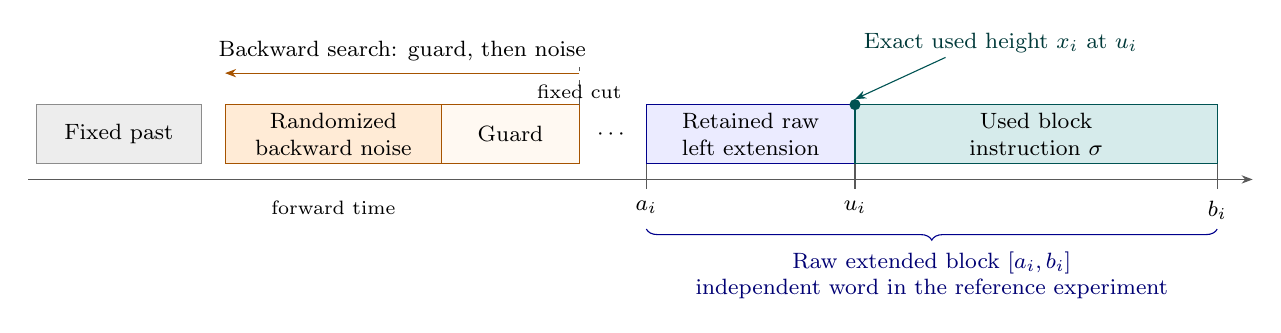
\begin{tikzpicture}[x=1cm,y=1cm,font=\footnotesize,
  resample label/.style={align=center,inner sep=2pt},
  resample tick/.style={draw=black!65,line width=.5pt}]
  \filldraw[fill=black!7,draw=black!45] (0,.2) rectangle (2.1,.95);
  \filldraw[fill=orange!16,draw=orange!65!black]
    (2.4,.2) rectangle (5.15,.95);
  \filldraw[fill=orange!5,draw=orange!65!black]
    (5.15,.2) rectangle (6.9,.95);
  \filldraw[fill=blue!8,draw=blue!55!black]
    (7.75,.2) rectangle (10.4,.95);
  \filldraw[fill=teal!16,draw=teal!65!black]
    (10.4,.2) rectangle (15,.95);

  \node[resample label] at (1.05,.575) {Fixed past};
  \node[resample label] at (3.775,.575) {Randomized\\backward noise};
  \node[resample label] at (6.025,.575) {Guard};
  \node[resample label] at (7.325,.575) {$\cdots$};
  \node[resample label] at (9.075,.575) {Retained raw\\left extension};
  \node[resample label] at (12.7,.575) {Used block\\instruction $\sigma$};

  \draw[-{Stealth[length=4pt]},black!65] (-.1,0) -- (15.45,0);
  \node[anchor=north,font=\scriptsize] at (3.775,-.15) {forward time};
  \foreach \t/\name in {7.75/a_i,10.4/u_i,15/b_i} {
    \draw[resample tick] (\t,.2) -- (\t,-.12);
    \node[anchor=north] at (\t,-.15) {$\name$};
  }

  \draw[resample tick,dashed] (6.9,.95) -- (6.9,1.43);
  \draw[-{Stealth[length=4pt]},orange!65!black]
    (6.9,1.35) -- (2.4,1.35);
  \node[resample label,anchor=south] at (4.65,1.43)
    {Backward search: guard, then noise};
  \node[resample label,anchor=north,font=\scriptsize]
    at (6.9,1.28) {fixed cut};

  \fill[teal!65!black] (10.4,.95) circle (2pt);
  \draw[-{Stealth[length=4pt]},teal!65!black]
    (11.55,1.55) -- (10.4,1.02);
  \node[resample label,anchor=south,text=teal!45!black]
    at (12.25,1.53) {Exact used height $x_i$ at $u_i$};

  \draw[decorate,decoration={brace,mirror,amplitude=4pt},blue!55!black]
    (7.75,-.63) -- (15,-.63);
  \node[resample label,anchor=north,text=blue!45!black]
    at (11.375,-.84) {Raw extended block $[a_i,b_i]$\\
      independent word in the reference experiment};
\end{tikzpicture}
\caption{One block in the local resampling decomposition; ordinary pieces
are suppressed.  The exact height $x_i$ is retained at the used start
$u_i$.  The local observation uses the raw word on $[a_i,b_i]$, this
height, and the used-portion instruction $\sigma$.  Noise paths and
randomized depths are nuisance resampling data; guard words and cut times
are fixed.  Extension-only external $F$'s receive deterministic surrogate
types for recording the contour, without changing the local observation.}
\label{fig:local-resampling}
\end{figure}


Let $x_i\in\mathbb Z^2$ be the actual height at the used start $u_i$
of retained block $i$.
After freezing the outside initial height, the guards, cut positions,
and the instructions, the successive noise displacements are
\begin{equation}\label{loc:triangular-map}
 d_1=x_1-c_1,\qquad
 d_i=x_i-x_{i-1}-c_i\ (2\le i\le r),\qquad
 d_{r+1}=h_*-x_r-c_{r+1}.
\end{equation}
The last term is present only when the terminal height $h_*$ is fixed.
For clarity, let $A_i$ be the actual imposed increment from the end of
noise $i$, through its guard and ordinary pieces and the current raw
extension, to $u_i$.  Let $B_{i-1}$ be the actual imposed increment from
$u_{i-1}$ to the start of noise $i$.  Then
$c_i=B_{i-1}+A_i$, with the corresponding initial and terminal versions.
These increments use the stable \emph{global} instructions and the
fixed guard context.  They are exact functions of the raw pieces,
including the current retained prefix, independent of the free noise
displacements.  They are not equated with the deterministic surrogate
increments used to record extension paths.  Their normalized difference
from the corresponding surrogate increments is bounded by the
unidentified-$F$ counts of finitely many independent raw blocks and
vanishes in reference probability.  The first
$r$ equations are a triangular integer affine bijection with determinant
one.  At even retained cuts, $x_i^{(1)}+x_i^{(2)}$ is even up to the
fixed origin convention.  The parity of the last equation is then
automatic from the elapsed times and the fixed endpoint.  Projecting the
$x_i$ to a forest introduces precisely the fixed fiber factors of
Lemma~\ref{loc:projection-density}.

For a fixed decomposition, let $q_{j,N}(t,d)$ be the iid probability of
noise $j$ having duration $t$ and displacement $d$, including its
independent randomized-depth probability.  The conditional law of its
raw path given those parameters is denoted by $\mathcal B_{j,N}^{t,d}$.
If the full heights are sampled in the reference experiment with mass
$r_N(x)$, the unfrozen words and full heights have, before normalization,
density
\begin{equation}\label{loc:exact-density}
 \frac{\prod_j q_{j,N}(t_j,d_j(x))}{r_N(x)}
 \;\mathbf 1_{\mathcal T_N}
\end{equation}
relative to independent raw ordinary and retained blocks and the
reference heights.  Conditional noise paths are sampled independently
from $\mathcal B_{j,N}^{t_j,d_j(x)}$.  Here $\mathcal T_N$ is the
chosen stable contour/parameter cell, including strict containment of
the decomposition.  Factors depending only on frozen observations have
been omitted, since they cancel in the conditional ratio.

The finite experiment also freezes a suffix's resolved types. Equal
entrance heights alone need not preserve its flexible decisions: those
decisions compare burger identities. The next two statements supply the
required protection near the terminal endpoint.

\begin{lemma}[Protected prefix ranks]\label{loc:protected-prefix-stacks}
Run two replacement words from the same fixed prefix.  Suppose the
type-$i$ stack size never falls below an integer $m_i$ during either
replacement, and their two ending stack sizes agree.  At their end the
occupied ranks at most $m_i$ agree by burger identity, for each type.
Now process a common frozen suffix with prescribed flexible types.
Until a first incorrect prescribed decision, all occupied ranks at most
$m_i$ continue to agree.  In particular, a prescribed $F$ decision
correct in one run is correct in both whenever both current type-stack
sizes are at most their respective $m_i$.
\end{lemma}
\begin{proof}
Removing an original burger of rank at most $m_i$ during a replacement
would lower that stack size below $m_i$, which is excluded.  During the
suffix, equal prescribed types give equal heights.  Removing above rank
$m_i$ does not change a protected rank; removing at such a rank removes
the same identity in both runs.  A frozen suffix addition at such a rank
also has the same identity in both runs.  Induction proves agreement of
all occupied protected ranks, even after the suffix dips below its
original floor.  At the specified $F$ step the two available top burgers,
or their absence, therefore agree exactly.  Their creation-time
comparison agrees as well.
\end{proof}

\begin{corollary}[Automatic terminal flexible decisions]
\label{loc:terminal-flexible-orders}
Fix an enclosing mutable interval strictly inside a positive quadrant
excursion and freeze the exterior prefix and suffix.  There are positive
constants $c_1,c_2$ and a terminal collar such that, in a sufficiently
small contour tube, all mutable paths stay above
$m_i=\lfloor c_i\sqrt N\rfloor$, and all provisionally resolved suffix
heights in that collar are at most $m_i$.  If the mutable interval ends
at the fixed suffix entrance heights and the imposed suffix decisions
are correct before the collar, every decision in the collar is correct.
Consequently the resampled word is empty precisely when its imposed
heights stay nonnegative and end at zero.
\end{corollary}
\begin{proof}
Choose each $c_i$ below half the minimum of the limiting coordinate on
the mutable interval.  Its positive minimum exists by strict interior
excursion positivity.  The excursion coordinates tend to zero at the
terminal endpoint, so choose a collar with both coordinates below
$c_i/2$.  Uniform convergence, with sufficiently small tube radius,
gives the asserted integer inequalities.  The provisional suffix has
the same heights in both runs because its entrance heights and its
resolved increments are fixed.  Apply
Lemma~\ref{loc:protected-prefix-stacks} at a first allegedly incorrect
terminal decision.  Nonnegative actual heights exclude unfilled orders,
and zero final heights leave no burgers.
\end{proof}

\begin{remark}
Equal endpoint heights and a guard alone would not prove this
corollary.  With prefix $hc$, replacing a subsequent $hc$ by $ch$ leaves
the same endpoint heights but can change the next flexible choice after
a fixed $hH$ guard.  Protected low ranks, or the separated supplier
comparisons before the collar, are necessary.
\end{remark}

\begin{lemma}[Validity of the finite density identity]\label{loc:resampling-identity}
Equation~\eqref{loc:exact-density} is an exact identity for the iid
experiment on a fixed decomposition and stable cell.  In the
empty-word experiment it is also exact after fixing the exterior prefix,
the exterior suffix and its resolved types, and the resulting exact
terminal height, provided the terminal consistency condition in
Corollary~\ref{loc:terminal-flexible-orders} is imposed.  The
identity involves no local-limit assertion for the probability of an
empty word.
\end{lemma}
\begin{proof}
Expand the conditional probability as a finite sum over raw words and
auxiliary depth choices.  The iid letter weight factors over the
disjoint pieces.  Being a guard or a noise is a property of its own
word: its successive retained type-1 burgers are detected by backwards
inspection, and every $F$ there resolves internally.  Thus summing over
noise words with a specified duration and displacement gives exactly
$q_{j,N}$, and conditioning on those parameters gives
$\mathcal B_{j,N}$.  The guard and exterior-prefix probabilities are
constant in the ratio.  All interior ordinary pieces retain their
independent raw letter weights.  Lemma~\ref{loc:first-error}
makes the imposed ordinary resolutions genuine for every word in the
stable cell.  Changing variables by
Equation~\eqref{loc:triangular-map} and dividing by the reference mass
$r_N$ proves the iid identity.

For the conditioned experiment, initially retain both indicators: the
concatenated word reduces to the empty word, and its suffix has the
prescribed resolved types.  The empty-word normalizing constant and the
raw exterior weights cancel on the frozen atom.  The exact entrance
height of the suffix is determined by its prescribed net increment and
the terminal value zero.  It is the $h_*$ in
Equation~\eqref{loc:triangular-map}.  Positivity and the stable
instructions make the two retained indicators equal to one before the
terminal collar; Corollary~\ref{loc:terminal-flexible-orders} makes them
equal to one there as well.  The remaining ratio is exactly
Equation~\eqref{loc:exact-density}.
\end{proof}

The exact identity is now established. To identify a limiting kernel, we
must show that its density loses all dependence on microscopic information
beyond the retained observation's macroscopic input.

\begin{proposition}[Macroscopic form of the resampling density]
\label{loc:macroscopic-density}
Fix a finite stable decomposition and restrict its macroscopic
parameters to a compact set on which all noise durations are positive,
all randomized first displacements are strictly inside their support,
and the reference height density is positive.  Include among the
macroscopic nuisance variables the frozen contour pieces, integrated
ordinary pieces, and the conditional noise contours.  Fix a subsequential
limiting law of the actual frozen data.  The continuity cells can be
chosen so that, for almost every frozen value under this law and every
sequence of frozen data converging to that value, the density in
Equation~\eqref{loc:exact-density}, after multiplication by its common
power of $N$ and fixed lattice factor, converges in the form required by
Lemma~\ref{loc:weighted-transfer}.  Its limit depends only on the
macroscopic variables.  On every cell containing a compatible strict
path tube, its limiting normalizing integral is positive.  Here finite
frozen data range over atoms having positive probability in the chosen
stable cell.  In particular, a suffix-type atom comes with an actual
compatible word in that cell for the protected-rank comparison.
\end{proposition}
\begin{proof}
First keep all noise durations fixed and use full height parameters.
Each noise mass is $N^{-2}$ times a positive continuous function, up to
a uniform $o(N^{-2})$, by Corollary~\ref{loc:noise-density}.  The
reference mass for $r$ two-dimensional heights is $N^{-r}$ times its
positive continuous density and its fixed lattice cell volume.  With a
terminal noise the quotient in
Equation~\eqref{loc:exact-density} therefore has common factor
$N^{-r-2}$.  Without that noise the corresponding factor is $N^{-r}$.
These factors cancel in the normalized conditional law.  The remaining
quotient converges uniformly on the compact parameter set to the product
of the translated functions in Equation~\eqref{loc:hitting-density}
divided by the reference height density.

The translations in Equation~\eqref{loc:triangular-map} are exact
functions of the raw words, guard context and global instructions.
Their normalized limits depend only on the recorded increment paths.
In particular the true extension increments in $A_i$ need not equal
the locally recorded surrogate increments: their difference is bounded
by twice the corresponding raw unidentified-$F$ counts.
Unresolved flexible counts in independent raw blocks are
$o_{\mathbb P}(\sqrt N)$, so the macroscopic block limits are the
ordinary Brownian increment laws, for every one of the finitely many
instructions.  The extra global extension instructions do not enter
the local observation: its exact heights are anchored at $u_i$ and it
uses only the local used-portion instruction.  Changing those extra
instructions changes neither $Y_N$ nor the reference limiting input,
and hence does not change the extracted joint law or its kernel.
Every interior ordinary gap is likewise a free raw nuisance block.
Its actual resolution under the global guard context may depend on
neighboring retained words, but its difference from any fixed local
surrogate is bounded by twice its own unidentified-$F$ count.  The same
unconditioned estimate therefore gives its macroscopic increment path.
Only the exterior prefix and the finite suffix with prescribed types
enter through fixed resolved paths; guards resolve internally.  No
conditional unidentified-letter estimate for frozen interior words is
used.

Conditional noise contours converge by
Lemma~\ref{loc:ladder-llt}, uniformly on the compact endpoint set.
Their exact endpoints may depend on additional raw extension data and
global instructions beyond $C_N$.  Those normalized endpoints differ by
$o_{\mathbb P}(1)$ from the endpoints computed from $C_N$ and the
macroscopic ordinary nuisance paths.  Uniform bridge-kernel convergence
and continuity therefore replace the former by the latter in $L^1$
for bounded continuous conditional tests.  This proves the limiting
factorization with $K_c$; finite-$N$ conditional independence given
$C_N$ alone is not required.
They can therefore be adjoined as continuous conditional nuisance
kernels in Lemma~\ref{loc:weighted-transfer}.  Concatenation of finitely
many continuous paths with positive durations and the prescribed endpoint
translations is continuous.  For each of the countably many tube centers
and decomposition patterns, mix the limiting reference resampling law
over the actual limiting frozen-data law.  A real-valued tube-distance
variable has only countably many atoms under this mixture.  Choose a
countable dense family of radii avoiding the union of these atom sets.
Fubini's theorem then gives a full-measure set of frozen values on which
all the chosen boundaries have zero conditional reference mass.
Multiplication by the bounded limiting density preserves that assertion.
For a sequence of frozen data converging to a value in this set,
conditional bridge convergence and continuity of concatenation imply
that the cell indicators converge in $L^1$ in an almost sure coupling.
Together with the uniform density approximation this is the required
$L^1$ macroscopic tilt approximation.  This argument asserts a common
full-measure set for the actual mixture; it does not assert conditional
boundary continuity at every possible frozen contour.

If only forest parameters are retained, complete them by auxiliary full
heights with a positive smooth density and integrate along fibers.
Lemma~\ref{loc:projection-density} proves the same assertion with the
correct projected lattice factor.  If durations are integrated, sum the
local-limit masses against the original smooth cut density.  Its
Riemann-sum factors appear identically in numerator and denominator.
One must not freeze a randomized first-depth count in this calculation:
that would remove one of the free displacement coordinates.

For positivity, take a compatible parameter/path tuple in the interior
of the cell.  Shrink to a product of path tubes and a small parameter
neighborhood still in the cell.  The endpoint densities and reference
height density have positive lower bounds there.  Free Brownian blocks
have positive probability to follow each required tube, and the
conditional noise bridges do too by
Lemma~\ref{loc:ladder-llt}.  Thus the limiting weighted integral over
this smaller set is positive.  This argument is stable in a neighborhood
of the frozen macroscopic data.  Its lower bound may depend on that data
and the chosen cell; no uniform lower bound as cells shrink is asserted.
\end{proof}

\subsection{Common kernels and changes of scale}

The local limit turns the exact density into a macroscopic tilt on each
stable cell. Exhausting those cells identifies the kernel conditional on
the complete contour. We then repeat the discrete approximation argument
to allow further limits and changes of quantum units.

\begin{theorem}[Common conditional kernels on fixed charts]
\label{loc:fixed-chart-kernels}\label{loc:finite-transfer}
Fix a finite collection of protected time charts, fixed instructions,
and measurable $E$-valued observations of their raw words and exact
parameters.  Extract their independent reference experiments jointly as
in Equation~\eqref{loc:reference-law}.  Consider either the bilateral
inventory word or a finite word conditioned to be empty.  In the finite
case keep every chart in a strict interior time interval.  Use the same
time and distance units in the reference and actual experiments.

In every joint subsequential limit, conditional on the complete limiting
contours, the retained cuts and marks locating the charts, and any
independently adjoined surface-coordinate data, the
observations have the reference kernels evaluated at their chart inputs.
For charts in disjoint spatial buffers these kernels are conditionally
independent.  The assertion includes the universal endpoint
observations, not only existential path certificates.
\end{theorem}
\begin{proof}
It suffices initially to test finitely many bounded continuous functions
of the observations and of the contour on a bounded time window.
Choose deterministic enclosing slots inside the positive gaps between
the extended blocks.  In each slot use a noise and guard as above.  A
countable choice of enclosing slots suffices because the gap conditions
are strict.  If the block cuts are Poisson cuts, retain their smooth
joint density inside these enclosing slots rather than conditioning on
each of their microscopic durations.  Noise and guard endpoints may be
conditioned on separately; they are determined in the reserved slots.

The noise and guard pieces fit with probability tending to one as
$a\downarrow0$, after $N\to\infty$.  Indeed their total backwards
depth is at most $3a\sqrt N+O(1)$.  The contour invariance principle
identifies their duration with a backwards Brownian first passage to a
level tending to zero at an ordinary interior time.  That duration tends
to zero in probability.  This applies under the finite excursion law
by its interior absolute continuity.  With $a$ fixed, guards and noises
have positive limiting durations.  These durations, supplier windows,
depths, and displacements can be truncated to compact interior sets
with arbitrarily high actual probability.

On this truncated event, Brownian genericity and
Lemma~\ref{loc:finite-instructions} give finitely many stable signs on
a sufficiently small contour tube.  Before the first reserved slot use
the actual unchanged past.  Between slots apply
Lemma~\ref{loc:first-error} successively.  In the finite experiment,
freeze the raw exterior prefix and suffix, the suffix's resolved types,
guard words and endpoint cuts.  The height at the end of the mutable
region is then the negative of the prescribed suffix increment.
Keep the randomized noise depths free.  The protected-rank
Corollary~\ref{loc:terminal-flexible-orders} handles the final collar;
the separated comparison instructions handle the remaining suffix.

Disintegrate after restricting to the actual stable cell.  Every frozen
atom under consideration then has positive probability in that cell and
supplies an original correctly resolved word satisfying its protected
floors.  The exact conditional distribution on each such atom is
Lemma~\ref{loc:resampling-identity}.  Along convergent frozen
data, Proposition~\ref{loc:macroscopic-density} gives a macroscopic
density with positive limiting denominator.  The actual limiting paths
are in the required support: the free blocks are Brownian paths under
interior excursion absolute continuity, and the selected noises are
first-passage portions with positive duration and interior randomized
depth.  An open tube about such a tuple contains a smaller compatible
product tube of the type used in the positivity proof.

Apply Lemma~\ref{loc:weighted-transfer}.  The full limiting contour on
the window is reconstructed by concatenating the retained block paths,
noise paths, integrated interior ordinary paths, and the fixed resolved
exterior paths, with the displayed
height translations and exterior absolute time origins.  The retained
cut and mark data locate each chart in that contour, so the pair
determines its intrinsic input $C$.  Conditioning on this pair therefore
leaves the reference observation kernel unchanged.  For deterministic
cuts the extra cut data are redundant; for random cuts they are part of
the conditioning sigma-field.  In the bilateral experiment
there is no terminal empty-word factor.  Any further exterior contour
window may be included among the nuisance pieces; unidentified flexible
effects there are negligible in rescaled increments.  In the finite
experiment the prescribed exterior increments are exact after the
terminal consistency argument.

After extracting the actual limiting frozen-data law, choose continuity
cells as in Proposition~\ref{loc:macroscopic-density}.  Intersect its
full-measure admissible set with the generic, strict-margin set.  The
preceding assertions hold along every sequence of frozen data converging
to a value in this intersection.  Couple the actual frozen data, apply
this sequential assertion almost surely, and integrate as in
Lemma~\ref{loc:weighted-transfer}.  Exhaust the
compact parameter cutoffs, the supplier windows and the countable
stable cells.  Their omitted actual probabilities tend to zero.  A
monotone-class argument for continuous cylinder tests and increasing
time windows gives conditioning on the complete contour.

For disjoint buffers, Lemma~\ref{bg:protected-atlas} uses disjoint
raw block families.  Sample their shift parameters independently in the
product reference experiment.  The union of their coordinate forests is
again an admissible forest; the calculation above permits the actual
macroscopic height constraints to couple those parameters but not their
conditional observation kernels.  Hence the reference product kernels
remain products after conditioning on the complete contour.  All
arguments applied to arbitrary $E$-valued measurable functions of the
finite chart, so they also apply to the universal endpoint variables.
\end{proof}

\begin{proposition}[Closure under varying laws and changes of units]
\label{loc:kernel-closure}
Fix the model parameter $q$.  Form the joint array consisting of all marked certificate and universal
observations under consideration, their contours and cut data, and the
independent reference experiments for a countable list of fixed charts,
refinements, instructions and quantum offsets.  Use one common Polish
array schema, with matching actual and reference readouts in every row.
Retain the full canonical
joint continuum input: contours, cuts and marks, decorated surface
fields, and reference internal metrics on countably many fixed collars.
Fix its law in the chosen units; in the bilateral applications this is
the scale-covariant continuum law.  Its charts have the positive
durations, extension lengths, gaps and Brownian-generic inputs required by
Theorem~\ref{loc:fixed-chart-kernels}.  For finite experiments require
also the strict interior endpoint margins of that theorem.
Call a law admissible if it is a joint
subsequential law of these arrays from the discrete inventory experiments,
with this continuum marginal, arbitrary deterministic positive cost
units, and every fixed retained time unit tending to infinity in lattice
units.  The continuum coordinates belong to this same joint approximating
coupling and satisfy the conditional-independent augmentation convention
at the start of this section; a fixed continuum marginal alone is not
the definition of admissibility.

The admissible family is closed under further weak extraction, including
extraction from a varying sequence of admissible laws.  The same holds
after deterministic changes of the base quantum units and relabeling the
fixed offsets, provided the corresponding discrete arrays are retained
and the target continuum marginal has these same genericity and strictness
properties.  Actual and reference coordinates use identical target time
and cost units, and each chart keeps its positive durations, extensions
and gaps in its own normalized coordinates.  Each reference coordinate has smooth duration and shift
densities in its own normalized units; it is not obtained by allowing one
old density to degenerate under the changing zoom.
Every resulting law has the fixed-chart common-kernel identities of
Theorem~\ref{loc:fixed-chart-kernels}; its independent disjoint-chart
reference experiments give product conditional kernels.  Consequently
the spatial, restriction and field-density conclusions below hold anew
in that law.  Kernels may change with the law: the assertion identifies
them with the reference kernels extracted in the new joint array.
The fixed full joint continuum marginal remains the same in the further
limit.
\end{proposition}
\begin{proof}
Use a metric $d_{\rm w}$ for weak convergence on the countable product
of the observation spaces and their Polish contour and auxiliary spaces.
Let $\mathcal L_j$ be
admissible laws converging to $\mathcal L$.  By admissibility, for row
$j$ choose a discrete approximant whose law is within $1/j$ of
$\mathcal L_j$ in $d_{\rm w}$.  Choose it
far enough along its defining sequence that each of the first $j$
retained time units exceeds $j$ lattice steps and all the prescribed
finite coordinate approximations hold.  The triangle inequality gives
a single diagonal array converging to $\mathcal L$.

If a continuum coordinate has no discrete definition, retain its actual
joint coupling as follows.  Couple a row's discrete raw arrays to their
limit almost surely, adjoin the row's canonical continuum tuple with
its prescribed law conditional on the complete limiting contour and
cut data, independently of the entire coupled actual and reference
observation array, and attach the same tuple along the row.  This gives
joint convergence and preserves
every discrete raw-word marginal.  The resampling identity is applied
to those raw coordinates; the canonical contour-to-surface and
field-to-metric relations are used only in the limiting continuum
readout.

Each diagonal row is still an actual raw-word experiment with its
independent reference experiments.  Equation~\eqref{loc:exact-density}
is valid there before any limit.  Apply its local-limit and macroscopic
transfer proof to this diagonal sequence, choosing continuity cells for
its actual limiting frozen-data mixture.  The retained canonical joint
marginal supplies genericity, positive durations and gaps, and the
required finite-volume endpoint margins in the limiting chart.  Thus
the free raw letters,
positive-duration compact truncations and cost compactification are the
same as in Theorem~\ref{loc:fixed-chart-kernels}.  The time unit is
allowed to vary with the row, and the proof imposes no restriction on
the deterministic cost denominator.  Thus the theorem produces the
new conditional kernels.  Products of independent reference laws
remain products under joint weak convergence; their disintegrations
give the asserted factorization.  Countable selection and the same
local field-density argument then give the spatial conclusions.

For a change of base units, first apply that fixed change in row $j$,
including it in every retained actual and reference coordinate, and only then
choose its sufficiently fine discrete approximant.  This ensures the
required divergence of every fixed rescaled lattice time unit even
when the base change varies with $j$.  Include the countable union of
the row-wise relabeled coordinates, and sample each target reference
density directly in its normalized units.  Projection onto the retained
continuum coordinates proves the last assertion.  In particular no
continuity of the map from a field to its internal metric is needed:
the entire contour/mark/field/metric coupling is retained.
For a random auxiliary continuum coordinate $A$ beyond the complete
contour and cut data $\mathcal C$, the extension of conditioning follows
from its fixed joint law with $\mathcal C$.  Given a bounded continuous
test $\phi(A)$, approximate $\mathbb E[\phi(A)\mid\mathcal C]$ in
$L^1$ of the fixed $\mathcal C$ marginal by bounded continuous functions
of $\mathcal C$.  The row-wise conditional identity, tested against
bounded continuous functions of $(\mathcal C,Y)$, then passes to
the limit with an error uniform in the row.  Letting the $L^1$ error
vanish preserves conditional independence of $A$ and the observations
given $\mathcal C$.  Deterministically reconstructed continuum coordinates are
the immediate special case.
This proof uses discrete approximation and the exact density again;
it does not assert weak closure of abstract conditional-independence
relations or pointwise convergence of regular conditional kernels.
\end{proof}

\subsection{Spatial selection and changes of field law}

We have proved the kernel identities for fixed chart descriptions. A
spatial observation chooses its chart using local continuum geometry.
The following conditional-expectation identity permits that choice once
the evaluated selected kernel is measurable in the stated local data.

\begin{lemma}[Countable selection of conditional kernels]
\label{loc:countable-selection}
Let $\mathcal C$ be a standard Borel macroscopic variable and let
$Y_j$, $j\in\mathbb N$, be a countable consistent family of observations.
Suppose, for each $j$, its conditional law given $\mathcal C$ is
$K_j(T_j(\mathcal C),\cdot)$.  Let $J$ be measurable with respect to
$\sigma(\mathcal C)$, and suppose the selected probability kernel
\[
                       Q=K_J(T_J(\mathcal C),\cdot)
\]
is measurable with respect to a smaller macroscopic sigma-field
$\mathcal H\subset\sigma(\mathcal C)$.  Then, for every bounded
measurable $f$,
\[
 \mathbb E[f(Y_J)\mid\mathcal C]=Qf,
 \qquad
 \mathbb E[f(Y_J)\mid\mathcal H]=Qf.
\]
In particular, this applies if both $J$ and $T_J$ are
$\mathcal H$-measurable.
The same assertion holds for finite selections with product joint
conditional kernels.  Countable exhaustions of consistent observations
inherit the resulting kernel.
\end{lemma}
\begin{proof}
Multiply the conditional identity for $Y_j$ by
$\mathbf 1_{\{J=j\}}$ and sum over $j$.  This proves the first identity.
The assumed measurability of $Q$ and the tower property give the second.
Products of test functions prove the finite joint assertion, and a
monotone-class argument using cylinder functions proves the exhaustion
assertion.
\end{proof}

Let $h^{\rm IG}$ denote the imaginary field modulo its period.  Area
marks can be realized as a Poisson process on
$\mathbb C\times(0,\infty)$ with conditional intensity
$\mu_h(dz)\,du$; marks of level at most a prescribed intensity give the
nested time-cut experiments.  Restrictions to disjoint spatial sets are
conditionally independent given $h$.

\begin{theorem}[Local spatial kernels with separate field buffers]
\label{loc:spatial-kernels}
Let $K\Subset U$ be a compact confinement in an open real-field domain,
and let $V$ be an open imaginary-field domain containing a neighborhood
of $\overline U$.  One may alternatively first replace $U$ by any
relatively compact neighborhood of $K$ inside it.  The limiting local
certificate and universal-endpoint observations in $K$, interpreted with
open loss inside $U$, have conditional kernels measurable in
\begin{equation}\label{loc:local-sigma-field}
 h|_U,\qquad h^{\rm IG}|_V\pmod{\text{period}},\qquad
 \text{area marks in }U,\qquad O,
\end{equation}
where $O$ is the finite relative global order of the buffered local
traversals needed by the observation.  Conditional on the complete
continuum fields, curve, and marks, observations in disjoint real-field
buffers have independent kernels.  The imaginary buffers may be larger
and may overlap for this conditional-independence assertion.

The kernels are intrinsic under changes of the quantum-surface
coordinate representation.  They are the same in the bilateral and
strict-interior finite-excursion experiments with common time and distance
units.  No fixed positive separation between the test and the real-field
boundary is required uniformly across all applications: any prescribed
$K\Subset U$ is allowed before taking the limit.
\end{theorem}
\begin{proof}
Choose nested neighborhoods
\[
 K\subset\operatorname{int}K_*\Subset U_0\Subset U_1\Subset U.
\]
The imaginary field on $V$ reconstructs all directed $U_1$-traversals
reaching $\overline U_0$.  There are finitely many such traversals,
as in Lemma~\ref{bg:protected-atlas}.  The real field on $U$ gives
their quantum-area clocks and the quantum lengths of their labelled
frontier arcs.  Retain their genuine relative order $O$.  This order
compares visits in distinct traversals; the directed clocks compare
visits in the same traversal.  No absolute origin on the global tour
is required for these comparisons.

We describe the local tests used to select a protected chart.  At a
fixed Poisson refinement, choose finitely many used blocks inside these
clocked traversals, with their closures in $U_0$, and left extensions
with closures in $U_1$.  Require their used interiors to cover every
visit to $K_*$.  This is a test on the reconstructed finite traversal
family: every visit to $K_*$ lies in one of its members.  The marks in
$U$ locate the cuts along each directed clock.  They therefore give the
block durations and extension offsets, even though they do not give the
absolute global Poisson indices of those cuts.  The local frontier
lengths give the two increment paths, pinned at each used start.

For these blocks, Lemma~\ref{bg:local-ports} gives the two labelled
port relations and the forest differences within each overlap
component.  Evaluate the retained suffix, prefix and intervening
minimum tests using these paths and differences.  Among the protected
candidates passing those tests, the port relation distinguishes the
genuine contacts from the other candidates.  Select the rational band
which strictly separates their height sets, with the empty-set
conventions in Lemma~\ref{bg:omitted-clearance}.  Its existence follows
from that lemma.  Its selection uses the two local height sets, not the
value of a minimum in an omitted gap.

The flexible-order instruction is selected from the same data.  Consider
the possible pairs of scalar suppliers for a decision in a used block,
with each supplier at or before that block's left-extension start.  Their scalar
contacts are read from the labelled frontier relations.  Each supplier
has the same spatial image as the decision, so its visit occurs in the
retained family of $U_1$-traversals.  The closed scalar contact relations
on the finitely many closed traversal records make the candidate set
compact.  Positive extension duration separates its suppliers from
the used decision times.  The order $O$ and the directed clocks decide
which member of the pair is later.  The two possible orders therefore
give compact disjoint sets of decision times, by the argument of
Lemma~\ref{loc:finite-instructions}.  Choose a finite rational partition
of the used clock whose boundaries avoid these sets, and prescribe the
corresponding type on each part.  This is the local test for an
admissible instruction.  A bounded global supplier window and a small
tube for the complete contour are used in
Lemma~\ref{loc:first-error} to prove that the selected instruction is
eventually correct in the discrete words.  They are not inputs to its
local selection.  The same distinction applies to the omitted minima
used to prove band clearance.

Thus the data in Equation~\eqref{loc:local-sigma-field} determine a
finite intrinsic description: the retained block pattern, side labels,
forests, rational bands and flexible instructions.  They also determine
its continuous input: intrinsic durations and extension offsets,
used-start-pinned increment paths, and the forest differences.  All
choices are taken from the countable atlas and may be made by its fixed
enumeration.  Extension-only external $F$'s keep their deterministic
surrogate types.  Their normalized typing error vanishes under the
independent reference law by Proposition~\ref{arm:uniform-past-limit};
their exact types do not enter
the local observation because its heights are anchored at used starts.
The extra global instructions used to prove the resampling identity
likewise contribute no additional input to this observation.

To apply countable selection, distinguish this intrinsic description
from the global labels locating its blocks in the complete contour.
Those labels are measurable from the complete contour and cut data.
They need not be measurable from the local fields.  The reference
experiment, however, samples only the intrinsic raw blocks, durations
and shifts; its observation uses no absolute tour start or omitted-gap
duration.  Two realizations of the same intrinsic description therefore
use the same reference experiment and observation after relabelling
their blocks.  Smooth changes of the reference duration or shift
densities leave its conditional kernel unchanged by
Lemma~\ref{loc:weighted-transfer}.  For the countable atlas, choose
these common kernel versions simultaneously.  Consequently the
reference kernel evaluated at the selected chart depends only on the
local intrinsic description and input just constructed.

Theorem~\ref{loc:fixed-chart-kernels} supplies the conditional identity
for every globally located member of the atlas.
Lemma~\ref{loc:countable-selection} now applies because its selected
evaluated kernel is local.  Exhaust the finite observations and rational
open losses to obtain the asserted spatial kernel.  This selection is
performed on the limiting continuum data, after the fixed-chart
identities have been proved.  Because the chart observations were
extracted jointly, restriction from a larger protected chart to a smaller
one is a measurable projection of that same family, so the kernels
inherit restriction compatibility.  Versions may be fixed for the
countable atlas and the countable deterministic field changes used
later, since absolute continuity preserves their common null sets.

For disjoint $U$ the protected retained block families are disjoint.
The reference experiment and Theorem~\ref{loc:fixed-chart-kernels}
therefore give product kernels conditional on the complete continuum
data.  Selection of their indices by that data preserves the product
identity.  Overlap of the imaginary buffers is harmless here, because
the entire imaginary field is conditioned on.  To use independent
Dirichlet field parts in a later resampling experiment one separately
chooses disjoint imaginary testing domains.

The complete cone or sphere contour supplies its ambient decorated
surface by Theorem~\ref{bg:continuum-inputs}(ii).  Apply the local atlas
directly to that surface's fields and traversals.  Write $\ell$ for
the data in Equation~\eqref{loc:local-sigma-field}, $s(\ell)$ for
the selected intrinsic description, and $c(\ell)$ for its intrinsic
input.  The same data give a map $\Phi_{s(\ell)}^\ell$ from its
intrinsic time records to spatial records along the local traversals.
The spatial conditional kernel is consequently
\[
 Q_\ell
   =\bigl(\Phi_{s(\ell)}^\ell\bigr)_*
       K^{s(\ell)}_{c(\ell)}.
\]
All three constructions use the same local data in the cone and sphere
settings, and Theorem~\ref{loc:fixed-chart-kernels} supplies the common
reference kernel $K^s_c$ in both.  The clocks, quantum frontier lengths,
used-start height differences and side labels are intrinsic under
conformal coordinate changes.  Transporting the local fields and
traversals therefore transports the spatial record while preserving
its intrinsic conditional law.  This proves covariance and the common
cone/sphere interpretation with the actual field normalization retained.
\end{proof}

\begin{corollary}[Field-density transfer and local pasting]
\label{loc:field-tilt}
The spatial kernels in Theorem~\ref{loc:spatial-kernels} are unchanged
under a locally absolutely continuous change of the continuum field law.
For a Cameron--Martin modification, work with an actual Gaussian local
reference field and a fixed compactly supported smooth real function $f$
in its Cameron--Martin space. In the circle-average-pinned whole-plane
reference used below, it suffices to choose the pinning circle outside
$\operatorname{supp}f$.

One may then use the kernel for $h+f$ on a compact interior patch and
retain the kernel for $h$ outside a larger disjoint neighborhood on which
$f=0$. Conditional on the fields these are the prescribed product
kernels. The resulting subprobability comparison is made before selecting
a hit or a shortcut event. This is a comparison in the Gaussian reference
law; it does not assert that an arbitrary shift preserves the global
unit-area normalization of a sphere.
\end{corollary}
\begin{proof}
If a joint law has disintegration $\mu(dc)K_c(dy)$ and the field law is
tilted by a density $R(c)$, its joint law is
$R(c)\mu(dc)K_c(dy)$.  Thus the conditional kernel is unchanged as a
function of the realized macroscopic input.  Bounded density
approximations and truncation give the assertion for an arbitrary
absolutely continuous tilt.  The fields and any embedding gauge may be
included in the macroscopic data: the gauge is adjoined conditionally
independently of the microscopic observations given the contours.

For $f$ in the specified Cameron--Martin space, the Cameron--Martin
theorem gives the field density with the actual normalization retained.
A shift with nonzero average on a fixed pinning circle would move the
field to a disjoint affine support, so that case is not covered.  Apply
Theorem~\ref{loc:spatial-kernels} to the shifted interior and unchanged
exterior patches.  Resample the area marks inside the changed region
with their correct conditional intensity $\mu_{h+f}$ and retain the
marks outside, where the intensity is unchanged.  All chart refinements
can be coupled this way.  Conditional product kernels then give the
stated joint law on the two separated regions; extend to the unobserved
region by a regular conditional distribution.  Only afterward restrict
to a selected input event and bound the Cameron--Martin likelihood.
In particular, a larger imaginary buffer in
Theorem~\ref{loc:spatial-kernels} does not enlarge the support required
for this real-field modification.
\end{proof}

\begin{remark}
Corollary~\ref{loc:field-tilt} is a statement about conditional laws.
It does not identify a passage realization at $h+f$ with a deterministic
length reweighting of one at $h$.  Weyl scaling will only be used for
the known LQG metric $D_h$.
\end{remark}

\subsection{One-sided domination for selected local views}

The finite-line argument later uses a weaker conclusion than equality of
kernels.  A selected word neighborhood can have bounded entropy relative
to fresh iid letters.  We therefore record a domination estimate which
does not condition the incoming stacks to have a Brownian law.

\begin{proposition}[Buffered slot domination]\label{loc:slot-domination}
Consider a finite chronologically ordered list of disjoint slots.  In
each slot a retained block has a left safety band of positive limiting
duration.  Conditional on the past before the first slot and on an
auxiliary code or marks independent of all fresh letters, the entire
list of retained cuts, durations, extension offsets and backwards
guard/noise search anchors is fixed before any retained fresh letters
are inspected.  Independent auxiliary choices have total conditional
selection weight at most one.  At most one new starting-height difference per coordinate is
retained, relative to an earlier observed block.  The list of differences
is a forest in each coordinate.  An arbitrary forest can be put in this
form by replacing each component's tree differences by differences from
its chronologically earliest vertex, an integer unimodular change of
coordinates.  Fix a finite list of flexible-order
instructions, and restrict to compact ranges of durations, shifts,
ordinary increments and noise parameters on which the guard/noise
construction fits in the safety bands and its endpoint density is
positive.  Consider the subevent on which the specified instructions
are genuinely compatible.

Under fresh chronological iid sampling, conditional on any incoming
past, the joint subprobability law of the raw retained blocks and their
exact retained shifts on this subevent is bounded by a fixed constant
times an independent raw-block reference law with positive smooth shift
densities on its feasible projected lattice.  The constant is uniform
in $N$ and in the incoming past after the specified compact truncations.
It is multiplied only by a finite factor when a finite instruction list
is allowed.  Arbitrary measurable observations of the blocks obey the
same domination.
\end{proposition}
\begin{proof}
Work throughout with unnormalized iid cylinder weights.  At the fixed
right anchor in a safety band, read backwards a guard and then a noise,
so in forward order the noise precedes the guard.  Expand the event as
a sum over the guard stopping word $g$, noise duration $t$, ordinary
nuisance words $u$, and retained word $b$.  Write $w(g),w(u),w(b)$ for
their raw iid letter weights; keep any anchor-mark probability as a
separate factor.  The randomized depth probability is included in
$q_N$.  On the compatible-instruction subevent, a prescribed
retained starting-height difference is an exact affine constraint on
the corresponding noise displacement coordinate.  The translation is
determined by the incoming history, $g,u,b$ and the instruction.  Thus
the summand, after summing over noise words, is bounded by
\[
 w(g)w(u)w(b)\,q_N(t,d),
 \qquad q_N(t,d)\le C N^{-2},
\]
with a sum over any unretained displacement coordinates.
The local-limit bound is uniform over the truncated displacement range,
so its translation may depend on $g,u,b$.  All additional compatibility
indicators can be dropped for this upper bound.

There are $O(N)$ admissible noise durations in the slot.  Summing over
them therefore leaves at most $C N^{-1}$ for the two-dimensional free
displacement.  Retaining only one coordinate sums over $O(\sqrt N)$
values of the unused coordinate and gives at most $C N^{-1/2}$.
Retaining none gives a bounded factor.  These are precisely the orders
of the corresponding smooth reference lattice masses, whose densities
are bounded below on the chosen compact target ranges.  The projected
parity constraints change only fixed covolume factors.  For each fixed
$g,t$, the weights of all ordinary words of the resulting lengths sum
to one.  The backwards guard is a stopping word read from a fixed
anchor, so the sum of its stopped-cylinder weights over all allowed
lengths and words is at most one.  Summing the independent mark weights
also contributes at most one.  These statements concern raw weights:
no division by the probability of a guard, fit event, or successful
instruction is made.  There is consequently no extra sum over possible
search anchors.  The bound is uniform
in the incoming stacks because the fresh raw letters and the backwards
ladder test inside the safety band do not depend on those stacks.

Apply this calculation in chronological order.  Previously retained
parameters are fixed at each step; the forest condition ensures that
there is at most one new target for each smoothed coordinate.  Thus no
second exact constraint is imposed on the same free coordinate.  Multiply
the finitely many bounds and integrate the previous parameters.  Sum
over the finite instruction list if necessary.  Pushing the dominated
law through a measurable observation preserves the inequality.
\end{proof}

\begin{lemma}[Entropy transfer of reference null tests]
\label{loc:entropy-null}
Let $P_N$ be a possibly selected law and $P_N^0$ its fresh-word
comparison, with $\operatorname{Ent}(P_N\mid P_N^0)\le C$.
Suppose on events $G_N$ the observed subprobability laws under $P_N^0$
are bounded by $C'$ times reference laws $Q_N$.  If
$Q_N(A_N)\to0$, then
$P_N(A_N\cap G_N)\to0$.  The assertion remains valid with a bounded
average conditional entropy after adjoining a history variable with
the same marginal in the two laws.
\end{lemma}
\begin{proof}
For $B_N=A_N\cap G_N$, domination gives
$P_N^0(B_N)\le C'Q_N(A_N)\to0$.  The binary relative-entropy
inequality gives, when this probability lies in $(0,1)$,
\[
 P_N(B_N)\log\frac1{P_N^0(B_N)}
 \le \operatorname{Ent}(P_N\mid P_N^0)+\log2.
\]
The conclusion follows.  Conditional entropies integrate to joint
entropy when the history marginal is unchanged, giving the last
assertion.  A tight, rather than deterministically bounded, conditional
entropy can first be truncated.
\end{proof}

\begin{proposition}[Null transfer on openly fillable interior charts]
\label{loc:reference-null-transfer}
Consider selected slots as in Proposition~\ref{loc:slot-domination},
with no slot meeting a distinguished center time.  Suppose their
macroscopic input and exact lattice observations have tight absolute
continuity relative to the independent reference experiment, obtained
for example by Lemma~\ref{loc:entropy-null}.  Restrict to a protected
chart which is \emph{openly Brownian fillable}: conditional on its
retained input there is positive probability of filling the omitted
pieces by ordinary Brownian or first-passage bridge pieces so that the
chart, with its prescribed signs and gluing instructions, occurs in an
ordinary Brownian sewing with strict unused-gap clearance.

Any reference-null event for the local observations in that ordinary
sewing is also null in the selected limit on this chart.  In particular,
once an almost-sure open-port crossing estimate has been proved for the
ordinary bilateral passage rule in the same units, its failure on such
an interior chart has probability zero in the selected limit.  No
absolute continuity at the omitted distinguished center is asserted.
\end{proposition}
\begin{proof}
Let $\mu(dc)$ be the retained reference input law, $K_c$ its conditional
observation kernel, and $\lambda_c(dv)$ the conditional law of the
ordinary and bridge filling pieces.  On a compact stable cell, write
$a(c,v)$ for the positive translated endpoint-density multiplier in
Proposition~\ref{loc:macroscopic-density}.  Thus it includes the
product of noise endpoint densities divided by the reference height
density, together with any duration or ordinary-input density factors.
The ordinary sewing induces, up to a common positive normalization,
the retained subprobability law
\[
 f(c)\,\mu(dc)K_c(dy),\qquad
 f(c)=\int a(c,v)\mathbf1_{\mathcal T}(c,v)\,\lambda_c(dv).
\]
This follows from Theorem~\ref{loc:fixed-chart-kernels} and the exact
macroscopic density: the multiplier depends on the retained input and
filling, so leaves $K_c$ unchanged.  Open fillability and positivity of
$a$ on a smaller compatible tube give $f(c)>0$.  In particular the
weight is the density-weighted filling integral, rather than only the
unweighted probability of finding a compatible path.  If $B$ is a local
failure event, measurable in the retained input and observation, which
is null in the filled ordinary sewing, then
\[
 0=\int f(c)K_c(B_c)\,\mu(dc).
\]
Hence $K_c(B_c)=0$ for $\mu$-almost every openly fillable input.
One may restrict first to $f(c)\ge\varepsilon$ and then let
$\varepsilon\downarrow0$; no uniform lower bound on filling
probabilities is needed.  Countable protected charts and rational open
losses give a common reference-null set.  Tight absolute continuity,
or Proposition~\ref{loc:slot-domination} followed by
Lemma~\ref{loc:entropy-null}, transfers that null set to the selected
law.  For a sequence of scale-dependent reference laws the same argument
applies in each jointly extracted limit, so it also applies to mixtures
over the viewing level.  All retained slots avoid the distinguished
times, and every filling restriction at their omitted neighborhoods has
strict clearance; the proof therefore makes no claim about the law at
those times.
\end{proof}

The final proposition is used only after the ordinary crossing estimate
has been proved.  Its open-fillability hypothesis is a geometric
obligation in the protected-surgery construction.  It is not an
automatic consequence of continuity of an arbitrary singular contour.

\section{Comparison and rigidity of local passage laws}
\label{comp:section}\label{common:section}

We first prove a comparison theorem for local passage laws.  It will be
used for critical FK maps and, later, for spanning-tree-decorated maps.
The two applications construct their conditional laws and initialize their
distance units separately.  The common argument identifies a law once it
has a finite positive optimal upper comparison with the known LQG metric.
Theorem~\ref{common:identification} identifies its infimal internal
passage cost $F_U$ as $C D_h(\cdot,\cdot;U)$, with one deterministic
constant for the law. The proof proceeds through annulus comparison,
equality tangents, and the finite forcing argument.

In this section only, fix
\[
 \sqrt2\le\gamma<2,\qquad p=1/d_\gamma,\qquad
 \xi=\gamma p,\qquad Q=2/\gamma+\gamma/2,
\]
and a number $\lambda>1$ for the geometric sequence of quantum volumes.
The applications use $\lambda=4$ for FK and $\lambda=2$ for spanning
trees.  This number changes volume units only; the Euclidean annulus
radii used below are fixed geometric choices.  All constants may depend
on these fixed parameters.  No coupling or uniformity across parameters
is asserted.

Write $D_U=D_h(\cdot,\cdot;U)$ for the internal reference metric.
A path has \emph{open confinement} in $U$ when its range is a compact
subset of $U$.  The reference metric has the properties in
Theorem~\ref{bg:metric-inputs}.  The metric, locality, Weyl scaling,
uniqueness and confluence inputs cited there hold for every fixed
subcritical $\gamma$, including $\sqrt2$.  For the inward
box-connection proof, the estimate of
\cite[Lemma~3.20, Equations~(3.66)--(3.67)]{DFGPSWeakMetric}
allows $0<\chi<\xi(Q-2)$; this interval remains nonempty at
$\gamma=\sqrt2$.  The same inward chain therefore supplies its face
connections at that value as well.  We retain the actual
joint law of the fields, curve, and internal reference metrics.
In particular, a field is not replaced by its class modulo real additive
constants.  On every fixed compact region used for Gaussian field
modifications, choose one whole-plane Gaussian reference whose pinning
circle lies outside that region and all its buffers.  A change of field
law will always keep the same local conditional passage kernel.

\begin{lemma}[Reference continuity at the cone mark]
\label{common:cone-mark-continuity}
For the circle-average $\gamma$-quantum cone at any fixed parameter
in this section, the reference metric extends to its marked point
$0$ and induces the Euclidean topology there.  In particular,
\[
 \operatorname{diam}_{D_h}(B_\varepsilon(0))\longrightarrow0
 \qquad\text{as }\varepsilon\downarrow0.
\]
\end{lemma}
\begin{proof}
Put $r_n=2^{-n}$, $A_n=\{r_n/2\le|z|\le r_n\}$ and
$A_n^+=\{r_n/4<|z|<2r_n\}$.  For $n\ge2$, the cone field on
these annuli is $G_1-\gamma\log|z|$.  Write
$H(r)=h_r(0)+Q\log r$.  The radial cone definition gives
\[
 H(r_n)=-(Q-\gamma)n\log2+o(n)\quad\text{almost surely}.
\]
Conformal covariance and the reference metric's constant Weyl rule
give
\[
 \operatorname{diam}_{D_h(\cdot,\cdot;A_n^+)}(A_n)
       =e^{\xi H(r_n)}Z_n,
\]
where each $Z_n$ has the same marginal law: the internal diameter
of $\{1/2\le|z|\le1\}$ inside $\{1/4<|z|<2\}$ for the field
$G_1-\gamma\log|z|$.  This variable has a positive moment by the
reference internal-diameter moment bound of
\cite[Theorem~1.8]{DFGPSWeakMetric}.  The logarithmic drift is bounded
on this fixed annulus, so the reference Weyl rule preserves that
moment bound.  No independence among the $Z_n$ is needed.

Since $Q-\gamma>0$, Markov's inequality and Borel--Cantelli bound
$Z_n$ by $e^{\delta n}$ eventually, with
$0<\delta<\xi(Q-\gamma)\log2$.  The displayed internal diameters
are therefore summable.  Adjacent closed annuli meet on a circle;
joining through these circles shows that the ambient diameter of
$B_{r_n}(0)\setminus\{0\}$ is at most twice the tail sum.  All
sequences approaching $0$ consequently define the same reference
completion point, and that tail sum tends to zero.  A positive
crossing lower bound in any fixed compact annulus separates this
completion point from every other point and prevents a sequence
staying outside a Euclidean neighborhood of $0$ from approaching it
in the metric.  This proves the claimed topology and diameter limit.
\end{proof}

Here is the precise interface used by the common proofs.

\begin{definition}[Families of local passage laws]
\label{common:admissible}
A family of local passage laws consists of laws of the reference
continuum input together with countable closed collections of path
certificates and their local restrictions.  It has the following
properties.
\begin{enumerate}[label=(\roman*)]
\item Certificates retain endpoints, compact ranges, every finite
number of ordered subpaths, and nonnegative additive cost bounds.
Finite certificates have actual path realizations with arbitrary open
loss; bounded-cost realizing paths have subsequential certificates.
Individual edge costs tend to zero, and ordered marking retains the
subdivision of any bounded-cost path at successive cost increments
$\delta$ with overshoot tending to zero.  The finite separator constructions
used below are valid for these paths, with actual primal intersections
whenever the separators are primal circuits.
\item The law of a restriction compactly inside an open real-field
patch $U$ is a kernel from the actual real field on $U$, local imaginary
traversals in a possibly larger buffer, and local Poisson area marks.
It may also depend on the finite genuine order of those traversals.
The feasible orders have positive conditional probabilities depending
only on the unclocked imaginary input.  Their reference law is the same
at every quantum index.  An order-free kernel is the special case of
one possible order.  Restrictions in disjoint real-field patches have
product kernels conditional on the complete continuum input.  These
kernels are compatible under restriction and countable exhaustion.
\item The same local kernels are used after fixed locally equivalent
field changes and intrinsic coordinate changes.  Local area marks have
their correct conditional quantum-area intensities; they may be
integrated out using their independent restrictions.  If $S_a$ multiplies
all recorded costs by $a$ and $\mathcal K$ is a local kernel, write
\[
 c_v=\gamma^{-1}\log v,\qquad
 \mathcal K^{(v)}(g,\widehat g,o)
  =(S_{v^{-p}})_\#\mathcal K(g+c_v,\widehat g,o).
\]
At each fixed volume $v$ these indexed laws are limits of the corresponding actual
time-, height-, and cost-transformed discrete experiments.  The affine
and volume identities are the ones stated in
Equations~\eqref{comp:ann-index-definition}--\eqref{comp:ann-two-units}.
\item For each sequence of laws and changes of base units used in the
argument, the model supplies uniform local tightness and modulus bounds
for the coordinates it retains.  These bounds give relative compactness
and a jointly convergent diagonal discrete subsequence.  In it, all marked
observations, reference experiments, fixed quantum offsets, and actual
joint field/internal-metric readouts can be retained under further
extraction.  This requirement includes the varying laws selected in
amplification and equality-tangent extraction, with the bounds uniform
along each selected indexed sequence; it makes no compactness
claim for uncontrolled sequences of laws.  Each fixed retained time unit still tends to
infinity in lattice steps.  Additional continuum coordinates are drawn
from their canonical conditional law independently of the entire raw
actual and reference observation array given the full contour and cuts.
The local kernel identities hold anew in each resulting law, with its
own extracted reference kernels.  Existing uniform comparison bounds
pass through these marked extractions.
\item Whenever a finite positive upper comparison has been obtained,
continuum certificates concatenate with arbitrarily small cost loss and
open confinement, and their infimal internal costs are locally
continuous.  The comparison bound holds uniformly at all fixed quantum
offsets and in further extractions to which it is applied.
\item If there is a nontrivial order input, buffered directed
traversals have the local reconstruction, rational-point visit and
transience properties of Lemma~\ref{comp:local-order-certificate}.
The complete dependency disks of its local determination events can be
used for independent Gaussian trials.  In the one-order case this
condition is vacuous.
\end{enumerate}
All restrictions and full observation spaces are standard Borel.  Thus
prescribed separated restrictions with their product conditional law can
be completed by a regular conditional distribution to a full sample.
\end{definition}

Comparison assertions are tested on a countable exhaustion of ordinary
buffered charts.  When transferring their optimal constants between a
surface law and Gaussian reference laws, the model application must also
verify that its actual coordinate and quantum-unit transformations cover
these charts.  Absolute continuity on one patch alone is not a
whole-surface assertion.  Singular marked endpoints, when present, are
handled by the separate endpoint or completion argument.

These are requirements on the actual coupled laws, not consequences of
contour convergence alone.  The FK kernels of
Theorem~\ref{loc:spatial-kernels} and
Proposition~\ref{loc:kernel-closure} supply the local and extraction
properties.  Their continuum joining property will follow from the
small-circuit lemma below and the FK normalization argument.  The tree
application verifies the same interface using its independent-walk
kernels and its own stronger joining estimate.  In neither application
does this interface assume a Weyl rule for the unidentified passage law.

\subsection{Separating circuits and port splicing}

The certificate operations used in this subsection are simultaneous marked
subpath extraction, the additive cost inequality, realization with open
ports, and robust planar separation.  Each invocation requires these
operations for the actual primal graph paths.  Euclidean intersections of
interpolations alone do not suffice.

\begin{definition}[Upper comparison with ports]\label{comp:port-upper}
An upper comparison $C$ means the following.  If $P$ is a nonconstant
$D$-rectifiable path, $U$ is an open neighborhood of its range, and $O_0,O_1$
are open neighborhoods of its endpoints, there is a passage certificate
confined to $U$, with endpoints in $O_0,O_1$, of cost at most
$C\operatorname{len}_D(P)+\epsilon$, for every $\epsilon>0$.
The assertion is required simultaneously for finite lists of such tests.
A lower comparison $c$ means that every certificate with endpoints $x,y$
and cost $a$ satisfies $a\ge cD(x,y)$.
\end{definition}

Here and subsequently an infimum over certificates with a specified pair of
endpoints refers to the closed certificate collection, not to the limit of
the distance between an arbitrarily prescribed pair of discrete vertices.

\begin{lemma}[Splicing by small circuits]\label{comp:port-splicing}
Suppose that for every $K\Subset U$ and every $\epsilon>0$, every $x\in K$
is surrounded by a primal separating circuit of cost at most $\epsilon$,
whose range is contained in $U\cap B(x,\epsilon)$.  Circuits are required
to be realizable with strict separation from a smaller neighborhood of $x$.
Assume the certificate operations stated above.  Then nonconstant
certificates ending at the same point concatenate with arbitrary cost
loss and open confinement.  If an upper comparison $C<\infty$ also holds,
the infimal cost $F_U$ satisfies
\begin{equation}\label{comp:upper-internal}
 F_U(x,y)\le C D_U(x,y),\qquad x,y\in U,
\end{equation}
and is locally continuous in its two endpoints.  These conclusions do not
bound the cost of escaping from a prescribed discrete vertex.
\end{lemma}

\begin{proof}
Consider certificates from $x$ to $z$ and from $z$ to $y$, with $x,y\ne z$.
Choose a circuit surrounding $z$ that avoids $x$ and $y$ and has cost less
than $\epsilon$.  In sufficiently accurate realizations both paths must
cross this circuit: their endpoints near $z$ lie on its inner side and
their other endpoints on its outer side.  Robust separation makes the
crossings actual common primal vertices.  Cut at such vertices and join
along the circuit.  The resulting cost is at most the sum of the original
costs plus $\epsilon$.  Simultaneous marked extraction retains that
inequality.  Letting the circuit shrink proves concatenation; the cases
with a constant certificate are dealt with by the cost-zero diagonal.

For a path $P$ compactly confined to $U$, apply the upper comparison with
endpoint neighborhoods shrinking to its endpoints.  Extract the resulting
certificates in a fixed compact confinement, first enlarging the range of
$P$ slightly within $U$.  Their endpoints become exact and their costs are
at most $C\operatorname{len}_D(P)$.  Taking the infimum over such paths
proves Equation~\eqref{comp:upper-internal}.  The triangle inequality just
proved and symmetry give
\[
 |F_U(x,y)-F_U(x',y')|
 \le C\{D_U(x,x')+D_U(y,y')\}
\]
whenever these quantities are finite.  On a compact subset of $U$, $D_U$
and $D$ agree for sufficiently close pairs: the compact set has positive
$D$-distance from the complement of $U$, and a sufficiently short
near-minimizing path cannot exit $U$.  Continuity follows.
\end{proof}

\begin{lemma}[Finite separator chains]\label{comp:circle-chain}
Let $K\Subset U$.  For each integer $n$ let $\mathcal B_n$ be a finite
collection of closed Jordan domains of Euclidean diameters at most
$2\epsilon_n$, where $\epsilon_n\downarrow0$, with weights $w_B>0$.
Each domain has a designated open hole compactly in its interior, and
the holes cover $K$.  The domains and the buffered boundary connections
below lie in $U$.

Suppose a continuous path $P$ in $K$ is charged at least $aw_B$ whenever,
starting inside the hole of $B$, it exits $B$.  Suppose also that any two
points of $\partial B$ can be connected along the boundary, or in its
buffered band, with cost at most $Aw_B$.  Then there is a connection between points within
$4\epsilon_n$ of the endpoints of $P$, with cost at most
$(A/a)$ times its total charge.  The connection uses only the buffered
bands of disks selected along $P$.  Its first and last errors are
Euclidean errors.
\end{lemma}

\begin{proof}
At the current point of $P$, choose a disk whose hole contains it and stop
at its first exit.  Repeat, stopping before an incomplete last traversal.
Completed traversal intervals are disjoint.  They are finite in number
when the total charge is finite, since each costs at least
$a\min_{B\in\mathcal B_n}w_B>0$.  Their weights therefore sum to at most
the total charge divided by $a$.

Consecutive selected domains intersect.  Delete domains contained in others,
and replace each domain in the original chain by a maximal selected domain
containing it.  The resulting intersection graph connects a domain
containing the initial point to a domain containing the final completed
exit.  Choose a simple graph path between them.  Two consecutive maximal
Jordan domains have intersecting boundaries: by the Jordan separation
theorem, otherwise one of the two intersecting domains would contain the
other.  Follow the boundary connections between intersection points.  No retained boundary is used
twice, so the cost is at most $A$ times the sum of the selected weights.
Containment deletion moves an endpoint by at most $2\epsilon_n$, and an
incomplete last disk adds at most $2\epsilon_n$.  If no traversal is
completed, both endpoints are in one disk and only this endpoint error
remains.
\end{proof}

The same proof applies on a finite planar map when the domains are the
filled interiors of simple primal circuits and ``diameter'' means the
diameter of their projected images.  The boundary intersections are then
actual primal vertices.  This version is the one used for circuit
quantiles; a cheap surrounding circuit need not pass through every point
of a prescribed Euclidean circle.  The projection and exterior-connectivity
argument must establish the asserted size bound for the filled interiors.
When the separators are initially winding certificates, fix their
finite family before realizing them in the graph.  Lift a fine
deterministic mesh approximation to the reference path by the
approximate right inverse in the projection argument.  Its projected
path follows the reference path uniformly.  A first exit from a
filled primal circuit forces the reference path to traverse the
corresponding buffered band, up to a vanishing spatial error.
Strict band margins preserve its positive $D$ charge.  Perform the
finite separator-chain construction on the map, take the realization
limit, and only then refine the annulus family.  This avoids assuming
that the projection of a limiting primal circuit is a Jordan curve.

There is also a direct continuum version, used for the tree laws.
Take Euclidean disks as the Jordan domains and assume the stated
boundary connections are continuum certificate connections with
arbitrary open loss.  The same finite chain concatenates at its circle
intersections by the already available continuum joining property.
It has the same cost bound and vanishing endpoint errors.  No primal
circuit reconstruction is needed in this version.  When an upper
comparison has been obtained, local continuity removes its continuum
endpoint errors; alternatively retain open endpoint neighborhoods until
the final extraction, as in the port formulation below.

\begin{corollary}[Comparison from annuli]\label{comp:annulus-comparison}
Assume the hypotheses of Lemma~\ref{comp:circle-chain} hold simultaneously
at every point of every compact subset, along arbitrarily fine families.
If the charged quantity is $D$-length and the boundary connections are
passage connections, then the port upper comparison is $A/a$.
If the charged quantity is certificate cost and the boundary connections
are $D$-connections, then every certificate compactly in $U$ costs at
least $(a/A)D_U(x,y)$.
\end{corollary}

\begin{proof}
The first assertion follows by applying Lemma~\ref{comp:circle-chain} to
a near-minimizing $D_U$-path and then sending $n$ to infinity.  For the
second, perform the construction on discrete realizing paths at each
fixed finite disk family.  Move stopping circles within their open
buffers to preserve strict crossings.  If the number of completed
traversals were unbounded, extract any prescribed finite number of
marked traversals.  The additive cost inequality would give a cost
greater than the total budget once their number exceeds that budget
divided by $a\min_B w_B$.  Thus finitely many marked pieces suffice.
The $D$-connection supplied by the lemma has cost at most $A/a$ times the
budget, and its endpoint errors tend to zero in $D_U$.  This proves the
lower assertion.  Only $D$-continuity removes endpoint errors in this
direction.
\end{proof}

\begin{lemma}[Positive lower comparisons are intrinsic]
\label{comp:intrinsic-lower}
Suppose normalized edge lengths tend to zero, marked cost subdivisions
are available, and $c>0$ is a lower comparison.  A certificate of cost $a$
compactly confined to $U$ satisfies $a\ge cD_U(x,y)$.
\end{lemma}

\begin{proof}
Mark approximating paths at rational fractions of their total costs.
An individual overshoot is at most one edge length and tends to zero.
After simultaneous extraction, marks $x_t$, $t\in\mathbb Q\cap[0,1]$,
satisfy $D(x_s,x_t)\le a|s-t|/c$.  Their Lipschitz extension is a path
of $D$-length at most $a/c$ in the retained compact subset of $U$, with
the required endpoints.  The definition of $D_U$ gives the result.
\end{proof}

\subsection{Annuli at absolute quantum scales}

We align deterministic quantum offsets with the coarse radial averages
of the field.  Gaussian estimates control large jumps and harmonic
profiles; fresh local trials and a mesh union bound then supply annuli
around every point.

Fix the parameter throughout this subsection.  Put $d=\log\lambda$,
$v_i=\lambda^{-i}$, and $c_i=\gamma^{-1}\log v_i$.
For a local passage kernel $\mathcal K$, let $\mathsf S_b$ multiply all
recorded costs by $b$, and set
\begin{equation}\label{comp:ann-index-definition}
 \mathcal K_i(g,\widehat g,o)
   =(\mathsf S_{v_i^{-p}})_\#\mathcal K(g+c_i,\widehat g,o).
\end{equation}
By Definition~\ref{common:admissible}(iii)--(iv), this law is realized
by the retained discrete offset experiment at time $Nv_i$ with cost
denominator $B_Nv_i^p$, followed by the fixed local field-density
change.  The arrays are included before extraction, and every fixed
retained time unit tends to infinity in lattice units.  Each further
extraction uses its own common reference kernels.  The indexed kernels satisfy the
following common intrinsic coordinate rule.  In an affine chart
$\phi(z)=z_0+rz$, the conditional law of the pulled-back physical
observation, with costs multiplied by $v_i^{-p}$, is
\[
 \mathcal K_i(h\circ\phi+Q\log r-c_i,
              \widehat h\circ\phi,o).
\]
Conditional on the whole fields, the actual observations in disjoint
buffered domains have product kernels.  The only additional input $o$ is
the finite exterior order of the locally directed traversals relevant to
the buffered test.  These identities use common versions for the countable
indices and deterministic affine charts below, and transfer under local
absolute continuity.  They are supplied by the common-kernel construction.
For the reference metric, its established covariance gives separately
\begin{equation}\label{comp:ann-reference-scaling}
 v_i^{-p}\phi^*D_h
   =v_i^{-p}D_{g+c_i}=D_g,
 \qquad g=h\circ\phi+Q\log r-c_i.
\end{equation}
Thus no Weyl rule for the passage kernel is used.
For a general fixed volume $v>0$, define $\mathcal K^{(v)}$
by the same formula with $c_v=\gamma^{-1}\log v$.
If $M>0$ and $c_M=\gamma^{-1}\log M$, then directly from
the definition,
\begin{equation}\label{comp:ann-two-units}
 (\mathsf S_{M^p})_\#\mathcal K^{(Mv)}(g+b,\widehat g,o)
 =\mathcal K^{(v)}(g+b+c_M,\widehat g,o).
\end{equation}
This is the exact conversion used when a shortcut at volume $v$
is inserted into a shell aligned to~$Mv$.

Choose fixed buffered annuli
\[
 A=\{1/64<|z|<8\},\qquad
 A'=\{1/32<|z|<6\},\qquad
 S=\{1/16<|z|<4\}.
\]
The full local field input of each test is restricted to $S$; its
certificate and metric observations have further positive clearance
inside that input region.  Slight fixed changes to these annuli allow
any prescribed finite collection of such buffers.  The central hole for
coverage will be $B(0,1/128)$.

\begin{lemma}[Finite exterior orders]\label{comp:ann-orders}
Suppose the feasible orders of the buffered local traversals form a
finite random set $\mathcal O(\widehat g)$, with conditional probabilities
$w_o(\widehat g)>0$.  Assume these probabilities depend only on the
unclocked local imaginary input, whose reference law is independent of
the index $i$.  For any family of local events with genuine-order failure
probability at most $\varepsilon$, the event that candidate observations
for every feasible order pass has failure probability at most
\begin{equation}\label{comp:ann-order-loss}
 \mathbb P\!\left[
    \min_{o\in\mathcal O(\widehat g)}w_o(\widehat g)<\tau
 \right]+\frac{\varepsilon}{\tau},\qquad \tau>0.
\end{equation}
The bound tends to zero uniformly in $i$ as $\varepsilon\downarrow0$,
with $\tau$ chosen first.  For disjoint domains, the candidates may be
adjoined so that their vectors are conditionally independent given the
exterior fields and the actual observation is the component corresponding
to its actual exterior order.
\end{lemma}

\begin{proof}
Given the local fields, write $p_i^o$ for the failure probability under
$\mathcal K_i^o$.  The genuine-order failure probability is
$\mathbb E\sum_o w_op_i^o$.  Adjoin conditionally independent candidate
draws for all feasible orders.  On the event that every positive weight
is at least $\tau$, the union bound gives
\[
 \sum_o p_i^o\leq \tau^{-1}\sum_o w_op_i^o.
\]
This proves Equation~\eqref{comp:ann-order-loss}.  The minimum positive
weight is strictly positive almost surely because there are finitely many
orders.  Its distribution is independent of $i$.

For the coupling claim, first condition on the whole fields and retain
the actual draw at its actual order.  Sample the other components
independently from their specified local kernels.  The conditional law
of the full vector is the product of all the feasible-order kernels,
regardless of which component was retained.  This product depends only
on the local fields.  The assumed product law for actual observations
in disjoint domains therefore gives the claimed factorization after
integrating the independent interior fields.  An order of conditional
weight zero is excluded; the actual order has positive conditional weight
almost surely.
\end{proof}

The finiteness in this lemma is a buffered statement.  A transient
continuous curve visits a bounded buffer during a bounded time interval.
Every distinct traversal reaching the smaller closed testing region must
cover the positive distance to the buffer boundary.  Uniform continuity
on that bounded time interval gives a positive minimum duration for
such a crossing, so only finitely many traversals occur.  Their local
directed pieces are supplied by the buffered imaginary-geometry
reconstruction.  Their possible global orders are therefore a finite
set of permutations.  This argument does not make the actual global
order locally measurable.

\begin{lemma}[Same-index likelihood]\label{comp:ann-likelihood}
Let $\mu$ be the law of two independent zero-boundary GFFs on $A$, with
the imaginary field optionally viewed modulo its fixed period.  Let
$\mathcal L_i$ be any measurable local observation kernel from the
fields on $S$.  If a pair of Cameron--Martin shifts has total Dirichlet
norm at most $R$, then every field-and-observation event $E$ satisfies
\begin{equation}\label{comp:ann-likelihood-bound}
 (\mu_u\otimes\mathcal L_i)(E)
 \leq e^{R^2/2}(\mu\otimes\mathcal L_i)(E)^{1/2}.
\end{equation}
The bound holds conditionally when the index and shifts are exterior
measurable.  A harmonic residual with bounded $H^2(A')$ norm can be used
in place of the shift on $S$.
\end{lemma}

\begin{proof}
The Cameron--Martin density is
$Z_u=\exp((h,u)_\nabla-\|u\|_\nabla^2/2)$, with the sum of the two
Dirichlet inner products understood.  Hence
$\mathbb E Z_u^2=\exp(\|u\|_\nabla^2)$.
Adjoining the same kernel on both sides leaves the density equal to
$Z_u$.  Cauchy--Schwarz proves the bound.  Conditioning fixes the
index and shifts.  Multiply a harmonic residual by a fixed smooth cutoff
supported in $A'$ and equal to one on $S$; its Dirichlet norm is bounded
by a fixed multiple of its $H^2(A')$ norm.  For the imaginary field, first
choose the residual constant in one fixed interval of period length.
\end{proof}

The reference with zero boundary values on the annulus can replace any
fixed locally equivalent reference on a disk or the whole plane, uniformly over arbitrary
kernels and indices.  Indeed, if $Z=d\nu/d\mu$ on the observed field
restriction, then
\begin{equation}\label{comp:ann-reference-change}
 (\nu\otimes\mathcal L_i)(E)
 \leq T(\mu\otimes\mathcal L_i)(E)
       +\mathbb E_\mu[Z\mathbf1_{\{Z>T\}}].
\end{equation}
Thus arbitrarily small reference failure probabilities transfer with a
single modulus of absolute continuity.  This applies also to the kernel
that first samples the feasible order with weights $w_o$ and then its
observation.  Combining this observation with
Lemma~\ref{comp:ann-orders}, arbitrarily small genuine-order failure
probabilities give arbitrarily small failure probabilities for the
all-order event under the annular reference.

\begin{lemma}[Gaussian profiles]\label{comp:ann-gaussian}
Let $h$ be a zero-boundary GFF on a bounded disk $V$ and let $K\Subset V$.
There exist $T>0$, $c_*>0$, $\theta>0$, and finite constants $C_0,C_1$
with the following property.  Suppose $t_{j+1}-t_j=T$,
$r_j=e^{-t_j}$, and the deterministic centers satisfy
$|z_j-x|\leq c_*r_j$ for some $x\in K$; all the annuli are contained
in a fixed compact subset of $V$.  Let $H_j$ be the outer boundary circle
average at radius $8r_j$, and let $h_j^{\mathrm{har}}$ be the harmonic
part of $h$ in $z_j+r_jA$.  Set
\[
 \Phi_j(z)=h_j^{\mathrm{har}}(z_j+r_jz)-H_j.
\]
For every string of $m$ such scales,
\begin{align}
 \operatorname{Var}H_j&=t_j+O(1),\label{comp:ann-coarse-var}\\
 \mathbb E\exp\!\left(\theta\sum_j
                 \|\Phi_j\|_{H^2(A')}^2\right)&\leq e^{C_0m},
                 \label{comp:ann-profile-moment}\\
 \mathbb E\exp\!\left(\theta\sum_j
                 |H_{j+1}-H_j|^2\right)&\leq e^{C_1m}.
                 \label{comp:ann-increment-moment}
\end{align}
The same profile estimate holds for the independent imaginary field
after subtracting its coarse average.
\end{lemma}

\begin{proof}
Take $T$ large and $c_*$ small so that the closed annuli are disjoint and
each finer outer disk lies in the preceding inner hole.  On the fixed
compact subset, the covariance kernel is
$G_V(u,v)=-\log|u-v|+g_V(u,v)$, where $g_V$ is smooth and separately
harmonic.  Averaging nested circles gives
\[
 \operatorname{Cov}(H_j,H_k)
   =\min(t_j,t_k)-\log 8+g_V(z_j,z_k).
\]
The logarithmic term has independent disjoint increments and increment
variance $T$.  The mixed differences of the smooth term are bounded by
$C|z_{j+1}-z_j||z_{k+1}-z_k|\leq Cr_jr_k$.  Therefore the covariance
operator of the increment vector is uniformly bounded and its trace is
$O(m)$.

For the profiles, represent $\Phi_j(z)$ as pairing $h$ with the signed
measure $\omega_j^z-\sigma_j$, where $\omega_j^z$ is harmonic measure
on the two annulus boundaries and $\sigma_j$ is uniform measure on the
outer circle.  These measures have total mass zero and bounded total
variation.  The same properties hold for normalized spatial derivatives
through order two: on $A'$ the differentiated annular Poisson series is
bounded by a convergent geometric series.  At distinct scales $j<k$,
the logarithmic potential of the scale-$j$ signed measure has gradient
bounded by $C/r_j$ on the finer hole.  Cancellation against the scale-$k$
measure bounds the covariance by $Cr_k/r_j$.  Cancellation in both
variables bounds the smooth contribution by $Cr_jr_k$.  These estimates
hold also for the indicated derivatives.  On one scale, logarithmic
singularities are integrable against the smooth boundary densities, so
the diagonal variances and their integrals over $A'$ are bounded.

Consequently the centered Gaussian vector $(\Phi_j)$ in
$\bigoplus_{j=1}^m H^2(A')$ has covariance operator bounded by a constant
and covariance trace at most $Cm$.  The operator bound follows from
the summable estimate $Ce^{-T|j-k|}$ and Cauchy--Schwarz.  If the
covariance eigenvalues satisfy $\lambda_n\leq C$ and
$\sum_n\lambda_n\leq Cm$, then for $\theta<1/(4C)$,
\[
 \mathbb E e^{\theta\|X\|^2}
   =\prod_n(1-2\theta\lambda_n)^{-1/2}
   \leq\exp\!\left(2\theta\sum_n\lambda_n\right).
\]
Apply this to the profiles and increments.  For the whole-plane
imaginary field the additive normalization terms disappear under the
zero-mass pairings, giving the same estimates.  Its phase modulo the
fixed period does not enter the oscillatory profiles.
\end{proof}

\begin{lemma}[Harmonic profiles in trial disks]
\label{common:disk-profiles}
Let $h$ be a zero-boundary GFF on a bounded disk $V$ and fix a compact
subset of $V$.  For disks $B(z,r)$ contained in that subset, write
$h=h_{z,r}^0+h_{z,r}^{\rm har}$ for the Markov decomposition.  If
$0<\kappa<1$ is fixed, the profiles
\[
 \Phi_{z,r}(x)=h_{z,r}^{\rm har}(z+rx)-h_{z,r}^{\rm har}(z),
 \qquad |x|<\kappa,
\]
have uniformly bounded exponential moments of a sufficiently small
multiple of their squared $H^2(B_\kappa)$ norms.  The bound is independent
of the disk radius and of the number of disjoint disks chosen.  The same
holds for the independent imaginary field after its coarse constant is
removed.
\end{lemma}
\begin{proof}
Write $G_V(u,v)=-\log|u-v|+g_V(u,v)$ as above.  Subtracting the
zero-boundary disk Green function and then the harmonic value at the
center gives
\[
\begin{aligned}
 \operatorname{Cov}(\Phi_{z,r}(x),\Phi_{z,r}(y))
 ={}&g_V(z+rx,z+ry)-g_V(z+rx,z)\\
 &-g_V(z,z+ry)+g_V(z,z)-\log|1-x\overline y|.
\end{aligned}
\]
In particular the divergent coarse variance $-\log r$ has canceled.
The displayed kernel and the derivatives through order two in each
variable are bounded on the fixed smaller disk, uniformly in $z,r$.
The covariance operator of each $H^2$ profile is therefore bounded and
has bounded trace.  The Gaussian eigenvalue calculation in
Lemma~\ref{comp:ann-gaussian} proves the claim.  This is a marginal
bound for each disk; no independence of their harmonic profiles is
asserted or needed.  The imaginary-field normalization disappears in
the same centered differences.
\end{proof}

\begin{lemma}[All-point absolute quantum-scale annuli]
\label{comp:ann-coverage}
Assume the common intrinsic local-kernel properties stated above.
For the quantitative assertion, let the real field be a zero-boundary
GFF on a bounded disk $V$, with the independent stationary-phase
imaginary field.  Use only annuli whose fixed buffers lie in a compact
subset of $V$.
Fix $0<\alpha\leq1$, a compact $K\Subset V$, and the buffered testing
geometry.  There exist constants
\[
 0<a<B,\qquad L,\beta,\varepsilon_*,c_{\mathrm{mesh}},c_0,C_0>0
\]
and $N_0$ such that the following holds uniformly.  For each
$N\geq N_0$, let $I_N\subset\{N,\ldots,2N\}$ be deterministic with
$|I_N|\geq\alpha N$.  At every $i\in I_N$, let $E_i$ be a local event
whose genuine-order probability in the fixed unit reference experiment
is at least $1-\varepsilon_*$.  With probability at least
$1-C_0e^{-c_0N}$, every $x\in K$ belongs to the central hole of at
least $\beta N$ pairwise disjoint buffered annuli passing their assigned
events.  Their radii lie on one fixed geometric sequence in
$[e^{-BN},e^{-aN}]$, their centers lie on deterministic meshes of spacing
$c_{\mathrm{mesh}}r$, and each assigned triple $(z,r,i)$ satisfies
\begin{equation}\label{comp:ann-alignment}
 |\gamma(Q\log r+H(z,r))+i\log\lambda|\leq L.
\end{equation}
The physical observations are tested after affine pullback and division
of costs by $v_i^p$.  For each $x$, the selected annuli have distinct
assigned indices.  The statement also holds for $v_i=M\lambda^{-i}$ with any fixed
$M>0$, after increasing $N_0$ as needed and replacing
Equation~\eqref{comp:ann-alignment} by
$|\gamma(Q\log r+H(z,r))+i\log\lambda-\log M|\le L$.
\end{lemma}

\begin{proof}
Choose $0<\epsilon<Q-2$ and then $a,B$ with strict margins
\begin{equation}\label{comp:ann-endpoint-constants}
 \gamma(Q+2+\epsilon)a<\tfrac12d,
 \qquad \gamma(Q-2-\epsilon)B>3d.
\end{equation}
Use the separation $T$ of Lemma~\ref{comp:ann-gaussian}, with
$t_j=jT$ from the first $j$ satisfying $t_j\geq aN$ to the last
satisfying $t_j\leq BN$.  There are at most $C_2N$ scales.  At every
scale take a deterministic square mesh of spacing $cr_j$ in a fixed
neighborhood of $K$.  Here $c>0$ is small enough for
Lemma~\ref{comp:ann-gaussian} and the hole geometry.  For each point
$y$ of the finest mesh, follow its nearest center $z_j(y)$ on each
coarser mesh.  These centers are deterministic and satisfy
$|z_j(y)-y|\leq cr_j$ after absorbing a fixed mesh factor into $c$.

At either endpoint scale $t$, there are $O(e^{2t})$ distinct endpoint
centers.  Equation~\eqref{comp:ann-coarse-var} and a Gaussian union
bound show that the probability of any violation of
$|H_j|\leq(2+\epsilon)t_j$ there is at most
\[
 O(e^{2t})\exp\!\left(
      -\frac{(2+\epsilon)^2t^2}{2(t+O(1))}\right)
   =O\!\left(e^{-(2\epsilon+\epsilon^2/2)t+O(1)}\right).
\]
This is exponentially small in $N$.  The endpoint meshes are counted
at their own scales, not at the finest scale.  Put
$\Lambda_j=\gamma(Qt_j-H_j)$.  For all sufficiently large $N$,
Equation~\eqref{comp:ann-endpoint-constants} gives
$\Lambda_{\mathrm{first}}<Nd$ and $\Lambda_{\mathrm{last}}>2Nd$ simultaneously
for all ancestries.

Fix one ancestry.  Assign each target $id$, $i\in I_N$, to its first
upward crossing, the first index $j$ with $\Lambda_j\geq id$.  No monotonicity
of $(\Lambda_j)$ is required.  Fix an exponent $b>2B+4$.
Equation~\eqref{comp:ann-increment-moment}, with the fixed drift
$\gamma QT$ absorbed, gives constants $\theta_1,C_3>0$ such that
\[
 \mathbb E\exp\!\left(\theta_1\sum_j
                   |\Lambda_j-\Lambda_{j-1}|^2\right)\leq e^{C_3N}.
\]
For $L\geq2d$, an upward jump $s>L$ receives at most
$1+s/d\leq2s/d$ targets.  Therefore the number of labels assigned to
jumps larger than $L$ is bounded by
\begin{equation}\label{comp:ann-large-jump-loss}
 \frac{2}{Ld}\sum_j|\Lambda_j-\Lambda_{j-1}|^2.
\end{equation}
Choose $L$ large enough that this number exceeds $\alpha N/8$ with
probability at most $e^{-bN}$.  This is possible by exponential Markov
applied to the preceding quadratic moment.  At every remaining jump,
alignment holds with error $L$, and at most
$J=\lceil L/d\rceil+2$ targets are assigned to one shell.

Condition on the exterior of the union of the disjoint open annuli of
this ancestry, for both fields.  For the imaginary field retain the
lifted exterior differences, with its remaining common constant taken
modulo its period.  Each annulus then contains independent Dirichlet
parts.  The outer circle averages and harmonic extensions are exterior
measurable; boundary averages can equivalently be defined as limits from
outside the open annuli.  Thus the first-crossing indices and their
large-jump exclusions are exterior measurable as well.

Let $\widehat\Phi_j$ be the imaginary oscillatory harmonic profile.
After $J$ has been fixed, Equation~\eqref{comp:ann-profile-moment}
allows a cutoff $R$ so large that
\[
 \mathbb P\!\left[
 \#\{j:\|\Phi_j\|_{H^2(A')}+
             \|\widehat\Phi_j\|_{H^2(A')}>R\}
        >\frac{\alpha N}{8J}\right]\leq e^{-bN}.
\]
Indeed, the event forces the quadratic sum of the two profile norms to
exceed a constant times $R^2\alpha N/J$, and exponential Markov applies.
Discarding such profiles loses at most another $\alpha N/8$ labels.
At least $3\alpha N/4$ favorable labels remain.  Keep one label by a
deterministic rule at each remaining shell.  For
$\nu=\alpha/(2J)$ there are at least $\nu N$ distinct retained trials.

At a retained trial with index $i$, the normalized real field equals
its fresh Dirichlet part plus
\[
 \Phi_j+H_j-Qt_j+\gamma^{-1}id.
\]
Alignment bounds the displayed constant by $L/\gamma$.  The imaginary
residual constant is chosen in one period.  The profile cutoff therefore
gives a deterministic bound $R_1=R_1(R,L)$ on the pair of
Cameron--Martin extensions used in
Lemma~\ref{comp:ann-likelihood}.  The common intrinsic kernel identity
identifies the conditional physical test with the same index-$i$
reference kernel under this shifted field law.

Use Lemma~\ref{comp:ann-orders} and
Equation~\eqref{comp:ann-reference-change} to require that the all-order
reference event has failure probability at most $\delta_*$.  Then
Lemma~\ref{comp:ann-likelihood} bounds every retained conditional
failure probability by $e^{R_1^2/2}\sqrt{\delta_*}$.
Choose $\eta>0$ so small that
\[
 2^{C_2N}\eta^{\nu N/2}\leq e^{-bN},
\]
then choose $\delta_*$ so that this conditional failure bound is at most
$\eta$, and finally choose the genuine-order threshold
$\varepsilon_*$ small enough to imply that value of $\delta_*$.
Conditional independence of the fields and candidate kernel vectors
implies that fewer than $\nu N/2$ successes has probability at most
$2^{C_2N}\eta^{\nu N/2}$.  This calculation conditions on the selected
indices and profiles; neither is required to be independent of the
exterior.  Every successful all-order event ensures success of the
actual observation, whatever its global order.

This auxiliary coupling may be constructed separately for each fixed
ancestry: it bounds that ancestry's actual failure event.  No compatible
coupling of counterfactual candidates in overlapping ancestries is
needed.  There are $O(e^{2BN})$ finest-mesh points.  A union bound over
them for large-jump, profile, and actual-trial failures is exponentially
small because $b>2B+4$.  Add the already bounded endpoint failure.
Every $x\in K$ is within $cr_{\mathrm{last}}$ of a finest-mesh point.
Reducing $c$ once puts it in the central hole of every selected annulus
in that point's ancestry.  Set $\beta=\nu/2$.

Replacing $v_i$ by $M\lambda^{-i}$ replaces each target by $id-\log M$.
The fixed endpoint margins absorb this shift for all sufficiently large
$N$; all increment, profile, and likelihood estimates are unchanged.
\end{proof}

The uniformity in Lemma~\ref{comp:ann-coverage} is over each deterministic
choice of the index set and test family, not simultaneous over all test
families on one sample.  Along a fixed sequence of eligible $N$, its
failure probabilities are summable.  Hence coverage eventually holds
almost surely.  A fixed local absolutely continuous change of the joint
field-and-kernel law preserves this eventual assertion, and in
particular the probability-tending-to-one conclusion.  Without a
quantitative density bound, the exponential rate itself need not be
preserved.

The order of constants is: geometry and $\alpha$; then
$\epsilon,a,B,T,b$; then $L,J$; then $R$; then the desired conditional
failure probability; and finally the genuine-order reference threshold.
All constants may depend on the fixed parameter.  Internal reference
metric regularity can be included among the local events, using
Equation~\eqref{comp:ann-reference-scaling}.

\subsection{Optimal comparison constants and equality tangents}

The strategy of optimal comparison constants, local field changes,
and strict geodesic savings follows Gwynne and Miller
\cite[Section~1.5 and Sections~3--5]{GwynneMillerMetric}. The argument
below works with the conditional passage laws just constructed and
proves the required rigidity for those laws.

For a fixed joint law, define its deterministic optimal constants by
\begin{equation}\label{comp:optimal-constants}
 \begin{aligned}
 C&=\inf\{u>0:\text{upper comparison }u\text{ holds almost surely}\},\\
 c&=\sup\{u\ge0:\text{lower comparison }u\text{ holds almost surely}\}.
 \end{aligned}
\end{equation}
Both constants are deterministic functions of the joint law.
Countable rational port, cost, and confinement
tests make the events measurable.  Intersecting the probability-one
events for constants decreasing to $C$ and increasing to $c$, and
using arbitrary cost loss, shows that the optimal constants themselves
are valid whenever $C<\infty$.  The separate model initializations will
give $0\le c\le C<\infty$ and $C>0$ before rigidity is applied.

\begin{lemma}[Transport of comparison constants]
\label{comp:comparison-transport}
For common intrinsic kernels, almost-sure local comparisons on
corresponding buffered charts are unchanged by a fixed locally
equivalent field law.  Their optimal deterministic constants, defined
over the corresponding countable chart families, are unchanged as well.
They have the same numerical constants in the
indexed kernels of Equation~\eqref{comp:ann-index-definition}, when
both costs and reference lengths are expressed in the indicated
quantum units.
\end{lemma}

\begin{proof}
The joint density change is a function of the fields alone:
adjoining their same conditional passage kernel does not alter the
Radon--Nikodym derivative.  Thus a measurable local comparison event
of probability one keeps probability one.  Use a countable collection
of rational ports, confinements, and cost tolerances, and then continuum
joining, to obtain the simultaneous assertion.  Inverse absolute
continuity proves that a strict improvement under either law would
improve the other law, so the optimal constants coincide.
For a surface application, this last assertion uses the actual
chart-covering and quantum-unit identities stipulated above.  It does
not infer a comparison outside the tested charts from a single local
absolute-continuity statement.

For the lower constant, the local event is the intrinsic comparison.
An ambient lower bound $c>0$ implies it by
Lemma~\ref{comp:intrinsic-lower}; for $c=0$ it is automatic.
Conversely, divide a compact certificate into finitely many marked
pieces within a rational chart cover.  The local intrinsic bounds,
additive cost inequality, and ambient triangle inequality give the
same ambient lower bound for that certificate.  Hence the ambient
optimal definition and these measurable local tests are equivalent.

A fixed additive real-field change on the observation patch is locally
absolutely continuous under the stated Gaussian reference: extend it
smoothly across its buffer with support disjoint from the fixed pinning
circle.  The extension is a Cameron--Martin direction of that actual
Gaussian law.  In
Equation~\eqref{comp:ann-index-definition}, multiply the comparison
under $g+c_i$ by $v_i^{-p}$.  The reference Weyl identity gives
$v_i^{-p}D_{g+c_i}=D_g$.  The numerical comparison constant therefore
does not change.  Countably many fixed indices can be handled
simultaneously.  This argument transports an almost-sure assertion;
it does not identify individual passage samples before and after
the field change.
\end{proof}

We record explicitly the assumptions of the next implication.  An indexed
family has the \emph{annulus transfer property} if, for each fixed
$\vartheta>0$, sufficiently high probability of a buffered shell event
at at least $\vartheta N$ labels in $[N,2N]$ gives, with probability tending
to one, arbitrarily fine simultaneous good annuli at every point of a
fixed compact set.  The weight of a label $i$ is $w_i=\lambda^{-ip}$.
All reference regularity requirements below must be allowed in this
transfer.  In the application this is the absolute quantum-scale statement,
and it requires the common spatial passage kernels; it is not a
consequence of convergence of the contours alone.

\begin{proposition}[Amplification]
\label{comp:amplification}
Suppose the family has the annulus transfer property, the certificate
operations and continuum joining above, and finite optimal comparisons
$0\le c<C<\infty$.  Suppose the comparisons with the same numerical
constants hold at every indexed quantum scale and pass to further
extractions.  Then:
\begin{enumerate}[label=(\roman*)]
\item There are fixed shell collars and $b>0$ such that, for each
$\delta>0$ and all sufficiently large $N$, more than three quarters of
the labels $i\in[N,2N]$ have probability at least $b$ of a geodesic
traversal $P$ with
\[
 F_W(P(0),P(1))\ge(C-\delta)\operatorname{len}_D(P).
\]
Here $P$ crosses a fixed closed band, minimizes in its fixed open collar
$W$, and its entire range is contained in that closed band.
Its endpoints have fixed positive Euclidean separation.
The collars and $b$ do not depend on $\delta$.
\item For each $c_1\in(c,C)$ there are $b_1>0$, $\rho>0$ and fixed
rectangular collars such that more than three quarters of the labels
in every sufficiently late window have probability at least $b_1$ of
a rectangular certificate of cost
\[
 a<c_1D_{R^+}(x,y).
\]
Its endpoints lie on opposite faces of a rectangle $R$ of crossed width
at least $\rho$ and aspect ratio between $1/2$ and $2$, and its entire
range is contained in the closed rectangle $R$.  This closed envelope
is part of the retained witness.  Its slightly larger open collar is
used for certificate realizations, and $R^+$ is a further open
rectangular denominator collar.  One may impose deterministic positive lower
and finite upper bounds on the denominator, together with compact
internal metric moduli in a further collar.
\end{enumerate}
\end{proposition}

\begin{proof}
Fix the annulus threshold for favorable fraction $1/4$.  On a reference
regularity event of sufficiently high probability, all separated
crossings in the fixed shell cost at least $a_0>0$ in $D$, and surrounding
reference circuits have cost at most $A_0<\infty$.  These choices do not
involve $\delta$.  Choose $b$ smaller than one quarter of the allowable
failure probability.

If (i) fails, at least one quarter of the labels in arbitrarily late
windows have near-saturation probability less than $b$.  On the
complementary good event, every indicated geodesic traversal can be
followed at a saving of at least $\delta a_0w_i$ relative to the old
upper comparison.  Annulus transfer makes these events available
simultaneously at every point.  Stop a compact reference geodesic
successively when it exits good surrounding separators.  In each
completed interval retain the subarc from its last visit to the inner
testing circle until its first subsequent visit to the outer testing
circle.  This is minimizing in $W$, and has length at least $a_0w_i$.
The retained intervals are disjoint.

The reference separator chain gives
\[
 \operatorname{len}_D(P)\le A_0\sum_iw_i+o(1).
\]
Replacing the retained subarcs and following the gaps at upper factor
$C$ therefore gives total cost at most
\[
 C\operatorname{len}_D(P)-\delta a_0\sum_iw_i+o(1).
\]
At each fixed finite family of separators choose the total realization
and splicing error arbitrarily small.  Then shrink the separators.
This improves the upper factor to any number strictly above
$C-\delta a_0/A_0$, contradicting optimality.

For (ii), first choose a fixed small square size in the middle of the
shell.  On every hole-to-outer crossing, mark a point in this middle
region, follow the path until it first exits the square centered there,
and choose the exit face.  Start the marked piece at its last visit to
the parallel midline.  It lies in the resulting half-square and crosses
opposite faces; its width and its collar are fixed positive fractions
of the shell radius.  A high-probability reference event bounds the
$D$-distance of every pair of such opposite-face endpoints below by
$a_0w_i$: these pairs have uniformly positive Euclidean separation on
a compact set.

If shortcut probability were small on at least one quarter of the
labels, annulus transfer would make every marked rectangular piece
cost at least $c_1D_{R^+}(x,y)$.  For $c>0$, Lemma~\ref{comp:intrinsic-lower}
gives the old intrinsic lower bound on the same piece and on every gap;
for $c=0$ this assertion is automatic.  Thus its extra cost is at least
$(c_1-c)a_0w_i$.  The positive extra charge bounds the number of marked
pieces at a fixed finite annulus family even when $c=0$, by simultaneous
marked extraction and the additive cost inequality.  Reference
separator chaining now improves the lower comparison to any number
strictly below $c+(c_1-c)a_0/A_0$, a contradiction.

The marked half-square itself is retained as the closed envelope;
thus the shortcut event throughout this contradiction is the stronger
event in (ii).  Use an intermediate threshold between $c$ and $c_1$
before selecting rational outward collar widths and gridded parameter
bins.  Keep the actual envelope and its opposite-face endpoints inside
each bin, rather than replacing their range by the enlarged collar.
Strict slack preserves the inequality.  Finally, compactness of the family of reference
rectangles, continuity of $D$, and internal box connection bounds give
a reference regularity event of probability greater than $1-b_1/2$
with the additional bounds in (ii).  Intersecting it with each witness
event retains probability at least $b_1/2$.
\end{proof}

\begin{proposition}[Equality tangent]
\label{comp:equality-tangent}
In addition to Proposition~\ref{comp:amplification}, suppose the
common-kernel family is closed under joint extraction of its fixed
quantum offsets and its full marked certificate records, as in
Definition~\ref{common:admissible}(iv).  Suppose its
reference internal metrics on fixed collars retain their actual joint
law in these extractions.  Then a further law has, separately with
positive probability, a saturated nonconstant geodesic segment at upper
factor $C$ and a rectangular shortcut of ratio at most $C-\delta_0$,
where $\delta_0>0$ is deterministic.  The shortcut retains its closed
rectangular envelope and its endpoints on opposite envelope faces,
as in Proposition~\ref{comp:amplification}(ii).
Under local field equivalence and
strong confluence, the saturation event can be written for deterministic
anchors $a_0\ne a_1$, rational $0<t_1<t_2<1$, and a fixed bounded open
$U$ as
\begin{equation}\label{comp:fixed-saturation}
 P([t_1,t_2])\Subset U,\qquad
 F_U(P(t_1),P(t_2))=C(t_2-t_1)D(a_0,a_1),
\end{equation}
where $P$ is the unique fixed-anchor geodesic, parametrized by fractional
length.  Only the public strong-confluence assertion that a nonempty
geodesic subarc contains a segment of a geodesic between points of a
deterministic countable dense set is used.
\end{proposition}

\begin{proof}
Choose $c<c_1<c_2<C$ and $\delta_k\downarrow0$.  The two sets of labels
in Proposition~\ref{comp:amplification} intersect in more than half of
every sufficiently late window.  Choose a common label tending to
infinity.  Retain the two witnesses separately, using a dummy witness
off each event.  Their simultaneous occurrence is unnecessary.
The extraction property in Definition~\ref{common:admissible}(iv)
realizes the further law by a
diagonal discrete array with these witnesses, all fixed offsets, and
the common reference experiments retained.  Its kernels are the newly
extracted reference kernels; they need not be limits of kernel values
in the preceding laws.

The near-saturation paths have their entire ranges in a fixed closed
band $K$ and minimize in
its open collar $W$.  Retain $D_W|_{K\times K}$ as well as the paths.
On compact reference regularity sets, their lengths lie in a fixed
interval $[a,A]\subset(0,\infty)$ and their parametrizations have a
common Euclidean modulus.  Under a joint coupling, a subsequence
converges uniformly to a nonconstant $D_W$-geodesic $P$, since the
identities
$D_W(P_k(s),P_k(t))=|s-t|\operatorname{len}_D(P_k)$ pass to the
limit.  Exhausting these regularity sets loses arbitrarily little
probability.

If a limiting competitor in $W$ were strictly cheaper than
$C\operatorname{len}_D(P)$, its compact range would lie in a member
of a fixed countable exhaustion of $W$.  Hausdorff attainability of the
full certificate records realizes it in the approximating laws, with
nearby endpoints and almost the same cost.  The common upper comparison
and the continuum joining property correct those endpoints at vanishing
cost, uniformly on the retained compact reference regularity set.
This contradicts the near-saturation inequalities.  Thus the limiting
path is saturated.  Any cheaper competitor for an interior subsegment
could be joined to the unchanged remaining pieces at factor $C$,
contradicting saturation of the full path; every interior subsegment
is saturated as well.

For the low witness retain its closed rectangular envelope $R_k$,
its endpoints, its certificate range, and its two outer collars.
The envelope centers and side lengths lie in a compact parameter set
with positive lower width; the possible orientations form a finite
set.  Uniform reference moduli and the slack $c_1<c_2$ allow a finite
gridded library for the denominator alone: choose a fixed open
rectangle $\Omega$ inside the original denominator collar, still
containing $R_k$ with uniform positive clearance, and retain the
internal metric on $\Omega$ and a further fixed collar.
Shrinking the denominator can only increase its intrinsic distance.
Extract the actual envelope parameters as well as the marked
certificate and endpoints.  Along $R_k\to R$, closed range inclusion
and the opposite-face endpoint conditions pass to the limit.
The limiting range therefore remains inside $R$ itself, regardless
of the open collar used to realize it.  Its ratio relative to
$D_\Omega$ is at most $c_2=C-\delta_0$.  Retaining this envelope
will allow the forcing construction to preserve the certificate on a
thin real-field patch still contained in the denominator domain.
If its lower comparison were $C>0$,
Lemma~\ref{comp:intrinsic-lower} would contradict this witness.

Transfer to a whole-plane field in a buffered patch using the same
local kernels.  Choose its actual Gaussian reference to be the
whole-plane GFF $G_R$ pinned on $\partial B_R(0)$, with this fixed
circle strictly outside the buffered patch.  All later candidate
supports are compactly contained in that patch, after discarding
finitely many coarse scales.  Thus every catalogue shift has zero
average on the pinning circle and belongs to the Cameron--Martin
space of this one reference law.  The annular Markov trials use
Dirichlet interiors conditioned on their exterior harmonic parts;
no change of density across the pinning circle is required.
Choose an interior segment shorter than its
$D$-distance to the patch boundary; it is an ambient geodesic because
any exiting competitor is longer.  Strong confluence places a
nonconstant part of it on a geodesic between two points of a fixed
countable dense set.  Fixed-pair uniqueness holds simultaneously for
these pairs.  Choose rational fractional times inside the common
segment and an open finite union of rational disks with closure inside
the saturation neighborhood.  This is a countable union of events
covering a positive-probability event; one choice has positive
probability and gives Equation~\eqref{comp:fixed-saturation}.
\end{proof}

\subsection{Local forcing and rigidity}

Assume $c<C$ and fix the equality tangent from
Proposition~\ref{comp:equality-tangent}, with the deterministic anchors,
fractional times and open set $U$ in Equation~\eqref{comp:fixed-saturation}.
For each sample let $P$ be its fixed-anchor reference geodesic and set
\begin{equation}\label{comp:output-ratio}
 R=\frac{F_U(P(t_1),P(t_2))}{(t_2-t_1)D(a_0,a_1)},
\end{equation}
with $R=+\infty$ if either endpoint lies outside $U$.
The saturation event has positive probability and gives $R=C$.
We will construct output samples with $C-\epsilon_N\le R<C$, where
$\epsilon_N\downarrow0$, and show that their total probability stays
bounded below.  This is impossible for a random variable under one
fixed law.

The equality tangent also has a separate positive-probability
rectangular shortcut event.  It need not occur together with saturation.
We will sample a shortcut in a small patch, retain the old passage
observations outside a larger patch, and change the real field by a
function $f$ that is constant on the shortcut patch and zero on the
preserved exterior.  The change will force the new reference geodesic
through corridors near both ends of the shortcut, where short passage
joins make the shortcut available.  Write $D'=D_{h+f}$ for the output
reference metric, $P'$ for its fixed-anchor geodesic, and $F'$ for the
completed output passage rule.

There are two probabilistic requirements.  After restricting the source
event by a fixed likelihood bound, each output subprobability measure
must be dominated by the same fixed multiple of the original law.
Also, many modifications of one source sample must not produce too much
mass at the same output.  The next two lemmas isolate these requirements.
Their application will count small balls hit by the old saturated
geodesic on the source side and traversals of unchanged shells by the
new geodesic on the output side.

\begin{lemma}[Restricted Cameron--Martin transfer]
\label{comp:restricted-cm-transfer}
Let
\[
 \mu(dh,d\eta,dZ)=G(dh)\rho(d\eta)K(h,\eta;dZ)
\]
be a joint law on standard Borel spaces, with Gaussian real field
law $G$.  Fix a deterministic Cameron--Martin shift $f$.
Suppose two separated passage restrictions have a conditional
product kernel, the first depending on a patch where $f=0$ and
the second on a patch where $f=b$.  Retain the first from the
old sample and sample the second independently, conditional on
the fields, at the exact shifted field $h+b$.
Assume locality identifies their joint kernel with the
corresponding restrictions of $K(h+f,\eta;\cdot)$.

There is a stochastic completion of these restrictions into
an output $(h+f,\eta,Z')$ with unselected law
$G_f(dh')\rho(d\eta)K(h',\eta;dZ')$.
For every selection event $A$ in the enlarged source space
contained in
\[
 \exp\left\{W_f(h)+\tfrac12\|f\|_{\mathcal H}^2\right\}
 \le\Lambda,
\]
its output subprobability measure $\nu_f$ satisfies
$\nu_f\le\Lambda\mu$.
\end{lemma}

\begin{proof}
Use the target regular conditional law of the full passage
object given the two retained restrictions and the output
fields.  Before imposing $A$, the locality and product
hypotheses give exactly the claimed output law.  Its density
relative to $\mu$ is the Gaussian shift density
\[
 L_f(h')=\exp\{W_f(h')-\tfrac12\|f\|_{\mathcal H}^2\}.
\]
At $h'=h+f$ this is
$\exp\{W_f(h)+\tfrac12\|f\|_{\mathcal H}^2\}$.
Restriction to $A$ decreases the unselected output measure
and confines it to the set where this density is at most
$\Lambda$.  This proves the assertion, regardless of whether
$A$ is measurable from the output.
\end{proof}

\begin{lemma}[Weighted output multiplicity]
\label{comp:weighted-output-multiplicity}
Let $\mu$ be a probability measure.  For each $N$ let $I_N$
be finite, with deterministic weights $w_\beta>0$,
subprobability measures $\nu_\beta$, and measurable sets
$H_N,B_\beta$.  Suppose, with constants independent of $N$,
\[
 \sum_{\beta\in I_N}w_\beta\nu_\beta(1)\ge\alpha N,
 \qquad
 \nu_\beta\le\Lambda\mu,
 \qquad
 \nu_\beta(H_N\cap B_\beta)=\nu_\beta(1),
\]
and, $\mu$-almost surely on $H_N$,
\[
 \sum_{\beta\in I_N}w_\beta\mathbf 1_{B_\beta}\le K N.
\]
Then $\mu(H_N)\ge\alpha/(\Lambda K)$.
In particular these assumptions cannot hold for
$H_N=\{C-\epsilon_N\le R<C\}$ when $R$ is one fixed-law
random variable and $\epsilon_N\to0$.
\end{lemma}

\begin{proof}
Domination, support, and Tonelli's theorem give
\[
 \alpha N
 \le \sum_\beta w_\beta\nu_\beta(H_N\cap B_\beta)
 \le \Lambda\int\mathbf 1_{H_N}
              \sum_\beta w_\beta\mathbf 1_{B_\beta}\,d\mu
 \le \Lambda K N\mu(H_N).
\]
For the last assertion, $\mathbf 1_{H_N}\to0$ pointwise,
including on $\{R=C\}$, so bounded convergence yields a
contradiction.
\end{proof}

\begin{remark}[Source mass and observable output counts]
\label{comp:counting-checks}
Suppose every point of a positive-length middle arc is covered
by at least $cN$ good holes, and a hit ball of deterministic
weight $w_\beta$ accounts for at most $K_0w_\beta$ of arc
length.  Integrating along the arc gives an order-$N$ lower
bound for the weighted number of hits.  This coverage statement
must already include all likelihood clipping and other
selection restrictions.

For the output bound, require $B_\beta$ to be a measurable
condition on the output fixed-anchor geodesic, including a
traversal of new length at least $\kappa w_\beta$ in a
deterministic enlarged shell.  Bounded overlap at each spatial
radius, $O(N)$ radii, boundedly many aligned volume labels,
and a fixed finite recipe list imply
\[
 \sum_\beta w_\beta\mathbf 1_{B_\beta}
 \le K_1N\operatorname{len}_{D'}(P').
\]
A deterministic output length cutoff turns this into the
hypothesis of Lemma~\ref{comp:weighted-output-multiplicity}.
Such a cutoff follows from an old length cutoff and a uniform
bound on the shift amplitude.  The events $B_\beta$ cannot
refer to an old geodesic or an unobserved preimage.
\end{remark}

The remaining work is to construct outputs to which these two lemmas
apply.  A deterministic field modification will first force the new
geodesic through corridors near both ends of a preserved shortcut.
Uniform stability
as the modified patch shrinks will then place its fixed-anchor ratio
arbitrarily close to $C$.  Finally we will make the forcing geometry
available in the annuli supplied by Lemma~\ref{comp:ann-coverage}.

\begin{lemma}[Deterministic gate forcing]\label{comp:gate-forcing}
Let $D$ be a proper length metric on $\mathbb C$ inducing its usual
topology, let $K$ be a closed disk, and let $a_0,a_1\notin K$.
Let $\ell_j$ be the infimum of the $D$-lengths of paths from $a_j$ to
$\partial K$ before entering $K$, and choose exterior minimizers $x_j$.
Suppose
\[
 D(a_0,a_1)\ge \ell_0+\ell_1+g,\qquad g>0.
\]
Let $D_f=e^{\xi f}\cdot D$, where $f$ is bounded, continuous, and
supported in the interior of $K$.  Fix $B,e,d>0$, $C>0$, and
$0<\delta<C$, with
\[
 B+2e<g,\qquad 4Ce<\delta d.
\]
Assume the following deterministic conditions.
\begin{enumerate}[label=(\roman*)]
\item A competitor from $a_0$ to $a_1$ has $D_f$-length at most
      $\ell_0+\ell_1+B$.
\item There are effective open regions $O,T_0,T_1,N$, with incidence
      graph $O-T_0-N-T_1-O$.  The exterior of $K$ is contained in $O$,
      $f\ge0$ on $O$, and the outer gates
      $A_j=O\cap T_j$ admit $D$-connections to $x_j$ of length at most
      $e$.  Every curve between its first and last visits to
      $\partial K$ with $D_f$-length at most $B$ admits an itinerary
      in this graph.  Intervening visits to an isolated inner region
      are impossible.
\item There are $q_0,q_1\in\Omega$, with
      $N\Subset\Omega$, such that
      $d=D_b(q_0,q_1;\Omega)$, where $D_b=e^{\xi b}D$.
      Every point of the terminal gate $G_j=N\cap T_j$ can be joined
      to $q_j$ inside $\Omega$ at $D_b$-cost at most $e$, and
      $f\ge b$ on $N\setminus(T_0\cup T_1)$.
\item Every complete corridor passage of $D_f$-length at most $B$
      from its outer gate to its terminal gate, or in the reverse
      direction, contains a point
      $z$ with $D_f(z,q_j;W)\le e$.  Here $W$ is one fixed open
      neighborhood containing the two marker-to-$q_j$ connections
      and the preserved certificate in (v), all with compact
      confinement.  It need not contain the exterior region $O$
      or the anchor approaches.
\item A passage rule $F'$ has upper comparison $C$ against $D_f$
      inside $W$, admits concatenation with arbitrarily small open
      loss, and contains a preserved certificate from $q_0$ to $q_1$
      in $W$ with cost at most $(C-\delta)d$.
\end{enumerate}
Then every $D_f$-geodesic from $a_0$ to $a_1$ has a subsegment
with endpoints $z_0,z_1\in W$ such that
\[
 F'_W(z_0,z_1)<C D_f(z_0,z_1).
\]
The same assertion holds for approximate exterior minimizers after
subtracting their errors from $g$ and allocating them within $e$.
\end{lemma}

\begin{proof}
Write $P'$ for a new geodesic.  It must enter $K$, since otherwise
its length is an old path length, contradicting (i) and $B<g$.
Its portion between the first and last visits to $\partial K$ has
length at most $B$: its exterior prefix and suffix have costs at
least $\ell_0$ and $\ell_1$.

Gate contacts below may lie in the closures of the open overlaps.
The outer $D$-distance bounds extend to these contacts by continuity.
For terminal contacts, $\overline N\subset\Omega$, and the internal
metric $D_b(\cdot,\cdot;\Omega)$ is locally continuous: sufficiently
close points are joined by near-minimizing paths contained in a fixed
small ball of $\Omega$.  Thus its distance bound to $q_j$ also extends
from $G_j$ to $\overline G_j$.  Realizing these infimal bounds may add
an arbitrarily small error, which the two strict displayed budget
inequalities absorb.

The exterior gap also gives $D(x_0,x_1)\ge g$, by concatenating
the two minimizing exterior approaches with a connection between
$x_0$ and $x_1$.  The first corridor visited by $P'$ is $T_0$.
Indeed, if it were $T_1$, the preceding part lies in $O$, where
its old cost is at most its new cost.  Its cost is at most
$\ell_0+B$, since the final exterior approach costs at least
$\ell_1$.  Appending the gate correction and the old exterior
approach from $x_1$ would give an old path of length at most
$\ell_0+\ell_1+B+e$, a contradiction.  The last corridor is
similarly $T_1$.  A path remaining in $O$ is excluded in the same
way.  No excursion in $O$ can connect the two outer gates:
such an excursion, of cost at most $B$, would give
$D(x_0,x_1)\le B+2e<g$.

The finite incidence graph consequently contains an inner
$T_0-N-T_1$ passage along $P'$.  For precision, a finite subdivision
of the compact curve subordinate to the open region cover gives
a finite region itinerary; repetitions can be retained or erased.
There is no need to sum corrections over repeated gate visits.
The first full approach to $N$ uses $T_0$, and the last full exit
from $N$ uses $T_1$.  Condition (iv) supplies points $z_0,z_1$ on
these passages, in this order, with
$D_f(z_j,q_j;W)\le e$.

Between these two points there is a central passage from the last
$T_0$ contact to the first following $T_1$ contact.  This passage
lies in $N$, avoids the effective corridors in its interior, and
has multiplier at least $e^{\xi b}$.  Correcting its terminal
points inside $\Omega$ by (iii) shows that its new length is at
least $d-2e$.  In particular
\[
 D_f(z_0,z_1)=\operatorname{len}_{D_f}(P'[z_0,z_1])\ge d-2e.
\]
Upper comparison on the two short approach joins and the
preserved certificate now give
\[
 F'_W(z_0,z_1)
 \le (C-\delta)d+2Ce
 <C(d-2e)
 \le C D_f(z_0,z_1).
\]
The strict middle inequality leaves room for the arbitrarily
small concatenation losses.
\end{proof}

Figure~\ref{fig:forcing-corridors} displays the preservation patch,
two corridors, and transverse markers used in the construction below.
\begin{figure}[tbp]
\centering
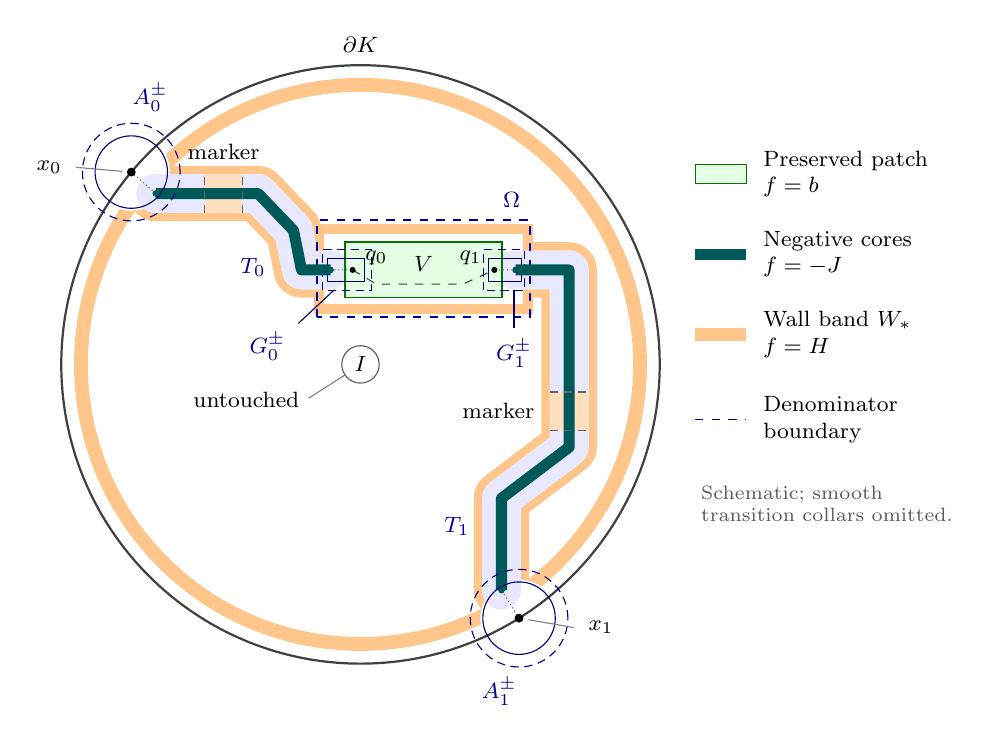
\begin{tikzpicture}[x=1cm,y=1cm,font=\footnotesize,
  forcing label/.style={align=left,inner sep=2pt},
  forcing tube/.style={line width=14pt,line join=round,line cap=round},
  forcing wall/.style={draw=orange!45,line width=20pt,
    line join=round,line cap=round},
  forcing core/.style={draw=teal!70!black,line width=4pt,
    line join=round,line cap=butt}]
  \coordinate (Xzero) at (140:3.8);
  \coordinate (Xone) at (302:3.8);
  \coordinate (Rzero) at (-2.60,2.17);
  \coordinate (Rone) at (1.791,-2.867);
  \coordinate (Szero) at (-.38,1.20);
  \coordinate (Sone) at (1.97,1.20);

  \draw[draw=orange!45,line width=5pt] (0,0) circle (3.55);
  \draw[forcing wall] (Rzero) -- (-1.3,2.17) -- (-.85,1.70)
    -- (-.75,1.20) -- (Szero);
  \draw[forcing wall] (Rone) -- (1.791,-1.7) -- (2.65,-1.05)
    -- (2.65,1.20) -- (Sone);
  \filldraw[fill=white,draw=orange!45,line width=5pt]
    (-.50,.73) rectangle (2.10,1.70);
  \foreach \p in {Xzero,Xone} {\fill[white] (\p) circle (.49);}
  \draw[forcing tube,white] (Xzero) -- (Rzero) -- (-1.3,2.17)
    -- (-.85,1.70) -- (-.75,1.20) -- (Szero);
  \draw[forcing tube,white] (Xone) -- (Rone) -- (1.791,-1.7)
    -- (2.65,-1.05) -- (2.65,1.20) -- (Sone);
  \fill[white] (-.46,.77) rectangle (2.06,1.66);
  \draw[forcing tube,draw=blue!9] (Rzero) -- (-1.3,2.17)
    -- (-.85,1.70) -- (-.75,1.20) -- (Szero);
  \draw[forcing tube,draw=blue!9] (Rone) -- (1.791,-1.7)
    -- (2.65,-1.05) -- (2.65,1.20) -- (Sone);

  \draw[dashed,blue!65!black,line width=.7pt]
    (-.55,.60) rectangle (2.15,1.83);
  \node[anchor=south east,text=blue!55!black] at (2.15,1.87) {$\Omega$};
  \filldraw[fill=green!10,draw=green!45!black,line width=.7pt]
    (-.20,.85) rectangle (1.80,1.55);
  \node[forcing label,align=center] at (.80,1.28) {$V$};
  \foreach \lo/\hi/\slo/\shi in {-.48/.14/-.42/.05,1.56/2.08/1.63/2.04} {
    \draw[blue!55!black,densely dashed] (\lo,.94) rectangle (\hi,1.46);
    \draw[blue!45!black] (\slo,1.05) rectangle (\shi,1.35);
  }

  \fill[orange!25] (-1.98,1.925) rectangle (-1.50,2.415);
  \fill[orange!25] (2.405,-.84) rectangle (2.895,-.35);
  \draw[forcing core] (Rzero) -- (-1.3,2.17) -- (-.85,1.70)
    -- (-.75,1.20) -- (Szero);
  \draw[forcing core] (Rone) -- (1.791,-1.7) -- (2.65,-1.05)
    -- (2.65,1.20) -- (Sone);
  \draw[black!60,densely dashed] (-1.98,1.925) -- (-1.98,2.415)
    (-1.50,1.925) -- (-1.50,2.415)
    (2.405,-.84) -- (2.895,-.84)
    (2.405,-.35) -- (2.895,-.35);
  \node[anchor=south] at (-1.74,2.48) {marker};
  \node[anchor=east] at (2.33,-.595) {marker};
  \node[anchor=east,text=blue!60!black] at (-1.08,1.23) {$T_0$};
  \node[anchor=east,text=blue!60!black] at (1.51,-2.06) {$T_1$};

  \draw[black!60,densely dotted] (Xzero) -- (Rzero)
    (Xone) -- (Rone) (Szero) -- (-.10,1.20) (Sone) -- (1.70,1.20);
  \draw[black!75,dashed] (-.10,1.20) -- (.20,1.02)
    -- (1.30,1.02) -- (1.70,1.20);
  \foreach \p in {Rzero,Rone,Szero,Sone} {
    \fill[teal!70!black] (\p) circle (1.2pt);
  }
  \fill[black] (-.10,1.20) circle (1.1pt);
  \fill[black] (1.70,1.20) circle (1.1pt);
  \node[anchor=south west,inner sep=1pt] at (.02,1.22) {$q_0$};
  \node[anchor=south east,inner sep=1pt] at (1.58,1.22) {$q_1$};
  \node[anchor=north east,text=blue!55!black] at (-.83,.52) {$G_0^{\pm}$};
  \draw[blue!45!black] (-.79,.52) -- (-.34,.94);
  \node[anchor=north,text=blue!55!black] at (1.95,.43) {$G_1^{\pm}$};
  \draw[blue!45!black] (1.95,.46) -- (1.95,.94);

  \draw[black!75,line width=.8pt] (0,0) circle (3.8);
  \node[anchor=south] at (0,3.84) {$\partial K$};
  \foreach \p in {Xzero,Xone} {
    \draw[blue!55!black,densely dashed] (\p) circle (.62);
    \draw[blue!45!black] (\p) circle (.46);
    \fill[black] (\p) circle (1.6pt);
  }
  \node[anchor=east] at ($(Xzero)+(-.76,.06)$) {$x_0$};
  \draw[black!50] ($(Xzero)+(-.12,.01)$) -- ($(Xzero)+(-.70,.06)$);
  \node[anchor=west] at ($(Xone)+(.76,-.12)$) {$x_1$};
  \draw[black!50] ($(Xone)+(.12,-.02)$) -- ($(Xone)+(.70,-.12)$);
  \node[anchor=south,text=blue!55!black] at ($(Xzero)+(.24,.65)$) {$A_0^{\pm}$};
  \node[anchor=north,text=blue!55!black] at ($(Xone)+(-.25,-.64)$) {$A_1^{\pm}$};
  \filldraw[fill=white,draw=black!65] (0,0) circle (.2375);
  \node at (0,0) {$I$};
  \node[forcing label,anchor=east] at (-.70,-.45) {untouched};
  \draw[black!50] (-.66,-.43) -- (-.19,-.13);

  \filldraw[fill=green!10,draw=green!45!black]
    (4.25,2.30) rectangle (4.90,2.54);
  \node[forcing label,anchor=west] at (5.04,2.42) {Preserved patch\\$f=b$};
  \draw[forcing core] (4.25,1.40) -- (4.90,1.40);
  \node[forcing label,anchor=west] at (5.04,1.40) {Negative cores\\$f=-J$};
  \draw[draw=orange!45,line width=5pt] (4.25,.38) -- (4.90,.38);
  \node[forcing label,anchor=west] at (5.04,.38) {Wall band $W_*$\\$f=H$};
  \draw[dashed,blue!65!black] (4.25,-.70) -- (4.90,-.70);
  \node[forcing label,anchor=west] at (5.04,-.70) {Denominator\\boundary};
  \node[forcing label,anchor=north west,font=\scriptsize,text=black!65]
    at (4.25,-1.47) {Schematic; smooth\\transition collars omitted.};
\end{tikzpicture}
\caption{The fixed geometry in Lemma~\ref{comp:finite-catalogue-construction}.
The preservation patch $V$ and its terminal caps lie inside the denominator
$\Omega$, away from the untouched disk $I$.  Two disjoint polygonal tubes
connect the outer caps at $x_0,x_1\in\partial K$ to opposite faces of $V$.
Their negative cores stop inside the safe caps; the dashed preserved
certificate joins $q_0$ to $q_1$ and remains wholly in $V$.  For $D_f=e^{\xi f}\cdot D$, the wall
band prevents a path of $D_f$-length at most $B$ from crossing the forbidden
gap.  The two marked
cross-sections force every such complete tube passage to approach its
core: the marker has height $H$ outside the core collar.  Exact offset
boundaries and smoothing collars are suppressed.}
\label{fig:forcing-corridors}
\end{figure}


\begin{lemma}[Construction of the finite forcing catalogue]
\label{comp:finite-catalogue-construction}
Let $K=\overline{B_2(0)}$ and
$I=\overline{B_{1/8}(0)}$.  Fix a finite set of Euclidean
configurations of the following type.
\begin{enumerate}[label=(\alph*)]
\item A rectangular preservation patch $V$ and a larger
      rectangular denominator domain $\Omega$ satisfy
      $\overline V\subset\Omega\Subset
      B_{3/2}(0)\setminus\overline{B_{1/4}(0)}$.
      Two endpoint ports lie near opposite faces of the
      rectangle inside~$V$.
\item Disjoint terminal caps
      $G_j^-\Subset G_j^+\Subset\Omega$, $j=0,1$, contain
      those ports.  Each $G_j^-$ also contains a fixed stop
      point $s_j\notin\overline V$, which can approach the
      corresponding face from its outer side.  The caps have
      been chosen by a sufficiently fine finite gridding of
      the rectangle and its two endpoint ports.
\item Disjoint outer caps $A_j^-\Subset A_j^+$ surround two
      separated gridded points of $\partial K$.  A fixed
      point $r_j\in A_j^-\cap\operatorname{int}K$ lies a
      positive distance inside $K$.  The possible exterior
      attachment points $x_j\in\partial K$ lie in a compact
      subset of $A_j^-$.
\end{enumerate}
All indicated containments and separations have strict
Euclidean margins.  The endpoint ports and the terminal stops
can, for example, be obtained by taking a thin collar of a
gridded rectangle and cap boxes straddling its opposite faces.
Fix a finite set $\mathcal B\subset\mathbb R$ of exact
constant shifts.

For each configuration one can choose finitely many fixed
polygonal core domains and marker rectangles as described
below.  Suppose the reference metric $D$ and the chosen
endpoints $q_j$ satisfy the following deterministic bounds,
uniformly for that finite family, with positive numbers
$u,w,e,A,K_*,m_*$ and a modulus $\omega(t)\to0$.
\begin{enumerate}[label=(\roman*)]
\item Every point of $A_j^+$ has an old local connection to
      $x_j$ of length at most $e$; there is a connection from
      $x_j$ to $r_j$ in $A_j^-$ of length at most $e/3$.
\item Every point of $G_j^+$ has a $D_b$-connection to $q_j$
      in $\Omega$ of length at most $e$, where
      $D_b=e^{\xi b}D$.  There is a connection from $s_j$ to
      $q_j$ in $G_j^-$ of $D_b$-length at most $e/3$.
\item There is a $D_b$-connection from $q_0$ to $q_1$ inside
      $V$ of length at most $Au$.
\item Each point of the closed core domain can be connected
      to its terminal stop, within that core, at old cost at
      most $K_*w$.  The outer stop has such a connection too.
\item The fixed forbidden-gap and marker crossings have old
      length at least $m_*w$.  Points at Euclidean distance
      at most $t$ from a core can be connected to that core
      inside its prescribed open collar at old cost at most
      $\omega(t)w$.
\end{enumerate}
Fix a local budget $B$ with $Au+2e\le B$.  Then there is a
finite deterministic list of smooth functions $f$, depending
only on the geometric list, these bounds, and $\mathcal B$,
with the following properties.
Each function is supported compactly in
$B_2(0)\setminus I$, is exactly $b$ on $V$, and satisfies
the network, gate, and cheap-approach hypotheses of
Lemma~\ref{comp:gate-forcing} for the indicated configuration
and budget $B$, with all marker-to-terminal joins and the preserved
certificate compactly confined to the bounded neighborhood
$W=B_3(0)$.  It also provides a competitor of cost at
most $\ell_0+\ell_1+B$ whenever the exterior approaches to
$x_0,x_1$ have old costs $\ell_0,\ell_1$.
The list has uniformly bounded amplitudes and Dirichlet
energies, including after any Euclidean translation and
dilation.
\end{lemma}

\begin{proof}
We first make all Euclidean choices; no metric-dependent
curve is used to choose the shape of a shift.

\paragraph{Two embedded corridors.}
Extend the short prescribed initial and terminal pieces to
an arc joining $\partial K$ to the corresponding face of
$\partial V$, inside
$\operatorname{int}K\setminus(I\cup\overline V)$.
Choose the first arc simple.  An arc joining distinct
boundary components of this planar region does not
disconnect its interior after cutting along the arc: the
outer boundary and the rectangular boundary become one
boundary component, while the omitted disk remains another.
Thus the second pair of prescribed ends can be joined in
the cut region.  Approximate both arcs by simple polygonal
arcs, keeping the prescribed short end pieces and positive
clearance from each other, the omitted disk, and the
rectangle except in their terminal caps.  Trim their ends
to obtain disjoint arcs from $r_j$ to $s_j$.

One can require the arcs to avoid the other attachment and
terminal cap by choosing those caps small first.  At a
terminal cap approach along the outward normal to its
specified face.  Since the input configurations form a
finite list, these choices can be made once for each member.
Their minimum positive clearance is then positive.

\paragraph{Nested neighborhoods and the region graph.}
Choose three nested regular neighborhoods
\[
 O^0\subset O^1\subset O^2,\qquad
 N^0\Subset N^1\Subset N^2,\qquad
 T_j^0\Subset T_j^1\Subset T_j^2,
\]
where $O^k$ contains the exterior of $K$ and a thin inner
collar, $N^k$ surrounds $\overline V$, and $T_j^k$ is a
regular tube around the $j$th polygonal arc with end bulbs.
For the unbounded sets $O^k$, require positive separation
between their finite boundary components.
Choose the neighborhoods sufficiently thin that
\[
 \overline{N^2}\subset\Omega,\quad
 O^2\cap N^2=\varnothing,\quad
 T_0^2\cap T_1^2=\varnothing,
\]
and their only overlaps satisfy
\[
 O^2\cap T_j^2\subset A_j^+,
 \qquad N^2\cap T_j^2\subset G_j^+.
\]
All these incidences persist under a further small thickening.
This follows directly from the positive clearances of the
arcs away from their four prescribed end caps.  Make the
end bulbs large enough that the smaller safe caps
$\overline{A_j^-}$ and $\overline{G_j^-}$ lie in the union
of the smallest neighborhoods, with positive margin.
There is no requirement that the larger effective caps be
cheap in the modified metric.

Write
\[
 S^k=O^k\cup N^k\cup T_0^k\cup T_1^k.
\]
These sets avoid a fixed neighborhood of $I$, and there is
$\rho_*>0$
such that the Euclidean $\rho_*$-neighborhood of
$\overline{S^0}$ lies in $S^2$.
The middle layer
\[
 W_*=
 \{z:\rho_*/3\le\operatorname{dist}(z,S^0)
                         \le2\rho_*/3\}
\]
is compactly contained in
$\operatorname{int}K\setminus I$ and disjoint from all
the safe caps and the preservation patch.  A curve starting
in $S^0$ and leaving $S^2$ has a subcurve in $W_*$ whose
endpoints are separated by at least $\rho_*/3$.
This is the forbidden-gap crossing in (v).

The nerve of the cover of $S^2$ by its four regions is
precisely the cycle
\[
 O^2-T_0^2-N^2-T_1^2-O^2.
\]
Any compact curve contained in $S^2$ admits a finite
subdivision subordinate to this open cover and hence a
finite itinerary in that graph.  This statement allows
arbitrarily many incidental boundary contacts.

\paragraph{Core domains and marked sections.}
Choose closed polygonal core domains $C_j\subset T_j^0$
around the trimmed arcs, with the following margins:
\[
 C_j\cap O^2=\varnothing,\qquad
 C_j\cap\overline V=\varnothing,
\]
and both stops $r_j,s_j$ lie in $C_j$.
The outer collar is chosen thinner than the depth of $r_j$;
the inner stop lies outside $\overline V$ by assumption.
The core connection bounds in (iv) concern these fixed
closed domains.  They may be obtained from the internal
box estimates on a finite rectangular cover, including
access to the flat faces.

On a straight interior piece of each polygonal tube, away
from its end bulbs and from $O^2\cup N^2$, select a closed
longitudinal marker rectangle spanning the full closed transverse
section of $T_j^2$ between its two end cross-sections.
The tube there is an
ordinary Euclidean strip.  A path in $T_j^2$ from its outer
overlap to its terminal overlap must cross this rectangle
between two cross-sections a fixed positive distance apart.
One can see this by using the longitudinal coordinate in
the regular tube; retain the subcurve between its last
visit to the first cross-section and its first subsequent
visit to the second.  This is the marker crossing in (v).

\paragraph{A smooth wall and constant plateaux.}
Choose $H>\max\{0,\max\mathcal B\}+1$ so large that
\[
 e^{\xi H}m_*w>B.
\]
Choose a smooth baseline $a$, compactly supported in
$\operatorname{int}K\setminus I$, which is zero on the
safe outer caps and near $\partial K$, equals $b$ on a
neighborhood of $\overline V\cup\overline{G_0^-}
\cup\overline{G_1^-}$, and equals $H$ on a neighborhood
of $W_*$ and on both marker rectangles.  Require also
\[
 a\ge0\text{ on }O^2,
 \qquad a\ge b\text{ on }N^2,
 \qquad \min\{0,b\}\le a\le H.
\]
These requirements have disjoint closed cores and positive
margins.  Explicitly, first choose a cutoff $\zeta$ equal
to one on the preservation patch and the safe terminal
caps, supported in $S^0$ and away from $O^2$, the marker rectangles,
the wall layer, and the safe outer caps.  Next choose
$\psi$ equal to one on $N^2$, the support of $\zeta$,
the marker rectangles, and $W_*$, and zero on the safe
outer caps and near the forbidden support boundaries.
The formula
\[
 a=H\psi+(b-H)\zeta
\]
has all the stated properties, with the cutoffs chosen
between zero and one.

Choose $J>\max\{0,-\min\mathcal B\}+1$ so that
\[
 e^{-\xi J}K_*w<e/3.
\]
Then choose $\rho>0$ smaller than all the fixed geometric
margins, and so small that
\[
 e^{\xi H}\omega(\rho)w<e/3.
\]
Let $\chi_j$ be smooth, equal to one on $C_j$, and supported
in its $\rho$-neighborhood.  These supports are disjoint,
lie inside $S^0$, and avoid $O^2\cup\overline V\cup W_*$.
Set $\chi=\chi_0+\chi_1$ and define
\[
 f=(1-\chi)a-J\chi.
\]
This is a smooth compactly supported shift.  It equals
$-J$ on the cores, $b$ on $V$, and $H$ on $W_*$.  On
the safe terminal caps $f\le b$, and on the safe outer
caps $f\le0$.  Moreover,
\[
 f\ge0\text{ on }O^2,
 \qquad
 f\ge b\text{ on }N^2\setminus(T_0^2\cup T_1^2).
\]

\paragraph{The local budget gives the itinerary.}
A curve starting at $\partial K$ starts in $S^0$.
If a curve of total new length at most $B$ leaves $S^2$,
it crosses $W_*$ and pays more than $B$ by the choice
of $H$.  Thus every local-budget portion between the first
and last visits to $\partial K$ stays in $S^2$.  The
finite-cover argument above gives its claimed itinerary.
The omitted disk supplies no bypass, since it lies outside
$S^2$.  The outer and terminal gate-error conditions follow
from their containments in $A_j^+$ and $G_j^+$ and (i)--(ii).

\paragraph{A marked passage gives cheap endpoint access.}
On a marker rectangle, $a=H$.  Outside the
$\rho$-neighborhood of its core one has $\chi=0$ and
therefore $f=H$.  A complete corridor passage avoiding
that core neighborhood would have an all-wall marker
crossing and cost more than $B$.  Every complete passage
with the local budget consequently contains a point $z$
at distance at most $\rho$ from the core.  By (v), this
point connects to the core at new cost at most
$e^{\xi H}\omega(\rho)w<e/3$.  By (iv), it then reaches
$s_j$ through the core at cost less than $e/3$.  The safe
terminal cap has shift at most $b$, so (ii) gives a final
connection to $q_j$ at cost at most $e/3$.  Thus
\[
 D_f(z,q_j;\text{prescribed neighborhood})\le e.
\]
These marker points supply cheap approach joins.  The
different effective gate contacts are used only for the
old $D_b$ lower-bound corrections in the forcing lemma.
The prescribed core collars and terminal-cap paths lie inside
$B_2(0)$, and the retained certificate lies inside $V$.
Consequently the shortcut assembled from these joins and that
certificate has compact confinement in $W=B_3(0)$.  The outer
region and the long anchor approaches play no part in this
confinement assertion.

\paragraph{The competitor and finiteness.}
Follow the unchanged exterior approaches, the safe outer
cap connections, the negative cores, the safe terminal
cap connections, and the connection through $V$ from (iii).
The six approach contributions have total cost at most
$2e$, so the resulting competitor has length at most
$\ell_0+\ell_1+Au+2e\le\ell_0+\ell_1+B$.

Every region, core, marker, cutoff, and height was selected
from deterministic data after the finite geometric list
and uniform metric bounds had been fixed.  Hence these
functions form a finite list.  Their amplitudes are
bounded by $\max\{H,J,\max_{b\in\mathcal B}|b|\}$.
Smoothness and compact support give a finite common
Dirichlet-energy bound.  Finally,
\[
 \int_{\mathbb C}
 \left|\nabla f\left(\frac{z-z_0}{r}\right)\right|^2
 \frac{dz}{r^2}
 =\int_{\mathbb C}|\nabla f(w)|^2\,dw,
\]
so the energy of $z\mapsto f((z-z_0)/r)$ is unchanged
by translation and positive dilation.
\end{proof}

\begin{remark}[Which bounds are chosen when]
\label{comp:construction-choice-order}
The preservation patch, terminal caps, and their error
bounds are chosen first, followed by the thin-domain
connection bound $A$.  Next choose the fixed ratio $w/u$
large enough for the exterior gap and budget conditions.
The outer attachment grid and all Euclidean tubes are then
fixed.  The new core and gap bounds $K_*,m_*,\omega$ are
truncated on those finitely many domains.  These later
truncations only affect $H,J,\rho$; they do not alter $A$
or the terminal caps.  Thus the construction has no
circular dependence of the upper compartment budget on
the later routing constants.
\end{remark}

\begin{lemma}[Uniform stability for a shrinking modification]
\label{comp:shrinking-modification-stability}
Let $D$ be a proper geodesic metric inducing the Euclidean
topology and having a unique geodesic $P$ between fixed distinct
anchors $a_0,a_1$, parametrized by fractions of its length.
Fix $0<t_1<t_2<1$ and an open set $U$ containing
$P([t_1,t_2])$ with positive clearance.  Suppose the old passage
rule has upper comparison $C$ in open subsets of $U$ and
\[
 F_U(P(t_1),P(t_2))
 =C(t_2-t_1)D(a_0,a_1).
\]
Consider bounded shifts $f$ with one common amplitude bound,
supported in balls whose radii tend uniformly to zero and whose
centers lie at vanishing distance from a fixed compact middle
subarc of $P((t_1,t_2))$.
Let $F'$ be any output passage rule with upper comparison $C$
against $D_f=e^{\xi f}\cdot D$.  Suppose it preserves all old
exterior certificate restrictions outside a slightly enlarged
support ball.  Assume the certificate system permits marked
subpath extraction with additive nonnegative costs and
concatenation with arbitrarily small open loss.

Uniformly over these modifications and all output fillings,
every fractionally parametrized $D_f$-geodesic $P'$ satisfies
\[
 \sup_{t\in[0,1]}D(P'(t),P(t))\longrightarrow0,
 \qquad
 D_f(a_0,a_1)\longrightarrow D(a_0,a_1),
\]
and
\[
 \frac{F'_U(P'(t_1),P'(t_2))}
 {(t_2-t_1)D_f(a_0,a_1)}\ge C-o(1).
\]
If a strict shortcut along $P'$ is contained in the shrinking
modification neighborhood, then for all sufficiently small
supports this ratio is strictly less than $C$.
\end{lemma}

\begin{proof}
Choose constants $0<m\le1\le M<\infty$ with
$mD\le D_f\le MD$.  Properness puts all the relevant geodesics
in one compact $D$-ball.  Let $\omega_n$ be the supremum of the
old $D$-diameters of suitably enlarged possible support balls.
The Euclidean radii tend uniformly to zero, so continuity gives
$\omega_n\to0$.

Replace the portion of an old geodesic between its first and
last support visits by an old minimizing connection.  Its new
length is at most $M\omega_n$.  For the reverse comparison,
cut a new geodesic at its first and last support visits and
insert an old minimizing connection of cost at most
$\omega_n$.  Outside the support the lengths coincide.  Thus
\[
 |D_f(x,y)-D(x,y)|\le(M+1)\omega_n
\]
for the endpoints under consideration.  Moreover, the new
geodesic segment spanning all its support visits has new length
at most $M\omega_n$, and old length at most
$m^{-1}M\omega_n$.  Hence the old length of the entire new
geodesic tends to $D(a_0,a_1)$.

The new geodesics are uniformly Lipschitz in $D$ under their
fractional parametrizations.  Every subsequential limit is an
old minimizing path; equivalently, the uniform distance
comparison shows that each of its subsegments has the
appropriate fractional distance.  Uniqueness identifies the
limit with $P$ with its specified parametrization.  A
contradiction-subsequence argument proves uniformity over all
support locations and bounded shifts.  Write the uniform
endpoint discrepancy as $\eta_n\to0$.

Put $q_0=P(t_1)$, $q_1=P(t_2)$ and
$q'_0=P'(t_1)$, $q'_1=P'(t_2)$.  Consider an arbitrary
output certificate from $q'_0$ to $q'_1$ compactly in $U$.
If it enters the modification neighborhood, cut its
approximants at their first and last visits to a ball strictly
larger than the ball removed from the preserved exterior
patch.  Marked subpath extraction gives retained prefix and
suffix certificates in that open exterior patch, with total
cost no larger than the original cost.  Transfer them to the
old sample.  Join their cut points at old passage cost at
most $C\omega_n+o(1)$, and correct the two endpoints at total
cost at most $2C\eta_n+o(1)$.  All corrections lie in $U$,
by its clearance and the fact that short old geodesics remain
in small neighborhoods.  For a certificate avoiding the
larger ball, transfer it directly and make only the endpoint
corrections.  The retained pieces use their own positive
clearance from $\partial U$; a common clearance for all
competing certificates is unnecessary.

Taking infima yields, with
$\ell=(t_2-t_1)D(a_0,a_1)$,
\[
 C\ell\le F'_U(q'_0,q'_1)+C(\omega_n+2\eta_n).
\]
The new denominator $\ell'$ tends to $\ell>0$, proving the
ratio bound.  Finally, the old middle subarc is separated
from $P([0,t_1]\cup[t_2,1])$.  Uniform convergence therefore
places every visit of $P'$ to the shrinking modification
neighborhood strictly between $t_1$ and $t_2$.  Concatenating
the strict shortcut with upper-comparison paths along the
remaining geodesic portions gives the strict upper inequality.
\end{proof}

\begin{remark}[Deterministic errors before counting]
\label{comp:deterministic-stability-errors}
The error in Lemma~\ref{comp:shrinking-modification-stability}
is a random function of the incoming sample, uniform over all
candidate modifications.  Its almost sure convergence to zero
allows a deterministic sequence $\epsilon_N\to0$ for which
the error exceeds $\epsilon_N$ with probability tending to
zero.  Intersect the event that the error is at most $\epsilon_N$ with
the positive-probability saturation event and the every-point
good-cover event before
forming the source submeasures.  A positive lower cutoff for
the interval length ensures that the ratio error is controlled.
This gives the deterministic common-law sets $H_N$ required
by Lemma~\ref{comp:weighted-output-multiplicity}.
\end{remark}

It remains to make a successful catalogue available with high
probability in a reference shell.  When the passage kernel uses the
genuine order of the local imaginary traversals, an independent trial
must determine that order from its own dependency disk.  The next lemma
provides such disks; for an order-free kernel this step is unnecessary.

\begin{lemma}[A locally certified imaginary order]
\label{comp:local-order-certificate}
Let $\widehat h$ be the whole-plane imaginary field modulo its
angular period, and let $\eta$ be its Lebesgue-parameterized
space-filling curve.  Fix a compact set $K\Subset U$, with $U$
bounded and open.  The following public properties suffice:
\begin{enumerate}[label=(\roman*)]
\item the rational-point visit times of $\eta$ are dense;
\item its full directed $U$-traversals indexed by rational points,
      parametrized by Lebesgue area from their entry times,
      are determined from $\widehat h$ on an arbitrarily small
      enlargement of $U$, and the same holds for bounded disks;
\item each rational spatial point is visited once almost surely.
\end{enumerate}
There are events $D_R$, measurable from the imaginary field on
a slightly enlarged ball of radius $R$, such that
$\mathbb P(D_R)\to1$ and, on $D_R$, the genuine order of all
$U$-traversals meeting $K$ is determined by that restriction.
\end{lemma}

\begin{proof}
Transience confines the visits to $\overline U$ to a compact
time interval.  Uniform continuity gives a positive lower
duration for each $U$-traversal reaching $K$, because it must
cross $\operatorname{dist}(K,\partial U)>0$.  There are
therefore only finitely many such traversals.  Property (i)
ensures that each contains a rational-point visit.  In the
locally reconstructed collection select the first rational
representative in a fixed enumeration for each traversal;
this selection does not use their chronological order.

Apply (ii) again to the disk $B_R$.  For every selected rational
representative, reconstruct its full directed $B_R$-traversal,
with time zero at entry.  Let $D_R$ be the event that all these
records are identical.  It is measurable from the buffered
imaginary-field restriction.  Distinct traversal intervals cannot
have identical records: they have positive time length and hence
positive area, whereas ranges of disjoint time intervals overlap
in zero area.  On $D_R$, the common directed parametrization and
(iii) specify the order of the representatives exactly, and therefore
the order of their distinct small-domain traversals.

Almost surely the finitely many representative visit times have a
finite minimum and maximum.  By continuity, the image of the
interval between them is compact and lies in $B_R$ for all
sufficiently large $R$.  They then lie in one common $B_R$-traversal,
so $D_R$ holds eventually.  This proves the exhaustion.
\end{proof}

\begin{remark}[Public inputs for the preceding lemma]
Properties (i) and (ii) are given in Section~2.1.3 and
Lemma~2.4 of Gwynne--Miller--Sheffield
\cite{GwynneMillerSheffieldHarmonic}.
For (iii), area parametrization makes the set of multiply visited
spatial points Lebesgue-null: cover pairs of distinct visit times
by disjoint rational time intervals, whose ranges have zero-area
intersection.  Translation invariance of the whole-plane curve
modulo time translation then gives zero probability that any fixed
spatial point is multiply visited, and a countable intersection
handles rational points.  The stationary angular-phase convention
for the imaginary field is used here.
The argument uses density of rational \emph{visit times};
positive area of an excursion range alone would not imply
that it contains a rational point.
\end{remark}

\begin{proposition}[Conditional availability of a finite catalogue]
\label{comp:conditional-catalogue-availability}
Consider favorable normalization indices $v$ and a family of
passage kernels.  Suppose:
\begin{enumerate}[label=(\roman*)]
\item For each open preservation patch $V$, the restricted
      certificate kernel is a function of $h|_V$, the local
      imaginary traversal data, and their finite genuine
      order.  The order depends only on the imaginary field,
      and the kernels are compatible under restriction to
      smaller open patches.  Separated restrictions have
      conditional product kernels.
\item Under a common normalized background-field law, at every
      favorable index there is probability at least $\beta>0$
      of a strict low-ratio certificate whose entire range lies in
      a retained closed rectangular envelope and whose endpoints
      lie on its opposite faces, with
      common geometric slack and a denominator in a fixed
      buffered domain.  The fixed reference-metric moduli and
      finite-domain connection bounds are almost surely finite.
\item The exact affine and volume-normalization identities of
      the joint kernel family transport each trial to the
      corresponding favorable reference index after its real
      coarse constant, spatial logarithm, and fixed volume
      displacement have been compensated.  These are identities
      of transported fields and deterministically normalized
      observations, not a Weyl rule for a fixed passage object.
\item The normalized GFF harmonic profiles, after removing the
      real coarse constant and reducing the imaginary constant
      modulo its period, have uniformly tight interior smooth
      norms on fixed-ratio buffered trial disks.
\end{enumerate}
For every $\theta>0$, one can choose finitely many disjoint
buffered trials, a finite deterministic grid of exact real
shifts, and the metric bounds for a finite forcing catalogue
so that, uniformly over favorable indices, the completed
catalogue is available with probability at least $1-\theta$.
The good event can include fixed bounds on all the resulting
Cameron--Martin pairings.  No continuity of passage costs under
rounding a field shift is required.
\end{proposition}

\begin{proof}
First truncate the normalized small-box and face modulus at
a loss smaller than $\beta/10$.  Choose a small mesh width $t$
using this common internal box modulus and the prescribed terminal
error budget.  Grid both the closed-envelope parameters and the
positions of the two endpoints.  For each resulting finite bin,
choose an outward rectangular preservation collar $V$ containing
every envelope in the bin with positive margin.  Each indicated
face of $V$ is within $O(t)$ of the corresponding envelope face.
Choose terminal caps of diameter $O(t)$ straddling these two faces,
containing the endpoint bins and fixed stop points outside
$\overline V$.  The internal box modulus on their collars gives
the desired arbitrarily small terminal connection errors.
The entire certificate range is in $V$ because it was retained
inside its closed envelope.  Choose an intermediate denominator
domain containing $\overline V$ inside the original one.
Its intrinsic denominator is at least the old denominator, so the
strict low-ratio bound remains valid.

The possible endpoints lie in deterministic compact subsets
of finitely many newly thin domains.  Their internal reference
connection diameters are finite almost surely.  Fix an upper
bound $A'$ with a further loss smaller than $\beta/10$.
These cap sizes, thin domains, and $A'$ remain fixed during
all later tube truncations.

For a singleton order input, take its determination event to be
the whole sample space.  Otherwise choose a compact $K\Subset U$
covering the prepared local traversals.  By
Lemma~\ref{comp:local-order-certificate}, a fixed imaginary buffer
makes the sum of order-determination failure probabilities over
the finite geometry bins smaller than $\beta/10$.
Write $E_{v,a}$ for the prepared success event in
bin $a$ at favorable index $v$, intersected with its determination
event, and put $E_v=\bigcup_a E_{v,a}$.  The genuine order on each
of these events is a function of the buffered imaginary field.
Thus the success union $E_v$ is local and retains a common positive
probability, say $\beta_1$.  No individual bin is required to have
positive probability.

Choose a larger fixed conditioning disk around the complete
dependency region.  Local absolute continuity transfers the
reference fields to a pair of Dirichlet GFFs on this disk,
restricted to its interior.  The field density is independent
of the index.  Truncate this single density to conclude that
the success union $E_v$ has probability at least
$\beta_2>0$ under this fixed Dirichlet reference law, uniformly
in the index.

For an affine trial copy, condition on the fields outside its
conditioning disk.  The fields inside are Dirichlet fields
plus exterior-measurable harmonic functions.  On an acceptable
profile event, subtract the real coarse constant and reduce
the imaginary constant modulo its period.  Smooth cutoffs
extend the remaining profiles on the dependency region to
Cameron--Martin functions of uniformly bounded energy.
The same remains true after adding any real residual constant
in~$[-1,1]$.

Let $P$ be the fixed Dirichlet reference law, including an
independent auxiliary kernel seed, and $Q$ one such
conditional law.  The passage kernel is the same function of
the field inputs under both laws.  A uniform inverse
likelihood second moment gives, for the success union $E_v$,
\[
 \beta_2^2
 \le Q(E_v)\,\mathbb E_Q\left[
           \left(\frac{dP}{dQ}\right)^2\right],
 \qquad Q(E_v)\ge\beta_*:=\beta_2^2/K_*>0.
\]
The profile cutoff and $\beta_*$ are independent of the number
of trial copies: the normalized domains and buffer ratios are
fixed, and (iv) controls their harmonic oscillations uniformly.

Choose that cutoff so the expected fraction of unacceptable
profiles is below $\theta/100$.  Markov's inequality implies
that at least half the trials are acceptable except with
probability at most $\theta/50$.  Choose $J$ with
\[
 (1-\beta_*)^{J/2}<\theta/10,
\]
and pack $J$ deterministic disjoint copies of the entire
conditioning disk into the prescribed shell subregion.
All spatial ratios are now fixed.  Before choosing $M$, allocate a
fixed portion of the remaining failure probability to the outer
reference shell: fix a positive normalized crossing lower bound
$a$, a finite boundary-connection upper bound, and a reference
connection modulus there.  The normalized reference field law and
shell geometry are fixed, so these choices do not depend on $M$.
Write $\varepsilon$ for the already fixed normalized terminal error
budget.  Choose the fixed quantum separation $M$ required by the forcing
budget, using this $a$, the already fixed $A'$ and cap errors;
in particular impose $A'+4\varepsilon<aM^p$ in the units of
Lemma~\ref{common:forcing-verification}.  Assumption (iii) absorbs
its logarithmic displacement into the desired compensation,
so it does not change $\beta_*$.

The $J$ desired compensations are exterior-measurable.  Their
normalized vector is uniformly tight: the favorable index
cancels in (iii), leaving only the fixed affine charts, their
coarse field values, and the now fixed displacement from $M$.
Truncate this vector to a compact interval with loss at most
$\theta/10$, and cover that interval by a finite grid
$\mathcal B$ of mesh at most two.  Select the nearest grid
point using only exterior data.  Its residual lies in
$[-1,1]$, precisely the range in the preceding likelihood
bound.

For every exact $b\in\mathcal B$, draw a fresh auxiliary
observation array for the prepared patches from the common kernel
at the exactly shifted real field, and restrict it to each $V$.
Use independent
seeds across disks and grid values, conditional on the fields.
For the selected grid point declare success on the union of its
events $E_{v,a}$; select the first successful bin in the fixed
finite ordering.  On that bin's determination event the genuine
order equals the locally computed order.  Hence the success indicator is
a function of that disk's field restriction, its independent
seed, and the exterior-measurable grid choice.  The indicators
are conditionally independent given the exterior of the
disjoint disks.  Each acceptable disk has success probability
at least $\beta_*$, and the chance of no success is at most
$(1-\beta_*)^{J/2}$.

The successful certificate is kept at the exact grid value
at which it was drawn.  Rounding has been handled by changing
the field law in a uniform absolute-continuity estimate;
no claim about persistence of an individual certificate under
rounding has been made.

Finally impose the remaining regularity and finite internal bounds
for all the gridded routing, core, gap, and access domains, with total additional
failure smaller than the unused portion of $\theta$.
These later bounds affect only the wall and core heights and
the smoothing widths.  They do not change the cap modulus
or $A'$.  After the resulting finite smooth recipe list is
fixed, truncate its finitely many Gaussian linear pairings.
For a smooth compactly supported recipe, this linear functional is a
distributional pairing against its Laplacian, so it depends only on
the real field on the recipe support.  Clipping is therefore part of
the same local shell event.  The uniformly bounded energies give a
fixed clipping threshold with arbitrarily small failure.  Allocating the
remaining losses proves the claimed probability.
\end{proof}

\begin{remark}[The real and imaginary dependency patches differ]
\label{comp:separate-field-dependencies}
The larger order buffer in the preceding proof is an
\emph{imaginary}-field dependency region.  A real-field
modification leaves this input unchanged.  By the restriction
compatibility in assumption (i), a retained certificate
compactly in $V$ uses the real field only on $V$, even if it
was originally sampled as part of a larger auxiliary passage
object.  Thus a recipe equal to $b$ on $V$ retains precisely
the required kernel after modifying the real field elsewhere.
The reference-metric denominator in a larger domain is used
for the deterministic lower bound and need not be retained
as an unchanged output passage observation.

This use of restriction compatibility is the reason the real and
imaginary dependency patches are specified separately.
\end{remark}

\begin{proposition}[Rigidity from local forcing]
\label{comp:rigidity-implication}
Suppose the comparison family satisfies the hypotheses of
Proposition~\ref{comp:equality-tangent}.  Assume in addition that the
positive-probability rectangular shortcuts can be amplified to a
high-probability shell event with a finite deterministic catalogue
satisfying Lemma~\ref{comp:gate-forcing}.  The event must include the
following data, with constants independent of the scale:
\begin{enumerate}[label=(\alph*)]
\item regular upper and lower reference bounds of order
$w=(M\lambda^{-i})^p$, and a shortcut with denominator in
$[a'\lambda^{-ip},A'\lambda^{-ip}]$;
\item shifts of uniformly bounded amplitude and Dirichlet energy,
constant on the complete real-field dependency patch of the retained
shortcut, vanishing on the preserved exterior patch;
\item the likelihood clipping of
Lemma~\ref{comp:restricted-cm-transfer}, imposed before applying
Lemma~\ref{comp:ann-coverage};
\item output-observable shell traversal events with a lower reference
cost $\kappa w$ and the bounded overlap and alignment multiplicities
in Remark~\ref{comp:counting-checks}.
\end{enumerate}
Assume the exact local product kernels permit the completion and
preservation in Lemma~\ref{comp:restricted-cm-transfer}.
Then the optimal comparisons coincide, $c=C$, and
$F_U=CD_U$ for every open $U$.
\end{proposition}

\begin{proof}
If $c<C$, take the equality tangent and the positive-probability event
in Equation~\eqref{comp:fixed-saturation}.  Restrict its interval length
below by a deterministic positive number and its total anchor length
above by a deterministic finite number; some such restriction still
has positive probability.  Apply Lemma~\ref{comp:ann-coverage} to the
favorable finer labels given by Proposition~\ref{comp:amplification},
with volume multiplier $M$ and with the full good event (a)--(c).

On the retained middle subarc, every point lies in at least $\beta N$
good holes.  A good ball accounts for at most $K_0w$ of geodesic length:
the time span between its first and last visits is bounded by a
reference boundary connection, since a geodesic minimizes between
any two of its points.  Integration over the subarc gives
\[
 \sum_{\text{good hit balls}}w\ge K_0^{-1}\beta N
       \operatorname{len}_D(\text{middle subarc}).
\]
Choose a recipe by a fixed ordering among the successful members of
the finite catalogue.  This partitions source events and adds no
probability conditioning factor.  Intersect with the deterministic
uniform-error events of
Remark~\ref{comp:deterministic-stability-errors}; their lost probability
tends to zero.  The expected source weight is still at least
$\alpha_0N$ for some $\alpha_0>0$.

For each deterministic candidate index, perform its fixed shift and
complete the passage law before restricting to the selected source
event.  Lemma~\ref{comp:restricted-cm-transfer} gives an output
submeasure $\nu_\beta\le\Lambda\mu$ with the same fixed common law
$\mu$.  Gate forcing gives a strict shortcut on the output geodesic.
Shrinking-modification stability puts the gain in the same fixed
fractional interval and shows that the output ratio from Equation~\eqref{comp:output-ratio}
belongs to
\[
 H_N=\{C-\epsilon_N\le R<C\},\qquad \epsilon_N\downarrow0.
\]
Here $R$ is the same function of the output fields and passage data,
and $\mu$ is the common dominating law.

The output traversal tests in (d), bounded overlap at each spatial
radius, $O(N)$ radii, and boundedly many aligned labels and recipes
give total output weight at most $K_1N$ times its anchor length.
The source length cutoff and the common amplitude bound give a
deterministic output length cutoff.  Thus the hypotheses of
Lemma~\ref{comp:weighted-output-multiplicity} hold and force
$\mu(H_N)\ge\alpha_0/(\Lambda K_2)>0$.  Bounded convergence gives
$\mu(H_N)\to0$, a contradiction.

We have $c=C>0$.  The upper bound is
Equation~\eqref{comp:upper-internal}, and the lower bound follows from
Lemma~\ref{comp:intrinsic-lower}.  Therefore $F_U=CD_U$.
\end{proof}

The catalogue-availability hypothesis in
Proposition~\ref{comp:rigidity-implication} combines
Proposition~\ref{comp:conditional-catalogue-availability} with
Lemma~\ref{comp:finite-catalogue-construction}.  The real-field dependency
patch must fit inside the denominator collar: preserving a shortcut
on a much larger constant-shift patch could allow a bypass around
that collar.  An enlarged imaginary-field buffer is harmless because
the imaginary field is unchanged.  This distinction is part of the
local-kernel requirement in this application.

\begin{lemma}[Verification of the forcing hypotheses]
\label{common:forcing-verification}
Let a family satisfy Definition~\ref{common:admissible}, the reference
metric inputs above, and the finite positive comparison hypotheses of
Proposition~\ref{comp:equality-tangent}.  Then its equality tangent
satisfies the catalogue, clipping, completion, and output-count
hypotheses of Proposition~\ref{comp:rigidity-implication}.
\end{lemma}
\begin{proof}
The low event is Proposition~\ref{comp:amplification}(ii), with its
closed rectangular envelope and actual internal denominator metric.
The kernel restriction and product properties give condition (i) of
Proposition~\ref{comp:conditional-catalogue-availability}; in the
one-order case its local order event is the whole sample space.
Otherwise Definition~\ref{common:admissible}(vi) and
Lemma~\ref{comp:local-order-certificate} provide that event using a
larger imaginary buffer.  The exact volume and affine identities give
condition (iii), and Lemma~\ref{common:disk-profiles} gives condition
(iv).  The reference internal box and face bounds give condition (ii).
Thus the complete local catalogue, including fresh observations at each
exact shift and likelihood clipping, has probability as close to one
as required by Lemma~\ref{comp:ann-coverage}.

We verify explicitly how a hit of the old reference geodesic supplies
the deterministic forcing data.  Write $u=\lambda^{-ip}$ and
$w=M^p u$.  Include in the good event a lower reference crossing bound
$aw$ between the central hole and the outer circle, a surrounding
boundary connection bound $Aw$, and fixed reference connection moduli.
On a deep hit, the reference geodesic pays at least $aw$ between first
entry and last exit from the outer circle.  Its exterior pieces pay
at least the two exterior infima $\ell_0,\ell_1$.  Hence
\[
 D(a_0,a_1)\ge\ell_0+\ell_1+aw.
\]
Its exterior minimizing landing points have reference distance at
least $aw$, by concatenating their exterior approaches.  The truncated
reference modulus separates them by a fixed positive Euclidean amount,
so they fit a finite outer-cap grid with the required small errors.

Let the prepared low denominator satisfy $d\ge a'u$.  Choose
$e=\varepsilon u$ with $4C\varepsilon<\delta_0a'$.  The thin
preservation patches, terminal caps, and their connection bound $A_1u$
have already been fixed in the catalogue-availability proof.  Choose
the fixed $M$ so large that
\[
 A_1u+4e<aw,
 \qquad B=A_1u+2e.
\]
All later core, gap and access bounds concern a finite family of
new domains and affect only wall heights, core heights and smoothing
widths.  Lemma~\ref{comp:finite-catalogue-construction} therefore
applies without changing $A_1$ or the terminal errors.  Its budget and
gate conditions give $B+2e<aw$ and $4Ce<\delta_0d$, precisely the
strict inequalities of Lemma~\ref{comp:gate-forcing}.
The resulting strict shortcut has compact confinement in the image
of $B_3(0)$ around the hit ball.  These neighborhoods shrink uniformly
to the old compact middle subarc and eventually lie in its fixed
saturation neighborhood $U$.

Fix the Gaussian pinning circle outside that neighborhood and all
the late candidate supports, as in the equality-tangent proof.
Every deterministic recipe is then a Cameron--Martin direction of
this same actual Gaussian law.  Its real shift is constant on the
complete preservation patch and vanishes on the preserved exterior
patch; the larger imaginary buffer is unchanged.  Resample the local
area marks with their shifted intensity.  The conditional product
kernel and standard Borel completion in
Definition~\ref{common:admissible} give exactly the unselected
construction of Lemma~\ref{comp:restricted-cm-transfer}.  Its finite
Gaussian pairing cutoffs are part of the catalogue event before
annulus coverage or a geodesic hit is selected.

For clarity, the required output count can use a shell where the
shift is identically zero.  Include among the local reference tests
a lower bound $\kappa w$ for every crossing of
$B_{3r}(z)\setminus\overline{B_{2r}(z)}$.
Every forced reference geodesic enters the compartment inside
$B_{2r}(z)$ from anchors outside $B_{4r}(z)$, and crosses this
unchanged shell.  Its output length inside $B_{4r}(z)$ is therefore
at least $\kappa w$.  Define the output event by this length bound,
the inherited deterministic anchor-length cutoff, and the alignment
condition on the outer circle average.  That average is unchanged
by the recipe supported in $B_{2r}(z)$, so every generated output
satisfies the event.  These are functions only of the output field,
its fixed-anchor geodesic and the deterministic candidate index.

For each fixed ball, alignment allows at most
$2+\lceil2L/\log\lambda\rceil$ volume labels, and there are only
finitely many recipes.  The center mesh has bounded overlap at each
radius, and Lemma~\ref{comp:ann-coverage} uses $O(N)$ radii.
Charging the output event's weight to its geodesic length in
$B_{4r}(z)$ thus bounds the total output weight by a constant times
$N$ times the output anchor length.  The source length cutoff and
uniform shift amplitude bound this last length deterministically.
This proves (d) of Proposition~\ref{comp:rigidity-implication}; the
preceding paragraphs prove (a)--(c) and its completion hypothesis.
Uniform stability follows from
Lemma~\ref{comp:shrinking-modification-stability}.
\end{proof}

\begin{theorem}[Identification of local passage laws]
\label{common:identification}
Fix $\gamma\in[\sqrt2,2)$ and $\lambda>1$.  Let a family of local
passage laws satisfy Definition~\ref{common:admissible} and the
reference metric inputs stated above.  Suppose a law in this family
has a finite positive deterministic optimal upper comparison
$0<C<\infty$, with its comparison bounds retained at its fixed
quantum offsets and further extractions.  Then its optimal lower
comparison equals $C$, and
\[
 F_U(x,y)=C D_h(x,y;U)
\]
on every ordinary open chart $U$, with compact confinement and
exhaustion as above.  The multiplier $C$ is deterministic for the
entire joint law.  This theorem gives no estimate for a prescribed
discrete endpoint.
\end{theorem}
\begin{proof}
If the lower optimal constant $c$ were smaller than $C$, the common
annulus lemma, comparison transport, and amplification would give the
equality tangent of Proposition~\ref{comp:equality-tangent}.
Lemma~\ref{common:forcing-verification} supplies every additional
hypothesis of Proposition~\ref{comp:rigidity-implication}, whose
weighted output argument is a contradiction.  Thus $c=C>0$.
The intrinsic lower bound is Lemma~\ref{comp:intrinsic-lower}; the
upper bound follows from continuum joining and port comparison,
as in Equation~\eqref{comp:upper-internal}.  Countable compact
exhaustion gives the simultaneous assertion on open charts.
The constants in Equation~\eqref{comp:optimal-constants} are
deterministic properties of the whole law; proving them equal is
what excludes an additional sample-dependent multiplier.
\end{proof}

\begin{proposition}[Two-sided shell tests control relative units]
\label{comp:relative-units}
Work in the physical passage and annulus-transfer framework of
Definition~\ref{common:admissible} and Lemma~\ref{comp:ann-coverage}, with
the comparisons of Corollary~\ref{comp:annulus-comparison} available.
Let $G_i$, $i\ge i_0$, be own-unit rules with positive deterministic
normalization coefficients $b_i$. Assume that, for every base $i$, its
actual relative-offset laws under the intrinsic transport and quantum-unit
identities \eqref{comp:ann-index-definition}--\eqref{comp:ann-two-units}
are $(b_{i+\ell}/b_i)G_{i+\ell}$ in the base $i$ reference units.
In particular these are the conditional kernels on the physical annuli
to which the annulus-transfer estimates apply.
Suppose every $G_i$ satisfies, with
probability above the annulus transfer threshold, fixed shell tests
with constants $0<m<M<\infty$: lower crossing bounds $m$ for the
passage rule and reference metric, surrounding upper bounds $M$ for
both, and an upper crossing bound $M$ for each with endpoints to which
the other's lower bound applies. Then there is $T<\infty$, depending only on $m,M$
and the fixed geometry, such that
$T^{-2}\le b_i/b_j\le T^2$ for all $i,j\ge i_0$.
\end{proposition}

\begin{proof}
Take $T>4(1+M/m)^2$, increasing it for any fixed geometric enlargement.
If at least one quarter of the labels in arbitrarily late windows
satisfy $b_{i+\ell}>Tb_i$, their passage lower bounds are $mTw_\ell$.
The reference upper bounds are $Mw_\ell$.  Annulus transfer and
Corollary~\ref{comp:annulus-comparison} give the deterministic lower
comparison $G_i\ge(mT/M)D$.  The base shell test has positive probability
of a passage crossing of cost at most $M$ and reference distance at
least $m$, contradicting $m^2T/M>M$.

If one quarter instead satisfy $b_{i+\ell}<b_i/T$, the same argument
in the other direction gives upper comparison $M/(mT)$.  A base
reference crossing of length at most $M$, whose passage crossing cost
is at least $m$, gives the same contradiction.  Thus each of these two
exceptional sets has fewer than one quarter of the labels in all
sufficiently late windows.  Lemma~\ref{comp:majority-ratios} concludes
the proof.  Almost-sure comparisons are obtained by choosing a
subsequence of annulus windows with summable failure probabilities,
and then exhausting countably many buffered tests.
\end{proof}

\begin{lemma}[Overlap of one-sided density bounds]
\label{comp:majority-ratios}
Let $b_i>0$ and $T>1$.  Suppose that, for each fixed $i$, for all
sufficiently large $N$, each of the sets
\[
 \{k\in[i+N,i+2N]:b_k>Tb_i\},\qquad
 \{k\in[i+N,i+2N]:b_k<b_i/T\}
\]
has fewer than $(N+1)/4$ elements.  Then $T^{-2}\le b_i/b_j\le T^2$
for every $i,j$.
\end{lemma}

\begin{proof}
For large $N$, the windows based at $i,j$ have $N-O(|i-j|)$ common
indices.  In their overlap, the conditions $b_k\le Tb_i$ and
$b_k\ge b_j/T$ have a common index, since their excluded sets together
have fewer than $(N+1)/2$ elements.  Hence $b_j\le T^2b_i$.
Interchange $i,j$.
\end{proof}

\section{Circuit normalization for critical FK maps}
\label{comp:fk-normalization-section}

We now return to the fixed FK parameter $q\in(0,4)$ and use the
quantum volume base $\lambda=4$.  Our deterministic distance denominator
will be a quantile of the length of a circuit surrounding the cone mark.
This circuit test has no prescribed lattice endpoint.  Lower crossing
tests first produce record scales whose earlier quantiles have the
reference power-law upper bound in the limit.  Annulus comparison and
rigidity identify the resulting passage laws.  Their two-sided shell
tests then control the relative cost units, allowing a first-failure
argument to propagate a polynomial ratio bound to all scales.

\subsection{Circuit quantiles and coherent quantum offsets}

Use the circle-average embedding of the Brownian cone, with its mark
at $0$, initially modulo rotations.  Fix three nested buffered winding
bands with strict margins which are concentric round annuli about $0$,
with their coarse-test compact annulus and fixed real-field buffers
contained in $\{1/8<|z|<7/8\}$.  Thus these local tests avoid both
the cone mark and the circle-average pinning circle $|z|=1$.
The following choice
fixes their finite-resolution law once and for all.  Let $P$ be the
bilateral iid raw-word law, and let $\mathsf B$ be the normalized
two-sided Brownian contour law.  For every integer $k\ge0$, choose a
joint law $P_k(dW,dZ^k)$ with marginals $P$ and $\mathsf B$ such that
the resolved contour of $W$, divided by $\sqrt{4^k}$ and viewed at
time unit $4^k$, differs from $Z^k$ by a quantity tending to zero in
probability in the compact-uniform topology.  The invariance principle
and a coupling metric for weak convergence give these choices.  They
are fixed before any quantile or subsequence is selected.

Fix measurable readouts of a Brownian contour for the
intrinsic decorated surface, an arbitrary measurable rotational section
of its circle-average coordinate representative,
its curve, and its field and internal metrics on a countable chart
family.  Only contour-determined readouts are meant here.  Fix also
the deterministic mesh projection convention of
Section~\ref{bg:topology-section}, chosen to commute with rotations,
an ordering of the countably many finite primal circuits, and the open
middle-band winding test.
For example, select vertex representatives by their raw time ordering,
project them by $\eta$, and interpolate a projected edge by a straight
segment; every step of this convention commutes with rotation.
Under $P_k$, project the mesh using the curve readout of $Z^k$.
Define $X_k$ as the least genuine unscaled all-edge length of a
primal circuit whose projected range satisfies this fixed test,
using $\infty$ if the collection is empty.  The first minimizer in
the fixed ordering may be marked.  Countable infima make $X_k$
measurable.  All later appearances of its law refer to this exact
chosen $P_k$ marginal.
The band range and winding requirements are invariant under rotation,
so $X_k$ and its first raw-circuit minimizer do not depend on the chosen
rotational section.  We do not assert that the field in an arbitrary
such section has the standard embedded cone law.

Fix $\alpha\in(0,1)$
and, when $\mathbb P[X_j<\infty]>\alpha$, put
\begin{equation}\label{comp:quantile}
 A_j=\inf\{m\in\mathbb N:m\ge1,\ \mathbb P[X_j\le m]\ge\alpha\}.
\end{equation}
Since the finite costs are integers, this gives
\begin{equation}\label{comp:quantile-slack}
 \mathbb P[X_j\le A_j]\ge\alpha,
 \qquad \mathbb P[X_j<A_j]<\alpha.
\end{equation}
In particular, no continuity of the distribution at its quantile is
required.  The hypothesis \mbox{$\mathbb P[X_j<\infty]>\alpha$} ensures that
this quantile is finite.
Lemma~\ref{comp:fk-coarse-tests} makes the inequality hold for every
sufficiently large $j$; assign arbitrary finite positive values to the
finitely many remaining $A_j$ when defining the normalization sequence.
All quantile-slack arguments below concern the sufficiently large indices.

To compare these quantiles across scales, their defining circuit
variables must occur in one actual word experiment.  The next lemma
preserves each previously fixed marginal while constructing the joint
offset array.  It also retains the field and reference metric in the
same quantum units as the passage observations.

\begin{lemma}[One word and exact offset quantile marginals]
\label{comp:quantile-couplings}
For a sequence of base indices $j\to\infty$, the fixed-offset arrays
can be sampled with one common iid word so that the coordinate at
offset $i$ has exactly the chosen $X_{j-i}$ law.  In every finite
offset family, the auxiliary Brownian contours converge jointly to
the canonical time rescalings of one common contour.  Their actual
joint contour-determined spatial, field and internal-metric readouts
can be retained with this same consistency.
\end{lemma}

\begin{proof}
Sample one word $W\sim P$.  Conditional on that word, draw the entire
countable family $(Z^k)_{k\ge0}$ once from the product of the fixed
kernels $P_k(dZ\mid W)$.  Every offset array reuses the coordinate
$Z^{j-i}$ from this family.  Use the
previously fixed definition of $X_{j-i}$ on that same word and
auxiliary contour.  Its marginal is exactly the one defining the
quantile, even though different offset coordinates are dependent
through $W$.

For $v_i=4^{-i}$, write
$(\mathsf T_i Z)(t)=v_i^{-1/2}Z(v_it)$.  Both $Z^{j-i}$ and
$\mathsf T_i Z^j$ approximate the same resolved word in offset
units.  Thus their compact-uniform difference tends to zero in
probability for every fixed $i$.  A finite union handles any fixed
offset family.  Both arguments of each canonical readout have the
same fixed Brownian marginal.  For a measurable readout into a
Polish space, Lusin's theorem makes it uniformly continuous on a
compact set of marginal probability at least $1-\epsilon$.
Consequently readouts of these two close arguments differ by a
quantity tending to zero in probability, after a loss at most
$2\epsilon$.  Let $\epsilon\downarrow0$, apply the argument to
finite subarrays, and diagonalize over the countable chart family.
This retains the joint field/metric readout, rather than only its
separate marginal laws.  At this stage its arbitrary rotational
sections are identified by quantum-surface equivalence.

The standard residual rotation is now sampled once, uniformly,
independently of the common contour and the entire observation array.
This restores the standard embedded cone law.  The concentric winding
tests, and the Euclidean-advance tests in the concentric compact annulus
used below, are unchanged pointwise; consequently the exact finite
circuit laws and the spatial-advance test laws used in
Lemma~\ref{comp:fk-coarse-tests} are preserved.  An imaginary-field completion
not determined by the contour is likewise adjoined
once, conditional on the entire common limiting contour and this
rotation, independently of the entire actual and reference observation
array under the convention of Proposition~\ref{loc:kernel-closure}.
Its copies at other offsets are transported from that same draw.
More explicitly, let $\phi_i$ map the circle-average representative
at offset $i$ to the common base representative, choosing its orientation
by transport, and put $c_i=\gamma^{-1}\log v_i$.  It is a positive
dilation after this common choice of orientation.  The actual readouts
satisfy
\[
 h_i=h_0\circ\phi_i+Q\log|\phi_i'|-c_i,\qquad
 \eta_i(t)=\phi_i^{-1}\eta_0(v_it),\qquad
 D_i=v_i^{-p}\phi_i^*D_0.
\]
The same identities hold for every internal metric on its transported
domain.  Intrinsic affine covariance of the local kernels then gives
the indexed kernel $\mathcal K_i$ in these units.  These are transported
annuli, which need not coincide as Euclidean sets in the base chart.
In unchanged numerical cost units, if $F_0=CD_0$, the pulled-back
rule satisfies $\phi_i^*F_0=Cv_i^pD_i$.  Thus only the deterministic
quantum-unit factor enters the offset comparison; the random coordinate
dilation supplies no additional normalization.
Unrelated rotations or imaginary-field draws at different offsets
are not used to infer coherence.

The finite variables $Z^k$ serve only to define the quantile and its
projection readouts.  The exact raw-chart resampling identities are
proved before the limiting spatial readout, and no conditional
independence of finite microscopic observations given $Z^k$ is
asserted.  In the limit the contour-determined readouts are the
measurable functions just identified; the additional variables have
the stipulated conditional independence.  These are precisely the
auxiliary-conditioning conditions used by
Proposition~\ref{loc:kernel-closure}.
\end{proof}

Annulus comparison uses local Gaussian field changes.  We next transfer
the indexed passage laws to an outside-pinned Gaussian reference, keeping
their numerical cost units.  The joint offsets then extend the comparison
from ordinary patches of the normalization disk to the whole cone atlas.

\begin{lemma}[Actual Gaussian references and the ordinary cone atlas]
\label{comp:fk-reference-atlas}
The FK local kernels on buffered ordinary patches of the normalized
cone disk transfer to an actual Gaussian field with a fixed pinning
circle outside every observation buffer.  The local field density is
the same for all indexed kernels attached to that field marginal.
If a comparison holds with the same numerical constant for all the
indexed Gaussian laws, it holds on every ordinary cone chart.
Conversely, a strict local improvement on the cone would improve the
Gaussian comparison.  These assertions retain the real additive
constant and the complete joint observation law.
\end{lemma}
\begin{proof}
Inside its normalization disk the cone field is
$G_1-\gamma\log|z|$, where $G_1$ has zero unit-circle average
\cite[Definition~4.10 and the following discussion]{DMS}.
Under the deterministic coordinate map $z\mapsto z/R$, this is
\[
 G_R(z)-\gamma\log|z|+(\gamma-Q)\log R,
 \qquad G_R(z)=G_1(z/R).
\]
On a compact ordinary patch in $B_R\setminus\{0\}$ the displayed
drift has a smooth finite-energy extension supported away from both
$0$ and the pinning circle.  Cameron--Martin gives mutual absolute
continuity with the actual $G_R$ restriction.  To put a prescribed
buffered shell in such a patch, first map it by a fixed positive affine
map into $B_1\setminus\{0\}$.  The pulled-back pinning circle remains
outside the complete buffer; the drift, including $Q\log|\phi'|$,
again has a Cameron--Martin extension.  The pin need not be centered
on the shell.

Any two fixed exterior pins give equivalent restrictions on a smaller
common patch.  Indeed, on an intervening domain $W$ their domain
Markov decompositions have an independent zero-boundary GFF and a
harmonic part.  On $K\Subset W$ each harmonic part admits a
finite-energy cutoff in $W$.  Conditional Cameron--Martin equivalence
with the zero-boundary restriction, followed by integration, proves
the assertion.  No circle average is reset in this comparison.
The independent stationary-phase imaginary field has the same local
law under these affine maps.  Adjoining the same local kernels, with
their genuine order and correct local area marks, preserves each
field density.  If $Z=d\nu/d\mu$, then for any indexed kernel and
event $E$,
\[
 (\nu\otimes\mathcal K_i)(E)
 \le T(\mu\otimes\mathcal K_i)(E)
       +\mathbb E_\mu[Z\mathbf1_{\{Z>T\}}].
\]
The tail is independent of $i$.  Thus uniform probability bounds
transfer by truncating this fixed density; a quantitative exponential
rate under an arbitrary equivalent field law is not asserted.

For the full atlas use the actual common offsets of
Lemma~\ref{comp:quantile-couplings}, including each fixed negative
offset.  Put $c_v=\gamma^{-1}\log v$ and
\[
 r_v=\sup\{r>0:h_r(0)+Q\log r=c_v\},\qquad
 h^{(v)}=h(r_v\,\cdot)+Q\log r_v-c_v.
\]
The circle-average cone law and its quantum scaling
\cite[Proposition~4.13(i)]{DMS} give the original joint background law
at every fixed $v$.  The imaginary field is pulled back from the same
sample; its stationary phase and independence of the real field
preserve this joint law.  The matching raw time, height, cost, and
reference arrays were transformed together before extraction.  Their
intrinsic readouts therefore obey
\[
 F^{(v)}_{U}=v^{-p}\phi_v^*F_{\phi_v(U)},\qquad
 D_{h^{(v)}}(\cdot,\cdot;U)
       =v^{-p}\phi_v^*D_h(\cdot,\cdot;\phi_v(U)),
 \quad \phi_v(z)=r_vz,
\]
and the local kernel in the new units is $\mathcal K^{(v)}$.
These are identities for the transported observations, with fresh
reference kernels identified by Proposition~\ref{loc:kernel-closure}.
They are not field-shift identities for an individual passage sample.

Set $H(r)=h_r(0)+Q\log r$.  The radial cone construction gives
$H(r)\to-\infty$ as $r\downarrow0$, and $H$ is continuous.
Hence $\sup_{0<r\le R}H(r)<\infty$ for each finite $R$.
Since $c_{4^m}\to\infty$, it follows that $r_{4^m}\to\infty$.
For each fixed $m$, the comparisons under the indexed Gaussian kernel
transfer to every ordinary patch inside the normalized cone disk.
Pulling them back cancels the two factors $4^{-mp}$ and covers
$B_{r_{4^m}}\setminus\{0\}$.  A countable intersection over $m$
and a countable chart exhaustion gives the whole ordinary cone atlas.
This uses an exact joint quantum-unit identity, without conditioning
on a random dilation and then applying local absolute continuity.
For the reverse assertion, transfer a local comparison on ordinary
patches of the unit disk to the Gaussian reference by mutual absolute
continuity and intrinsic affine transport.  Lemma~\ref{comp:comparison-transport}
then preserves its numerical constant at every fixed quantum index.
\end{proof}

\begin{lemma}[Noncollapse of a quantile-normalized upper rule]
\label{comp:quantile-noncollapse}
Suppose a sequence normalized by $A_j$ has a certificate limit, winding
realizations pass from the narrow band to the middle band with arbitrary
cost loss, and the limiting rule can follow every rectifiable path at
zero cost with open ports.  If the reference narrow band has a finite
rectifiable surrounding circuit almost surely, these assumptions
contradict Equation~\eqref{comp:quantile-slack}.
\end{lemma}

\begin{proof}
Cover a reference surrounding circuit by finitely many transverse port
tests in the narrow band.  Zero upper comparison gives certificates of
arbitrarily small total cost; robust transverse intersections stitch
them into a primal winding circuit.  Exhaust its finite number of
ports, reference length, and strict margins.  For every $\delta>0$, this
gives, with limiting probability at least $1-\delta$, a middle-band
circuit of cost less than $A_j/2$ for all sufficiently large $j$.
Choose $\delta<1-\alpha$.  Its probability is then strictly greater
than $\alpha$, contradicting
$\mathbb P[X_j<A_j]<\alpha$.
\end{proof}

The preceding lemma excludes a zero upper comparison after an upper
comparison has been constructed.  A single quantile does not by itself
give tight lower band costs, a finite upper comparison, or any estimate
for nearby discrete endpoints.

\begin{lemma}[Concrete finite-resolution tests]
\label{comp:fk-coarse-tests}
Assume the framework's contour coupling, marked certificate extraction,
and robust primal projection topology on compact sets.  The winding
variables $X_j$ can then be chosen so that
$\mathbb P[X_j<\infty]\to1$ and $A_j\to\infty$.
There is a fixed finite collection of compact spatial-advance tests
that satisfies the crossing-test hypotheses of
Proposition~\ref{comp:initial-growth}.
\end{lemma}

\begin{proof}
Keep the three concentric winding bands fixed above, and choose a
concentric compact annulus $K$, bounded away from the cone mark,
containing the widest band in its interior.  Finite disk covers of a
slightly larger annulus supply all required local chart patches.  Choose
$\delta>0$ smaller than the Euclidean diameter forced by winding
around the inner hole.  A deterministic polygonal loop in the
narrowest band has an approximate primal lift by the projection
topology.  Its lift is a finite graph walk, stays in the middle band,
and has nonzero winding.  Extract a simple surrounding subcircuit.
Thus, on the events where the projection error is smaller than the
fixed margins, $X_j$ is finite.  These events have probability tending
to one.  Time windows are first enlarged to contain the preimages of
the annulus; transience gives this with arbitrarily high probability.
No cost bound for the lift is asserted.

Define $Y_j$ to be the infimal number of edges of a primal path whose
projected range lies in $K$ and whose projected endpoints are at
Euclidean distance at least $\delta$.  Use $\infty$ for an empty
collection.  Slightly larger compact confinements and slightly smaller
separations provide strict versions.  The contour coupling and the
closed chord relation make the largest projected diameter of a single
edge tend to zero, uniformly on the relevant compact time windows.
A path of at most $k$ edges has diameter at most $k$ times this
quantity.  Therefore, for each fixed $k$,
$\mathbb P[Y_j\le k]\to0$.  Every winding circuit tested by $X_j$
contains an admissible path for $Y_j$, so $Y_j\le X_j$ and
$A_j\to\infty$.

At any proposed cost unit $b_j$, failure of the test
$\mathbb P[Y_j\ge b_j]\ge1-\eta$ retains, with probability at
least $\eta$, a path of normalized cost at most one and endpoints
separated by at least $\delta$.  The endpoints and range lie in fixed
compact sets.  Marked extraction retains a certificate with that
separation and finite cost.  First choose a sufficiently large time
window that its lost probability is less than $\eta/2$, then pass to
the extraction and exhaust windows.  The fixed spatial margins retain
the separated endpoints and compact confinement.

Choose a buffered annulus inside the interior of $K$ with radial
crossing separation greater than $\delta$.  Its primal traversal
tests are included among these spatial-advance tests.  Translations
and the fixed affine changes needed to place the annulus use a finite
collection of slightly enlarged versions of $K$.  The common local
kernels transfer their high-probability tests to the fixed GFF
reference: the field change of density is fixed, so
Equation~\eqref{comp:ann-reference-change} allows $\eta$ to be chosen
small enough for the annulus threshold.  Uniform bounded-edge advance
gives the required initial runs, and the retained finite-cost witness
gives the required first-failure contradiction.  These are precisely
the test conditions of Proposition~\ref{comp:initial-growth}.
\end{proof}



\subsection{Deterministic scale arguments}

We initialize a positive lower barrier, obtain rigidity at record scales,
control relative quantiles, and propagate the comparison by excluding a
first failure.

\begin{proposition}[Lower-barrier initialization]
\label{comp:initial-growth}
Assume the following assertions for arbitrary deterministic cost
normalizations and the same fixed buffered tests.
\begin{enumerate}[label=(\alph*)]
\item Every sequence of finite-cost crossing witnesses has a
subsequential certificate retaining a fixed positive spatial advance.
The common-kernel and annulus transfer properties hold in these limits.
\item At unscaled cost, the largest projected advance of every path
using at most $k$ edges tends to zero in probability, for each fixed
$k$, uniformly in the compact testing region.
\item A winding circuit used in $X_j$ contains a subpath tested by a
fixed finite collection of these crossing tests.  The probability and
cost thresholds have strict margins, so failure of their high-probability
lower test retains a finite-cost witness with probability bounded away
from zero.
\end{enumerate}
Then, for the finite circuit quantiles in Equation~\eqref{comp:quantile},
\[
 \limsup_{j\to\infty}j^{-1}\log_4A_j\ge p.
\]
\end{proposition}

\begin{proof}
Fix $0<\varepsilon<p$.  Start at $j_0$ with denominator one and use
$b_j=4^{(p-\varepsilon)(j-j_0)}$ thereafter.  Choose the finite lower
test's failure probability smaller than the annulus threshold,
$\alpha$, and $1-\alpha$, distributing it among the finitely many crossing
geometries.  By (b), every fixed initial run passes as $j_0\to\infty$.

Suppose there are arbitrarily late starts for which a first failure
$f(j_0)$ occurs.  Then $f(j_0)-j_0\to\nobreak\infty$.  Extract at the failed
scale in units $b_{f(j_0)}$.  At each fixed preceding offset $i$ the
lower crossing threshold, expressed in reference metric units, is
\[
 \frac{b_{f(j_0)-i}}{b_{f(j_0)}4^{-ip}}
 =4^{\varepsilon i}.
\]
For any $T<\infty$, all sufficiently large labels therefore have
barriers of at least $Tw_i$, with reference surrounding costs at most
$A_0w_i$ on a sufficiently high probability regularity event.  Annulus
transfer and Corollary~\ref{comp:annulus-comparison} force every
nonconstant retained certificate to have cost at least $(T/A_0)D$
between its endpoints.  Take the countable intersection over integer
$T$.  This excludes every finite-cost certificate with positive spatial
advance, contrary to the failed-test witness from (a) and (c).

Consequently a sufficiently late start passes forever.  With the chosen
probability margins, (c) gives $\mathbb P[X_j<b_j]<\alpha$ at every
subsequent level, and hence $A_j\ge b_j$ (integer rounding changes this
by at most one).  This yields the stated lower growth after letting
$\varepsilon\downarrow0$.
\end{proof}

For the FK maps, Lemma~\ref{comp:fk-coarse-tests} supplies these strict
crossing tests and their retained finite-cost failure witnesses.

\begin{lemma}[Record scales]\label{comp:records}
If $A_j\in(0,\infty)$ and
$\limsup_{j\to\infty}j^{-1}\log_4 A_j\ge p$, then there are
$r_k\uparrow\infty$ and $t_k\uparrow p$, $t_k<p$, such that
\[
 \frac{A_{r_k-i}}{A_{r_k}}\le 4^{-t_k i},\qquad 0\le i\le r_k.
\]
\end{lemma}

\begin{proof}
For every fixed $t<p$, the sequence $4^{-tj}A_j$ is unbounded and has
arbitrarily late record maxima.  At a record $r$,
$4^{-t(r-i)}A_{r-i}\le4^{-tr}A_r$.  Choose successively larger records
for a sequence $t_k\uparrow p$.
\end{proof}

\begin{lemma}[Continuum comparison at the cone mark]
\label{comp:fk-marked-extension}
Suppose the FK family has a common finite upper comparison at all
fixed quantum indices on the ordinary cone atlas, and arbitrarily
small realizable primal separating circuits at every ordinary point,
with costs tending to zero and strict winding margins.  Then almost surely
the cone mark is surrounded by realizable primal circuits whose
diameters and normalized costs tend to zero.  The port comparison,
continuum concatenation, and any intrinsic lower comparison extend
across that mark with the same constants.
\end{lemma}
\begin{proof}
In the fixed narrow reference annulus choose an almost surely finite
rectifiable surrounding circuit, with a finite length bound $Y$.
The upper comparison on this ordinary annulus, finite transverse
port tests, and small primal separators at its ordinary points
realize a winding primal circuit in the middle annulus, with cost
at most $CY+1$.  Only this fixed annular construction is used here.

Apply it in each of the exact units $v=4^{-m}$ retained in
Lemma~\ref{comp:quantile-couplings}.  In base units the circuit has
cost at most $v^p(CY_v+1)$ and lies in a fixed multiple of
$B_{r_v}(0)$, where $Y_v$ has the same finite marginal law as $Y$.
The radial construction in \cite[Definitions~4.5 and~4.10,
Remark~4.4]{DMS} gives $H(r)\to+\infty$ as $r\to\infty$ and
$H(r)\to-\infty$ as $r\downarrow0$, since $Q-\gamma>0$.
Consequently $\inf_{r\ge\varepsilon}H(r)>-\infty$ for every
$\varepsilon>0$, and $r_v\to0$ as $v\downarrow0$.
Select a deterministic subsequence $m_k$ so that the probabilities
of a radius larger than $2^{-k}$ and of a cost larger than $2^{-k}$
are each summable in $k$.
Borel--Cantelli gives the asserted circuits, with strict winding
margins and simultaneous realizations.  No independence of the
different offsets is required.

For a compact reference path meeting $0$, use the first and last
crossings of one of these circuits.  The exterior initial and final
subpaths are compactly away from $0$, so their port upper bounds
are already known.  Join their realizations along the primal circuit,
whose extra cost tends to zero.  If an endpoint is $0$, choose the
circuit inside its prescribed open endpoint port.  This proves the
same upper port comparison for all paths.  The circuits at $0$ and
the existing circuits at ordinary points now give
Lemma~\ref{comp:port-splicing} on the whole chart.

For the lower comparison, retain the ordered prefix and suffix
outside $B_\varepsilon(0)$ of a realizing certificate.  The omitted
middle cost is nonnegative.  The known lower bounds for the two
exterior pieces give the lower bound for its endpoints up to
$c\operatorname{diam}_D(B_\varepsilon(0))$, which tends to zero
by Lemma~\ref{common:cone-mark-continuity}.  The same argument with just one exterior
piece treats an endpoint at $0$; if both endpoints are $0$ the
bound is zero.  First extract these markings with open margins,
then let $\varepsilon\downarrow0$.  This proves the ambient lower
bound everywhere, and Lemma~\ref{comp:intrinsic-lower} makes it
intrinsic.  This is a statement about continuum certificates.
\end{proof}

\begin{proposition}[Comparison at exact-power records]
\label{comp:exact-power-comparison}
Assume the certificate, spatial-kernel, coordinate-transport, and
extraction properties used above.  Choose the quantile level $\alpha$
sufficiently close to one for Lemma~\ref{comp:ann-coverage}, including
reference crossing lower bounds in its local event.  Suppose a joint
extraction in units $A_j$ has
\[
 \limsup_j A_{j-i}/A_j\le K4^{-ip},\qquad i\ge0,
\]
where $K<\infty$ is deterministic.  Then its port rule has a finite
positive deterministic optimal upper comparison $C$.  The same numerical
upper bound is valid at every fixed quantum index and on the full cone
atlas before changing its own cost normalization.  If the family
satisfies Definition~\ref{common:admissible},
then this rule satisfies $F_U=CD_U$.
\end{proposition}

\begin{proof}
At label $i$ the wide-band upper circuit test has, with probability
at least $\alpha$ and arbitrary cost slack, a surrounding circuit
of cost at most $K4^{-ip}$.  Include a reference lower crossing bound
$a_0 4^{-ip}$, with failure probability chosen before $\alpha$.
The common coordinate kernels make this the corresponding fixed-index
test under the local reference field law; fixed changes of density
are handled by Equation~\eqref{comp:ann-reference-change}.
Lemma~\ref{comp:ann-coverage} supplies arbitrarily fine circuits at
every point of each compact set.  Apply the actual-primal-circuit
version of Lemma~\ref{comp:circle-chain}, charging a reference path's
complete traversals.  It gives upper factor $K/a_0$, up to the fixed
geometric constants.  The circuit costs also tend uniformly to zero,
so Lemma~\ref{comp:port-splicing} applies.

The same bound holds for every fixed forward index $v_0=4^m$.
Indeed, its sufficiently fine indexed laws satisfy
\[
 (\mathcal K^{(4^m)})^{(4^{-\ell})}
       =\mathcal K^{(4^{m-\ell})},\qquad \ell\ge m.
\]
This tail belongs to the backward family with the same shell-test
bounds.  Deleting finitely many labels does not change the favorable
density in arbitrarily late windows or the resulting comparison
ratio.  Thus one finite bound works for every fixed $m$, without a
rate uniform in $m$.  The same fine annuli provide the small primal
circuits at ordinary points at every fixed index.
Lemma~\ref{comp:fk-reference-atlas} transfers these assertions
to the ordinary cone atlas, and Lemma~\ref{comp:fk-marked-extension}
extends it across the mark.  The upper optimum cannot be zero by
Lemma~\ref{comp:quantile-noncollapse}.  Its optimal constants have the
same numerical values in the indexed laws by the reverse transfer in
Lemma~\ref{comp:fk-reference-atlas}.  Theorem~\ref{common:identification}
gives equality on ordinary charts, and the same marked extension
gives the stated intrinsic conclusion.
\end{proof}


The preceding comparison identifies a limiting passage law.  We now
return to the winding tests that chose its distance unit: their quantile
slack bounds both the multiplier and the quantiles at every fixed offset.

\begin{lemma}[Quantile bounds in a rigid law]\label{comp:rigid-quantiles}
Suppose a joint extraction, including any fixed finite set of quantum
offsets, has $F_U=CD_U$ in base cost units, where $C\in(0,\infty)$.
Assume the narrow, middle, and wide winding tests used in
Equation~\eqref{comp:quantile} have the following strict passage rules:
upper realizations in the narrow band pass to the middle band, and
middle-band circuits have retained certificates in the wide band.
Use the fixed reference law after each quantum-unit change.
Then there are $0<m_*<M_*<\infty$, independent of this rigid law and
the fixed offset $i$, such that
\begin{equation}\label{comp:rigid-ratio-bounds}
 m_*C4^{-ip}\le
 \liminf\frac{A_{j-i}}{A_j}
 \le\limsup\frac{A_{j-i}}{A_j}
 \le M_*C4^{-ip}.
\end{equation}
In particular $M_*^{-1}\le C\le m_*^{-1}$ when the base is normalized
by its own quantile.
\end{lemma}

\begin{proof}
In the wide reference band, every winding circuit has two points at
a fixed positive Euclidean separation.  By $D$-continuity on the
compact band, the infimum $Y_-$ of the distances of all such pairs is
strictly positive almost surely.  In the narrow reference band there
is an almost surely finite reference rectifiable surrounding circuit;
let $Y_+<\infty$ be any measurably chosen upper length bound.  Choose
$m_*>0$ sufficiently small and $M_*<\infty$ sufficiently large that
\[
 \mathbb P[Y_->2m_*]>1-\alpha/2,\qquad
 \mathbb P[Y_+<M_*/2]>(1+\alpha)/2.
\]
The reference laws of these variables are the same at every fixed
offset in their own quantum units.

If $A_{j-i}/A_j$ had a subsequential limit below
$m_*C4^{-ip}$, the probability-$\alpha$ quantile upper event would
retain a wide-band certificate below this cost with probability at
least $\alpha$.  The lower comparison and the $Y_-$ bound permit
this with probability less than $\alpha/2$, a contradiction.  This
argument also rules out a zero limiting ratio.

Conversely, on the event $Y_+<M_*/2$, upper comparison and transverse
port stitching realize a middle-band circuit below
$M_*C4^{-ip}A_j$, with strict cost and probability margins.
The quantile definition forces $A_{j-i}$ below this bound for all
sufficiently large $j$ along the extraction.  It also rules out an
infinite limiting ratio.  All costs and probabilities were separated
from their thresholds, so no continuity at a quantile atom was used.
Set $i=0$ to obtain the bounds on $C$.
\end{proof}

\begin{lemma}[Polynomial bound after propagation]
\label{comp:polynomial-algebra}
Suppose there are $J,m\in\mathbb N$, $R\ge1$, and $s>0$ such that
for $j\ge J+m$,
\[
 A_{j-1}/A_j\le R,\qquad A_{j-m}/A_j\le4^{-sm}.
\]
Then, after enlarging a finite deterministic constant $K$,
\begin{equation}\label{comp:polynomial-normalization}
 \frac{B(n')}{B(n)}\le K(n'/n)^s\quad(1\le n'\le n),
 \qquad B(n)=A_{\lfloor\log_4 n\rfloor}.
\end{equation}
In particular $B(n)\to\infty$.
\end{lemma}

\begin{proof}
For indices beyond the finite exceptional range write $j-q=am+b$ with
$0\le b<m$.  Iteration gives
$A_q/A_j\le4^{-sam}R^b\le(R4^s)^{m-1}4^{-s(j-q)}$.
The finitely many earlier indices can be joined through $J+m$ and
absorbed in the constant.  If $q=\lfloor\log_4 n'\rfloor$ and
$j=\lfloor\log_4 n\rfloor$, then
$4^{q-j}\le4n'/n$.  This proves Equation~\eqref{comp:polynomial-normalization}.
Taking $n'=1$ gives $B(n)\ge K^{-1}B(1)n^s$.
\end{proof}

\begin{proposition}[First-failure propagation]
\label{comp:propagation}
Assume the preceding framework and common-kernel hypotheses, including
closure under varying-law extraction with all fixed-offset reference
experiments retained as in Proposition~\ref{loc:kernel-closure}.
Assume that the robust lower tests of
Proposition~\ref{comp:initial-growth} and the finite catalogue of
Proposition~\ref{comp:rigidity-implication} have been verified for the
FK certificate family.  Assume also that the strict winding transfer
rules of Lemma~\ref{comp:rigid-quantiles} hold at all fixed offsets.
Then there are deterministic $J,m,R,K$ and $s=p/2>0$ such that all
sufficiently large scales satisfy adjacent ratio bounds in $[R^{-1},R]$,
$A_{j-m}/A_j\le4^{-sm}$, and the high-probability lower shell tests.
Consequently Equation~\eqref{comp:polynomial-normalization} holds.
\end{proposition}

\begin{proof}
\smallskip\noindent\emph{A neighborhood of the rigid laws.}
We describe the required law neighborhood, since a first-failure
argument needs more than a pointwise quantile bound.  Use the product
topology of the full marked certificate records, the contours and
the reference internal metrics on countably many buffered domains.
Include the auxiliary reference experiments that ensure closure of
the common-kernel identities by Proposition~\ref{loc:kernel-closure}.
The cost coordinates are compactified;
the reference marginal is fixed and tight.  Thus these joint laws are
precompact under the assumed framework.

Let $\mathcal R$ be the closure of the quantile-normalized rigid laws
arising in these extractions.  Lemma~\ref{comp:rigid-quantiles} puts
their deterministic factors in a fixed compact subset of $(0,\infty)$.
The closure still consists of rigid laws.  Indeed, along a convergent
subsequence their deterministic factors converge.  Marked extraction
retains the intrinsic lower comparison.  Finite port realizations and
the uniform reference moduli retain the upper comparison and its
small-circuit splicing.  These arguments are the same two directions
used in Proposition~\ref{comp:equality-tangent}.  Hence $\mathcal R$
is compact and its laws all have the same uniform comparison bounds.

Choose coarse shell constants $0<m_0<M_0<\infty$ so loosely that every
law of $\mathcal R$ passes the tests in
Proposition~\ref{comp:relative-units} with strict cost, probability,
and confinement margins.  Such constants are obtained from the fixed
reference law and the compact interval of factors.  Upper tests ask
for finitely many strict port or winding realizations in an open
margin; lower tests exclude a closed set of bounded-cost certificates
with separated endpoints in compact confinement.  Retaining a
slightly wider band and using a slightly weaker cost threshold makes
these tests stable under nearby laws.  More precisely, after the
geometric slack has been fixed their good events are open in the
retained data topology.  For an upper test this is the existence of
a certificate satisfying strict cost, port, and open-confinement
conditions.  An upper winding test uses a finite marked recipe of
robust transverse port crossings; it does not ask for equality of
two continuously perturbed loop endpoints.  For a lower test the
good event is disjointness from a closed
bounded-cost certificate set with compact confinement and separated
endpoints.  For each $\mu\in\mathcal R$, choose a bounded continuous
function $f$ below the indicator of each such good event, with
$\int f\,d\mu>1-\epsilon/2$.  The neighborhood
$\{\nu:\int f\,d\nu>1-3\epsilon/4\}$ has closure contained in
the laws assigning that good event probability at least
$1-3\epsilon/4>1-\epsilon$.  Finite time and chart cutoffs lose
arbitrarily little probability, since their continuum marginal
is fixed.  Intersect the finitely many neighborhoods for the tests.
Compactness then gives a finite union $\mathcal O$ covering
$\mathcal R$, whose closure passes all the weaker coarse tests.

By Lemma~\ref{comp:rigid-quantiles}, every rigid joint limit has all
fixed ratios in
\[
 \frac{m_*}{M_*}4^{-ip}
 \le A_{j-i}/A_j\le
 \frac{M_*}{m_*}4^{-ip}.
\]
Choose $R$ strictly larger than both adjacent ratio bounds and their
reciprocals.  Then choose $m$ large enough that
$(M_*/m_*)4^{-mp}<\tfrac12 4^{-ms}$, with $s=p/2$.
Call a finite scale successful if its own-unit law belongs to
$\mathcal O$ and its adjacent and $m$-step ratio inequalities hold
with these thresholds.

\smallskip\noindent\emph{Record scales start long successful runs.}
Initialization and Lemma~\ref{comp:records} supply record indices
$r_k\to\infty$ with complete preceding tails
$A_{r_k-i}/A_{r_k}\le4^{-t_ki}$, where $t_k\uparrow p$ and
$t_k\ge s$.  Proposition~\ref{comp:exact-power-comparison} and
rigidity apply to every joint record extraction.  Apply the same
argument on a fixed finite forward enlargement, initially retaining
the record's cost units.  At forward offset $a$, its fine past
offsets satisfy
$A_{r_k+a-\ell}/A_{r_k}\le4^{-t_k(\ell-a)}$ for fixed
$\ell\ge a$, whose limit is $4^{pa}4^{-p\ell}$.
These bounds first give the enlarged comparison in the old record
units.  A zero upper factor would contradict the retained old
$X_{r_k}$ quantile by Lemma~\ref{comp:quantile-noncollapse}, before
any bound on the new quantile is needed.
Lemma~\ref{comp:rigid-quantiles} makes its
own quantile ratios positive and finite, so changing to those units
gives laws in $\mathcal R$.  All numerical inequalities pass with
strict margins.  Therefore every fixed finite run after a sufficiently
late record is successful.  Diagonalization gives successful initial
runs of lengths tending to infinity.

\smallskip\noindent\emph{The successful tail and the first-failure extraction.}
Before a first failure, the full record tail remains useful.  If all
levels from $r$ to $j$ are successful and $r$ has its record tail,
iteration of the $m$-step inequalities and the remaining at most
$m-1$ adjacent inequalities gives
\[
 \frac{A_q}{A_j}\le K_0 4^{-s(j-q)},\qquad 0\le q\le j,
 \qquad K_0=(R4^s)^{m-1}.
\]
For $q<r$, combine the same bound at $r$ with the record tail.

Suppose unsuccessful levels occur arbitrarily late.  Let $f_k$ be
the first failure after $r_k$, and set $j_k=f_k-1$.  The initial
success runs imply $j_k-r_k\to\infty$.  Extract in units $A_{j_k}$.
Every fixed preceding own-unit law lies in $\overline{\mathcal O}$,
and the adjacent bounds ensure that each fixed relative quantile
has a positive finite limit.  Write
$b_i=4^{ip}\lim_k A_{j_k-i}/A_{j_k}$, and let $G_i$ denote the
limiting passage rule at offset $i$ in its own cost units.  For fixed
$i,\ell\ge0$, viewed from base $i$, the cost unit at offset $i+\ell$ contributes the ratio
$A_{j_k-i-\ell}/A_{j_k-i}$.  Dividing by the reference length unit
$4^{-\ell p}$ gives
\[
 4^{\ell p}\lim_k\frac{A_{j_k-i-\ell}}{A_{j_k-i}}
       =\frac{b_{i+\ell}}{b_i}.
\]
The limiting denominators $b_i$ are positive by the preceding adjacent
bounds.
The common-word coupling of Lemma~\ref{comp:quantile-couplings}
therefore makes $(b_{i+\ell}/b_i)G_{i+\ell}$ the actual physical
offset family of each base $i$.  The assumed common-kernel framework
and its annulus transfer,
Lemma~\ref{comp:ann-coverage}, supply the physical compatibility
hypothesis of Proposition~\ref{comp:relative-units}.
Proposition~\ref{comp:relative-units} makes all $b_i$ uniformly
comparable.  Consequently the past ratios satisfy an exact-power
upper bound.  Proposition~\ref{comp:exact-power-comparison} and
rigidity make the base law rigid.

\smallskip\noindent\emph{The failed scale in preceding units.}
Examine the failed level in the preceding units before normalizing it.
It is only a fixed time enlargement.  Its cost records are still
available, and the fine past offsets just used give a finite upper
comparison there.  This upper optimum is positive: a zero upper
comparison would restrict to the retained old winding annulus and
contradict Lemma~\ref{comp:quantile-noncollapse} for the old
$X_{j_k}$ quantile.  Rigidity is therefore available before any division
by the failed scale's own normalization.
Lemma~\ref{comp:rigid-quantiles} then makes
$A_{f_k}/A_{j_k}$ positive and finite in the limit.  The failed
own-unit law therefore belongs to $\mathcal R$, and all its ratio
tests lie strictly within the successful bounds.  Since $\mathcal O$
is open, it is successful for large $k$, a contradiction.
All large scales are successful.  Finally
Lemma~\ref{comp:polynomial-algebra} gives the stated polynomial bound.
\end{proof}

\begin{proposition}[Verification for the FK certificate family]
\label{comp:fk-application}
The bilateral FK certificate family constructed in
the preceding framework and localization sections
satisfies the hypotheses of Proposition~\ref{comp:propagation}.
\end{proposition}

\begin{proof}
\emph{Initial tests and local kernels.}
Lemma~\ref{comp:quantile-couplings} fixes the exact quantile marginals
and their joint offset readouts before any normalization extraction.
It also verifies the contour-determined and independent-augmentation
conventions required by Proposition~\ref{loc:kernel-closure}.
Lemma~\ref{bg:certificates} supplies full marked records, realizability,
and additive cost subdivisions.  Proposition~\ref{bg:projection-topology}
supplies primal winding and intersection, the small projected advance
of a bounded number of edges, and the approximate mesh lifts.
Lemma~\ref{comp:fk-coarse-tests} therefore gives finite circuit
quantiles, their divergence, and the concrete separated-endpoint
lower tests.  Its nested compact confinements and the three winding
bands give the strict transfer rules at every fixed time offset.

Theorem~\ref{loc:spatial-kernels} supplies restriction-compatible
spatial kernels with arbitrarily small real-field buffers, a possibly
larger imaginary buffer, and finite genuine traversal order.
The fixed-chart reference experiments and
Lemma~\ref{loc:countable-selection} are retained jointly for all
countable chart refinements and fixed quantum offsets.
Proposition~\ref{loc:kernel-closure} proves closure for the resulting
admissible laws, including the further varying-law and changing-unit
extractions used in the equality tangent and first-failure argument.
Its diagonal discrete approximation retains every prescribed finite
array and sends every fixed rescaled time unit to infinity in lattice
units.  The exact density calculation and local limit theorem apply
anew to that diagonal array and identify its kernels with its own
reference kernels.  Its retained actual joint field/internal-metric
marginal is unchanged.  This verifies the closure hypothesis without
inferring conditional independence from weak convergence alone.
Intrinsic coordinate
transport is part of Theorem~\ref{loc:spatial-kernels};
Equations~\eqref{comp:ann-index-definition} and
\eqref{comp:ann-two-units} specify all changes of cost and volume
units.  Corollary~\ref{loc:field-tilt} supplies their density transfer
and the correct resampling of local area marks.  The independent
real and imaginary GFF inputs and their local equivalences come from
Theorem~\ref{bg:continuum-inputs}.

In particular, the indexed family in
Equation~\eqref{comp:ann-index-definition} uses actual discrete
offset experiments at times $Nv_i$ and cost denominators
$B_Nv_i^p$, retained jointly before applying the fixed local
field-density changes.  This checks admissibility of the indexed
laws required by Proposition~\ref{loc:kernel-closure}; it is not
deduced solely from the algebraic kernel formula.

\smallskip\noindent\emph{Annulus comparison.}
Consequently Lemma~\ref{comp:ann-coverage} applies.  It proves the
annulus transfer needed for initialization, exact-power comparison,
and amplification.  Small circuits give port splicing before any
endpoint continuity of $F_U$ is used.  The exact tail reindexing in
Proposition~\ref{comp:exact-power-comparison} gives one numerical
upper bound at every fixed quantum index.  The actual atlas in
Lemma~\ref{comp:fk-reference-atlas}, followed by
Lemma~\ref{comp:comparison-transport}, then identifies the optimal
constants of the whole joint law with those of its indexed members.  The metric and confluence
inputs for equality tangents are exactly
Theorem~\ref{bg:metric-inputs}.

\smallskip\noindent\emph{The common interface and forcing.}
We have verified Definition~\ref{common:admissible}(i)--(iv) using
marked compact certificate records, the spatial product kernels,
actual indexed experiments, and the diagonal closure theorem.
For the FK records the compactified cost and marked path coordinates
provide the required tightness before comparison; after comparison,
reference metric moduli and small-circuit joining give the uniform
continuum moduli used in its further extractions.  The edge-cost
condition follows from the divergence of the quantile units.  The
finite genuine order satisfies (vi) by
Lemma~\ref{comp:local-order-certificate}.  Once the annulus argument
has provided the finite positive upper comparison, small circuits
and Lemma~\ref{comp:port-splicing} supply (v), before any theorem
about a prescribed discrete endpoint is used.

Lemma~\ref{comp:fk-reference-atlas} supplies the actual outside-pinned
Gaussian law and the countable cone atlas.  In particular, all recipes
in the forcing argument are Cameron--Martin directions for one fixed
Gaussian law, and the same local kernels are used with correctly
resampled area marks.  The reference inputs are
Theorem~\ref{bg:metric-inputs}.  Therefore
Lemma~\ref{common:forcing-verification} supplies the complete catalogue,
its deterministic gate budgets, unselected completion followed by
likelihood clipping, source weight and observable output count.  Its disk-profile bound is
Lemma~\ref{common:disk-profiles}; it retains the real preservation
patch inside the denominator collar and allows a larger unchanged
imaginary buffer.  Theorem~\ref{common:identification} applies to
every equality-tangent family, and
Lemma~\ref{comp:fk-marked-extension} gives the conclusion across the
cone mark.

\smallskip\noindent\emph{Rigidity and propagation.}
Rigidity is therefore available for every family used at records
or at a proposed first failure.  The remaining inputs of
Proposition~\ref{comp:propagation} were verified above, so its
first-failure argument applies to the actual FK normalizations.
\end{proof}

\begin{corollary}[Bilateral comparison]
\label{comp:bilateral-comparison}
For the fixed FK parameter, every sequence of bilateral time units
tending to infinity has a further
joint extraction, normalized by $B(n)$, with
\[
 F_U=C D_h(\cdot,\cdot;U)
\]
simultaneously in all strict intrinsic charts.  The multiplier $C$
is deterministic for that extraction and belongs to a fixed compact
subset of $(0,\infty)$.  Upper comparisons follow paths inside any
open clearance; lower comparisons apply to all compactly confined
certificates and use the intrinsic metric of their confinement.
Also $B(n)\to\infty$ and
Equation~\eqref{comp:polynomial-normalization} holds.  This conclusion
concerns crossing data and infimal continuum costs, and supplies no
uniform estimate for arbitrary discrete endpoints.
\end{corollary}

\begin{proof}
Proposition~\ref{comp:fk-application} permits application of
Proposition~\ref{comp:propagation}; every sufficiently late
fixed-offset law passes its tests.
The same common-word coupling and intrinsic indexed-kernel identities
identify these offsets with the physical annular family, as required
by Proposition~\ref{comp:relative-units}.
Apply Proposition~\ref{comp:relative-units}, then
Proposition~\ref{comp:exact-power-comparison} and rigidity, to any
subsequential family.  The quantile bounds give the stated interval
for $C$.

For arbitrary time units $n_r\to\infty$, put
\[
 k_r=\lfloor\log_4 n_r\rfloor,\qquad m_r=4^{k_r},\qquad
 u_r=n_r/m_r.
\]
Pass to a subsequence with $u_r\to u\in[1,4]$.
Before extracting the $m_r$-time arrays, add the countable family of
fixed $u4^m$ transforms, $m\in\mathbb Z$, of their charts and reference
experiments.  Retain also the actual and reference experiments in
$n_r$ time units, sampling their reference duration and shift densities
in those target units as in Proposition~\ref{loc:kernel-closure}.
Retain the full joint continuum input and its fixed-$u$
transform, including the actual fields, curves, coordinate dilation and
internal reference metrics.  Lemma~\ref{comp:quantile-couplings}, the
exact joint transport in Lemma~\ref{comp:fk-reference-atlas}, and
Proposition~\ref{loc:kernel-closure} permit this enlargement with one
common residual rotation and one transported imaginary-field completion.
The joint background law is fixed along the extraction; no continuity
of its measurable reembedding as a function of $u_r$ is required.
If $Z_r$ is the retained normalized base contour, the contour in $n_r$
units is approximated by $u_r^{-1/2}Z_r(u_r\,\cdot)$.  The contour
modulus identifies its limit with the fixed-$u$ Brownian rescaling.

Keep graph costs in the units $A_{k_r}=B(n_r)$.  In the fixed-$u$
coordinates, let $\phi_{u,r}$ map back to the base coordinates and let
$\eta_r$ be the retained base curve.  The projection at $n_r$-time label
$t$ is
\[
 \phi_{u,r}^{-1}\eta_r(u_rt)
       =\eta_r^{(u)}\bigl((u_r/u)t\bigr),\qquad
 \eta_r^{(u)}(t)=\phi_{u,r}^{-1}\eta_r(ut).
\]
The fixed-$u$ curve law has a tight local uniform modulus, so this
projection differs uniformly on compact time windows from
$\eta_r^{(u)}(t)$ by a quantity tending to zero in probability.
Retain the raw marked path arrays on fixed enlarged windows.  Their
graph paths and costs are unchanged; only their time labels and spatial
projections have been relabeled.  Strict open confinement and port
margins preserve upper realizations, and the reverse marked extraction
retains every bounded-cost confined path.  Thus the limiting passage
collection is the fixed-$u$ transport of the power-of-four extraction.
This step uses geometric margins for certificates, not a bound for
joining prescribed discrete endpoints.

If the latter extraction has multiplier $C$, its transported passage
rule, with the graph costs still in the base units, satisfies
\[
 \widetilde F_U(x,y)
   =C D_h(\phi_u(x),\phi_u(y);\phi_u(U))
   =Cu^pD_{h^{(u)}}(x,y;U).
\]
The multiplier $Cu^p$ is deterministic and remains in a fixed compact
subset of $(0,\infty)$ because $u\in[1,4]$.  Intrinsic scope follows
from Lemma~\ref{comp:intrinsic-lower} and
Equation~\eqref{comp:upper-internal}.
\end{proof}


\section{Arm estimates and multiscale address entropy}
\label{arm:section}

We now bound the number of contour neighborhoods needed to describe
adaptively chosen finite chord diagrams.  The fresh-block estimates of
Section~\ref{arm:inputs} give the probability cost of a prescribed
diagram.  A nested interval code pays for the choices of its locations.
For the fixed parameter,
\[
 \beta:=\frac12+\frac2{\gamma^2}>1.
\]
One unit of logarithmic address resolution costs one unit of entropy,
whereas one unit of monochrome rank costs at least $\beta$ units of
probability.  This strict surplus will bound total address occupancy and
force an acyclic component at a suitable scale.

We first replace arbitrary scalar contact graphs by chronological
comparisons with a total oscillation bound.  We then construct and count
the address code, apply the fresh-slot estimates, and allocate the
resulting entropy budget to a uniformly sampled scale.  All of these
steps concern the raw inventory word; they use no endpoint metric bound.

\subsection{Sorting scalar contacts with a total oscillation bound}

We first give a deterministic statement.  In particular, its constant does
not depend on the degrees of the contact graph.  A \emph{minimum chord} of
a continuous function $f$ is a pair $(u,v)$ such that
\[
 f(u)=f(v)=\min_{[u\wedge v,u\vee v]}f.
\]
All graphs in the next Lemma are finite.  Parallel edges and repeated chord
endpoints are allowed.

\begin{lemma}[Sorted scalar contacts]\label{arm:sorted-scalar-contacts}
Let $f$ be continuous on a compact interval containing pairwise disjoint
nonempty compact intervals $I_1,\ldots,I_m$, ordered from left to right.
Choose $t_v\in I_v$ and write
\[
 h_v=f(t_v),\qquad \omega_v=\max_{I_v}f-\min_{I_v}f.
\]
Let $G$ be a graph on these intervals, each of whose edges is witnessed by
a minimum chord with one endpoint in each incident interval.  Let $C$ be
a connected component of $G$, and list its vertices in increasing order
as $v_1,\ldots,v_k$.  For $1\le i<k$ set
\begin{equation}\label{arm:sorted-contact-errors}
 \mu_i=\min_{[t_{v_i},t_{v_{i+1}}]} f,
 \qquad E_i=h_{v_i}+h_{v_{i+1}}-2\mu_i.
\end{equation}
Then $E_i\ge0$,
\begin{equation}\label{arm:sorted-contact-walls}
 |h_{v_{i+1}}-h_{v_i}|\le E_i,
 \qquad
 \inf_{[t_{v_i},t_{v_{i+1}}]}f
 \ge \max\{h_{v_i},h_{v_{i+1}}\}-E_i,
\end{equation}
and
\begin{equation}\label{arm:sorted-contact-total}
 \sum_{i=1}^{k-1}E_i\le 6\sum_{v\in C}\omega_v.
\end{equation}
Thus the wall bound also holds on the gap between the two intervals, or
on any part of that gap obtained by deleting other intervals.  The same
bound can be summed over all components of $G$.
\end{lemma}

\begin{proof}
Discard any loops of $G$, which do not change its connected components.
We construct a finite metric tree directly from the minima of $f$.  This
also explains the contour order used in the proof.

Let $[A,B]$ contain all the intervals, and let
$m_*=\min_{[A,B]}f$.  For each $I_v=[a_v,b_v]$, choose a point $r_v$ at
which $f$ attains its minimum on $I_v$.  Let $\mathcal T$ be the finite set
consisting of $A,B$, all $a_v,b_v,r_v,t_v$, all chord endpoints, and a
point attaining $m_*$.  Coincident marked times occur only once in this
set.  Write
\[
 M(s,t)=\min_{[s\wedge t,s\vee t]}f\qquad(s,t\in\mathcal T).
\]
For each $t\in\mathcal T$ take a vertical segment
$\{t\}\times[m_*,f(t)]$.  Identify $(s,z)$ with $(t,z)$ exactly when
$z\le M(s,t)$.  This is an equivalence relation: the only nontrivial
check follows from
\[
 M(s,u)\ge\min\{M(s,t),M(t,u)\},
\]
because the interval between $s$ and $u$ is contained in the union of the
intervals between $s,t$ and between $t,u$.

The quotient, with distance measured along the vertical segments, is a
finite rooted metric tree $T$.  To verify this explicitly, adjoin the
marked times in increasing order.  The segment for a new time $t_j$
shares with the previously constructed tree precisely the initial
segment up to height $M(t_{j-1},t_j)$: indeed
\[
 \max_{i<j}M(t_i,t_j)=M(t_{j-1},t_j).
\]
Its remaining segment is therefore attached at a single point.  This
induction constructs a tree, allowing a new segment to have length zero.
Declare all marked tips and all attachment points to be vertices of $T$.
All its segments start at the common root of height $m_*$.  Denote the
top of the segment for $t$ by $\pi(t)$.  The common part of the two root
paths for $\pi(s),\pi(t)$ ends at height $M(s,t)$, so
\begin{equation}\label{arm:finite-contour-tree-distance}
 d_T(\pi(s),\pi(t))=f(s)+f(t)-2M(s,t).
\end{equation}
In particular, the endpoints of every minimum chord have the same image
in $T$.

For $I_v=[a_v,b_v]$, put $m_v=f(r_v)$ and define the subtree
\[
 L_v=[\pi(a_v),\pi(b_v)]_T
       \mathbin{\cup}[\pi(r_v),\pi(t_v)]_T.
\]
Here and below $[x,y]_T$ denotes the unique tree arc between $x$ and $y$.
The point $\pi(r_v)$ lies on the first arc: it is the common ancestor of
$\pi(a_v)$ and $\pi(b_v)$ at height $m_v$.  It is also an ancestor of
$\pi(t_v)$.  Thus $L_v$ is connected.  If $\ell$ denotes the length of a
finite metric tree, then
\begin{align}\label{arm:box-skeleton-length}
 \ell(L_v)
 &\le f(a_v)+f(b_v)-2m_v+f(t_v)-m_v\\
 &\le 3\omega_v.\notag
\end{align}
Overlapping arcs only reduce the first quantity.

Every chord contact in $I_v$ with a time outside $I_v$ belongs to
$[\pi(a_v),\pi(b_v)]_T$.  To see this, let $u\in I_v$ be the contact
and let $w<a_v$ be the other endpoint.  The chord condition implies
\[
 M(a_v,u)=f(u),\qquad m_v\le f(u)\le f(a_v).
\]
Hence $\pi(u)$ is the point of height $f(u)$ on the root path to
$\pi(a_v)$, between $\pi(r_v)$ and $\pi(a_v)$.  If instead $w>b_v$,
the same argument uses $b_v$.  This proves the claim, including contacts
at interval endpoints.

For each edge of $G$ joining $v$ to $w$, its common chord image therefore
belongs to $L_v\cap L_w$.  Graph connectivity shows that
\[
 U_C=\bigcup_{v\in C}L_v
\]
is connected.  A connected subset of a tree contains the unique arc
between any two of its points: removing an omitted point of that arc
would separate the two points.  Consequently $U_C$ is a subtree and
contains the finite hull $H$ of
$\pi(t_{v_1}),\ldots,\pi(t_{v_k})$.  Moreover,
\begin{equation}\label{arm:connected-box-skeleton-length}
 \ell(H)\le\ell(U_C)\le3\sum_{v\in C}\omega_v.
\end{equation}

We next justify the contour tour bound for the chronologically ordered
representatives.  Subdivide $H$ at every vertex of $T$ lying in $H$,
including all representative images; there are finitely many resulting
edges.  For a point $x$ in the interior of such an edge, let $\lambda$ be
its absolute height.  Among the components of $T\setminus\{x\}$, call the one
not containing the root the distal component.  The representative
indices whose images belong to this component form a consecutive block.
Indeed, if the images at times $s<u$ belong to it, then their common
ancestor has absolute height strictly greater than $\lambda$.
Thus $M(s,u)>\lambda$.  For any marked time $t\in[s,u]$,
\[
 M(s,t)\ge M(s,u)>\lambda,
\]
which puts $\pi(t)$ in the same distal component.  The strict inequality
is valid because $x$ is in an edge interior and all marked images are
vertices of the finite tree after subdivision.

The sequence of consecutive representative arcs can therefore cross any
edge of $H$ at most twice: it can enter and leave the consecutive block
of indices on its distal side only once each.  Summing edge lengths
gives
\begin{equation}\label{arm:chronological-tree-tour}
 \sum_{i=1}^{k-1}
 d_T\bigl(\pi(t_{v_i}),\pi(t_{v_{i+1}})\bigr)
 \le2\ell(H).
\end{equation}
This is the outer-face tour inequality, with its ordering verified
directly from interval minima.  It also constructs the relevant planar
order: root $H$ at its point nearest the root of $T$, order each child
subtree by its consecutive block of marked indices, and put repeated
marks of an internal vertex in the intervening corners.  The boundary
tour of this ordered tree encounters the marks chronologically and uses
each positive-length edge twice.  The preceding edge-count argument
does not require choosing any of those corners.

Equations~\eqref{arm:finite-contour-tree-distance},
\eqref{arm:connected-box-skeleton-length}, and
\eqref{arm:chronological-tree-tour} give
Equation~\eqref{arm:sorted-contact-total}.  Finally,
\[
 E_i=(h_{v_i}-\mu_i)+(h_{v_{i+1}}-\mu_i)
\]
is a sum of two nonnegative numbers.  It dominates their difference in
absolute value and each summand separately, proving
Equation~\eqref{arm:sorted-contact-walls}.  A singleton component has an
empty sum and needs no separate argument.
\end{proof}

\begin{corollary}[Discarding large comparison errors]
\label{arm:sorted-contact-discard}
Under the hypotheses of Lemma~\ref{arm:sorted-scalar-contacts}, for every
$\eta>0$ the number of consecutive comparisons with $E_i>\eta$, summed
over all components, is at most
\[
 \frac{6}{\eta}\sum_{v=1}^m\omega_v.
\]
All remaining comparisons have both representative height error and
wall error at most $\eta$.
\end{corollary}

\begin{proof}
Sum $\eta\mathbf 1_{\{E_i>\eta\}}\le E_i$ and apply
Equation~\eqref{arm:sorted-contact-total}.
\end{proof}

\begin{remark}\label{arm:sorted-contact-adaptedness}
The errors $E_i$ may depend on the whole contour.  The Lemma is a
deterministic implication, not a claim that these errors are measurable
with respect to the past of a sampling slot.  In a probabilistic use one
first keeps only comparisons whose error is at most a prescribed
deterministic tolerance.  The consequent wall may then be stated using
the earlier representative height and that tolerance.  Any conditioning
or enumeration needed to select the retained comparisons must still be
justified in the probability argument.
\end{remark}

\subsection{A noncrossing forest witnessing the contacts}

The preceding proof works for the original graph components, without
assuming that their witnesses form a noncrossing family.  For counting
purposes, the following separate construction gives a simultaneous
noncrossing witness, with possible mergers of components.

\begin{lemma}[Uncrossing and contraction]
\label{arm:noncrossing-contact-forest}
In the setting of Lemma~\ref{arm:sorted-scalar-contacts}, one may add
minimum chords whose endpoints are among the original chord endpoints
and then retain an outerplanar forest on the interval vertices with the
following properties.
\begin{enumerate}[label=\textup{(\roman*)}]
 \item The forest has one tree in each component of the enlarged chord
 graph.  Every original graph component is contained in one of these
 components.
 \item Every forest edge is witnessed by a genuine minimum chord.
 \item The vertices occur on the outer boundary in their time order.
 There are at most $32^m$ possible simple forests of this form on $m$
 prescribed ordered vertices.
\end{enumerate}
If the construction is applied to the endpoints belonging to a single
original connected component, it produces a noncrossing spanning tree
on exactly that component's vertices.  Forests obtained separately in
this way need not be noncrossing with one another.
\end{lemma}

\begin{proof}
On the finite set of original chord endpoints, put $s\sim t$ when
$f(s)=f(t)=M(s,t)$.  This is an equivalence relation, either directly
from the interval-minimum rule or from
Equation~\eqref{arm:finite-contour-tree-distance}.  For each class, add
the minimum chords between its consecutive times.  They connect all
times of that class, so they connect the endpoints of every original
chord.

These new chords can be drawn without crossings in the upper half-plane.
In fact, suppose two minimum chords have strictly interleaving endpoints
$a<b<c<d$, with pairs $(a,c)$ and $(b,d)$ at heights $h$ and $h'$.  Since
$b\in[a,c]$ and $c\in[b,d]$, the minimum conditions give respectively
$h'\ge h$ and $h\ge h'$.  Both heights agree, and all four times belong
to the same equivalence class.  Consecutive pairs of one class do not
interleave.  Chords from different classes therefore do not interleave
either.  Open semicircular arcs with nested or disjoint time intervals
as diameters do not intersect.  Shared
endpoints belong to the same class and cause no crossing.

Contract each interval $I_v$ in the boundary line to a single point.
This preserves an embedding with all vertices on the outer boundary.
One explicit way to see this is to choose a continuous proper
nondecreasing function $\varphi$ on the line that is constant precisely
on the nondegenerate $I_v$ and strictly increasing elsewhere.  For
$y>0$, the map
\[
 (x,y)\longmapsto
 \left(\frac{\varphi(x)+yx}{1+y},y\right)
\]
is a homeomorphism of the open upper half-plane, extends continuously
to the boundary, and there makes exactly the desired contractions.
Thus distinct chord interiors remain disjoint.  Discard loops and keep
one edge from each collection of parallel edges.  In every resulting
component choose a spanning tree, retaining its plane embedding.  The
earlier connectivity observation proves the first two assertions.
Using only endpoints from a single original connected component gives
the final assertion as well.

For completeness, the number of simple noncrossing forests on a fixed
ordered vertex set is exponential in its size.  Place the vertices on a
convex $m$-gon in that cyclic order.  Any noncrossing forest extends to a
triangulation after missing polygon sides are added and the remaining
faces are triangulated.  For $m\ge3$ there are fewer than $4^m$
triangulations, by the Catalan recursion, and each has fewer than $3m$
edges including the polygon boundary.  Its edge subsets number at most
$2^{3m}$.  Their product is at most $32^m$.  The cases $m=1,2$ satisfy
the same bound directly.
\end{proof}

\begin{remark}\label{arm:contact-mergers}
A simultaneous noncrossing forest can require merging original
components.  For example, two specified chords with interleaving
endpoints have a common contour height and allow additional true
chords between their endpoints, even if the specified graph initially
placed the two pairs in different components.  Such mergers are
explicit in Lemma~\ref{arm:noncrossing-contact-forest}; they must not be
silently treated as preservation of the original partition.  Adding
these true constraints cannot decrease the rank of the monochrome
relation.  Lemma~\ref{arm:sorted-scalar-contacts} itself needs no mergers.
\end{remark}


\subsection{Sparse projected addresses and disjoint sampling slots}

We now give a finite formulation of the address count.  Throughout this
subsection, $\mathbb P$ denotes the raw bilateral inventory-word law.
Additional randomness used to select finite witness lists may be included,
provided that it does not change the word's marginal law.  A subsequent
selection law $\mathbb Q_N$ will be required to satisfy
\begin{equation}\label{arm:address-tilt}
 \frac{\mathrm d\mathbb Q_N}{\mathrm d\mathbb P}
 \leq \exp(k_N),\qquad k_N=o(N).
\end{equation}
The independent grid displacement introduced below has the same conditional
law under both measures.

\begin{definition}[Projected address forest]\label{arm:address-forest}
Fix an integer $R\geq8$ and write $\lambda=\log R$.  Let $I$ be a
fixed interval of length $H$, where $H$ is a fixed constant multiple of the
base time unit $n$.  Let
\[
 J=\left\lfloor\frac{bN}{\lambda}\right\rfloor,
 \qquad \delta_j=H R^{-j},\quad 0\leq j\leq J.
\]
All retained time units are assumed to diverge.  Select a finite list of
markers $(t,\ell)$ with $t\in I$ and $0\leq\ell\leq J$.  The list,
including the exact positions, terminal levels, and all incidences, may
be a function of the entire word.  \emph{After this selection}, sample
$U$ uniformly on $[0,H)$, independently of everything already selected.
Use the nested half-open grids
\[
 \mathcal G_j(U)=
 \big\{[U+k\delta_j,U+(k+1)\delta_j):k\in\mathbb Z\big\}.
\]
A marker $(t,\ell)$ occupies the containing cell at each level $j\leq\ell$.
Let $V_j$ be the set of occupied cells, and put
\[
 m_j=|V_j|,\qquad T=\sum_{j=0}^Jm_j,
 \qquad A=\lambda T.
\]
The occupied cells, with the containing-cell parent relation, form the
\emph{projected address forest}.  Write $M$ for the total number of marker
entries, with multiplicity; entries terminating at an internal forest
vertex are retained as terminal labels there.

There are $h_0$ distinguished bases, each marked through level $J$.
At a probe level $j_p$, a witness list consists of finitely many chains
from these bases.  Every chain endpoint and intermediate position is
marked through $j_p$.  Every link is either a chord of one of the two
colors, or a time jump satisfying
\[
 |s-t|\leq K\delta_{j_p}.
\]
Here $K$ is a fixed finite list bound, enlarged to bound the number of
marker and edge entries per probe as well.  Thus each chain projects in
its entirety to every coarser level.  Exact endpoints within their
terminal cells will not be part of the address code.
\end{definition}

Only a bounded number of root cells can meet $I$; with the convention in
Definition~\ref{arm:address-forest}, there are at most two.  Their integer
names are determined by $I$ and $U$, so no unspecified macroscopic time
coordinate must be encoded.  All the sampling slots below are contained
in a fixed deterministic enlargement of $I$.  The bilateral word supplies
their chronological increments, including increments outside $I$ if a
slot meets an endpoint of that interval.

\begin{lemma}[Projected graph ranks]\label{arm:projected-rank}
At level $j$, retain all occupied boxes, and place the projected colored
chords between them, including isolated vertices.  Let $c_j$ be the
number of components of the union graph, let $b_j$ be the number of
occupied base boxes, and let $D_j$ count active jump entries whose two
endpoints lie in different level-$j$ boxes.  If $e_j$ is the sum of the
two monochrome graph ranks, then
\begin{equation}\label{arm:rank-component-bound}
 c_j\leq b_j+D_j,
 \qquad e_j\geq m_j-c_j\geq m_j-b_j-D_j.
\end{equation}
These counts are made before any sampling slots are discarded.
\end{lemma}
\begin{proof}
Include the projected jump edges temporarily.  Every occupied vertex
then has a chain to a base: a marker arises in a fully retained chain,
or is itself a base.  The enlarged graph therefore has at most $b_j$
components.  Removing the $D_j$ jump edges increases the component count
by at most $D_j$.  For the rank inequality, take a spanning forest of the
remaining union graph.  Its edges of either color form a forest in that
monochrome graph, so their number is bounded by that color's rank.
Summing the two bounds gives $m_j-c_j\leq e_j$.
\end{proof}

\begin{lemma}[Regular slots]\label{arm:regular-slots}
For every $\varepsilon>0$, one can choose a fixed sufficiently large
$R$ such that, conditional on any selected marker system, with
probability at least $7/8$ over $U$, all but
\begin{equation}\label{arm:regular-deletion}
 C_R M+\varepsilon T
\end{equation}
of its occupied vertex occurrences admit the following disjoint paired
slots.  At a retained vertex $v\in V_j$, let $t_v$ be the midpoint of
its cell and put $r_j=R^2\delta_j$.  The slots are
\begin{equation}\label{arm:paired-slots}
 S_v^-=[t_v-r_j,t_v-2r_j/R],
 \qquad
 S_v^+=[t_v+2r_j/R,t_v+r_j].
\end{equation}
All these intervals, for every retained vertex, level, and sign, are
pairwise disjoint.  Their locations are determined by the forest and
$U$.  The constant $C_R$ is independent of the positions, the number of
probe levels, and the finite exploration cutoff except through $M$.
\end{lemma}
\begin{proof}
Call a vertex critical if it is a root, has a number of children different
from one, or carries a terminal entry.  There are at most $M$ leaves and
at most $M$ terminating vertices.  For a finite forest,
\[
 \sum_{v:\,\deg^+(v)\geq2}(\deg^+(v)-1)
 =\#\{\text{leaves}\}-\#\{\text{roots}\},
\]
so there are at most $M$ branching vertices as well.  Thus at most $4M$
vertices are critical.  Fix an integer $g=4$ and discard all vertices at
forest distance at most $g$ from a critical vertex.  Since the degree is
at most $R+1$, this discards at most
\[
 C_RM,\qquad
 C_R=4\sum_{k=0}^g(R+1)^k.
\]

For a remaining vertex $v\in V_j$, its ancestor $Q_v$ at depth $j-g$
exists.  The intervening path is unary.  In particular, $v$ is the only
occupied depth-$j$ descendant of $Q_v$.  Additionally discard $v$ if
its cell is at distance less than $3r_j$ from $\partial Q_v$.
Call this a boundary deletion.  We first prove disjointness for the
vertices left by these two deletion rules.

Take distinct retained vertices $v\in V_j$ and $w\in V_k$, with
$k\geq j$.  If $k=j$, the cell of $w$ is outside $Q_v$, since $v$ is
its sole occupied depth-$j$ descendant.  Hence
$|t_w-t_v|\geq3r_j$, whereas the sum of outer slot radii is $2r_j$.
If $k>j$ and $w$ descends from $v$, then
\[
 |t_w-t_v|\leq\delta_j,\qquad r_k\leq r_j/R,
 \qquad
 \delta_j+r_j/R
 =r_j(R^{-2}+R^{-1})<2r_j/R.
\]
Both slots at $w$ therefore lie strictly inside the inner gap of the
slots at $v$.  If $k>j$ and $w$ does not descend from $v$, its occupied
ancestor at depth $j$ lies outside $Q_v$.  Thus $t_w$ is outside $Q_v$,
$|t_w-t_v|\geq3r_j$, and the sum of outer radii is at most
$r_j+r_j/R<2r_j$.  This proves disjointness in every case.  The two
slots at a single vertex are disjoint by their definition.

It remains to count boundary deletions without imposing any distribution
on the marker positions.  Condition on all these positions and terminal
levels.  At each depth $j$, let $s_j$ be the occupancy count for a fixed
auxiliary grid of width $\delta_j$, with no random displacement, and
let $S=\sum_j s_j$.  Each cell of either of two grids of the same width
meets at most two cells of the other grid.  It follows, for every $U$,
that
\begin{equation}\label{arm:grid-comparability}
 S/2\leq T(U)\leq2S.
\end{equation}
Choose one active marker in each occupied auxiliary cell.  If an
occupied primary cell at depth $j\geq g$ is boundary-deleted, a chosen
representative in an auxiliary cell meeting it lies within
$3r_j+3\delta_j$ of a depth-$(j-g)$ boundary.  The displacement modulo
$\delta_{j-g}$ is uniform.  The probability of this event for a fixed
representative is at most
\[
 \frac{2(3r_j+3\delta_j)}{\delta_{j-g}}
 \leq12R^{2-g}.
\]
An auxiliary cell meets at most two primary cells.  If $B(U)$ is the
number of boundary deletions, linearity of expectation gives
\[
 \mathbb E_U B(U)\leq24R^{2-g}S.
\]
By Equation~\eqref{arm:grid-comparability} and Markov's inequality,
\begin{equation}\label{arm:boundary-probability}
 \mathbb P_U\{B(U)>\varepsilon T(U)\}
 \leq\frac{48R^{2-g}}{\varepsilon}.
\end{equation}
For $g=4$, choose $R$ large enough that this is at most $1/8$.
Together with the structural deletions this proves
Equation~\eqref{arm:regular-deletion}.
\end{proof}

Figure~\ref{fig:regular-slots} illustrates the nested-slot separation and
the padding inside the unary ancestor.
\begin{figure}[tbp]
\centering
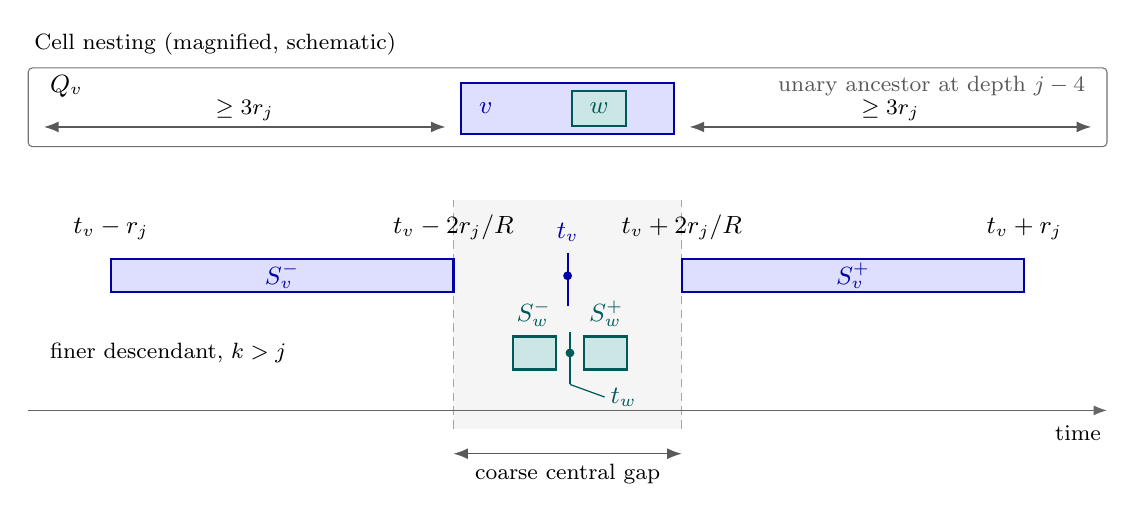
\begin{tikzpicture}[
  x=1cm,y=1cm,
  font=\small,
  >=Latex,
  coarse/.style={draw=blue!65!black,fill=blue!13,line width=.8pt},
  finer/.style={draw=teal!70!black,fill=teal!20,line width=.8pt},
  guide/.style={draw=black!35,densely dashed,line width=.45pt},
  dimension/.style={<->,draw=black!65,line width=.5pt},
  every node/.style={inner sep=2pt}
]
\node[anchor=west,font=\footnotesize] at (.35,4.18)
  {Cell nesting (magnified, schematic)};
\draw[draw=black!55,rounded corners=1.5pt] (.35,2.88) rectangle (14.05,3.88);
\node[anchor=west] at (.55,3.65) {$Q_v$};
\node[anchor=east,font=\footnotesize,text=black!65] at (13.85,3.65)
  {unary ancestor at depth $j-4$};
\draw[coarse] (5.85,3.04) rectangle (8.55,3.69);
\node[anchor=west,text=blue!65!black] at (6.0,3.37) {$v$};
\draw[finer] (7.26,3.14) rectangle (7.94,3.59);
\node[text=teal!70!black] at (7.60,3.37) {$w$};
\draw[dimension] (.55,3.13) -- (5.65,3.13)
  node[midway,above,font=\footnotesize] {$\ge 3r_j$};
\draw[dimension] (8.75,3.13) -- (13.85,3.13)
  node[midway,above,font=\footnotesize] {$\ge 3r_j$};

\fill[black!4] (5.75,-.70) rectangle (8.65,2.20);
\draw[guide] (5.75,-.70) -- (5.75,2.20);
\draw[guide] (8.65,-.70) -- (8.65,2.20);
\draw[->,draw=black!60] (.35,-.47) -- (14.05,-.47);
\node[anchor=east,font=\footnotesize] at (14.05,-.76) {time};

\draw[coarse] (1.4,1.03) rectangle (5.75,1.45);
\draw[coarse] (8.65,1.03) rectangle (13.0,1.45);
\node[text=blue!65!black] at (3.575,1.24) {$S_v^-$};
\node[text=blue!65!black] at (10.825,1.24) {$S_v^+$};
\node[anchor=south] at (1.4,1.62) {$t_v-r_j$};
\node[anchor=south] at (5.75,1.62) {$t_v-2r_j/R$};
\node[anchor=south] at (8.65,1.62) {$t_v+2r_j/R$};
\node[anchor=south] at (13.0,1.62) {$t_v+r_j$};
\draw[draw=blue!65!black,line width=.65pt] (7.20,.85) -- (7.20,1.53);
\fill[blue!65!black] (7.20,1.24) circle (1.6pt);
\node[anchor=south,text=blue!65!black] at (7.20,1.60) {$t_v$};

\draw[finer] (6.505,.05) rectangle (7.04875,.47);
\draw[finer] (7.41125,.05) rectangle (7.955,.47);
\node[anchor=south,text=teal!70!black] at (6.77,.52) {$S_w^-$};
\node[anchor=south,text=teal!70!black] at (7.69,.52) {$S_w^+$};
\draw[draw=teal!70!black,line width=.65pt] (7.23,-.14) -- (7.23,.53);
\fill[teal!70!black] (7.23,.26) circle (1.6pt);
\draw[draw=teal!70!black,line width=.45pt] (7.23,-.14) -- (7.67,-.30);
\node[anchor=west,text=teal!70!black] at (7.67,-.30) {$t_w$};
\node[anchor=west,font=\footnotesize] at (.55,.26)
  {finer descendant, $k>j$};
\draw[dimension] (5.75,-1.02) -- (8.65,-1.02);
\node[anchor=north,font=\footnotesize] at (7.20,-1.08)
  {coarse central gap};
\end{tikzpicture}
\caption[Disjoint regular sampling slots]{%
Regular sampling slots from Lemma~\ref{arm:regular-slots}.
The inset shows cell containment; the two slot rows share one time axis
and are vertically separated for visibility.  Here $r_j=R^2\delta_j$,
the unary ancestor $Q_v$ lies at depth $j-4$, $v$ is its sole occupied
depth-$j$ descendant, and $\operatorname{dist}(v,\partial Q_v)\ge3r_j$.
For a finer descendant $w\subset v$ at depth $k>j$,
$|t_w-t_v|+r_k\le\delta_j+r_j/R
=r_j(R^{-2}+R^{-1})<2r_j/R$;
thus both finer slots lie strictly inside the coarse central gap,
although they need not lie inside the cell $v$.
For an incomparable retained node at depth $k\ge j$,
$|t_w-t_v|\ge3r_j>r_j+r_k$.
These inequalities give disjointness in both cases.}
\label{fig:regular-slots}
\end{figure}


\begin{remark}[Other fixed test bands]\label{arm:other-test-bands}
The same construction applies to a fixed finite family of test bands
contained in $a_*r\leq |t-t_v|\leq A_*r$, where
$0<a_*<A_*<\infty$.  First refine the location boxes until their width
is at most $a_*r/4$, and sample generations far enough apart that the
next outer radius is at most $a_*r/4$.  This uses a fixed larger grid
ratio or a fixed residue class of generations; an independent uniform
choice of the residue preserves uniform sampling of levels.  Increase
the boundary padding beyond $2A_*r$ and then increase the fixed ancestor
depth $g$ if necessary.  A finer descendant's bands are now inside the
coarser inner gap, while an incomparable descendant lies outside the
padded ancestor.  The preceding disjointness proof applies verbatim to
these two explicit inequalities.  The structural and boundary counts
have the same form, with constants depending on the fixed bands.
For integer word times, rounding slot boundaries inward preserves
disjointness and changes normalized lengths by a vanishing amount.
\end{remark}

\begin{lemma}[Integrated connectivity errors]\label{arm:jump-errors}
For each fixed $K,R$, a jump entry at terminal level $\ell$ contributes
at most $C_{K,R}<\infty$ to the expected sum of its separated coarse
projections.  Consequently, if $M_{\mathrm{jump}}$ is the number of jump
entries,
\begin{equation}\label{arm:jump-sum}
 \mathbb E_U\sum_{j=0}^JD_j
 \leq C_{K,R}M_{\mathrm{jump}}.
\end{equation}
If the bases lie in an interval of length at most $C H e^{-N}$ and
$j_N=\lfloor N/\lambda\rfloor$, then also
\begin{equation}\label{arm:base-merger-error}
 \mathbb E_U\sum_{j=0}^{j_N}(b_j-1)\leq C'_{C,R}.
\end{equation}
For a sparse family with $P=O(N/L)$ probes, $L\longrightarrow\infty$,
and fixed list bound $K$, there is a deterministic $d_N=o(N)$ such that,
uniformly in the selected witness data,
\begin{equation}\label{arm:good-connectivity}
 \mathbb P_U\left\{
 \sum_{j=0}^JD_j+
 \sum_{j=0}^{j_N}(b_j-1)>d_N\right\}=o(1).
\end{equation}
Moreover $C_RM=o(N)$.  Together with
Lemma~\ref{arm:regular-slots}, these assertions hold simultaneously on
a set of displacements of conditional probability at least $1/2$ for
all sufficiently large $N$.
\end{lemma}
\begin{proof}
Two fixed times at distance $d$ lie in different uniformly displaced
cells of width $\delta_j$ with probability at most
$\min\{1,d/\delta_j\}$.  Therefore a jump of length at most
$K\delta_\ell$ has expected total separated projections at most
\[
 \sum_{j=0}^\ell\min\{1,K R^{j-\ell}\}
 \leq \sum_{a=0}^\infty\min\{1,K R^{-a}\}
 =:C_{K,R}<\infty.
\]
Linearity proves Equation~\eqref{arm:jump-sum}.  For
Equation~\eqref{arm:base-merger-error}, list the bases in increasing
order and join consecutive bases by artificial edges for counting only.
At every depth, $b_j-1$ is bounded by the number of these edges that
cross a cell boundary.  Their total Euclidean length is at most
$CHe^{-N}$.  Hence
\[
 \mathbb E_U(b_j-1)\leq C e^{-N}R^j,
 \qquad
 \sum_{j=0}^{j_N}C e^{-N}R^j\leq \frac{CR}{R-1}.
\]
For fixed $K$, both $M$ and $M_{\mathrm{jump}}$ are bounded by a fixed
multiple of $P+h_0$.  Choose $d_N=o(N)$ so slowly that
$(P+h_0+1)/d_N\longrightarrow0$.  Markov's inequality gives
Equation~\eqref{arm:good-connectivity}; the bound $C_RM=o(N)$ follows
from $P=o(N)$.  The last assertion follows by intersecting this event
with the event of Lemma~\ref{arm:regular-slots}.
\end{proof}

\begin{lemma}[Stability under an independent grid displacement]
\label{arm:grid-partition-stability}
Fix a marker system with $M$ entries before sampling its displacement.
At level $j$, partition its active entries without using a grid: first
group entries at the same time, then join consecutive distinct active
positions whenever their gap is strictly less than $\delta_j$.
Denote the resulting partition by $\mathcal P_j^*$, and let
$\mathcal P_j(U)$ be the partition into occupied cells of the displaced
grid.  Put
\[
 \Delta(U)=\#\{0\le j\le J:\mathcal P_j(U)\ne\mathcal P_j^*\}.
\]
For an independent uniform displacement,
\begin{equation}\label{arm:grid-partition-error}
 \mathbb E_U[\Delta(U)\mid\text{marker system}]
 \le \frac{2R}{R-1}M.
\end{equation}
At every level where the partitions agree, the entire projected
colored graph, including its base labels, is the same up to cell names.
In particular, if $M\le M_N=o(N)$, two independent uniform
displacements give the same projected graphs outside $o(N)$ levels
with probability tending to one, uniformly over the selected marker
system.
\end{lemma}

\begin{proof}
If $M=0$, all partitions are empty and the assertions are immediate.
Keep the labels and incidences of coincident entries when grouping
their positions.  As $j$ increases, entries and hence distinct active
positions can only disappear.  Initially there are at most $M-1$
consecutive-position pairs; deleting one position creates at most one
new pair.  Thus at most $2M-1$ distinct consecutive pairs occur over
all levels.  Deleting all positions with a common terminal level one
at a time only enlarges this bound.

Every grid partition refines $\mathcal P_j^*$: positions in the same
half-open cell have total span strictly less than $\delta_j$, and so
do all their successive gaps.  The partitions can differ only if a
consecutive active pair with gap $d<\delta_j$ is split by a cell
boundary.  For a fixed pair this has probability $d/\delta_j$, since
$U$ modulo $\delta_j$ is uniform.  For each positive gap,
\[
 \sum_{j:\,\delta_j>d}\frac d{\delta_j}
 \le \frac R{R-1}.
\]
The same bound holds after restricting to the levels at which the
pair is consecutive and active.  A union bound over pairs and levels
proves Equation~\eqref{arm:grid-partition-error}.

All active edge incidences and base labels were fixed before the grid,
so equal marker partitions give identical projected graph data.
Choose a deterministic $q_N=o(N)$ with $M_N/q_N\to0$.
Markov's inequality bounds the conditional probability of
$\Delta(U)>q_N$ by $2RM_N/((R-1)q_N)=o(1)$.  Apply this to each of
two independent displacements.  Outside that exceptional event they
both agree with $\mathcal P_j^*$ except at at most $2q_N$ levels.
The estimate is conditional on arbitrary marker data, so it also
holds under any selection law sampled before the displacements.
\end{proof}

\begin{remark}[Why the order of selection matters]
The witnesses in Definition~\ref{arm:address-forest} must precede $U$.
For example, take two terminal positions $U-\eta$ and $U+\eta$ with
$\eta\ll\delta_J$.  They occupy distinct unary branches on opposite
sides of the persistent boundary $U$ at all $J+1$ levels, but the
same-level paired slots overlap.  At least half the $2(J+1)$ nodes
must be deleted, although there are only two terminal entries.  This
contradicts a bound $C_RM+\varepsilon T$ with $\varepsilon<1/2$ for
large $J$.  Our conditional estimates avoid this obstruction.  We keep
$U$ independent in the probability argument, rather than treating a
sample-dependent favorable displacement as free fixed information.
\end{remark}

\Needspace{8\baselineskip}
\subsection{Counting the address codes}

\begin{lemma}[Address code count]\label{arm:address-codes}
Fix $U$ and the distinct probe depths $j_1,\ldots,j_P$.  Include the
base entries in the probe list at depth $J$, adding that depth if needed,
and enlarge $K$ to cover those entries.  The resulting probe depths
remain distinct.  Suppose each list has at most $K$ marker and edge entries.  There is a coding of the
projected forests and their list incidences with the following bound,
uniformly in the total occupancy $T$:
\begin{align}
 \log\#\{\text{codes of occupancy }T\}
 &\leq(\lambda+C_0)T
   +KP\log(1+T/P)
   +CPK\log(K+1)+O(1).\label{arm:address-code-count}
\end{align}
The constant $C_0$ does not depend on $K$.  A family of additional
annotations with at most $C_a^{m_j}$ choices at depth $j$, for a fixed
$C_a$, only increases $C_0$ by $\log C_a$.
In particular, for fixed $K$ and $P=o(N)$,
\begin{equation}\label{arm:address-code-leading}
 \log\#\{\text{codes of occupancy }T\}
 \leq(\lambda+C_0)T+o(T+N),
\end{equation}
uniformly in $T$.  A sufficient condition for a growing bound $K=K_N$
and probe stride $L$ is
\begin{equation}\label{arm:growing-list-condition}
 \frac{K_N\log(K_NL)}{L}\longrightarrow0.
\end{equation}
The codes can also be assigned subprobability weights at an additional
cost $2\log(T+1)+O(1)$.
\end{lemma}
\begin{proof}
An ordered forest with $T$ vertices and at most two roots has at most
$C4^T$ possible shapes.  One way to see this is to attach a new root
above its roots and use the depth-first parenthesis word of the
resulting ordered tree; its length is $2(T+1)$, and a balanced
parenthesis word determines the tree.  Each nonroot cell has one of
$R$ child offsets in its parent, so the shape has at most $R^T$
geometric assignments.  The occupied root cells have a bounded presence
mask among the cells meeting $I$, whose names are already fixed by
$I,U$.  This proves the bound $C(4R)^T$ for the forest before labels.
Its vertices' depths follow from its parent relation.

At probe depth $j_p$, name a position by its ordered index among the
$m_{j_p}$ occupied cells; use one extra index for an absent list entry.
Thus the position entries have at most $(1+m_{j_p})^K$ possibilities.
Repeated indices record coincident positions.  Names in different
probe lists do not require global forest indices: each local index
specifies a forest vertex, whose ancestors are already determined by
the forest.  A correspondence to a distinguished base uses that base's
fixed name, and its depth-$J$ address determines its coarser addresses.
The list's chain order, colors, endpoint incidences, and base names have
at most $\exp(CK\log(K+1))$ possibilities.  The count includes absent
entries and shorter lists.  It never specifies an exact endpoint
within its terminal cell.

Multiply these choices and use the distinctness of probe depths to
obtain $\sum_p m_{j_p}\leq T$.  Concavity gives
\[
 \sum_{p=1}^P\log(1+m_{j_p})
 \leq P\log(1+T/P),
\]
which proves Equation~\eqref{arm:address-code-count}.  The same estimate
bounds the maximum number of list decorations over all forest shapes,
so variation of the individual $m_j$ between shapes causes no extra
factor.

For $0<\eta\leq K$ and $z\geq0$,
\[
 K\log(1+z)\leq\eta z+K\log(K/\eta).
\]
Indeed the maximum of $\log(1+z)-(\eta/K)z$ occurs at
$z=K/\eta-1$ and is at most $\log(K/\eta)$.  Hence
\begin{equation}\label{arm:address-code-formbound}
 \log\#\{\text{codes of occupancy }T\}
 \leq(\lambda+C_0+\eta)T
   +KP\log(K/\eta)+CPK\log(K+1)+O(1).
\end{equation}
For fixed $K$, let $\eta$ tend to zero sufficiently slowly while
$P=o(N)$.  This yields Equation~\eqref{arm:address-code-leading}
uniformly in $T$.  Under Equation~\eqref{arm:growing-list-condition},
for example $\eta_N=1/\log L$ for large $L$ makes both remainders in
Equation~\eqref{arm:address-code-formbound} equal to $o(N)$.
No condition $L\gg\log N$ is used.  If the probe depths themselves
must be encoded among the $J+1$ levels, their extra cost is at most
$\log\binom{J+1}{P}\leq P\log(e(J+1)/P)=o(N)$ for
$P=O(N/L)$; alternatively their independent mesh displacement can be
conditioned on.

Finally give $T$ a weight proportional to $(T+1)^{-2}$ and distribute
that weight uniformly among its finite enumeration of codes.  The
weights sum to at most one, and the negative logarithm of each weight
is the code count bound plus $2\log(T+1)+O(1)$.
\end{proof}

We call a displacement \emph{favorable} if it satisfies the boundary
bound of Lemma~\ref{arm:regular-slots} and the connectivity bound of
Lemma~\ref{arm:jump-errors}.  For fixed $R,K$, its conditional
probability given the selected witness system is at least $1/2$ for
large $N$.  At a favorable displacement the structural deletions are
$o(N)$ and
\begin{equation}\label{arm:total-rank-lower}
 E:=\sum_{j=0}^Je_j
 \geq T-h_0(J+1)-d_N.
\end{equation}
For earlier scales, Equation~\eqref{arm:base-merger-error} also gives
the stronger replacement of $h_0$ by one, up to an integrated $o(N)$
error.  The simpler bound in Equation~\eqref{arm:total-rank-lower}
suffices for the following occupancy estimate.


The code now specifies every box, component, and sampling slot.  It remains
to bound the probability that its required contacts occur.  We first
control the sum of contour oscillations across its prescribed intervals.

\subsection{Oscillations and the probability of a fixed code}

\begin{lemma}[An exponential sum bound for prescribed intervals]
\label{arm:oscillation-sum}
Consider a deterministic finite family $\mathcal I$ of intervals whose
lengths belong to a geometric family with ratio $R>1$.  Suppose that
at each length at most $K$ intervals cover a point.  There are constants
$c,C>0$, depending on $R,K$ and the raw-word law, such that
\[
 \mathbb P\left\{
  \sum_{I\in\mathcal I}\frac{\operatorname{osc}_I Z}{\sqrt{|I|}}
       >u|\mathcal I|\right\}
 \le \exp\{-cu|\mathcal I|+C|\mathcal I|\}.
\]
Here coordinate oscillations can be summed, and the estimate holds for
all exterior typings.  Integer intervals of bounded length can be
handled by increasing the constant.  If $K$ is fixed and $R\ge2$, the
constants can be chosen uniformly in $R$.
\end{lemma}

\begin{proof}
Cut the union of the intervals at all their endpoints.  There are at
most $2|\mathcal I|$ nonempty atoms $J$.  Proposition~\ref{arm:raw-exponential}
gives independent dominating variables
$Y_J=2M_{|J|}/\sqrt{|J|}$, with a common exponential-moment bound, for
the oscillations on these disjoint fresh raw pieces.  Subadditivity
of oscillation gives
\[
 \sum_{I\in\mathcal I}\frac{\operatorname{osc}_I Z}{\sqrt{|I|}}
 \le\sum_J a_JY_J,
 \qquad
 a_J=\sqrt{|J|}\sum_{I\supset J}|I|^{-1/2}.
\]
If $I_0$ is the shortest interval containing $J$, then
\[
 a_J\le K\sqrt{|J|/|I_0|}
             \sum_{v\ge0}R^{-v/2}
 \le \frac K{1-R^{-1/2}}.
\]
Apply the exponential-moment bound with a parameter divided by this
last constant, and use Markov's inequality.  This proves the claim.
The bound on $a_J$ is uniform for $R\ge2$, proving the asserted
uniformity.
\end{proof}

\begin{proposition}[Fixed-code arm test]\label{arm:fixed-code-test}
Let $\lambda=\log R$.  In the finite shifted address model, fix a code,
let $m_j$ be its number of occupied boxes at level $j$, and let $e_j$
be the sum of its two monochrome ranks.  Put
\[
 T=\sum_jm_j,\qquad E=\sum_je_j,
\]
and let $M$ be the number of terminal entries.  For each $\zeta>0$, one
can choose a fixed sufficiently large $R$ and sufficiently small fixed
deletion tolerances so that, as the minimum sampling radius tends to
infinity,
\begin{equation}\label{arm:fixed-code-probability}
 \mathbb P\{\hbox{the code's chord constraints are realizable}\}
 \le \exp\{-\beta\lambda E+\zeta\lambda T+C_{R,\zeta}M\}.
\end{equation}
The statement is for codes with the regular-slot deletion bound of
Lemma~\ref{arm:regular-slots}.  It is uniform over such finite codes
and over arbitrary exact chord endpoints inside their recorded boxes.
Small fixed errors in sampling radii or inward integer rounding are
absorbed by increasing the minimum permitted radius.
\end{proposition}

\begin{proof}
Choose a deterministic time before all the code's representative
points and sampling slots, and anchor both contour coordinates at
zero there.  A common coordinate translation changes none of the
chord constraints or slot tests.  With this convention the heights
observed while exposing the finite word window are measurable in
its chronological raw filtration, even when the original bilateral
contours had been anchored at time zero inside that window.

For each coordinate and each projected chord component, apply the
sorted comparison lemma to the occupied intervals of that component.
It gives a comparison between consecutive occupied intervals, one per
unit of monochrome rank, with a total height-discrepancy bound of at
most six times the sum of the relevant box oscillations.  A box is
used in at most one component of each color.  Therefore the sum of
all normalized comparison discrepancies is controlled by a fixed
multiple of the normalized box oscillations.

Include also the intervals between each regular-node representative midpoint and
its adjacent sampling-slot endpoint.  Their lengths are comparable
to $r/R$ at a node of sampling radius $r$.  The same-scale overlaps
are bounded independently of $R$: regular centers are separated at
the scale $r$, whereas the box intervals themselves have disjoint
interiors.  Thus Lemma~\ref{arm:oscillation-sum} applies, separately
to a bounded number of geometric length families.  For fixed
$0<\epsilon<\delta$, outside an event of probability at most
\[
 \exp\{-cR^\epsilon T+CT\},
\]
the sum of all these normalized oscillations is at most $R^\epsilon T$.
Discard each comparison whose assigned discrepancy exceeds
$R^\delta\sqrt{r/R}$, and each node-side with an excessive local
oscillation.  At most $C R^{\epsilon-\delta}T$ comparison incidences
are lost.  The originally irregular nodes lose at most
$C\epsilon_0T+C_RM$ incidences: after sorting, a node has at most
one predecessor and one successor per color.  Choosing $R$ large
makes the first two relative losses as small as required.

All remaining required slot conditions now have fixed deterministic
tolerance $C R^\delta\sqrt{r/R}$.  On a left slot the target wall is
the already observed representative height in the previous occupied
box of the same component, minus that tolerance.  The comparison
bound makes survival above this wall and landing near it necessary.
The previous box lies strictly before the slot, by regular-node
separation.  On a right slot use the current midpoint height minus
the same tolerance; that height is already observed before this
slot.  Its initial discrepancy is small by the retained local
oscillation condition.  We do not choose a random wall using the
unobserved actual comparison error.

Expose all slots in chronological order.  Lemma~\ref{arm:regular-slots}
makes them disjoint, and the intervening raw words can also be
exposed in chronological order.  Each slot is fresh conditional on
this history.  If $k$ colors are incident on a retained left slot,
Lemma~\ref{arm:lattice-slots} gives logarithmic charge at least
\[
 (k/2+d_k-O(\delta)-o(1))\lambda.
\]
For a right slot it gives
$(d_k-O(\delta)-o(1))\lambda$.  The $o(1)$ is uniform once the
minimum radius is sufficiently large for the fixed $R$.
Summed incoming incidences give $E/2$ before deletions.  There are
$2E$ side incidences in total, and
$d_k\ge k d_2/2$ for $k=0,1,2$.  The undeleted leading survival
charge is therefore at least $d_2E$.  Deletions lose only a bounded
charge per incidence.  The choices of deleted incidences have at
most $\exp(CT)$ possibilities, which are summed rather than
conditioned upon.

Choose $\delta$ sufficiently small in terms of $\zeta$, then choose
$R$ large enough that $C/\lambda$, the deletion fractions, and the
fixed Brownian constants divided by $\lambda$ fit within the
remaining error budget.  The oscillation-exception exponent can
simultaneously be made larger than $3\beta\lambda T$ in absolute
value, since $R^\epsilon/\log R\to\infty$.  As $E\le2T$, that
exception is absorbed into Equation~\eqref{arm:fixed-code-probability}
after an arbitrarily small enlargement of its error budget.  Finally
take the minimum radius large enough for the uniform lattice-slot
estimates.  Chronological multiplication and the finite sum over
discard patterns give the proposition.
\end{proof}


\subsection{The address occupancy bound}

The fixed-code probability bound outweighs the address count because
$\beta>1$.  We combine them before returning to the independent grid,
so a favorable displacement is never treated as uncharged selected data.

\begin{proposition}[Exponential occupancy bound]\label{arm:occupancy-tail}
Put $\beta=1/2+d_2>1$.  Assume the fixed-code test of
Proposition~\ref{arm:fixed-code-test} in the following quantitative form:
for every sufficiently small $\zeta>0$, choose a fixed boundary
tolerance sufficiently small and a fixed $R$ sufficiently large so
that, once the minimum radius is sufficiently large, every
\emph{favorable admissible} decorated code $\mathfrak c$ satisfies
\begin{equation}\label{arm:required-fixed-code-bound}
 \mathbb P\{\mathfrak c\text{ is realized}\}
 \leq\exp\bigl\{-\beta\lambda E(\mathfrak c)
          +\zeta\lambda T(\mathfrak c)
          +C_{R,\zeta}M(\mathfrak c)\bigr\}.
\end{equation}
This estimate is required uniformly in the fixed displacement $U$.
The realization event includes all the actual marked chord constraints.
The fractional boundary deletions are absorbed into the $\zeta\lambda T$
term, and the structural deletions into the explicit terminal term,
using the bounded number of sorted-chain charges at each deleted
vertex.  The fixed-code estimate includes its oscillation exceptions.
No such estimate is asserted here for codes whose slots are
predominantly irregular.

Then there are $C,c,C_1>0$, independent of any fixed finite exploration
cutoff, such that for all sufficiently large $N$ and all $u\geq0$,
\begin{equation}\label{arm:occupancy-exponential-tail}
 \mathbb P\{A\geq CN+u\}
 \leq C_1\exp(-cN-cu).
\end{equation}
The estimate holds for any word-dependent selection of witness lists
made before $U$.  It also holds for a fixed reference grid, and with
$A$ replaced by its maximum over grid displacements.  The threshold
in ``sufficiently large'' may depend on the fixed exploration cutoff.
If Equation~\eqref{arm:address-tilt} holds, then
\begin{equation}\label{arm:occupancy-tilted-mean}
 \mathbb E_{\mathbb Q_N}A=O(N).
\end{equation}
The corresponding code has length at most a deterministic constant
times $N$ with $\mathbb Q_N$-probability tending to one.  At an
independently and uniformly sampled level $j\in\{0,\ldots,J\}$,
$\mathbb E_{\mathbb Q_N}m_j=O(1)$.
\end{proposition}
\begin{proof}
Fix $U$.  Use Equation~\eqref{arm:address-code-formbound} with a small
fixed $\eta>0$ and then let the sparse terminal error be $o(N)$.
For every favorable code of total occupancy $T$, combine
Equations~\eqref{arm:required-fixed-code-bound} and
\eqref{arm:total-rank-lower}.  Summing over its possible codes gives
\begin{align*}
 &\mathbb P\{\text{some favorable realized code has occupancy }T\}\\
 &\quad\leq
 \exp\bigl\{
 -[(\beta-1-\zeta)\lambda-C_0-\eta]T
 +\beta\lambda h_0(J+1)
 +\beta\lambda d_N+C_{R,\zeta}M+o(N)
 \bigr\}.
\end{align*}
Choose fixed $R$ large enough and then the error tolerances small enough
that
\[
 \delta:=\beta-1-\zeta-(C_0+\eta)/\lambda>0.
\]
Since $\lambda(J+1)=bN+O(1)$, $d_N=o(N)$, and $M=o(N)$, there is a fixed
$B<\infty$ such that the last probability is at most
\begin{equation}\label{arm:fixed-occupancy-union}
 \exp\{-\delta\lambda T+BN\}.
\end{equation}
Here $B$ and $\delta$ are independent of the fixed list cutoff: its
contribution was confined to the sparse $o(N)$ terms.  Geometric summation
over $\lambda T\geq x$ shows, uniformly in $U$,
\[
 \mathbb P\{\text{favorable and }A\geq x\}
 \leq C_2\exp(BN-\delta x).
\]
For $C_*=(B+2)/\delta$, this gives
\begin{equation}\label{arm:favorable-tail}
 \mathbb P\{\text{favorable and }A\geq C_*N+u\}
 \leq C_2\exp(-2N-\delta u).
\end{equation}
The same bound holds after integrating over the independent $U$.

The event of a favorable displacement has only a positive conditional
probability; we do not give its complement an exponential estimate.
Instead compare all shifts of the same realized witness system.  The
same-width cell intersection argument gives
\[
 T(U)\leq2T(V)\qquad\text{for all displacements }U,V.
\]
Let $A_{\max}=\max_U\lambda T(U)$.  This maximum is measurable:
there are finitely many markers and levels, so only finitely many
marker--boundary crossings can change the occupancy as $U$ varies in
$[0,H)$.  If $A_{\max}\geq x$, every displacement has $A\geq x/2$,
and at least half of the displacements are favorable.  Conditional on
the complete witness system, this proves
\[
 \mathbf 1_{\{A_{\max}\geq x\}}
 \leq2\mathbb P_U\{\text{favorable and }A\geq x/2
                      \mid\text{witness system}\}.
\]
Integrate and apply Equation~\eqref{arm:favorable-tail}.  Increasing
the constant multiplying $N$ proves
Equation~\eqref{arm:occupancy-exponential-tail} for $A_{\max}$, and
therefore for every particular grid.  All word-dependent choices have
been included in the finite code enumeration.  The auxiliary favorable
shift has never been selected as unencoded sample-dependent information.

Under Equation~\eqref{arm:address-tilt}, the tail is bounded above by
\[
 \mathbb Q_N\{A\geq CN+u\}
 \leq\min\{1,C_1\exp(k_N-cN-cu)\}.
\]
Since $k_N=o(N)$, integration in $u$ gives
\[
 \mathbb E_{\mathbb Q_N}A
 \leq CN+C_1c^{-1}\exp(k_N-cN)=O(N).
\]
Equation~\eqref{arm:address-code-formbound}, including its optional
integer-size code, then gives the stated deterministic $O(N)$ code
cutoff outside an event of probability tending to zero.  Finally,
for an independently uniform level,
\[
 \mathbb E_{\mathbb Q_N}m_j
 =\frac{\mathbb E_{\mathbb Q_N}T}{J+1}=O(1),
\]
since $J+1$ is comparable to $N$ for fixed $R,b$.
\end{proof}

\begin{remark}[Finite cutoffs and the order of limits]
Fix the desired error tolerance first, then choose $R$ and the padding
constants.  For each fixed finite exploration bound, let $N$ and the
minimum time unit diverge, and let the probe stride satisfy
$L\longrightarrow\infty$ and $L=o(N)$.  Structural, jump, and terminal
code errors are then $o(N)$.  A subsequent slow diagonal may increase
the exploration and list bounds, retaining
Equation~\eqref{arm:growing-list-condition} and the vanishing jump
error.  For example, the constant in Equation~\eqref{arm:jump-sum}
is $O(1+\log_R K)$, so that the displayed growing-list condition also
controls that error when the jump tolerance is bounded by $K_N$.
The coefficient in the occupancy bound remains fixed; only the speed
of the diagonal changes.  The construction counts all projected
addresses, including intermediate markers from different probe levels.
It assumes no sparsity of the original candidate locations at a finest
scale.  Producing a saturated, jointly realizable finite-line system
from the occupancy bound is a separate step.
\end{remark}
\subsection{The credit contradiction and entropy of viewed blocks}

For a connected component $C$ of a union of two colored graphs, let
$e(C)$ be the sum of the ranks of the two colored graphs restricted to
$C$, where rank is the number of vertices minus the number of connected
components, including isolated vertices.  We say that $C$ has a
\emph{rank cycle} when $e(C)\ge |C|$, and that it is \emph{acyclic}
when $e(C)=|C|-1$.  The union spanning-tree argument in
Lemma~\ref{arm:projected-rank} shows that these alternatives exhaust the
possibilities.  Thus an acyclic component has exactly the minimum total
rank needed for connectivity.

\begin{proposition}[Rank credit]\label{arm:rank-credit}
Let $\varepsilon=\beta-1>0$.  Consider the projected witness systems
of the address construction on logarithmic levels $[0,bN]$, with
$h$ bases in an interval of length $O(ne^{-N})$.  Suppose their
pairwise time distances exceed the largest address-cell width used
on $[aN,bN]$, where $1<a<b$; thus they occupy distinct boxes there
for every displacement.  All selected
laws satisfy $\mathbb Q_N\le e^{o(N)}\mathbb P$.  Then the following
combination of events has probability tending to zero: outside a
vanishing fraction of levels in $[aN,bN]$, every connected
component containing a base has a rank cycle.

Here $a-1$ is chosen sufficiently small relative to
$\varepsilon(b-a)$, and then $h$ sufficiently large, with all choices
fixed before the scaling limit.  Witness-list cutoffs may increase
only along the sparse diagonals allowed by the address construction.
\end{proposition}

\begin{proof}
At a level with $m$ occupied boxes, $c$ union components, and total
monochrome rank $e$, one has
\[
 e\ge m-c,\qquad m-\beta e\le\beta c-\varepsilon m.
\]
The integrated component excess caused by projected jumps is $o(N)$
on favorable grids.  Before level $N$, all base cells can be charged
as one component up to $o(N)$; hence the possible positive credit
there is at most $C_0N+o(N)$, independently of $h$.  On $[N,aN]$,
there are at most $h$ base components, so positive credit is at most
$C_1(a-1)hN+o(N)$.  The constants include fixed endpoint-rounding
and grid-step changes.

At every level on which all base components have rank cycles,
$e\ge m$ after the negligible connectivity errors.  The separated
bases occupy at least $h$ boxes on $[aN,bN]$, so the credit there is
at most $-\varepsilon h$ per unit log length.  At exceptional levels
the positive credit can still be bounded by a constant times the
number of acyclic base components; a bound on the maximum $m$ is
not needed.  Proposition~\ref{arm:occupancy-tail} absorbs all small
relative errors in the integrated occupancy into an arbitrarily
small multiple of $N$.

Choose $a-1$ such that
$C_1(a-1)<\varepsilon(b-a)/4$, and then choose $h$ with
$C_0<\varepsilon(b-a)h/4$.  The total leading address budget minus
arm charge is then at most $-cN$ for some $c>0$, even after the
permitted errors.  Summing Equation~\eqref{arm:fixed-code-probability}
over the length-weighted codes gives an exponentially small
probability for the stated cycle event \emph{and a favorable
displacement}, under $\mathbb P$.  Multiplying by $e^{o(N)}$ gives
the same vanishing conclusion under $\mathbb Q_N$.

We now remove favorability without assuming that cyclicity is
invariant under a change of grid.  Let $\eta_N\downarrow0$ and denote
by $E_N(U)$ the cycle event with at most $\eta_NN$ exceptional
generations for the independent displacement $U$.  Generation count
and logarithmic length differ by the fixed factor $\lambda$.
Lemma~\ref{arm:grid-partition-stability} supplies $q_N=o(N)$ and a
uniform conditional error $\alpha_N=o(1)$ such that
$\Delta(U)\le q_N$ outside that error.  Let $E_N^*$ be the corresponding
cycle event for the grid-independent partitions $\mathcal P_j^*$,
with at most $\eta_NN+q_N$ exceptions.  Then
\[
 \mathbb Q_N(E_N(U))\le\mathbb Q_N(E_N^*)+\alpha_N.
\]
Sample a second independent displacement $V$.  Conditional on the
marker system, $V$ is favorable and has $\Delta(V)\le q_N$ with
probability at least $1/2-\alpha_N$.  On $E_N^*$ this gives the
projected cycle event $E_N'(V)$ with at most $\eta_NN+2q_N=o(N)$
exceptional generations.  Consequently
\[
 (1/2-\alpha_N)\mathbb Q_N(E_N^*)
 \le \mathbb Q_N(E_N'(V)\cap\{V\text{ favorable}\}).
\]
The preceding favorable-grid estimate applies to this right side.
Indeed, on each added exceptional level the positive credit is at
most $\beta(h+D_j)$, by Equation~\eqref{arm:rank-component-bound};
the extra levels and the favorable-grid sum $\sum_jD_j$ are both
$o(N)$.  No maximum-occupancy bound is needed for this error.  The
right side therefore tends to zero, proving the claim for $U$.
The conditional grid estimates are uniform in the preselected data;
their errors are not multiplied by the selected density.
\end{proof}

\begin{lemma}[Entropy allocation for a finite address code]
\label{arm:entropy-allocation}
Let $W$ have a product raw-word law $\mathbb P$, including an
independent past if needed.  Let $\mathbb Q\le e^\kappa\mathbb P$,
and let $C$ be a countably valued code chosen using $W$ and independent
auxiliary randomness.  Suppose $C$ has code lengths $\ell(c)$ with
$\sum_c e^{-\ell(c)}\le1$.  For each fixed code, let finitely many
disjoint deterministic word slots be ordered chronologically.  Then
the sum of their expected conditional relative entropies with respect
to fresh iid raw blocks, averaged over $C$, is at most
\begin{equation}\label{arm:entropy-total}
 \kappa+\mathbb E_{\mathbb Q}\ell(C).
\end{equation}
Auxiliary continuous grid shifts can be kept as independent side
information and integrated; no code length for such an independent
shift is charged.
\end{lemma}

\begin{proof}
Let $\pi_c=e^{-\ell(c)}$ and place any missing mass at an unused code.
Compare the joint law of $(C,W)$ under $\mathbb Q$ to the law in
which $C$ has probabilities $\pi_c$ and $W$ independently has law
$\mathbb P$.  The chain rule gives
\[
 D(\mathbb Q_{C,W}\Vert\pi\otimes\mathbb P)
 =D(\mathbb Q_W\Vert\mathbb P)
   +\mathbb E_{\mathbb Q_W}
        D(\mathbb Q_{C\mid W}\Vert\pi)
 \le\kappa+\mathbb E_{\mathbb Q}\ell(C),
\]
because the conditional Shannon entropy of $C$ is nonnegative.
Disintegrate instead first over $C$ and then over the chronological
raw pieces.  Product structure under the reference law makes the
reference conditional law in every slot a fresh iid block.  Discarding
the nonnegative entropy terms for the gaps, past, and other pieces
leaves the asserted upper bound for the slots.  This proof also
applies to finite restrictions of an infinite past, followed by
monotone increase of the observed sigma fields.

For an independent grid displacement $U$, apply the argument
conditionally on $U$ and integrate.  The original word law is
independent of $U$, and the selected law before grid sampling has
the same bounded-density property.  We do not condition on a
sample-dependent favorable displacement before this calculation.
\end{proof}

\begin{corollary}[Central oscillations at intermediate levels]
\label{arm:central-oscillations}
For a projected address code, assign to every occupied node $v$ an
interval of length at most $A r_v$ centered within its location cell,
where $A$ is fixed and $r_v$ is its viewing radius.  Centers rounded
using the terminal address are also allowed, provided they lie in the
specified cell.  Write
\[
 S_v=\frac{\operatorname{osc}_{I_v}Z}{\sqrt{r_v}}.
\]
Suppose $\mathbb E_{\mathbb Q}\sum_jm_j=O(N)$, the expected code length
is $O(N)$, and the selected density bound is $e^{O(N)}$.  Then
\[
 \mathbb E_{\mathbb Q}\sum_v S_v=O(N).
\]
In particular, the sum of the central oscillation amplitudes of the
occupied lines has bounded first moment at a uniform intermediate
viewing level.  The constants may depend on the fixed grid ratios,
padding, and $A$, but not on the exploration-list cutoff.
\end{corollary}

\begin{proof}
Replace each $I_v$ by the deterministic interval
\[
 \widehat I_v=
 [\inf v-A r_v/2,\ \sup v+A r_v/2],
\]
where $v$ denotes the code's location cell.  This interval contains
$I_v$ regardless of the chosen in-cell center.  Its length is exactly
$(A+R^{-2})r_v$.  At a fixed level, location cells have common length
$r_v/R^2$, so these enclosures have overlap multiplicity at most
$C_A R^2$.  Across levels their lengths are geometric.  The proof of
Lemma~\ref{arm:oscillation-sum} gives constants $\theta,c>0$ such
that, for every fixed code,
\[
 \mathbb E_{\mathbb P}
 \exp\left\{\theta\sum_v S_v-c\sum_jm_j\right\}\le1.
\]
The same holds under the product reference in which the code has
its Kraft weights and is independent of the raw word.  The entropy
variational inequality and Lemma~\ref{arm:entropy-allocation} imply
\[
 \theta\mathbb E_{\mathbb Q}\sum_vS_v
 \le c\mathbb E_{\mathbb Q}\sum_jm_j+
       \kappa+\mathbb E_{\mathbb Q}\ell(C)=O(N).
\]
Division by the number of intermediate levels proves the last claim.
\end{proof}

\begin{remark}[Arbitrary off-center bands at a coarsened level]
\label{arm:coarsened-bands}
The entropy allocation is not restricted to seed probe levels.  Fix
finitely many bands $a r\le |t-t_v|\le A r$, with $0<a<A<\infty$,
at the intermediate viewing radius $r$.  Refine the location cells
so their length is at most $a r/8$, retain only a residue class of
levels with successive radius ratio greater than $8A/a$, and increase
the ancestor padding in Lemma~\ref{arm:regular-slots}.  The same
ancestor/descendant proof then makes the enlarged test bands pairwise
disjoint: descendants lie in the inner hole, and incomparable nodes
lie outside the padded ancestor.  The residue class is chosen uniformly
and independently, so averaging over it preserves the uniform-level
marginal.  Its spacing is fixed once the finite band request is fixed.

For origins rounded from terminal address cells, slow coarsening makes
the rounding error $o(r)$.  The deterministic enlarged bands therefore
contain every actual requested block, for large enough coarsening.
One applies Lemma~\ref{arm:entropy-allocation} to the enlarged raw
slots and then takes the requested observations as measurable
functions there.  Structural and boundary deletions are bounded by
the same marker and fractional-occupancy errors.  A continuous
logarithmic phase, if used, is integrated as independent reference
side information; equivalently, stationarity under the fixed grid
dilation already suffices for the zero-or-infinite conclusions about
pinned heights and first sign-change times.
\end{remark}

\section{Finite contour views and protected annuli}
\label{view:section}

We now construct cheap circuits around selected discrete vertices.  The
inputs are the address estimates of Section~\ref{arm:section}, the local
passage kernels, and the bilateral crossing comparison.  The output,
Proposition~\ref{view:acyclic-circuit}, applies whenever the contour
contacts seen from a base form an acyclic component.

The proof has three parts.  First, finitely many contour neighborhoods
cover every bounded exploration from the bases at a typical logarithmic
scale.  One code records these neighborhoods at all seed scales; an
independent coarsening with fixed origins then gives stationary limiting
profiles.  Second, their contact classes determine a finite auxiliary
sphere containing an annulus whose incidences agree with the original
map.  Third, the annular crossing tests are expressed entirely in
retained off-center data and transferred from ordinary Brownian
completions.  This last step estimates open-port crossings only; access
from the surrounded vertex is the task of Section~\ref{spike:section}.

\subsection{Probability spaces and entropy transfer}

For an index $j$, let $P_j$ be the law of the entire bilateral raw inventory
word on its countable product space, resolved using its bilateral past.
Entropy calculations below are first made on finite observations and then
extended by increasing those observations.  Auxiliary grid translations and sampling variables
are independent under $P_j$.  Let $N_j\to\infty$, let $n_j$ be the base time
unit, and put $r_j(x)=n_j e^{-x}$.  We only use levels for which
$n_j e^{-bN_j}\to\infty$.  The selected law $Q_j$ satisfies
\begin{equation}\label{view:selection}
 Q_j\ll P_j,\qquad \frac{dQ_j}{dP_j}\le e^{\kappa_j},
 \qquad \kappa_j=o(N_j).
\end{equation}
Conditioning on an event of probability $e^{-o(N_j)}$ has this form.
The bounded-density hypothesis gives the address first-moment estimates
used below.

We will use bilateral recurrence below every fixed scalar height.  Here
is its inventory justification.  Every letter has a finite match almost
surely, by \cite[Proposition~2.2]{SheffieldInventory}.  At a fixed integer
cut the past stack contains infinitely many burgers of each type: if it
contained exactly $k$ of one type with positive probability, the independent
next $k+1$ letters could all be rigid orders of that type, contradicting
finite matching.  The $k$th remaining burger of a given type, counted from
the freshest, has birth baseline $-k$ relative to that coordinate at the
cut.  Its birth realizes this level in the past, and its eventual matched
order realizes it in the future.  Taking all integer cuts and $k$ proves
the asserted recurrence simultaneously, including at selected origins.
Absolute continuity in Equation~\eqref{view:selection} preserves this
probability-one property.

\begin{lemma}[Macroscopic cutoffs before selection]
\label{view:macroscopic-cutoffs}
Fix a compact starting time interval in a bilateral contour coupling,
a sequence $n_j\to\infty$, and deterministic $\rho_j\downarrow0$.
For every $\epsilon>0$ there are deterministic nested intervals
$[-C_dn_j,C_dn_j]$, one for each integer $d\ge1$, and deterministic
$D_j\to\infty$, such that events $\mathcal T_j$ with
$\limsup_jP_j(\mathcal T_j^c)\le2\epsilon$ have these properties
simultaneously for every $d\le D_j$:
\begin{enumerate}[label=(\roman*)]
\item Every exploration from the starting interval with at most $d$
steps, each either a scalar link or a time jump of magnitude at most
$dn_j$, stays in the
corresponding interval $[-C_dn_j,C_dn_j]$.  The statement includes
the endpoints of actual first- and last-return witnesses.
\item If its jumps have magnitude at most $d\rho_jn_j$, all its
projected points lie within $\alpha_j$ of its base, where
$\alpha_j\downarrow0$ is deterministic.
\end{enumerate}
The events and their full arrays of cutoffs are chosen before any
bad-level, bad-base, or bounded-density selection.  They hold for all
seed levels satisfying $r_j(x)\le\rho_j n_j$.  After selection one
may slow the actual exploration cutoff beneath $D_j$, and may slow
it further to accommodate any fixed finite family of composed
explorations.  No new typicality event is intersected after selection.
\end{lemma}

\begin{proof}
First fix $d$.  Start with a bounded macroscopic time interval $I_0$
containing every permitted base.  Enlarge it by $d$ on each side to
allow a time jump of length $dn_j$.  On this enlarged interval the
limiting Brownian coordinates have finite minima.  In each coordinate
choose one time to its left and one to its right at which that
coordinate is below its minimum on the enlarged interval by more
than three.  Such times exist almost surely by scalar Brownian
recurrence.  They need not be the same times for the two coordinates.
Let $I_1$ contain the enlarged interval and all four chosen times.
A scalar partner of a source in the enlarged interval cannot lie
beyond its corresponding lower barrier: the intervening minimum
would then be strictly smaller than the source height.  Repeat this
enlargement and barrier construction $d+1$ times.  It gives an almost
surely finite random interval containing every such chain, uniformly
over all its choices of source, color, and endpoint.

Choose a deterministic $C_d$ large enough that these finitely many
strict barriers lie in $[-C_d,C_d]$ except with probability at most
$\epsilon2^{-d-2}$.  Increase the constants to make them nested.
Compact-uniform contour convergence preserves all the barrier
inequalities with a margin exceeding one for all sufficiently large
$j$ on this event.  A discrete scalar link changes the tested endpoint
level by at most one lattice step, whose normalized size tends to
zero.  Thus the same argument confines the actual discrete chains.
The barriers also confine their last-upcrossing and first-downcrossing
searches whenever these are used to realize such a source chord.
This is simultaneous containment over the continuum of source times,
not a separate probability estimate for each seed.

For (ii), keep $d$ fixed and use its deterministic enclosing interval.
If uniform spatial collapse failed, some subsequence would have a
base and a chain of at most $d$ steps with a projected separation
bounded below.  Pass to a further subsequence on which all their
rescaled times converge in that compact interval, repeating vertices
to keep the chain length fixed.  The endpoints of a time jump have
the same limit because $d\rho_j\to0$.  The endpoints of an actual
scalar link limit to a scalar horizontal pair, by compact-uniform
contour convergence and its endpoint/minimum test.  They have the
same curve image by Theorem~\ref{bg:continuum-inputs}(iii).
Continuity of the curve then makes every successive pair of projected
chain points have the same limiting image, contradicting the claimed
separation.  This compactness argument is uniform over all bases,
all seed levels, and all choices of a bounded chain.  In particular it
uses only $r_j(x)\le\rho_jn_j$, not the number of tested levels.

For each fixed finite collection $d\le k$, the preceding convergence
and barrier events imply their simultaneous conclusions with spatial
error at most $1/k$ and failure at most $\epsilon+o_j(1)$; the sum of
the displayed barrier budgets is less than $\epsilon/2$.  Choose
deterministic thresholds $j_k$ increasing so that for $j\ge j_k$ the
remaining error is at most $\epsilon$, and put $D_j=k$ between
successive thresholds.  Let $\mathcal T_j$ be that finite intersection
and $\alpha_j=1/D_j$.  This defines a master event with the asserted
probability before any subsequent selection.  Additional deterministic
slow-growth requirements on $D_j$ may be imposed by increasing $j_k$.

If a selected law is supported on $\mathcal T_j$, all these assertions
hold under it by support, without transferring a small ordinary
probability through its density bound.  Every later fixed exploration
or composition bound is eventually below $D_j$.  A diagonal chosen
after that law may only decrease this cutoff, retaining each earlier
window $C_d$ separately.  For a prescribed open spatial neighborhood
with a fixed positive margin about the permitted bases, (ii) gives
the required confinement once $\alpha_j$ is below that margin.
\end{proof}

Whenever we apply the address estimates below, the selected laws are
supported on one of these preselection master events for a fixed
compact starting interval, with $\rho_j$ bounding every used time
scale divided by $n_j$.  This is the finite-chain typicality cutoff.
The loss $2\epsilon$ is removed before forming the bad-configuration
contradiction.

\begin{lemma}[Coding and disjoint slots]\label{view:entropy-slots}
Let $C_j$ be a countable code with lengths $\ell_j(c)$ satisfying
$\sum_c e^{-\ell_j(c)}\le1$.  Conditional on a code, suppose there are
$T_j\ge cN_j$ disjoint chronological raw-word slots, their boundaries and
the observations assigned to them being fixed by the code.  Suppose
$E_{Q_j}\ell_j(C_j)\le K N_j$.  Let $I_j$ be uniform among the slots,
independently after all other sampling.  The mean relative entropy of the
conditional law of the selected raw slot, given its preceding observations
and the code, with respect to its iid raw-word law is at most
$(K+o(1))/c$.
\end{lemma}

\begin{proof}
Apply Lemma~\ref{arm:entropy-allocation} to the selected law, the
code $C_j$, and its chronological disjoint slots.  It bounds the sum
of their expected conditional relative entropies by
$\kappa_j+E_{Q_j}\ell_j(C_j)\le\kappa_j+KN_j$.
If only a coarser preceding history is retained, data processing
gives the same bound for that history.  Since $I_j$ is uniform after
sampling and $T_j\ge cN_j$, its mean conditional relative entropy is
at most $(\kappa_j+KN_j)/(cN_j)=(K+o(1))/c$.
No independence of the resolved walk from its past is asserted or used.
\end{proof}

\begin{lemma}[Null-test transfer]\label{view:entropy-null}
If $Q\ll P$ and $D(Q\Vert P)\le H$, then, for an event $E$ with
$0<P(E)<1$,
\begin{equation}\label{view:binary}
 Q(E)\le\frac{H+\log2}{\log(1/P(E))}.
\end{equation}
Consequently uniformly bounded entropy transfers events whose reference
probabilities tend to zero.  The same conclusion holds for averaged
conditional entropies and uniformly vanishing conditional reference
probabilities.
\end{lemma}

\begin{proof}
Data processing to the indicator of $E$ gives
$D(Q\Vert P)\ge q\log(1/p)-\log2$, where $q=Q(E)$ and $p=P(E)$.
For conditional laws apply this inequality to each section and integrate.
\end{proof}

The conclusion is tight absolute continuity, not a bounded likelihood ratio.
For lattice passage observations Proposition~\ref{loc:slot-domination}
supplies the following additional input: after
fixing finitely many compatible guard and flexible-order instructions, the
iid slot experiment must have a subprobability law dominated by a fixed
multiple of a reference experiment with independent raw blocks and smoothly
sampled shifts on the feasible lattice.  If that domination has error
$\eta$, a reference event of probability $u$ has iid-slot probability at most
$Mu+\eta$; Equation~\eqref{view:binary} applies to this bound.  One first lets
$j\to\infty$, then $u\downarrow0$, and finally $\eta\downarrow0$ by exhausting
the guards and compact parameter ranges.  Brownian weak convergence of the
shifts does not supply this lattice domination.

\subsection{Simultaneous packing and finite-line saturation}

The occupation estimate bounds the number of separated contour
neighborhoods visible from the bases.  We need those neighborhoods and
their connecting links to occur in one realization.  The following
packing construction provides this simultaneous choice.

Here all randomness of the selected environment is sampled before the
viewing level.  Let $I_j$ be a deterministic logarithmic interval of length
$T_j\asymp N_j$, and let $Y_j$ be uniform on $I_j$, independently of that
environment.  For $k\ge1$ let $\mathcal R_{j,k}(x)$ be the lattice times
reachable from the bases using at most $k$ links or time jumps, each jump
having magnitude at most $kr_j(x)$.  Recurrence below every fixed scalar
level in both directions makes each lattice scalar class finite, hence
each bounded-depth reachable set is finite.  Enclosing chronological
windows are only cutoffs for coding and are removed; a link search has
no bound on its chronological duration.  These sets increase with $k$
and satisfy
\begin{equation}\label{view:reach-monotonicity}
 y\le x\quad\Longrightarrow\quad
 \mathcal R_{j,k}(x)\subseteq\mathcal R_{j,k}(y).
\end{equation}
All intermediate points of a witness belong to its reachable set.  A
$\ell$-bounded exploration started from $\mathcal R_{j,k}(x)$ stays in
$\mathcal R_{j,g(k,\ell)}(x)$ for some deterministic $g$; for example,
$g(k,\ell)=2(k+\ell+1)$ suffices.  Define
\[
 P_{j,k,H}(x)=\max\{|A|:A\subseteq\mathcal R_{j,k}(x),\quad
 |u-v|>Hr_j(x)\text{ for distinct }u,v\in A\}.
\]

\begin{lemma}[The required consequence of address occupation]
\label{view:occupation-packing}
Suppose the projected-address estimate holds, with a constant $C$
independent of fixed $k$ and $M$, for simultaneous lists formed as follows.
At the levels of an independently translated mesh of stride $L$, choose
at most $M$ terminals in $\mathcal R_{j,k}$ and include their access
witnesses.  Project each list through the preceding coarser cell of length
$L$.  Its active-box count $m_j$ satisfies
\[
 \int_{I_j}m_j(x)\,dx\le(C+o_L(1))T_j
\]
with probability tending to one, or with any prescribed fixed probability
loss which can subsequently be removed.  The projected boxes have diameter
at most $cr_j(x)$, and the marker errors divided by $T_j$ vanish as
$L\to\infty$ for each fixed $k,M$.  Then
\begin{equation}\label{view:packing-bound}
 \sup_{k,M}\ \lim_{H\to\infty}\limsup_{j\to\infty}
 E_{Q_j}\min\{P_{j,k,H}(Y_j),M\}\le C.
\end{equation}
\end{lemma}

\begin{proof}
Choose $L=L(H)\to\infty$ slowly enough that $He^{-L}>2c$.  At each seed
$y$ take a maximal $H$-packing, truncated at $M$.  Throughout its coarser
cell $[y-L,y]$, the chosen terminals remain in different projected boxes,
since the time unit grows by at most $e^L$.  Thus their count contributes
at least $L$ times itself to $\int m_j$, apart from the two end cells.
Averaging the independent mesh translation converts the sum of these
seed counts into the uniform-level integral.  On the exceptional event
bound the truncated packing by $M$, without attempting to bound $m_j$.
Divide by $T_j$, let $j\to\infty$, remove the prescribed probability loss,
and then let $H$ and $L(H)$ tend to infinity.  The end-cell loss is at most
$2ML/T_j$ and vanishes in the first limit.
\end{proof}

\begin{proposition}[Saturated centers and actual colored witnesses]
\label{view:saturation}
Assume Equation~\eqref{view:packing-bound}.  There is a subsequence and
deterministic $H_j,k_j,L_j\to\infty$ such that
$L_j=o(T_j)$ and $L_j=o(\log H_j)$ with the following properties.
Choose a finite set of centers $\mathcal C_j$ at the seed level $Y_j$,
then independently choose $U_j\sim\operatorname{Unif}[0,L_j]$ and put
$X_j=Y_j-U_j$.  The centers have a finite limiting count $K$ with
$E K\le C$, remain mutually divergent in $r_j(X_j)$ units, and have tight
access depths.  At both $V_j=Y_j$ and $V_j=X_j$, for every fixed $k$,
\begin{equation}\label{view:uniform-target-coverage}
 \lim_{A\to\infty}\limsup_{j\to\infty}Q_j\left[
 \sup_{t\in\mathcal R_{j,k}(V_j)}
 \frac{\operatorname{dist}(t,\mathcal C_j)}{r_j(V_j)}>A\right]=0.
\end{equation}
Finite access witnesses and finitely many actual colored edges can be
chosen simultaneously so that their access depths are tight and all
their within-line time offsets collapse after coarsening.  The limiting
colored graph contains every edge which is witnessed by an actual link
at bounded reach and bounded line coordinates at the coarsened level.
\end{proposition}

\begin{proof}
Take a countable joint subsequential limit of all truncated packing
counts for integer $k,H,M$.  On this common product probability space
write $P_{k,H}$ for the extended-integer limits.  Their monotonicities are
preserved.  Set $A_k=\lim_{H\to\infty}P_{k,H}$ and
$A=\lim_{k\to\infty}A_k$.  Equation~\eqref{view:packing-bound}, first
with finite truncations, gives $EA\le C$.  Thus $A$ is finite, and the
increasing integer sequence $A_k$ equals $A$ eventually on each sample.

At a candidate seed level, construct an $H_j$-separated greedy set by
processing $\mathcal R_{j,1},\ldots,\mathcal R_{j,k_j}$ in that order.
Within each stage add points until maximal, using a fixed measurable
ordering of the finite lattice set.  Let $G_{j,k}$ be its size after
stage $k$.  Maximality and the nearest-center assignment imply
\[
 P_{j,k,3H_j}\le G_{j,k}\le P_{j,k,H_j},\qquad k\le k_j.
\]
Choose $H_j$ and $k_j$ sufficiently slowly that
$G_{j,k}\Rightarrow A_k$ for each fixed $k$, while the final count
$K_j=G_{j,k_j}\Rightarrow A$, jointly with the original fixed-cutoff
array.  Explicitly, at stage $d$ choose a finite height cutoff large
enough to approximate the first $d$ limiting counts and their threefold
cutoffs, then choose $j_d$ so their joint laws for $j\ge j_d$ are within
$1/d$ of those limits; let the stage index tend to infinity only through
these thresholds.  A further slow stage choice handles the depth cutoff.
No convergence rate is required.

Let $D_j$ be the largest access depth of a selected center.  The greedy
construction gives $\{D_j>k\}=\{G_{j,k}<K_j\}$.  In the joint integer
limits the two counts are ordered and have marginals $A_k$ and $A$.
Since these marginals approach the same finite law, their probability of
inequality tends to zero.  Thus $D_j$ is tight.

In a further joint limit write $K$ for the limit of $K_j$ and retain the
entire fixed packing array.  On $D_j\le d$ the selected centers are an
$H$-packing in $\mathcal R_{j,d}$ for every fixed $H$ and all large $j$.
Taking $j$, then $H$, then $d$ to infinity shows $K\le A$ almost surely.
Their laws agree, so $K=A$ almost surely.  For fixed $k,d,H$, a point of
$\mathcal R_{j,k}$ at distance exceeding $Hr_j(Y_j)$ from all centers,
on $D_j\le d$, adds one point to their packing.  Therefore
\[
 Q_j[\text{coverage fails at }H]
 \le Q_j[D_j>d]+Q_j[P_{j,\max(k,d),H}(Y_j)\ge K_j+1].
\]
In the joint limit the second probability tends to zero as $H\to\infty$,
because its packing count decreases to $A_{\max(k,d)}\le A=K$.
Let $d\to\infty$.  This proves the seed version of
Equation~\eqref{view:uniform-target-coverage}.

Choose $L_j\to\infty$ with $L_j=o(T_j\wedge\log H_j)$.  The old centers
remain separated by $H_je^{-L_j}\to\infty$ in the new units, and their
access depth stays tight by Equation~\eqref{view:reach-monotonicity}.
Independence of the seed level from the selected environment gives
\begin{equation}\label{view:level-marginal}
 \bigl\|\mathcal L(\omega_j,X_j)-
 \mathcal L(\omega_j,Y_j)\bigr\|_{\mathrm{TV}}
 \le L_j/T_j.
\end{equation}
To verify the inequality, condition on $\omega_j,U_j$ and translate the
uniform interval for $Y_j$.  Use an outer buffer of length $L_j$, or
discard its vanishing relative length.  The full limiting packing count
$B$ at $X_j$ consequently has the law of $A$.  Tight access and preserved
separation give $K\le B$.  Equality of the finite laws gives $K=B$.
The preceding extra-point argument now proves coarse coverage.  It also
covers bounded explorations started in compact ranges around centers,
by the composition property of reachability.

We detail the simultaneous edge selection.  Label centers chronologically.
For each fixed $d$, assign points of $\mathcal R_{j,d}(Y_j)$ to their
nearest center and record all color-and-unordered-label-pair bits
witnessed by actual links with both endpoints in that set.  Call the
graph $G_{j,d}$.  With centers fixed, these graphs increase with $d$.
Coverage and diverging separations make each endpoint's containing label
unique after a tight coordinate truncation.  A countable joint extraction,
first truncating $K_j$, gives increasing graphs $G_d$ on $K$ labels.
Their union $G$ stabilizes because it has at most $2\binom K2$ bits.
A slow cutoff attains this union in law.  For each bit choose its witness
at its first available depth.  Monotone finite stabilization implies that
the maximum of these first depths is tight, exactly as for $D_j$.
Include all endpoints and access chains in the same list; they occur in
one environment, so this is simultaneous realization.  Seed coverage
makes all their within-line offsets tight.  Since $U_j\to\infty$ in
probability, those offsets and every bounded seed jump vanish in coarse
units.

Finally recompute the identical greedy-center and earliest-edge recipe
at $X_j$.  Equation~\eqref{view:level-marginal} gives the same limiting
joint profile of line and edge counts.  The recomputed centers and the
old centers match uniquely in chronological order: each system has tight
access, covers the other by coarse coverage, and has divergent
separations; the equal saturated counts turn the resulting injection
into a bijection.  All preserved seed edges belong to the recomputed
full coarse graph.  The two finite edge counts have the same law, so
inclusion forces equality.  Any additional bounded-reach actual coarse
edge could be united with the existing witnesses and would add a bit,
a contradiction.  All auxiliary graph cutoffs are incorporated into the
earlier slow diagonal.  After any fixed probability truncation their
lists are bounded and eligible for Lemma~\ref{view:occupation-packing}.
\end{proof}

Before drawing $U_j$, round each selected origin to a deterministic even
representative of its terminal address cell.  The displacement is
$O(r_j(Y_j))$, so it is an additional bounded seed jump, tends to zero in
coarse units, and does not alter the preceding conclusions.  The rounded
origin is measurable from the code.  Thus observing a block at a fixed
offset from it incurs no unrecorded cost for specifying an exact lattice
time.  This rounding is performed before the origins are frozen.

We have obtained time coverage and actual-link saturation.  To use them
under the selected law, we next put every seed recipe in one code.  This
will pay for observations at a uniformly chosen scale while keeping its
origins fixed during coarsening.

\begin{lemma}[One code for all seed cells]\label{view:all-seed-code}
The finite-line law of Proposition~\ref{view:saturation} can be realized,
up to a total-variation error tending to zero, by first coding the same
seed recipe at every seed of one sparse translated mesh and only then
selecting a seed cell and its coarsened level.  On a fixed finite-chain
typicality cutoff, this joint code has expected length $O(N_j)$ and
expected total address occupancy $O(N_j)$.  For every fixed finite
off-origin band request, its selected-view conditional slot entropies
have bounded sum after a deletion of arbitrarily small probability.
The selected sum of normalized central oscillations has bounded first
moment.  Origins remain frozen before the uniform coarsening.
\end{lemma}

Figure~\ref{fig:seed-coarsening} shows the sampling order and the
seed-generation trials used in the entropy average.
\begin{figure}[tbp]
\centering
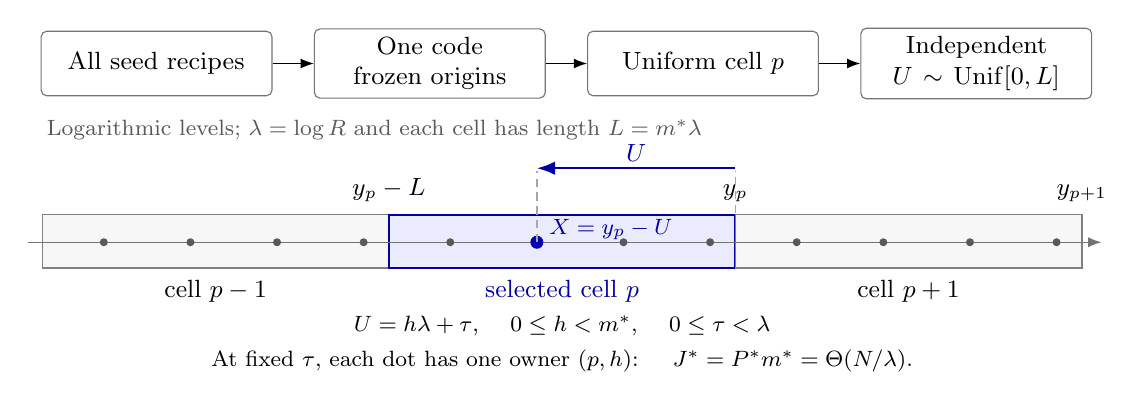
\begin{tikzpicture}[
  x=1cm,y=1cm,>=Latex,font=\small,
  processbox/.style={draw=black!55,rounded corners=2pt,align=center,
    minimum height=.82cm,text width=2.72cm,inner sep=3pt},
  cell/.style={draw=black!50,line width=.55pt},
  selected/.style={draw=blue!65!black,fill=blue!8,line width=.8pt},
  guide/.style={draw=black!35,densely dashed,line width=.45pt},
  every node/.style={inner sep=2pt}
]
\node[processbox] (recipes) at (1.65,3.62) {All seed recipes};
\node[processbox] (code) at (5.12,3.62) {One code\\frozen origins};
\node[processbox] (choose) at (8.59,3.62) {Uniform cell $p$};
\node[processbox] (view) at (12.06,3.62) {Independent\\$U\sim\mathrm{Unif}[0,L]$};
\draw[->] (recipes) -- (code);
\draw[->] (code) -- (choose);
\draw[->] (choose) -- (view);

\node[anchor=west,font=\footnotesize,text=black!65] at (.18,2.78)
  {Logarithmic levels; $\lambda=\log R$ and each cell has length $L=m^*\lambda$};
\draw[cell,fill=black!3] (.2,1.02) rectangle (4.6,1.70);
\draw[selected] (4.6,1.02) rectangle (9.0,1.70);
\draw[cell,fill=black!3] (9.0,1.02) rectangle (13.4,1.70);
\node[anchor=north] at (2.4,.94) {cell $p-1$};
\node[anchor=north,text=blue!65!black] at (6.8,.94) {selected cell $p$};
\node[anchor=north] at (11.2,.94) {cell $p+1$};
\node[anchor=south] at (4.6,1.79) {$y_p-L$};
\node[anchor=south] at (9.0,1.79) {$y_p$};
\node[anchor=south] at (13.4,1.79) {$y_{p+1}$};
\draw[->,draw=black!55] (.02,1.35) -- (13.65,1.35);

\foreach \x in {.98,2.08,3.18,4.28,5.38,6.48,7.58,8.68,9.78,10.88,11.98,13.08}
  \fill[black!65] (\x,1.35) circle (1.45pt);
\fill[blue!70!black] (6.48,1.35) circle (2.35pt);
\draw[guide] (6.48,1.35) -- (6.48,2.26);
\draw[guide] (9.0,1.72) -- (9.0,2.26);
\draw[->,draw=blue!65!black,line width=.8pt]
  (9.0,2.29) -- (6.48,2.29)
  node[midway,above,text=blue!65!black] {$U$};
\node[anchor=west,text=blue!65!black,font=\footnotesize] at (6.56,1.51)
  {$X=y_p-U$};

\node[align=center,font=\footnotesize] at (6.8,.06)
  {$U=h\lambda+\tau$, \quad $0\le h<m^*$, \quad $0\le\tau<\lambda$\\[3pt]
   At fixed $\tau$, each dot has one owner $(p,h)$:
   \quad $J^*=P^*m^*=\Theta(N/\lambda)$.};
\end{tikzpicture}
\caption[One code and a uniform coarsened view]{%
Sampling in Lemma~\ref{view:all-seed-code}, with the sequence index omitted.
All seed recipes are chosen before the independent chronological grid
shift, the common address code, and origin rounding.
The uniform cell and coarsening are sampled afterwards; the selected
time origins remain fixed as $U$ varies.
The dots show the coarsened levels at one fixed fractional phase
$\tau=U\bmod\lambda$.  Each is assigned to one seed cell, so the
$O(N)$ code budget is averaged over $J^*$ trials.
All complete cells participate, including those assigned the fallback
recipe.}
\label{fig:seed-coarsening}
\end{figure}


\begin{proof}
\emph{Seed recipes and one code.}
Fix the address ratio $R$ of Definition~\ref{arm:address-forest}, and put
$\lambda=\log R$.  Round $L_j$ to an integer multiple
$m_j^*\lambda$, retaining $L_j\to\infty$ and
$L_j=o(T_j\wedge\log H_j)$.  Sample an independent logarithmic mesh
displacement $V_j\sim\operatorname{Unif}[0,L_j)$.  Retain the complete
cells $[y_p-L_j,y_p]$ in $I_j$, where the endpoints $y_p$ run through
this translated mesh.  Their number $P_j^*$ satisfies
$P_j^*L_j=T_j+O(L_j)$.

At \emph{every} $y_p$, run exactly the deterministic greedy-center and
earliest-edge recipe in Proposition~\ref{view:saturation}, with the
same fixed orderings and diagonal cutoffs.  Temporarily truncate at an
integer $d_j$: retain the recipe only if its center count, all access
depths, all earliest-edge witness depths, and all witness-endpoint
distances from their assigned centers in seed units are at most $d_j$.
Otherwise replace that seed's list by the first distinguished base.
Include every access chain, every chosen actual colored link, and a
time-jump entry associating each endpoint of an earliest-edge witness
with its assigned seed center.  The latter jump has length at most
$d_jr_j(y_p)$.  These entries record the same center labels as the
saturated graph, rather than merely their separate access from bases.
There are at most $2\binom{d_j}{2}$ colored bits, and each access chain
has at most $d_j$ entries.  Thus a deterministic bound
$\Lambda_j=C(d_j+1)^3$ bounds the total marker and edge entries per
seed and its jump tolerance.  It includes the distinguished base names.

The enclosing chronological interval is part of the master event in
Lemma~\ref{view:macroscopic-cutoffs}.  Use its window indexed by a
deterministic composition bound $b(d_j)$ for all the retained access
chains, association jumps, and the finitely many current band requests.
Choose the actual cutoff slowly enough that $b(d_j)\le D_j$.
Write $\widehat C_j=C_{b(d_j)}$.  A seed leaving
$[-\widehat C_jn_j,\widehat C_jn_j]$ is also replaced by the base.
Every fixed recipe is eventually covered, since the selected laws
are already supported on the master event.  No ordinary
high-probability chronological bound is transferred through the growing
density bound in Equation~\eqref{view:selection}.

All lists have now been chosen, including the association jumps.
Only next sample the independent chronological grid displacement of
Definition~\ref{arm:address-forest}.  Form \emph{one} projected forest
from their union, marking every chain through its seed probe depth and
the distinguished bases through the final depth.  The seed depth is
rounded to the nearest address generation; its time unit differs by a
factor at most $R$, and different seeds still have distinct depths.
Round origins to the fixed even representatives inside their coded
terminal cells.  This is a function of the resulting code and grid;
it makes no new exploration or witness choice.  All projections of the
original chains and association jumps are already present at every
ancestor generation.

\smallskip\noindent\emph{Code and occupation budgets.}
Choose $d_j\to\infty$ sufficiently slowly that
\begin{equation}\label{view:all-seed-sparse}
 \frac{\Lambda_j\log(\Lambda_jL_j)}{L_j}\longrightarrow0.
\end{equation}
Also require
$\Lambda_j\log(2\widehat C_j)/L_j\to0$, by slowing $d_j$ further.
At each fixed cutoff the address root interval is a fixed multiple
of $n_j$, as required in Definition~\ref{arm:address-forest}.
Along the diagonal its enlarged root interval adds at most
$O(1+\log_R(2\widehat C_j))$ ancestors per marker.  The crude total
extra occupancy and code cost is therefore
$O(\Lambda_j(N_j/L_j)\log(2\widehat C_j))=o(N_j)$.
For every fixed ancestor padding $g$, the total number of markers and
the structural deletion error are then
\[
 M_j\le \Lambda_jP_j^*+O(1)
       =O(\Lambda_jN_j/L_j)=o(N_j),\qquad
 C_{R,g}M_j=o(N_j).
\]
Lemma~\ref{arm:jump-errors} bounds the integrated jump error by
$O_R((1+\log_R\Lambda_j)\Lambda_jN_j/L_j)=o(N_j)$.
This count includes the endpoint-association jumps.  Write
$\mathsf T_j$ for the forest's total occupied-node count.  The exact
code-count bound of Lemma~\ref{arm:address-codes} is
\[
 (\lambda+C_0)\mathsf T_j+
 \Lambda_jP_j^*\log(1+\mathsf T_j/P_j^*)+
 C P_j^*\Lambda_j\log(\Lambda_j+1)+O(\log(\mathsf T_j+1)).
\]
Equation~\eqref{view:all-seed-sparse} and
Equation~\eqref{arm:address-code-formbound} bound this by
$C_R\mathsf T_j+o(N_j)+O(1)$.  Proposition~\ref{arm:occupancy-tail}
applies to these simultaneous lists before the grid displacement;
its constant is independent of the fixed list cutoff.  Its exponential
tail and Equation~\eqref{view:selection} give
\begin{equation}\label{view:all-seed-budget}
 E_{Q_j}\mathsf T_j=O(N_j),\qquad
 E_{Q_j}\ell_j(C_j)=O(N_j).
\end{equation}
The Kraft code includes its occupancy-size cost.  Enlarging the slow
diagonal keeps these estimates and every prescribed fixed-cutoff
convergence.  No event requiring \emph{all} seed recipes to pass their
truncation has been conditioned on.

\smallskip\noindent\emph{The selected view law.}
Choose $p$ uniformly among the $P_j^*$ complete cells and,
independently, $U_j\sim\operatorname{Unif}[0,L_j]$.  Set
$Y_j=y_p$ and $X_j=Y_j-U_j$.  Averaging the independent mesh displacement
and the uniform cell makes the law of $Y_j$ differ from the uniform law
on $I_j$ by $O(L_j/T_j)$ in total variation, jointly with the word and
all its single-seed recipe data.  To see this, extend a bounded test
function by zero outside $I_j$ and average its mesh sum; every interior
point receives density $1/(P_j^*L_j)$, and the discarded end intervals
have total length at most $2L_j$.  The denominator differs from $T_j$
by at most $2L_j$.  The mesh is independent of the word.  Tightness of
the single-seed center count, first witness depths, and centered
endpoint offsets therefore makes the probability of fallback at this
uniformly selected seed tend to zero as the cutoffs are exhausted.
This proves the claimed equality of selected laws up to vanishing
error.  Choosing only among successful seeds would not have this property.

\smallskip\noindent\emph{One trial at each generation.}
Write
\[
 U_j=h\lambda+\tau,\qquad
 h\in\{0,\ldots,m_j^*-1\},\quad \tau\in[0,\lambda).
\]
The phase $\tau$ is independent of the entire code and is sampled
after it.  Conditional on this phase and the mesh, the pair $(p,h)$
is uniform on $P_j^*m_j^*$ possibilities.  The levels
$y_p-h\lambda$ are all distinct consecutive address generations,
up to their common fixed fractional phase.  Consequently
\begin{equation}\label{view:all-seed-level-count}
 J_j^*=P_j^*m_j^*=\Theta(N_j/\lambda).
\end{equation}
At such a generation use the frozen origins belonging to its unique
seed cell.  Distinct selected centers are separated by
$H_je^{-L_j}\to\infty$ in viewing units, so they occupy distinct
location nodes for all large $j$.  A fallback uses only one base.
Thus the selected center occurrences inject into occupied forest
nodes at each generation.  One does not count a new copy of a node
for each other seed whose chain also projects there.

\smallskip\noindent\emph{Central oscillations.}
Corollary~\ref{arm:central-oscillations} and
Equation~\eqref{view:all-seed-budget} give
$E_{Q_j}\sum_vS_v=O(N_j)$ for the same forest.  The injection of the
selected centers into its nodes and division by $J_j^*$ give the
asserted bounded first moment of the selected central amplitudes.
The estimate holds on every fixed enlargement of the selected time
neighborhoods.  In particular, normalized start-height differences
between blocks on the same line are tight before any passage transfer
or continuity conclusion is used.

\smallskip\noindent\emph{Disjoint slots and entropy transfer.}
For a fixed finite band request, use the enlarged bands of
Remark~\ref{arm:coarsened-bands}.  The bounded phase factor $e^\tau$
and the bounded seed-depth rounding factor only change their fixed
inner and outer radii.  Remove a fixed number of generations near
each seed endpoint; their selected probability is $O(1/L_j)$.
The terminal rounding and association offsets then vanish in view
units: for example
$Q_j(d_je^{-U_j}>\epsilon)\le
\log^+(d_j/\epsilon)/L_j\to0$.
For each fixed residue class with sufficiently spaced generations,
the regular-node construction gives disjoint enlarged chronological
slots.  Use an arbitrarily large \emph{fixed} ancestor depth $g$ in
that construction.  Its boundary-deletion proof gives, for a constant
$C_{A,R}$ depending on the requested bands,
\[
 \frac{E_{Q_j}\{\text{deleted selected center occurrences}\}}{J_j^*}
 \le o_j(1)+C_{A,R}R^{-g}
              \frac{E_{Q_j}\mathsf T_j}{J_j^*}.
\]
Indeed, conditional on the marker list, boundary loss is bounded by
a constant times $R^{-g}$ times the occupancy of a fixed reference
grid, which is within a factor two of every displaced-grid occupancy.
The structural loss is $C_{R,g}M_j=o(N_j)$.  Sending $j\to\infty$
first and then $g\to\infty$ makes the selected deletion probability
arbitrarily small, with $R$ and the underlying view law unchanged.

Given the code and the independent side information, all surviving
slot boundaries are fixed.  For one fixed residue, group these disjoint
raw slots by their trial $(p,h)$, assigning no slots to a deleted
request.  Let $h_i$ be the expected relative entropy of the $i$th
chronological raw-slot kernel, conditional on the code and its entire
preceding raw history, relative to a fresh iid block.  Averaging over
the code, Lemma~\ref{arm:entropy-allocation} gives
\[
 \sum_i h_i\le B_j:=\kappa_j+E_{Q_j}\ell_j(C_j)=O(N_j).
\]
There is a direct comparison retaining incoming stacks.  For a trial
$t=(p,h)$ with slot set $S_t$, keep the selected law's code marginal
and all its chronological gap and nonselected-slot kernels, but
replace precisely the kernels in $S_t$ by fresh iid blocks.  Call this
comparison $R_{j,t}$.  If $H_i(C_j,\mathcal H_i)$ is the conditional
relative entropy before slot $i$, so that $h_i=E_{Q_j}H_i$, the
chronological chain rule gives
\[
 D(Q_j\Vert R_{j,t})
 =E_{Q_j}\sum_{i\in S_t(C_j)}H_i(C_j,\mathcal H_i).
\]
Keep the code-dependent trial membership inside this expectation.
Use finite observations first and then increase the observed history.
Under $R_{j,t}$,
each requested slot is fresh conditional on its actual incoming history,
so the reference domination of Proposition~\ref{loc:slot-domination}
applies on each fixed compatible-instruction subevent.  No joint
conditioning on future gap histories is made; such
histories could encode the earlier target slots.

Sum over trials and then the fixed finite residue classes, and divide
by $J_j^*$ in Equation~\eqref{view:all-seed-level-count}.  Every slot
belongs to at most one trial within its residue, so the mean comparison
entropy is $O(1)$.  The denominator counts all seed-generation trials,
including deleted or empty requests.  Averaging over trials counts each
generation once, regardless of its number of lines.  This comparison
includes any fixed finite family of the
selected lines.  Lemma~\ref{view:entropy-null}
and the reference-slot domination transfer null tests on every fixed
compact range of retained shifts, on those compatible-instruction
subevents.  Whenever these shifts are tight under the selected law,
the compact restriction can then be removed.  The separate
continuum argument in Lemma~\ref{view:contour-slot-transfer} below
requires no flexible-order instruction.
First send the reference failure probability to zero, and then remove
the arbitrary deletion probability.  This divides the
\emph{all-seed} code budget by order $N_j$ levels.

\smallskip\noindent\emph{Stationarity.}
All seed recipes, the code, and its rounded origins precede $U_j$;
conditioning on them leaves $U_j$ uniform.  The fixed-origin
total-variation estimate of Lemma~\ref{view:stationarity} is therefore
unchanged.
\end{proof}

\subsection{Continuum laws in fresh slots}

The raw-slot entropy comparison gives the first Brownian null-event
statements without compatible passage-chart instructions.  A fresh band
before each retained block supplies a Gaussian increment to its starting
height.  We use this smoothing only for continuum paths and heights;
exact lattice observations will require the separate guarded comparison.

\begin{lemma}[Continuum transfer through fresh safety bands]
\label{view:contour-slot-transfer}
Consider a fixed finite list of chronological disjoint raw-word slots
at a common time scale $r_N\to\infty$.  Their boundaries and retained
block cuts are fixed by a code and auxiliary side information before
the fresh letters are sampled.  Each retained block has a left safety
band inside its slot whose rescaled duration is bounded above and
away from zero; retained durations satisfy the same bounds.
Let $R_N$ refresh these slots with iid raw words conditional on their
actual incoming histories, keeping all other chronological kernels
evaluated at the evolving past.

Record the retained increment paths and a fixed forest of relative
block-start heights in each coordinate, in units $\sqrt{r_N}$.
Every subsequential continuum law under $R_N$, restricted to finite
recorded differences, is locally dominated by independent Brownian
increment paths and independent forest differences with positive smooth
densities.  The reference retains the marginal law of the finite
duration and forest parameters.  Domination on a compact set of
differences is uniform in the incoming histories.

If selected laws $Q_N$ satisfy $D(Q_N\Vert R_N)\le H<\infty$,
also allowing this bound after adjoining and averaging the sampled
trial, their retained increment paths are tight and every joint
continuum limit has the same absolute continuity on finite differences.
The assertion applies to a selected subprobability on which those
differences are tight.  It is a statement about continuum contour
data, not about arbitrary scale-dependent lattice observations.
\end{lemma}

\begin{proof}
Fix the forest pattern.  In each of its components replace the tree
differences by differences from its chronologically earliest block.
This is an invertible integer linear change of coordinates with
determinant of magnitude one.  At each later block there is now at most
one new difference per coordinate, relative to an already observed
block.  A pattern chosen later can be handled by proving the assertion
for each fixed pattern and then restricting the limiting measures.

Anchor the contour before all slots.  Write $a_i^N$ for the beginning
of slot $i$, $u_i^N$ for its retained-block start, and $K_i\subseteq
\{1,2\}$ for the coordinates with a new difference.  If $p(i,c)<i$ is
the earlier block used in coordinate $c$, set
\[
 A_{i,N}^c=
 \frac{Z_c(a_i^N)-Z_c(u_{p(i,c)}^N)}{\sqrt{r_N}},
 \qquad
 G_{i,N}^c=
 \frac{Z_c(u_i^N)-Z_c(a_i^N)}{\sqrt{r_N}} .
\]
The first vector is measurable before the fresh slot.  The new
retained difference satisfies the exact identity
\[
 D_{i,N}=A_{i,N}+G_{i,N}.
\]
Let $X_{i,N}$ be the retained increment path, parametrized on $[0,1]$.
Proposition~\ref{arm:uniform-past-limit}, applied to the entire fresh
safety band and retained block, gives conditional bounded-Lipschitz
convergence
\[
 (G_{i,N},X_{i,N})\ \Longrightarrow\ (G_i,B_i),
 \qquad
 G_i\sim N(0,\tau_i\Sigma|_{K_i}),\quad B_i\sim\nu_{t_i}.
\]
Here $\Sigma$ is the Brownian covariance matrix, $\tau_i$ and $t_i$
are the limiting safety and retained durations, and $\nu_{t_i}$ is
the Brownian increment-path law of duration $t_i$.
The Gaussian $G_i$ and the path $B_i$ are independent.  Convergence is
uniform over incoming stacks and compact duration ranges: the
arbitrary-typing error is uniform, and deterministic restrictions and
time changes of the whole-slot limit give the displayed pair.  No
compatible flexible-order instructions are needed.

The density of $G_i$ is bounded uniformly because $\tau_i$ is bounded
away from zero.  Give the $K_i$-coordinate difference an independent
positive smooth reference density $p_i$.  For a nonnegative test $f$
supported on $|d|\le M$ and any translation $A_i$,
\[
 \mathbb E f(A_i+G_i,B_i)
 \le C_M\int f(d,x)p_i(d)\,dd\,\nu_{t_i}(dx).
\]
For bounded-Lipschitz tests the prelimit inequality has a uniform
$o(1)$ error.  Indeed translation by $A_i$ changes neither the bound
nor the Lipschitz constant of the test.  Empty $K_i$ requires only
the Brownian increment-path comparison.

Apply this bound to one nonnegative bounded-Lipschitz function of
\emph{all} retained outputs, supported on a compact set of their
differences.  Start at the last fresh slot and work backwards.
Earlier outputs are fixed at each conditional step.  Integrating the
current output against its independent reference law leaves a test
with the same bounded-Lipschitz control in the earlier outputs.
The intervening causal gap kernels integrate to one; they may depend
on earlier target slots, but their future realizations are never
conditioned on jointly.  This backward iteration bounds the limiting
expectation by a fixed multiple of the product Brownian and
smooth-height reference expectation, including the common parameter
marginal.  Bounded-Lipschitz approximation then gives local domination
of the joint continuum measures.

If a retained raw record includes a left extension before its used
start, place the fresh safety band before the entire record.  The
used-start difference is then exactly
$D=A+G+\Phi(X)$, where $\Phi$ is the retained extension's endpoint
evaluation.  Conditional on the retained Brownian path this is another
translation of the same Gaussian.  Endpoint evaluation is Lipschitz
in the uniform path metric, so the preceding argument is unchanged.

The comparison does not assume tightness of incoming heights.
Explicitly, on $|D_{i,N}|_\infty\le M$ and
$|A_{i,N}|_\infty>K$, the fresh safety fluctuation is at least $K-M$.
Proposition~\ref{arm:raw-exponential} and its deterministic oscillation
domination therefore give, uniformly over the incoming history,
\[
 R_N\bigl[|D_{i,N}|_\infty\le M,\
              |A_{i,N}|_\infty>K\bigr]
 \le C e^{-c(K-M)},\qquad K>M.
\]
With a used-start extension, apply the same bound to the safety band
and retained prefix together.  Thus escaped incoming heights produce
no unaccounted mass at finite retained differences.

Finally compactify the recorded differences to $[-\infty,\infty]$.
The retained path laws are tight under $R_N$ by the uniform fresh-slot
limit, and under $Q_N$ by the binary entropy bound.  First adjoin the
sampled trial under both laws; their common trial marginal turns the
averaged bound into joint entropy.  Then apply data processing to the
finite duration and forest parameters, retained paths, and compactified
differences, projecting away the trial identifier.  A joint weak
extraction of these two observation laws gives, by lower semicontinuity
of relative entropy,
\[
 D(Q^{\rm obs}\Vert R^{\rm obs})\le H<\infty,
 \qquad Q^{\rm obs}\ll R^{\rm obs}.
\]
The finite-difference part of $R^{\rm obs}$ has the local domination
proved above.  Exhausting finite compact difference sets proves the
selected assertion.  For a restriction by an additional event, adjoin
its indicator in the extraction; its limiting observation submeasure
is bounded by $Q^{\rm obs}$ and inherits the same absolute continuity
on its finite-difference part.  Undo the forest coordinate change.
Countably many buffered requests give the simultaneous off-origin
null-event assertions used below.  This reasoning uses weak limits of
contour paths; it supplies no prelimit domination for discontinuous
lattice passage costs.
\end{proof}

\subsection{Frozen origins and dilation stationarity}

We next extract the contour profiles around the chosen centers.  Their
origins are fixed before the viewing radius changes.  This gives a
stationary dilation law and, together with the oscillation estimate,
continuity even at a selected origin.

The all-seed construction supplies two different controls for this step.
The expected sum of the selected central oscillations is bounded.  For
each fixed off-origin band request, the selected experiment also has
bounded average relative entropy with respect to the trial law
$R_{j,t}$, which refreshes only the requested slots and leaves the other
chronological kernels unchanged, evaluated at the evolving past.
We first use the fresh-slot Brownian limit to control continuum
increments and finite relative heights.  Exact lattice passage
observations will additionally require the compatible-instruction
domination of Proposition~\ref{loc:slot-domination}.  For the later
annular crossings we must also express each test using only the retained
data and prove that those data admit an ordinary filling of positive
weight.  The following extraction establishes the contour and height
control needed for these geometric steps.

For a finite ordered list of times $\mathbf t=(t_1,\ldots,t_k)$ and a pair of
contours $Z$, define the centered paths at time unit $r$ by
\[
 Z^{i,r}(u)=r^{-1/2}\bigl(Z(t_i+ru)-Z(t_i)\bigr).
\]
The view also records the relative center heights in each coordinate in
$[-\infty,\infty]$, the quantities
$r^{-1/2}(\min_{[t_i,t_\ell]}Z^c-Z^c(t_i))\in[-\infty,0]$ for every
ordered center pair and coordinate $c$, and the closed scalar minimum relations on every finite
collection of bounded time windows.  Chronological ordering labels the
lines.  Dilation never changes these labels.  On a fixed line count the
dilation action is
\[
 (\mathcal D_v Z)^i(u)=e^{-v/2}Z^i(e^v u),\qquad
 \mathcal D_v H_{i\ell}=e^{-v/2}H_{i\ell}.
\]
The relation data are transformed by the same change of time variables.

\begin{lemma}[Uniform coarsening with fixed origins]\label{view:stationarity}
Let a seed level $Y_j$, a word, and a finite origin list $\mathbf t_j$ be
sampled first, with arbitrary dependence.  Independently sample
$U_j\sim\operatorname{Unif}[0,L_j]$, where $L_j\to\infty$, and form the view
at time unit $r_j(Y_j-U_j)$.  For every fixed $v\in\mathbb R$, its law and
the law of its $\mathcal D_v$ transform differ in total variation by at
most $|v|/L_j$, provided both are defined.  If boundary truncation fails with
probability $\delta_j$, add $2\delta_j$ to this bound.  Every weak limit on
which the dilation action is continuous is dilation stationary.
\end{lemma}

\begin{proof}
Condition on everything sampled before $U_j$.  Replacing the time unit by
$e^v$ times itself replaces $U_j$ by $U_j+v$, with the same origins.
Uniform measures on $[0,L_j]$ and $[v,L_j+v]$ differ in total variation by
at most $|v|/L_j$.  Pushforward cannot increase total variation.  Integrate
the conditional inequality and remove the boundary exceptional events.
For a weak limit, test bounded continuous functions and their compositions
with $\mathcal D_v$.  First take rational $v$; continuity gives all real $v$.
\end{proof}

The freezing of the origins is necessary.  For example, let
$f(t)=\sqrt{|t|}$, set $r=e^{-Y}$ and choose $t(Y)=r$.  Then
$[f(t(Y)+ru)-f(t(Y))]/\sqrt r=\sqrt{|1+u|}-1$ for every $Y$.
Uniform sampling of $Y$ therefore gives a constant law which is not dilation
stationary.  Lemma~\ref{view:stationarity} keeps the origins fixed during
coarsening, while Proposition~\ref{view:saturation} ensures that they
continue to cover the required exploration.

\begin{lemma}[Consequences of pinned stationarity]\label{view:signs}
Let a finite chronologically labeled line system have a dilation-stationary
law.  Assume its centered coordinate paths are continuous, and assume that
on each line distinct off-origin local minima of one coordinate almost
surely have distinct heights.  Then:
\begin{enumerate}[label=(\roman*)]
\item every recorded center-height difference belongs to
$\{-\infty,0,+\infty\}$ almost surely, and every recorded normalized
whole-center-gap minimum belongs to $\{-\infty,0\}$;
\item on each time half-line, a coordinate either is strictly positive
everywhere relative to its value at the origin, or takes strictly negative
values arbitrarily close to the origin;
\item if a coordinate is strictly positive sufficiently far out on a
half-line, it is strictly positive on the entire open half-line.
\end{enumerate}
These conclusions hold simultaneously for the finite random system.
\end{lemma}

\begin{proof}
For (i), the law of $H$ equals the law of $e^{-v/2}H$.  The disjoint geometric
annuli $(e^m,e^{m+1}]$, $m\in\mathbb Z$, have equal probability.  Each
therefore has probability zero.  Apply the same argument to $-H$, and to
each normalized minimum, which transforms by the same scalar multiplier.

Consider the positive half-line and put
$\tau=\inf\{t>0:Z(t)<0\}$, with the infimum of the empty set equal to
$\infty$.  Its law is invariant under multiplication by $e^v$, so
$\tau\in\{0,\infty\}$ almost surely by the same argument.  If $\tau=\infty$,
the path is nonnegative.  Any zero at positive time is then a local minimum.
There can be at most one such zero, by the distinct-minima hypothesis.
The time of that sole zero, if it exists, again has a multiplicatively
invariant distribution on $(0,\infty)$, so it cannot exist.  This proves (ii).
For (iii), apply the argument to
$\sup\{t>0:Z(t)\le0\}$, with the empty-set convention zero.  Eventual strict
positivity makes this supremum finite, so invariance forces it to be zero.
Reflect time for the other half-line.  Truncate the line count, apply the
argument to each coordinate and each label, and then remove the truncation.
\end{proof}

The distinct-minima hypothesis follows from joint off-origin Brownian
absolute continuity on countably many separated compact intervals.
The next Lemma establishes continuity at the origins, and
Lemma~\ref{view:returns} identifies the limiting center contacts.

\begin{lemma}[Continuity at the frozen origins]\label{view:origin-continuity}
Use the all-seed sampling construction of Lemma~\ref{view:all-seed-code}.
Suppose the code and oscillation estimates on that marked address list give
$E_{Q_j}\sum_v S_v\le C N_j$, where the sum runs over its projected
nodes and $S_v$ is the contour oscillation on a fixed enlargement of the
node box divided by the square root of its time radius.  Suppose also
that the disjoint-slot entropy estimate applies to every fixed finite
family of time bands at positive distance from the rounded origins and
to their recorded forest shifts.  Then the finite-line extraction can
be made with continuous centered contours.  On off-origin blocks,
every joint continuum law of increments and any recorded forest of
tight finite relative heights is absolutely continuous with respect
to independent Brownian blocks and smoothly distributed forest
differences.  In particular the
dilation-stationary limit satisfies Lemma~\ref{view:signs}.
\end{lemma}

\begin{proof}
\emph{Amplitude and off-origin control.}
Division by the order-$N_j$ trial count in
Equation~\eqref{view:all-seed-level-count}, using the selected-node
injection of Lemma~\ref{view:all-seed-code}, bounds the expected sum
over lines of the normalized oscillations on every fixed enlargement.
The projected boxes contain the rounded origins and the requested
bounded time intervals.  Thus, for every fixed $A<\infty$,
the centered amplitudes on $[-A,A]$ are tight.  Relative start heights
between blocks on the same line are differences of these amplitudes
and are tight as well.  This is the source of the compact height
truncation; it is not an inference about the entire selected past.

Truncate the line count and fix finitely many bands with rational
endpoints avoiding zero.  Coarse rounding errors are covered by slightly
enlarging these bands.  Along each unary part of the projected address
tree, choose a fixed residue class of logarithmic levels sufficiently
spaced that their enlarged bands are disjoint.  Increase the ancestor
padding by the fixed amount required for these bands.  The regular-slot
estimate has arbitrarily small deletion probability by the fixed-padding
exhaustion in Lemma~\ref{view:all-seed-code}; the residue is chosen
uniformly and independently, preserving the level marginal.  Conditional
on the code and independent phase, the surviving raw-word slots have
fixed disjoint boundaries.  Give each tested block a deterministic left
safety band of positive rescaled duration within its enlarged off-origin
slot.  Apply Lemma~\ref{view:contour-slot-transfer} to the freshened
trial experiment of Lemma~\ref{view:all-seed-code}.  It gives punctured
compact-uniform tightness and joint continuum absolute continuity
without choosing flexible-order instructions.  The Gaussian safety
increment smooths each new forest difference; the following retained
increment path is Brownian in the reference limit.  The bounded average
trial entropy transfers its null events.  Tightness of the tested
finite differences allows their compact ranges to be exhausted.
The same argument applies to every additional fixed forest whose
differences are tight on the restricted subprobability under study.
Exact lattice observations will instead use
Proposition~\ref{loc:slot-domination} on compatible protected charts
later in the argument.

\smallskip\noindent\emph{Control at the origins.}
For the fixed unit enlargement write the preceding expectation bound
as $C'$, and put
$M_j(\delta)=\sum_i\sup_{|u|\le\delta}|Z_j^i(u)|$.
Apply Lemma~\ref{view:stationarity} before taking a limit.  For fixed
$\delta,\epsilon>0$, scaling the frozen view by $\delta$ gives
\[
 Q_j[M_j(\delta)>\epsilon]
 \le Q_j[M_j(1)>\epsilon/\sqrt\delta]
       +O(|\log\delta|/L_j)+o_j(1)
 \le C'\sqrt\delta/\epsilon+O(|\log\delta|/L_j)+o_j(1).
\]
Thus $\lim_{\delta\downarrow0}\limsup_j
Q_j[M_j(\delta)>\epsilon]=0$.  Together with tightness on punctured
compacts, this is full compact-uniform tightness, including the origins.
It excludes narrow prelimit spikes which punctured convergence alone
would miss.  In a joint subsequential limit, Fatou's lemma gives
\[
 E\sum_{i=1}^K\sup_{0<|u|\le1}|Z^i(u)|\le C'.
\]
Lemma~\ref{view:stationarity} applies on the punctured-line path space.
Consequently, for $0<\delta<1$,
\[
 E\sum_{i=1}^K\sup_{0<|u|\le\delta}|Z^i(u)|
 =\sqrt\delta\,E\sum_{i=1}^K\sup_{0<|u|\le1}|Z^i(u)|
 \le C'\sqrt\delta.
\]
The left-hand suprema decrease as $\delta\downarrow0$, so their limits
are zero almost surely.  Set $Z^i(0)=0$.  This proves continuity at every
origin, together with the already obtained continuity elsewhere.
Countably many bands, increasing line truncations, and the original
packing and graph statistics can all be included in the same diagonal.
\end{proof}

\begin{corollary}[Tightness of retained height differences]
\label{view:finite-shift-groups}
In the preceding stationary extraction, fix a coordinate and group
centers whose normalized height differences have finite limits.
Within each such group those limits are zero.  Every finite forest
of relative start heights between retained off-origin blocks in the
group is tight, and its joint continuum law with the block increments
has the reference absolute continuity of
Lemma~\ref{view:origin-continuity}.
\end{corollary}

\begin{proof}
Write $Z_j$ for the chosen scalar contour, $c_{j,i}$ for a center,
and $r_j$ for the viewing time unit.
For block starts at coordinates $u$ and $v$ on lines $i$ and $\ell$,
their normalized height difference is
\[
 r_j^{-1/2}\bigl(Z_j(c_{j,\ell})-Z_j(c_{j,i})\bigr)
       +Z_j^\ell(v)-Z_j^i(u).
\]
The first term tends to zero within a finite relative-height group
by Lemma~\ref{view:signs}(i).  The remaining terms are tight by the
compact centered-profile bounds.  For a random group pattern, these
assertions concern the corresponding restricted subprobability law;
stationarity is used under the original law before this restriction.
After truncating the line count
there are finitely many group and forest choices; applying the
off-origin transfer to each gives the joint assertion.  No finite
relative height between different groups is needed.
\end{proof}

\subsection{First returns and protection of omitted gaps}

Use a joint contour coupling after Proposition~\ref{view:saturation} and
Lemma~\ref{view:origin-continuity}.  Write $c_{j,i}$ for the ordered
centers and $r_j=r_j(X_j)$.  Record center differences and all intervening
minima in the extended real line.  Centers $i<\ell$ have a scalar center
contact when their normalized height difference tends to zero and
\begin{equation}\label{view:center-contact}
 \liminf_j r_j^{-1/2}
 \left(\min_{[c_{j,i},c_{j,\ell}]}Z_j-Z_j(c_{j,i})\right)\ge0.
\end{equation}
For a given coordinate these contacts form the ordinary scalar contour
equivalence relation on the finite ordered center set.  Every scalar
center class lies in one finite relative-height group, so
Corollary~\ref{view:finite-shift-groups} applies to its retained blocks.
Our next task is to realize its contacts by actual lattice chords and
to keep the omitted chronological gaps strictly above the tested levels.

\begin{lemma}[Actual return witnesses and whole-gap clearance]
\label{view:returns}
Assume each bilateral scalar contour eventually returns below each fixed
level in either time direction.  In the saturated stationary system:
\begin{enumerate}[label=(\roman*)]
\item Every strictly positive half-line faces another member of the same
scalar center class.  Each inward half-line of a scalar class is strictly
positive and its two outward half-lines have negative values arbitrarily
near their origins.
\item Consecutive members of each scalar class are joined by actual
lattice chords whose endpoints approach the corresponding origins in
view units.  Thus the scalar rank of the center class is witnessed by
the simultaneously saturated actual-link graph.
\item Fix positive neighborhoods of all enrolled origins within their
retained line intervals.  Between consecutive members of a scalar center
class, after removing those neighborhoods, the scalar height has positive
clearance above the class height on the whole omitted chronological gap,
in probability: its normalized positive margin has tight reciprocal
after any fixed finite geometric truncation.
\end{enumerate}
\end{lemma}

\begin{proof}
Consider a positive right half-line of center $i$ and fix a departure
time $d>0$.  Choose deterministic $\epsilon_j\downarrow0$ sufficiently
slowly to dominate contour errors on every currently fixed compact and
the vanishing differences of tied center heights.  Round
$Z_j(c_{j,i})+\epsilon_j\sqrt{r_j}$ to an attainable scalar lattice level
$h_j$.  Its rounding error divided by $\sqrt{r_j}$ vanishes.  Let $a_j$
be the last visit to $h_j$ before $c_{j,i}+dr_j$, and let $b_j$ be the first
visit thereafter.  The first exists because the center height is below
$h_j$ and the departure height is above it; the second exists by bilateral
recurrence.  The last/first convention gives
\[
 Z_j(a_j)=Z_j(b_j)=h_j,
 \qquad \min_{[a_j,b_j]}Z_j=h_j.
\]
This is an actual scalar chord.  Strict positivity on each compact
$[\eta,d]$ implies $(a_j-c_{j,i})/r_j\to0$.

The first endpoint is reached by one bounded jump, and the second by
one chord.  Universal coverage in
Equation~\eqref{view:uniform-target-coverage} therefore puts $b_j$ within
a tight coordinate range of an enrolled line.  Choose a joint convergent
subsequence of its label and coordinate, denoting the latter by $y$.
The receiving line cannot be $i$, by positivity on all its positive
compacts.  It is a later line, say $\ell$.  The equality at $b_j$ shows
that the center-height difference is finite; Lemma~\ref{view:signs}(i)
makes it zero, and the receiving profile satisfies $Z^\ell(y)=0$.
Every finite receiving coordinate $u<y$ occurs between the departure and
the return for large $j$, so $Z^\ell(u)\ge0$.

We claim $y=0$.  If $y<0$, nonnegativity on $(-\infty,y)$ and distinct
off-origin minima imply strict positivity sufficiently far to the left;
Lemma~\ref{view:signs}(iii) then gives strict positivity on the entire
left half-line, contradicting $Z^\ell(y)=0$.  If $y>0$, nonnegativity on
$(0,y)$ rules out the negative-near-zero alternative on the right half;
strict positivity there again contradicts the zero.  Hence $y=0$ and the
receiving left half is positive.  The chord inequalities also give
Equation~\eqref{view:center-contact}, so $i$ and $\ell$ are in the same
scalar class.  Reflect time for a positive left half.

Conversely a center contact makes the corresponding inward half-lines
nonnegative, hence positive by Lemma~\ref{view:signs}.  A positive outward
half would, by the preceding return construction, produce an additional
class member beyond the extreme one.  The outward halves must therefore
have negative values arbitrarily near zero.  This proves (i).

For consecutive class members $i<\ell$, choose the errors $\epsilon_j$
also to exceed all their vanishing center-height differences.  The first
return from $i$ occurs before $c_{j,\ell}$, whose height is below $h_j$.
The preceding argument places any limiting return at an intermediate
center in the same class.  Consecutiveness forces it to be $\ell$, and
its coordinate tends to zero.  These are actual finite-reach witnesses.
Their finite union can be included in the edge extraction of
Proposition~\ref{view:saturation}.  This proves (ii), including the rank
$|A|-1$ from consecutive pairs of a scalar class $A$.

For (iii), suppose instead that a whole omitted gap has normalized
minimum approaching zero with probability bounded below.  Record that
event in a joint extraction, retaining the original unconditioned
stationary law; do not condition the stationary law on the event.
Take $\epsilon_j\downarrow0$ more slowly than this minimum and the
convergence errors.  Start the preceding chord search at a fixed
positive departure lying inside the retained interval before that gap.
Its first return must occur before the low point in the omitted gap.
By (ii), and by choosing the start after the last near-origin crossing
of $h_j$, every subsequential return approaches the next class center.
If the search encounters a retained intervening line, equality at the
return and the minimum inequality put its center into the same class;
consecutiveness excludes it.  More precisely, the offending low point
precedes $c_{j,\ell}-\eta r_j$ for the fixed radius $\eta>0$ of the
removed neighborhood of the next member $\ell$.  Hence
$b_j\le c_{j,\ell}-\eta r_j$, whereas the return argument in (ii),
applied with these same slowly decreasing heights, gives
$(b_j-c_{j,\ell})/r_j\to0$.  This is a contradiction.  Universal coverage
has already excluded escape between the enrolled lines or to an
unbounded coordinate on one of them.  This proves that the
whole-gap minimum is bounded away from zero after a probability
truncation.  There are finitely many classes and gaps on each truncation,
so their minimum margin has the same property.  Remove the truncations
and use a countable sequence of origin neighborhoods.
\end{proof}

\begin{corollary}[Interline partners belong to one scalar class]
\label{view:interline-class}
An actual scalar link whose endpoints have bounded coordinates on two
distinct enrolled lines has endpoints on lines in the same scalar center
class in every subsequential limit.
\end{corollary}

\begin{proof}
The equality of endpoint heights and bounded local contour oscillations
make the center-height difference finite, hence zero by
Lemma~\ref{view:signs}.  The chord lower bound, with the bounded end pieces
between endpoints and centers, bounds the normalized whole-center-gap
minimum from below.  Its limit is finite, hence zero by the same Lemma.
This is Equation~\eqref{view:center-contact}.
\end{proof}

\begin{lemma}[Protected completion of one center component]
\label{view:protected-completion}
Fix a finite combined center component from Lemma~\ref{view:returns}.
Retain sufficiently short closed intervals about all its center visits,
in their chronological order.  There is a pair of positive continuous
excursion contours on a finite interval containing translated copies of
all these retained profiles.  Its scalar center classes are exactly the
prescribed ones.  Each translation is common to a scalar class, and every
omitted connector satisfies strict lower inequalities protecting all
links sufficiently near the center class.  The component-height choices
and connector conditions range over a nonempty open set.  They can be
sampled with densities and Brownian bridges of the prescribed covariance.
\end{lemma}

\begin{proof}
Handle the two coordinates separately for the height assignment.  A
scalar partition of ordered contour visits is noncrossing: two
interleaving scalar contacts are at the same height and are one class.
Consequently class spans are nested or disjoint.  If $B$ lies between
consecutive members of $A$, impose $A\prec B$.  These finitely many
nesting inequalities have no cycle.  They also agree with the original
strict height ordering: the minimum inequality for $A$ makes a center
inside its span no lower than $A$; equality would make it a member of
$A$, so a distinct intervening class is strictly higher.  By stationarity
its original relative height is in fact $+\infty$ in view units.

Choose rational cuts on every retained half-profile.  On each outward
half retain a definite negative dip before its cut.  The two coordinates
need not have their negative dips at the same time; take the common cut
after both required dips.  Every inward half is positive at its cut.
Let $K_0$ bound all retained centered oscillations.  For each coordinate
choose a linear ordering of its classes extending nesting, with ranks
$s(A)\in\{1,\ldots,k\}$, and assign
\[
 H_A=(4K_0+10)s(A)+u_A,\qquad |u_A|<1.
\]
Give every profile of class $A$ this common added height.  All pieces
are positive.  Every enclosed class lies above an enclosing level by
more than $2K_0+8$.  The two coordinates have distinct height variables,
so these choices impose no cross-coordinate compatibility equation.
Equal heights of unrelated classes need not be retained.

Choose $\delta>0$ smaller than one quarter of the finitely many inward
cut heights, chosen outward dip depths, and original protected-gap
margins from Lemma~\ref{view:returns}.  Shrink the working neighborhoods
of the centers so all centered profile heights there have magnitude
less than $\delta$.  At a gap between consecutive retained intervals,
the classes whose spans cross that gap form a nested chain.  Both cut
values exceed every active class height by more than $2\delta$: a cut
in that class lies on its inward side, and every other relevant cut
belongs to a strictly enclosed class.  If no class spans the gap,
positivity is the only lower requirement.  Coordinatewise linear
interpolation joins the endpoint vectors while preserving these strict
bounds.  A small uniform tube about it does likewise.  Exterior tails
join to zero with positive interior values; ordinary quadrant-excursion
entrance and exit pieces can be used in place of deterministic tails.

Inward positivity and connector bounds join all members of a prescribed
scalar class at their common level.  Outward dips block any contact
leaving its span.  No additional zero-level contact occurs on a retained
half: inward halves are strictly positive and every outward interval
starting at the center contains a negative value.  Distinct scalar
classes have distinct assigned heights.  Thus the prescribed center
class is saturated under both scalar relations.  All inequalities use
strict margins, so the height variables may have a density supported in
the indicated open feasible box.  Brownian bridges have positive
probability of satisfying the connector tubes by
Lemma~\ref{view:positive-fill}.  Countably many rational cuts and margins
suffice for the choices.
\end{proof}

\subsection{Open fillings and crossing transfer}

The completed center profiles may have singular laws at their origins.
We will test passages only away from those times.  The next lemmas
explain why a strictly compatible ordinary filling transfers a null
event on the retained data, even if its filling probability is small.

Let $I_1,\ldots,I_m$ be finitely many disjoint closed intervals in a bounded
time interval, with positive gaps between them.  A block datum consists of
the increment path on each $I_i$ and, for each coordinate, height differences
along a forest on the set of blocks.  A forest supplies one independent
difference per non-root vertex, so its differences and one absolute height
per component parameterize all block-start heights bijectively.  No cyclic
list of redundant differences is assigned an independent density.

\begin{definition}[Open fillability]\label{view:fillable}
A finite recipe specifies finitely many strict inequalities on endpoint
heights, minima of omitted gaps, and minima or maxima of retained compact
subintervals.  The inequalities may depend continuously on the recorded
block datum.  A datum is openly fillable for the recipe if one can choose
the unrecorded component heights and continuous paths in the omitted gaps
so that every inequality holds.  The gap paths must have the endpoint
values prescribed by their adjacent blocks.  All interval lengths are
bounded above and away from zero on each compact parameter truncation.
\end{definition}

\begin{lemma}[Positive fill weight]\label{view:positive-fill}
Fix a nondegenerate two-dimensional Brownian covariance matrix.  Give the
unrecorded component heights an everywhere positive continuous density,
and conditionally fill each positive-length gap by the corresponding
Brownian bridge.  Every openly fillable datum has positive conditional
probability of satisfying the recipe.  Openly fillable data form a
measurable set which is a countable union of versions using rational
parameter boxes and rational polygonal approximations with a positive
inequality margin.
\end{lemma}

\begin{proof}
For a chosen filling, finitely many strict continuous inequalities have a
common positive margin.  A sufficiently small open box of component
heights and a sufficiently small uniform neighborhood of the chosen
continuous gap paths preserve that margin.  The height box has positive
probability.  A Brownian bridge with nondegenerate covariance has full
support on the continuous paths with its endpoints: approximate the chosen
path by a polygonal path, constrain the bridge at its finitely many
vertices using the strictly positive Gaussian density, and constrain its
bridge fluctuations on the remaining subintervals to a small uniform
ball.  Each of these probabilities is positive.  The same statement holds
uniformly on a sufficiently small box of endpoints, although no uniform
lower bound over all openly fillable data is asserted.  Independent filling
of finitely many gaps proves positivity.  Rational approximations to the
height boxes, polygonal paths, and margins give the last assertion.
\end{proof}

One may also require positivity in the quadrant on the interior filling
intervals, since it is an open condition on compact subintervals.  To obtain
an ordinary quadrant excursion, its initial and terminal pieces are
sampled from the ordinary excursion law, while the positive-time interior
gaps have the usual killed-bridge densities.  Their strictly positive
densities on the quadrant give the same support assertion.  This does not
condition free Brownian motion to reproduce any distinguished singular
center profile.

\begin{lemma}[Transfer on an openly fillable chart]\label{view:fillable-null}
Let $\nu$ be the reference law of the recorded block data, and let $K(v,do)$
be a probability kernel for the passage observations.  Suppose an ordinary
Brownian completion which realizes a fixed recipe induces the subprobability
law
\begin{equation}\label{view:completion-density}
 f(v)\nu(dv)K(v,do),\qquad f(v)>0\quad
 \text{for $\nu$-almost every openly fillable $v$}.
\end{equation}
If a measurable failure test $E$ has probability zero in that completion,
then
\[
 \int_{\{v:\,v\text{ openly fillable}\}}K(v,E_v)\,\nu(dv)=0.
\]
Consequently any sequence of selected chart experiments having tight
absolute continuity with respect to these reference experiments transfers
their vanishing failure probabilities.
\end{lemma}

\begin{proof}
The assumed null event says $\int f(v)K(v,E_v)\nu(dv)=0$.  The integrand is
nonnegative and $f$ is positive on the set in question.  For instance,
restrict to $f\ge1/k$ and let $k\to\infty$.  This gives the assertion.
The sequential version follows from the definition of tight absolute
continuity, or from Lemma~\ref{view:entropy-null} together with the required
iid reference domination.
\end{proof}

The positive filling density in Equation~\eqref{view:completion-density}
is supplied by Lemma~\ref{view:positive-fill}.  The common passage kernel
and feasible-lattice domination are supplied by the local-kernel
construction of Section~\ref{loc:section}.

\begin{lemma}[Off-center law of the completion]\label{view:completion-ac}
Suppose the original finite-line view has the joint off-origin absolute
continuity specified in Lemma~\ref{view:origin-continuity}, with all
forest differences within each scalar center class retained.  The completion
in Lemma~\ref{view:protected-completion} may be sampled so that every
finite collection of disjoint compact time intervals avoiding its
centers and common endpoint has joint absolute continuity with respect
to Brownian blocks with a full-density vector of absolute starting
heights.
\end{lemma}

\begin{proof}
First fix the countable choices of center labels, scalar center classes,
rational cuts, and inequality margins.  Restricting to the event of
this choice preserves every null assertion.  For blocks in retained
profiles, record a spanning tree of block-start differences within
each scalar center class, separately in each coordinate.  Their union
is a forest.  Each such class lies
in a finite relative-height group, so
Corollary~\ref{view:finite-shift-groups} supplies joint absolute
continuity of these differences and the block increments.  Discard
differences between distinct scalar center classes, even when their
center heights belonged to the same finite relative-height group before
completion.

For each scalar center class, adjoin the absolute start height of one
reference block.  Conditional on the retained profiles, this anchor is
a translate of that class's continuously randomized height and hence
has a density.  The within-class forest differences and one anchor per
class parameterize all block-start heights by an invertible linear map
with determinant of magnitude one.  Fubini's theorem gives absolute
continuity of all starts and increments jointly.  No Brownian conditional
law given a singular center profile is required.

Conditionally on the retained profiles and their heights, each filler is
a Brownian bridge restricted to an event of positive conditional
probability.  Its law is absolutely continuous with respect to the
unrestricted bridge with those endpoints.  Marginalizing any unused
central data preserves that absolute continuity.  Brownian bridge
disintegration across a deterministic cut identifies the resulting
reference measure on a neighborhood crossing the cut with a Brownian
restriction having the same start density.  Thus the assertion holds
also for intervals meeting seams.  The entrance and exit pieces have
the same local property away from the common endpoint.  Finally take
the countable union over recipe choices and rational windows covering
the requested compact intervals.
\end{proof}

\subsection{A deterministic sphere theorem for the completed contours}

We have protected the distinguished contacts.  We must also know that
the entire completed contour quotient is a sphere.  The following
deterministic criterion separates this topological question from the
passage-cost estimates: its two hypotheses are finite fibers and an
acyclic incidence graph within each fiber.

\begin{theorem}[Finite acyclic contour sewing]\label{view:moore}
Let $L,R:[0,T]\to[0,\infty)$ be continuous, zero at the endpoints and
strictly positive in between.  On the circle $\mathcal C=[0,T]/(0=T)$,
let $\sim_c$ be the scalar contour relation
\[
 s\sim_c t\quad\Longleftrightarrow\quad
 c(s)=c(t)=\min_{u\in[s,t]}c(u),\qquad c\in\{L,R\},
\]
with ordered representatives and the endpoint convention.  Let $\sim$ be
the relation generated by the two scalar relations.  Suppose:
\begin{enumerate}[label=(\roman*)]
\item a finite constant $M$ bounds the cardinality of every $\sim$-class;
\item for every $\sim$-class $E$, the bipartite multigraph with vertices the
$L$-classes and the $R$-classes in $E$, and one edge for each $t\in E$
joining its two scalar classes, is a tree.
\end{enumerate}
Then $\mathcal C/\sim$ is homeomorphic to the sphere.  The quotient map is
continuous and its fibers are exactly the $\sim$-classes.
\end{theorem}

\begin{proof}
Realize $\mathcal C$ as the unit circle by $z(t)=\exp(2\pi i t/T)$.  The
scalar relation is closed, since the interval minimum is a continuous
function of its endpoints.  Distinct scalar classes are unlinked: if
$s<t<u<v$, $s\sim_c u$, and $t\sim_c v$, the minimum inequalities imply
$c(s)\le c(t)\le c(u)=c(s)$, and all four points belong to one scalar
class.  Hence the closed convex hulls of distinct scalar classes are
disjoint.

We check that these hulls cover their closed disk; no unstated maximality
of a lamination is needed.  For a circular interval $[a,b]$ write
$K[a,b]=\operatorname{conv}(z([a,b]))$.  Suppose an interior point $w$ is
in no scalar-class hull.  For $h>0$, components $(a,b)$ of $\{c>h\}$ have
scalar-equivalent endpoints.  If $w\in K[a,b]$, it is in the interior of
that cap, since its chord edge is already in a class hull.  There is such
a cap at some positive $h$: a sufficiently long compact arc avoiding the
common endpoint contains $w$ in its cap and has positive minimum height.
Let $H$ be the supremum of these heights.  Along heights increasing to
$H$ the relevant components are nested.  Their limiting endpoints $a,b$
satisfy $c(a)=c(b)=H$, $c\ge H$ on $[a,b]$, and $w\in K[a,b]$.
The finite set $A=\{t\in[a,b]:c(t)=H\}$ is contained in one scalar class.
The cap $K[a,b]$ is the union of $\operatorname{conv}(z(A))$ and the caps
over successive complementary intervals of $A$.  Their separating edges
belong to the former hull.  Thus $w$, being outside that hull, lies in the
interior of a cap over an interval $(u,v)$ where $c>H$.  There are
$u<u'<v'<v$ with $w\in K[u',v']$; the positive minimum of $c-H$ on
$[u',v']$ gives a component cap containing $w$ at a height above $H$.
This contradiction proves coverage.  Singleton hulls cover any remaining
boundary points.

The generated relation is also closed.  If $s_n\sim t_n$ and
$(s_n,t_n)\to(s,t)$, join each pair by a simple monochrome chain of length
at most $M-1$.  Pad it with constant steps.  There are finitely many color
patterns; after choosing one pattern, compactness of the finite product
$\mathcal C^M$ supplies limits for all intermediate points.  Closedness of
the scalar relations gives a chain from $s$ to $t$.

Glue an $L$-disk and an $R$-disk along $\mathcal C$.  For a combined class
$E$, let $H_E$ be the union of its scalar hulls in the respective disks.
Coverage and disjointness show that these sets partition the sphere.
Each is a compact connected finite union of polygons, segments, and
points.  The decomposition relation on the sphere is closed: if
$x_n,y_n\in H_{E_n}$ converge, choose their containing hemispheres and
express each as a convex combination of at most three hull vertices.
After a subsequence all six vertices and their coefficients converge.
Each triple remains scalar-equivalent, and all six vertices remain
combined-equivalent by the closedness just proved.  The limits therefore
belong to one $H_E$.

Each $H_E$ is nonseparating.  A polygon can be strongly deformation
retracted, fixing its boundary vertices, onto the star from an interior
point to those vertices: triangulate from the interior point and collapse
each triangle onto its two radial sides.  These collapses agree where
triangles and hulls meet.  Segments and singleton hulls need no change.
The resulting finite graph is the subdivided bipartite incidence graph,
with the harmless contractions due to singleton hulls.  Hypothesis (ii)
makes it a tree.  Thus $H_E$ is contractible.  It is a finite planar
polyhedron, so Alexander duality gives
$\widetilde H_0(S^2\setminus H_E;\mathbb Z)=0$; its complement is connected.

We have a closed decomposition into compact connected nonseparating sets.
It is not the one-set decomposition, because its intersections with the
infinite circle have at most $M$ points.  Moore's sphere theorem in this
form, as stated in \cite[Theorem 1.1]{TimorinMoore}, gives a sphere quotient.
Every hull meets the circle, so the induced map from $\mathcal C/\sim$ is
a continuous bijection onto that sphere.  A continuous bijection from a
compact space to a Hausdorff space is a homeomorphism.
\end{proof}

\begin{remark}[The rank in the topological criterion]\label{view:rank-tree}
For a combined class $E$ of size $m$, let $v$ be its number of scalar
classes and let
$e=\sum_{A\text{ scalar class in }E}(|A|-1)$.  Every visit is counted once
in each color, so $e=2m-v$.  Its connected incidence multigraph has $m$
edges and $v$ vertices.  It is a tree exactly when $e=m-1$, and has a cycle
exactly when $e\ge m$.  This includes a two-edge cycle from a nontrivial
common chord.  Filled polygons are not themselves called trees; the
deformation argument in the proof is what converts the incidence condition
into nonseparation.
\end{remark}

\begin{corollary}[One distinguished class]\label{view:one-class}
In Theorem~\ref{view:moore}, suppose a finite distinguished set $S$ is
exactly one combined class, its incidence graph is a tree, and no scalar
relation joins $S$ to its complement.  Suppose on the complement of $S$
and the common endpoint there is joint Brownian absolute continuity on
every finite family of separated compact time intervals, including their
relative starting heights.  Then the completed quotient is a sphere.
\end{corollary}

\begin{proof}
By Lemma~\ref{arm:finite-diagram-polarity}, a separated off-center diagram
is polar when $\beta e>m$.  A rank cycle has $e\ge m$ and is therefore polar.
Choose an integer $m_0$ with $\beta(m_0-1)>m_0$.  A connected diagram with
$m_0$ distinct visits has $e\ge m_0-1$ and is also polar.  An equivalence
class with at least $m_0$ visits contains such a finite connected diagram:
start at one point and add new points successively along a monochrome
connection.  All its points lie in some finite family of disjoint rational
windows avoiding the distinguished times.  A countable union of the
polarity assertions therefore bounds every other class by $m_0-1$ and
excludes its cycles.  The distinguished set is saturated by assumption,
and the common endpoint is a singleton by strict positivity.  Apply
Theorem~\ref{view:moore} with
$M=\max\{|S|,m_0-1,1\}$.
\end{proof}

\begin{lemma}[Localizing an annulus by its finite fiber]\label{view:annulus-preimage}
Let $\eta:\mathcal C\to S^2$ be the quotient from
Theorem~\ref{view:moore}, and suppose $\eta^{-1}(z)=S$ is its finite
distinguished fiber.  For every open $J\subset\mathcal C$ containing $S$
there are nested closed topological disks about $z$, with an annular
margin between them, whose preimages lie in $J$.  The preimage of any
compact annulus avoiding $z$ is bounded away from $S$.
\end{lemma}

\begin{proof}
The compact set $\eta(\mathcal C\setminus J)$ excludes $z$.  Choose the
nested disks inside its open complement using a sphere chart at $z$.
For the last assertion, the annular preimage is compact and disjoint from
the finite fiber $S$.
\end{proof}

\subsection{Exact retained lattice patches}

We next transfer a disk around the distinguished point back to the
original map.  Both accepted and rejected scalar tests must be preserved;
retaining only the intended chords could create additional partners.
A retained interval carries its actual resolved steps.  Each
coordinate has a partition of the retained intervals into tied groups.
Within each group an auxiliary completion may translate that coordinate
by a common integer, preserving all its exact differences.  Parity
restrictions are imposed on these translations.  The auxiliary completion
may use arbitrary admissible filler steps in the omitted intervals.

\begin{lemma}[Exact incidence under protected gaps]\label{view:exact-incidence}
Consider an original and an auxiliary resolved contour sewing with the
same retained step intervals, up to the preceding group translations.
Let $T$ be a set of retained triangles together with all triangles incident
to their vertices and sides.  Suppose the following conditions hold for
every scalar relation needed to specify these incidences.
\begin{enumerate}[label=(\roman*)]
\item Every endpoint of the relation belongs to a retained interval, and
the endpoints belong to the same translation group for that coordinate.
\item Every intervening retained comparison is preserved: tied pieces
have the same heights relative to the tested height, and other intervening
pieces lie strictly above that height in both sewings.
\item Every omitted gap between its endpoints has minimum strictly above
the tested height in both sewings.
\item Every other candidate partner of a step or corner in $T$ is excluded
in both sewings, either by unequal endpoint heights or by a retained
value strictly below its tested height.
\end{enumerate}
Then the sewings have identical triangle, side, and vertex incidence on
$T$.  In particular, any embedded disk whose triangles and full vertex
stars are contained in $T$ transfers as a planar patch.  A circuit and its
chosen interior inside that disk transfer with their genuine all-edge
lengths unchanged.
\end{lemma}

\begin{proof}
A scalar contour identification is the equality of the endpoint heights
together with the statement that every intervening height is at least
their common value.  A step match is the corresponding adjacent-level
version.  Condition (i) preserves the exact endpoint equality and adjacent
levels.  Condition (ii) preserves every intervening retained comparison,
and Condition (iii) supplies the remaining comparisons across omitted
gaps.  Condition (iv) excludes all false partners.  Apply this argument in
both coordinates to the resolved sewing instructions.  These instructions
specify the triangle sides, their orientations, and the cyclic incidence
around vertices.  The full-star assumption therefore gives an isomorphism
of the relevant planar cell complexes, and of their primal map edges.
It preserves the disk orientation and hence the indicated interior of
each circuit.  Only actual primal map edges are counted in its length.
\end{proof}

\begin{lemma}[Original and auxiliary patches agree]
\label{view:protected-lattice-patch}
Use Proposition~\ref{bg:sewing-stability} for discrete axial
excursions and a limiting finite acyclic sphere sewing.  Under the preceding
finite-view and protected-completion conclusions, an acyclic combined
center component has an auxiliary disk and an annular collar which agree
with a patch of the original map, including the full stars needed to
transfer paths and separation.  All their time preimages lie in retained
intervals.  A compact annulus avoiding the central point has time preimage
bounded away from every singular center.
\end{lemma}

\begin{proof}
Truncate the line count and the centers' access depth.  All times within
one view unit of the relevant centers are reached by one more bounded
jump.  Every one of their scalar partners is reached by a further link.
Equation~\eqref{view:uniform-target-coverage} therefore puts \emph{all}
these partners, simultaneously, within a deterministic range $[-M,M]$
of enrolled centers, except with any prescribed small probability.
Interline partners must belong to the same scalar center class by
Corollary~\ref{view:interline-class}.  This assertion is uniform: if it
failed with positive probability, select a violating pair, apply the
uniform range bound, and extract its finite coordinates; the Corollary
would give the excluded center contact.  Thus partners cannot lie on a
line outside the chosen combined component.

Retain intervals extending beyond $[-M,M]$ on all its lines.  Choose
their rational cuts after the required outward dips.  The construction
in Lemma~\ref{view:protected-completion} remains valid for these larger
retained pieces; increase $K_0$ and the assigned class heights if needed.
Use Lemma~\ref{view:returns}(iii) to truncate the reciprocals of all
whole-gap margins.  Choose a smaller positive $\delta$ below these
margins and the outward dip depths, and shrink the working intervals
about the origins until both centered coordinates there have magnitude
less than $\delta$.  This is possible uniformly in the approximants by
the compact-uniform tightness proved in
Lemma~\ref{view:origin-continuity}.

Complete the discrete contours using the actual resolved words on the
retained intervals.  In each coordinate translate a whole tied group by
one common integer.  Choose these translations in a fixed parity class
to approximate the assigned heights; their diffusive rounding errors
vanish.  In particular, different original center heights in a tied
group are not forced equal at the lattice level.  Fill each gap by an
axial walk approximating its chosen continuous connector and staying
within its open tube.  This can be done with the required parity:
approximate the connector first by a polygonal path, realize its finitely
many displacements in sufficiently long time slots, and fill the unused
steps with unit backtracks.  The displacements have order $\sqrt{r_j}$
whereas each fixed positive-duration slot has order $r_j$ steps.  Adjust
gap lengths by at most a bounded number of steps to satisfy parity.
Refine the polygonal approximation only along a sufficiently slow
diagonal.  The positive margins keep all interior fillers nonnegative;
axial entrance and exit pieces complete a finite excursion.  These
fillers are used to construct the auxiliary planar map, not to charge
paths in its artificial parts.

We verify the exact incidence criterion for links beginning in the
working intervals.  Their tested levels differ from the relevant class
height by at most $\delta\sqrt{r_j}+1$.  Every original partner is
retained, by the uniform coverage just proved, and belongs to the same
translation group.  All intervening retained pieces of that group have
their exact relative heights preserved.  Any other retained class inside
an active gap has original relative height $+\infty$, and the auxiliary
height assignment puts it strictly above the active level as well.
Original omitted gaps and auxiliary connectors both lie above the tested
levels by the chosen margin.  Finally the retained outward dips block
links escaping the extremities of a class in either sewing.  Candidates
in unrelated high classes also fail the endpoint-height comparison.  In the
auxiliary sewing, a low-level partner cannot lie in a filler or an
unrelated high class.  These checks apply to full scalar pairs and to
adjacent-level step matches in both coordinates.  They are exactly
Conditions (i)--(iv) of Lemma~\ref{view:exact-incidence}.

By Lemma~\ref{view:completion-ac}, the off-center polarity argument in
Corollary~\ref{view:one-class} applies to the completed contours.  The
central class is saturated by construction and acyclic by assumption.
Its quotient is a sphere.  Lemma~\ref{view:annulus-preimage} gives nested
disks and collars whose time preimages are contained in the working
intervals.

The link-approximation hypothesis of Proposition~\ref{bg:sewing-stability}
also holds at the distinguished times.  For each scalar class, use
the consecutive-member return witnesses of Lemma~\ref{view:returns}(ii).
The last departure up-step and first return down-step at their slowly
vanishing attained level form a matched pair, with endpoints approaching
the two center visits up to one mesh step.  The common group translations
and strict gap comparisons just checked preserve these matches in the
auxiliary sewing.  The tree/cotree dictionary supplies a primal
identification or one genuine primal edge for each pair.  These
finitely many pairs generate the distinguished combined class.

For a generator outside that class, saturation excludes a distinguished
time at its tested minimum level anywhere in its span.  Its endpoints
and all visits at that level are therefore off-center, where joint
Brownian absolute continuity gives strict local minima of distinct
heights.  The proof of Lemma~\ref{bg:chord-approximation} applies to
this generator: nearby levels can avoid the countable off-center
minimum heights and the finitely many distinguished heights.  Thus
all required links have approximations.  This verifies (T3) without
a metric bound on chronological connectors.

Apply Proposition~\ref{bg:sewing-stability} to the discrete approximations
of these disks and collars.  Its core disk has the full stars needed
for incidences inside a larger retained collar; it does not assert that
a proper subcomplex is closed under stars of all of its vertices.
Lemma~\ref{view:exact-incidence} now transfers this patch to the original
map.  The compact annular preimage avoids the central finite fiber, hence
is bounded away from all its singular times.  All truncation losses were
arbitrary and may be removed in the stated order.
\end{proof}

\subsection{Annular tests determined by retained data}

The auxiliary annulus is now an actual original-map patch.  Its cost
estimate must be a test of retained off-center data, since the common
passage kernel does not condition on the omitted singular profiles.
We first add the free height anchors, then protect full fibers, and
finally describe a countable family of annular tests with this property.

\begin{lemma}[Adjoining randomized class anchors]\label{view:anchor-transfer}
Suppose selected laws of $(c_j,y_j)$ have tight absolute continuity with
respect to reference laws $\nu_j(dc)K_{j,c}(dy)$.  After the entire selected
sample, draw finitely many class-anchor heights with conditional densities
bounded by a constant.  On a compact height truncation, adjoining these
anchors preserves tight absolute continuity with respect to the reference
law times an independent positive smooth height density.  The assertion
also holds for the corresponding scaled lattice densities.
\end{lemma}

\begin{proof}
It suffices to use Lebesgue measure on the compact anchor range; a
positive smooth density is bounded below there.  For a bad joint event
$E_j$, let $p_j(c,y)$ be its anchor-sectional Lebesgue measure.  If its
reference product mass is $u_j\to0$, Markov's inequality gives reference
probability at most $\sqrt{u_j}$ to $p_j>\sqrt{u_j}$.  The selected
probability of this set tends to zero by tight absolute continuity.
On its complement, the conditional density bound gives joint selected
mass at most $C\sqrt{u_j}$.  The density bound given the entire sample
also holds given $(c_j,y_j)$ by conditional expectation.  Replace
Lebesgue measure by the covolume-normalized counting measure for the
lattice statement.  Truncations of the finite anchor count and height
ranges can subsequently be removed.
\end{proof}

\begin{lemma}[Finite guards for full source fibers]
\label{view:full-fiber-guards}
Let $f$ be one continuous coordinate of a completed excursion.  Let $J$
be a finite union of closed retained intervals and let $P$ be a compact
subset of $\operatorname{int}J$.  Assume that \emph{every} scalar partner
of \emph{every} source time in $P$ belongs to $\operatorname{int}J$.
Then finitely many strict lower bounds on the minima of the omitted
gaps preserve all scalar relations involving $P$, and create no partner
outside $J$, whenever the omitted pieces are replaced subject to those
bounds and the retained paths are kept fixed.
\end{lemma}

\begin{proof}
Treat a gap $G=[a,b]$ and sources to its left first.  Let $A_G$ consist of
$t\in P$ with $t<a$ such that all retained values between $t$ and $a$
are at least $f(t)$, ignoring the omitted gaps.  This set is compact:
$P$ stays a positive distance from the retained cuts, and finitely many
continuous retained-interval minimum inequalities define eligibility.
For $t\in A_G$ write $h=f(t)$.  If any omitted gap before or including
$G$ reached height at most $h$, take the first such gap.  All preceding
retained values are at least $h$ and all earlier gaps are above $h$.
Its entrance cut must be strictly above $h$: equality would itself give
a scalar partner of $t$ at a retained cut, outside
$\operatorname{int}J$, contrary to the hypothesis.  Continuity then
gives a first hit of $h$ inside this omitted gap or at its far cut.  The
minimum from $t$ to that hit is $h$, so it is again a forbidden partner.
This contradiction proves $\min_G f>f(t)$ for every $t\in A_G$.
By compactness, $\min_G f>\max_{t\in A_G}f(t)$.  Choose a rational
$q_G$ strictly between these quantities.  Do the same from the right,
and take the larger lower bound if both source sets are nonempty.
An empty eligibility set imposes no bound.  Exterior gaps are treated
in the same one-sided way.

Now take an endpoint pair with its source in $P$.  If its endpoint
heights differ, it is not a relation.  If an intervening retained value
is below the source height, it is not a relation in either completion.
Otherwise the source is eligible at every intervening omitted gap, and
each replacement gap has minimum above its source height by the bounds
just chosen.  Thus the pair is a relation in both completions exactly
when its retained comparisons permit it.  Similarly a new partner in
an omitted gap would require a first hit of the source height in an
eligible gap, which its strict lower bound forbids.  This proves both
preservation and absence of new external partners.  The all-partners
hypothesis is essential: without it, raising individual gaps could
remove a genuine omitted obstruction and create a false relation.
\end{proof}

\begin{lemma}[Countable retained-data annular recipes]
\label{view:annular-recipes}
Let a protected synthetic annulus be given by
Lemma~\ref{view:protected-lattice-patch}.  Its crossing tests can be
represented by a member $k$ of a countable family of recipes such that:
\begin{enumerate}[label=(\roman*)]
\item the recipe input $c$ consists only of retained off-center block
increments, their forest shifts, randomized class anchors, durations,
and fixed finite gluing and resolution instructions;
\item its feasibility event $F_k(c)$ and crossing failure tests
$E_{k,A}(c,y)$ are measurable functions of this input and its retained
passage observations $y$; no omitted center profile or filler variable
is an argument of $E_{k,A}$;
\item on $F_k$, every compatible completion satisfying the recipe's
strict gap conditions induces the same local quotient and the same
cyclic tube-and-port pattern, by identity of retained time labels;
\item the actual synthetic annulus has such a feasible recipe, and its
successful recorded crossings force the required circuit in that
synthetic annulus and in the original patch.
\end{enumerate}
For each fixed recipe, the fresh reference slots are fixed before their
raw letters are sampled.  A successful recipe may be selected afterwards
by taking a countable union, followed by a finite probability truncation.
\end{lemma}

\begin{proof}
\emph{Full-fiber protection.}
Choose a compact annular core inside larger protected collars, all
avoiding the central point.  Their full time preimages avoid the finitely
many singular centers.  Let $M$ bound the off-center fiber sizes, as
provided by Lemma~\ref{arm:finite-diagram-polarity}.  Use $M+2$ nested
compact annular collars and choose rational closed time unions
$J_0\subset\operatorname{int}J_1\subset\cdots
\subset\operatorname{int}J_{M+1}$ so that the core preimage lies in
$\operatorname{int}J_0$ and every full scalar partner of every time of
$J_\ell$ belongs to $\operatorname{int}J_{\ell+1}$.  Such choices follow
from the finite-fiber quotient: choose the image of $J_\ell$ inside the
next compact collar and put its entire time preimage in the interior
of $J_{\ell+1}$.  Uniform continuity permits rational time covers,
and only finitely many layers are needed.

Apply Lemma~\ref{view:full-fiber-guards} in both coordinates to
$P=J_M$ and $J=J_{M+1}$.  Record a rational lower bound for every omitted
gap in each coordinate, including gaps whose original eligibility sets
are empty.  In the latter case choose any rational number below the
original gap minimum.  For other gaps use the strict bounds supplied by
the lemma.  Validity on any new retained input requires each recorded
bound to exceed all its eligible source heights, with supremum of an
empty set interpreted as $-\infty$.  These finitely many bounds preserve
every scalar relation involving $J_M$, including all rejected candidates,
and exclude new omitted partners.  The
proof explicitly uses full source-fiber closure and exclusion of the
cuts.  It does not replace an arbitrary inactive gap by a higher path.
If one instead uses the more general charts of
Lemma~\ref{bg:protected-atlas}, the equivalent recipe keeps the combined
untested-minimum bands of Lemma~\ref{bg:omitted-clearance}, preserving
both accepted and rejected comparisons; a responsible omitted piece
for an upper minimum bound is just another finite recipe choice.
Keep all included minima exact.  Refine flexible instructions and left
safety bands at the same time.

Any new combined chain starting in $J_0$ has its first $M$ scalar steps
preserved: after $\ell$ steps it is in $J_\ell$.  A simple chain with
$M$ steps would have $M+1$ original visits, impossible by the original
fiber bound.  Thus the full combined fibers meeting the core, and not
only their individual scalar edges, are unchanged in every allowed
completion.  This argument also excludes a new path through an omitted
singular neighborhood.

\smallskip\noindent\emph{The retained input.}
Record one absolute first-block anchor for each scalar center class as well.
In Lemma~\ref{view:protected-completion} its height has the form of a
sample-dependent translate of a uniform variable on a fixed open box.
The uniform variables are sampled independently after the original
sample and its fixed pre-anchor retained observation vector $y$.
Their translations may depend on that sample, but the conditional
density of the resulting anchor vector is still bounded.  The vector
$y$ is the countable consistent family of fixed-recipe passage
observations, not an observation selected to encode the anchors.
Lemma~\ref{view:anchor-transfer}
therefore permits adjoining these anchors to the retained input.
Together with the forest differences they determine every retained
absolute block-start height.  All guard and gap inequalities are now
functions of this augmented input and the finitely many prescribed
fill constraints.  No original singular center profile is retained as
an additional argument of the crossing test.

\smallskip\noindent\emph{A common open quotient.}
Let $T=J_{M+1}$, viewed as the finite disjoint union of its
retained closed time blocks.  For each coordinate draw a pair $(t,u)$
exactly when $t,u\in T$, at least one endpoint belongs to $J_M$, their
anchored heights agree, and every intervening retained value is at
least that height.  Include the diagonal everywhere else and take the
generated equivalence relation $\mathcal R_c$ of the two colors.
Lemma~\ref{view:full-fiber-guards} proves that these explicit retained
tests are equivalent to genuine scalar pairing in every allowed
completion.  No relation is inferred in an unprotected outer part of
$T$.  The preceding $M$-step argument makes the combined fibers meeting
$J_0$ identical in every such completion.  The generator relations are
closed, since there are finitely many closed block pairs, $J_M$ is
closed, and the retained minimum tests are continuous.  Their classes are bounded
by Lemma~\ref{arm:finite-diagram-polarity} on these off-center intervals,
since all their generators are genuine in a compatible completion.  Hence
their generated relation is closed by the finite-chain argument in
Theorem~\ref{view:moore}.  The quotient $X_c=T/\mathcal R_c$
is therefore compact Hausdorff.  Put
$O=X_c\setminus q_c(T\setminus\operatorname{int}J_0)$, where $q_c$
is its quotient map.  Every fiber in $O$ lies wholly in
$\operatorname{int}J_0$ and is its full true fiber in every compatible
completion, by the $M$-step argument.  Hence $q_c^{-1}(O)$ is open in
$T$, is contained in $\operatorname{int}T$, and is open on the entire
completed contour circle.  It is saturated for the true equivalence
relation of every completion.  The quotient property therefore makes
its image an \emph{open} sphere patch in each completion.  Identical
saturated open sets give a homeomorphism from $O$ to each such patch.
The core is covered by these sets, since all its full fibers lie in
$\operatorname{int}J_0$.  Thus identity of time labels identifies the
local ambient topology, not just a finite list of incidences.
Free class anchors only enforce the recorded separation conditions;
they do not change a retained scalar relation.

\smallskip\noindent\emph{Countable annular recipes.}
There is a useful countable basis for this quotient.  If $q_c:T\to X_c$
is the projection and $J\subset T$ is a finite union of relatively open
rational time intervals, put
\[
 O_J(c)=X_c\setminus q_c(T\setminus J).
\]
This is open, since $q_c$ is a closed map on a compact space.  These sets
form a basis: if $x\in V$ with $V$ open, the compact fiber
$q_c^{-1}(x)$ lies in the open set $q_c^{-1}(V)$, so finitely many rational
intervals give $q_c^{-1}(x)\subset J\subset q_c^{-1}(V)$ and then
$x\in O_J(c)\subset V$.  For compact containment use regularity of the
compact Hausdorff quotient: choose $V'$ with
$x\in V'\subset\overline{V'}\subset O_J(c)$, and then choose a rational
time union $J'$ with $q_c^{-1}(x)\subset J'\subset q_c^{-1}(V')$.
It follows that $\overline{O_{J'}(c)}\subset O_J(c)$.  Containment of
time-interval closures alone would not justify this quotient-space
containment.  The recipe records the latter containment explicitly.

Place finitely many quadrilateral tubes cyclically in the annular core,
with overlapping transverse passages and strict port margins.  Choose
an inner route corridor in each tube and a slightly larger outer
quadrilateral, both within the common protected patch.  Refine by
finitely many basis sets to arrange
\[
 \text{inner compact route}\ \subset\quad
 \text{recorded open confinement}\ \Subset\quad
 \text{outer quadrilateral},
\]
with the recorded port closures inside its separated end-port
neighborhoods.  All time unions used here lie inside
$\operatorname{int}J_0$, so their full fibers are preserved.  The
complete recipe records only
their rational time unions; the finite incidence, orientation, and
cyclic-order pattern; inner and outer collars; rational inequality
margins; and the earlier block and instruction lists.  There are
countably many such records.  Include a retained-data validity event
$V_k(c)$: each recorded gap bound is strictly above the supremum of its
eligible source heights computed from $c$; the recorded scalar pairs
send $J_\ell$ into $\operatorname{int}J_{\ell+1}$; and their generated
classes have at most $M$ visits.  These checks are measurable compact
candidate tests.  For example, failure of the last check has a connected
diagram of $M+1$ distinct points, and one takes a countable union over
positive separation cutoffs; all its finite retained equality and
minimum tests are closed.  The analogous compact source tests handle
the first two checks.  For arbitrary reference input satisfying $V_k$,
the strict gap bounds alone give exact scalar relations and no outside
partners for $J_M$; the recorded nesting and $M$-step argument then
give the same full core fibers in every compatible completion.  Thus
the common-quotient claim is not restricted to inputs originally
sampled from the synthetic surface.

\smallskip\noindent\emph{Feasibility from retained data.}
Let $F_k(c)$ assert $V_k(c)$, positive compatible fill weight, and that
the specified sets in the
retained local quotient satisfy these inclusions for an oriented cyclic
quadrilateral pattern, with strict transverse-overlap and separation
margins.  In particular the entire permitted confinement sets lie
inside the witness tubes; it is insufficient that they merely contain
some correctly arranged tubes.  Thus every allowed port-to-port path,
including a minimizing one, has the prescribed topological crossing
behavior.  The inner routes ensure that the required port pairs can
be connected inside the recorded open confinements.  This is a property of
$X_c$ and the recorded sets and is therefore the same in every allowed
completion.  Its measurability can also be seen without choosing a
coordinate chart for the singular synthetic surface.  Sample an
ordinary positive-weight Brownian completion as in
Lemma~\ref{view:positive-fill}.  In that ordinary surface the pattern
event is measurable, by a countable polygonal approximation in its
coordinate charts with strict margins.  More explicitly, for
$J\subset\operatorname{int}J_0$ its recorded open set is
$S^2\setminus\eta(S^1\setminus J)$ in that completion.  The complementary
compact image is measurable from its continuous quotient curve.  The
nested route, confinement, port, and outer-quadrilateral conditions are
therefore a countable union of measurable rational polygonal witness
tests.  Its indicator is constant over
all compatible completions, by the local quotient identification.
More explicitly, let $Q_c$ be the measurable ordinary filling kernel,
$G_k$ its compatible strict-fill event, and $H_k$ the marked planar
pattern event.  On positive fill weight, constancy on compatible fills
gives the measurable definition
\[
 F_k(c)=\mathbf 1_{V_k(c)}\mathbf 1\left\{
 \int\mathbf1_{G_k}\mathbf1_{H_k}\,dQ_c
 =\int\mathbf1_{G_k}\,dQ_c>0\right\}.
\]
No uniform positive lower bound on this fill weight is asserted.
The polygonal witnesses and their positive spatial margins are
existential in the pattern event, not fixed Euclidean coordinates in
the recipe.  Only its time unions, order, contour inequalities, and
topological inclusions are fixed.  Homeomorphisms of compatible
completed patches preserve this existence statement even when their
Euclidean coordinates differ.

\smallskip\noindent\emph{Crossing tests and transfer.}
At the lattice level the recipe defines port vertex sets and confinement
subgraphs from its fixed time-cell labels and the exact retained chart
incidences.  One may require that all representatives of a vertex in the
reconstructed chart lie in the chosen inner time union, and use a
slightly larger union for the allowed confinement.  Full-fiber
protection makes this an entirely local test.  Record the infimal genuine
all-edge cost of a path for each specified port pair inside that
subgraph, with the convention $+\infty$ if no path exists.  These are
measurable functions of the finite raw blocks, exact shifts, and fixed
instructions.  Define $E_{k,A}(c,y)$ as $F_k(c)$ together with failure of
one of these costs to be at most $A$ in view units, and define
$E_{k,\infty}$ as $F_k(c)$ together with at least one infinite limiting
recorded cost.  These tests have no argument
for the omitted geometry.  Open inner/outer margins permit the usual
certificate limits and prevent a boundary equality from deciding the
test.  In every compatible completion the same recorded tubes have the
same transverse-intersection pattern; their successful crossings force
a circuit.  In the original synthetic surface the indicated hole is the
one containing the center, because that is how this feasible recipe was
chosen.  This last geometric fact is used only after the local crossing
test has succeeded.

Finally, distinguish the two reference laws in the entropy argument.
The Kraft-product reference makes the code independent of the whole raw
word.  The trial law $R_{j,t}$ instead keeps the selected code marginal
and chronological nontrial kernels; each requested slot is fresh
conditional on that code and its actual incoming history.  For fixed
$k$, the code and recipe fix the rounded origins, interval endpoints,
and guard/noise search anchors before the requested letters are sampled.
Additional marks have the independent laws required by
Proposition~\ref{loc:slot-domination}, whose bound is uniform in the
incoming history.  Use unnormalized compatible
subprobabilities in Proposition~\ref{loc:slot-domination}; do not condition
on a rare successful guard atom.  If the successful recipe was found
using omitted geometry, its index is still one of the countable records
above.  The null assertion for every fixed $E_{k,\infty}$ can therefore
be intersected over all $k$.  A finite threshold failure need not be
null; its probability tends to zero as $A\to\infty$.  For such
vanishing-probability statements first
restrict to a finite number of successful recipes carrying all but a
prescribed small probability.  This proves the assertion even for
adaptive recipe selection.
\end{proof}

\subsection{Crossing costs and surrounding circuits}

It remains to put a tight cost bound on these annular tests.  We first
record the deterministic conversion from crossings to a circuit.
The cost estimate will then come from ordinary sphere completions in
the same distance units, before any arbitrary-endpoint bound is used.

\begin{proposition}[Circuits from protected annuli]
\label{view:annulus-to-circuit}
Suppose an acyclic center component at a uniform level
$X_j\in[aN_j,bN_j]$ admits the following construction, with probability
tending to one on that event.  It has a retained auxiliary disk and a
compact annulus around the component point such that:
\begin{enumerate}[label=(\roman*)]
\item the original lattice patch agrees with the auxiliary patch by
Lemma~\ref{view:exact-incidence}, including the full stars needed for
separation;
\item the preimage of the inner disk contains a time neighborhood of each
relevant base of radius $\delta_j r_j(X_j)$, where $\delta_j^{-1}$ is tight;
the full preimage of the closed outer disk lies in finitely many retained intervals,
each of length at most $M_j r_j(X_j)$, with both the number and $M_j$ tight;
\item finitely many tube crossings of the annulus, arranged to intersect
successively and to wind around the inner disk, have total all-edge cost
$C_j B(r_j(X_j))$, with $C_j$ tight;
\item all these patches lie in the required base spatial neighborhood.
\end{enumerate}
Assume $1<a_0<a<b$, $s'<s$, and
$B(r)/B(n_j)\le K(r/n_j)^s$ on the used lattice scales.
Then the original map has a surrounding circuit of cost at most
$B(n_j)e^{-s'N_j}$ with probability tending to one.  Its interior contains
the base time neighborhood of radius $n_j e^{-bN_j}$ and its closed
interior contains no
uninterrupted contour time interval of length $n_j e^{-a_0N_j}$.
\end{proposition}

\begin{proof}
In an annulus choose a finite cyclic collection of quadrilateral tubes,
with successive passages transverse in their overlaps.  Any crossings of
their prescribed ports meet by planar separation.  Their union contains a
closed walk with nonzero winding around the inner disk.  Removing
inessential loops gives a simple surrounding circuit of no greater cost.
Condition (i) transfers this circuit and its interior to the original
map.

For any fixed $\eta>0$, with loss at most $O(\eta)$ first bound
$C_j,M_j,\delta_j^{-1}$ and the number of intervals by deterministic
constants.  The exceptional event $bN_j-X_j\le\sqrt{N_j}$ has probability
$O(N_j^{-1/2})$.  Outside it,
$\delta_j r_j(X_j)/(n_j e^{-bN_j})\to\infty$, which gives the lower time
bound.  The circuit and its closed interior lie in the closed outer
disk, whose full time preimage is covered in (ii).  Hence every
uninterrupted visit in the closed circuit disk, including a boundary
visit or a run along its edges, lies in the union of those retained
intervals.  Its length is at most a constant times $r_j(X_j)$; even if
the intervals touch, their total length has this bound.  Since $X_j\ge aN_j$,
$r_j(X_j)/(n_j e^{-a_0N_j})\le e^{-(a-a_0)N_j}\to0$.
Finally
\[
 \frac{C_jB(r_j(X_j))}{B(n_j)e^{-s'N_j}}
 \le K C_j\exp\{-(sa-s')N_j\}\longrightarrow0
\]
in probability.  Here $sa-s'>0$.  Remove the fixed tightness truncations
by letting $\eta\downarrow0$.  Condition (iv) gives confinement.
\end{proof}

\begin{lemma}[Finite port costs in an ordinary sphere completion]
\label{view:sphere-port-costs}
Fix a deterministic total excursion duration $T\in(0,\infty)$.
Extract the strict-interior chart observations of ordinary empty-word
excursions at time units $r_j\to\infty$, jointly with the bilateral
reference experiments, using distance units $B(r_j)$ throughout.
After the further extraction of
Corollary~\ref{comp:bilateral-comparison}, every compactly confined
open-port crossing test in the punctured ordinary sphere has finite
limiting passage cost whenever its two ports can be connected inside
its prescribed open confinement.  This holds simultaneously for the
countable protected atlas and finite lists of tests with strict margins.
The comparison used on a real-field domain $U$ is with
$D_h(\cdot,\cdot;U)$, the internal metric of that domain.
\end{lemma}

\begin{proof}
The area-$T$ field is the unit-area field plus
$\gamma^{-1}\log T$.  Lemma~\ref{bg:sphere-field-ac} applies also to
this actual field: after its stated domination, add this deterministic
constant on a neighborhood of the tested compact patch and remove it
from the Gaussian reference by a Cameron--Martin cutoff.  Thus, in
the affine chart of a first auxiliary area pair, for every bounded
$U$ with $\overline U\subset\mathbb C\setminus\{0,1\}$,
its actual real-field law $\mu_{T,U}$ is absolutely continuous with
respect to the local cone law $\mu_{{\rm cone},U}$ used in that Lemma.
The cone normalization circle is chosen outside $\overline U$.

Retain the \emph{entire} independent stationary-phase imaginary field
and its unparameterized directed curve, with common law $\nu$.
Let $\Pi_h$ be the common conditional Poisson area-mark law in $U$.
Then
\[
 \mu_{T,U}(dh)\,\nu(d\vartheta)\,\Pi_h(d\pi)
 \ll
 \mu_{{\rm cone},U}(dh)\,\nu(d\vartheta)\,\Pi_h(d\pi).
\]
In particular the complete traversal order is retained; the finite
order $O$ required by a protected chart is a measurable function of
this input.  Theorem~\ref{loc:spatial-kernels} gives the same local
observation kernel on both sides, including the same spatial
interpretation and all strict port and confinement tests.  Appending
that common kernel preserves the displayed domination.  The upper
comparison of Corollary~\ref{comp:bilateral-comparison} is a
probability-one event for the cone input and observations, with its
chosen deterministic multiplier.  The reference internal metric on
$U$ is measurable from $h|_U$, so this event transfers to the sphere.
No unrestricted metric depending on the omitted field is transported.
The sphere observations are strict-interior observations because the
full preimage of a compact patch avoiding the exploration root is a
compact subset of $(0,T)$.

Intersect over bounded rational-box domains, their buffered protected
charts, and rational open losses.  Adjoin a second independent area
pair and repeat for its three-marked marginal, as in
Remark~\ref{bg:sphere-affine-marks}.  No comparison is conditioned on
the other pair.  Their off-mark covers exhaust the punctured sphere.
The affine covariance of the kernels and of the internal metrics makes
both conclusions statements in the same quantum units, with the same
bilateral multiplier and the same exploration root.

For completeness, an open-port crossing does not require joining
independently extracted endpoints from these covers.  In either affine
representation a connected open surface confinement remains connected
after removal of the two auxiliary points.  Choose points of its two
open ports away from those points and a compact topological route
between them.  The local length-metric and internal connection inputs
of Theorem~\ref{bg:metric-inputs}, applied along a finite cover of the
route, give a finite-length $D_h$ path compactly inside the punctured
confinement.  Enclose that path in a bounded connected finite union of
rational coordinate boxes $U$ whose closure is still inside the
confinement and avoids $0,1$.  Both
Lemma~\ref{bg:sphere-field-ac} and
Theorem~\ref{loc:spatial-kernels} permit this domain $U$; they do not
require $U$ to be a disk.  The transferred upper comparison supplies
one finite-cost crossing certificate in $U$, with its endpoints
strictly inside the prescribed ports.  Lemma~\ref{bg:certificates}(i)
realizes it in the retained primal chart with the prescribed open
losses.  The full-fiber inner port and outer confinement margins in
the protected atlas ensure that these records obey the recipe's
time-label restrictions as well.  Hence the recorded infimal port cost
is finite.  Apply this
argument to a finite list simultaneously and sum its finite costs.
This uses endpoint slack only, with no arbitrary-vertex joining input.
\end{proof}

\paragraph{A fixed duration for the reference completions.}
For each fixed recipe and compact duration truncation in
Lemma~\ref{view:annular-recipes}, choose a deterministic integer $T$
larger than the maximum total retained duration, including all retained
guard and noise pieces, with a positive reserve for
every omitted gap and the two excursion caps.  Assign these omitted
durations from a compact subset of their positive simplex.  Absolute
origins and omitted durations are nuisance variables of the reference
chart; its block increments, retained durations, forest shifts, and
relative traversal order are unchanged.  Reparameterizing each
continuous omitted filling separately preserves every required height
inequality.  The killed-bridge and excursion-cap densities have positive
support at these positive durations.  Take the actual ordinary
duration-$T$ excursion law with the permitted cut experiment, restrict
to compatible fillings, and disintegrate over the retained input.
Lemma~\ref{view:positive-fill} and the positive macroscopic density of
Proposition~\ref{loc:macroscopic-density} then give the positive
density-weighted fill integral.  All ordinary reference completions for
this recipe have total duration and quantum area $T$.  Use empty words of total length
the nearest feasible even integer to $Tr_j$, while retaining distance
denominator $B(r_j)$ in the actual, block-reference, and completed
experiments.  The field addition $\gamma^{-1}\log T$ describes the
reference surface's area; it does not replace that denominator by
$B(Tr_j)$ or invoke Weyl scaling for the passage rule.


\begin{proposition}[Acyclic components admit cheap circuits]
\label{view:acyclic-circuit}
Use the simultaneous all-seed construction of
Lemma~\ref{view:all-seed-code}, the address-occupation estimate,
Corollary~\ref{arm:central-oscillations}, and
Remark~\ref{arm:coarsened-bands}.
Also use Propositions~\ref{loc:slot-domination} and
\ref{loc:reference-null-transfer}, the bilateral interior crossing
comparison of Corollary~\ref{comp:bilateral-comparison}, and
Proposition~\ref{bg:sewing-stability}.  Fix $1<a_0<a<b$ and $0<s'<s$.
For a uniform view level in $[aN_j,bN_j]$, the probability that a base
belongs to an acyclic combined center component but has no genuine
surrounding circuit with the cost and time bounds of
Proposition~\ref{view:annulus-to-circuit} tends to zero.  The circuit may
be confined to any base spatial neighborhood on which the finite-chain
typicality cutoff holds.
\end{proposition}

\begin{proof}
Suppose such an acyclic event has probability bounded below along a
subsequence.  Include its indicator in the joint extraction; the view
law itself is not conditioned after choosing the uniform coarsening.
We verify in turn the retained patch, its crossing costs, and its
confinement, which are the inputs to
Proposition~\ref{view:annulus-to-circuit}.

\smallskip\noindent\emph{The retained patch.}
Proposition~\ref{view:saturation} and
Lemmas~\ref{view:all-seed-code} and \ref{view:origin-continuity}
give the simultaneous finite system
and the stationary continuous contour law.  Lemma~\ref{view:returns}
identifies its center classes and supplies actual rank witnesses and
strict whole-gap margins.  Choose the base's combined component and
truncate its finite data with any fixed small probability loss.

Lemmas~\ref{view:protected-completion} and
\ref{view:completion-ac}, Corollary~\ref{view:one-class}, and
Lemma~\ref{view:protected-lattice-patch} give a sphere completion with an
original-map disk and an annular collar about this component.  Choose
nested inner and outer collars with strict margins.  Their time
preimages are contained in the finite retained pieces; the compact
annular preimage has positive distance from all singular centers.
The inner disk preimage contains a positive time neighborhood of every
center visit.  Since each original base approaches its frozen center
under coarsening, the same is true of the base.  The full preimage of
the closed outer disk is contained in the finite retained intervals,
with the larger full-star collar of
Lemma~\ref{view:protected-lattice-patch} covering boundary vertices and
their incident edges.  Truncating the radii,
durations, and their reciprocals gives exactly the time bounds in
Proposition~\ref{view:annulus-to-circuit}(ii).

\smallskip\noindent\emph{The crossing costs.}
Apply Lemma~\ref{view:annular-recipes}.  It supplies a countable
recipe index $k$, a retained-data feasibility event $F_k(c)$, and local
failure tests $E_{k,A}(c,y)$.  Although the index can have been chosen
using the omitted singular geometry, the test itself has no such
argument.  First restrict to finitely many recipe indices with an
arbitrary small probability loss.  For one fixed recipe, place its
finite cyclic family of crossing tubes in the annulus,
with transverse overlaps and positive margins.  Cover their time
preimages and the suppliers needed for their local instructions by
finitely many blocks strictly away from the centers.  Use a smaller
annular core inside a larger retained collar, so all local extensions,
noise pieces, and guards remain in these off-center blocks.  The strict
scalar gap comparisons and ordinary off-center genericity allow finite
separated flexible-order instructions.  Exhaust the finite cut and guard
choices and their positive margins by a countable atlas before selecting
the successful chart.

For each fixed chart, retain its block increments and forest shifts in
both coordinates.  The selected lattice experiment has tight absolute
continuity with respect to the independent-block reference experiment
with smoothly distributed shifts on the feasible lattice, by the slot
domination, Lemma~\ref{view:entropy-slots}, and
Lemma~\ref{view:entropy-null}.  The chart is openly fillable: omit small
neighborhoods of every singular center and all unused gaps, keeping the
finite annular recipe.  All inequalities on omitted pieces have strict
slack by the larger protected collar.  The existing continuous filling
witnesses feasibility, and Lemma~\ref{view:positive-fill} gives positive
conditional ordinary Brownian fill weight.  No exact center profile or
approximate lattice tie is imposed on this reference filling.

The common-kernel statement identifies the passage observations of that
ordinary completion with the reference block kernels.  Every compatible
completion realizes the same local quotient and port-and-tube recipe by
Lemma~\ref{view:annular-recipes}; therefore the test remains exactly
$E_{k,A}(c,y)$, independent of which omitted pieces were filled.
The infinite-cost failure $E_{k,\infty}$ is the corresponding null
test.  Choose the ordinary reference completion at the fixed total
duration specified above, in the same $B(r_j(X_j))$ view units.
Lemma~\ref{view:sphere-port-costs} makes each of its prescribed
open-port crossing costs finite.  Its hypotheses apply to the
retained quotient tubes, whose full fibers lie in a compact interior
time set, and their strict ports and confinements are unchanged by
compatible filling.  Thus $E_{k,\infty}$ is null in every jointly
extracted ordinary reference completion.  The finite sum of the
recorded costs has vanishing upper tails there.
Apply Lemma~\ref{view:fillable-null} and the quantitative entropy
transfer to the failure probabilities at thresholds tending to infinity,
first for a fixed atlas recipe
and then after the finite probability truncations.  This proves the
tight total crossing cost required in
Proposition~\ref{view:annulus-to-circuit}(iii).

\smallskip\noindent\emph{Transfer to the original map.}
The topological sewing stability and exact patch agreement preserve the
transverse intersections and winding in the original map.  Thus only
genuine original all-edge paths are used in stitching the surrounding
circuit.  Every enrolled line is reached by a tight finite chain from
the bases; the imposed finite-chain typicality cutoff therefore confines
the retained patch and circuit to the required base neighborhood.
Proposition~\ref{view:annulus-to-circuit} now supplies the cost and both
strict time inequalities, contradicting the alleged failure.  Let the
arbitrary probability truncation losses tend to zero.
\end{proof}

\section{Uniform control of discrete endpoints}
\label{spike:section}

The preceding section supplies cheap surrounding circuits.  We now use
them to control distances from every prescribed discrete vertex.  A
circuit's length does not bound the cost of reaching it from the vertex
it surrounds.  Our deterministic covering lemma keeps these access costs
in a bounded number of shorter chronological intervals.  Rank credit
allows the covering to be iterated, and the remaining intervals are
finally traversed by the contour walk itself.

The first output is a uniform modulus for endpoints close in contour
time.  The second joins arbitrary representatives of the same limiting
spatial point, using the finite horizontal-chain relation.  Both
conclusions retain a prescribed open confinement.

Throughout this section, $v_n(j)$ is the primal tour vertex at integer time
$j$.  The continuous interpolation of $j\mapsto v_n(j)$ follows a primal
tree edge or stays at a vertex at each step.  In particular,
\begin{equation}\label{spike:chronological-bound}
 d_{G_n}\bigl(v_n(i),v_n(j)\bigr)\le |i-j|.
\end{equation}
Whenever confinement is specified, the right side is still an upper bound
if the intervening chronological walk stays in that confinement.

\subsection{Covering an interval by circuit interiors}

We use a simple circuit as an embedded Jordan curve consisting of primal
edges, with a specified disk on its inside.  In a planar chart this is the
bounded disk.  Length means the number of its edges, with multiplicity one
on the circuit.  Loops and two-edge circuits in a multigraph are allowed
when their embeddings are Jordan curves.

\begin{definition}[An available circuit]\label{spike:available}
Let $v:\mathbb Z\to V(G)$ be a nearest-neighbor walk with allowed stays in
an embedded planar graph, and interpolate it along graph edges.  Fix
integers $d\ge1$ and $\ell\ge 4d$, a positive number $L$, and an open
planar confinement $U$.  An integer time $t$ is good if there is a simple
circuit $C_t\subset U$, of length at most $L$, with interior $D_t$, such
that
\begin{enumerate}[label=(\roman*)]
 \item the walk on $[t-d,t+d]$ is contained in $D_t$;
 \item no chronological interval of $\ell$ consecutive steps is
       contained in $\overline D_t$.
\end{enumerate}
All other times are bad.  Condition (ii) is required only in the
chronological window in which the exit searches below are made.
\end{definition}

For vertices $x,y\in U$, let $d_{G,U}(x,y)$ denote the shortest-path
distance restricted to graph paths in $U$, with value infinity when no
such path exists.

\begin{lemma}[Covering by circuit interiors]\label{spike:covering}
Fix an integer $h\ge1$.  There is a constant $K_h<\infty$ with the
following property.  Let $I=[i,j]\cap\mathbb Z$ have length at most $T$.
Suppose that no $h$ bad times in $I$ are pairwise at distance at least
$\ell$, and that the interpolated walk on the $K_h\ell$ enlargement
of $I$ lies in $U$.  Then there are at most $h+2$ pairs of integer times
$(i_r,j_r)$, all in the $K_h\ell$ enlargement of $I$, satisfying
\[
 |i_r-j_r|\le K_h\ell,
\]
and graph paths in $U$ of total length at most
\[
 K_h(1+T/d)L,
\]
which, together with connections between $v(i_r)$ and $v(j_r)$, form a
connection between $v(i)$ and $v(j)$.  Consequently,
\begin{equation}\label{spike:covering-recursion}
 d_{G,U}(v(i),v(j))\le K_h(1+T/d)L
       +\sum_{r=1}^{h+2}d_{G,U}(v(i_r),v(j_r)).
\end{equation}
Unused summands can be taken to be zero.  The conclusion also holds when
there are no good times in $I$.
\end{lemma}

\begin{proof}
Choose a maximal $\ell$-separated set of bad times in $I$.  It has at
most $h-1$ elements.  The union of their chronological $\ell$-neighborhoods
covers every bad time.  Merge overlapping neighborhoods and intersect
with $I$.  Their total length is at most $2(h-1)\ell+2h$, and the
remaining set has at most $h$ integer intervals, all of whose times are
good.

Consider one such interval $[a,b]\cap\mathbb Z$.  Choose good times
$a=t_1<\cdots<t_k=b$ with successive differences at most $d$, using at
most $2+(b-a)/d$ times.  For each one choose an available circuit.  The
interiors of consecutive circuits overlap: the walk at each time between
$t_u$ and $t_{u+1}$ belongs to both interiors on a nonempty chronological
subinterval.

Among this finite family retain the disks maximal for inclusion.  Every
discarded disk is contained in a retained disk.  The intersection graph
of retained interiors is connected: a chain of overlapping original
disks maps to a chain of overlapping containing maximal disks.  Two
distinct maximal Jordan disks which overlap have intersecting
boundaries.  Indeed disjoint Jordan boundaries with intersecting
interiors would force one disk to contain the other.  Thus the union of
the retained circuit boundaries is a connected subgraph.  Its number of
edges is at most the sum of the lengths of the original circuits.

Select a retained disk containing the first disk, so that it contains
$v(a)$ in its interior.  Condition (ii) implies that the interpolated
walk first reaches its boundary at an integer time in $[a,a+\ell+1]$.
The intersection is a graph vertex, since both the walk and the circuit
use edges of the same planar graph.  Similarly a retained disk containing
the last disk has a boundary vertex represented at a time in
$[b-\ell-1,b]$.  The connected union of retained boundaries joins these
two vertices at a cost no greater than the sum of the chosen circuit
lengths.  We have made no estimate of the cost of reaching either
boundary from $v(a)$ or $v(b)$.

Do this for every remaining good interval, and concatenate the resulting
boundary paths in the order of those good intervals.  Within a short good
interval the forward hit may follow the backward hit; orient its boundary
path from the forward hit to the backward hit regardless of their time
order.  Each gap between these paths is
represented by a pair of times separated by a removed bad interval and
at most $2\ell+2$ extra steps.  Initial and final gaps obey the same bound.
There are at most $h+1$ gaps; allowing $h+2$ covers endpoint and rounding
conventions.  Every gap has length at most $K_h\ell$, and every time used
lies in the $K_h\ell$ enlargement of $I$, for a constant depending only
on $h$.  The total number of circuits is at most
$2h+T/d$, which gives the stated cost after increasing $K_h$.

If no good interval remains, the length of $I$ is at most the total
length of the bad neighborhoods.  Use the single unresolved pair $(i,j)$.
This proves all claims, including Equation~\eqref{spike:covering-recursion}.
\end{proof}

\subsection{Rank credit bounds the separated bad times}

We next show that the obstruction to the covering lemma---many separated
times without an available circuit---cannot persist under the selected
laws used in the recursion.  All scale constants are fixed here, before
choosing such a law.

Let $s>0$ be a polynomial-ratio exponent for the crossing normalization,
as in Equation~\eqref{comp:polynomial-normalization}:
\begin{equation}\label{spike:normalization-input}
 \frac{B(u)}{B(v)}\le K(u/v)^s,\qquad 1\le u\le v.
\end{equation}
It follows, by fixing $u$, that $B(v)\ge c v^s$.  Decreasing $s$ preserves
Equation~\eqref{spike:normalization-input}; we henceforth take $0<s<1$.
Choose constants in the order
\begin{equation}\label{spike:parameter-order}
 0<b-1<s/8,\qquad s'=s/2,\qquad
 1<a'_0<a_0<a<b,
\end{equation}
where $a-1$ is sufficiently small relative to
$(d_2-1/2)(b-a)$ for the rank-credit argument.  The integer $h$ is then
chosen sufficiently large for that argument.  All these quantities
depend on the fixed $q$, but not on $n$.

Here $b>1$ is a log-window constant and is unrelated to the inventory
parameter $b_F$.  At level $N$, put, with integer rounding understood,
\begin{equation}\label{spike:scales}
 T=n e^{-N},\qquad \ell=n e^{-a_0N},\qquad
 d=n e^{-bN},\qquad L=B(n)e^{-s'N}.
\end{equation}

We use the preselection events of Lemma~\ref{view:macroscopic-cutoffs}.
Fix a compact chronological window, a spatial compactness and clearance
cutoff, an error tolerance $\epsilon>0$, and a deterministic largest
view radius $\rho_n n$ with $\rho_n\to0$.  Before selecting a bad level
or its bases, that lemma constructs a master event $\mathcal T_n$ and
a deterministic depth bound $D_n\to\infty$.  Its failure probability
on the fixed compactness and clearance cutoff has limsup at most
$2\epsilon$.  On $\mathcal T_n$, simultaneously for every depth
$d\le D_n$, all explorations from the tested window with at most $d$
steps, each a scalar link or a jump of size at most $d\rho_n n$, lie in the
corresponding
deterministic chronological enclosure and have the required spatial
confinement.  The event uses macroscopic contour barriers and uniform
finite-chain projection control; it is chosen under the unselected law.

After conditioning on a bad configuration, the finite-list depth,
enclosure, and coding cutoffs may be increased only along a slower
diagonal within these preselected bounds.  In particular, the sparse
coding conditions of Lemma~\ref{view:all-seed-code} are imposed by
slowing that diagonal.  An ordinary high-probability enclosure is never
transferred through a subsequently chosen density $e^{o(N)}$.

\begin{proposition}[Circuit sparsity input]\label{spike:circuit-sparsity}
Use the constants above and the available-circuit definition with the
scales in Equation~\eqref{spike:scales}.  Let $E_{n,N}$ be the event that
some chronological interval of length at most $T$, in the tested compact
window, contains $h$ pairwise $\ell$-separated bad times.  Along every
sequence for which
\[
 N\longrightarrow\infty,\qquad n e^{-bN}\longrightarrow\infty,
\]
there is no sequence of probability laws $\mathbb Q_{n,N}$ supported on
$E_{n,N}$ and the preselected master events just described, with
$e^{-N}\le\rho_n\to0$, such that
\begin{equation}\label{spike:selected-law}
 \mathbb Q_{n,N}\le \exp(\kappa_{n,N})\mathbb P_n,
 \qquad \kappa_{n,N}=o(N).
\end{equation}
The same assertion holds for any fixed constant multiple of $T$ and
for sufficiently small fixed spatial neighborhoods inside the selected
confinement.
\end{proposition}

\begin{proof}
Mark the $h$ selected bad bases and finite witness
diagrams before choosing the independent shifted address grids.
The address estimate of Section~\ref{arm:section} bounds the integrated
box count under Equation~\eqref{spike:selected-law} and charges
$\beta$ times the integrated monochrome rank, up to arbitrarily small
relative errors.  Proposition~\ref{view:acyclic-circuit} shows that a
positive probability of an acyclic base component at a uniform viewing
level in $[aN,bN]$ would supply an available circuit at one of the bad
bases.

We relate these center components to the projected graphs charged by
the address estimate.  The bases are separated by
$\ell/r(X)\ge e^{(a-a_0)N}$ at a view level $X\in[aN,bN]$, so their
enrolled centers are distinct.  On each fixed finite truncation,
Lemma~\ref{view:returns}(ii) supplies actual links witnessing a
spanning tree of every scalar center class.
Proposition~\ref{view:saturation} identifies these links with the
graph attained by the seed recipe.  The all-seed code includes its
actual witnesses and the jumps associating their endpoints to their
frozen centers.  Outside the levels charged by the integrated jump
error, these endpoints and centers occupy the same projected cells;
distinct center lines occupy distinct cells.  Bases also have tight
seed offsets from their assigned centers.  Apply the independent-grid
boundary estimate to the original centers, chosen before that grid:
conditional on a bounded seed offset, the crossing probability is at
most a fixed multiple of $\min\{1,e^{-U_j}\}$, whose uniform-coarsening
average tends to zero.  Rounding an origin keeps it in the same
terminal cell, and hence in the same cell at every coarser generation.
Thus each base and its frozen origin occupy the same projected cell
with probability tending to one.

Thus a rank cycle of a limiting base component is witnessed inside
the corresponding projected base component.  Adding connected vertices
cannot destroy it: extend monochrome spanning forests by a union
spanning tree rooted at the old component, gaining at least one unit
of total rank per new vertex.  All other code entries may therefore
be kept.  The acyclic-circuit estimate makes the probability of an
acyclic base component at a uniform view level tend to zero.  Averaging
over the seed-generation trials and applying Markov's inequality now
shows that every projected base component has a rank cycle outside
$o(N)$ generations, in probability.  Fixed truncations are removed
along the sparse diagonal of Lemma~\ref{view:all-seed-code}.

The separation hypothesis of Proposition~\ref{arm:rank-credit}
holds for every displacement.  At a fixed chronological cutoff, the
largest charged cell width is $O(ne^{-aN})=o(\ell)$.  Along the
permitted enlarging cutoff, the all-seed condition
$\Lambda_j\log(2\widehat C_j)/L_j\to0$, together with $L_j=o(N_j)$,
gives $\log\widehat C_j=o(N_j)$, so the same comparison remains true.

The rank-credit estimate gives negative credit at least
$(d_2-1/2-o(1))(b-a)hN$ on this range, whereas the earlier possible
positive credit is at most $C_0N+C_1(a-1)hN+o(N)$.  The choices in
Equation~\eqref{spike:parameter-order}, followed by the choice of $h$,
make the former strictly greater.  The selected density costs only
$o(N)$, so this contradicts the address probability bound and proves
the proposition.
\end{proof}

\begin{remark}\label{spike:selection-strength}
The bounded-density hypothesis in Equation~\eqref{spike:selected-law}
is intentional.  Conditioning on an event of probability
$\exp(-o(N))$ has precisely this property, and that is the only kind of
selection used below.  A bound on relative entropy alone would transfer
vanishing reference probabilities, but would not by itself give the
uniform first-moment bounds for arbitrarily large address systems used
in constructing the views.  We do not make that stronger inference.
\end{remark}

\subsection{Iteration with a growing lattice cutoff}

The recursion pays for circuit boundaries at each stage and passes only
the short access intervals to the next stage.  We must ensure that all
stages are valid together, while stopping before the lattice estimates
reach a bounded time scale.

For a chronological window $J$ and spatial confinement $U$, write
\[
 \omega_n(N;J,U)=\frac1{B(n)}
 \sup_{\substack{i,j\in nJ\cap\mathbb Z\\ |i-j|\le n e^{-N}}}
 d_{G_n,U}\bigl(v_n(i),v_n(j)\bigr).
\]
Window enlargements below are measured in units of $n$.  On the
complement of $E_{n,N}$, Lemma~\ref{spike:covering}, applied with
Equation~\eqref{spike:scales}, gives for sufficiently large $N$
\begin{equation}\label{spike:omega-recursion}
 \omega_n(N;J,U)
 \le C_h e^{-cN}+H\,
 \omega_n(a'_0N;J^{C_h e^{-a_0N}},U),
 \qquad c=s'-(b-1)>0,
\end{equation}
where $H=h+2$.  Indeed
$K_h\ell\le n e^{-a'_0N}$ for sufficiently large $N$, and the circuit
payment is at most
$K_h(1+e^{(b-1)N})e^{-s'N}$.  Integer rounding is absorbed in the same
constants because the smallest scale $d$ tends to infinity.

\begin{lemma}[Uniform validity along the recursion]\label{spike:levels}
Assume Proposition~\ref{spike:circuit-sparsity}.  Start at a deterministic
$N_0=N_0(n)\to\infty$ and set $N_j=(a'_0)^jN_0$.  Apply the recursion
only at those levels satisfying
\[
 N_j\le(1-s/2)\log n.
\]
After the compactness and clearance cutoffs have been exhausted, the
probability that any applied level has a bad configuration tends to zero.
\end{lemma}

\begin{proof}
Suppose the probability of some bad level is bounded below by
$\delta>0$ along a subsequence on a fixed compactness and clearance
cutoff.  Choose $\epsilon<\delta/8$ and apply
Lemma~\ref{view:macroscopic-cutoffs} with $\rho_n=e^{-N_0}$ to a fixed
slight enlargement of the tested window.  This gives one master event
$\mathcal T_n$ for every applied level, before any level or bases are
selected.  The union of the bad-level events, intersected with
$\mathcal T_n$ and the fixed cutoff, still has probability at least
$\delta/2$ for all large $n$.
Since $\sum_{j\ge0}(j+1)^{-2}<\infty$, there is a deterministic
index $j=j(n)$ for which the intersection of that level's bad event
with these same preselected events has probability at least
$c\delta(j+1)^{-2}$.  Condition on this intersection and then choose the
bad bases by the finite lattice ordering.  The logarithm of the
density bound is at most $C_\delta+2\log(j+1)$, whereas
$N_j=(a'_0)^jN_0$; thus the density bound is $\exp(o(N_j))$.

At every applied level,
\[
 n e^{-bN_j}\ge n^{1-b(1-s/2)}\longrightarrow\infty,
\]
since $0<s<1$ and $b-1<s/8$ imply
\[
 b(1-s/2)<(1+s/8)(1-s/2)<1.
\]
All interval-window enlargements fit in a fixed slightly larger window:
their total size is bounded by
$\sum_j C_h e^{-a_0(a'_0)^jN_0}$, which tends to zero.
The resulting conditional laws contradict
Proposition~\ref{spike:circuit-sparsity}.  Letting the arbitrary
preselection loss tend to zero and exhausting the compactness and
clearance cutoffs proves the claim.
\end{proof}

\begin{proposition}[Chronological endpoint modulus]\label{spike:time-modulus}
Assume Equation~\eqref{spike:normalization-input} and
Proposition~\ref{spike:circuit-sparsity}.  In a bilateral contour coupling,
let $J$ be a compact time interval whose limiting curve image has a
neighborhood compactly contained in an open set $U$.  Then, for every
deterministic $\delta_n\downarrow0$,
\[
 \frac1{B(n)}
 \sup_{\substack{i,j\in nJ\cap\mathbb Z\\ |i-j|\le n\delta_n}}
 d_{G_n,U}\bigl(v_n(i),v_n(j)\bigr)
 \longrightarrow0
 \quad\hbox{in probability}.
\]
The assertion also holds locally on the event that the stated
compact-containment condition is satisfied, by exhausting its clearance
and the chronological and spatial compactness cutoffs.
\end{proposition}

\begin{proof}
The claim is immediate when $n\delta_n<1$, since only identical integer
times are tested.  Otherwise set $N_0=-\log\delta_n$.
If $N_0>(1-s/2)\log n$, chronological steps
give a bound $C n^{-s/2}$ after normalization.  Otherwise iterate
Equation~\eqref{spike:omega-recursion} until the first new level
$N_{j_*}>(1-s/2)\log n$.  Lemma~\ref{spike:levels} shows that all recursions
are valid with probability tending to one.  Their total normalized
payment is bounded by
\[
 \sum_{j\ge0}H^j C_h e^{-c(a'_0)^jN_0},
\]
which tends to zero.  For example, after increasing $N_0$, the ratio of
successive terms is at most $1/2$, so the sum is at most twice its first
term.

Each terminal unresolved pair has chronological separation at most
$n e^{-N_{j_*}}\le n^{s/2}$.  There are at most $H^{j_*}$ such pairs, and
$j_*\le C_1+C_2\log\log n$.  Equations
\eqref{spike:chronological-bound} and
\eqref{spike:normalization-input} bound their total normalized cost by
\[
 C(\log n)^{C_3}n^{-s/2}\longrightarrow0.
\]
Their chronological paths stay in $U$ with probability tending to one
by the uniform contour coupling and the stated clearance.  The same is
true of all earlier circuit paths by their definition.  This proves the
assertion, including confinement.
\end{proof}

\subsection{Joining endpoints at the same limiting point}

Close spatial endpoints need not have close contour times.  The sewing
relation connects their limiting times by finitely many horizontal
generators.  Approximate each generator by a genuine discrete link, then
use the chronological modulus to join its small endpoint errors.

\begin{proposition}[Local endpoint joining]\label{spike:spatial-modulus}
Assume Proposition~\ref{spike:time-modulus},
Lemma~\ref{bg:chord-approximation}, and the compact sewing interface
(T1)--(T3) of Section~\ref{bg:topology-section}, with vanishing projected
edge diameters.  In a joint extraction on such a chart, arbitrary
primal-vertex endpoints whose continuum locations approach the same point
can be joined at cost $o(B(n))$, with the path confined to any prescribed
open neighborhood of that point.  The conclusion is uniform over
endpoints in a fixed compact chart, in the usual sequential sense.
The same conclusion applies in a bilateral exhaustion whenever the
tested vertices have tight chronological representatives in its
compact sewings.
\end{proposition}

\begin{proof}
If uniformity failed, select a violating pair with positive probability
and then a further coupled subsequence.  First restrict to a compact
sewing; in an exhaustion, truncate the stipulated tight chronological
representatives.  This truncation is part of the hypothesis; it is not
deduced from a passage comparison.  Property (T1) gives limiting representative times
$t$ and $u$ with $\eta(t)=\eta(u)$.  Their equivalence is generated by a
finite chain of horizontal coordinate identifications by (T3).  For each
ordinary generator, strict-height approximations yield actual primal
identifications or genuine primal edges whose time representatives
approach its two endpoints.  At a branch visit one first splits into
the finitely many consecutive ordinary generators.  This is a
topological statement about the discrete sewing; it estimates no
chronological connector cost.

Choose closed rational time neighborhoods of all the finitely many
visits whose curve images lie in the prescribed open spatial
neighborhood.  Truncate the number of visits and then their countable
rational neighborhood choices to a finite list, with arbitrarily small
probability loss.  The finitely many time errors in the link approximations
are then bounded, with probability tending to one, by a deterministic
sequence $\delta_n\downarrow0$, chosen sufficiently slowly.
Proposition~\ref{spike:time-modulus} joins the selected original
representatives to the approximating link endpoints, and joins
successive approximating endpoints at each visit, at cost $o(B(n))$.
The finitely many genuine edge costs are also $o(B(n))$ because
$B(n)\to\infty$, and their projected diameters tend to zero, so they
stay inside the prescribed neighborhood.  Concatenation contradicts
the selected violation after the arbitrary truncation losses vanish.
This proves the uniform sequential assertion.  Notice that a
second-coordinate scalar identification is not itself declared a
unit-cost primal edge: it is the strict-height matched-step
approximation, together with the chronological modulus just proved,
that supplies the primal connection.
\end{proof}

\begin{corollary}[Bilateral endpoint modulus]
\label{spike:endpoint-modulus}
Under their respective hypotheses, the chronological and spatial
endpoint conclusions of Propositions~\ref{spike:time-modulus} and
\ref{spike:spatial-modulus} hold simultaneously.
\end{corollary}

The universal endpoint tests recorded in the certificate framework
allow this conclusion to enter the common-kernel transfer.  It is not
inferred by reversing a semicontinuity assertion for existential path
certificates.

\part{Spanning-tree maps}
\section{Independent-walk encoding and local quantum surfaces}
\label{tree:sec:background}

We now construct the local passage laws for spanning-tree maps, using
independent walk increments and the disk topology of $\SLE_8$ cells.
These model-specific inputs will feed into
Theorem~\ref{common:identification}. We first record the exact
discrete sewing and the continuum facts needed to construct its local
passage laws. Throughout the spanning-tree argument,
\begin{equation}\label{tree:eq:parameters}
 \gamma=\sqrt2,\qquad \kappa'=\frac{16}{\gamma^2}=8,\qquad
 Q=\frac2\gamma+\frac\gamma2=\frac3{\sqrt2}>2,
 \qquad p=\frac1{d_\gamma},\quad \xi=\gamma p,
 \quad s=\frac p2.
\end{equation}
The number $d_\gamma>2$ is the volume-growth exponent in
Equation~\eqref{tree:eq:background_volume} and the dimension parameter
of the LQG metric. Fix an integer $k$ with $ks>8$.

\subsection{The graph encoded by an axial walk}

Let $Z^{\mathrm{disc}}=(L^{\mathrm{disc}},R^{\mathrm{disc}})$ be a
two-sided random walk on $\Z^2$, with independent increments uniform
on $(1,0),(-1,0),(0,1),(0,-1)$ and $Z^{\mathrm{disc}}_0=0$.
Write $L_i,R_i$ for its coordinates in this subsection. For $i\leq j$, set
\begin{equation}\label{tree:eq:discrete_tree_equivalence}
 i\sim_L j\quad\Longleftrightarrow\quad
 L_i=L_j=\min_{i\leq r\leq j}L_r.
\end{equation}
This is an equivalence relation. Its classes are the primal tree
vertices; a horizontal step joins its two consecutive classes by
a tree edge. The up- and down-traversals of one tree edge are
identified. A vertical up-step with terminal time $u$ is matched
to the vertical down-step with terminal time $v>u$ when
\begin{equation}\label{tree:eq:discrete_R_match}
 R_{u-1}=R_v<\min_{u\leq r<v}R_r.
\end{equation}
Each match adds a unit edge between the primal vertices represented
by $u-1$ and $v-1$. Since a vertical step has constant $L$, either
endpoint of that step represents the same primal vertex. The added
edges may be loops or parallel edges.

\begin{theorem}[Mullin encoding and its infinite version]
\label{tree:thm:background_mullin}
Rooted spherical map--spanning-tree pairs with $n$ edges are in
bijection with length-$2n$ axial walks starting at the origin,
remaining in $\Z_{\geq0}^2$, and ending at the origin. The
reconstruction is \eqref{tree:eq:discrete_tree_equivalence}--
\eqref{tree:eq:discrete_R_match}, with the contour order supplying the
embedding and root. Thus uniform pairs correspond exactly to
the walk conditioned on this excursion event. Applying the
bilateral sewing gives the uniform infinite spanning-tree
decorated planar map $\mathcal M$.
\end{theorem}

The finite assertion, including the root and all non-tree edges,
is Mullin's bijection in the explicit form
\cite[Section~2.3, Theorem~1]{DHBijection}; see also
\cite[Section~3.2, Theorem~3.3]{HSSurvey}. The bilateral
construction and the coordinate-contour identification are
\cite[Sections~3.1.1--3.1.3, Proposition~3.3]{GwynneHoldenSunGraphDistances}.
Each excursion has probability $4^{-2n}$ before conditioning,
which proves the asserted uniformity. A pair has
$1+\#\{\text{first-coordinate up-steps}\}$ vertices: its
spanning tree has exactly one edge for each such up-step.

For a finite integer interval $I=[a,b]$, define its
\emph{internal graph} $G_I$ by the same rules, retaining every
horizontal step in $I$, including unmatched traversals, and
only vertical matches whose two steps belong to $I$.
Let $\pi_I$ be the projection of contour times to its vertices,
and let $d_I$ be its all-edge graph distance. Both are functions
of $(Z^{\mathrm{disc}}_t-Z^{\mathrm{disc}}_a)_{a\leq t\leq b}$.
The equivalence relation inside $I$ is the restriction of the
bilateral relation: its minimum test already concerns exactly
the interval between the two times. Hence $G_I$ maps injectively
on vertices to $\mathcal M$, with every edge a genuine map edge.
It is generally not an induced subgraph. If $I\subset J$, every
path in $G_I$ is available in $G_J$. Consecutive contour vertices
are connected at cost at most one, so $G_I$ is connected.

The only discrete metric theorem imported here is the following
consequence of \cite[Theorem~1.6, model~2]{DingGwynneDimension}: for the
root vertex $\rho$ of $\mathcal M$,
\begin{equation}\label{tree:eq:background_volume}
 \lim_{R\to\infty}\frac{\log\#B_{d_{\mathcal M}}(\rho,R)}
 {\log R}=d_\gamma\quad\hbox{almost surely}.
\end{equation}
In particular, for each $\varepsilon>0$, the probability that
this ball has more than $R^{d_\gamma+\varepsilon}$ vertices tends
to zero. These distances use all primal edges.

\subsection{Quantum surfaces, Brownian contours, and interval cells}

A quantum surface is an equivalence class of fields in conformal
charts, where a conformal map $\phi:U\to V$ changes a field $h$
on $V$ to $h\circ\phi+Q\log|\phi'|$ on $U$. Its area measure
is denoted by $\mu_h$ and its quantum boundary length by $\nu_h$.
The constant-shift conventions are
\begin{equation}\label{tree:eq:measure_shift}
 \mu_{h+c}=e^{\gamma c}\mu_h,\qquad
 \nu_{h+c}=e^{\gamma c/2}\nu_h.
\end{equation}
The ordinary unit-area sphere is the sphere measure of weight
$4-\gamma^2$ disintegrated at $\mu_h(\mathcal S)=1$, as in
\cite[Definition~4.21(ii)]{DMS}. Its distinguished points are
forgotten at the end. By \cite[Proposition~A.13]{DMS}, these
points are conditional quantum-area samples, so forgetting them
gives exactly the ordinary unmarked sphere law.

\begin{theorem}[Peanosphere and interval surfaces]
\label{tree:thm:background_peanosphere}
The following statements hold at $\gamma=\sqrt2$.
\begin{enumerate}
\item A $\gamma$-quantum cone decorated by an independent
space-filling $\SLE_8$ curve $\eta$, subsequently parameterized
by $\mu_h$-area with $\eta(0)=0$, has a bilateral boundary-length
process $Z=(L,R)$ with independent Brownian coordinates. The
process determines the decorated quantum surface up to its
conformal coordinate equivalence.
\item For the ordinary unit-area sphere, the corresponding
area-parameterized curve has duration one, with
$\eta(0)=\eta(1)$, and its boundary-length process consists of
two independent Brownian excursions. It determines the
decorated sphere.
\item On the cone, for a deterministic finite interval $[a,b]$, the restricted
increments $(Z_t-Z_a)_{a\leq t\leq b}$ determine the abstract
quantum surface $\eta([a,b])$, its restricted curve, and its
incoming and outgoing boundary arcs with their quantum lengths.
The determination is modulo conformal maps. Abstract decorated
surfaces from disjoint bilateral intervals are independent.
For the sphere, the same reconstruction holds on
$[\delta,1-\delta]$ for every fixed $0<\delta<1/2$, with its
excursion increment law.
\end{enumerate}
\end{theorem}

The cone assertions are \cite[Theorems~1.9 and~1.11]{DMS}; the
interval assertion is also explicitly proved in the proof of
\cite[Corollary~9.3]{DMS}, with independence in the proof of
\cite[Lemma~8.2]{DMS}. A precise formulation of interval
determination is \cite[Lemma~4.9]{GHSSurvey}. The sphere assertion
is \cite[Theorems~1.1 and~3.1]{MillerSheffieldSphere}. The symmetric-interval
reconstruction is proved in the final paragraph of its proof of
Theorem~1.1 for $\gamma\leq\sqrt2$, on p.~49. The correlation is
$-\cos(\pi\gamma^2/4)=0$. A fixed deterministic normalization of
contour heights matches the Brownian variance convention to the
walk variance $1/2$ per coordinate per step; this choice affects
neither the quantum area parameter nor the target metric law.
For completeness, bilateral contour convergence follows by
the ordinary central limit theorem for bounded independent
increments: their covariance is $\tfrac12 I_2$, and disjoint
time increments remain independent. The bound
$\E|Z^{\mathrm{disc}}_b-Z^{\mathrm{disc}}_a|^4\leq C|b-a|^2$
gives tightness of the linearly interpolated paths on bounded
windows. The excursion version and
its density estimates are addressed in Section~\ref{tree:sec:sphere}.

Here are the precise topological facts used when passing from
contours to cells. Two Brownian times have the same image if and
only if they are identified by the equivalence relation
generated by
\begin{equation}\label{tree:eq:Brownian_identification}
 L_t=L_u=\inf_{[t,u]}L
 \quad\hbox{or}\quad
 R_t=R_u=\inf_{[t,u]}R,\qquad t\leq u.
\end{equation}
Away from the common sphere endpoint, every class is a singleton,
a pair, or a triple, and every nonsingleton class belongs to just
one of the two coordinates. In a triple $t_1<t_2<t_3$, $t_2$
is a strict local minimum of that coordinate; different strict
local minima have different heights. These statements are the
Brownian identification description in
\cite[Section~1.3.1, Figure~1.6 and footnote~2,
Proposition~1.6, Lemma~8.15]{DMS}.
The mixed-class exclusion includes both temporal orientations, as
stated in the paragraph accompanying Figure~1.6 of~\cite{DMS}.
Its footnote explains the record-set argument: locally these sets
have the law of zero sets of reflected Brownian motions, with time
reversal for the opposite orientations, and a point is polar for
the corresponding planar Brownian motion. Brownian minima on rational
intervals are unique, and distinct strict local minima have distinct
heights. Four scalar-equivalent times would give two such minima at
the same height. Local absolute continuity transfers these facts
between finite Brownian windows and excursion interiors.

These fiber facts supply the contact identifications. We will also
need paths through a cell's interior. For each fixed $a<b$, the
cell $H_{a,b}:=\eta([a,b])$ is
homeomorphic to a closed disk when $\kappa'=8$
\cite[Section~4.1.2]{DingGwynneDimension}. Thus its interior is connected
and both tips are accessible from the interior. We use this
simultaneously for a prescribed countable collection of
intervals and for independent Poisson endpoints. Every
deterministic $t\in(a,b)$ has $\eta(t)\in H_{a,b}^{\circ}$
almost surely, since lying on its frontier would impose a
one-sided record-minimum condition at that deterministic time.
Moreover,
\begin{equation}\label{tree:eq:cell_interior_preimages}
 \eta^{-1}(H_{a,b}^{\circ})\subset(a,b).
\end{equation}
Indeed an outside visit to an interior point would, by
continuity, put the image of a positive-length outside interval
inside $H_{a,b}^{\circ}$. This contradicts area parametrization,
which makes images of time intervals with disjoint interiors
overlap only in zero quantum area. The same argument places
both tips on the boundary. The curve is proper in the bilateral
plane: $\eta(t)\to\infty$ as $t\to\pm\infty$. Hence the
preimage of a planar compact set is bounded. None of these
topological assertions identifies an internal metric limit at
a cell boundary.

\subsection{The established LQG metric}

\begin{theorem}[Reference metric]
\label{tree:thm:background_metric}
With one deterministic normalization fixed, the $\gamma$-LQG
metric $D_h$ is a measurable function of $h$, is a length metric,
and induces the conformal-chart topology. Its internal metric
$D_h(\cdot,\cdot;U)$ is determined by $h|_U$. For continuous $f$,
\begin{equation}\label{tree:eq:metric_weyl}
 D_{h+f}(x,y)=\inf_{P:x\to y}
   \int_0^{\len(P;D_h)}e^{\xi f(P(t))}\,dt,
\end{equation}
where the infimum is over $D_h$-rectifiable paths parameterized
by $D_h$-length. For conformal \mbox{$\phi:U\to V$},
\begin{equation}\label{tree:eq:metric_covariance}
 D_{h\circ\phi+Q\log|\phi'|}(x,y;U)
 =D_h(\phi(x),\phi(y);V).
\end{equation}
On the whole plane geodesics exist between all points, and for
each fixed pair the geodesic is almost surely unique. The metric
extends intrinsically to the cone and sphere; the unit-area
sphere is almost surely a nondegenerate compact metric space.
\end{theorem}

Existence and the length, locality, and Weyl properties are
\cite[Theorems~1.1--1.2 and Section~1.2]{GwynneMillerMetric}; geodesic and
local-extension conventions are recorded in its Sections~1.2 and~1.5,
including Remark~1.5. Full conformal covariance is
\cite[Theorem~1.3]{GwynneMillerConformal}. In particular, for
$c_v=\gamma^{-1}\log v$,
\begin{equation}\label{tree:eq:reference_quantum_unit}
 D_{h+c_v}=v^pD_h.
\end{equation}
Only the already established metric is assigned these axioms.

We also use internal control near artificial flat faces. If
$K$ is compactly contained in a field chart and
$0<\alpha<\xi(Q-2)$, then almost surely there are finite random
$C$ and $r_0>0$ such that every sufficiently small dyadic open
square $S$ meeting $K$, with closure in the chart and side
length $r<r_0$, satisfies
\begin{equation}\label{tree:eq:internal_square_holder}
 \sup_{x,y\in S}D_h(x,y;S)\leq Cr^\alpha.
\end{equation}
This follows from the simultaneous internal-square bound
\cite[Lemma~3.20, Equation~(3.67)]{DFGPSWeakMetric}, using dyadic
Borel--Cantelli; see also its Proposition~3.10. It controls
approach to a flat face from within the square. Local absolute
continuity transfers this almost-sure assertion to the charts
used here. Quantitative probability bounds for a family of
changes of field require separate uniform estimates.

\subsection{Local fields and locally retained Poisson cells}

Use $h$ for the real quantum field and $\widehat h$ for the
independent imaginary-geometry field generating $\eta$ before
area parametrization. Its angular period is $2\pi\chi$, where
$\chi=2/\sqrt\kappa-\sqrt\kappa/2=1/\sqrt2$ and
$\kappa=16/\kappa'=2$; see
\cite[Section~2.1.3]{GwynneMillerSheffieldHarmonic} for this convention.
Precisely, take a whole-plane GFF $\widehat h_0$ whose average
on $\partial\mathbb D$ is zero, independently of $h$, and a
uniform $\Theta\in[0,2\pi\chi)$ independently of both fields.
Then $\widehat h$ is the class of $\widehat h_0+\Theta$ modulo
additive constants in $2\pi\chi\Z$. This is the standard
whole-plane GFF modulo a period
\cite[Section~2.2.1, p.~48]{MillerSheffieldIGIV}.

This phase convention makes the imaginary-field law invariant
under every fixed positive dilation. Indeed, for $r>0$ the
field $\widehat h_0(r\,\cdot)$, after subtracting its circle
average on $\partial\mathbb D$, is a circle-average-zero
whole-plane GFF. Conditional on $\widehat h_0$, its removed
average added to $\Theta$, modulo $2\pi\chi$, is still uniform.
Thus $\widehat h(r\,\cdot)$ has the same law as $\widehat h$.
The domain Markov property in this convention is
\cite[Proposition~2.8]{MillerSheffieldIGIV}.

We specify the joint cone normalization used for changes of
quantum units. For deterministic $v>0$, let
$c_v=\gamma^{-1}\log v$ and use the positive dilation
\[
 r_v=\sup\{r>0:h_r(0)+Q\log r=c_v\},
\]
where $h_r(0)$ denotes the circle average of the cone field.
The circle-average construction makes $r_v\in(0,\infty)$
almost surely and measurable from $h$ alone. Define
\begin{equation}\label{tree:eq:background_joint_zoom}
 \begin{aligned}
  h^{(v)}&=h(r_v\,\cdot)+Q\log r_v-c_v,
  &\widehat h^{(v)}&=\widehat h(r_v\,\cdot),\\
  \eta^{(v)}(t)&=r_v^{-1}\eta(vt),
  &Z^{(v)}(t)&=v^{-1/2}Z(vt).
 \end{aligned}
\end{equation}
By \cite[Proposition~4.13(i)]{DMS}, $h^{(v)}$ has the original
circle-average cone law. The same normalization and curve
transport are written explicitly in
\cite[proof of Theorem~4.4]{GwynneMillerSheffieldHarmonic}.
Conditional on $h$, dilation invariance and independence give
the original imaginary-field law to $\widehat h^{(v)}$.
Consequently $\widehat h^{(v)}$ is independent of $h^{(v)}$.
The dilation is positive, so the imaginary-geometry coordinate
change has no argument term. Its curve is therefore exactly
$\eta^{(v)}$ after area parametrization. Boundary-length scaling
gives $Z^{(v)}$, and the metric transforms as
\[
 D_{h^{(v)}}(x,y)=v^{-p}D_h(r_vx,r_vy).
\]
It follows that the full joint marginal
$(Z^{(v)},h^{(v)},\widehat h^{(v)},\eta^{(v)},D_{h^{(v)}})$ is
the same for every fixed $v$. Countably many fixed values of $v$
use these transformations of one realization. This convention
concerns the continuum background; it does not impose a
scaling rule on an additional passage law.

\begin{proposition}[Background locality]
\label{tree:prop:background_locality}
The following properties concern the fields, curve, and marks.
\begin{enumerate}
\item On disjoint buffered subdomains of a GFF chart, conditioning
on the exterior gives independent zero-boundary GFF parts and
exterior-measurable harmonic parts, for each of the two fields.
For changes of the real reference field, fix one pinning circle
outside all the subdomains and their dependency buffers; the
imaginary constant is interpreted modulo its angular period.
On compact patches inside the cone's unit disk and away from zero,
the actual normalized real-field law is locally equivalent to this
GFF restriction. The sphere has the corresponding local absolute
continuity modulo constants for background properties invariant under
constant shifts. Its metric law will instead be transferred using
the excursion encoding in Section~\ref{tree:sec:sphere}.
\item For an open $U$ and a positive spatial buffer contained
in a chart, $\widehat h$ on that buffer determines all oriented
curve segments between entrance into and exit from $U$.
The real field gives their quantum-area parametrization and
the quantum lengths of their directed frontier arcs.
\item Add a Poisson point process of area times of intensity
$\varepsilon^{-1}$, independent of the surface and curve.
The cells between consecutive marks which are compactly
contained in $U$, with their directions and frontier lengths,
are determined by the two local fields and the spatial marks
in $U$. Conditional on the two fields, the spatial marks form
a Poisson process of intensity $\varepsilon^{-1}\mu_h$ and
have independent restrictions to disjoint open sets. Nested
Poisson refinements may be used with their level labels.
\end{enumerate}
\end{proposition}

The GFF decomposition is \cite[Lemmas~2.1--2.2]{GwynneMillerSheffieldHarmonic};
the buffer in the curve assertion is exactly that of
\cite[Lemma~2.4]{GwynneMillerSheffieldHarmonic}. The retained-cell statement is
\cite[Lemma~3.7]{ContrerasHipGwynneCurvature}, with the spatial marked-point
data specified there. The following elementary details explain
the form used here. By the mapping theorem for Poisson
processes and area parametrization, the conditional intensity
of the spatial marks is $\varepsilon^{-1}\mu_h$, regardless of
the curve. Thus their restrictions are conditionally
independent. Locally oriented curve segments locate consecutive
marks whenever the entire intervening cell stays in $U$;
compact containment permits the stated buffer and exhaustion.
Restriction of the area and frontier-length measures then
supplies the local parametrizations and directed lengths.
Independent additional Poisson processes give nested
refinements; retaining their level labels preserves locality.
These facts specify local cell data, not a conditional law for
graph distances.

For the asserted transfer of field laws, in the circle-average
embedding the cone field on the unit disk has the law of a
whole-plane GFF minus $\gamma\log|\cdot|$, with the same circle
average normalization
\cite[Definition~4.10]{DMS}; see
\cite[Section~4.1.1]{DingGwynneDimension}. On a buffered patch compactly
contained in $\mathbb D\setminus\{0\}$, this logarithm is smooth.
Extend it with a smooth cutoff supported away from the pinning circle.
The Cameron--Martin theorem and the GFF domain comparison
\cite[Lemma~2.1]{DingGwynneDimension} then give local equivalence for
the actual field restrictions. Reference tests use such patches or
their fixed affine images, with one fixed pinning circle outside the
full dependency region. Intrinsic coordinate and quantum-unit identities
remain available on other domains, but do not assert absolute continuity
under random reanchoring. For the unit-area sphere,
\cite[Lemma~2.4]{BorgaGwynneSunPermutons} gives local absolute continuity
modulo constants, with smooth logarithmic terms away from the marks.
We use this assertion for constant-invariant background properties,
not to identify an absolutely normalized passage law.

\Needspace{12\baselineskip}
\subsection{The form of confluence used below}

\begin{proposition}[Dense-pair coverage of geodesic subarcs]
\label{tree:prop:background_confluence}
Let $h$ be a whole-plane GFF and fix a countable dense set
$\mathcal Q\subset\C$. Almost surely, every nonempty open
subarc of every nonconstant $D_h$-geodesic contains a
nonconstant subsegment of the geodesic between some two points
of $\mathcal Q$. The same local conclusion holds for geodesic
subarcs in buffered field charts on the cone or sphere, with
internal metrics used for the localization.
\end{proposition}

\begin{proof}
The strong confluence theorem is
\cite[Theorem~2]{BhatiaKavvadiasConfluence}. More specifically, its
Propositions~5--6 say that a strictly interior geodesic segment
is uniquely minimizing, and that sufficiently small
perturbations of its endpoints force every connecting geodesic
to contain a prescribed shorter interior segment. Given an
open subarc of $P:[0,T]\to\C$, choose $s<t$ strictly inside its
parameter interval and $0<\varepsilon<(t-s)/2$. Choose points
of $\mathcal Q$ in the endpoint neighborhoods from
Proposition~6. Their geodesic contains
$P([s+\varepsilon,t-\varepsilon])$. There are countably many
pairs in $\mathcal Q$, so fixed-pair uniqueness holds for all
of them on one event of probability one.

For a local chart first shorten the subarc so that it lies
in a smaller domain with positive metric distance to the
boundary of a larger chart. The internal version of strong
confluence, proved in
\cite[Section~6.1, proof of Proposition~50,
Equation~(93)]{BhatiaKavvadiasConfluence}, applies there. The field
absolute continuity in Proposition~\ref{tree:prop:background_locality}
transfers this local event. By shortening again, connecting
geodesics between nearby endpoints are too short to reach
the chart boundary, so their relevant segments are also
ambient geodesics. Additive constants rescale every length
equally and do not affect the conclusion.
\end{proof}

\section{Internal moments and scales of compactness}
\label{tree:sec:moments}

We seek deterministic scales at which internal graph distances are tight
and their normalizing moment survives in the limit. The ingredients are
the unconditioned bilateral walk of
Theorem~\ref{tree:thm:background_mullin}, independence of its increments,
and the volume bound \eqref{tree:eq:background_volume}.

For an integer interval $I=[a,b]$ of length $|I|=b-a$, let $G_I$,
$d_I$, and $\pi_I$ be its internal graph, all-edge distance, and contour
projection. Define the endpoint costs, diameters, and dyadic endpoint norms by
\begin{equation}\label{tree:eq:internal_norms}
 X_I=d_I(\pi_I(a),\pi_I(b)),\qquad
 \Delta_I=\diam(G_I,d_I),\qquad
 A_j=\bigl(\E X_{[0,2^j]}^k\bigr)^{1/k}\quad(j\geq0).
\end{equation}
Graph diameters refer to vertex sets. Recall that $p=1/d_\gamma$,
$s=p/2$, and the integer $k$ is fixed with $ks>8$; in particular,
$s>1/k$.

The contour path gives $X_I\leq |I|$. Equality holds when all increments
are $(1,0)$, an event of positive probability, so every $A_j$ is finite
and positive; in fact $A_0=2^{-1/k}$. Internal paths remain available
when their interval is enlarged. Concatenation and Minkowski's inequality
therefore give
\begin{equation}\label{tree:eq:internal_subadditivity}
 X_{[a,c]}\leq X_{[a,b]}+X_{[b,c]}
 \quad(a\leq b\leq c),\qquad A_{j+1}\leq2A_j.
\end{equation}
Costs on intervals with disjoint interiors are independent, since each
uses only its own increments. Their laws depend only on the interval
lengths.

\Needspace{10\baselineskip}
\subsection{Norm growth from volume}

The volume-counting idea is closely related to
\cite[Lemma~3.2]{GwynnePfefferDLA}: many vertices visited during an
encoded interval must fit in one ambient metric ball. We apply it below
to endpoint moments and prove the needed estimate directly.

\begin{lemma}[Norm growth]\label{tree:lem:moment_growth}
The deterministic sequence in \eqref{tree:eq:internal_norms} satisfies
\begin{equation}\label{tree:eq:moment_limsup}
 \limsup_{j\to\infty}\frac{\log_2 A_j}{j}\geq p.
\end{equation}
\end{lemma}

\begin{proof}
For $0\leq r\leq j$, let $M_{j,r}$ be the maximum of $X_J$ over the
$2^r$ consecutive dyadic intervals $J$ of length $2^{j-r}$ in
$[0,2^j]$. For nonnegative random variables, the $k$th power of their
maximum is at most the sum of their $k$th powers. Thus
\begin{equation}\label{tree:eq:dyadic_max_basic}
 \|M_{j,r}\|_{L^k}\leq2^{r/k}A_{j-r}.
\end{equation}
Decompose $[0,u]$, for any integer $u\in[0,2^j]$, into dyadic intervals
with at most one of each length. Their internal endpoint paths concatenate
to an all-edge path in the full map. Thus, with $\pi$ denoting the
full-map projection,
\[
 \max_{0\leq u\leq2^j}d_{\mathcal M}(\pi(0),\pi(u))
 \leq\sum_{r=0}^jM_{j,r}.
\]
Suppose \eqref{tree:eq:moment_limsup} fails. Since $1/k<p$, we may choose
$1/k<\alpha<\beta<p$ and a finite $C$ such that
$A_j\leq C2^{\alpha j}$ for every $j$. By Minkowski's inequality and
\eqref{tree:eq:dyadic_max_basic}, the $L^k$ norm of the last display's
right-hand side is at most
\[
 C2^{\alpha j}\sum_{r=0}^j2^{-r(\alpha-1/k)}
 \leq C'2^{\alpha j}.
\]
Since $\alpha<\beta$, Markov's inequality places every vertex visited
during $[0,2^j]$ in the ambient ball of radius $\lceil2^{\beta j}\rceil$
about $\pi(0)$, with probability tending to one.

The interval has $2^j/4+o_{\Prob}(2^j)$ first-coordinate up-steps, whose
terminal vertices are distinct. Different terminal heights cannot be
equivalent. If two terminal heights both equal $h$, the base of the later
step has height $h-1$ between the two terminal times, violating the minimum
criterion for equivalence. This also holds in the bilateral map. The ball
therefore contains at least $2^j/8$ vertices with probability tending to
one. Choose $\varepsilon>0$ with $\beta(d_\gamma+\varepsilon)<1$.
By \eqref{tree:eq:background_volume}, the same ball has at most
$\lceil2^{\beta j}\rceil^{d_\gamma+\varepsilon}=o(2^j)$ vertices with
probability tending to one, a contradiction.
\end{proof}

\subsection{A quantitative dyadic modulus}

A bound on earlier endpoint norms controls all internal distances and
their time modulus. We keep the denominator arbitrary: the estimate
will be needed before the limiting norm at a larger scale is known to
be positive.

\begin{lemma}[Moment compactness]\label{tree:lem:moment_compactness}
Fix $K<\infty$. Suppose $j\geq0$ and a deterministic $B>0$ satisfy
\begin{equation}\label{tree:eq:past_ratio_bound}
 \frac{A_{j-r}}{B}\leq K2^{-sr},\qquad 0\leq r\leq j.
\end{equation}
For each $T\geq1$ there is a finite $C_T$, depending only on
$T,k,s$, such that every deterministic integer interval $I$ of length
$1\leq m\leq T2^j$ satisfies
\begin{equation}\label{tree:eq:internal_diameter_bound}
 \left\|\frac{\Delta_I}{B}\right\|_{L^k}
 \leq C_TK\left(\frac{m}{2^j}\right)^s.
\end{equation}
Put $q=s-1/k>0$. For $2^{-j}\leq\delta\leq1$, set
\[
 \Omega_{j,T}(\delta)=\frac1B
 \max\left\{X_{[a,b]}:
  a,b\in\Z\cap[-T2^j,T2^j],\ 0\leq b-a\leq\delta2^j\right\}.
\]
Then
\begin{equation}\label{tree:eq:uniform_time_modulus}
 \|\Omega_{j,T}(\delta)\|_{L^k}\leq C_TK\delta^q.
\end{equation}
In particular, along any sequence $j\to\infty$ satisfying
\eqref{tree:eq:past_ratio_bound} with a common $K$, $B\to\infty$;
the rescaled pullbacks of $d_J$, for a fixed bounded macroscopic
confinement window $J$, are tight after interpolation and every
limit is a continuous pseudometric. The same estimates apply on every fixed finite
enlargement of the base window.
\end{lemma}

\begin{proof}
Every integer interval $[a,b]$ is the union of its maximal contained
dyadic intervals, with at most two of each length. Their endpoint paths
concatenate inside $[a,b]$ and hence are available in every $G_I$ with
$[a,b]\subset I$. We use the dyadic grid on the full integer line.

\emph{Diameter bound.} First assume $m\leq2^j$ and choose
$r_0\in\{0,\ldots,j\}$ so that
$2^{j-r_0}\leq m<2^{j-r_0+1}$. At depth $r\geq r_0$, let $M_r(I)$
be the maximum of $X_J/B$ over dyadic intervals $J\subset I$ of
length $2^{j-r}$, with the maximum of the empty collection set to
zero. There are at most $2^{r-r_0+1}$ such intervals. Consequently
\[
 \|M_r(I)\|_{L^k}
 \leq 2^{(r-r_0+1)/k}K2^{-sr}.
\]
For any two vertices of $G_I$, choose contour representatives
$a\leq b$ and use the preceding dyadic decomposition. It follows
simultaneously for all pairs that
\[
 \frac{\Delta_I}{B}\leq2\sum_{r=r_0}^j M_r(I).
\]
The geometric series gives an upper bound
$2^{1+1/k}K2^{-sr_0}/(1-2^{-q})$ for its $L^k$ norm. Since
$2^{-r_0}\leq m/2^j$, this proves
\eqref{tree:eq:internal_diameter_bound} for $m\leq2^j$. When
$2^j<m\leq T2^j$, split $I$ into at most $\lceil T\rceil$ pieces
of length at most $2^j$. Concatenation and the first bound prove
the assertion after increasing $C_T$.

\emph{Time modulus.} Choose $r_0$ so that
$2^{-r_0}\leq\delta<2^{-r_0+1}$. At depth $r\geq r_0$, there are
at most $(2T+2)2^r$ dyadic intervals of length $2^{j-r}$ in the
window. The $L^k$ norm of their maximum normalized endpoint cost is
at most $(2T+2)^{1/k}K2^{-qr}$. Every interval of length at most
$\delta2^j$ has at most two dyadic pieces at each such depth, so
summing this bound proves \eqref{tree:eq:uniform_time_modulus}.

\emph{Compactness.} Taking $r=j$ in \eqref{tree:eq:past_ratio_bound} gives
$B\geq A_0K^{-1}2^{sj}$, hence $B\to\infty$. On a fixed window
$J$, the triangle inequality bounds the change in $d_J(a,b)/B$
when its arguments change by the corresponding two short-interval
costs. Equation~\eqref{tree:eq:uniform_time_modulus}, with the harmless
replacement of $\delta$ by $\delta+2^{-j}$ for rounding, controls
this change. The diameter bound gives tight values. The
Arzel\`a--Ascoli criterion in probability therefore gives tightness
of continuous interpolations, whose interpolation errors vanish.
Symmetry, nonnegativity, zero diagonal, and the triangle inequality
pass to every limit. The estimates used the full translated grid,
so they hold on bounded enlargements as well.
\end{proof}

\subsection{Preserving the normalizing moment}

Moment compactness alone does not ensure that the normalizing moment
passes to the limit. Independence of disjoint walk intervals supplies
the additional uniform integrability.

\begin{lemma}[Uniform integrability without a higher moment]
\label{tree:lem:moment_ui}
Let $j_n\to\infty$ and deterministic $B_n>0$ satisfy
\eqref{tree:eq:past_ratio_bound} with a common $K$. Fix $T<\infty$.
For every sequence of deterministic integer intervals $I_n$ of length at most
$T2^{j_n}$, the variables $(X_{I_n}/B_n)^k$ are uniformly
integrable. Consequently, if
$X_{I_n}/B_n\Rightarrow X$, then
\begin{equation}\label{tree:eq:moment_convergence}
 \E X^k=\lim_{n\to\infty}\E(X_{I_n}/B_n)^k.
\end{equation}
This conclusion also holds for any nonnegative variables bounded
by the corresponding $X_{I_n}/B_n$, including distances between
the same endpoints computed in a larger internal graph. In
particular, when $B_n=A_{j_n}$ and $|I_n|=2^{j_n}$, any weak
limit of $X_{I_n}/A_{j_n}$ has $k$th moment one.
\end{lemma}

\begin{proof}
Set $X_n=X_{I_n}/B_n$. Fix an integer $m\geq2$ and split $I_n$
into $m$ consecutive integer intervals with lengths differing by
at most one; zero-length pieces are allowed. Let $Y_{n,1},\ldots,
Y_{n,m}$ be their normalized internal endpoint costs. They are
independent for fixed $n$, and $X_n\leq S_n:=\sum_iY_{n,i}$.
By Lemma~\ref{tree:lem:moment_compactness}, for fixed $m$ and all
sufficiently large $n$,
\begin{equation}\label{tree:eq:ui_piece_bound}
 \E Y_{n,i}^k\leq C_TK^k m^{-ks},\qquad 1\leq i\leq m.
\end{equation}
If $|I_n|<m$, the same estimate follows by increasing $n$: each
piece has at most one step, and $B_n^{-1}=O(2^{-sj_n})$.

Expand $S_n^k$ by the multinomial formula. The pure monomials have
total expectation at most $C_TK^k m^{1-ks}$. In a mixed monomial
$H_n=\prod_iY_{n,i}^{a_i}$, the product runs over the indices with
positive exponents: their sum is $k$, and each is at most $k-1$.
Put $u=k/(k-1)>1$.
Independence, $ua_i\leq k$, and Lyapunov's inequality give
\[
 \E H_n^u=\prod_i\E Y_{n,i}^{ua_i}
 \leq\prod_i(\E Y_{n,i}^k)^{ua_i/k}<C_{m,T,K}.
\]
Thus, for each fixed $m$, every mixed monomial is uniformly
integrable. Also $\sup_n\E X_n^k<\infty$ by
\eqref{tree:eq:internal_diameter_bound}. H\"older's and Markov's
inequalities imply
$\E[H_n\mathbf1_{\{X_n>R\}}]\to0$ uniformly in $n$ as
$R\to\infty$. Since $X_n^k\leq S_n^k$, we obtain
\[
 \lim_{R\to\infty}\limsup_{n\to\infty}
 \E[X_n^k\mathbf1_{\{X_n>R\}}]
 \leq C_TK^k m^{1-ks}.
\]
Only now let $m\to\infty$; $ks>1$ makes the right-hand side vanish.
Finitely many initial $n$ cause no problem, since each has finite
$k$th moment. The convergence in \eqref{tree:eq:moment_convergence}
follows by truncating $x^k$ and then removing the truncation.
Domination proves the uniform-integrability assertion for
smaller costs. Finally, stationarity and
\eqref{tree:eq:internal_norms} give
$\E(X_{I_n}/A_{j_n})^k=1$ when $|I_n|=2^{j_n}$, so
\eqref{tree:eq:moment_convergence} proves the stated normalization
for limits of these internal endpoint costs.
\end{proof}

\subsection{Record scales}

We now choose deterministic scales satisfying the past-ratio bound.
The preceding compactness and moment conclusions will then apply
simultaneously.

\begin{lemma}[Record scales]\label{tree:lem:record_scales}
There are deterministic integers $j_n\to\infty$ and real numbers
$t_n\uparrow p$, $s\leq t_n<p$, such that
\begin{equation}\label{tree:eq:record_ratios}
 \frac{A_{j_n-i}}{A_{j_n}}\leq2^{-t_n i},
 \qquad 0\leq i\leq j_n.
\end{equation}
They may be chosen beyond any prescribed sequence of lower bounds
on $j_n$. Along these scales the moment compactness and uniform
integrability lemmas hold with $K=1$. After extracting so that
every fixed-offset ratio converges, its limit $a_i$ satisfies
\begin{equation}\label{tree:eq:record_exact_power}
 2^{-i}\leq a_i\leq2^{-pi}\quad(i\geq0),\qquad a_0=1.
\end{equation}
\end{lemma}

\begin{proof}
For every $t<p$, Lemma~\ref{tree:lem:moment_growth} implies that
$2^{-tj}A_j$ is unbounded. It therefore has strict record maxima
at arbitrarily large indices. Choose any $t_n\uparrow p$ in
$[s,p)$, and choose $j_n$ to be a strict record for that exponent,
beyond $j_{n-1}$ and any specified lower bound. For $0\leq i\leq
j_n$, the record inequality is
$2^{-t_n(j_n-i)}A_{j_n-i}\leq2^{-t_nj_n}A_{j_n}$, which is
\eqref{tree:eq:record_ratios}. Compactness of each bounded ratio and
a diagonal extraction give \eqref{tree:eq:record_exact_power}.
For its lower bound, iterate \eqref{tree:eq:internal_subadditivity} to get
$A_{j_n}\leq2^iA_{j_n-i}$ before passing to the limit.
\end{proof}

At these records, every weak limit of the normalized unit-interval endpoint
cost has $k$th moment one, and every fixed backward ratio is positive.
The lower bound $2^{-i}$ does not give a uniform positive lower bound
for the reference-unit ratios $2^{ip}a_i$ as $i$ grows. It also gives
no lower bound for the forward ratio $A_{j+1}/A_j$; that is the
normalization issue in the first-failure argument of
Section~\ref{tree:sec:bootstrap}.

We finish by recording the change of units used below. At base index
$j$, one macroscopic unit is $2^j$ walk steps, contour
heights are divided by $2^{j/2}$, and costs by $B_j$. Replacing
the time unit by $v2^j$, $v=2^{-i}$, replaces the height unit by
$v^{1/2}2^{j/2}$. The reference quantum length unit changes by
$v^p$, so costs expressed in reference metric units are divided
by $v^pB_j$. This convention does not assert a scaling law for a
new passage metric. The conditional-law formulation of this
change of units is established in
Proposition~\ref{tree:prop:zoom_transport}.

\section{Local passage laws from independent walk blocks}
\label{tree:sec:certificates}

The moment bounds give compactness of distances, but our later changes
of field require more: a conditional law for all paths confined to a
given open set. We construct that law in three steps. First retain
paths together with their ranges and ordered subpaths. Next reconstruct
confined paths from finitely many locally readable walk intervals.
Finally compare independent interval experiments with the full walk by
an explicit density and bridge calculation. Locality will mean dependence
of this conditional law on both $h$ and $\widehat h$ in the open set;
the passage object need not be a function of $h$. The final subsection,
Section~\ref{tree:sec:coherent-background}, retains one common continuum
background through changes of scale.

\subsection{Paths with ranges and ordered marks}

Write $\overline\R_+=[0,\infty]$,
metrized by $c\mapsto c/(1+c)$, with the usual convention at infinity.  For a
compact metric space $E$, write $\mathcal H(E)$ for its nonempty compact
subsets with the Hausdorff metric.  It is a compact metric space.  The empty
set can be adjoined as an isolated point when recording a collection that
might contain no paths.

Fix a compact time window $J$. At discrete resolution $n$, a path is a finite
sequence of primal edges, with zero-cost changes between contour
representatives of the same primal vertex also permitted.  Its cost is its
number of primal edges divided by the deterministic denominator $B_n$.
Here and throughout this section $B_n\to\infty$, and the interval estimates
of Lemma~\ref{tree:lem:moment_compactness} hold in these units.  We can use either
the whole sewn graph restricted to representatives in $J$, or one of the
finite instruction graphs defined below.  An edge in the latter is given
the same cost as the corresponding primal edge.
In an instruction graph, equality of vertices uses only its enabled
first-coordinate identifications. Two window copies are not identified
merely because their images coincide in a larger graph.

For every integer $m\geq1$ retain \emph{all} paths with $m+1$ ordered marks,
allowing repeated marks.  The data of a marked path are
\begin{equation}\label{tree:eq:marked_certificate_space}
 (t_0,\ldots,t_m;K_1,\ldots,K_m;c_1,\ldots,c_m)
 \in J^{m+1}\times\mathcal H(J)^m\times\overline\R_+^m.
\end{equation}
The $t_i$ are contour representatives of the marked vertices; $K_i$ contains
all representatives used on the portion between marks $i-1$ and $i$; and
$c_i$ is any upper bound for its cost. The closure of these data is the
set of \emph{path certificates}. If a vertex has several representatives, all choices are
retained, rather than choosing a preferred representative.  For a finite
instruction graph, replace $J$ by the finite disjoint union of its active
internal window copies, as defined below.
We also retain the ranges projected into a fixed compact coordinate
chart by the continuum curve in the contour coupling. The raw time
ranges and their spatial projections remain separate coordinates.

Deleting an interior mark unions the adjacent ranges and adds their
costs. Both operations are continuous in
Equation~\eqref{tree:eq:marked_certificate_space}, with addition in
$\overline\R_+$. Repeated marks may always be inserted. Hence the
deletion identities survive Hausdorff limits and retain traversal order,
which a compact range alone would not record.

There are three related collections of observations. The raw array
$\mathcal H_n$ records paths of the whole walk. A finite chart output
records paths using only the internal windows and cross-window links
declared by that chart; it is calculated from the same walk. Independent
reference experiments will instead sample the chart inputs afresh to
identify the conditional laws of these outputs. We retain their joint
\emph{laws} as auxiliary coordinates, while keeping $\mathcal H_n$
and its spatial projection throughout.

Extract jointly over bounded rational windows, finite rational cut lists,
all numbers of marks, and the finite instruction graphs defined below.
The Poisson cuts are independent of $\mathcal H_n$, the walk, and the
coupled background. The input marginals of the reference experiments
in Lemma~\ref{tree:lem:finite_kernel_transfer} converge by the invariance
principle and lattice approximation; their continuum laws stay fixed
during later extractions. Include beforehand the images of the instruction
lists under every quantum-unit transform used in the proof. These are
the countably many fixed dyadic transforms. Their band endpoints may
be nonrational, but remain a countable set of constants; rational bands
give the same exhausted collection by the reconstruction with open
margins below.
Retain internal endpoint distances and time diameter bounds as well.
Lemma~\ref{tree:lem:moment_compactness} makes these finite-valued variables
tight, while the hyperspaces are compact and the contours converge
locally uniformly. A diagonal extraction in their countable product
gives the \emph{certificate topology}.

The continuum background has its fixed joint law with the limiting
contour: fields, curve, reference metric, and residual embedding or
imaginary-field randomness are all retained. To test this coupling,
approximate the conditional expectation of a bounded background test
given the contour by bounded continuous contour functions in $L^1$ of
the fixed contour marginal. Use this approximation against bounded
\emph{raw} certificate tests, before spatial projection. The closure
lemma below and Equation~\eqref{tree:eq:bootstrap_background_closure}
give the details. This step needs no continuity of the map from
contours to fields or metrics.

\begin{proposition}[Certificate limit]\label{tree:prop:certificate_limit}
Suppose a sequence of bilateral sewing models satisfies the interval
modulus and moment bounds of Lemmas~\ref{tree:lem:moment_compactness}
and~\ref{tree:lem:moment_ui}, with $B_n\to\infty$.  There is a joint subsequential
certificate limit with the following properties, almost surely.
\begin{enumerate}
\item Every finite-cost certificate has approximating paths along the
selected subsequence.  Conversely, every sequence of paths with bounded
costs and with ranges in a fixed compact subset of an open coordinate
chart has a certificate subsequence.  The same assertions hold with any
fixed finite number of ordered subpaths marked.
\item If $K\Subset U$, endpoints converging to the same point of $K$ can
be joined at costs tending uniformly to zero by paths in $U$.  This holds
for discrete endpoints, limiting endpoints, and mixtures of the two in
the contour coupling.
\item Certificates concatenate finitely, with the sum of their costs
and with arbitrarily small additional cost in an arbitrary open
enlargement of their ranges.  They can be cut by marking approximating
paths and extracting further.
\item Let $F_U(x,y)$ be the infimum of the costs of certificates from
$x$ to $y$ with compact range in $U$.  On each connected open $U$ this
is a finite continuous pseudometric.  For $V\subset U$ one has
$F_U\leq F_V$ wherever both are defined.  All these assertions are
compatible with further certificate extractions.
\end{enumerate}
The assertion about continuity is local in $U\times U$; it does not assert
convergence of distances constrained to the boundary of a fixed closed set.
\end{proposition}

\begin{proof}
The main point is local joining; compactness alone does not give it.
On a fixed window let
$Z_n\to Z=(L,R)$ uniformly.  A first-coordinate identification in the
discrete sewing has equal endpoint heights and no smaller height between
them.  A second-coordinate match has this property up to one height step.
Consequently, every limit of a sequence of zero-cost identifications or
single edges is a Brownian identification.  Ordinary tree edges have
adjacent contour times and satisfy the same conclusion.  By compactness,
the largest projected diameter of a discrete link tends to zero.

By the Brownian fiber description in Section~\ref{tree:sec:background},
each nonsingleton class belongs to one coordinate and has two or three
times. At a triple $a<b<c$, the middle time is a strict local minimum,
with no further contact in $(a,b)\cup(b,c)$. We show that each such
identification can be approximated by a discrete link and short
internal paths.

Here is the required converse approximation.  Suppose
$f(a)=f(b)=H$ and $f>H$ on $(a,b)$, for $f=L$ or $R$.  Fix a point in
$(a,b)$.  At levels $H+\delta$, take the last crossing before that point
and the first crossing after it.  For sufficiently small $\delta>0$ the
crossings exist, the contour stays above that level between them, and
their times converge to $a,b$ as $\delta\downarrow0$.  To see the last
statement, for each $e>0$ the minimum on $[a+e,b-e]$ is strictly above
$H$.  First fix a level strictly below that minimum, and then use uniform
contour convergence.  The corresponding discrete excursion at a nearest
lattice level supplies a discrete identification, or a matched edge in
the second coordinate.  Its cost is at most $1/B_n$.

At $a<b<c$ with common height $H$, this construction above $H$ supplies
the pairs $(a,b)$ and $(b,c)$.  Below $H$ it supplies $(a,c)$: the two
outer times have values below $H$ arbitrarily close on their exterior
sides, since otherwise there would be another local minimum of height
$H$.  Taking the excursion above $H-\delta$ that contains $b$ gives the
claim.  Thus all three contacts, including the outer pair, are
approximable.  At each stage nearby representatives are joined by
short-time internal paths.  Their costs tend to zero by the interval
modulus, and their ranges stay in any prescribed neighborhood of the
contact by continuity of $\eta$.  The absence of mixed-coordinate
classes shows that this treats every surface identification.

\emph{Uniform joining.} The pointwise statement is uniform on compact sets.
Indeed, otherwise there would be $x_n,y_n$ with projected separation
tending to zero in a compact $K\Subset U$, for which the least joining
cost in $U$ stays above some $e>0$.  Properness of the bilateral curve
bounds all their time representatives in a common window.  After
subselection these representatives tend to $a,b$ with $\eta(a)=\eta(b)$.
The preceding chord construction, preceded and followed by short-time
paths, gives a joining path of cost tending to zero.  Its range tends
to that common point and is eventually in $U$, a contradiction.

\emph{Extraction and concatenation.} Hausdorff convergence of the closed certificate sets gives approximation
and subextraction in both directions.  A finite-cost limiting element
can be approximated by elements with finite costs converging to its
costs.  Elements in the discrete closure are themselves approximable by
actual paths.  If its range is compactly in $U$, both approximations
are eventually in $U$.  Marking a sequence of paths first and then using
the corresponding compact space proves the statement about subpaths.
The continuous deletion-of-marks maps ensure consistency with an already
retained unmarked certificate.

For concatenation, approximate a finite list of certificates.  Endpoints
that agree in the limit are connected by the uniform joining statement;
the connecting paths have total cost tending to zero.  The concatenated
paths have a further certificate limit with the required ranges and
cost.  Reversal is immediate.  For local finiteness, small time intervals
and the finite chord description give finite-cost local connections;
a finite chain of these connections along an ordinary continuous path
in $U$ connects any two prescribed points.  The same joining modulus,
the triangle inequality, and reversal show local continuity of $F_U$.
Monotonicity follows from its definition.  Every argument used compact
spaces, strict spatial margins, and the retained interval modulus, so
applies without change to a sequence of already-constructed limits.
\end{proof}

\subsection{Finite graphs determined by local cells}

We now describe finite graph tests that capture every compactly confined
path. Their inputs will be interval increments and relative frontier
heights, all readable from the fields in the confinement region.

Add a nested family of independent Poisson cuts in area time, with
intensities $2^q$, $q\geq0$, by independent superposition.  Their images
form the corresponding nested Poisson point processes of intensities
$2^q\mu_h$.  We call the image of a consecutive cut interval a cell.
All cells used below have compact containment in the stated open set.
Their orientation, area parametrization, and incoming and outgoing
boundary arcs are part of the local data of
Proposition~\ref{tree:prop:background_locality}; see also
\cite[Lemma~2.4]{GwynneMillerSheffieldHarmonic} and \cite[Lemma~3.7]{ContrerasHipGwynneCurvature}.
The abstract quantum surface of a run of consecutive cells is determined
by its two contour increments
\cite[Lemma~4.9]{GHSSurvey}.  The embedded run is read from the local cells.

\paragraph{Reading the interval increments.}
For an oriented subsegment $C_{[a,t]}=\eta([a,t])$ in the retained
cells and $X=L$ or $R$, put $m_X=\min_{[a,t]}X$.  Its tagged incoming
and outgoing $X$-frontiers have respective quantum lengths
$X(a)-m_X$ and $X(t)-m_X$.  These are lengths on the abstract interval
surface, with frontier multiplicity; overlapping geometric arcs are
not replaced by their union.  Consequently
\begin{equation}\label{tree:eq:local_frontier_increment}
 X(t)-X(a)=\nu_h(\partial_X^{\mathrm{out}}C_{[a,t]})
                 -\nu_h(\partial_X^{\mathrm{in}}C_{[a,t]}).
\end{equation}
The increment identity is the boundary-length definition in
\cite[Equation~(4.3), p.~35, and Figure~8, p.~36]{GHSSurvey};
the four boundary segments are described in
\cite[discussion following the proof of Corollary~9.3, p.~152]{DMS}.
The locally determined oriented curve and its stopped left and right
flow lines distinguish the two sides and the incoming and outgoing
frontiers of this segment. No order of other disconnected segments is
needed. Relative time is local quantum area. To read the lengths, use
the fact that the quantum
length of an $\SLE_2$ frontier is the fixed-normalization
$(\gamma/2)$-Gaussian multiplicative chaos of its $5/4$-dimensional
Minkowski-content measure; see
\cite[Definition~2.11 and Proposition~3.3]{BenoistLength} and the
local absolute-continuity formulation in
\cite[paragraph following Theorem~4.1, p.~33]{GHSSurvey}.
On a compact frontier subarc in $U$, Minkowski content is determined
by the arc and sufficiently small field mollifiers use only $h|_U$.
The chaos limit, followed by exhaustion, is therefore locally
measurable. Construct these measures simultaneously on the countable
imaginary-geometry branches generating the curve \emph{before} selecting
subarcs by Poisson area cuts or other real-field data. Then restrict
the measures to the selected subarcs, keeping each tagged frontier
occurrence separately. This preserves multiplicity when a geometric
arc appears on more than one frontier, and requires no independence
between a selected subarc and the real field.
Equation~\eqref{tree:eq:local_frontier_increment}
therefore recovers the increments at every rational relative area time;
continuity recovers the whole two increment paths.  Absolute contour
height and absolute global time cancel in the difference.

\paragraph{A chart on whole runs.}
We first describe the graph when each retained run is used as one whole
block. A \emph{reference block}
is an oriented interval
$I_b=[0,\ell_b]$ together with its two increment functions
$z_b^L,z_b^R$, starting at zero, and a finite set of internal cuts.
There are finitely many blocks in a package. For each coordinate
$a\in\{L,R\}$ choose a forest on the blocks and give its edges offsets
$o_{bd}^a=s_d^a-s_b^a$.  A choice of zero at one block in each forest
component determines all $s_b^a$ in that component.  No expression below
uses heights from different components.  A component-wide translation
has no effect.

Give each block its own copy of the contour vertices. Inside that copy,
enable the ordinary sewing witnessed in the block. Between different
copies, enable only the band instructions defined next. Thus the forest
offsets are the only independently supplied relative heights; the
internal strings and declared bands determine every available link.

Put $m_b^a=\min z_b^a$ and $e_b^a=z_b^a(\ell_b)$.  The incoming arc of
block $b$ in coordinate $a$ is parametrized by the levels of the
left-record set, and its outgoing arc by those of the right-record set:
\begin{align}\label{tree:eq:chart_arcs}
 \mathcal I_b^a&=\{t:z_b^a(t)=\min_{0\leq u\leq t}z_b^a(u)\},&
 \mathcal O_b^a&=\{t:z_b^a(t)=\min_{t\leq u\leq\ell_b}z_b^a(u)\}.
\end{align}
For this \emph{continuum boundary parametrization}, repeated scalar
representatives at a level refer to one boundary point.  This statement
does not identify primal vertices in the discrete second coordinate.
The
height ranges of these arcs are respectively $[m_b^a,0]$ and
$[m_b^a,e_b^a]$.

A band instruction consists of an ordered pair $(b,d)$, a coordinate
$a$, two rational numbers $\alpha<\beta$, and a finite list $W$ of
blocks in the same offset component.  It permits outgoing-to-incoming
links at all levels $H$ such that
\begin{equation}\label{tree:eq:band_instruction}
 \alpha\leq H-s_b^a\leq\beta,
 \qquad H\leq s_w^a+m_w^a\quad(w\in W).
\end{equation}
The outgoing and incoming arc conditions in
Equation~\eqref{tree:eq:chart_arcs} are always imposed.  The empty list $W$
is allowed. Ordinary sewing is enabled only inside each block of this
test. Cross-block first-coordinate links
identify vertices and have cost zero.  The second-coordinate rule is
instead a rule for \emph{oriented step incidences}.  In unscaled integer
heights an outgoing incidence is an up-step with terminal index $u$,
lower height $h=R_{u-1}$, upper height $h+1=R_u$, and
$\min_{[u,\,\text{end of block}]}R\geq h+1$.  An incoming incidence
is a down-step with terminal index $v$, with $R_{v-1}=h+1$, $R_v=h$,
and $\min_{[\text{start of block},\,v-1]}R\geq h+1$.
Test the entire strip $[h,h+1]$ against the band and minimum comparisons.
A permitted pair adds an edge from the primal vertex $[u-1]_L$ to
$[v-1]_L$, of cost $1/B_n$.  There is no zero-cost second-coordinate
quotient, even for repeated visits to the same record level.  This
retains every edge cost on paths with arbitrarily many matches.
Scaled heights give the identical rule with strip width $n^{-1/2}$.
If a comparison is attained at a selected block minimum, use the
exact discrete minimum, rather than a rounded continuum value.

\paragraph{Retaining old tests when runs are merged.}
The whole-block graphs suffice for capturing paths. Joint tests and
refinements require one additional distinction. Suppose two old runs
$I_1$ and $I_2$, separated by an omitted gap, are included in a larger
retained interval. The larger string determines their relative starts
from its increments. But the old test still permits internal edges
only when witnessed in $I_1$ or $I_2$, together with its declared bands;
a new graph on the larger interval also permits edges witnessed in the
gap. Restricting the ranges of paths in that larger graph does not
recover the old graph. We therefore keep both graphs as separate
outputs and record the old intervals as windows of the larger string.

In the general package, call each supplied string a \emph{master block}.
A test selects a finite list of \emph{active internal windows}, each
an interval $[u,w]$ between recorded cuts of a master block $M$, with
its own copy of the contour vertices. Its starting height is
$s_M^a+z_M^a(u)$ and its increment path is
$z_M^a(u+\cdot)-z_M^a(u)$. These starts are derived data, not new
independent forest offsets. Enable ordinary sewing only as witnessed
inside that window, and use the preceding band rules for cross-window
links, with the windows' derived heights and increments. The simple
case above has one whole active window per master block.

To preserve every old test under refinement, an arc or
minimum may be taken on any subinterval whose endpoints are recorded
cuts of its block.  A band may use any recorded cut as its height
anchor.  If the anchor is time $u$ in block $b_0$, replace $s_b^a$ in
the band inequality by
$q_A^a=s_{b_0}^a+z_{b_0}^a(u)$; thus its two endpoints are
$q_A^a+\alpha$ and $q_A^a+\beta$.  A minimum on a recorded window
$[u,w]$ in block $b_1$ means exactly
$s_{b_1}^a+\min_{[u,w]}z_{b_1}^a$.  This adds only finite selectors
from the internal cut lists to the instruction template.  The anchor
heights and restricted minima are evaluated from the same local
increments; they are not additional independently sampled offsets.
Equation~\eqref{tree:eq:band_instruction} is the case of a start anchor and
whole-block windows.  This closure is needed because, after merging
runs, the start of an old run is an internal cut of the merged run.
It also lets a band retain its exact height endpoints upon refinement,
instead of rounding an increment-dependent endpoint anew.

The formal graph uses only these instructions, its active-window list,
the master block strings, and
the forest offsets.  In particular it does not query any omitted portion
of the chronological walk.  We retain its complete marked certificate
sets, including confinement data in the constituent blocks.  There are
only countably many instruction lists: durations, increments, and offsets
are input variables, not names in the list.  Global time locations and
the chronological order of blocks that have no declared seam are not
inputs to an instruction graph.

For a fixed instruction list, place each active window on its own tagged
copy of $[0,1]$, using relative time divided by that window's duration.
Retain the durations and cuts among the inputs. The marked output
hyperspaces are then fixed compact spaces even when the input durations
vary. Actual time-labelled ranges are recovered from these inputs;
this is only a coordinate convention for the finite chart outputs.

\paragraph{Admissible bands.}
We next specify which instructions can be recognized from embedded cells.
A directed shared seam is a common subarc of positive boundary length
of an outgoing arc and an incoming arc in the same coordinate.  On this
arc the two height parameters differ by a constant.  That constant is
the offset; it is read at any two interior points, so choices of an
endpoint are unnecessary.  In testing admissibility, first clip the
rational band to the two natural record-arc ranges.  A band with no
cap is admissible if this clipped interval lies in the shared seam
and has positive margin from its upper end.  At its lower end it
must either have positive margin or end at a natural record-arc
minimum of a selected block, with a positive shared interval immediately
above that minimum.  In the latter case the rational lower endpoint
is chosen strictly below the minimum: the exact discrete record-arc
condition performs the clipping, at every resolution.  A band may
extend across the upper end $H$ of a seam
provided that its cap is the exact minimum of a selected block $w$
and the three incident directed seams are visible: the outer pair
overlaps below $H$, and each outer block overlaps $w$ above $H$.
All other effective band endpoints must have positive margin.  We allow several
such caps; a cap that is strictly larger than the whole band is harmless.
Bands can also be restricted to a compact subarc of their constituent
cells when confinement is tested.  Call these \emph{buffered admissible
charts}.  All parts of this definition are measurable from the embedded
oriented cells and their boundary length parametrizations.  Choosing a
rational interior level, an integer lower bound on the margins, and a
spanning forest can be done from a countable list.

\begin{lemma}[Finite-band reconstruction]\label{tree:lem:chart_reconstruction}
Almost surely the following holds simultaneously for all compact
$K\Subset U$ in a countable basis of bounded coordinate patches and,
by exhaustion, for all compact $K\Subset U$.
\begin{enumerate}
\item Sufficiently fine selected cells in $U$ form finite buffered
admissible charts that capture every sequence of discrete paths whose
projected ranges approach $K$.  A single finite collection of whole
bands suffices for all the links of all these paths, regardless of
their number of seam crossings.
\item Conversely, a bounded-cost chart path whose limiting range has
compact containment in $U$ is realized by an actual sewn-graph path
in any open enlargement of that range.  Its cost is unchanged, apart
from vanishing endpoint joining costs.
\item Taking common refinements, unions of finitely many charts, and
closure with arbitrary open margins recovers exactly the certificates
of Proposition~\ref{tree:prop:certificate_limit} that are compactly in $U$.
The statement includes all finite marked-subpath data.  All forest
offsets and chart selections required for this reconstruction are
measurable from the fields and Poisson marks in $U$.
\end{enumerate}
The same conclusions hold inside the interior of a fixed interval cell,
using only links witnessed within that interval.
\end{lemma}

\begin{proof}
The proof has three steps: identify which gap minima obstruct a link,
read every necessary cutoff from local seams, and retain finitely many
whole bands. The last step retains every crossing edge without an
approximation error for each crossing.

\emph{The scalar test and omitted gaps.} Let
$I_b=[a_b,b_b]$ and $I_d=[a_d,b_d]$ be disjoint chronologically ordered
runs, with $b_b<a_d$.  A chord from a time in $I_b$ to a time in $I_d$
at height $H$ exists precisely when the first time is on the outgoing
record arc, the second is on the incoming record arc, their heights
are $H$, and
\begin{equation}\label{tree:eq:gap_minimum_condition}
 H\leq \min_{b_b\leq t\leq a_d}f(t).
\end{equation}
Indeed these conditions say exactly that $f\geq H$ between the two
times.  Splitting the intervening interval into selected runs and omitted
gaps splits its minimum into the minima of those finitely many pieces.
This is also an exact discrete statement, with the full-step convention
for an edge.  Thus a whole overlap, in height coordinates, is an interval
with upper endpoint given by one of these finitely many minima, further
intersected with the two record-arc ranges.  This calculation proves
both the sufficiency and the necessity of the band language.

Fix a positive $r$ with the closed $3r$-neighborhood of $K$ compactly
in $U$.  Properness bounds its time preimage in a finite window.  Choose
a cut refinement for which every cell intersecting that neighborhood
has diameter less than $r$ and belongs to a slightly larger bounded
time window.  This is possible by uniform continuity of $\eta$ and
the fact that the largest Poisson gap in a fixed window tends to zero.
Select all cells meeting the closed $2r$-neighborhood of $K$.
They are finitely many and compactly in $U$.  Merge consecutive selected
cells into maximal runs.  Every visit to a point in the $r$-neighborhood
of $K$ lies in a selected cell.  The endpoints of a maximal run stay
away from $K$: if such an endpoint were close to $K$, the adjacent cell
would also have been selected.  Independent cut times are not nontrivial
Brownian chord times, by conditioning on the cuts and using the
Brownian facts in the proof of Proposition~\ref{tree:prop:certificate_limit}.

Consider all possible limits of links whose projections approach $K$.
Their endpoint time pairs form a compact set.  If such a pair determines
a chord at level $H$, then \emph{every} intervening time attaining $H$
represents the same surface point.  An omitted gap cannot have minimum
$H$: a cell containing a time attaining that minimum would then have
been selected.  Hence every relevant omitted-gap minimum is strictly
larger than $H$.  There is a uniform positive difference after fixing
the finite runs and restricting to the compact set of relevant link
pairs.  Otherwise a sequence of pairs and one of the finitely many
omitted gaps would converge to a chord with its minimum attained in
that omitted gap.  The preceding observation rules this out.  This
argument also covers minima at gap endpoints, since their two adjacent
cells would have been selected.

It follows that omitted gaps can be removed from
Equation~\eqref{tree:eq:gap_minimum_condition} for all the relevant levels,
provided bands are chosen with strictly positive slack below their
minima.  A cutoff that remains is the exact minimum of a selected
intervening run.  Retaining its comparison in
Equation~\eqref{tree:eq:band_instruction} implements that cutoff exactly
at every discrete resolution.  This exact comparison matters: replacing
it by an approximate real cutoff could add a spurious edge at a branch.

\emph{Reading offsets and exact cutoffs.}
Away from an endpoint of an overlap, a compact band in a
directed shared seam reads the difference $s_d^a-s_b^a$ from the two
boundary length coordinates.  Suppose a cutoff $H$ is attained in a
selected run $w$.  There are three times $t_1<t_2<t_3$ representing the
chord point, with $t_2\in I_w$.  The scalar class description shows
that $t_2$ is the sole intervening contact and a strict local minimum.
The cut times lie away from all three visits.  Choose small neighborhoods
of the visits inside their respective runs.  On compact subintervals
of $(t_1,t_2)$ and $(t_2,t_3)$ the contour is strictly above $H$.
The chord approximation in Proposition~\ref{tree:prop:certificate_limit}
then gives positive intervals of levels above $H$ shared by the first
and middle runs and by the middle and last runs.  Immediately below
$H$, the two outer runs share an interval of levels.  The directions
of these three overlaps distinguish the middle run.  They recover its
offset to the outer runs, and its recorded internal minimum supplies
the cap.  This proves local recognizability even though the branch
point itself has zero boundary length.
See Figure~\ref{tree:fig:triple-contact}.

\begin{figure}[tbp]
\centering
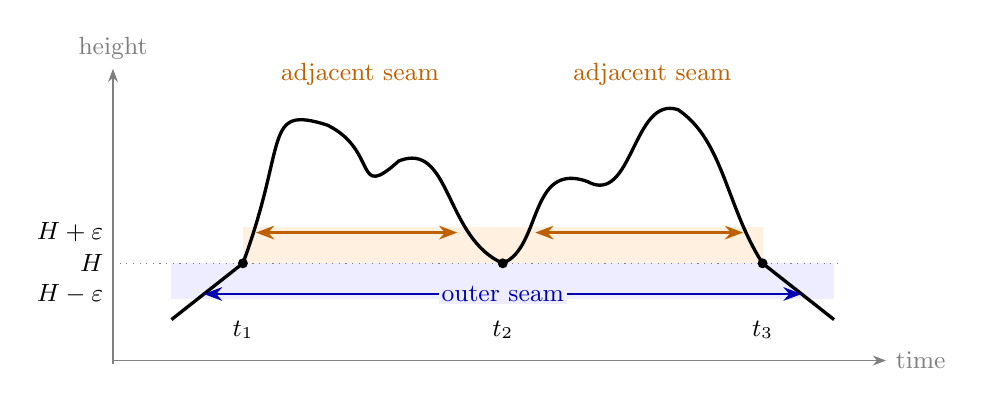
\begin{tikzpicture}[x=1.65cm,y=1.3cm,>=Stealth,font=\small]
  \fill[blue!7] (0.45,-0.35) rectangle (5.55,0);
  \fill[orange!12] (1,0) rectangle (3,0.35);
  \fill[orange!12] (3,0) rectangle (5,0.35);
  \draw[->,gray] (0,-0.98)--(0,1.9) node[above]{height};
  \draw[->,gray] (0,-0.95)--(5.95,-0.95) node[right]{time};
  \draw[gray,dotted] (0,0)--(5.6,0);
  \node[left] at (0,0) {$H$};
  \node[left] at (0,-0.3) {$H-\varepsilon$};
  \node[left] at (0,0.3) {$H+\varepsilon$};
  \draw[very thick] (0.45,-0.55)--(1,0)
    .. controls (1.35,1.2) and (1.15,1.55) .. (1.65,1.35)
    .. controls (2.05,1.1) and (1.85,0.6) .. (2.2,1.0)
    .. controls (2.6,1.2) and (2.55,0.25) .. (3,0)
    .. controls (3.3,0.15) and (3.2,1.0) .. (3.65,0.8)
    .. controls (4.0,0.55) and (4.0,1.65) .. (4.35,1.5)
    .. controls (4.7,1.2) and (4.72,0.55) .. (5,0)
    --(5.55,-0.55);
  \draw[blue!70!black,thick,<->] (0.7,-0.3)--(5.3,-0.3);
  \node[blue!70!black,fill=blue!7,inner sep=1pt] at (3,-0.3)
    {outer seam};
  \draw[orange!75!black,thick,<->] (1.1,0.3)--(2.65,0.3);
  \draw[orange!75!black,thick,<->] (3.25,0.3)--(4.85,0.3);
  \node[orange!75!black] at (1.9,1.85) {adjacent seam};
  \node[orange!75!black] at (4.15,1.85) {adjacent seam};
  \foreach \x/\i in {1/1,3/2,5/3}{
    \fill (\x,0) circle (1.8pt);
    \node[fill=white,inner sep=1pt] at (\x,-0.65) {$t_\i$};
  }
\end{tikzpicture}
\caption{A triple contact in one contour coordinate. The visits
$t_1<t_2<t_3$ at height $H$ represent the same surface point.
Overlaps below $H$ join the outer visits; overlaps above $H$ join
adjacent visits. Their directions determine the relative offsets and
identify the middle run, whose exact minimum supplies the cutoff $H$.
Omitted gaps stay separated from the retained bands by a positive
height margin. This diagram shows the incidences schematically.}
\label{tree:fig:triple-contact}
\end{figure}


The same configuration explains a lower endpoint that must not be
discarded.  A seam between an outer run and the middle run begins
at $H=m_w^a+s_w^a$ and has positive length above $H$.  Choose its
rational band to extend below $H$.  The exact incoming or outgoing
record condition in the middle run clips it at the discrete minimum
$s_{w,n}^a+m_{w,n}^a$.  Hence links at that minimum, as well as links
at lattice heights converging to it from above, are retained.  No
new comparison with an omitted gap is introduced.  Positivity of
the shared interval above $H$ already provides slack from every
upper cutoff.  More generally the lower endpoint of a shared seam
is the larger of its two natural record-arc minima, by
Equation~\eqref{tree:eq:gap_minimum_condition}; these exact natural
conditions handle it in precisely the same way.  Thus neither
lower endpoints nor upper branch cutoffs require an additional
joining cost for each crossing.

For each coordinate, join run vertices whenever such a positive
overlap is used and retain a spanning forest of this graph.  Differences
along the forest recover all offsets needed by its bands and caps.
Cycles require no additional random parameters: their sums are zero
because they are differences of the same height coordinates.  An
isolated component requires no absolute height and no comparison with
another component.  In particular there is no need to infer the
chronological ordering of two remote runs without a shared seam.
The direction of a declared seam specifies the order of its two ends;
the three directed overlaps specify an intermediate cap.  The omitted
chronological ordering is used only in the proof that the local
instructions are valid, and is not an input to them.

\emph{A finite family of whole bands.}
There are finitely many run pairs and gap pieces. For each relevant
pair, its height set is compact.  Cover it by bands with rational
endpoints lying in positive seam overlaps, allowing rational lower
endpoints below a natural minimum and clipping by the exact record-arc
condition as just explained.  Use the exact selected-minimum cap when
an upper overlap endpoint belongs to the height set.
The preceding positive-overlap and omitted-gap arguments supply a
neighborhood of every height, so a finite subcover exists.  Include
the finitely many additional overlaps used to recover the offset
forest.  This produces one finite instruction list.  Each instruction
retains \emph{all} discrete links in its band; it does not prescribe
one crossing of that band.  Consequently the same list captures paths
with an arbitrary, even diverging, number of crossings.

Uniform contour convergence now proves capture.  If a discrete link
near $K$ failed to be captured infinitely often, a limiting endpoint
pair would belong to the compact set just covered.  In its selected
band, outgoing and incoming record conditions are the original
discrete conditions, all selected minima are tested exactly, and
omitted gaps have a fixed positive slack.  The link therefore satisfies
the instruction for all sufficiently large resolutions, a contradiction.
Internal tree steps and internal matches are already included.

\emph{Realization and refinement.}
For realization, consider an admissible chart and a compactly confined
limiting path.  On a band strictly interior to a genuine shared seam,
Equation~\eqref{tree:eq:gap_minimum_condition} has positive margin from
every omitted obstruction.  At a cap the local three-overlap test
identifies the selected intermediate minimum; its exact discrete
comparison supplies the only possibly non-strict condition.  The
remaining omitted obstructions have positive slack on the confined
compact set, by the same minimum argument.  Thus each permitted link
of the discrete approximants is an actual link once the resolution
is sufficiently large.  This conclusion is uniform over all their
links, because there are finitely many bands and the slack is uniform.
If endpoint representatives differ, the joining conclusion of
Proposition~\ref{tree:prop:certificate_limit} corrects them in an arbitrary
open margin at vanishing cost.

A refinement retains all old cut anchors and active windows and adds
cuts.  An old active window remains the same whole cut-to-cut interval;
its internally enabled edge set is not changed by the extra cuts.
When master strings are merged, the old windows remain selectors in
the merged string, their starting heights are calculated from its
increments, and their band anchors retain their exact values.  Each
old test graph is therefore \emph{calculated directly} from the merged
input using its old edge-witness windows and band list.  It is retained
as its own output component, alongside any new graph enabled on the
larger union.  It is not recovered by restricting ranges of paths in
the larger graph, which could use newly enabled gap edges.  Additional
arc or minimum windows may be subdivided using the finite selector
language without changing the old active internal windows.  Thus
every old path and every ordered marking remains exactly an output
of its old test.  Countably many
such operations were included in the extraction.  Applying capture
and realization with margins decreasing to zero proves the third
assertion.  Measurability follows by using the countable instruction
lists and rational positive margins in the local tests above.

Finally, if $K$ is compactly in the interior of an interval cell
$\eta([a,b])$, all its curve-time preimages lie in $(a,b)$.  Indeed
interval interiors are disjoint from the images of disjoint time
intervals; this is also a consequence of the area parametrization
and the disk-cell property of Theorem~\ref{tree:thm:background_peanosphere}.
Compactness makes the containment uniform.  All cells selected near
$K$ are then internal to $[a,b]$, so the entire construction uses only
links witnessed in that interval.
\end{proof}

\subsection{Conditional transfer from independent intervals}

The finite graph tests use local data, but their limiting conditional
laws still need to be identified. We compare independent input blocks
with the same blocks in the full walk. Poissonizing the jump clock
removes lattice parity; the following lemma controls the interval
endpoints when we return to the original clock.

\begin{lemma}[Stability at nonidentified cuts]\label{tree:lem:cut_stability}
Suppose two pairs of discrete time endpoints converge to the same
$a<b$ in a common bounded contour window, and the Brownian fibers
of $a$ and $b$ are singletons.  Under the uniform internal time
modulus of Lemma~\ref{tree:lem:moment_compactness}, their internal
endpoint distances, in the common cost units, differ by
$o_{\Prob}(1)$.  If their $k$th powers are uniformly integrable,
their $k$th moments have the same limit.  This applies simultaneously
to every fixed finite set of deterministic or independent Poisson cuts.
\end{lemma}

\begin{proof}
It suffices to compare the smaller and larger intervals formed from
the two pairs of endpoints.  The added portions are shrinking time
fringes near $a$ and $b$.  Every edge available in the larger internal
graph but not the smaller one has a witnessing step or match endpoint
in one of these fringes.  Likewise an old vertex represented in an
added fringe is linked by a first-coordinate identification to that
representative.  Uniform contour convergence and singleton fibers
imply that all these incidences and their other representatives lie
in time neighborhoods of the same cut whose radii tend to zero in
probability.  Indeed, otherwise a subsequence in the containing
compact window would give a link with one limiting endpoint $a$
or $b$ and its other endpoint a different time, contrary to the
singleton assumption.  The two neighborhoods are disjoint eventually.

Take a path in the larger graph between its tips.  Every newly
available edge is confined to one of these two neighborhoods.  Keep
the part after the last visit to the left neighborhood before the
first visit to the right neighborhood.  Its middle uses only edges
of the smaller graph.  Its first and last old vertices have smaller
interval representatives in the respective shrinking cut neighborhoods.
Connect them internally to the smaller interval's tips using the
time modulus.  This adds $o_{\Prob}(1)$ once at each end.  It does
not pay separately for the possibly many discarded fringe visits.
Taking infima bounds the smaller interval's endpoint cost by the
larger one's plus this error.  Graph inclusion and short endpoint
pieces in the larger interval give the reverse inequality.  The
moment assertion follows from uniform integrability.  Fixed and
independent Poisson times have singleton fibers almost surely by
the Brownian facts used in Proposition~\ref{tree:prop:certificate_limit},
so conditioning on their countable collection proves the last claim.
\end{proof}

Put the bilateral axial walk on an independent Poisson jump clock of
rate $n$ in macroscopic time.
The coordinate walks are then independent continuous-time simple walks,
each of variance rate $\sigma^2=1/2$ before diffusive rescaling.  We write
$\epsilon_n=n^{-1/2}$ and use rescaled heights in
$\epsilon_n\Z$.  This removes parity constraints.  The clock satisfies
the uniform law of large numbers on each bounded time interval.
Replacing every jump time by its jump index is an \emph{exact}
relabeling of the full sewn graph.  A formal test cut at clock time
$T$ becomes a cut at index time $J_n(T)/n$; its active edge-witness
windows, oriented step incidences, height anchors, and costs are
identical.  The law of large numbers says only that these relabeled
cuts have the same limiting marks.  We do not infer continuity of
arbitrary formal test outputs under independently moved cuts.
For internal endpoint norms with fixed macroscopic endpoints,
Lemma~\ref{tree:lem:cut_stability} supplies the additional comparison.
The moment argument of Lemma~\ref{tree:lem:moment_ui} also applies in
Poisson time: disjoint clock intervals have independent strings,
their step counts concentrate, and the probability of a count
outside a fixed multiple of its mean decays exponentially.  The
trivial cost bound by the count controls this last event.  Thus
the same mixed-monomial argument gives uniform integrability, and
the cut-stability lemma transfers the internal $k$th moments as
well.  This justifies returning to fixed walk lengths.

\begin{lemma}[Finite reference experiment and conditional transfer]
\label{tree:lem:finite_kernel_transfer}
Fix finitely many chart packages.  A package may contain several
overlapping instruction tests; tests in different packages use disjoint
blocks and disjoint offset forests.  Give the block durations and
relative internal cuts a smooth positive density on their ordered
parameter domain.  Sample independent Poissonized increment strings
on the blocks. Independently, sample the forest offsets with smooth
positive probability densities, assigning each point of
$\epsilon_n\Z$ the density's mass in its centered half-open lattice
cell. Retain the complete
marked certificate data of the package's canonical instruction graphs.

There is a common subsequence on which these reference experiments,
for all finite packages in the countable instruction language, have
conditional limiting kernels
\begin{equation}\label{tree:eq:reference_kernel}
 \nu_r(dx_r)\,K_r(x_r,dy_r).
\end{equation}
Here $x_r$ consists exactly of the relative block durations, internal
cuts, increment paths, and forest offsets, and $y_r$ is the package's
additional certificate data.  The following statements hold.
\begin{enumerate}
\item Insert the selected blocks, in any chronological order consistent
with the desired actual word, with positive-duration omitted gaps.
Then in the limiting actual-walk experiment, conditional on the
\emph{entire} limiting contour and all cut marks, the law of the
additional package data is $\bigotimes_r K_r(x_r,\cdot)$.
\item The kernel is independent of absolute time locations, integer
cut labels, and the chronological ordering of pairs of blocks not
used by the instruction list.  It is unchanged by replacing the
smooth positive reference densities.  Relabeling blocks or replacing
an offset forest by another basis for the same differences transforms
the kernel by the corresponding deterministic relabeling of its inputs
and outputs.
\item These assertions hold jointly for finite collections of tests,
with their common refinements, and remain true after measurable
selection from the jointly retained countable family of instruction
templates and finite cut-mark lists. The selection may depend on the
limiting contour and marks. Selection is
performed after conditioning; no claim of this kind is made for
selection based on the additional passage data.
\end{enumerate}
\end{lemma}

\begin{proof}
We compute the density of the actual block offsets, insert the omitted
intervals as bridges, and then condition on the whole contour. We finish
by checking relabeling and refinement, which are needed for local chart
selection.

\emph{Independent reference experiments.} Under the
reference law, distinct packages are independent. Their input
marginals converge by the invariance principle and lattice
approximation of the offsets: sample a real offset from its density
and replace it by the center of its lattice cell, moving it by at most
$\epsilon_n/2$. Their output coordinates belong to
compact hyperspaces, so after extraction the joint laws converge to
Equation~\eqref{tree:eq:reference_kernel}.  The joint limit of independently
sampled packages is their product; this statement concerns joint weak
convergence, and imposes no regularity on the conditional kernels $K_r$.

\emph{The exact change of density.}
First treat one coordinate and fix the continuous cut parameters.
List all selected blocks in their actual chronological order
$1,\ldots,m$.  Let $s_i$ be their starting heights, $e_i$ their net
increments, and $g_i>0$ the gap duration from the end of block $i$ to
the beginning of block $i+1$.  Set $s_1=0$, since all graphs are
invariant under a common height translation.  Complete the union of
the package forests to a tree $T$ on the $m$ blocks.  Add independent
offset variables on its extra edges, with positive smooth densities.
For an edge $e$ with smooth positive probability density $\rho_e$,
its discretized mass is
\begin{equation}\label{tree:eq:offset_mass}
 r_{n,e}(a)=\int_{a-\epsilon_n/2}^{a+\epsilon_n/2}\rho_e(u)\,du,
 \quad a\in\epsilon_n\Z.
\end{equation}
The half-open cells partition $\R$, so these positive masses sum
exactly to one. Uniform continuity on compact sets gives
$\epsilon_n^{-1}r_{n,e}(a)\to\rho_e(a)$ uniformly for $a$ in a compact
set. Gaussian densities are one possible fixed choice; the construction
applies to every smooth positive probability density.

The map from the $m-1$ tree differences to
$(s_2-s_1,\ldots,s_m-s_{m-1})$ is unimodular.  To prove this, recover
each $s_i$ by summing signed edge differences along the unique path
in $T$ from $1$ to $i$.  This is an integer linear map.  Its inverse
is obtained by reconstructing the $s_i$ from the consecutive differences
and subtracting the appropriate two values for every tree edge.
Both maps have integer entries, so their determinants are integers
whose product is one.  Thus their determinants are $+1$ or $-1$,
and no extra lattice multiplicity occurs.

Let $p_t(k)$ be the transition mass of the unscaled coordinate walk
in time $t$.  Conditional on the selected block paths, the required
gap displacement is
$\epsilon_n^{-1}(s_{i+1}-s_i-e_i)$.  The exact density of the actual
relative starts with respect to the reference offset law is
\begin{equation}\label{tree:eq:forest_density}
 W_n^{a}=
 \frac{\displaystyle\prod_{i=1}^{m-1}
   p_{ng_i}\bigl(\epsilon_n^{-1}(s_{i+1}-s_i-e_i)\bigr)}
 {\displaystyle\prod_{e\in T}r_{n,e}(a_e)}.
\end{equation}
Indeed, summing its numerator over all consecutive gap displacements
gives one, and unimodularity identifies this sum with the sum over
tree offsets.  Multiply Equation~\eqref{tree:eq:forest_density} for the
two coordinates and multiply by the ratio of cut-parameter densities.
This is the full density $W_n$.  If an absolute starting value is
needed for reconstructing the whole contour, include an anchored
additional block, or record that value separately; no chart graph
uses it.  External past and future portions are added conditionally
on the extreme endpoints in the same way as the gaps.

\emph{Uniform density and bridge limits.}
The Fourier formula for a continuous-time coordinate walk is
\begin{equation}\label{tree:eq:poisson_walk_fourier}
 p_{nt}(k)=\frac1{2\pi}\int_{-\pi}^{\pi}
 \exp\{-n\sigma^2t(1-\cos\theta)-ik\theta\}\,d\theta.
\end{equation}
After $\theta=\epsilon_n u$, the integrand converges to
$\exp\{-\sigma^2tu^2/2-ixu\}$ when
$\epsilon_n k\to x$.  The bound
$1-\cos\theta\geq2\theta^2/\pi^2$ for $|\theta|\leq\pi$
gives an integrable Gaussian majorant uniformly when
$t\in[t_-,t_+]\subset(0,\infty)$.  Truncating the $u$ integral
first also gives uniformity in $x$ on compact sets.  Therefore
\begin{equation}\label{tree:eq:uniform_gap_lclt}
 \sup_{\substack{t\in[t_-,t_+]\\ |\epsilon_n k|\leq M}}
 \left|\epsilon_n^{-1}p_{nt}(k)-
 \frac{e^{-(\epsilon_n k)^2/(2\sigma^2t)}}
 {\sqrt{2\pi\sigma^2t}}\right|\longrightarrow0.
\end{equation}
There are $m-1$ numerator and denominator lattice factors in
Equation~\eqref{tree:eq:forest_density}; they cancel.  On compact parameter
sets with positive gap durations, $W_n$ thus converges uniformly to
a finite positive continuous function $W$.

Conditional on the selected block paths and their starts, the omitted
gaps are independent bridges and are independent of every $y_r$.
Their rescaled laws converge uniformly, on the same compact parameter
sets, to the corresponding Brownian bridges.  Here is a proof of the
uniform assertion.  Their finite-dimensional densities are products
of the transition masses divided by the whole-gap mass; applying
Equation~\eqref{tree:eq:uniform_gap_lclt} proves convergence at times
bounded away from each other and the endpoints.  On the first half
of a gap of duration $t$, the bridge density with respect to the
unconditioned walk started at its first endpoint is
\[
 \frac{p_{n(t-u)}(k-X_{nu})}{p_{nt}(k)},\qquad u\leq t/2.
\]
The denominator is at least $c\epsilon_n$ for compact endpoint
displacements and $t\in[t_-,t_+]$.  The Fourier bound gives a numerator
at most $C\epsilon_n$ uniformly in its integer argument.  Thus the
density is uniformly bounded.  The free-walk invariance principle
gives tightness on this half.  Time reversal proves it on the second
half.  Together they prove bridge tightness; the finite-dimensional
limits identify every subsequential limit, proving uniform convergence.
The same argument applies to a finite vector of gaps and to external
contour pieces on any bounded window.

\emph{Conditioning on the complete contour.}
Let $a$ denote the added completion offsets and let $z$ denote all
omitted bridge paths.  Test the joint law against products of bounded
continuous functions of the inputs, outputs, and bridges.  Integrate
the bridge variables first.  On a compact parameter set, uniform
bridge convergence replaces the bridge conditional expectation by
its Brownian counterpart, and uniform convergence of $W_n$ replaces
the density by $W$.  Product convergence of the independent reference
packages then gives the limiting law
\begin{equation}\label{tree:eq:full_contour_kernel_factor}
 W(x,a)\,\nu(dx,da)\,\mathcal B(x,a;dz)
       \prod_r K_r(x_r,dy_r).
\end{equation}
The factor $W$ need not factor across packages.  Both it and the
bridge law $\mathcal B$ depend only on the contour inputs, not on
the additional passage variables.  The complete contour and its
cut marks recover $(x,a,z)$, including the unused completion offsets.
Disintegration of Equation~\eqref{tree:eq:full_contour_kernel_factor}
therefore leaves exactly $\prod_rK_r(x_r,dy_r)$.

We remove the compact restrictions explicitly.  Exhaust the finite
cut-parameter domain by compact sets on which gap durations are
positive, then bound endpoints and offsets, and finally bound the
selected block paths in compact sets of the continuous-path topology.
Under the actual law these exclusions have probability tending to
zero, uniformly along the sequence, by the finite-block invariance
principle, tightness, and positivity of the finitely many limiting
cut gaps.  If $Q_n$ is the reference law and $P_n$ the actual law,
\[
 \E_{Q_n}[W_n\mathbf1_{A^c}]=P_n(A^c).
\]
Thus the same exhaustion controls the discarded density mass.
On each compact set the densities were uniformly bounded.  This
justifies the limiting density calculation and its normalization;
it does not assume a global bound for $W_n$.  A monotone-class
argument now gives the conditional identity for bounded measurable
tests.  Increasing bounded contour windows gives conditioning on
the entire bilateral contour.

\emph{Labels, reference densities, and overlapping tests.}
Before any limiting operation, the canonical graph map
restarts each block's clock at zero and its increments at zero.  Its
only noninternal numerical inputs are the specified forest differences.
It never uses the original integer cut index, an absolute starting
height, the starting time of a block, or any omitted jump count.
The global chronological permutation appears only in
Equation~\eqref{tree:eq:forest_density}.  Since this weight disappears
from the conditional output law in
Equation~\eqref{tree:eq:full_contour_kernel_factor}, that permutation is
not an additional parameter of $K_r$.

Changing a smooth positive reference density multiplies the joint
reference law by a function of the input variables alone. On a
compact parameter set the ratio of the lattice cell masses converges
uniformly to the continuous density ratio. The preceding test-function
argument, without bridge variables, therefore leaves the limiting
kernel $K_r$ unchanged. Exhaustion is justified under the replacement
law by tightness of the lattice approximations. The same argument
allows any smooth positive joint density for the finite forest-offset
vector within a package, independent of its strings: integrate over
the product lattice cells and use their common volume. Distinct
packages remain independent.

A permutation of block names is an exact relabeling of the finite
graph map. A change of forest basis is a unimodular integer linear
map $U$ of the offset vector, and recovering the same height
differences gives exactly the same graph. To compare the discretized
input laws, write $C=[-1/2,1/2)^d$ for the unit cell in this vector
space. The pushed-forward masses integrate the transformed smooth
joint density over cells $b+\epsilon_n UC$; its direct discretization
uses $b+\epsilon_n C$. Both cells have volume $\epsilon_n^d$ and
diameter tending to zero. Their masses divided by this volume
converge uniformly on compact sets to the same positive density.
Thus the ratios of the two masses tend uniformly to one there.
Both lattice laws are tight, as each is a vanishing displacement
of the same continuous input law, so their total variation distance
tends to zero. Applying the graph map preserves this bound even
when its output is discontinuous. Density invariance now identifies
the new-basis kernel with the transformed old kernel. This also
allows different positive reference densities for different finite
tests. Consequently a locally measurable enumeration of blocks
leaves no global label in the kernel.

For overlapping tests retain their joint output in one package and
apply the preceding argument to the union of their finite graphs.
The independently sampled blocks in this common experiment are always
the maximal consecutive runs of the union.  Adjacent pieces inside
one such run are recorded subwindows of a single block, with their
relative starts determined by that block's increments.  They are
never treated as separate independent blocks with a zero-duration
gap or a smooth density on their forced offset.  Thus all gaps to
which Equation~\eqref{tree:eq:forest_density} is applied remain positive.
If two forest choices are required, express their union of differences
in a single spanning forest, as above.  For disjoint spatial packages,
the block sets and their forests are disjoint, so their union is a
forest and the same completion calculation applies, even if their
chronological runs interleave.

\emph{Merging master blocks.}
If previously omitted
gaps are included, old separate strings can become windows in a new
master string.  Their offsets are then functions of that master
string; it would be invalid to restrict an arbitrary version of an
old kernel to this forced-offset relation.  Instead, start with the
old independent strings, smooth forest offsets, and their old test
outputs.  Insert the positive-duration old gaps as conditional bridge
strings and multiply by the exact density
Equation~\eqref{tree:eq:forest_density}.  The resulting concatenated string
has exactly the law of the new master string.  The old output is
unchanged, since its active edge-witness windows and band list are
unchanged.  Calculate any new union graph as an additional output
component on this same master string.  Applying the already-proved
density and bridge convergence to the old output gives precisely
Equation~\eqref{tree:eq:full_contour_kernel_factor}; hence its conditional
law given the entire new master contour is its original $K_r$.
This identity is proved before conditioning the master path, when
the gap endpoint differences have their ordinary densities.  There
is no conditioning of a preexisting almost-everywhere formula on a
singular slice.  If an old gap has duration zero, it was already
within a single old master block and the active-window identity is
exact without a density change.  For several old tests retain their
whole vector of outputs, together with the new test, before the
same operation.  Thus joint outputs, rather than filtered paths of
a larger graph, prove common-refinement compatibility.
We do not assert that a new union output is independent of the newly
observed bridge strings.  The calculation of the old conditional
marginal first integrates out that new output; the full output
vector is retained separately in the master experiment.

Extracting the countably many finite packages jointly preserves
these identities by the same compact density and bridge argument.  After
conditioning on the full contour and cuts they hold simultaneously
outside one null set, and hence also for a countably valued
contour-measurable selection.  This proves the lemma.
\end{proof}

\begin{proposition}[Spatial product kernels]\label{tree:prop:locality}
For every open coordinate domain $U$, the collection of all certificates
with compact range in $U$ has a regular conditional law
$\mathsf K_U(h|_U,\widehat h|_U;\cdot)$ depending only on the restrictions
of the two fields to $U$.  If $U_1,\ldots,U_m$ are disjoint open sets,
these collections are conditionally independent given the complete
fields, with respective conditional laws $\mathsf K_{U_i}$.
These laws are consistent under restriction and exhaustion.  They
also exist on the free-field patches obtained by local absolute
continuity in Proposition~\ref{tree:prop:background_locality}.
Here the local collection retains projected endpoints and ranges,
costs, and ordered-subpath incidences; the original global contour-time
labels have been forgotten.  Relative parametrizations inside locally
retained cells may be used during the construction.

In particular one can preserve a sampled collection on each of finitely
many disjoint patches and complete it to a sample of the whole
certificate law, provided that the preserved collections have the
specified product conditional law for the new fields on those patches.
This statement concerns conditional sampling; it makes no assertion
that the competitor satisfies a Weyl rule.
\end{proposition}

\begin{proof}
\emph{Finite charts with marks retained.}
Fix finitely many buffered charts in
each of the disjoint sets.  Refine and merge their instructions within
each set.  Different sets use disjoint cells.  Maximal runs from
different sets cannot share a cut: the shared point would belong to
both compactly contained cells.  Thus their distinct runs have
positive intervening time gaps.  Lemma~\ref{tree:lem:finite_kernel_transfer}
applies to these packages.

The reference kernel in that lemma has four kinds of input: relative
area durations, increment functions, internal relative cuts, and
forest height differences.  Lemma~\ref{tree:lem:chart_reconstruction}
reads all four from the oriented cells and boundary lengths in the
given patch.  The same local data give the embedding map that sends
the time-labelled ranges in the reference output to spatial ranges.
The conditional output law, after that map, is therefore a function
of the fields and marks \emph{in that patch}.  Lemma~\ref{tree:lem:finite_kernel_transfer}
also proved invariance under global block labels, reference densities,
and forest bases.  Thus replacing global cut indices by a local
enumeration of the cells does not discard a parameter on which the
kernel might still depend.  This explicit invariance is necessary;
conditional factorization given extra global labels would not by
itself prove the present assertion.

\emph{Conditioning on the fields.}
Realize the continuum fields by sampling their regular
conditional law given the peanosphere contour, independently of the
additional raw, time-labelled reference outputs and all time cuts
conditionally on that
contour.  This
is simply the prescribed mating-of-trees coupling, with any residual
embedding or imaginary-field randomness supplied at this stage.
Consequently the product identity from
Equation~\eqref{tree:eq:full_contour_kernel_factor} remains true on
conditioning additionally on these fields.  Its right-hand side
has just been shown measurable in the local fields and local marks.
Taking conditional expectation with respect to the complete fields
and marks gives the same product identity.  No determination of the
additional passage data by the continuum fields was used.

\emph{Exhaustion.}
Enumerate the countable instruction templates and
their rational positive-margin tests.  Within a patch, enumerate the
locally retained cells and all finite selections from them, using any
fixed measurable ordering of their embedded marked points.  Every
finite set of these tests has the conditional law just proved, with
the consistency supplied by the common-refinement part of
Lemma~\ref{tree:lem:finite_kernel_transfer}.  Hence they define a conditional
law on the countable product of compact certificate spaces.  Cylinder
events form a determining algebra.  The capture and realization
parts of Lemma~\ref{tree:lem:chart_reconstruction}, followed by an
exhaustion $K_j\Subset U$, identify the measurable collection generated
by this algebra with the local projected part of the original retained
array $\mathcal H$.  More explicitly, $\mathcal H_n$ and all the
charts were calculated from the same word and were extracted jointly.
Capture puts every compactly confined element of its limit in the
chart exhaustion; realization gives the reverse inclusion.  Both
statements include every finite number of ordered marks.  Thus no
new coupling between a metric and Poisson marks is chosen at the
limit.  The time cuts remain independent of the original array
and background, since their finite-resolution joint law was a
product and they were retained jointly.
They also identify the restriction maps for nested domains.  The
finite product identities on cylinder events extend by a monotone
class to the full local collections and then to countably many
subdomains when needed.

\emph{Removing the marks.}
Conditional on $(h,\widehat h,\eta,\mathcal H)$, the time cuts are still the
independent Poisson processes used at the start.  Since
$\eta_*(dt)=\mu_h$, the Poisson mapping theorem shows that the spatial
marks have their prescribed intensities proportional to $\mu_h$.
Their law consequently has that same form conditional on both fields,
and their restrictions to disjoint sets are independent under this
conditioning.  Nested refinements are obtained by independent
local superposition.  Integrating the marks out of the preceding
conditional product law therefore gives
\[
 \bigotimes_i\left(\int
  \mathsf K_{U_i}^{\mathrm{marks}}(h|_{U_i},\widehat h|_{U_i},\pi_i;\cdot)
     \,\operatorname{Pois}_{h|_{U_i}}(d\pi_i)\right).
\]
The factor in parentheses defines $\mathsf K_{U_i}$.  This proves
fields-only dependence and factorization, rather than merely a
mark-conditioned assertion.

\emph{Field changes and completion.}
On a relatively compact patch, change the field marginal by a locally
absolutely continuous density and retain the same conditional kernel.
The identities are preserved because the density is a function of
the conditioning variables.  Two such constructions agree on their
overlap by mutual absolute continuity and the established restriction
consistency.  An exhaustion yields the stated free-field versions.
All spaces used are standard Borel, so regular conditional laws exist.
Disintegrate the whole law over its restrictions to the preserved
patches to obtain the completion assertion.  If a recipe is subsequently
selected using the full sampled configuration, restriction to the
selection event gives a submeasure of this unrestricted construction;
it does not require a new conditional-independence claim.
\end{proof}

\subsection{Open margins, nondegeneracy, and changes of units}

The local kernels are now constructed. We next record the properties
needed when the laws themselves vary: inequalities pass through open
margins, the augmented construction survives further limits, and a
positive internal norm prevents all local costs from vanishing.

\begin{lemma}[Buffered tests]\label{tree:lem:certificate_buffered_tests}
Consider a convergent sequence in the certificate topology with a
uniform interval modulus.  Fix $K\Subset U$, a finite cost cutoff,
and compact endpoint sets in $K$.  The following implications hold.
\begin{enumerate}
\item An upper connection bound in the limit with a strict cost
margin and with certificates compactly in $U$ implies the same bound,
with a smaller margin, for the approximants.  Uniform bounds over
compact endpoint sets follow from finitely many witnesses and the
joining modulus.
\item A sequence of paths in $K$ violating a fixed lower traversal
bound, with bounded costs and endpoints in prescribed closed sets,
has a limiting certificate violating the corresponding weak bound
in $U$.  Any finite list of ordered crossings or subpaths can be
retained with it.
\item Suppose reference metrics $D_n$ are retained in the joint
topology and converge locally uniformly to a continuous length
metric $D$ inducing the ordinary topology.  Local inequalities
$F_n\leq C_nD_n$ along reference geodesics in arbitrary open margins,
and lower bounds on all certificates by $c_nD_n$, pass to the limit
when $C_n\to C<\infty$ and $c_n\to c\geq0$.
\end{enumerate}
These implications also hold under any fixed absolutely continuous
change of the retained continuum marginal.
\end{lemma}

\begin{proof}
For the first assertion, start with one limiting certificate.  Its
range has a positive distance from $U^c$, and its cost is strictly
below the bound, so its approximants retain both margins.  For a
compact endpoint family, continuity and uniform joining provide
neighborhoods of the endpoints in which one may use this certificate
with a prescribed small additional cost.  Finitely many such
neighborhoods suffice.  This gives the uniform finite-net assertion,
with no claim at $\partial U$.

For the second assertion, mark the specified crossing endpoints
before extraction.  Proposition~\ref{tree:prop:certificate_limit} gives
a converging marked certificate subsequence.  Closed endpoint
constraints and non-strict cost upper bounds persist in this
subsequence; its range is in $K\Subset U$.  This proves the required
contrapositive of the lower-bound transfer.

For the upper part of the third assertion, take a $D$-geodesic with
range compactly in an open margin.  Partition it into sufficiently
short segments.  The partition is finite.  For each segment,
continuity of $D$ and positive $D$-distance from its small surrounding
neighborhood to that neighborhood's outer boundary imply that a
$D_n$-geodesic between its endpoints stays in this neighborhood for
all sufficiently large $n$.  To justify existence and containment
one may work in a larger compact length-space chart: a competitor
of sufficiently small $D_n$-length beats every path reaching the
outer boundary, whose endpoint distance is bounded below by local
uniform convergence.  The sum of these $D_n$-distances converges to
the sum of the corresponding $D$-distances, which is the length of
the original geodesic.  Apply the assumed upper comparison on each
piece, concatenate, and extract.  The lower comparison follows
directly by applying it to approximants of a limiting certificate.
For a fixed change of marginal density $w$, approximate $w$ in
$L^1$ by bounded continuous functions of the retained continuum
data.  The convergence assertions pass for each such approximation,
and the $L^1$ error bounds the discarded probabilities uniformly.
\end{proof}

\begin{lemma}[Closure under further limits]\label{tree:lem:certificate_class_closed}
Augment a continuum certificate law by its original raw, time-labelled
array $\mathcal H$ and its projected local arrays as separate coordinates,
the common fixed continuum background, the independent
time cuts, and the laws of all finite independent reference packages
in Lemma~\ref{tree:lem:finite_kernel_transfer}.  The packages retain all
active-window tests, old and new outputs under master-block merging,
and the countably many fixed unit transforms.  Their continuum input
marginals are the fixed reference marginals $\nu_r$ in that lemma.
Suppose a sequence of such augmented laws has a common interval
modulus and the internal moment uniform integrability above.  Every
joint weak subsequential limit of these augmented data has the same
certificate, reference-transfer, reconstruction, and spatial
product-kernel properties.  In particular this class is closed
under the varying-law and varying-zoom extractions used below.
\end{lemma}

\begin{proof}
The input marginals of the reference experiments are fixed. This lets
us pass their density identities to a new limit, then recover the local
spatial collections from the retained raw arrays.

Write the $r$th reference law at stage $j$ as
$\nu_r(dx_r)K_{j,r}(x_r,dy_r)$.  The output spaces are compact,
the variables $y_r$ are the raw time-labelled outputs, and the input
marginals are fixed.  After joint extraction these
laws converge to $\nu_r(dx_r)K_r(x_r,dy_r)$.  For independent
packages, their product laws converge to the product of these
limits.  This is a statement about independent full experiments,
not a claim that arbitrary conditional independence is weakly closed.

For a fixed finite family, first restrict to compact input parameters
with positive gap durations.  The density $W$ and Brownian bridge
law in Equation~\eqref{tree:eq:full_contour_kernel_factor} are now the
same for every $j$.  On this compact set $W$ is bounded and
continuous; the bridge law is weakly continuous in the endpoints
and positive durations, by the bridge argument in
Lemma~\ref{tree:lem:finite_kernel_transfer}.  Integrating bounded
continuous bridge tests therefore preserves joint weak convergence
of the reference packages.  Hence that equation holds with the
new $K_r$.  The error in removing the compact restrictions is the
probability of the excluded parameters under the actual contour
law.  This law is fixed and does not depend on $j$ or on the
additional passage kernels.  Its exhaustion error tends uniformly
to zero.  Thus the full-contour factorization, label removal, and
forest-basis invariance all pass to the limit.

For merging, retain the entire vector of old and new test outputs
in the master experiment.  The old component is obtained at finite
resolution using the same active edge-witness windows.  The
positive-gap density-and-bridge construction near the end of
Lemma~\ref{tree:lem:finite_kernel_transfer} proves its conditional
marginal identity under observation of the new master string.
That construction uses the same continuous $W$ and bridge law,
so its identity passes by the preceding argument.  The output
coordinates and their deletion-of-marks maps are continuous maps
on the retained compact arrays.  Joint consistency of every
finite group of tests is consequently preserved.  No conclusion
is obtained by restricting a merged distance or by evaluating an
old kernel on a forced-offset diagonal.

First pass the fixed conditional coupling of the additional continuum
background with the contour, using only raw output tests.  For a
bounded background test, approximate its conditional expectation
given the contour by bounded continuous functions in $L^1$ of the
fixed contour marginal.  Multiplication by a bounded test of the
raw $\mathcal H$ or raw reference outputs keeps the error uniform
over $j$.  Joint weak convergence then preserves this conditional
sampling identity.  This argument is applied before projection;
projected outputs also depend on the background and are not claimed
conditionally independent of it.  It explains why the common full
background and its unit transforms must be retained, as in
Section~\ref{tree:sec:coherent-background}, rather than sampled separately at
successive scales.

Now project raw endpoints and ranges through the retained curve.
On each bounded time window, $(\eta,K)\mapsto\eta(K)$ is continuous
for uniform convergence of the curve and Hausdorff convergence of
the compact range; the same holds for every finite list of marks.
Thus the raw arrays and background determine their joint projected
limits.  The projected local part of the original $\mathcal H$
agrees with the chart exhaustion, with open margins:
on each compact $K\Subset U$, the proof of
Lemma~\ref{tree:lem:chart_reconstruction} selects finitely many bands
and exact minimum tests. Positive omitted-gap and spatial margins
persist in the contour/curve coupling after a slight enlargement
of confinement. Selected-minimum caps, which need not be strict,
remain exact comparisons inside the same retained finite test
outputs. Thus their treatment does not require continuity of the
graph map at an equality. Upper inclusion
uses approximating certificates, finite endpoint nets, and the
common joining modulus; lower inclusion uses bounded-cost marked
subpath extraction, as in
Lemma~\ref{tree:lem:certificate_buffered_tests}.  A countable exhaustion
in the compact, cost cutoff, number of marks, and positive margins
therefore preserves both inclusions.  This proves reconstruction
for the projected part of the original limiting array, rather than for a newly coupled
output.

Independence of the raw original array, together with its background,
from the time cuts passes as a product-law identity.
The locally measurable projection and the Poisson mapping theorem
now give Proposition~\ref{tree:prop:locality} by its same disintegration
argument.  Finally all fixed unit transforms are exact transforms
of the retained canonical experiments; their compatibility passes
by the same density calculation.  This proves every assertion.
\end{proof}

\begin{lemma}[A nonzero internal norm gives a nonzero local cost]
\label{tree:lem:nonzero_local_cost}
Let a sequence of discrete or already-continuum certificate laws
have the uniform interval modulus and uniform integrability of
internal endpoint $k$th powers from
Lemmas~\ref{tree:lem:moment_compactness} and~\ref{tree:lem:moment_ui}.
Suppose its internal endpoint costs on $[0,1]$ have a limiting
$k$th moment strictly greater than zero.  Then its limiting local
certificate costs cannot all vanish almost surely.

In particular, suppose reference metrics have a fixed continuum
law and local upper comparison constants $C_j\downarrow0$ along
such a sequence.  A joint subsequential limit cannot have a
positive internal unit-interval endpoint $k$th moment.  The assertion
allows different laws and different deterministic quantum-scale
zooms at each step of the sequence.
\end{lemma}

\begin{proof}
Let $Q=\eta([0,1])$.  Almost surely this is a disk with connected
interior and accessible endpoint tips, and the only preimages of
its interior are in $(0,1)$; see
Theorem~\ref{tree:thm:background_peanosphere} and
Equation~\eqref{tree:eq:cell_interior_preimages}.  There are times
$a_j\downarrow0$ and $b_j\uparrow1$ for which $\eta(a_j)$ and
$\eta(b_j)$ are interior points.  Indeed every initial and terminal
positive time interval contains points of the interior: its image
has positive area, while the boundary of the cell has zero area.
The times can be chosen from a countable dense set, since the
preimage of the interior is open.

Assume every compactly local cost vanishes.  Join $\eta(a_j)$ to
$\eta(b_j)$ by an ordinary continuous path in the cell interior.
Its compact range is covered by finitely many open sets compactly
in that interior.  Subdivide the path so each successive pair is
in one of these sets.  A zero local cost gives certificates of
arbitrarily small positive cost for these finitely many pairs.
Concatenation and the interior clause of
Lemma~\ref{tree:lem:chart_reconstruction} lift them to paths using only
the internal links of $[0,1]$.  Prepend and append the internal
short-time paths on $[0,a_j]$ and $[b_j,1]$.  The interval modulus
makes their costs tend to zero as $j\to\infty$.

To avoid any interchange of these choices with a limiting infimum,
first fix $j$ and a positive middle-path cost tolerance.  There
are finitely many certificates, all compactly in the cell interior.
They have actual approximating internal paths for all sufficiently
large resolutions.  The triangle inequality for the internal
endpoint distance therefore bounds its limit by the two endpoint
modulus terms plus this tolerance.  Send the tolerance to zero
and then $j$ to infinity.  The limiting internal endpoint cost is
zero almost surely.  Uniform integrability now makes its limiting
$k$th moment zero, contradicting the hypothesis.

For the last assertion, use local compactness of the reference
metric law and Lemma~\ref{tree:lem:certificate_buffered_tests}.  An upper
comparison constant tending to zero supplies zero-cost limiting
certificates along every sufficiently short reference geodesic.
A finite chain inside an open set gives zero local costs between
any two of its points; a countable dense set and the joining
modulus extend this to all pairs.  The first assertion is a
contradiction.  Its proof used only the common compactness, moment,
and interior-lifting properties, so it also applies to sequences
of continuum laws and changing zooms.
\end{proof}

It remains to identify how the construction changes under a coordinate
map or a change of quantum units. The latter may change the conditional
kernel and will be tracked explicitly.

Write $\phi^*$ for the transport of endpoints and ranges under a
conformal coordinate map $\phi:U\to V$; costs are unchanged.  For
$a>0$, write $S_a$ for multiplication of every cost, including
every marked-subpath cost, by $a$.  The imaginary-field pullback
is the usual imaginary-geometry transform
$\widehat h\circ\phi-\chi\arg\phi'$, taken modulo its angular
period.  Only its action on the directed curve and cells is used
here.

\begin{proposition}[Intrinsic transport and fixed quantum units]
\label{tree:prop:zoom_transport}
The local kernels of Proposition~\ref{tree:prop:locality} can be chosen
consistently under restriction so that the following law identities
hold.
\begin{enumerate}
\item For every fixed conformal coordinate map $\phi:U\to V$,
the pullback of the conditional certificate law on $V$ is the
conditional law on $U$ at the pulled-back fields
\[
 \widetilde h=h\circ\phi+Q\log|\phi'|,
 \qquad
 \widetilde{\widehat h}=\widehat h\circ\phi-\chi\arg\phi'.
\]
This is intrinsic coordinate covariance in law.
\item For fixed $v>0$, put $c_v=\gamma^{-1}\log v$ and define
the \emph{new} normalized law
\begin{equation}\label{tree:eq:level_kernel_definition}
 \mathsf K_U^{(v)}(g,\widehat g;\cdot)
  :=(S_{v^{-p}})_\#
     \mathsf K_U(g+c_v,\widehat g;\cdot).
\end{equation}
As a transformation of the joint law, this gives the real field its
translated marginal, namely the law of $h-c_v$, and preserves the
restriction and product-kernel properties on every $U$. On the buffered
reference patches of Proposition~\ref{tree:prop:background_locality},
local equivalence also defines it under the unchanged Gaussian
reference marginal. It need not equal $\mathsf K_U$.
For the established metric one has
\begin{equation}\label{tree:eq:reference_quantum_units}
             v^{-p}D_{g+c_v}=D_g.
\end{equation}
\item All fixed dyadic $v$ can be retained in one joint
extraction.  In the time-$2^j$, cost-$A_j$ experiment, the law
in Equation~\eqref{tree:eq:level_kernel_definition} uses time resolution
$2^{j-i}$ and cost denominator $A_j2^{-ip}$ when $v=2^{-i}$.
Consequently, if the level $j-i$ is also expressed in its own
$A_{j-i}$ units, its deterministic conversion factor is
\begin{equation}\label{tree:eq:zoom_normalization_factor}
 b_i=2^{ip}\lim_j\frac{A_{j-i}}{A_j},
\end{equation}
whenever this positive finite limit is part of the extraction.
\item For a fixed physical affine chart $\phi(z)=z_0+rz$, write
$h\circ\phi+Q\log r=g+c_v$.  The conditional law of the physical
certificate costs pulled back to this chart and divided by $v^p$
is exactly $\mathsf K_U^{(v)}(g,\widetilde{\widehat h};\cdot)$.
This identity remains valid on conditioning on exterior coarse
variables and then choosing a dyadic index measurably from those
variables, whenever the conditional interior field marginals are
absolutely continuous with respect to the local reference marginals.
\end{enumerate}
These are identities at each fixed index, before any limit as $v\to0$.
Changes of density under a fixed reference marginal always use patches
whose full dependency region avoids its pinning circle. No uniform
absolute-continuity bound for unbounded constant shifts is asserted.
\end{proposition}

\begin{proof}
An intrinsic chart records quantum areas, boundary length increments,
directed arc roles, and shared seams.  These quantities are unchanged
by the quantum and imaginary-geometry coordinate transformations.
The instruction graph consequently stays exactly the same, while
the map taking its time-labelled ranges to the coordinate plane is
composed with $\phi^{-1}$.  Reference-kernel independence of labels
and parameter densities, followed by local reconstruction, therefore
gives the first assertion on every finite chart.  Exhaustion gives
the full local collection.  This is a coordinate identity for the
constructed intrinsic experiment, rather than an application of
metric uniqueness.  Coordinate covariance of $D_h$ is separately
the known theorem \cite[Theorem~1.3]{GwynneMillerConformal}.

At the level of joint laws, transform the real field by $h\mapsto h-c_v$
and every cost by $S_{v^{-p}}$. Disintegration gives
Equation~\eqref{tree:eq:level_kernel_definition} under the translated
field marginal, on any domain $U$. Conditional factorization and
restriction consistency pass through this deterministic transformation.

To compare with an unchanged Gaussian reference marginal, fix the
pinning circle outside the entire bounded region used by the tests,
their dependency buffers, and the shift supports. Extend the constant
$c_v$ on a test patch to a smooth function supported away from that
circle. The extension has zero average on the pinning circle and is
a Cameron--Martin direction of this same normalized field law. Hence
the shifted restriction is locally equivalent to the reference
restriction, so the right side of
Equation~\eqref{tree:eq:level_kernel_definition} is defined almost surely
there. This argument is used only on those patches; a domain containing
the entire pinning circle would observe its fixed average. The
established Weyl rule gives
$D_{g+c_v}=e^{\xi c_v}D_g=v^pD_g$, proving
Equation~\eqref{tree:eq:reference_quantum_units}.

We prove that this definition is the required time zoom, since a
definition of unrelated kernels would not suffice.  Adding $c_v$
multiplies the quantum area of every fixed cell by $v$ and its
quantum boundary lengths by $\sqrt v$.  Accordingly a canonical
block with duration $\ell$, increment path $z(t)$, and offsets $o$
is transformed into
\begin{equation}\label{tree:eq:block_unit_transform}
 \ell\mapsto v\ell,\qquad
 z(t)\mapsto\sqrt v\,z(t/v),\qquad
 o\mapsto\sqrt v\,o.
\end{equation}
Internal cuts transform with the duration. Anchored band endpoints
$\alpha,\beta$ are multiplied by $\sqrt v$, as are their anchor
heights and selected minima. These are the transformed instruction
templates retained at the start of this section. Lattice-cell
discretization of offsets commutes exactly with this scalar change
of variables. At finite resolution,
a rate-$n$ Poissonized string in a block of duration $v\ell$ has
exactly the same distribution, after the time change, as a
rate-$nv$ string in a block of duration $\ell$.  Its height lattice
also agrees: the latter lattice, multiplied by $\sqrt v$, is
$\sqrt v(nv)^{-1/2}\Z=n^{-1/2}\Z$.  The matching tests, full height
strips, and selected-minimum comparisons are the same integer
tests on the same string.  Thus this is an exact finite-experiment
identity, including every path and every marked subpath.  Changing
the positive duration and offset sampling densities under
Equation~\eqref{tree:eq:block_unit_transform} does not alter the
conditional kernel, by Lemma~\ref{tree:lem:finite_kernel_transfer}.
Taking its joint limit proves the asserted identity with time
resolution $nv$ and denominator $B_nv^p$.  Substituting
$n=2^j$, $B_n=A_j$, and $v=2^{-i}$ gives
Equation~\eqref{tree:eq:zoom_normalization_factor}.

The continuum background is transported at the same time.  If
$(h,\widehat h,\eta,Z)$ is the original realization, normalizing
the physical area-$v$ patch on the same abstract surface means
\begin{equation}\label{tree:eq:simultaneous_background_zoom}
 h^{[v]}=h-c_v,\qquad
 \eta^{[v]}(t)=\eta(vt),\qquad
 Z^{[v]}(t)=v^{-1/2}Z(vt),\qquad
 F^{[v]}=v^{-p}F.
\end{equation}
In particular $D_{h^{[v]}}=v^{-p}D_h$.  If a canonical cone
embedding is desired, use its measurable conformal re-embedding
and the first assertion.  The Brownian scaling and cone embedding
laws are the standard ones in Theorem~\ref{tree:thm:background_peanosphere}.
All fixed $v$ use these transformations of a single background and
the same microscopic experiment.  Recording countably many fixed
$v$ before any further subsequence retains their compatibility.
Equivalently, one may use a common Brownian/walk coupling with
uniformly negligible rescaled contour error and apply exactly
the transformations in Equation~\eqref{tree:eq:simultaneous_background_zoom}.

For the final assertion, the first part says that the pulled-back
physical law is $\mathsf K_U(g+c_v,\widetilde{\widehat h};\cdot)$.
Multiplying its costs by $v^{-p}$ is precisely
Equation~\eqref{tree:eq:level_kernel_definition}.  One common null set
suffices for the countable fixed dyadic indices and fixed coordinate
charts used in the proof.  Given exterior coarse data, apply these
identities on the conditional interior field space.  Absolute
continuity of its marginal makes the same versions valid there;
selection of a dyadic index is a countable measurable partition.
For random harmonic residual data, the argument applies to the
whole conditional field distribution.  It does not substitute
uncountably many deterministic field values into arbitrarily
chosen versions.  This proves the last assertion and the stated
order of operations.
\end{proof}

\subsection{Coherent backgrounds and the law topology}
\label{tree:sec:coherent-background}

We next put all scales in one space of observations.  Its purpose is
to retain the same continuum background under time changes and to
make the later success tests stable under extraction.

\paragraph{Retained observations.}
Enumerate the
bounded rational time windows, the finite Poisson/rational chart
instructions of Section~\ref{tree:sec:certificates}, their rational
open margins and cost cutoffs, and all finite lists of subpath
marks.  For each instruction use its compact closed-certificate
hyperspace from Proposition~\ref{tree:prop:certificate_limit}.  Record
also the internal endpoint variables in $[0,\infty]$, the
continuous contour on compact windows, and the continuum
background used in Proposition~\ref{tree:prop:zoom_transport}.
The background includes the curve and reference metric in local
uniform topology and the fields in their distribution topologies.  It is
given its usual standard Polish realization.  For every bounded
connected rational coordinate domain $W$ and every compact
rational exhaustion set $K\Subset W$, retain also
$D_h(\cdot,\cdot;W)|_{K\times K}$ in uniform topology.
These internal-reference-metric observations have a fixed
joint marginal; retaining them does not assert continuity
of the map from a field or an ambient metric to its internal
metric.  We also retain,
as deterministic coordinates, the joint laws of every auxiliary
finite reference experiment in
Lemma~\ref{tree:lem:finite_kernel_transfer}: the canonical input
and complete marked output law for each package, all finite
lists of independent packages, and their common refinements.
Use the same prescribed smooth input densities at every scale.
Include the countably many fixed quantum-unit transforms of
these templates.  At finite resolution the input marginals
depend on the random-walk resolution and offset lattice;
the invariance principle and the lattice-cell approximation of
forest offsets make them converge to the prescribed continuum input
marginals.  These limiting
input marginals are the same for every continuum law in a
subsequent varying-law extraction.  Each output space is a
compact hyperspace, so input tightness gives precompactness
of the finite-resolution weak-law coordinates as well.
They are auxiliary reference
laws, not extra samples from the actual contour.  Their
compatibility with the actual atlas, including the
density-and-bridge identities, is retained by
Lemma~\ref{tree:lem:certificate_class_closed}.

A bounded product
metric, with coordinate weights $2^{-r}$, makes this a separable
metric data space $\mathcal E$; use the closed compatible-data
subspace when a refinement identity is imposed.  We equip its
laws with a metric $\mathbf d$ for weak convergence, for example
the bounded Lipschitz metric for this bounded product metric.
Equivalently, this topology is specified by integrals against a
fixed countable convergence-determining family of bounded
continuous functions.  Thus all tests below refer to one
specified countable law topology.

The raw certificate coordinates are the time-labelled compact
spaces in Equation~\eqref{tree:eq:marked_certificate_space}.  Discrete
grid times are points of the same compact time window, so a
finite-resolution law belongs to this ambient space without
satisfying the Brownian quotient identities.  All choices of
representatives are retained.  Spatial projection is applied
only after adjoining the continuum background; the vanishing
projected diameter of individual links supplies its limiting
compatibility.

\paragraph{One Brownian coupling for all scales.}
Take independent
two-sided Brownian motions $W_1,W_2$ and an independent sequence
of fair coordinate choices.  For each coordinate, read successive
simple-walk increments from the signs of Brownian exits from the
interval of radius one about its current position.  Use the
coordinate choices to interleave the two resulting walks; apply
the same construction independently on the negative half-line.
This gives exactly the bilateral axial walk.  The successive
Brownian exit durations are independent, have mean one, and
satisfy the law of large numbers.  The numbers of each coordinate
choice likewise have asymptotic frequency $1/2$.  Hence the
Brownian clock used by coordinate $a$ at walk time $Nt$, divided
by $N$, converges uniformly on bounded $t$-intervals to $t/2$,
in probability.  The Brownian modulus of continuity after
diffusive rescaling implies
\begin{equation}
 \begin{gathered}
 \sup_{|t|\leq T}N^{-1/2}
 \bigl|Z^{\rm disc}(\lfloor Nt\rfloor)-B(Nt)\bigr|
 \longrightarrow0\quad\text{in probability},\\
 B(t)=(W_1(t/2),W_2(t/2)),
 \end{gathered}
 \label{tree:eq:bootstrap_common_coupling}
\end{equation}
for every fixed $T<\infty$.  The interpolation error is at most
one step.  This argument only uses the strong Markov property,
the exit-time mean, and the law of large numbers.

\paragraph{Attach and transport the continuum background.}
Let $\nu$ be the law of the full bilateral Brownian contour.
Write $\nu(db)\mathsf Q(b,dc)$ for its standard joint law with
the full continuum background $\mathcal C$, including any
residual imaginary-field and embedding data.  This background
excludes the microscopic coordinate schedule, time cuts, and
additional passage data.  If
$S_vb(t)=v^{-1/2}b(vt)$, its intrinsic quantum-unit transform is
\[
 T_v\mathcal C=(h-c_v,\widehat h,\eta(v\,\cdot),v^{-p}D_h),
 \qquad c_v=\gamma^{-1}\log v,
\]
followed by the prescribed common reembedding of its components.
The decorated-cone law is invariant under $(S_v,T_v)$ by
Equation~\eqref{tree:eq:background_joint_zoom}.
Here the imaginary field has the uniform phase modulo its
angular period specified in
Proposition~\ref{tree:prop:background_locality}.  Under a positive
circle-average dilation, its GFF modulo constants is invariant,
and the change of anchoring constant is absorbed by that
uniform phase.  The dilation is determined by the real field,
which is independent of the imaginary field before the curve
is drawn.  The curve then transforms by imaginary-geometry
covariance, and the reference metric by its established
covariance and constant-shift rule.  Thus the invariance is
for the full background, including the extra imaginary
randomness.  A measurable representative is chosen from the
intrinsic decorated surface and never from passage data.

Disintegration of this joint invariance gives
\begin{equation}
 \mathsf Q(S_vb,\cdot)=(T_v)_\#\mathsf Q(b,\cdot)
 \quad\text{for $\nu$-almost every $b$}.
 \label{tree:eq:bootstrap_background_kernel_equivariance}
\end{equation}
For the countable dyadic group, take one full-measure set on
which these identities and their compositions all hold.  Draw
$\mathcal C$ once from $\mathsf Q(B,\cdot)$, independently of
the coordinate schedule and all time-cut processes conditionally
on $B$.  Put $B_j=S_{2^j}B$ and $\mathcal C_j=T_{2^j}\mathcal C$.
The background at $j-i$ is exactly the time-$2^{-i}$ transport
of the background at $j$, intrinsically.  The discrete
instruction data obey the same identity, with the extra
deterministic cost conversion $A_{j-i}/A_j$.

Let $Y_j$ denote the raw, unprojected time-labelled passage
data and time cuts at scale $j$.  Since $S_{2^j}$ is invertible
on the full bilateral contour, $B_j$ determines $B$.
The conditional sampling and
\eqref{tree:eq:bootstrap_background_kernel_equivariance} give the
exact finite-resolution identity
\begin{equation}
 \Law(\mathcal C_j\mid B_j,Y_j)=\mathsf Q(B_j,\cdot).
 \label{tree:eq:bootstrap_background_conditional}
\end{equation}
One must use raw data here: their projected spatial ranges
also depend on $\mathcal C_j$ and are adjoined afterward.

\paragraph{Preserve the conditional law under extraction.}
We verify that \eqref{tree:eq:bootstrap_background_conditional}
passes through extraction despite possible discontinuity of
$\mathsf Q$.  Suppose $(B_j,Y_j)\Rightarrow(B_\infty,Y_\infty)$.
The $B_j$ marginal is always $\nu$, and the $\mathcal C_j$
marginal is always $\nu\mathsf Q$, so the joint triples are
tight.  For bounded continuous $f$ and $g$, write
$\mathsf Qg(b)=\int g(c)\mathsf Q(b,dc)$.  Then
\[
 \E[f(B_j,Y_j)g(\mathcal C_j)]
 =\E[f(B_j,Y_j)\mathsf Qg(B_j)].
\]
Approximate $\mathsf Qg$ in $L^1(\nu)$ by bounded continuous
functions with a common bound.  The replacement error is at
most $\|f\|_\infty$ times this $L^1$ error, uniformly in $j$
and also in the limit.  Weak convergence applies to each
continuous approximation.  Removing the approximation yields
\begin{equation}
 \Law(\mathcal C_\infty\mid B_\infty,Y_\infty)
       =\mathsf Q(B_\infty,\cdot).
 \label{tree:eq:bootstrap_background_closure}
\end{equation}
Products of continuous tests determine the joint law, giving
the stated conditional identity.  Thus conditioning the
limiting reference experiments additionally on the continuum
fields does not change their passage kernels.  This is a
fixed-kernel argument; closure when the passage kernels vary
uses the retained reference-law coordinates and
Lemma~\ref{tree:lem:certificate_class_closed} instead.

\paragraph{The law at scale $j$.}
Write $\mu_j$ for the law of these complete data in time units
$2^j$ and cost units $A_j$.  Equation~\eqref{tree:eq:bootstrap_common_coupling}
and Proposition~\ref{tree:prop:certificate_limit} give the required
joint extractions.  Recording the continuum background avoids
asserting that an arbitrary measurable functional of a contour
is continuous.  Its joint marginal is fixed, and its contour
equals the discrete contour limit.  The exact transport
identities just established identify all fixed-offset limits
with the corresponding zooms in a common extraction.

Fixed local changes of density can be included in this topology
without a new compactness assumption.  Truncate each density and
approximate it in $L^1$ of the fixed background marginal by bounded
continuous functions.  Weak convergence applies to the
approximations, and their $L^1$ errors are uniform over the
coupled laws.  Use a countable list of the buffered domains and
approximations required for the shell tests.  In particular, the
local free-field tests below are tests of the same kernels
identified in Proposition~\ref{tree:prop:locality}.



\section{Applying comparison and rigidity to the tree passage law}
\label{tree:sec:multiscale}

The independent-walk construction supplies the local passage laws needed
by the common comparison theorem. We verify that interface with the
actual additive normalization of the field, and then give the additional
moment argument needed to initialize the tree model. Throughout this
section $\gamma=\sqrt2$ and the geometric volume base is $\lambda=2$.

\subsection{An actual-field reference with an exterior pin}

\begin{lemma}[Ordinary cone patches and exterior Gaussian pins]
\label{tree:lem:outside_pin_reference}
On every buffered ordinary patch compactly inside the cone's
normalization disk, and on each fixed affine image of such a patch,
the actual field and its passage observations can be transferred to a whole-plane Gaussian
reference whose fixed pinning circle is outside all the observation
buffers. The density depends only on the field, and is the same for
all kernels or quantum indices attached to that field marginal.
The transfer retains the actual additive constant and the reference
metric's quantum units.
\end{lemma}

\begin{proof}
Let $G_1$ be the whole-plane GFF with zero average on the unit circle.
The circle-average cone field restricted to $B_1(0)$ has the law
$G_1-\gamma\log|z|$, by \cite[Definition~4.10 and the following
discussion]{DMS}. Under the deterministic coordinate map $z\mapsto z/R$,
its representation in $B_R(0)$ is
\begin{equation}\label{tree:eq:cone_outside_pin}
 h^{\mathrm{cone},R}(z)
   =G_R(z)-\gamma\log|z|+(\gamma-Q)\log R,
 \qquad G_R(z)=G_1(z/R).
\end{equation}
Here $G_R$ has zero average on $\partial B_R(0)$. If
$U\Subset B_R(0)\setminus\{0\}$, the deterministic function added
to $G_R$ in \eqref{tree:eq:cone_outside_pin} agrees near $\overline U$
with a smooth function compactly supported away from $0$ and the
pinning circle. This function is a Cameron--Martin direction for
$G_R$. Thus the two actual field restrictions to $U$ have mutually
absolutely continuous laws.

For the shell tests, choose a fixed ordinary patch inside $B_1(0)$
and move it by a deterministic affine chart to the prescribed shell.
For example, $\phi(z)=1/2+z/128$ maps $B_{16}(0)$ compactly into
$B_1(0)\setminus\{0\}$. The Gaussian pullback is pinned on
$\phi^{-1}(\partial B_1(0))$, outside this entire buffer, and the
actual field is
\[
 G_1\circ\phi-\gamma\log|\phi|+Q\log(1/128).
\]
The smooth deterministic drift again has a Cameron--Martin extension
supported inside the pinning circle. This is an allowed outside-pinned
reference for the common comparison argument; its circle need not be
centered at the shell.

Different fixed exterior pins also give mutually absolutely continuous
local field laws. To see this directly, take $K\Subset W$ with both
pinning circles outside $\overline W$. For either pinned field, its
domain Markov decomposition on $W$ is an independent zero-boundary
GFF plus an exterior harmonic function. The pin imposes no constraint
on the zero-boundary part, whose extension vanishes on the pinning
circle. On $K$, each harmonic function admits a finite-energy cutoff
inside $W$. Conditional Cameron--Martin equivalence with the
zero-boundary restriction, followed by integration, proves mutual
absolute continuity. This argument compares actual field laws and
does not reset a random circle average.

The imaginary field is independent and has its stationary-phase law,
which is preserved by these positive affine maps. Intrinsic transport
in Proposition~\ref{tree:prop:zoom_transport} carries the full reference
experiment, its passage kernel, and the established metric in the same
chart. In particular the deterministic constants in
\eqref{tree:eq:cone_outside_pin} and in the affine pullback are retained.
On a fixed field restriction, if $Z=d\nu/d\mu$ is the density of one
reference relative to another, adjoining any of these same conditional
kernels gives, for every event $E$ and $T>0$,
\begin{equation}\label{tree:eq:reference_density_truncation}
 (\nu\otimes\mathsf K_i)(E)
 \le T(\mu\otimes\mathsf K_i)(E)
       +\E_\mu[Z\mathbf1_{\{Z>T\}}].
\end{equation}
The tail is independent of $i$. Hence uniform high-probability tests
transfer by first truncating this one density. Constant-shift
comparisons are used only on such buffered restrictions. No absolute
continuity is asserted on a domain observing a complete pinning circle.
Moment identities and uniform integrability are proved under the
original cone and contour laws; this density argument transfers
probability bounds, not moments.
\end{proof}

\subsection{The common passage-law interface}

\begin{lemma}[Tree input to the common comparison argument]
\label{tree:lem:common_interface}
Every moment and certificate extraction satisfies the path, local-kernel,
indexed-law, and joining conditions of Definition~\ref{common:admissible}
at $\gamma=\sqrt2$, $\lambda=2$, with a singleton order space.
These structural conditions give the annulus-transfer framework.
The varying-law closure condition holds for sequences with a common
interval modulus and uniformly integrable internal endpoint $k$th
powers. Proposition~\ref{tree:prop:comparison_families} supplies these
uniform bounds for the backward quantum families and each fixed finite
forward enlargement used below, together with a separate finite
comparison uniform over all fixed indices.
\end{lemma}

\begin{proof}
We check the hypotheses in their order of use.

\paragraph{Reference metric and path observations.}
Theorem~\ref{tree:thm:background_metric}, Proposition~\ref{tree:prop:background_locality},
and Proposition~\ref{tree:prop:background_confluence} give the continuous
local reference metric, its established covariance and Weyl rules,
fixed-pair uniqueness, and the strictly interior confluence input.
These are statements at $\gamma=\sqrt2$. In particular $Q>2$ leaves
the strict margin in the inward box-connection estimate used by the
common proof.
Proposition~\ref{tree:prop:certificate_limit} retains every finite
ordered marking, ranges and nonnegative subpath costs, with actual
open-margin realization and extraction of bounded-cost paths. Edge
costs vanish because the deterministic units tend to infinity.
Its second through fourth assertions give uniform local joining,
finite concatenation, and continuity of the infimal internal cost
$F_U$. The proof uses the independent Brownian contour coordinates and the
$\SLE_8$ cell topology; these conclusions are available before any
comparison or rigidity conclusion. Thus the Euclidean-circle version
of Lemma~\ref{comp:circle-chain} applies with this joining property.

\paragraph{Conditional kernels and quantum units.}
Lemma~\ref{tree:lem:finite_kernel_transfer},
Lemma~\ref{tree:lem:chart_reconstruction}, and
Proposition~\ref{tree:prop:locality} give compatible spatial kernels
from the actual real and imaginary fields. The directed local seams
supply the needed ordering information; after integrating the local
Poisson marks, no additional global order is an input. The order
space of Definition~\ref{common:admissible} can therefore be chosen
as $\{*\}$ with weight one. Disjoint real patches have product
kernels conditional on the complete fields, and independent trial
experiments use disjoint complete dependency disks. The countable
closed observation spaces are standard Borel, so the prescribed
product restrictions admit the stochastic completions used in the
common forcing proof.

Proposition~\ref{tree:prop:zoom_transport} gives the fixed-index law
\[
 \mathsf K^{(v)}(g,\widehat g)
     =(S_{v^{-p}})_\#\mathsf K(g+c_v,\widehat g),
 \qquad c_v=\gamma^{-1}\log v.
\]
It is the law of the actual transformed discrete experiment:
durations are multiplied by $v$, heights and offsets by $\sqrt v$,
and costs are read with denominator $B_nv^p$. The matched height
strips and selected-minimum tests transform with the same lattice.
Together with intrinsic affine transport, this is exactly
\eqref{comp:ann-index-definition}--\eqref{comp:ann-two-units}.
Lemma~\ref{tree:lem:outside_pin_reference} supplies each field-law
change under the unchanged local kernel, in its actual units.
Thus exterior-measurable index selection and the same-index
likelihood argument apply without a Weyl assertion for $F_U$.

\paragraph{Closure and annulus transfer.}
Under its common interval-modulus and uniform-integrability hypotheses,
Lemma~\ref{tree:lem:certificate_class_closed} retains the raw passage
array, independent reference experiments, and fixed time offsets
under further extraction, including a varying sequence of laws.
The moment bridge below verifies these bounds for the backward quantum
families and each fixed finite forward enlargement. The varying
sequences used in amplification and rigidity have indices tending to
$+\infty$ and retain only fixed offsets, so they lie in these controlled
families.
The continuum background is retained in its full joint coupling.
Its conditional law is independent of the entire raw array given
the contour and cuts; the fixed-marginal approximation in that lemma
and the coherent background construction of
Section~\ref{tree:sec:coherent-background} retain this property under changing
base units. Each fixed retained time scale diverges in lattice steps.
In particular the kernel identity is re-established from the
finite reference experiments in the new law, rather than inferred
from weak convergence of conditional independence.
The joining estimate passes through the same marked extraction.
The common Gaussian profile, annulus-transfer and local-field
modification arguments now apply. Their quantitative reference is
the stated zero-boundary Gaussian law; transfer to ordinary cone
patches uses \eqref{tree:eq:reference_density_truncation} only after
the desired probability threshold is fixed.
\end{proof}

\begin{lemma}[From indexed Gaussian charts to the whole cone]
\label{tree:lem:comparison_atlas}
If a fixed finite upper or lower comparison holds on the ordinary
Gaussian reference charts of every fixed dyadic indexed law, it holds
with the same numerical constant for the original whole cone law.
Conversely, a whole-cone comparison implies these indexed local
comparisons. Lower chart comparisons are intrinsic, as justified for
a positive constant by Lemma~\ref{comp:intrinsic-lower}; the zero lower
comparison is automatic. No positive lower comparison is assumed here.
\end{lemma}

\begin{proof}
For every fixed dyadic $v>0$, retain the
joint cone zoom of \eqref{tree:eq:background_joint_zoom}. On that
realization the passage costs and reference metric are both multiplied
by $v^{-p}$, and the spatial map is $z\mapsto r_v^{-1}z$.
Apply \eqref{tree:eq:simultaneous_background_zoom} to the raw array
and the full background before spatial projection or disintegration.
The coherent construction in
\eqref{tree:eq:bootstrap_background_kernel_equivariance}--\eqref{tree:eq:bootstrap_background_conditional}
then uses the prescribed measurable reembedding of that same background.
Thus Proposition~\ref{tree:prop:zoom_transport} identifies the resulting
passage kernel as the corresponding indexed kernel; it need not be
the original kernel. This is a joint experiment identity, not a
substitution of the field-dependent $r_v$ into versions known only
for each deterministic chart separately. Ordinary patches in the normalized unit disk
have the mutually equivalent actual-field laws of
Lemma~\ref{tree:lem:outside_pin_reference}.
Thus an almost-sure comparison for all these indexed Gaussian
restrictions gives the same numerical comparison on
$B_{r_v}(0)\setminus\{0\}$ in the original realization.
Take the countable volumes $v=2^m$, $m\ge0$. The levels
$c_v=\gamma^{-1}\log v$ tend to infinity, whereas
$r\mapsto h_r(0)+Q\log r$ is bounded above on every compact range
of radii and tends to $-\infty$ as $r\downarrow0$.
Hence $r_{2^m}\to\infty$. The preceding disks exhaust the plane.
Each fixed forward volume is allowed by the finite-window moment
bounds and the exact transport construction. Intersect the
probability-one identities for all these fixed volumes and all
ordinary rational charts before choosing a covering volume for
a particular realization.

Use a countable ordinary-chart atlas in these disks to make the local
comparisons simultaneous. A compact reference path has a finite
partition in a buffered chart cover away from zero. For a bounded-cost
certificate and a positive proposed lower constant, stop approximating
paths on successive exits from smaller members of such a cover. Each
completed exit costs at least that constant times a positive reference
separation, uniformly over the finite cover. Marked extraction therefore
bounds the number of completed exits and supplies finitely many local
pieces. This argument uses the approximating paths, without assuming
a continuous cost parametrization of every limiting certificate.
If it meets a shrinking neighborhood of zero, omit the portion from
its first to its last visit. The omitted endpoints approach zero;
Lemma~\ref{common:cone-mark-continuity} and the tree joining estimate make their joining
errors vanish. For a lower bound the omitted passage cost is
nonnegative. Thus the same comparisons hold across zero and on every
open confinement. Conversely, a comparison for the entire cone law
transports under each exact joint zoom and then under the inverse
ordinary-patch density. This proves both implications. The argument does not assert
absolute continuity under a random repinning.
\end{proof}


\subsection{The moment bridge to a finite upper comparison}

For a fixed extracted sequence put
\[
 q_i=\lim_j\frac{A_{j-i}}{A_j},\qquad b_i=2^{ip}q_i,
\]
whenever these finite limits have been extracted. For every fixed
backward index $i\geq0$, \eqref{tree:eq:internal_subadditivity} gives
$q_i\geq2^{-i}$. At any index with $q_i>0$, denote the rule in its own level-$i$ units by $G_i$;
its costs are $b_i^{-1}$ times the rule $\mathsf K^{(2^{-i})}$.
Internal endpoint norms are the actual limiting norms by
Lemma~\ref{tree:lem:moment_ui}.

We make the coarse tests precise.  After enlarging $M$ and decreasing
$m>0$, the test $\mathcal T(m,M)$ says, on a fixed buffered annular
band, that (i) its outer circle can be connected internally at cost at
most $M$, (ii) every crossing from its central hole to its outer
boundary has cost at least $m$, and (iii) the same upper and lower
statements hold for $D$.  Also include one connection across the band
of $D$-length at most $M$, and one passage connection across it of
cost at most $M$.  These last connections have endpoints on two
fixed separated circles, so the respective lower crossing bounds
apply to them. The bands are kept compactly inside the reference shell
$S=\{1/16<|z|<4\}$.
All upper assertions permit an arbitrarily small additional cost in
a fixed open margin.  These are measurable certificate tests by
Proposition~\ref{tree:prop:certificate_limit}.

\begin{proposition}[Comparison families]\label{tree:prop:comparison_families}
Consider a limit with the certificate and local-kernel properties of
Section~\ref{tree:sec:certificates}, obtained with the moment compactness
bound of Lemma~\ref{tree:lem:moment_compactness}.  Either of the following
assumptions is sufficient for exact-power upper endpoint moment
control, compactness of the normalized backward quantum family
($v\le1$) and each fixed finite forward enlargement, and a finite
deterministic upper comparison with $D$.
\begin{enumerate}
\item For some $K<\infty$, $q_i\le K2^{-ip}$ for every $i\ge0$.
\item There is an integer $i_0\ge0$ such that $0<q_i<\infty$ for every
$i\ge i_0$, and constants $0<m<M<\infty$ such that every own-unit law
$G_i$, $i\ge i_0$, satisfies $\mathcal T(m,M)$ with probability at least
$1-\varepsilon_0$.  Here $\varepsilon_0>0$ is chosen sufficiently
small, once, for the annulus-coverage threshold with favorable fraction
$1/4$ and this fixed geometry.  The finitely many scales preceding
$i_0$ need only have finite endpoint norms and satisfy the given
compactness bound.
\end{enumerate}
In the second case there is a deterministic $T_0<\infty$, depending
only on $m,M$ and the geometry, such that
\begin{equation}\label{tree:eq:b_comparability}
 T_0^{-2}\le b_i/b_j\le T_0^2\qquad(i,j\ge i_0).
\end{equation}
In either case, for a finite $K'$ and every $i\ge0$,
\begin{equation}\label{tree:eq:exact_power_endpoint}
 \|X_{2^{-i}}\|_k=q_i\le K'2^{-ip}.
\end{equation}
Each fixed finite forward enlargement has the corresponding
bounded-window controls in the retained base units. A change to its
own units is allowed once its limiting internal endpoint norm is
positive.
\end{proposition}

\begin{proof}
First consider the second case and fix a base level $i\ge i_0$.
At offset $\ell$, the physical rule in the base's own units, divided
by the reference length unit $2^{-\ell p}$, has law
\begin{equation}\label{tree:eq:relative_b_units}
 \frac{b_{i+\ell}}{b_i}G_{i+\ell}.
\end{equation}
This is the fixed-index transport of
Proposition~\ref{tree:prop:zoom_transport}; it precedes any limiting choice
of $\ell$.

All coefficients being divided by are positive by the second
hypothesis. The tests $\mathcal T(m,M)$ are precisely the two-sided
shell tests of Proposition~\ref{comp:relative-units}: outer-circle
connections supply the surrounding upper bound, and the two retained
crossings have endpoints subject to the opposite lower bound. The
kernel, affine, and joining hypotheses needed for annulus transfer
are the structural properties verified in
Lemma~\ref{tree:lem:common_interface}; varying-family compactness is
proved below after the norm bounds. Its volume
base is $\lambda=2$. Proposition~\ref{comp:relative-units}, including
the one-sided overlap argument of Lemma~\ref{comp:majority-ratios},
therefore proves \eqref{tree:eq:b_comparability}.

Equation~\eqref{tree:eq:b_comparability} yields
$q_i\le T_0^2 b_{i_0}2^{-ip}$ for $i\ge i_0$.
Increasing the constant covers the finite earlier set.  This proves
\eqref{tree:eq:exact_power_endpoint}; it is the hypothesis in the first
case.  Decompose an internal interval of arbitrary length $t\le1$
into dyadic intervals lying inside it, with at most two intervals at
each depth and all lengths at most $t$.  Stationarity, finite
concatenation, and then the endpoint modulus for the two remaining
tails give
\begin{equation}\label{tree:eq:exact_power_all_lengths}
 \|X_t\|_k\le \frac{2K'}{1-2^{-p}}t^p.
\end{equation}
The dyadic maximum bound and the mixed-monomial argument of
Lemmas~\ref{tree:lem:moment_compactness} and \ref{tree:lem:moment_ui} apply
uniformly to the backward quantum family $v\le1$, since division by
$v^p$ cancels the factor $v^p$ in
\eqref{tree:eq:exact_power_all_lengths}. On each bounded time window,
a fixed number of stationary pieces gives a common time modulus,
tight internal observations, and uniform integrability of their
endpoint $k$th powers. The certificate construction, with its countable
charts and local joining, then gives compactness of this backward
family. Each fixed finite forward enlargement has the same properties,
with constants allowed to depend on that enlargement. We do not assert
uniform tightness or uniform integrability as $v\to\infty$.

We spell out why this gives the needed uniform upper annular test.
In every limit of the compact backward family, two nearby points have
arbitrarily cheap joins in an open margin.  In a connected buffered
band, join finitely many points of a sufficiently fine Euclidean net
by a finite tree of compact paths in the band.  Subdivide its edges
into finitely many of these local joining neighborhoods.  Finite
concatenation gives a finite random bound for all outer-circle
connections.  Compactness makes these random bounds tight uniformly
over the family: otherwise extract laws with failure probability
bounded below at successively diverging bounds; in their limit a
finite set of certificates with strict cost and spatial slack gives
a finite bound, and the joining modulus transfers it back, a
contradiction.  The common reference metric likewise has, with
arbitrarily high probability, a positive crossing lower bound and a
finite band upper bound, by its continuity and local length property.
Choose the band in the ordinary cone patch of
Lemma~\ref{tree:lem:outside_pin_reference}. Its actual-field density
and \eqref{tree:eq:reference_density_truncation} transfer these bounds
to the fixed annulus reference.  Their constants can be chosen uniformly
over the backward zoom family.

Apply Lemma~\ref{comp:ann-coverage} with all sufficiently late
indices favorable and then Corollary~\ref{comp:annulus-comparison}.
This gives a finite deterministic upper comparison on the Gaussian
reference, with a constant determined only by the common shell-test
bounds and geometry.

The same numerical bound holds at every fixed dyadic volume, including
forward volumes. Indeed, for $v_0=2^m$, $m\in\Z$, the exact
indexed-kernel identity gives
\begin{equation}\label{tree:eq:forward_index_tail}
 \big(\mathsf K^{(2^m)}\big)^{(2^{-\ell})}
        =\mathsf K^{(2^{m-\ell})}.
\end{equation}
For $\ell\ge\max\{m,0\}$, the right side is a member of the backward indexed
family whose shell tests have the common bounds just proved.
Deleting the finite prefix $\ell<m$ changes only how fine the
annulus construction begins. The coverage lemma uses arbitrarily late
label windows, so this deletion changes neither their favorable
fraction nor the deterministic comparison ratio in
Corollary~\ref{comp:annulus-comparison}. Thus one finite upper factor
works for every fixed $m$. No convergence rate uniform in $m$ is
needed. A finite enlargement of a time window supplies the base
moment modulus and joining by a fixed number of stationary pieces;
it is not used to select a new upper factor depending on $m$.

Intersect the comparison events over the countable forward volumes.
Lemma~\ref{tree:lem:comparison_atlas} then gives the same finite upper
comparison on the original whole cone. This proves initial finiteness
before any argument involving optimal constants. Finite forward
enlargements also preserve the preceding endpoint and compactness
conclusions, with the corresponding fixed-window constants, and do
not affect the relative-unit tail argument beginning at $i_0$.
\end{proof}


\subsection{A deterministic metric multiplier}
\label{tree:sec:rigidity}

An upper comparison is understood in the open-port sense of
Definition~\ref{comp:port-upper}; the tree joining estimate makes it
an upper bound for $F_U$ between the exact limiting endpoints.
Define the deterministic optimal constants for the whole joint law by
\begin{equation}\label{tree:eq:rigidity_constants}
 \begin{aligned}
 C&=\inf\{q:q\text{ is an almost-sure upper comparison}\},\\
 c&=\sup\{q:q\text{ is an almost-sure lower comparison}\}.
 \end{aligned}
\end{equation}
The countable marked observations and arbitrary open losses make the
optimal constants themselves valid. Proposition~\ref{tree:prop:comparison_families}
gives $C<\infty$. For a law normalized by $A_j$, uniform integrability
makes the limiting unit internal endpoint norm equal to one.
Lemma~\ref{tree:lem:nonzero_local_cost} therefore excludes $C=0$:
zero upper comparison would give zero local costs and then a zero
internal endpoint norm by its disk-cell lifting argument. Consequently
\begin{equation}\label{tree:eq:rigidity_initial_comparison}
                 0\le c\le C<\infty,\qquad C>0.
\end{equation}
The same conclusion holds for an extraction, after a change of units,
of one of the controlled families furnished by
Proposition~\ref{tree:prop:comparison_families}, provided its limiting
internal endpoint norm is positive.

The local density statement of Lemma~\ref{comp:comparison-transport}
and the two implications of Lemma~\ref{tree:lem:comparison_atlas}
identify the optimal constants of the whole law with those of its
countable indexed Gaussian tests. The initial finite upper comparison
has already been proved, with one common constant, in
Proposition~\ref{tree:prop:comparison_families}.

\begin{theorem}[Law-level rigidity for the tree model]
\label{tree:thm:rigidity}
For every normalized tree law furnished by
Proposition~\ref{tree:prop:comparison_families}, and every extraction of
one of its controlled families after a change of units with positive
limiting internal endpoint norm, the optimal constants in
\eqref{tree:eq:rigidity_constants} satisfy $c=C>0$.
Almost surely, simultaneously on every open set $U$,
\[
                         F_U=C D_U.
\]
In particular the metric multiplier is deterministic.
\end{theorem}

\begin{proof}
We verify the remaining hypotheses of the common rigidity implication.
Lemma~\ref{tree:lem:common_interface} gives the path calculus, product
kernels, exact indexed laws and closure. Proposition~\ref{tree:prop:comparison_families}
gives compactness of the backward quantum family and each fixed
finite forward enlargement. These cover the sequences with indices
tending to $+\infty$ and fixed offsets used below. Its separate
forward-index-tail argument gives one finite upper comparison for
all fixed indices. The preceding paragraph transports its optimal numerical
constants to every fixed index and to the outside-pinned reference.
The comparison bounds pass through further marked extraction, by the
open-margin realization and local joining in
Proposition~\ref{tree:prop:certificate_limit}. Thus
Lemma~\ref{comp:ann-coverage} and Proposition~\ref{comp:amplification}
apply with $\lambda=2$.

If $c<C$, apply Proposition~\ref{comp:amplification} and retain its
high and low witnesses in the full tree observation array.
For each low witness retain its closed rectangular envelope, its two
opposite faces and endpoint positions, and its larger denominator
collar together with the actual internal reference metric there.
These are legitimate additional marks: the certificate construction
retains arbitrary finite subpaths and compact ranges, and the common
rectangle extraction selects a first crossing between opposite faces.
The range remains in the closed rectangle before the open realization
margin is added. Hence Proposition~\ref{comp:equality-tangent} applies
to this augmented extraction with its required closed envelope.
Its two witness events have separate positive probabilities; their
intersection is not assumed.

The conditional catalogue construction of
Proposition~\ref{comp:conditional-catalogue-availability} now uses the
same tree kernels. Its order-determination condition is vacuous because
the order space is a singleton. Disjoint complete dependency disks
supply the independent interior Gaussian fields and fresh passage
draws. The exact two-unit identity from
Proposition~\ref{tree:prop:zoom_transport} supplies the auxiliary law
at the prescribed shifted index. One outside pin is fixed before
all candidate supports, so every smooth catalogue modification is a
Cameron--Martin direction of that actual Gaussian reference.
The finite-energy cutoff and the density truncation in
Lemma~\ref{tree:lem:outside_pin_reference} justify all fixed reference
changes. Lemma~\ref{common:forcing-verification} supplies the catalogue
with its closed preserved rectangle, thin preservation patch, reference
connection bounds and observable outer shell crossing, including the
deterministic construction required by Lemma~\ref{comp:gate-forcing}
and the counts in Remark~\ref{comp:counting-checks}.
Product-kernel completion retains
the shortcut patch and exterior before the input is restricted to
a chosen hit.

These checks verify the hypotheses of Theorem~\ref{common:identification}.
Its proof applies the weighted Cameron--Martin argument of
Proposition~\ref{comp:rigidity-implication} and gives $c=C$, a contradiction. Therefore
\mbox{$c=C>0$} by \eqref{tree:eq:rigidity_initial_comparison}.
Lemma~\ref{comp:intrinsic-lower} upgrades the positive lower comparison
to $F_U\ge C D_U$; the upper port comparison and tree joining give
the reverse inequality. Countable exhaustion yields the simultaneous
statement on open sets. Finally, $C$ was defined from the entire
probability law in \eqref{tree:eq:rigidity_constants}, so it is a
deterministic constant before any diameter normalization is made.
\end{proof}

\section{From record scales to all time scales}
\label{tree:sec:bootstrap}

The preceding comparison and rigidity arguments apply to subsequences
with suitable control of their normalization.  We now prove that this
control holds at every sufficiently large scale.  The proof has three
steps: compare the internal endpoint norm with the metric multiplier
in a rigid limit; fix strict tests that hold near every such limit;
and rule out a first scale where those tests fail.

Throughout this section, an internal interval cost uses only the
instructions witnessed in that interval.  It need not equal the
unrestricted distance between the tips of the limiting cell.  Recall
\[
 X_I=d_I(\text{first tip},\text{last tip}),\qquad
 A_j=\|X_{[0,2^j]}\|_k,\qquad s=p/2.
\]
The normalizations and the constants attached to a probability law
are deterministic.  Stationarity and concatenation give
\begin{equation}
 0<A_j<\infty,\qquad A_{j+1}\leq 2A_j .
 \label{tree:eq:bootstrap_elementary_growth}
\end{equation}
Every extraction retains the complete interval and certificate data,
including marked subpaths.  This preserves the internal normalization
while the ambient passage rule is being identified.

\subsection{Comparing the internal norm with the metric multiplier}

Call a certificate law \emph{rigid} if its local passages agree
almost surely with $C D_h$ for one deterministic $C\in(0,\infty)$,
as in Theorem~\ref{tree:thm:rigidity}.  Our first task is to compare
this multiplier with the internal endpoint norm used to normalize
the discrete model.
For such a law let $q_i$ be the $L^k$ norm of its internal endpoint
cost on $[0,2^{-i}]$, in its base cost units.  These are the actual
limiting moments supplied by Lemma~\ref{tree:lem:moment_ui}, not merely
upper bounds from Fatou's lemma.  We consider rigid laws for which
\begin{equation}
 H:=\sup_{i\geq0}2^{ip}q_i<\infty.
 \label{tree:eq:bootstrap_H}
\end{equation}
Both alternatives of Proposition~\ref{tree:prop:comparison_families},
followed by Theorem~\ref{tree:thm:rigidity}, give laws of this kind.

\begin{proposition}[Universal comparison of internal norms]
\label{tree:prop:internal_norm_comparison}
There are constants $0<\alpha\leq\beta<\infty$, depending only on
the fixed Brownian and metric units and on $k$, with the following
property.  For every rigid certificate law satisfying
\eqref{tree:eq:bootstrap_H}, and every fixed integer $i$, its internal
endpoint norm satisfies
\begin{equation}
 \alpha C2^{-ip}\leq q_i\leq\beta C2^{-ip}.
 \label{tree:eq:bootstrap_norm_bridge}
\end{equation}
Negative $i$ mean a finite enlargement of the time interval.  The
assertion applies also to laws obtained by joint extraction of zooms
of already limiting laws.  Consequently, if $q_0=1$, then
\begin{equation}
 C_-:=\beta^{-1}\leq C\leq\alpha^{-1}=:C_+.
 \label{tree:eq:bootstrap_C_range}
\end{equation}
\end{proposition}

\begin{proof}
\smallskip\noindent\emph{A lower bound from the two tips.}
Let $W=D_h(\eta(0),\eta(1))$ in the fixed unit cone law.  Its tips
are distinct almost surely, so $W>0$ almost surely.  Choose
$a>0$ and $b>0$ with $\Prob[W\geq a]\geq b$.  The lower comparison
for certificates, applied in successively larger open neighborhoods
of the unit cell, gives $X_{[0,1]}\geq CW$.  Hence
\begin{equation}
 q_0\geq C a b^{1/k}.
 \label{tree:eq:bootstrap_lower_tip_norm}
\end{equation}
This argument requires no integrability statement about $W$ at a
cell tip.

\smallskip\noindent\emph{An upper bound by a maximizing zoom.}
It suffices to bound $H/C$ over the laws under consideration.
If no such bound exists, choose laws indexed by $r$ with
$H_r/C_r\to\infty$.
For each $r$ choose an integer $i_r\geq0$ such that
\[
 2^{i_rp}q_{r,i_r}>H_r/2,
 \qquad v_r=2^{-i_r}.
\]
Change time units to $v_r$ and cost units to $H_rv_r^p$.  This
is the quantum-unit transport of Proposition~\ref{tree:prop:zoom_transport};
its kernel is the transported law, and need not be the original
kernel.  In the new units the internal endpoint norms $\widetilde
q_{r,l}$ obey
\begin{equation}
 \tfrac12<\widetilde q_{r,0}\leq1,
 \qquad \widetilde q_{r,l}\leq2^{-lp}\quad(l\geq0).
 \label{tree:eq:bootstrap_maximizing_zoom}
\end{equation}
Stationarity and addition extend these estimates, with constants
depending only on the enlargement, to each bounded time window.
Lemmas~\ref{tree:lem:moment_compactness} and~\ref{tree:lem:moment_ui}, and
Proposition~\ref{tree:prop:certificate_limit}, therefore give a further
joint extraction with a limiting unit endpoint variable
$\widetilde X$ satisfying
\[
 \E[\widetilde X^k]\geq2^{-k}.
\]
The uniform integrability argument remains applicable here: internal
costs in disjoint intervals have the product interval law, and their
mixed monomials are controlled exactly as in
Lemma~\ref{tree:lem:moment_ui}.  Indeed every finite vector of costs
on deterministic disjoint intervals has an unconditional product
law at discrete resolution, and hence after each fixed zoom
extraction.  Products of weakly convergent measures converge to
the product, so the same assertion survives a sequence of different
continuum laws and maximizing zooms.  Thus this extraction does
not lose the positive endpoint moment; no closure of conditional
independence is being inferred in this moment argument.

In the same units, the ambient upper comparison is
$(C_r/H_r)D_h$.  The underlying continuum data have the fixed cone
law after quantum-unit transport.  The upper realization statement
with open margins in Proposition~\ref{tree:prop:certificate_limit} sends
this comparison to zero on every compact local route.  More
explicitly, work first on a countable exhaustion by buffered charts
and with bounded reference metric costs.  Finite upper certificates
realize the route in each chart; their costs tend to zero.  Passing
to the closed certificate sets and then removing the reference-cost
cutoff makes every such limiting local cost zero almost surely.
This is a joint statement with the reference metric; it does not
use continuity of the metric as a function of the contour.

Lemma~\ref{tree:lem:nonzero_local_cost} now gives a contradiction.  Its
geometric content is useful here.  Two points at curve times
approaching $0$ and $1$ can be chosen in the interior of the unit
disk cell.  A finite chain of compact interior routes connects them.
The routes lift using the cell's internal instructions, so their
internal cost is zero in the limit.  The two omitted tip pieces
have arbitrarily small cost by the uniform time modulus.  The
unit internal endpoint cost must therefore vanish, contrary to
$\E[\widetilde X^k]\geq2^{-k}$.  We have proved $H\leq\beta C$
for some finite universal $\beta$.  Together with
\eqref{tree:eq:bootstrap_lower_tip_norm}, and decreasing $\alpha$ if
necessary, this proves \eqref{tree:eq:bootstrap_norm_bridge} for $i=0$.

\smallskip\noindent\emph{Every fixed dyadic interval.}
For any fixed dyadic $v>0$, change time units to $v$ and divide
costs by $v^p$.  The reference metric has again the fixed cone
units and the comparison constant is again $C$.  The transported
law satisfies \eqref{tree:eq:bootstrap_H}.  For $v\leq1$ this follows
directly from that equation.  For $v>1$, all but finitely many of
its dyadic norms are controlled by that equation, while the
remaining norms are finite by addition on a bounded enlargement.
Applying the already proved unit-interval statement to this law
proves \eqref{tree:eq:bootstrap_norm_bridge} for every integer $i$.
This also proves the assertion about finite enlargements.  At no
point was a Weyl identity for the competing law assumed.
\end{proof}

\subsection{A fixed neighborhood of the rigid laws}

We now choose tests that every rigid limit passes with a strict
margin.  The resulting neighborhood and numerical thresholds will
remain fixed throughout the first-failure argument.

\paragraph{Compactness of the rigid class.}
Let $\mathcal R$ be the closure, in the topology of
Section~\ref{tree:sec:coherent-background}, of the rigid
unit-internal-norm laws satisfying \eqref{tree:eq:bootstrap_H},
including their admissible joint extractions.  This is a compact
set.  To verify the assertion, Proposition~\ref{tree:prop:internal_norm_comparison}
gives the uniform bounds
\begin{equation}
 q_0=1,\qquad q_i\leq(\beta/\alpha)2^{-ip}
 \quad(i\geq0),\qquad C\in[C_-,C_+].
 \label{tree:eq:bootstrap_rigid_compact}
\end{equation}
The moment and certificate compactness lemmas give precompactness
on every bounded enlargement.  Uniform integrability preserves
$q_0=1$ and the bounds in \eqref{tree:eq:bootstrap_rigid_compact}.
The retained reference-law coordinates and
Lemma~\ref{tree:lem:certificate_class_closed} preserve the admissible
local kernels through this further extraction; the full
background is attached by
\eqref{tree:eq:bootstrap_background_closure}.
After a further extraction, the deterministic constants $C$
converge within $[C_-,C_+]$.  Upper realization and lower
subextraction with open margins preserve the two comparisons
with this limiting constant.  The limit is therefore again
rigid.  This proves compactness and also explains why
$\mathcal R$ retains all internal and certificate data: it is
not obtained by discarding those data and keeping only the
one-parameter family of ambient metrics.

\paragraph{Numerical thresholds and the ambient compact class.}
Put $R_0=\beta/\alpha$.  Choose $R$ and then an integer
$m\geq1$ satisfying
\begin{equation}
 R>2\max\{2,2^pR_0,2^{-p}R_0\},\qquad
 R_0 2^{-m(p-s)}<\tfrac12.
 \label{tree:eq:bootstrap_constants}
\end{equation}
Set
\[
 K_0=\max\{R_0,1\}(R2^s)^{m-1}.
\]
The number $K_0$ is fixed before any induction or stopping
argument.  It bounds the past tail along a successful run, as
shown below.  For choosing neighborhoods one can use a larger
fixed constant, say $K_1=4(1+2^s+2^p)K_0$, to include one
finite forward enlargement in preceding units.

Here is the compactness fact needed to choose the neighborhood.
Let $\mathcal P_{K_1}$ be the closure of the continuum tree
certificate laws with the fixed background marginal, the limiting
interval bounds of Lemma~\ref{tree:lem:moment_compactness} with
constant $K_1$, and the retained reference-law extension. The
internal interval coordinates carry the compatibility inherited
from the walk: their laws are stationary under deterministic time
translation, costs concatenate, and costs on every fixed finite
list of deterministic intervals with disjoint interiors have
their product law. These
properties pass through joint weak convergence of the retained
endpoint coordinates, as in the maximizing-zoom argument above.
The contour coordinate agrees with the retained Brownian
background contour.

The interval bounds imply uniform integrability within this class
by the proof of Lemma~\ref{tree:lem:moment_ui}. Indeed, subdivide a
fixed rational interval into $\ell$ equal pieces. In the multinomial
expansion of the sum of their costs to the $k$th power, the pure
terms have total expectation at most
$C_TK_1^k \ell^{1-ks}$. For each fixed $\ell$, independence bounds every
mixed term uniformly in $L^{k/(k-1)}$. First send the tail threshold
to infinity and then $\ell$ to infinity. This proves the required
uniform integrability since $ks>1$.

Moment bounds on the countable windows and the fixed tight
background marginal give precompactness. The uniform
integrability just proved, Lemma~\ref{tree:lem:certificate_class_closed},
and \eqref{tree:eq:bootstrap_background_closure} preserve the
certificate and kernel properties in the closure. Thus
$\mathcal P_{K_1}$ is compact. It includes the limiting laws of
eventually successful runs: each fixed past offset has the
$K_0$ bound, even if a finite initial portion of a discrete
sequence has a larger constant. The set $\mathcal R$ is contained
in this compact class. A finite-resolution $\mu_j$ lives in the
ambient law space and need not belong to $\mathcal P_{K_1}$.

\paragraph{Stable shell tests.}
Choose the shell geometry and the high probability threshold
required by the second alternative of
Proposition~\ref{tree:prop:comparison_families}.  There are fixed
finite upper connection and positive lower traversal constants
for which every law in $\mathcal R$ passes those shell tests
with strictly stronger constants and a strictly smaller failure
probability.  In fact its local rule is $C D_h$ with
$C\in[C_-,C_+]$; compactness, continuity and nondegeneracy of
$D_h$ on buffered shells give the choices, uniformly in $C$.
Include the reference boundary-diameter and modulus tests used
in that proposition.  These choices involve only compact
interiors of the shells.

For completeness, the passage from this statement to a weak-law
neighborhood uses both halves of certificate convergence.
All shell predicates here are predicates on continuum laws
in $\mathcal P_{K_1}$.  Finite-resolution laws will be tested
only for membership in the ambient open neighborhood below.
An upper connection bound with strict cost and spatial slack
is realized by finitely many certificates for a finite net;
the uniform joining modulus extends it to every point of the
band.  A violation of a lower traversal bound gives a
bounded-cost certificate with separated marked endpoints;
compact subextraction preserves the violation at a slightly
weaker threshold.  Increasing finite nets and decreasing
joining errors gives these statements at all points.  The
uniform modulus in $\mathcal P_{K_1}$ permits the nets and
errors to be chosen before passing to the limit.  In using
the time modulus on a spatial compact $K\Subset U$, first
enlarge $K$ slightly inside $U$.  Properness of $\eta$ makes
the preimage of this enlargement lie in a finite random
time window.  The common background marginal permits a
deterministic window to be chosen with arbitrarily small
failure probability, uniformly over $\mathcal P_{K_1}$.
On that window use the interval modulus and the compact
joining argument of Proposition~\ref{tree:prop:certificate_limit},
then remove the properness cutoff.  Truncated
density approximation gives the same implications for the
specified local free-field tests.  Consequently, any sequence
in $\mathcal P_{K_1}$ converging to a law in $\mathcal R$
eventually satisfies the weaker shell tests.
These are the uniform upper and marked lower implications of
Lemma~\ref{tree:lem:certificate_buffered_tests}.  Lower tests do
not require a bound on all possible crossings: a violation
is witnessed by one bounded-cost path with its crossing
endpoints marked before extraction.

Let $\mathcal F$ be the closure in $\mathcal P_{K_1}$ of the
laws failing these weaker tests.  The preceding sequential
statement, with the intervening strict slack, gives
$\mathcal F\cap\mathcal R=\varnothing$.  Both sets are compact.
If $\mathcal F$ is nonempty, choose $\varepsilon>0$ with
$3\varepsilon<\mathbf d(\mathcal R,\mathcal F)$; otherwise
choose any $\varepsilon>0$.  The fixed open set
\begin{equation}
 \mathcal O=\{\mu:\mathbf d(\mu,\mathcal R)<\varepsilon\}
 \label{tree:eq:bootstrap_success_neighborhood}
\end{equation}
contains $\mathcal R$, and every law in
$\overline{\mathcal O}\cap\mathcal P_{K_1}$ satisfies the
weaker shell tests.  Notice that $\mathcal O$ is open in the
ambient law space, not just relatively open in
$\mathcal P_{K_1}$.  This is needed when a failed scale is
renormalized only after its limiting norm has been found.

\paragraph{Successful scales.}
For $j\geq m$, say that level $j$ is \emph{successful} when
all three strict conditions hold:
\begin{equation}
 \mu_j\in\mathcal O,\qquad
 R^{-1}<\frac{A_j}{A_{j-1}}<R,\qquad
 \frac{A_{j-m}}{A_j}<2^{-ms}.
 \label{tree:eq:bootstrap_success}
\end{equation}
Success is a deterministic property of the law $\mu_j$ and the
normalizing sequence, rather than an event for a sampled map.
The topology, shell tests, $R,m$, and $\mathcal O$ are now fixed.
Proposition~\ref{tree:prop:internal_norm_comparison}
shows why these conditions are strict at every rigid limit,
including at any fixed forward or backward scale.  Indeed, at
such a scale its adjacent ratio is between
$R_0^{-1}2^p$ and $R_0 2^p$, while its $m$-step past ratio
is at most
\begin{equation}
 R_0 2^{-mp}<\tfrac12\,2^{-ms}.
 \label{tree:eq:bootstrap_strict_improvement}
\end{equation}

\subsection{No first failure after a late record}

At record scales, the complete past tail gives the moment bounds
needed for rigidity.  We first show that a late record starts an
arbitrarily long successful run.  If this run has a first failure,
its preceding scales still provide enough control to identify the
failed scale in the preceding normalization; it will then satisfy
all three success tests as well.

\begin{proposition}[Eventual control of all dyadic scales]
\label{tree:prop:bootstrap}
There are an integer $J$ and a finite deterministic $K$ such
that every $j\geq J$ satisfies \eqref{tree:eq:bootstrap_success},
and
\begin{equation}
 \frac{A_{j-i}}{A_j}\leq K2^{-si}
 \qquad(j\geq J,\ 0\leq i\leq j).
 \label{tree:eq:bootstrap_allscale_bound}
\end{equation}
In particular, $A_j\to\infty$.  Every sequence $j_r\to\infty$
has a subsequence whose joint normalized data converge to a
law in $\mathcal R$.
\end{proposition}

\begin{proof}
\smallskip\noindent\emph{Record scales start long successful runs.}
Lemma~\ref{tree:lem:record_scales} supplies $r_l\to\infty$ and
exponents $t_l\uparrow p$, with $s\leq t_l<p$, such that
\begin{equation}
 \frac{A_{r_l-i}}{A_{r_l}}\leq2^{-t_li}
 \qquad(0\leq i\leq r_l).
 \label{tree:eq:bootstrap_record_tail}
\end{equation}
These are record maxima of $2^{-t_lj}A_j$; their existence
uses only the volume-growth consequence
$\limsup j^{-1}\log_2 A_j\geq p$.
In any joint extraction at these records, each fixed-offset
internal norm is at most $2^{-ip}$.  The first alternative of
Proposition~\ref{tree:prop:comparison_families} and
Theorem~\ref{tree:thm:rigidity} apply.  The unit norm is one by
Lemma~\ref{tree:lem:moment_ui}, so the resulting law belongs to
$\mathcal R$.

Fix an integer $L$.  Extract simultaneously on the bounded
enlargement needed for levels $r_l-L,\ldots,r_l+L$ and their
$m$ preceding levels.  Initially keep cost units $A_{r_l}$
at all of these levels.  The moment lemmas give compactness
and moment convergence on this finite enlargement.  The
record limit is rigid, so
Proposition~\ref{tree:prop:internal_norm_comparison} gives a
strictly positive internal norm at every one of the enlarged
or reduced scales.  We may therefore divide by its own
limiting norm.  The resulting normalized laws are in
$\mathcal R$, and \eqref{tree:eq:bootstrap_constants}--\eqref{tree:eq:bootstrap_strict_improvement}
make their numerical success tests strict.  Their law tests
are strict since $\mathcal O$ is open and contains
$\mathcal R$.  If success failed infinitely often for this
fixed finite collection of levels, extracting that sequence
would contradict these conclusions.  Thus every fixed
finite run around a record eventually succeeds.  A diagonal
choice, relabelled $r_l$, makes all levels
$r_l,\ldots,r_l+l$ successful.  The complete record tail
\eqref{tree:eq:bootstrap_record_tail} is retained.

\smallskip\noindent\emph{The past tail along a successful run.}
Suppose $r\leq j$ and all levels from $r$ to $j$ are
successful, while $r$ has the record tail
$A_q/A_r\leq2^{-s(r-q)}$ for $q\leq r$.
For $r\leq q\leq j$, write $j-q=am+b$ with
$0\leq b<m$.  Iterating the $m$-step inequalities $a$
times and then the adjacent inequalities $b$ times gives
\[
 \frac{A_q}{A_j}\leq 2^{-ams}R^b
 \leq(R2^s)^{m-1}2^{-s(j-q)}.
\]
For $q<r$, apply the same estimate to $A_r/A_j$ and
multiply it by the record-tail estimate for $A_q/A_r$.
Thus in both cases
\begin{equation}
 \frac{A_q}{A_j}\leq K_0 2^{-s(j-q)}
 \qquad(0\leq q\leq j).
 \label{tree:eq:bootstrap_prefailure_bound}
\end{equation}
The constant has no dependence on the length of the
successful run.

\smallskip\noindent\emph{Extract immediately before a first failure.}
Suppose unsuccessful levels occur arbitrarily far out.
For each selected record $r_l$ let $f_l>r_l$
be the first unsuccessful level after it, and put
$j_l=f_l-1$.  The arbitrarily long initial successful
runs imply $j_l-r_l\to\infty$.
Use time units $2^{j_l}$ and cost units $A_{j_l}$.
Equation~\eqref{tree:eq:bootstrap_prefailure_bound} gives
compactness, the time modulus, and moment convergence.
For every fixed $i\geq0$, the normalized law at level
$j_l-i$ is successful for large $l$.  Its norm in the
base units has a positive finite subsequential limit:
the adjacent inequalities give
\[
 R^{-i}\leq A_{j_l-i}/A_{j_l}\leq R^i,
\]
and the sharper upper estimate is
\eqref{tree:eq:bootstrap_prefailure_bound}.  Take these limits
jointly for all fixed $i$.  Their laws lie in
$\overline{\mathcal O}$ and their moment bounds put them
in $\mathcal P_{K_1}$.  They therefore pass the coarse
shell tests.  The second alternative of
Proposition~\ref{tree:prop:comparison_families} applies to
this scale family.  It gives exact-power upper bounds
and compact zoom laws; Theorem~\ref{tree:thm:rigidity} then
makes the base law rigid.  Its unit internal norm is
one, and its deterministic comparison constant lies
in $[C_-,C_+]$.

\smallskip\noindent\emph{Recover the failed scale's normalization.}
Keep the preceding cost units $A_{j_l}$.  The unsuccessful level
is then the interval $[0,2]$, so it can be examined before any
lower bound on its own normalization is known.
Equation~\eqref{tree:eq:bootstrap_elementary_growth} gives
\begin{equation}
 0< A_{f_l}/A_{j_l}\leq2,
 \label{tree:eq:bootstrap_failed_upper_only}
\end{equation}
but no lower bound has been used.  Addition and
stationarity on this finite enlargement give the
same compactness and uniform integrability as before.
Thus, after extraction, its internal endpoint norm is
exactly
\[
 q_{-1}=\lim_l A_{f_l}/A_{j_l}.
\]
It is now positive by
Proposition~\ref{tree:prop:internal_norm_comparison}, applied
to the rigid law on the enlarged window:
\begin{equation}
 \alpha C2^p\leq q_{-1}\leq\beta C2^p.
 \label{tree:eq:bootstrap_failed_positive}
\end{equation}
Equivalently, one may transport the enlarged interval
to unit time and divide costs by $2^pA_{j_l}$; its
half-interval norm is then exactly $2^{-p}$, so
nondegeneracy is already present before the unit
interval norm is recovered.  Both descriptions use
preceding units first.

We may now normalize the failed-level data by
$A_{f_l}$.  Their limit is the time-$2$ transport of
the preceding rigid law divided by its positive
unit endpoint norm, hence belongs to $\mathcal R$.
Thus their law test passes eventually.  Furthermore,
moment convergence on the same enlarged window and
\eqref{tree:eq:bootstrap_norm_bridge} give
\[
 \lim_l\frac{A_{f_l}}{A_{f_l-1}}
 \in[R_0^{-1}2^p,R_0 2^p],\qquad
 \lim_l\frac{A_{f_l-m}}{A_{f_l}}
 \leq R_0 2^{-mp}.
\]
These limits lie strictly within the permitted
adjacent and $m$-step ranges.  All three tests at
$f_l$ therefore pass for large $l$, contradicting
its definition.  This proves eventual success.

\smallskip\noindent\emph{The global bound and all subsequences.}
Iterating the eventual $m$-step inequalities and using adjacent
ratios for the remainder gives
\eqref{tree:eq:bootstrap_allscale_bound} for $j-i\geq J$.
The finitely many values below $J$ are absorbed into
a single larger deterministic constant $K$ by
concatenating at $J$.  On each residue class modulo
$m$ we also have, for all sufficiently large $j$,
\[
 A_{j+m}>2^{ms}A_j.
\]
The finitely many residue classes have positive
starting values, proving $A_j\to\infty$.

Finally take any $j_r\to\infty$.
Equation~\eqref{tree:eq:bootstrap_allscale_bound} gives a
joint extraction with preserved unit norm.  At every
fixed past offset the success tests hold eventually.
The limiting fixed-offset bounds use $K_0$, since
their entire finite runs lie beyond $J$.  Thus the
closure property of $\mathcal O$ again supplies the
second alternative of
Proposition~\ref{tree:prop:comparison_families}.  Rigidity
and \eqref{tree:eq:bootstrap_C_range} put the resulting law
in $\mathcal R$, as claimed.
\end{proof}

\subsection{Arbitrary time units and the interval estimate}

The dyadic conclusion now extends to any integer time unit.
The remaining input is the already proved time modulus, which
allows a converging multiplicative change of time to be replaced
by its limit.  We also record the uniform interval estimate needed
for the finite-sphere argument.

\begin{theorem}[Bilateral subsequential limit at all time scales]
\label{tree:thm:bilateral_limit}
For a positive integer $N$ set
\[
 j(N)=\lfloor\log_2 N\rfloor,\qquad B_N=A_{j(N)}.
\]
Then $B_N\to\infty$.  From every sequence $N_r\to\infty$
one can extract a subsequence such that the bilateral
contours and all their local certificate data, in time
units $N_r$ and cost units $B_{N_r}$, converge jointly.
The continuum background is the fixed-unit
$\sqrt2$-quantum cone decorated by its area-parametrized
$\SLE_8$.  For one deterministic
\begin{equation}
 \lambda\in[C_-,2^p C_+],
 \label{tree:eq:bootstrap_lambda_range}
\end{equation}
its limiting local passage rule is
\begin{equation}
 F_U(x,y)=\lambda D_h(x,y;U)
 \label{tree:eq:bootstrap_bilateral_identification}
\end{equation}
for every open $U$ and every $x,y$ joined by a path
compactly in $U$.  The equality uses the internal
length metric on $U$, equivalently exhaustion by
compactly confined paths, and includes the upper
realization and lower subpath-extraction assertions
with open margins.

There is also the following uniform discrete estimate.
For each fixed $T<\infty$ there is $K_T<\infty$ such
that, for every integer $N\geq1$ and every translated
integer interval $I$ of length $|I|\leq TN$,
\begin{equation}
 \left\|\frac{\diam(V(G_I),d_I)}{B_N}\right\|_k
 \leq K_T\left(\frac{|I|+1}{N}\right)^s.
 \label{tree:eq:bootstrap_uniform_interval_diameter}
\end{equation}
The corresponding curve-time modulus on each bounded
window is uniform, with any exponent smaller than
$s-1/k$.  The fixed-interval endpoint $k$th moments
are uniformly integrable along these extractions.
\end{theorem}

\begin{proof}
\smallskip\noindent\emph{Identification in arbitrary time units.}
Divergence and the dyadic conclusion follow from
Proposition~\ref{tree:prop:bootstrap}. For arbitrary $N_r$, put
$j_r=j(N_r)$ and pass to a subsequence for which
\[
 u_r=N_r/2^{j_r}\longrightarrow u\in[1,2].
\]
Extract the dyadic laws jointly on every bounded enlargement.
Their limiting local rule is $C D_h$ for a deterministic
$C\in[C_-,C_+]$.

Proposition~\ref{tree:prop:zoom_transport} gives transport for
every fixed positive time factor. Having fixed the deterministic
$u$, adjoin to the retained countable family the $u$-transforms
of its templates and all their fixed dyadic offsets, and take a
further joint extraction. Retain also
\[
 (\mathcal C_{j_r},T_u\mathcal C_{j_r},r_u(\mathcal C_{j_r})),
\]
including the transformed internal reference metrics. Here
$\mathcal C_j$ is the coherent background of
Section~\ref{tree:sec:coherent-background}, and $r_u$ is the
circle-average dilation in
\eqref{tree:eq:background_joint_zoom}. This triple has the same
joint marginal for every $r$. Its limiting components therefore
have that same marginal and satisfy the same measurable transport
identity. No continuity of the chosen reembedding is required.

The raw paths in $N_r$ time units are the same paths with their
dyadic time labels divided by $u_r$; their costs remain in
$A_{j_r}=B_{N_r}$ units. These time changes converge uniformly on
bounded windows to division by $u$. For internal endpoint
distances, the uniform time modulus and
Lemma~\ref{tree:lem:cut_stability} identify the moving endpoints
$u_rt$ with $ut$, since the fixed limiting cuts have singleton
Brownian fibers. The same identification for local arrays follows
from finite-band reconstruction with open margins and both
directions of marked-certificate convergence.

To keep the spatial background in this comparison explicit,
let $\eta_j$ be the curve component of $\mathcal C_j$ and write
$r_{u,j}=r_u(\mathcal C_j)$ and
$\eta_j^{(u)}(t)=r_{u,j}^{-1}\eta_j(ut)$. In the fixed-$u$
spatial coordinates, an $N_r$ time label $t$ is projected to
\[
 r_{u,j_r}^{-1}\eta_{j_r}(u_rt)
       =\eta_{j_r}^{(u)}((u_r/u)t).
\]
Joint local uniform convergence of the retained curves makes
its difference from $\eta_{j_r}^{(u)}(t)$ tend uniformly to zero
on bounded time windows, in probability. Thus the limiting $N_r$ arrays are the
dyadic limiting arrays transported to the fixed-$u$ background,
with the original costs. The fixed conditional background law
is retained as in \eqref{tree:eq:bootstrap_background_closure}.

Write $r_u$ for the limiting dilation and $h^{(u)}$ for the
transformed field. The local rule in these coordinates is
therefore
\[
 F^{\mathrm{new}}_U(x,y)
   =C D_h(r_ux,r_uy;r_uU)
   =Cu^pD_{h^{(u)}}(x,y;U).
\]
The transformed background has the fixed unit cone law by
\eqref{tree:eq:background_joint_zoom}. Consequently
$\lambda=Cu^p$ is deterministic and satisfies
\eqref{tree:eq:bootstrap_lambda_range}. The factor $u^p$ comes
from the established reference metric's quantum-unit rule;
the passage law is transported by
Proposition~\ref{tree:prop:zoom_transport}.
Equality on all open sets follows first on the countable
buffered charts, then for compactly confined paths by finite
covering and concatenation, and finally by exhaustion.
These operations preserve upper realization and lower marked
subpath extraction with open margins, as asserted.

\smallskip\noindent\emph{Uniform interval bounds.}
Apply Lemma~\ref{tree:lem:moment_compactness} to
\eqref{tree:eq:bootstrap_allscale_bound}.  It gives,
uniformly in translated intervals of length at
most $T2^j$, the internal diameter bound
$K'_T((|I|+1)/2^j)^s$ in units $A_j$.
Since $N/2\leq2^{j(N)}\leq N$, enlarging the
constant gives
\eqref{tree:eq:bootstrap_uniform_interval_diameter}.
Finitely many small $N$ are absorbed into that
constant.  The same lemma gives the positive
time-modulus exponent, and
Lemma~\ref{tree:lem:moment_ui} gives uniform
integrability, also on the finite enlargements
used here.  Neither the argument nor the estimate
requires regular variation of $A_j$ or convergence
of its adjacent ratios.
\end{proof}

\part{Finite spheres and quantum area}
\section{The FK sphere and its quantum area}
\label{finite:section}

Throughout this Section, \(q\in(0,4)\) is fixed, with
\(\gamma\in(\sqrt2,2)\) determined by Equation~\eqref{eq:q-gamma}. Write
\[
 \delta_n=\frac{d_n}{B(2n)},
\]
where \(B\) is the deterministic distance denominator constructed in
Lemma~\ref{comp:polynomial-algebra}.  In particular,
\(B(2n)\to\infty\).  Distances in this Section always use all the primal
edges of \(M_n\). Equip its vertices with
\[
                      \mu_n(v)=\frac{\deg(v)}{2n},
\]
where a loop contributes twice to the degree. Our goal is convergence
of this metric probability space to the ordinary unit-area sphere.

We first specify the inputs from the preceding Sections.  This also
separates the local comparison theorem from the compactness argument
which remains to be proved here.
\begin{enumerate}[label=(F\arabic*)]
\item
For every sequence of time units tending to infinity, there is a
subsequence along which the bilateral passage rule has the comparisons
of Corollary~\ref{comp:bilateral-comparison}, with a
\emph{deterministic} constant
\[
                 c\in[c_-,c_+]\subset(0,\infty).
\]
The same \(c\) applies to all the intrinsic local charts in that
extraction.  These comparisons include lower bounds for every retained
path and upper bounds for following a prescribed rectifiable continuum
path with endpoint slack.  On subpaths compactly contained in a
buffered chart, the comparison is with the intrinsic LQG metric of that
chart, so that it is determined by the real field there.
\item
The endpoint joining conclusion of
Corollary~\ref{spike:endpoint-modulus} holds in these units.  It applies to
arbitrary discrete endpoints whose projected locations approach one
another in a compact chart, with any prescribed open clearance.
\item
The finite-conditioned transfer
Theorem~\ref{loc:finite-transfer}, in its spatial form
Theorem~\ref{loc:spatial-kernels}, preserves the conditional local
kernels on strict interior charts, with the same time and distance
units.  Its observables include the universal endpoint tests in (F2).
We use the actual-field absolute continuity of
Lemma~\ref{bg:sphere-field-ac} to transfer their metric support.
\end{enumerate}
None of these inputs asserts tightness of the whole finite metric
space.  In particular, (F1) concerns passages with endpoint slack,
whereas (F2) is needed to start paths at specified lattice vertices.

\subsection{The conditioned surface and its local metric}

Lemma~\ref{bg:finite-law} identifies the inventory word conditioned
to reduce to the empty word with the required FK-weighted map. We now
identify the surface encoded by its limit and transfer the local metric
statements to that surface.

By \cite[Theorem 1.8]{GwynneSunFinite}, the resolved contour pair, with
time divided by \(2n\) and heights by \(\sqrt{2n}\), in the fixed
boundary-length convention of Section~\ref{sec:framework}, converges to the duration-one correlated
quadrant excursion.  Its correlation is
\[
 \rho=-\cos(\pi\gamma^2/4).
\]
By \cite[Theorem 1.1]{MillerSheffieldSphere}, this excursion determines
the ordinary unit-area DMS sphere and its space-filling curve
\[
                 (\mathcal S,h,\eta),\qquad \eta:[0,1]\to\mathcal S.
\]
Here \(\eta(0)=\eta(1)=p_*\), and
\[
           \mu_h(\eta([s,t]))=t-s,\qquad 0\le s\le t\le1.
\]
We forget all distinguished points except the point \(p_*\) used
temporarily in the proof.  The quantum-surface law is the ordinary unit-area law.
Additional area marks below serve only to choose coordinate
representations; they do not change this law or reroot the exploration.

Consider an arbitrary subsequence of positive integers \(n\).
Use (F1) to select a further subsequence and its deterministic
constant \(c\), and extract the finite chart data jointly along it.
We work with a coupling in which the contours converge uniformly and
the countable chart tests converge.  Whenever a joint coupling is
refined below, we retain these tests and a countable family of their
local modulus and comparison error variables.  Errors converging to
zero in probability can first be made almost surely convergent by a
diagonal subsequence.  Thus subsequent joint extractions preserve the
local conclusions.  All subsequent subsequences in this Section are
taken from this selected sequence.

For each vertex \(v\), choose one of its contour representatives
\(t_n(v)\in[0,1]\), and set
\[
                    \phi_n(v)=\eta(t_n(v)).
\]
For the root vertex choose its representative at time \(0\).
The choices of representatives are immaterial asymptotically:
all the representatives of a primal vertex have projected diameter
tending uniformly to zero.  The same is true of the two endpoints of
a primal edge.  Here the number of encoding relations needed is
bounded independently of the edge and of \(n\).
Two representatives of a primal vertex satisfy the first-coordinate
contour-tree identity.  A tree edge is represented by adjacent tour
times.  For a remaining primal edge, the two triangle steps of its
quadrangle are matched in the second coordinate: use their horizontal
matching relation and, if necessary, one adjacent-time move at each
end to reach the primal endpoint visits.  Finally one may change to
the chosen representatives of those two primal vertices by two
first-coordinate identities.  This uses at most five relations.

Consequently a violating sequence would give, after extraction of
these boundedly many times, a limiting horizontal chain in which each
adjacent-time move has disappeared.  The horizontal-identification
rule identifies the endpoints, so its image under \(\eta\) is a
single point, a contradiction.  This argument uses the resolved
tree/cotree sewing, not a graph path of an uncontrolled number of
edges.  Thus, for any fixed auxiliary metric
\(\sigma\) inducing the topology of \(\mathcal S\),
\begin{equation}
 \max_{\{v,w\}\in E(M_n)}
       \sigma(\phi_n(v),\phi_n(w))\longrightarrow0 .
 \label{finite:edge-mesh}
\end{equation}
The original root vertex projects to \(p_*\).
We can interpolate the projected edges by arcs of vanishing
\(\sigma\)-diameter.  Confinement below allows these vanishing
interpolation errors.
For open \(U\subset\mathcal S\), the notation
\(\delta_n(v,w;U)\) denotes the infimum of normalized lengths of
graph paths from \(v\) to \(w\) whose vertex projections lie in \(U\).
All uses have open clearance, so the edge interpolation convention
does not change the limiting statements.

\begin{lemma}[Spatial transfer to the ordinary sphere]
\label{finite:spatial-field-transfer}
In the preceding joint extraction, the bilateral intrinsic local
comparisons and endpoint tests in (F1)--(F2) hold in the finite sphere
on compact patches away from $p_*$, with the same deterministic
constant $c$.
\end{lemma}
\begin{proof}
Adjoin two auxiliary points $Q_1,Q_2$, sampled independently from
$\mu_h$ conditional on the surface and independently of the exploration
and chart observations given that surface and its contour.  They may
be realized as $\eta(T_1),\eta(T_2)$ for independent uniform times
adjoined to the joint coupling.  By the area-marking property
\cite[Proposition~A.13]{DMS} and the three-mark representation in
\cite[Definition~2.2 and Lemma~2.3]{BorgaGwynneSunPermutons},
$(\mathcal S,Q_1,Q_2,p_*)$ has the ordinary three-marked unit-area
sphere law.  Represent it in $\mathbb C$ with the marks at $0,1,\infty$.
The identification with the DMS sphere includes the field, as explained
in Lemma~\ref{bg:sphere-field-ac}.

Before applying the quantum-area clock, the space-filling curve in
\cite[Theorem~1.1]{MillerSheffieldSphere} has the whole-plane
space-filling SLE law from infinity to infinity, independent of the
real field.  Construct it from an imaginary field modulo its period
with stationary phase.  This is the same directed imaginary-field and
curve law as in the cone experiment.  Conformal invariance, including
the imaginary-field phase transformation, preserves independence under
the affine coordinate normalizations used here.

Fix $K\Subset U$, where $U$ is a relatively compact disk in
$\mathbb C\setminus\{0,1\}$, with the buffers needed by
Theorem~\ref{loc:spatial-kernels}.  Let $\mu_{\rm sph}$ and
$\mu_{\rm cone}$ be the laws of the actual real-field restrictions
on $U$, using the cone representation in
Lemma~\ref{bg:sphere-field-ac}.  Let $\nu$ be the law of the entire
directed imaginary-field and space-filling-curve object, and let
$\Pi_h$ be the common conditional law of the area marks in $U$.
The field absolute continuity and the common mark kernel give
\begin{equation}\label{finite:field-product-ac}
 \mu_{\rm sph}(dh)\,\nu(d\vartheta)\,\Pi_h(d\pi)
 \ll
 \mu_{\rm cone}(dh)\,\nu(d\vartheta)\,\Pi_h(d\pi).
\end{equation}
The entire directed imaginary-field object retains the global order
of its local traversals.  The finite order needed by a selected chart,
its locally clocked inputs, and the relevant mark data are measurable
functions of the displayed variables.  Thus the order variable in
Theorem~\ref{loc:spatial-kernels} is retained in this comparison.

That theorem gives the same conditional local observation kernel
in the two experiments.  The intrinsic metric on $U$ is determined
by $h|_U$.  Hence failure of a retained intrinsic local comparison or
endpoint test is a measurable event of the local input and observation.
On the cone its conditional probability is zero almost everywhere
for the right-hand input law in
Equation~\eqref{finite:field-product-ac}.  Absolute continuity makes
it zero for the sphere input law, and the common-kernel identity proves
the test there.  The transported metric is the internal metric on $U$;
an unrestricted metric depending on the exterior is not used in this
step.  Intersect over a countable disk cover, the protected-chart
atlas, endpoint tests and rational open losses.  We obtain the local
statements away from $p_*,Q_1,Q_2$.  Their finite kernels apply because
all contour preimages of a compact set avoiding $p_*$ lie in a strict
interior time interval.

Adjoin a second independent pair $Q_3,Q_4$ of area points, retaining
the same sphere, exploration, discrete data and reference extraction.
Apply the argument to each three-marked marginal separately, in the
representations $(Q_1,Q_2,p_*)=(0,1,\infty)$ and
$(Q_3,Q_4,p_*)=(0,1,\infty)$; no field absolute continuity conditional
on the other pair is asserted.  The four auxiliary points are distinct
and avoid $p_*$ almost surely, since $\mu_h$ is diffuse.  The two
coordinate changes differ by a complex affine map.  Quantum-area
clocks, quantum lengths and the chart observations have the intrinsic
covariance of Theorem~\ref{loc:spatial-kernels}; the internal LQG
metrics have conformal covariance.  Therefore the two conclusions
are statements about the same intrinsic comparisons, with the same
chosen $c$.  The exploration is not rerooted, the quantum units are
unchanged, and no further bilateral normalization is selected.

The union of the two off-mark covers is
$\mathcal S\setminus\{p_*\}$, because the auxiliary mark sets are
disjoint.  Compact confinements admit finite subcovers, proving the
lemma.
\end{proof}

\begin{lemma}[Local finite-volume metric statements]
\label{finite:local-metric}
In the coupling above, the following statements hold on
\(\mathcal S\setminus\{p_*\}\).
\begin{enumerate}[label=(\roman*)]
\item
Let \(P\) be a \(D_h\)-rectifiable path whose image is a compact subset
of an open set \(U\subset\mathcal S\setminus\{p_*\}\).
If \(\phi_n(v_n)\to P(0)\) and \(\phi_n(w_n)\to P(1)\), then
\[
 \limsup_{n\to\infty}
     \delta_n(v_n,w_n;U)
       \le c\,\operatorname{len}_{D_h}(P).
\]
An arbitrarily small open enlargement of the image of \(P\) may be
used in place of \(U\).
\item
For paths confined to a compact subset of one buffered chart, every
limiting endpoint pair \(x,y\) satisfies
\[
       \liminf_{n\to\infty}
          \operatorname{len}_{\delta_n}(P_n)
                  \ge cD_h(x,y).
\]
This assertion holds for all choices of the paths and endpoints.
\item
The local endpoint joining modulus is uniform over all discrete
endpoints in a compact chart, with paths confined to any specified
open enlargement.
\end{enumerate}
\end{lemma}

\begin{proof}
A compact confinement away from \(p_*\) has all its contour preimages
in a strict interior time interval: otherwise a sequence of preimages
approaching \(0\) or \(1\), together with continuity of \(\eta\), would
put \(p_*\) in that confinement.  We may therefore use the finite
transfer (F3) on a countable collection of buffered charts covering
the confinement.

Lemma~\ref{finite:spatial-field-transfer} transfers the comparisons
in (F1) and the endpoint tests in (F2), using the common spatial
kernels and absolute continuity of the actual local fields.  The
transferred constant is the same deterministic \(c\) on every chart.
An intrinsic lower bound implies the corresponding ambient lower
bound, since an internal metric dominates the ambient metric.  The
length of a fixed path compactly contained in a chart is unchanged
when computed using its internal metric.

The lower comparison and the universal endpoint tests give
(ii) and (iii) directly.  For (i), first divide \(P\) into finitely
many subpaths lying with clearance in buffered charts.  Follow these
subpaths using (F1).  Their endpoints initially have only spatial
slack.  Part (iii) joins these endpoints and joins the first and last
ones to \(v_n,w_n\), at a total cost tending to zero.  One may keep
every such join inside the prescribed enlargement.  Sum the
subpath lengths, and then remove the finite partition and cost
slack.  A countable atlas and the universal endpoint observables
make all three conclusions simultaneous.  In particular, the last
step does not infer a universal endpoint assertion from existence
of a limiting path certificate.
\end{proof}

\begin{lemma}[Lower bounds on compact punctured routes]
\label{finite:compact-lower}
Let \(K\subset\mathcal S\setminus\{p_*\}\) be compact.
Suppose that \(P_n\) has projected image in \(K\), up to vanishing
errors, and that its endpoint projections converge to \(x,y\).
Then
\[
       \liminf_{n\to\infty}
          \operatorname{len}_{\delta_n}(P_n)
                    \ge cD_h(x,y).
\]
\end{lemma}

\begin{proof}
It suffices to consider a subsequence on which the left side is
finite and the path costs are bounded by some \(L<\infty\).
Take a compact neighborhood \(K'\) of \(K\) avoiding \(p_*\).
Choose finitely many buffered charts with compact cores whose
interiors cover \(K'\).
For sufficiently small \(\rho>0\), every
\(\sigma\)-ball of radius \(3\rho\) centered in \(K'\) lies in one
of these cores.

There is \(a_\rho>0\) such that, for all sufficiently large \(n\),
a retained path in the fixed compact core of one of these buffered
charts, with endpoints in \(K'\) making a \(\sigma\)-advance of at
least \(\rho/2\), has cost at least \(a_\rho\).
Otherwise one could select violating paths with costs tending
below half of
\[
 c\min\{D_h(u,v):u,v\in K',\ \sigma(u,v)\ge\rho/2\}>0,
\]
extract their endpoints, and contradict
Lemma~\ref{finite:local-metric}(ii).
The minimum is positive because \(D_h\) is a metric inducing the
compact topology on \(K'\).

Starting at the initial vertex of \(P_n\), stop at the first vertex
whose projection is at least \(\rho\) away from the preceding stop, and
repeat.  Equation~\eqref{finite:edge-mesh} absorbs the overshoots.
Every complete segment lies in a buffered chart and costs at least
\(a_\rho\).  There are therefore at most \(L/a_\rho\) complete
segments.  After a further extraction their endpoints converge.
Apply the local lower bound to the finitely many complete
segments and sum.  The terminal incomplete segment has endpoint
\(D_h\)-distance at most
\[
 \omega_{K'}(2\rho)
   :=\sup\{D_h(u,v):u,v\in K',\ \sigma(u,v)\le2\rho\}.
\]
The triangle inequality gives
\[
 cD_h(x,y)
 \le \liminf_n\operatorname{len}_{\delta_n}(P_n)
       +c\omega_{K'}(2\rho).
\]
Uniform continuity gives \(\omega_{K'}(2\rho)\to0\), proving the
claim.
\end{proof}

\subsection{Small surrounding bands}

We record the continuum fact used to bypass the point \(p_*\).
An internal diameter is always taken in the indicated open
neighborhood of the set.

\begin{lemma}[Vanishing surrounding bands]
\label{finite:small-bands}
Almost surely there are compact annular bands \(K_m\) and open
neighborhoods \(U_m\), with
\[
 K_m\subset U_m\subset\mathcal S\setminus\{p_*\},
 \qquad
 \sup_{z\in U_m}D_h(z,p_*)\longrightarrow0,
\]
such that each \(K_m\) contains, with positive topological clearance,
a separator between \(p_*\) and the complement of a neighborhood
shrinking to \(p_*\), and
\[
             \operatorname{diam}_{D_h(\cdot,\cdot;U_m)}K_m
                          \longrightarrow0.
\]
The bands can be chosen with an inner and an outer collar, so that
paths crossing them are stable under vanishing perturbations.
\end{lemma}

\begin{proof}
First work in a conformal chart on a compact set avoiding the field
marks.  The internal small-box connection estimate in
Theorem~\ref{bg:metric-inputs} gives a
random upper bound tending to zero for the internal diameter of a
small box in a fixed bounded enlargement.  The bound is uniform
over boxes in this compact set.  Cover a square annulus by a fixed
number of overlapping boxes, using enlargements which avoid its
central point.  Chaining through the overlaps gives an internal
diameter tending to zero for the annulus.  Thinner concentric
square annuli provide both collars.  Since the box estimate holds
simultaneously on compacts, this construction applies to every
point of the chart.  A countable chart cover gives the property at
every point except the finitely many field marks.

The property just established says that the point has shrinking
surrounding bands with vanishing internal joining diameter.  It is
a property of the metric surface at the point, and is independent
of which auxiliary marks were used to embed the field.  The
quantum area measure is diffuse, so the property holds at
\(\mu_h\)-almost every point of the unmarked surface.
The area-rerooting property of the ordinary sphere says that the
distinguished point \(p_*\), conditionally on that surface, is
sampled from its area measure; see
\cite[Remark 1.3]{MillerSheffieldSphere}, citing
\cite[Proposition A.13]{DMS}.
It follows that the property holds at \(p_*\).
Finally, the metric induces the surface topology, so the bands
and their sufficiently small collars have
\(\sup_{z\in U_m}D_h(z,p_*)\to0\).
By taking strict bounds and collars, all choices can be made
measurably from countable chart and rational-box configurations.
\end{proof}

\begin{remark}
\label{finite:band-input}
The internal connection estimate in this proof is essential.
The conclusion of Lemma~\ref{finite:small-bands} is not being
deduced solely from geodesicity and the topology of the sphere.
The rerooting argument transfers a property already proved on
ordinary local field charts; it does not require a uniform
Radon--Nikodym bound at a shrinking neighborhood of a field mark.
\end{remark}

\begin{proposition}[Uniform punctured distances]
\label{finite:punctured}
For every compact \(K\subset\mathcal S\setminus\{p_*\}\),
\[
 \sup_{\substack{v,w\in V(M_n)\\
                 \phi_n(v),\phi_n(w)\in K}}
 \left|\delta_n(v,w)-cD_h(\phi_n(v),\phi_n(w))\right|
                       \longrightarrow0 .
\]
The distances on the left are unrestricted graph distances.
An empty supremum of nonnegative errors is interpreted as zero.
\end{proposition}

\begin{proof}
Fix sequences of endpoints with projections converging to
\(x,y\in K\).  For the upper bound take a \(D_h\)-geodesic from
\(x\) to \(y\).
If it meets a sufficiently small hole around \(p_*\), replace its
portion between first entrance and last exit of a surrounding
band by a path in \(U_m\).  The additional length tends to zero
by Lemma~\ref{finite:small-bands}.  The resulting path avoids
\(p_*\), is compactly contained in its complement, and has length
at most \(D_h(x,y)+o_m(1)\).
Lemma~\ref{finite:local-metric}(i) gives
\[
            \limsup_n\delta_n(v_n,w_n)\le cD_h(x,y).
\]

For the lower bound, choose paths from \(v_n\) to \(w_n\) with
costs within \(1/n\) of \(\delta_n(v_n,w_n)\).
The upper bound makes their costs bounded.
Fix a small surrounding band with collars.  If a path enters
the inner hole, retain only its part up to its first entrance
and its part after its last exit.  The retained parts lie in a
compact punctured region, and the entrance and exit vertices
lie in a small neighborhood of \(p_*\), with an error vanishing
by Equation~\eqref{finite:edge-mesh}.
Apply Lemma~\ref{finite:compact-lower} separately to these two
parts.  The omitted cost is nonnegative.  The \(D_h\)-distance
between the two limiting entrance points tends to zero as the
band shrinks, by the triangle inequality through \(p_*\).
If the path never enters the inner hole, apply
Lemma~\ref{finite:compact-lower} to the whole path.
In both cases,
\[
           \liminf_n\delta_n(v_n,w_n)\ge cD_h(x,y).
\]
The collars ensure that no edge can skip the band.

This proves convergence for arbitrary sequences of endpoints
with limiting locations in \(K\).  If the asserted uniform
convergence failed, compactness of \(K\) would supply violating
endpoint sequences with convergent projections.  The result
just proved would contradict that violation.
\end{proof}

\subsection{Sample arrays and the two roots}

Punctured convergence leaves uncontrolled only those vertices whose
projections approach the exploration root. We use two conditionally
independent uniform corner roots of the same map, together with one
common sequence of corner samples. The sample arrays identify the two
continuum completions, and the roots become distinct points in that
completion. A vertex escaping every finite sample net would have to
approach both roots. Separating bands determine its distance differences
to the samples and force the two root points to coincide.

Conditional on the unrooted decorated map, let \(R_n^0\) be its
original root corner, let \(R_n^1\) be a second independent
uniform corner, and let
\[
                     X_n^1,X_n^2,\ldots
\]
be further independent uniform corners.  Each corner is
represented in the metric by its incident primal vertex.
Reroot at \(R_n^1\) and form the second inventory exploration.

A corner corresponds to its outgoing dart, so an \(n\)-edge map has
\(2n\) corners. Exactly \(\deg(v)\) are incident to a vertex \(v\),
including two for each loop at \(v\). Thus each sampled corner,
represented by its vertex, has the probability law \(\mu_n\) defined
above. This remains true for a one-vertex map with loops.
Conditional on the unrooted decorated map,
the original root and these additional corners are
exchangeable.  Indeed the map weight does not depend on its
root.  Choosing a uniform corner in a fixed representative
gives the uniform rooted isomorphism class: the automorphism
group acts freely on oriented corners, so all its corner
orbits have the same size.  The subsequent independent
choices preserve exchangeability of every metric distance
array.

Both explorations have the same marginal law.  Extract their
contours and local tests jointly, using the same normalization
\(B(2n)\) and the same bilateral reference extraction.  They
give
\[
 (\mathcal S^j,cD^j,\mu^j,\eta^j,p_j),\qquad j=0,1.
\]
The discrete samples retain their common labels in the two
explorations.

\begin{lemma}[Common dense sample array]
\label{finite:sample-array}
After a joint extraction, for each \(j\) the locations
\(X_n^i\) converge in exploration \(j\) to points \(X^{j,i}\)
which are iid from \(\mu^j\), conditionally on that surface and
its curve.  For every \(k<\infty\),
\[
 \left(\delta_n(X_n^i,X_n^\ell)\right)_{i,\ell\le k}
 \longrightarrow
 \left(cD^j(X^{j,i},X^{j,\ell})\right)_{i,\ell\le k}.
\]
The labeled arrays identify the two limiting compact metric
probability spaces by a unique measure-preserving isometry sending
\(X^{0,i}\) to \(X^{1,i}\) for every \(i\).
\end{lemma}

\begin{proof}
The triangle tour passes through every Tutte edge once, and
Tutte edges correspond to corners of the primal map.
Consequently an independent uniform corner is a uniform tour
time, with only the fixed endpoint/triangle convention of the
encoding.  Its normalized index is uniform on the discrete
time grid.  Conditional on an exploration, the indices of
independently sampled corners are independent uniform
indices.  They converge jointly with the contours to iid
uniform times \(U_i^j\), independent of the limiting contour
data.  Thus
\[
                         X^{j,i}=\eta^j(U_i^j).
\]
Area parametrization gives the asserted conditional area law.

Every fixed sample avoids \(p_j\) almost surely.  Apply
Proposition~\ref{finite:punctured} to the finitely many
locations in a fixed array, and then use a diagonal
extraction over \(k\).  The numerical arrays obtained from
the two explorations are identical, since their discrete
entries were identical.

Each area measure has full support. The marginal sample sequences are
therefore dense almost surely, and Lemma~\ref{measure:common-completion}
extends the common labeled array to a unique measure-preserving isometry
of the two compact spaces. This uses the two marginal sampling laws;
no conditional iid assertion given both explorations, or prior
convergence of metric-measure spaces, is needed.
\end{proof}

Use this isometry to regard the limits as one compact metric
probability space \((S,d,\mu_h)\), where \(d=cD_h\), and write
\(X^i\) for the common labeled samples.  We next include the root labels in
the limiting arrays.  Their finite arrays are tight by
exchangeability with sample arrays, so they can be included
in the same diagonal extraction.

\begin{lemma}[Root completion points]
\label{finite:root-completion}
Each root label determines a point \(Z_j\in S\) such that
\[
              \delta_n(R_n^j,X_n^i)\longrightarrow d(Z_j,X^i)
              \quad\text{for every }i.
\]
Their mutual distance also converges to \(d(Z_0,Z_1)\).
Moreover \(Z_0\ne Z_1\) almost surely.
\end{lemma}

\begin{proof}
Let \(l_{j,i}\) denote the limiting distance from root \(j\)
to sample \(i\).  Exchangeability gives the same law to every
finite array including the root labels as to a sample array
with the corresponding number of additional labels.
It follows that
\begin{equation}
                       \inf_{i\ge1}l_{j,i}=0
                       \quad\text{almost surely}.
 \label{finite:root-near-sample}
\end{equation}
One can see this without reconstructing a limiting measure:
for fixed \(k\), the law of
\(\min_{i\le k}l_{j,i}\) is the law of the distance from one
iid area sample to the first \(k\) other samples.  These
distances decrease to zero by their almost sure density.

Choose indices \(i_m\) with \(l_{j,i_m}\to0\).  The triangle
inequalities in the finite arrays pass to the limit, giving
\[
 d(X^{i_m},X^{i_\ell})\le l_{j,i_m}+l_{j,i_\ell}.
\]
Thus \(X^{i_m}\) is Cauchy and has a limit \(Z_j\in S\).
The same inequalities imply
\[
 |l_{j,i}-d(X^{i_m},X^i)|\le l_{j,i_m},
\]
so \(l_{j,i}=d(Z_j,X^i)\) for all \(i\).
This also proves uniqueness.  If \(l_{01}\) is the limiting
root-to-root distance, then
\[
                       |l_{01}-l_{1,i}|\le l_{0,i}.
\]
Taking samples approaching \(Z_0\) gives
\(l_{01}=d(Z_0,Z_1)\).

Finally, by exchangeability \(l_{01}\) has the law of the
distance between two independent area samples in
\((S,d,\mu_h)\).  The area measure is diffuse, so this distance
is strictly positive almost surely.
\end{proof}

We need a simple deterministic observation about a separating
set in a graph.
\begin{lemma}[Separation and distance profiles]
\label{finite:profile}
Let \((V,\delta)\) be a finite graph with its length metric.
Let \(C\subset V\) meet every path from \(v\) to each of the
vertices \(x_1,\ldots,x_k\), and put
\(e=\delta(v,C)\).  Then
\[
 e+\inf_{z\in C}\delta(z,x_i)
 \le \delta(v,x_i)
 \le e+\sup_{z\in C}\delta(z,x_i).
\]
In particular, if
\(\sup_{z\in C}|\delta(z,x_i)-a_i|\le t\) for each \(i\), then
\[
 |(\delta(v,x_i)-\delta(v,x_1))-(a_i-a_1)|\le2t .
\]
The last bound is independent of \(e\).
\end{lemma}

\begin{proof}
A shortest path from \(v\) to \(x_i\) first meets \(C\) at
some vertex \(z\).  Its two portions have costs at least
\(e\) and \(\delta(z,x_i)\), giving the lower bound.
For the upper bound, join \(v\) to a point minimizing its
distance to \(C\), then continue to \(x_i\).  Subtract the
two resulting intervals to obtain the last assertion.
\end{proof}

For each exploration \(j\), the bands of
Lemma~\ref{finite:small-bands}, their collars, and
Equation~\eqref{finite:edge-mesh} produce discrete vertex sets
\(C_{n,m}^j\) with the following properties.
For fixed \(m\), vertices projecting sufficiently close to
\(p_j\) are separated by \(C_{n,m}^j\) from every fixed sample
outside the band.  For all large \(m\), every fixed finite
list of samples is outside.  Moreover, by
Proposition~\ref{finite:punctured},
\begin{equation}
 \lim_{m\to\infty}\limsup_{n\to\infty}
 \sup_{z\in C_{n,m}^j}
       |\delta_n(z,X_n^i)-d(p_j,X^i)|=0
 \quad\text{for every fixed }i .
 \label{finite:band-profile}
\end{equation}
Here and below \(p_j\) is viewed in \(S\) by the
label-preserving isometry.
To construct these sets, take the vertices whose projections
lie in a closed thick band around a separator compactly
inside \(K_m\).  A projected path from its inner side to its
outer side has a vertex in that thick band once the edge
mesh is smaller than its collars.  The band remains a
compact punctured set for fixed \(m\), so
Proposition~\ref{finite:punctured} applies uniformly there.
Its continuum distance profile tends to that of \(p_j\)
because its points converge uniformly to \(p_j\).

\begin{lemma}[Identification of the root with the missing point]
\label{finite:root-identification}
In the common completion, \(Z_j=p_j\), for \(j=0,1\).
Consequently \(p_0\ne p_1\) almost surely.
\end{lemma}

\begin{proof}
Set
\(e_{n,m}^j=\delta_n(R_n^j,C_{n,m}^j)\).
For any fixed sample \(i\), all sufficiently small bands
separate the root from that sample.  Therefore
\[
               e_{n,m}^j\le\delta_n(R_n^j,X_n^i).
\]
First take a limsup in \(n\), then in \(m\), and finally the
infimum over \(i\).  Equation~\eqref{finite:root-near-sample}
gives
\[
                 \lim_{m\to\infty}\limsup_n e_{n,m}^j=0.
\]
Apply Lemma~\ref{finite:profile} with \(v=R_n^j\), and use
Equation~\eqref{finite:band-profile}.  For every \(i\),
\[
                   d(Z_j,X^i)=d(p_j,X^i).
\]
The sample set is dense, so \(Z_j=p_j\).
The last assertion follows from
Lemma~\ref{finite:root-completion}.
\end{proof}

\begin{proposition}[Tight finite metric nets]
\label{finite:metric-nets}
For every \(\varepsilon>0\),
\[
 \lim_{k\to\infty}\limsup_{n\to\infty}
 \mathbb P\!\left[
   \max_{v\in V(M_n)}\min_{1\le i\le k}
       \delta_n(v,X_n^i)>\varepsilon
 \right]=0
\]
along the selected subsequence.
\end{proposition}

\begin{proof}
Suppose otherwise.  There are \(\varepsilon,\theta>0\),
integers \(k_n\to\infty\), and a further subsequence on which
the displayed event with \(k=k_n\) has probability at least
\(\theta\).  On this event choose a violating vertex \(v_n\)
by a fixed finite ordering; elsewhere choose any vertex.
Include the event indicator and contour representatives of
\(v_n\) in both explorations in the joint extraction.
These additional variables are tight: the indicator lies
in \(\{0,1\}\) and the representative times lie in \([0,1]\).
We do not condition the laws of either limiting sphere on
the event.  In the resulting coupling the indicators
converge almost surely to a variable \(I\in\{0,1\}\).
Put \(E=\{I=1\}\).  Then \(\mathbb P(E)\ge\theta\), and on
\(E\) the selected vertices violate the net condition for
all sufficiently large \(n\).

On \(E\), the projected vertex must converge to \(p_j\) in
each exploration.  Indeed, a limiting location different
from \(p_j\) lies in a compact punctured region.  A fixed
sample can be chosen arbitrarily close to that location.
Proposition~\ref{finite:punctured} would then give
\(\delta_n(v_n,X_n^i)<\varepsilon\) for some fixed \(i\) and
all sufficiently large \(n\), contrary to \(k_n\to\infty\)
and the choice of \(v_n\).

Fix \(i\).  In either exploration, for each sufficiently
large fixed \(m\), all paths from \(v_n\) to \(X_n^i\) and
\(X_n^1\) meet \(C_{n,m}^j\), eventually on \(E\).
Equations~\eqref{finite:band-profile} and
Lemma~\ref{finite:profile} imply
\[
 \delta_n(v_n,X_n^i)-\delta_n(v_n,X_n^1)
       \longrightarrow d(p_j,X^i)-d(p_j,X^1).
\]
The possibly unbounded escape cost from \(v_n\) cancels.
The numerical expression on the left is identical in both
explorations, so on \(E\)
\[
 d(p_0,X^i)-d(p_0,X^1)
       =d(p_1,X^i)-d(p_1,X^1)
       \qquad\text{for every }i.
\]
Density and continuity imply that
\(d(p_0,x)-d(p_1,x)\) is constant for \(x\in S\).
At \(x=p_0\) its value is \(-d(p_0,p_1)\), whereas at
\(x=p_1\) its value is \(d(p_0,p_1)\).
Thus \(p_0=p_1\) on \(E\), contradicting
Lemma~\ref{finite:root-identification}.
\end{proof}

\begin{corollary}[The subsequential metric and area limit]
\label{finite:subsequential}
Along the selected subsequence,
\[
                (V(M_n),\delta_n,\mu_n)
                      \ \Longrightarrow\ (S,cD_h,\mu_h)
\]
in Gromov--Hausdorff--Prokhorov topology.
Every original subsequence has a further subsequence of this
form, with \(c\) deterministic and in \([c_-,c_+]\).
\end{corollary}

\begin{proof}
The samples \(X_n^i\), represented by their incident vertices, are
conditionally iid with law \(\mu_n\).
Lemma~\ref{finite:sample-array} gives convergence of every fixed
finite distance array to the array of conditionally iid area samples
in \((S,cD_h,\mu_h)\). The limiting area measure has full support.
Proposition~\ref{finite:metric-nets} gives precisely the covering
condition in Lemma~\ref{measure:criterion}. Applying that lemma proves
the GHP assertion with the identified quantum-area measure.

The constant \(c\) was selected in (F1) before either finite exploration
was extracted. It is deterministic and common to all charts. Neither
sampling, completion nor the measured convergence criterion changes
this multiplier. The construction began with an arbitrary subsequence,
which proves the last assertion.
\end{proof}

\subsection{A deterministic normalization for all integers}

We apply the common normalization lemma to the measured limit just
proved. Let
\[
 H_n=\operatorname{diam}(V(M_n),d_n),
 \qquad H=\operatorname{diam}(S,D_h),
\]
and let \(m\) be the center of Lemma~\ref{measure:center}.
The variable \(H\) is finite and strictly positive almost surely.
Define the deterministic numbers
\begin{equation}\label{finite:normalization}
 b_n=\exp\!\left(
       m\big(\log(H_n\vee1)\big)-m(\log H)
      \right),
 \qquad a_n(q)=b_n^{-1}.
\end{equation}
The truncation includes maps with a single vertex and loops, whose
unscaled graph diameter is zero.

\begin{proposition}[The full-sequence FK limit]
\label{finite:full-sequence}
The numbers in Equation~\eqref{finite:normalization} satisfy
\mbox{\(a_n(q)>0\)}, \(a_n(q)\to0\), and
\[
              (V(M_n),a_n(q)d_n,\mu_n)
                    \ \Longrightarrow\ (S,D_h,\mu_h)
\]
in Gromov--Hausdorff--Prokhorov topology as \(n\to\infty\) through
all positive integers.
\end{proposition}

\begin{proof}
Set \(s_n=B(2n)\), which tends to infinity by
Lemma~\ref{comp:polynomial-algebra}.
Corollary~\ref{finite:subsequential} supplies every hypothesis of
Lemma~\ref{measure:normalization}, including the deterministic nature
of the subsequential multiplier. The normalization prescribed by that
lemma is exactly Equation~\eqref{finite:normalization}. Its conclusion
proves the proposition, with the quantum-area measure unchanged.
This proves the critical FK clause of Theorem~\ref{thm:main}.
\end{proof}

The normalization uses unconditional diameter laws and is deterministic.
The proof uses the deterministic multiplier assertion in (F1); it does
not replace a random subsequential multiplier by a deterministic one.
All constants and all subsequence choices in this Section may depend
on the fixed value of \(q\). No endpoint statement or uniformity as
\(q\) approaches \(0\) or \(4\) is used.

\section{From tree excursions to the measured quantum sphere}
\label{tree:sec:sphere}

Throughout this section, $\gamma=\sqrt2$.

The local tree passage law has now been identified up to a deterministic
constant. We transfer this identification to a finite excursion, control
the two ends of its contour, and recover all unrestricted distances.
The contour parametrization will identify the limiting probability
measure at the same time.

Write $N=2n$ and let $Z^{\mathrm{disc}}$ be the walk whose independent
increments choose each of the four axial unit steps with probability
$1/4$.  Put $\mathcal Q=\Z_{\geq0}^2$ and
\[
 q_m(x,y)=\Prob_x[Z^{\mathrm{disc}}_m=y,\ Z^{\mathrm{disc}}_j\in\mathcal Q
                    \text{ for }0\leq j\leq m].
\]
Thus $q_m$ includes the killing condition.  We denote the law conditioned on
$Z^{\mathrm{disc}}_N=0$ and survival until $N$ by $\Prob_N^{\mathrm{exc}}$.
Theorem~\ref{tree:thm:background_mullin} identifies this law with the uniform pair
$(M_n,T_n)$ defined in Section~\ref{tree:sec:introduction}.  In particular,
every graph distance below uses all primal
edges of that pair.  The internal interval distances used as upper bounds
retain the tree edges and the matched non-tree edges witnessed in that
interval; they do not change the definition of the ambient distance.

We use the preliminary deterministic units
\begin{equation}\label{tree:eq:sphere_units}
 B_N=A_{\lfloor\log_2N\rfloor}.
\end{equation}
Theorem~\ref{tree:thm:bilateral_limit} says that $B_N\to\infty$, that every
sequence $N\to\infty$ has a further joint extraction of the bilateral
contours and passage data, and that on this extraction the local rule is
$\Lambda D_h$, for a deterministic $\Lambda$ in a fixed compact subset of
$(0,\infty)$.  Brownian time is normalized to have total duration one;
the deterministic factor from $N/2^{\lfloor\log_2N\rfloor}$ is included
in $\Lambda$.  We also use its uniform interval bound: if $I$ is an
integer interval with $1\leq |I|\leq N$, and $\mathcal D(I)$ is its
internal contour-vertex diameter, then
\begin{equation}\label{tree:eq:sphere_internal_bound}
 \big\|B_N^{-1}\mathcal D(I)\big\|_{L^k(\Prob)}
       \leq C\left(\frac{|I|}{N}\right)^s.
\end{equation}
A bound with $|I|+1$ is equivalent here.  These statements hold also on
any fixed finite enlargement of the time window.  No limit of adjacent
normalizing ratios will be assumed.

\subsection{Conditioning and the additional passage data}

\begin{lemma}[Excursion densities]\label{tree:lem:excursion_density}
There are constants $c,C>0$ such that, for all $m\geq0$ and $x\in\mathcal Q$,
\begin{equation}\label{tree:eq:sphere_entrance_bound}
 q_m(0,x)\leq C(x_1+1)(x_2+1)(m+1)^{-3}
                 \exp\left(-\frac{c|x|^2}{m+1}\right).
\end{equation}
For positive even $N$,
\begin{equation}\label{tree:eq:sphere_return}
 q_N(0,0)\asymp (N+1)^{-3},\qquad
       \lim_{N\to\infty,\,N\text{ even}}N^3q_N(0,0)=\frac{32}{\pi}.
\end{equation}
For $1\leq l\leq N/4$, the density of the increment path on $[l,2l]$
under $\Prob_N^{\mathrm{exc}}$, relative to the law of $l$ free increments,
is
\begin{equation}\label{tree:eq:sphere_endpoint_density}
 f_{N,l}(\omega)=\frac{1}{q_N(0,0)}\sum_{x\in\mathcal Q}q_l(0,x)
  \mathbf1_{\{x+\omega_j\in\mathcal Q,\ 0\leq j\leq l\}}
                      q_{N-2l}(x+\Delta,0),\qquad \Delta=\omega_l.
\end{equation}
It satisfies
\begin{equation}\label{tree:eq:sphere_polynomial_density}
 f_{N,l}(\omega)\leq C\prod_{i=1}^2
       \left(1+\frac{|\Delta_i|}{\sqrt l}\right)
       \leq C\left(1+\frac{|\Delta|}{\sqrt l}\right)^2,
 \qquad \sup_{N,l}\E[f_{N,l}^2]<\infty.
\end{equation}

Fix $0<a<b<1$.  The densities for the increment block
$[\lfloor aN\rfloor,\lfloor bN\rfloor]$ converge, under the free
invariance principle, to a continuous function of the limiting block's
coordinate minima and net increment.  They are uniformly integrable,
indeed uniformly bounded in $L^2$.  Consequently, if arbitrary additional
block-measurable passage data converge jointly with the free rescaled
increments along a subsequence, their excursion-conditioned joint laws
converge along that subsequence by the same change of density.  Conditional
on the limiting block increments, this change preserves their conditional
kernel.
\end{lemma}

\begin{proof}
Let $p_r(h)$ be the simple symmetric one-dimensional walk transition
probability from $0$ to $h$, and let $q_r^{(1)}$ denote its kernel killed
on entering $-1$.  Reflection gives, on the admissible parity lattice,
\begin{equation}\label{tree:eq:sphere_reflection_1d}
 q_r^{(1)}(0,h)=p_r(h)-p_r(h+2)
       =\frac{2(h+1)}{r+h+2}p_r(h),\qquad h\geq0.
\end{equation}
The formula is interpreted directly at $r=0$ and at the ends of the walk's
support.  The binomial formula for $p_r$, or Stirling's inequalities, gives
\[
 q_r^{(1)}(0,h)\leq C(h+1)(r+1)^{-3/2}
                    e^{-ch^2/(r+1)}.
\]
Given the number $J$ of first-coordinate moves in $m$ steps, the two
coordinate walks are independent and $J$ has the binomial law
$\mathrm{Bin}(m,1/2)$.  Thus
\begin{equation}\label{tree:eq:sphere_schedule_kernel}
 q_m(0,x)=2^{-m}\sum_{j=0}^m\binom mj
                  q_j^{(1)}(0,x_1)q_{m-j}^{(1)}(0,x_2).
\end{equation}
For $m/4\leq j\leq3m/4$, the preceding bound proves
\eqref{tree:eq:sphere_entrance_bound} term by term.  The complementary binomial
probability is at most $Ce^{-cm}$.  On the support of $q_m(0,x)$,
$|x|\leq m$; after decreasing $c$, this error is at most
$C(m+1)^{-3}e^{-c|x|^2/(m+1)}$ and is absorbed in the same bound.
The kernel is symmetric, so the bound also applies to $q_m(x,0)$.

Set $e_r=q_r^{(1)}(0,0)$.  The exact formula is
$e_{2j}=\binom{2j}{j}/(4^j(j+1))$, with $e_0=1$ and $e_{2j+1}=0$.
Hence $e_r\sim 2^{3/2}\pi^{-1/2}r^{-3/2}$ through even $r$.
Apply this to \eqref{tree:eq:sphere_schedule_kernel} with $x=0$ and $m=N$.
On $|J-N/2|\leq N^{3/4}$, the product of the two nonzero Catalan
probabilities is $(64/\pi+o(1))N^{-3}$, uniformly.  Exactly half the
binomial mass is on even $J$; the mass outside this window is exponentially
small compared with $N^{-3}$.  This proves the limit in
\eqref{tree:eq:sphere_return}; increasing the constants covers all positive
even $N$.

The Markov property at times $l$ and $2l$ proves
\eqref{tree:eq:sphere_endpoint_density}.  Since $N-2l\geq N/2$, use
\eqref{tree:eq:sphere_entrance_bound} twice and
\eqref{tree:eq:sphere_return}.  Drop the survival indicator and the exit
Gaussian.  Terms with $x+\Delta\notin\mathcal Q$ have zero weight, and
for the other terms $x_i+\Delta_i+1\leq x_i+|\Delta_i|+1$.  We obtain
\[
 f_{N,l}(\omega)\leq C l^{-3}\prod_{i=1}^2
  \sum_{h\geq0}(h+1)(h+|\Delta_i|+1)e^{-ch^2/l}.
\]
For $u\geq0$ and $l\geq1$, comparison with Gaussian integrals gives
\[
 \sum_{h\geq0}(h+1)(h+u+1)e^{-ch^2/l}
       \leq C\big(l^{3/2}+ul\big).
\]
This proves the pointwise bound in \eqref{tree:eq:sphere_polynomial_density}.
Free bounded increments have uniformly bounded moments of every fixed
order after division by $\sqrt l$: expanding an even moment, every
nonzero term pairs each independent centered increment with another
occurrence of that increment, giving a bound $C_r l^r$ for the $2r$th
moment.  In particular the fourth moment proves the asserted $L^2$ bound.
The same argument gives an $L^r$ bound for every fixed finite $r$.

Here are the local limits and the precise change-of-measure argument.
They also fix all parity factors.  Set $c_*=32/\pi$ and
\[
 K_t(u)=c_* t^{-3}u_1u_2e^{-|u|^2/t},\qquad t>0,\quad u\in\R_{\geq0}^2.
\]
Extend $K_t$ by zero outside the quadrant, and use the same zero
convention for killed kernels evaluated outside their state space.
Uniformly when $t$ stays in a compact subset of $(0,\infty)$ and $x/\sqrt N$
stays in a fixed compact subset of the quadrant, Stirling's formula in
\eqref{tree:eq:sphere_reflection_1d} and binomial concentration in
\eqref{tree:eq:sphere_schedule_kernel} imply
\begin{equation}\label{tree:eq:sphere_entrance_lclt}
 N^2q_{\lfloor tN\rfloor}(0,x)-K_t(x/\sqrt N)\longrightarrow0
\end{equation}
on the admissible lattice $x_1+x_2\equiv\lfloor tN\rfloor\pmod2$.
To check its coefficient, the one-dimensional local limit on its parity
lattice is $p_j(h)\sim\sqrt{2/(\pi j)}e^{-h^2/(2j)}$.
The product in \eqref{tree:eq:sphere_schedule_kernel}, with $j\sim tN/2$,
therefore has coefficient $64/\pi$; its admissible binomial schedules
have asymptotic mass $1/2$.  Boundary points cause no problem for uniform
absolute convergence: if one rescaled coordinate tends to zero, both
sides of \eqref{tree:eq:sphere_entrance_lclt} tend to zero by
\eqref{tree:eq:sphere_entrance_bound}.  This proves the stated uniform version.

Let $a_N=\lfloor aN\rfloor$, $b_N=\lfloor bN\rfloor$, and linearly
interpolate a free block after dividing heights by $\sqrt N$ and times
by $N$.  For its limiting path $w$ of duration $b-a$, write
$d=w(b-a)$ and $m_i=\min_t w_i(t)$.  The limiting density is
\begin{equation}\label{tree:eq:sphere_interior_density}
 f_{a,b}(w)=\frac1{2c_*}\int_{\R_{\geq0}^2}
 K_a(u)K_{1-b}(u+d)
       \mathbf1_{\{u_i+m_i\geq0,\ i=1,2\}}\,du.
\end{equation}
The discrete formula is \eqref{tree:eq:sphere_endpoint_density} with entrance
length $a_N$, block length $b_N-a_N$, and exit length $N-b_N$.
Each summation lattice has asymptotic density $N/2$ after rescaling;
\eqref{tree:eq:sphere_return} and \eqref{tree:eq:sphere_entrance_lclt} give
\eqref{tree:eq:sphere_interior_density}.  More explicitly, if rescaled paths
$w_N$ converge uniformly to $w$, their minima and increments converge.
On bounded $u$-sets the Riemann sums converge, since the boundaries
$u_i=-m_i$ have zero Lebesgue measure.  On their complements the Gaussian
bound \eqref{tree:eq:sphere_entrance_bound}, with bounded $d$, gives an
integrable common majorant.  It follows that $f_N(w_N)\to f_{a,b}(w)$.
The same argument proves continuity of $f_{a,b}$ in the uniform path
topology.  Dropping the exit Gaussian as above also gives
\[
 f_N(\omega)\leq C_{a,b}\left(1+\frac{|\Delta|}{\sqrt N}\right)^2.
\]
Thus the densities are uniformly bounded in $L^2$ under the free law.

For completeness, suppose that $(W_N,H_N)$ denotes the rescaled free
block together with any additional block data, taking values in the
Polish data spaces of Proposition~\ref{tree:prop:certificate_limit}, and that
$(W_N,H_N)\Rightarrow(W,H)$.  The preceding sequential convergence and
uniform integrability imply, for every bounded continuous $\Phi$,
\begin{equation}\label{tree:eq:sphere_weighted_joint_limit}
 \E\big[f_N(W_N)\Phi(W_N,H_N)\big]
       \longrightarrow \E\big[f_{a,b}(W)\Phi(W,H)\big].
\end{equation}
Indeed, realize the unweighted convergence almost surely, truncate the
densities at a fixed height, and then remove the truncation using their
uniform $L^2$ bound.  Taking $\Phi=1$ shows that the limiting density
integrates to one.  If the unweighted limit disintegrates as
$\mu(dw)\mathsf K(w,dz)$, its weighted law is exactly
$f_{a,b}(w)\mu(dw)\mathsf K(w,dz)$.  This proves the assertion about
additional data and their conditional kernel, not just convergence of
the contour marginal.
\end{proof}

The corresponding full-contour invariance principle has a useful direct
interpretation.  Given a schedule with $J$ first-coordinate moves,
excursion conditioning makes the two coordinate strings independent
nonnegative bridges of lengths $J$ and $N-J$.  The conditional mass of $J$
is
\begin{equation}\label{tree:eq:sphere_schedule_excursion}
 \frac{2^{-N}\binom NJ e_Je_{N-J}}{q_N(0,0)}.
\end{equation}
It is concentrated at $J/N=1/2$.  For each $\epsilon>0$, the probability
of $|J-N/2|>\epsilon N$ is at most
$C N^3 e^{-c_\epsilon N}$, by the ordinary binomial bound and
\eqref{tree:eq:sphere_return}.  Conditional on $J$, all schedules are uniform
and independent of the two coordinate bridges.  Their partial counts
satisfy \mbox{$\sup_{r\leq N}|J_r-rJ/N|/N\to0$} in probability.  One way to
see the last assertion is to use
\[
 \Prob[J_r=u\mid J]=\binom ru\binom{N-r}{J-u}\big/\binom NJ
\]
and Stirling's inequalities: for $J/N$ in a compact subset of $(0,1)$,
the mass with $|u-rJ/N|>\epsilon N$ is at most
$C N^C e^{-c_\epsilon N}$, uniformly in $r$; summing over $r$ suffices.
Consequently the schedule time changes converge uniformly to half speed.
The reflection formula gives the nonnegative-bridge finite-dimensional
limits as the Brownian excursion transition densities.  It also gives
tightness: on a fixed interior time interval use the bounded $L^2$
density with respect to free increments; close to each endpoint use the
one-dimensional version of \eqref{tree:eq:sphere_polynomial_density} and
sum dyadic free-walk maximum bounds.  The latter sum is bounded by
$C\sum_{j\geq0}\sqrt{\delta2^{-j}}=C'\sqrt\delta$.
This proves the excursion invariance principle, including the endpoints.
Thus $N^{-1/2}Z^{\mathrm{disc}}_{\lfloor Nt\rfloor}$ converges to two
independent Brownian excursions with the variance convention inherited
from the axial walk.

By Theorem~\ref{tree:thm:background_peanosphere}, equivalently
\cite[Theorem~1.1]{MillerSheffieldSphere}, this pair encodes the area-one quantum
sphere, with its area-parametrized space-filling $\SLE_8$.  This is the
ordinary sphere of \cite[Definition~4.21(ii)]{DMS}.  Its distinguished
points can be forgotten, by \cite[Proposition~A.13]{DMS}; we write $q$
for the common point $\eta(0)=\eta(1)$ used by the encoding.  The
strict positivity of both excursions on $(0,1)$ gives
\begin{equation}\label{tree:eq:sphere_single_endpoint}
                      \eta^{-1}(\{q\})=\{0,1\}.
\end{equation}
All deterministic Brownian boundary-length conventions here are the same
ones as in the bilateral construction and
Theorem~\ref{tree:thm:background_peanosphere}.

\subsection{The metric on interior sphere charts}

\begin{lemma}[Interior sphere metric]\label{tree:lem:sphere_interior_metric}
In the joint extraction with distance units $B_N$ and deterministic
multiplier $\Lambda$ selected above, the limiting finite-excursion
local passage rule satisfies
\[
 F_U(x,y)=\Lambda D_h(x,y;U)
\]
for every buffered chart $U$ compactly contained in $S\setminus\{q\}$
and every $x,y$ joined by a path compactly in $U$. This identification
retains the upper realization and lower subpath-extraction conclusions
of Theorem~\ref{tree:thm:bilateral_limit}.
\end{lemma}
\begin{proof}
Fix rational $0<\delta<1/2$, and write
$a=\delta$, $b=1-\delta$. Retain the complete
collection of internal interval-chart passage data constructed solely
from the increments on $[a_N,b_N]$.  It includes every certificate whose
range has positive clearance from the boundary of the interval surface,
by Lemma~\ref{tree:lem:chart_reconstruction}.  Apply
\eqref{tree:eq:sphere_weighted_joint_limit} to this collection, first in
finitely many compact charts and then by the countable extraction of
Proposition~\ref{tree:prop:certificate_limit}.  In the bilateral reference
law its compact-interior local passage rule equals $\Lambda D$, by
Theorem~\ref{tree:thm:bilateral_limit}; the equality event has probability
one and is therefore preserved by the limiting density.

The restricted increments determine an abstract decorated quantum
surface, including its quantum boundary-length units. For the cone
this is \cite[Lemma~4.9]{GHSSurvey}. The sphere statement needed here
is supplied separately by the final paragraph of the proof of
\cite[Theorem~1.1, the case $\gamma\leq\sqrt2$, p.~49]{MillerSheffieldSphere}:
conditionally on the contour values at $\delta$ and $1-\delta$, the
quantum surface complementary to
$\eta([0,\delta])\cup\eta([1-\delta,1])$ has the corresponding cone
conditional law and is determined, together with its curve, by the
restricted contour. This is the symmetric interval statement recorded
in Theorem~\ref{tree:thm:background_peanosphere}. Its quantum units agree
with those in the density calculation. Metric locality and conformal
covariance therefore identify its internal $D$ with the internal metric
on its image in the area-one sphere. The transported equality is an
equality with this sphere's $D_h$ in the fixed normalization.

This equality is an event of the restricted contour and its passage
data, since those contour increments determine the abstract interval
surface. Adjoining the outside contour therefore preserves the same
probability-one equality.

Finally, if $K\subset S\setminus\{q\}$ is compact, continuity of $\eta$
and \eqref{tree:eq:sphere_single_endpoint} imply that
$\eta^{-1}(K)$ is contained in $(\delta,1-\delta)$ for some rational
$0<\delta<1/2$. Choose a smaller positive rational $\delta$ if necessary.
The image of the omitted
compact time intervals is disjoint from $K$, so $K$ lies in the interior
of the interval surface and has positive spatial clearance from its
boundary.  Its local certificates are therefore among the ones just
transferred. By a countable exhaustion, the local passage rule off $q$
equals $\Lambda D_h$ simultaneously in these charts, with the same
deterministic $\Lambda$.

\end{proof}

We also record how the transfer behaves when the complete outside
contour is retained. The following conditional-kernel statement allows
the inside passage observations to be used jointly with outside
contour observations.

\begin{lemma}[The kernel after adjoining the outside contour]
\label{tree:lem:sphere_exterior_kernel}
Fix $0<a<b<1$. In the setup of
Equation~\eqref{tree:eq:sphere_weighted_joint_limit}, suppose the free
joint limit of the block increments $W_N$ and block-measurable passage
data $H_N$ disintegrates as $\mu(dw)\mathsf K(w,dz)$.
Write $W,H$ for the corresponding interior increment path and passage
datum in their joint excursion-conditioned limit with the complete
contour. The conditional law of $H$ given that contour is
$\mathsf K(W,\cdot)$.
\end{lemma}
\begin{proof}
The assertion follows from the Markov factorization: given
the entrance height $x$ and the inside increments, the outside consists
of a killed entrance bridge and a killed exit bridge, independent of
the inside data.  Their weights are the two factors in
\eqref{tree:eq:sphere_endpoint_density}.  On compact positive-height ranges,
the reflection formula for $q_m(x,y)$ (the four coordinate reflections
of the free two-dimensional kernel) gives uniform bridge
finite-dimensional limits.  For tightness at the zero endpoint, the
one-dimensional reflection formula gives
$q_r^{(1)}(u,v)\leq C(u+1)(v+1)(r+1)^{-3/2}$: telescope step-two
differences of $p_r$ in the smaller of $u,v$, using symmetry of the
kernel and the binomial Gaussian bound.  Averaging over schedules as in
\eqref{tree:eq:sphere_schedule_kernel} consequently gives
$q_m(y,z)\leq C_R(y_1+1)(y_2+1)N^{-2}$ when $m\asymp N$ and
$|z|\leq R\sqrt N$.  On a fixed positive-height compact set,
$q_{a_N}(0,z)\geq c_RN^{-2}$, so the proof of
\eqref{tree:eq:sphere_polynomial_density} applies to the small dyadic blocks
of this entrance bridge.  At its other endpoint, reverse the bridge:
the increment density on an initial short block is bounded by
$C_R(1+|\Delta|/\sqrt N)^2$, using
\eqref{tree:eq:sphere_entrance_bound}.  Free-walk maximum bounds therefore
give tightness there too.  This proves the uniform bridge convergence
used here.

Both entrance and exit heights can be restricted to positive compact
sets before this calculation.  Indeed their marginal law at time $j$ is
\[
 \Prob_N^{\mathrm{exc}}[Z_j^{\mathrm{disc}}=x]
       =\frac{q_j(0,x)q_{N-j}(x,0)}{q_N(0,0)}.
\]
Uniformly for $j/N$ in a compact subinterval of $(0,1)$,
\eqref{tree:eq:sphere_entrance_bound} bounds this by
$CN^{-3}(x_1+1)^2\allowbreak\mbox{$(x_2+1)^2$}e^{-c|x|^2/N}$.
Summing shows that the probability of either coordinate below
$\epsilon\sqrt N$ has limsup at most $C\epsilon^3$, whereas the
probability of $|x|>R\sqrt N$ tends to zero uniformly as $R\to\infty$.
Apply these bounds at both $a_N$ and $b_N$.

Retain the rescaled entrance height $u=x/\sqrt N$ jointly in the Riemann
sum proving \eqref{tree:eq:sphere_weighted_joint_limit}.  On the preceding
compact sets, the two bridge kernels converge uniformly and are
independent of the additional inside data given $(u,w)$.  The limiting
joint law consequently has the form
\[
 \mu(dw)\mathsf K(w,dz)\,
 \frac{K_a(u)K_{1-b}(u+d)}{2c_*}
 \mathbf1_{\{u_i+m_i\geq0,\ i=1,2\}}\,du\,
 \mathsf B_a(0,u;d\omega^-)\mathsf B_{1-b}(u+d,0;d\omega^+),
\]
where $\mathsf B$ are the limiting killed bridge laws.  The marginal
tail bounds just proved remove the truncations.  Conditioning on the
complete contour $(\omega^-,w,\omega^+)$ therefore leaves the inside
kernel $\mathsf K(w,dz)$ unchanged, exactly as in
Lemma~\ref{tree:lem:finite_kernel_transfer}.

\end{proof}

\subsection{Endpoint diameters}

The density estimate controls the metric information which an interior
change of measure cannot see.  Let $v_i$ be the primal vertex at contour
time $i$, with $v_0=v_N$, and set
\[
 T_N(\delta)=\{v_i:0\leq i\leq\lfloor\delta N\rfloor
                   \text{ or }N-\lfloor\delta N\rfloor\leq i\leq N\}.
\]
For $1\leq l\leq N/4$, Cauchy--Schwarz,
\eqref{tree:eq:sphere_polynomial_density}, and
\eqref{tree:eq:sphere_internal_bound} give
\begin{equation}\label{tree:eq:sphere_endpoint_block}
 \E_N^{\mathrm{exc}}\left[B_N^{-1}\mathcal D([l,2l])\right]
 \leq \|f_{N,l}\|_2
         \left\|B_N^{-1}\mathcal D([0,l])\right\|_2
 \leq C(l/N)^s.
\end{equation}
The internal distances in this display are genuine functions of the block
increments, so the density calculation applies to them exactly.
If only endpoint norms are used in
Theorem~\ref{tree:thm:bilateral_limit}, the diameter bound follows by balanced
binary subdivision: at depth $r$, the maximum of at most $2^r$ endpoint
costs has $L^k$ norm at most
$C(l/N)^s2^{-r(s-1/k)}$ in $B_N$ units; summing these bounds is finite
since $s>1/k$.  Rounded subdivision lengths change the constant only.

For $0<\delta\leq1/8$ and $\delta N\geq1$, choose $J$ with
$2^J\leq\delta N<2^{J+1}$.  The chain
\[
 [0,1],\ [1,2],\ [2,4],\ldots,\ [2^J,2^{J+1}]
\]
covers $[0,\delta N]$ and its consecutive intervals share endpoints.
Every block except $[0,1]$ in this chain satisfies the hypothesis of
\eqref{tree:eq:sphere_endpoint_block}.  Its first interval has graph
diameter at most one.  Connect points through the common endpoints
using the interval paths and sum the resulting diameter bounds.
Time reversal gives the same bound at $N$, and the two chains meet
at $v_0=v_N$.  If $\delta N<1$, the endpoint set consists only of this
vertex.  We have proved
\begin{equation}\label{tree:eq:sphere_no_spikes}
 \E_N^{\mathrm{exc}}\left[B_N^{-1}\diam_{d_n}T_N(\delta)\right]
       \leq C\delta^s+2B_N^{-1},\qquad 0<\delta\leq1/8.
\end{equation}
In particular,
\begin{equation}\label{tree:eq:sphere_no_spikes_probability}
 \lim_{\delta\downarrow0}\limsup_{N\to\infty}
 \Prob_N^{\mathrm{exc}}\left[
       B_N^{-1}\diam_{d_n}T_N(\delta)>\epsilon\right]=0
       \quad\text{for every }\epsilon>0.
\end{equation}
This is an estimate for the actual ambient graph metric; the internal
metrics appeared only to construct admissible paths.

On a closed interior time interval, the uniform $L^2$ density in
Lemma~\ref{tree:lem:excursion_density} transfers the free time-modulus
estimate of Lemma~\ref{tree:lem:moment_compactness}.  Explicitly, if an event
has free probability $r$, its conditioned probability is at most
$C_{a,b}\sqrt r$.  Together with
\eqref{tree:eq:sphere_no_spikes_probability}, this gives tightness of the
cyclic time modulus of the rescaled ambient distances on $[0,1]$.
Indeed first cover $[\delta,1-\delta]$ by finitely many interior blocks,
and then join its ends to the two endpoint chains just constructed.
The same argument bounds the full diameter in probability.

\subsection{Identification of unrestricted distances}

\begin{lemma}[The measure counted by the tree tour]
\label{tree:lem:tour_measure}
Let $v_i$ be the primal vertex represented by contour time $i$, with
$v_N=v_0$. Then, for every $v\in V(M_n)$,
\begin{equation}\label{tree:eq:tour_degree}
 \#\{0\leq i<N:v_i=v\}=\deg_{M_n}(v).
\end{equation}
Consequently, if
\[
 \mu_n=\frac1{2n}\sum_{v\in V(M_n)}\deg_{M_n}(v)\,\delta_v,
 \qquad f_n(t)=v_{\lfloor Nt\rfloor},\quad 0\leq t\leq1,
\]
then $(f_n)_*\mathrm{Leb}_{[0,1]}=\mu_n$. Conditional on the map,
independent uniform times give independent samples from $\mu_n$.
\end{lemma}

\begin{proof}
Associate time slot $i\in\{0,\ldots,N-1\}$ with the step departing
at $i$. The two horizontal traversals of a tree edge depart once
from each endpoint, so these slots count its two incidences. Every
vertical step belongs to a unique matched pair with terminal times
$u<v$. By \eqref{tree:eq:discrete_R_match}, this pair adds a non-tree
edge between $v_{u-1}$ and $v_{v-1}$; its two departure slots count
exactly those two incidences. This also counts a loop twice. Every
slot belongs to exactly one such pair, proving
\eqref{tree:eq:tour_degree}. Each slot has time mass $1/N=1/(2n)$,
which proves the pushforward identity and the sampling assertion.
\end{proof}

\begin{proposition}[Sphere identification]\label{tree:prop:sphere_identification}
For every sequence of positive integers $n\to\infty$, there is a further
subsequence and a deterministic $\Lambda\in(0,\infty)$ such that
\begin{equation}\label{tree:eq:sphere_preliminary_limit}
        (V(M_n),B_{2n}^{-1}d_n,\mu_n)
              \ \Rightarrow\ (S,\Lambda D_h,\mu_h)
\end{equation}
in the Gromov--Hausdorff--Prokhorov topology. The constants $\Lambda$ lie in a
fixed deterministic compact subset of $(0,\infty)$.
\end{proposition}

\begin{proof}
Choose a simultaneous bilateral extraction as in
Theorem~\ref{tree:thm:bilateral_limit}, with its deterministic multiplier
$\Lambda$. Lemma~\ref{tree:lem:sphere_interior_metric} gives convergent
sphere certificates on every compact subset of $S\setminus\{q\}$,
with local passage rule $\Lambda D_h$. The local
certificate assertions include realization with open margins, subpath
extraction, and uniformly negligible costs for joining nearby endpoints.

We give the compactness and path argument explicitly.  Put
\[
 \rho_N(t,u)=B_N^{-1}d_n(v_{\lfloor Nt\rfloor},v_{\lfloor Nu\rfloor}),
                    \qquad 0\leq t,u\leq1.
\]
Consecutive contour vertices are equal or joined by a tree edge, so
replacing $\rho_N$ by its bilinear interpolation changes it by at most
$2/B_N$.  The cyclic time modulus and diameter bound proved above imply
tightness of these interpolations in $C([0,1]^2)$.  Extract jointly with
the contours and all certificate charts, and use an almost sure
representation.  Then $\rho_N$ converges uniformly to a continuous
pseudometric $\rho$ on $[0,1]$, with $\rho(0,1)=0$.  The limiting
contour determines the sphere and its continuous surjection $\eta$.
In particular the endpoint time sets have limiting $\rho$-diameters
tending to zero.  We will show that
\begin{equation}\label{tree:eq:sphere_uniform_identification}
                       \rho(t,u)=\Lambda D_h(\eta(t),\eta(u))
                       \quad(0\leq t,u\leq1).
\end{equation}

The projection part of Proposition~\ref{tree:prop:certificate_limit} applies
to the finite excursion sewing as well: its proof uses uniform contour
convergence and the defining link relations.  Thus all representatives
of a single vertex have $D_h$-close images, uniformly over vertices, and
the two endpoints of every graph edge have $D_h$-distance tending to
zero, uniformly over edges.  To see the uniform assertion directly,
a contrary sequence has convergent contour times; the limiting tree
identification or matched second-coordinate chord identifies the two
images.  This also covers links involving time $0$ or $1$, which
project to $q$.  Choose any representative of each vertex and write
$\pi_N(v)$ for its image under $\eta$ at the rescaled time.  Let
$\varepsilon_N\to0$ bound both representative errors and edge-image
jumps.  These maps are only used to locate paths in the limiting
surface; all costs remain discrete all-edge costs.

We first record a uniform local crossing fact.  If $K\subset S\setminus\{q\}$
is compact, take finitely many pairs of open sets $V_i\Subset U_i$
covering $K$, all contained in interval-surface interiors.  Choose
$r>0$ so small that every $D_h$-ball of radius $3r$ about a point of $K$
is contained in one of the $U_i$ with positive clearance from its
boundary.  A discrete path beginning at such a point, stopped on first
reaching $D_h$-displacement $r$, stays in that compact chart after an
$\varepsilon_N$ enlargement.  For all sufficiently large $N$, it has
scaled cost at least $\Lambda r/2$.  Otherwise a subsequence of these
paths has bounded cost and compact confinement; subpath extraction
gives a certificate with endpoints at distance $r$ and cost at most
$\Lambda r/2$, contradicting the local lower comparison.  Compactness
of $K$ and the finite cover make this assertion uniform in its starting
point and in the path.  Paths of larger cost already satisfy it.
It follows that a path of scaled cost at most $L$ can be divided into
at most $2L/(\Lambda r)+2$ such steps, with a final shorter step, as
long as it stays in $K$.

For the upper bound in \eqref{tree:eq:sphere_uniform_identification}, fix
$t,u$ and a $D_h$-geodesic $P$ from $x=\eta(t)$ to $y=\eta(u)$.
A compact subarc disjoint from $q$ has a finite subdivision into pieces
lying with open margins in the sets $U_i$ of a finite local cover.
For each piece the local upper comparison and realization supply
approximating discrete paths with cost at most $\Lambda$ times that
piece's $D_h$-length, plus an arbitrarily prescribed positive error.
Uniform joining connects their endpoints, also with vanishing cost.
Consequently a geodesic whose range avoids $q$ gives
$\rho(t,u)\leq\Lambda D_h(x,y)$.

Here is the endpoint modification when $P$ meets $q$, also valid if one
or both endpoints are $q$.  Given $\delta>0$, compactness and
\eqref{tree:eq:sphere_single_endpoint} give a radius $r_\delta>0$ such that
\begin{equation}\label{tree:eq:sphere_endpoint_ball}
 \eta^{-1}(\overline B_{D_h}(q,2r_\delta))
                         \subset[0,\delta)\cup(1-\delta,1].
\end{equation}
If $P$ enters $B_{D_h}(q,r_\delta)$, retain its portion before the first
entry and its portion after the last exit.  Both are compactly away
from $q$ except for their retained endpoints, which are still at
positive distance from $q$ unless the whole portion is empty.  Apply
the finite local subdivision to these portions.  The two cut endpoints
have contour representatives in the endpoint time set of
\eqref{tree:eq:sphere_endpoint_ball}.  Their approximating vertices can
be connected at cost at most the scaled diameter of $T_N(\delta)$,
with a vanishing joining error; the same applies if an original endpoint
lies in this set.  The sum of the retained geodesic lengths is at most
$D_h(x,y)$.  Uniform convergence of $\rho_N$ therefore gives
\[
 \rho(t,u)\leq\Lambda D_h(x,y)+
       \diam_\rho([0,\delta]\cup[1-\delta,1]).
\]
The last term tends to zero by continuity of $\rho$ at $0$ and $1$.
This proves the upper bound in all cases.

For the lower bound, choose shortest discrete paths between the two
contour vertices.  Their scaled lengths converge to $\rho(t,u)$ and
are bounded.  Fix $r>0$.  If a path has vertices whose images lie in
$B_{D_h}(q,r)$, remove the portion between its first and last such
vertices, retaining its prefix and suffix.  The removed portion has
nonnegative cost.  Its two cut endpoints have $D_h$-distance at most
$2r$.  Apart from these endpoints, the retained pieces stay outside
$B_{D_h}(q,r)$; since edge-image jumps are at most $\varepsilon_N$,
they are contained in $S\setminus B_{D_h}(q,r/2)$ for large $N$.
If there is no visit, retain the entire path.  Cases with an endpoint
inside the ball simply have an empty retained piece.

Cover $S\setminus B_{D_h}(q,r/2)$ by the finite buffered local charts
above and choose a fixed step size $r'>0$ for that cover.  Divide each
retained piece at successive first $D_h$-displacements $r'$.
The uniform crossing fact bounds the number of pieces independently
of $N$.  Pass to a further extraction recording their endpoints,
costs, and marked subpaths.  Each piece has a limiting certificate
compactly in one chart.  Its limiting cost is at least $\Lambda$
times its endpoints' $D_h$-distance.  Add these inequalities, including
the final shorter pieces.  The triangle inequality in $D_h$ then gives
\[
 \rho(t,u)\geq \Lambda\big(D_h(x,y)-2r\big).
\]
No cost is assigned to the removed segment in this bound.  Letting
$r\downarrow0$ proves the required lower inequality.  In particular,
it rules out a short global path escaping a local chart and returning
at a different point; such a path has paid for its successive chart
crossings.  We have proved \eqref{tree:eq:sphere_uniform_identification}.

The construction applies first on a countable dense set of contour
pairs.  Continuity of $\rho$, $D_h$, and $\eta$ extends it to every
pair.  As $\rho_N\to\rho$ uniformly, the correspondence
\[
 \mathcal R_N=\{(v_{\lfloor Nt\rfloor},\eta(t)):0\leq t\leq1\}
\]
has distortion tending to zero when the discrete metric is $B_N^{-1}d_n$
and the sphere metric is $\Lambda D_h$.  It covers both spaces: every
primal vertex has a contour visit and $\eta$ is surjective. Moreover,
Lemma~\ref{tree:lem:tour_measure} gives $(f_n)_*\mathrm{Leb}=\mu_n$,
and quantum-area parametrization gives $\eta_*\mathrm{Leb}=\mu_h$.
Lemma~\ref{measure:parameter} therefore bounds the GHP distance by
half the same distortion. This proves
\eqref{tree:eq:sphere_preliminary_limit}.  The bounds and deterministic
nature of $\Lambda$ come from Theorem~\ref{tree:thm:bilateral_limit}; a change
of density cannot change a fixed almost sure equality constant.
\end{proof}

\subsection{A deterministic normalization for every integer}

\begin{proof}[Proof of the spanning-tree case of Theorem~\ref{tree:thm:main}]
Let $X=\diam_{D_h}S$. The ordinary area-one quantum sphere is compact
and nontrivial, so $0<X<\infty$ almost surely. With the center $m$ from
Lemma~\ref{measure:center}, define, for every positive integer $n$,
\begin{equation}\label{tree:eq:sphere_final_normalization}
 X_n=\diam_{d_n}V(M_n),\qquad
 a_n=\exp\left\{m(\log X)-m\big(\log(X_n\vee1)\big)\right\}.
\end{equation}
These are positive deterministic constants; the truncation includes
one-vertex maps. Proposition~\ref{tree:prop:sphere_identification}
supplies every hypothesis of Lemma~\ref{measure:normalization}, with
$s_n=B_{2n}\to\infty$ and a deterministic positive subsequential
multiplier $\Lambda$. Hence $a_n\to0$ and
\[
 (V(M_n),a_nd_n,\mu_n)\Longrightarrow(S,D_h,\mu_h)
\]
in GHP topology along all positive integers. All distances use every
primal edge, and forgetting the root and spanning tree gives the
unmarked metric probability spaces in the theorem.
\end{proof}

\begingroup
\small
\bibliographystyle{amsplain}
\bibliography{references}
\endgroup
\end{document}
